%%%%%%%%%%%%%%%%%%%%%%%%%%%%%%%%%%%%%%%%%%%%%%%%%%%%%%%%%%%%%%%
%% OXFORD THESIS TEMPLATE try

% Use this template to produce a standard thesis that meets the Oxford University requirements for DPhil submission
%
% Originally by Keith A. Gillow (gillow@maths.ox.ac.uk), 1997
% Modified by Sam Evans (sam@samuelevansresearch.org), 2007
% Modified by John McManigle (john@oxfordechoes.com), 2015
%
% This version Copyright (c) 2015-2017 John McManigle
%
% Broad permissions are granted to use, modify, and distribute this software
% as specified in the MIT License included in this distribution's LICENSE file.
%

% I've (John) tried to comment this file extensively, so read through it to see how to use the various options.  Remember
% that in LaTeX, any line starting with a % is NOT executed.  Several places below, you have a choice of which line to use
% out of multiple options (eg draft vs final, for PDF vs for binding, etc.)  When you pick one, add a % to the beginning of
% the lines you don't want.


%%%%% CHOOSE PAGE LAYOUT
% The most common choices should be below.  You can also do other things, like replacing "a4paper" with "letterpaper", etc.

% This one will format for two-sided binding (ie left and right pages have mirror margins; blank pages inserted where needed):
\documentclass[a4paper,twoside]{ociamthesis}
\input{glyphtounicode} %for AI
% This one will format for one-sided binding (ie left margin > right margin; no extra blank pages):
%\documentclass[a4paper]{ociamthesis}
% This one will format for PDF output (ie equal margins, no extra blank pages):
%\documentclass[a4paper,nobind]{ociamthesis} 
\usepackage[english, latin]{babel}
\usepackage[T1]{fontenc}
\usepackage[utf8]{inputenc}
\usepackage{csquotes}

\usepackage{algorithmic}
%\newtheorem{prop}{Proposition}
\usepackage{amsthm}
\usepackage{mdframed}
\newtheoremstyle{theoremdd}% name of the style to be used
{1pt}% measure of space to leave above the theorem. E.g.: 3pt or \topsep
{\topsep}%{\topsep}% measure of space to leave below the theorem. E.g.: 3pt
{}% name of font to use in the body of the theorem
{0pt}% measure of space to indent
{\bfseries}% name of head font
{: }% punctuation between head and body
{ }% space after theorem head; " " = normal interword space
{\thmname{#1}\thmnumber{ #2}\textnormal{\thmnote{ (#3)}}}

\theoremstyle{theoremdd}
\newtheorem{prop}{Proposition}
%\newmdtheoremenv{prop}{Proposition}

\usepackage[many]{tcolorbox}
\tcolorboxenvironment{prop}{
	sharp corners,
	boxrule=0.4pt,
	colback=white,
	before skip=\topsep,
	after skip=\topsep,
}

%\renewcommand\rmdefault{ptm} %change text font to Times New Roman
\DeclareSymbolFont{myletters}{OML}{ztmcm}{m}{it}
\DeclareMathSymbol{\uplambda}{\mathord}{myletters}{"15}


%%%%% SELECT YOUR DRAFT OPTIONS
% Three options going on here; use in any combination.  But remember to turn the first two off before
% generating a PDF to send to the printer!

% This adds a "DRAFT" footer to every normal page.  (The first page of each chapter is not a "normal" page.)
%\fancyfoot[C]{\emph{DRAFT Printed on  \today}}  

% This highlights (in blue) corrections marked with (for words) \mccorrect{blah} or (for whole
% paragraphs) \begin{mccorrection} . . . \end{mccorrection}.  This can be useful for sending a PDF of
% your corrected thesis to your examiners for review.  Turn it off, and the blue disappears.
%\correctionstrue



%%%%% BIBLIOGRAPHY SETUP
% Note that your bibliography will require some tweaking depending on your department, preferred format, etc.
% The options included below are just very basic "sciencey" and "humanitiesey" options to get started.
% If you've not used LaTeX before, I recommend reading a little about biblatex/biber and getting started with it.
% If you're already a LaTeX pro and are used to natbib or something, modify as necessary.
% Either way, you'll have to choose and configure an appropriate bibliography format...

% The science-type option: numerical in-text citation with references in order of appearance. numeric-comp
%\usepackage[style= numeric-comp, sorting=none, backend=bibtex, doi=false, isbn=false]{biblatex}
\usepackage[backend=bibtex,style=numeric,natbib=true,maxbibnames=5,giveninits=true]{biblatex}
\newcommand*{\bibtitle}{References}
\DeclareNameAlias{default}{last-first}
%backend=biber
% The humanities-type option: author-year in-text citation with an alphabetical works cited.
%\usepackage[style=authoryear, sorting=nyt, backend=biber, maxcitenames=2, useprefix, doi=false, isbn=false]{biblatex}
%\newcommand*{\bibtitle}{Works Cited}

% This makes the bibliography left-aligned (not 'justified') and slightly smaller font.
\renewcommand*{\bibfont}{\raggedright\small}

% Change this to the name of your .bib file (usually exported from a citation manager like Zotero or EndNote).
\addbibresource{references.bib}


% Uncomment this if you want equation numbers per section (2.3.12), instead of per chapter (2.18):
%\numberwithin{equation}{subsection}



%%%%% THESIS / TITLE PAGE INFORMATION
% Everybody needs to complete the following:
\title{Hierarchical Bayesian Modelling and Posterior Inference Applied to an Atmospheric Limb-Sounder Measuring Ozone}
%Hierarchical Bayesian Modelling and Posterior Inference applied to Atmospheric Limb Sounding of Ozone
\author{Lennart Golks}
\college{Department of Physics}
%\college{}
% Master's candidates who require the alternate title page (with candidate number and word count)
% must also un-comment and complete the following three lines:
%\masterssubmissiontrue
%\candidateno{933516}
%\wordcount{28,815}

% Uncomment the following line if your degree also includes exams (eg most masters):
%\renewcommand{\submittedtext}{Submitted in partial completion of the}
% Your full degree name.  (But remember that DPhils aren't "in" anything.  They're just DPhils.)
\degree{Doctor of Philosophy}
% Term and year of submission, or date if your board requires (eg most masters)
\degreedate{October 2025}


%%%%% YOUR OWN PERSONAL MACROS
% This is a good place to dump your own LaTeX macros as they come up.

% To make text superscripts shortcuts
	\renewcommand{\th}{\textsuperscript{th}} % ex: I won 4\th place
	\newcommand{\nd}{\textsuperscript{nd}}
	\renewcommand{\st}{\textsuperscript{st}}
	\newcommand{\rd}{\textsuperscript{rd}}

\usepackage{lscape}
\usepackage{amsmath, bm}
\usepackage{mathtools}
\usepackage{algorithm2e}
%\usepackage{algorithmic}
\usepackage{amsfonts}
\usepackage{cancel}
\usepackage{minitoc}
\usepackage{bookmark}
%\usepackage{subfigure}
\usepackage{subcaption}
\usepackage{caption}
\captionsetup[table]{position=bottom} 
\usepackage{array, makecell}
\usepackage{hhline}
\renewcommand{\arraystretch}{1.3} %to fit in numbers in math mode in table
\usepackage{dpfloat,graphicx} %for multi page fig
%for DAGs
\usepackage{graphics} % Required for inserting images
%\usepackage[pdftex]{graphicx}
%\graphicspath{{../pdf/}{/Users/lennart/LatexProjects/PhDThesis/Figures}}
\usepackage{tikz}
\usetikzlibrary{decorations.pathreplacing,calligraphy}
\usetikzlibrary{positioning}
\usetikzlibrary{positioning,shapes.symbols,fit}
\tikzset{
	roundnode2/.style={circle, draw=green!50!blue, very thick, minimum size=9mm}
}
%\usetikzlibrary{shapes, arrows, calc, arrows.meta, fit, positioning}
%\usetikzlibrary{arrows.meta}
\tikzset{
	roundnode/.style={circle, draw=green!50!blue, fill=green!60!blue, very thick, minimum size=7mm},
	rectnode/.style={rectangle, draw=green!50!blue, very thick, minimum size=8.5mm},
	mydotted/.style = {dash pattern=on 6.1pt off 7pt}
}



\usetikzlibrary{calc}
\newcounter{DynkinDiagram}
\tikzset{DynkinNode/.style={circle,draw,minimum size=1em,inner sep=0pt,font=\scriptsize}}

\newcommand{\EDynkin}[2][]{\stepcounter{DynkinDiagram}
	\foreach\kthweight[count=\k] in {#2}{
		\pgfmathtruncatemacro{\prevnode}{\k-1}
		\ifnum\k=1\node[DynkinNode] (\theDynkinDiagram-\k) at (0,1) {\kthweight};\fi % exchanged 1 and 2
		\ifnum\k>1
		\node[DynkinNode] (\theDynkinDiagram-\k) at (4-\k,0) {\scriptsize\kthweight};
		\ifnum\k>2\draw[-,#1] (\theDynkinDiagram-\k) -- (\theDynkinDiagram-\prevnode);\fi
		\ifnum\k=4\draw[-,#1] (\theDynkinDiagram-\k) -- (\theDynkinDiagram-1);\fi
		\fi
	}
}

\newcommand{\DrawHalo}[2][]{%
	\foreach \Node[count=\i] in {#2}
	{
		\xdef\imax{\i}
		\coordinate (AuxNode-\i) at (\x\i,\y\i);
	}
	\ifnum\imax=3%
	\draw[#1] ($(AuxNode-1)+(-0.50,0)$) -- ($(AuxNode-1)+(-0.50,0.50)$) -|  ($(AuxNode-2)+(-0.50,0.50)$)
	-- ($(AuxNode-2)+(0.50,0.50)$) |-
	($(AuxNode-3)+(0.50,0.50)$)
	--($(AuxNode-3)+(0.50,-0.50)$) -- ($(AuxNode-1)+(-0.50,-0.50)$) -- cycle;
	\else
	\ifnum\imax=2%
	\draw[#1] ($(AuxNode-1)+(-0.50,0.50)$) --  ($(AuxNode-2)+(0.50,0.50)$)
	-- ($(AuxNode-2)+(0.50,-0.50)$) -- ($(AuxNode-1)+(-0.50,-0.50)$)--
	cycle;
	\else
	\draw[#1] ($(AuxNode-1)+(-0.50,0.50)$) --  ($(AuxNode-1)+(0.50,0.50)$)
	-- ($(AuxNode-1)+(0.50,-0.50)$) -- ($(AuxNode-1)+(-0.50,-0.50)$)--
	cycle;
	\fi 
	\fi 
}

% for pgf plots
\usepackage{pgfplots}

\pgfplotsset{ every non boxed x axis/.append style={x axis line style=-}, every non boxed y axis/.append style={y axis line style=-}}
\pgfplotsset{compat=1.10}
\pgfplotsset{tick scale binop=\times}

% for legend in  caption
\usepackage{etoolbox}


\newrobustcmd*{\myplus}[1]{\tikz{\filldraw[draw=#1,fill=#1] (0,0.2cm) -- (0.2cm,0.2cm) (0.1cm,0.1cm) -- (0.1cm,0.3cm);}}

\newrobustcmd*{\mycircle}[1]{\tikz{\filldraw[draw=#1, fill = #1] (0,0) circle [radius=0.08cm];}}

\newrobustcmd*{\myseccircle}[1]{\tikz{\filldraw[draw=#1, fill =#1] (0,0) circle [radius=0.08cm];}}

\newrobustcmd*{\mytriangle}[1]{\tikz{\filldraw[draw=#1,fill=none] (0,0.1cm) -- (0.2cm,0.1cm) -- (0.1cm,-0.1cm) -- (0,0.1cm);}}


\newrobustcmd*{\mysecstar}[1]{\tikz{ \filldraw[draw=#1,fill=#1] (0.1cm,0cm) -- (0.1cm,0.2cm)  (0,0.15cm) -- (0.2cm,0.05cm)  (0,0.05cm) -- (0.2cm,0.15cm) ;}}

\newrobustcmd*{\mystar}[1]{\tikz{\filldraw[draw=#1,fill=#1] (0,-0.09511cm) -- (0.0809cm,-0.15388cm) -- (0.05cm,-0.2489cm) -- (0.1309cm,-0.19021cm)  -- (0.2118cm,-0.2489cm) -- (0.1809cm,-0.15388cm)-- (0.2618cm,-0.09511cm) -- (0.1618cm,-0.09511cm) -- (0.1309cm,0cm) -- (0.1cm,-0.09511cm) ;}}

\newrobustcmd*{\myline}[1]{\tikz{ \filldraw[draw=#1,fill=#1] (0,0) -- (0.2cm,0) circle [radius=0.05cm] -- ( 0.4cm,0);}}

\definecolor{star}{RGB}{214,39,40}
\definecolor{plus}{RGB}{30,136,229}
\definecolor{seccirc}{RGB}{0,0,0}
\definecolor{circ}{RGB}{50,220, 0}
\definecolor{squa}{RGB}{255,193,7}
\definecolor{tri}{RGB}{216,27,96}

\usepackage{listings}
\usepackage{xcolor}

\definecolor{codegreen}{rgb}{0,0.6,0}
\definecolor{codegray}{rgb}{0.5,0.5,0.5}
\definecolor{codepurple}{rgb}{0.58,0,0.82}
\definecolor{backcolour}{rgb}{0.95,0.95,0.92}

\lstdefinestyle{mystyle}{
	backgroundcolor=\color{backcolour},   
	commentstyle=\color{codegreen},
	keywordstyle=\color{magenta},
	numberstyle=\tiny\color{codegray},
	stringstyle=\color{codepurple},
	basicstyle=\fontsize{8}{11.75}\selectfont\ttfamily,
	breakatwhitespace=false,         
	breaklines=true,                 
	captionpos=b,                    
	keepspaces=true,                 
	numbers=left,                    
	numbersep=5pt,                  
	showspaces=false,                
	showstringspaces=false,
	showtabs=false,                  
	tabsize=2
}

\lstset{style=mystyle}

	%basicstyle=\fontsize{5}{5}\selectfont\ttfamily\footnotesize,
	%basicstyle=\fontsize{5}{5}\selectfont\ttfamily,
%\newcommand{\Chapter}[2]{
%	\setcounter{chapter}{\numexpr#1-1}%
%	\refstepcounter{chapter}%
%	\setcounter{eqnhelper}{0}
%	\setcounter{section}{0}
%	\setcounter{figure}{0}
%	\setcounter{equation}{0}
%	\include{#2}
%}
%\usepackage{numprint}
%\usepackage{siunitx}
\usepackage{adjustbox} 
\AtBeginDocument{\addtocontents{toc}{\protect\thispagestyle{empty}}} 
\AtBeginDocument{\addtocontents{lof}{\protect\thispagestyle{empty}}} 

%%%%% THE ACTUAL DOCUMENT STARTS HERE
\begin{document}
%\npdecimalsign{.}
%\nprounddigits{2}

%%%%% CHOOSE YOUR LINE SPACING HERE
% This is the official option.  Use it for your submission copy and library copy:
\setlength{\textbaselineskip}{22pt plus2pt}
% This is closer spacing (about 1.5-spaced) that you might prefer for your personal copies:
\setlength{\textbaselineskip}{18pt plus2pt minus1pt}

% You can set the spacing here for the roman-numbered pages (acknowledgements, table of contents, etc.)
\setlength{\frontmatterbaselineskip}{17pt plus1pt minus1pt}

% Leave this line alone; it gets things started for the real document.
\setlength{\baselineskip}{\textbaselineskip}


%%%%% CHOOSE YOUR SECTION NUMBERING DEPTH HERE
% You have two choices.  First, how far down are sections numbered?  (Below that, they're named but
% don't get numbers.)  Second, what level of section appears in the table of contents?  These don't have
% to match: you can have numbered sections that don't show up in the ToC, or unnumbered sections that
% do.  Throughout, 0 = chapter; 1 = section; 2 = subsection; 3 = subsubsection, 4 = paragraph...

% The level that gets a number:
\setcounter{secnumdepth}{2}
% The level that shows up in the ToC:
\setcounter{tocdepth}{2}


%%%%% ABSTRACT SEPARATE
% This is used to create the separate, one-page abstract that you are required to hand into the Exam
% Schools.  You can comment it out to generate a PDF for printing or whatnot.
%\begin{abstractseparate}
%	Your abstract text goes here.  Check your departmental regulations, but generally this should be less than 300 words.  See the beginning of Chapter~\ref{ch:2-litreview} for more.


 % Create an abstract.tex file in the 'text' folder for your abstract.
%\end{abstractseparate}


% JEM: Pages are roman numbered from here, though page numbers are invisible until ToC.  This is in
% keeping with most typesetting conventions.
\begin{romanpages}

% Title page is created here
\maketitle

%%%%% DEDICATION -- If you'd like one, un-comment the following.
%\begin{dedication}
%This thesis is dedicated to\\
%someone\\
%for some special reason\\
%\end{dedication}

%%%%% ACKNOWLEDGEMENTS -- Nothing to do here except comment out if you don't want it.
\begin{acknowledgements}
 	I acknowledge my heritage, the society I grew up in and my access to free education.
I feel very privileged. 
Without the support of my parents I would not be where I am
today, Dankesch{\"o}n! 
Danke Mama, Papa, Hinnerk, Jonna, Oma Sigrid und Mel. 
Shout out to all the friends I made along the way and for letting me chew your ear off about
all the issues I encountered.

Thank you, Colin Fox, for your support as a supervisor, your always honest feedback and almost never-ending knowledge. 
I also thank Annika Sepp{\"a}l{\"a}, and Harald Schwefel for the financial support of the first two years of my PhD and everyone who was involved in the CubeSat project.
Thanks to all the staff in the Department of Physics, Statistics, and Mathematics for guiding me through the storm of bureaucracy and helping me fill out the numerous forms for various things in the past few years.
%The education system i grew up in and the support of my parents and family.
%
%Personal, I would like to thank Alex Elliott for his wonderful help and support. None of this would be possible otherwise.
%
%
%
%

\end{acknowledgements}

%%%%% ABSTRACT -- Nothing to do here except comment out if you don't want it.
\begin{abstract}
	Your abstract text goes here.  Check your departmental regulations, but generally this should be less than 300 words.  See the beginning of Chapter~\ref{ch:2-litreview} for more.



\end{abstract}

%%%%% MINI TABLES
% This lays the groundwork for per-chapter, mini tables of contents.  Comment the following line
% (and remove \minitoc from the chapter files) if you don't want this.  Un-comment either of the
% next two lines if you want a per-chapter list of figures or tables.
%\dominitoc % include a mini table of contents
%\dominilof  % include a mini list of figures
%\dominilot  % include a mini list of tables

% This aligns the bottom of the text of each page.  It generally makes things look better.
\flushbottom

% This is where the whole-document ToC appears:
\tableofcontents


\listoffigures
	\mtcaddchapter
% \mtcaddchapter is needed when adding a non-chapter (but chapter-like) entity to avoid confusing minitoc

% Uncomment to generate a list of tables:
%\listoftables
%	\mtcaddchapter

%%%%% LIST OF ABBREVIATIONS
% This example includes a list of abbreviations.  Look at text/abbreviations.tex to see how that file is
% formatted.  The template can handle any kind of list though, so this might be a good place for a
% glossary, etc.

% database
\DTLnewdb{abbr}
%\DTLnewrow{abbr}\DTLnewdbentry{abbr}{label}{MRF}\DTLnewdbentry{abbr}{desc}{Markov Random Field}
%\DTLnewrow{abbr}\DTLnewdbentry{abbr}{label}{GMRF}\DTLnewdbentry{abbr}{desc}{Gaussian Markov Random Field}
%\DTLnewrow{abbr}\DTLnewdbentry{abbr}{label}{GOMOS}\DTLnewdbentry{abbr}{desc}{Global Ozone Monitoring by Occultation of Stars}
\DTLnewrow{abbr}\DTLnewdbentry{abbr}{label}{MCMC}\DTLnewdbentry{abbr}{desc}{Markov Chain Monte-Carlo}
\DTLnewrow{abbr}\DTLnewdbentry{abbr}{label}{RTE}\DTLnewdbentry{abbr}{desc}{Radiative Transfer Equation}
\DTLnewrow{abbr}\DTLnewdbentry{abbr}{label}{MLS}\DTLnewdbentry{abbr}{desc}{Microwave Limb Sounder}
\DTLnewrow{abbr}\DTLnewdbentry{abbr}{label}{NASA}\DTLnewdbentry{abbr}{desc}{National Aeronautics and Space Administration}
\DTLnewrow{abbr}\DTLnewdbentry{abbr}{label}{MTC}\DTLnewdbentry{abbr}{desc}{Marginal and then Conditional}
\DTLnewrow{abbr}\DTLnewdbentry{abbr}{label}{RMS}\DTLnewdbentry{abbr}{desc}{Root Mean Square}
\DTLnewrow{abbr}\DTLnewdbentry{abbr}{label}{STD}\DTLnewdbentry{abbr}{desc}{Standard Deviation}
%\DTLnewrow{abbr}\DTLnewdbentry{abbr}{label}{MVN}\DTLnewdbentry{abbr}{desc}{Multivariate Normal}
\DTLnewrow{abbr}\DTLnewdbentry{abbr}{label}{TT}\DTLnewdbentry{abbr}{desc}{Tensor-Train}
\DTLnewrow{abbr}\DTLnewdbentry{abbr}{label}{SIRT}\DTLnewdbentry{abbr}{desc}{Squared Inverse Rosenblatt Transform}
\DTLnewrow{abbr}\DTLnewdbentry{abbr}{label}{IRT}\DTLnewdbentry{abbr}{desc}{Inverse Rosenblatt Transform}
\DTLnewrow{abbr}\DTLnewdbentry{abbr}{label}{IACT}\DTLnewdbentry{abbr}{desc}{Integrated Autocorrelation Time}
\DTLnewrow{abbr}\DTLnewdbentry{abbr}{label}{MH}\DTLnewdbentry{abbr}{desc}{Metropolis--Hastings}
\DTLnewrow{abbr}\DTLnewdbentry{abbr}{label}{SVD}\DTLnewdbentry{abbr}{desc}{Singular Value Decomposition}
\DTLnewrow{abbr}\DTLnewdbentry{abbr}{label}{VMR}\DTLnewdbentry{abbr}{desc}{Volume Mixing Ratio}
\DTLnewrow{abbr}\DTLnewdbentry{abbr}{label}{HITRAN}\DTLnewdbentry{abbr}{desc}{High-Resolution Transmission}
\DTLnewrow{abbr}\DTLnewdbentry{abbr}{label}{DAG}\DTLnewdbentry{abbr}{desc}{Directed Acyclic Graph}
\DTLnewrow{abbr}\DTLnewdbentry{abbr}{label}{MWG}\DTLnewdbentry{abbr}{desc}{Metropolis within Gibbs}
%\DTLnewrow{abbr}\DTLnewdbentry{abbr}{label}{NL}\DTLnewdbentry{abbr}{desc}{Non-Linear}
\DTLnewrow{abbr}\DTLnewdbentry{abbr}{label}{L}\DTLnewdbentry{abbr}{desc}{Linear}
\DTLnewrow{abbr}\DTLnewdbentry{abbr}{label}{RTO}\DTLnewdbentry{abbr}{desc}{Randomise then Optimise}
\DTLnewrow{abbr}\DTLnewdbentry{abbr}{label}{CDF}\DTLnewdbentry{abbr}{desc}{Cumulative Distribution Function}
\DTLnewrow{abbr}\DTLnewdbentry{abbr}{label}{PDF}\DTLnewdbentry{abbr}{desc}{Probability Density Function}
\DTLnewrow{abbr}\DTLnewdbentry{abbr}{label}{MIPAS}\DTLnewdbentry{abbr}{desc}{Michelson Interferometer for Passive Atmospheric Sounding}
\DTLsort{label}{abbr}


\begin{mclistof}{List of Abbreviations}{4cm}
	\printmclist{abbr}
		\thispagestyle{empty}
\end{mclistof}
% First parameter can be changed eg to "Glossary" or something.
% Second parameter is the max length of bold terms.
%\begin{mclistof}{List of Abbreviations}{3.2cm}
%
%\item[i.i.d.]  independent and identically distributed
%
%\item[MRF] Markov Random Field
%
%\item[GMRF] Gaussian Markov Random Field
%
%\item[MTC] Marginal Then Conditional sampler
%
%\item[GOMOS] Global Ozone Monitoring by Occultation of Stars
%
%\item[MCMC] Markov Chain Monte-Carlo
%
%\item[MH] Metropolis-Hastings
%\end{mclistof} 
%\clearpage
%\begin{mclistof2}
%\item{label}{Banana}
%\item{label}{Apple}
%\item{label}{Cherry}
%\end{mclistof2} 
%\begin{sortedlist}{List of Abbreviations}{3.2cm}
%	
%	\sortitem[i.i.d.]  independent and identically distributed
%	
%	\sortitem[MRF] Markov Random Field
%	
%	\sortitem[GMRF] Gaussian Markov Random Field
%	
%	\sortitem[MTC] Marginal Then Conditional sampler
%	
%	\sortitem[GOMOS] Global Ozone Monitoring by Occultation of Stars
%	
%	\sortitem[MCMC] Markov Chain Monte-Carlo
%	
%	\sortitem[MH] Metropolis-Hastings
%
%\end{sortedlist} 
%\begin{sortedlist}
%%\sortitem[i.i.d.] independent and identically distributed
%%\sortitem[MRF]Markov Random Field
%
%\sortitem[GMRF]{Gaussian Markov Random Field}
%
%\sortitem[MTC]{Marginal Then Conditional sampler}
%%
%%\sortitem[GOMOS]{Global Ozone Monitoring by Occultation of Stars}
%%
%%\sortitem[MCMC]{Markov Chain Monte-Carlo}
%%
%%\sortitem[MH]{Metropolis-Hastings}
%
%\end{sortedlist}
%
%\nomenclature[x]{+x}{A special symbol.}
%\nomenclature{y}{Some letter.}
%\nomenclature{z}{The last letter.}
%\nomenclature{a}{The first letter.}
%\nomenclature{w}{Some other letter.}
%
%\printnomenclature

% The Roman pages, like the Roman Empire, must come to its inevitable close.
\end{romanpages}


%%%%% CHAPTERS
% Add or remove any chapters you'd like here, by file name (excluding '.tex'):
\flushbottom
%\the\columnwidth\\
%\the\textheight\\
%\the\paperheight\\
\chapter{Introduction}

Here we briefly describe the standard currently used to retrieve atmospheric trace gas concentrations, e.g. ozone concentration, from limb-sounding measurements and what motivates us to employ a hierarchical Bayesian framework to address this inverse problem.
We explain how our approach contributes to and improves upon existing methods.
Lastly, we provide the reader with the thesis structure.


\section{Motivation}
Presently, the only operating ozone limb sounder is the Microwave Limb Sounder (MLS) on NASA's Aura satellite.
This satellite is gradually drifting away from its orbit and scheduled to be phased out by 2026~\cite{Bryan2024NASA}.
A group led by Harald Schwefel has proposed an alternative approach to fill this observational gap using a much smaller platform such as a 6U CubeSat (roughly $30\text{cm} \times 15\text{cm} \times 10\text{cm}$)~\cite{ustin2024current}. 
The proposed system includes a disk-shaped resonator targeting a narrow frequency band and converting the thermal radiation emitted by ozone molecules from the terahertz region to the optical domain~\cite{Suresh25,Sedlmeir14}. 
This frequency conversion offers a cost-effective and energy-efficient solution as it avoids the need for large, energy-hungry cooling devices that are traditionally required to capture terahertz signals. 
Instead, signal acquisition in the optical domain can be implemented by using compact, affordable, and low-power photonic technologies.

Currently, the inverse problem to retrieve any trace gas from limb-sounding data is approached by the atmospheric physics community using optimisation and regularisation techniques developed in the 1970s~\cite{rodgers1976retrieval, NASA2022MLSv5}.
These methods focus on finding the ``best fit to data but not the best fit to parameters''~\cite{tan2016LecNot}.
Instead, we employ a hierarchically structured Bayesian framework to provide a distribution of ozone profiles, which represents multiple possible solutions according to some given data.
This probabilistic approach allows us to determine meaningful estimates and uncertainties of parameters.

\section{Research Gap and Contribution}

As already mentioned, currently the MLS retrieval algorithm~\cite{livesey2006retrieval} is based on the ``optimal estimation'' method from~\cite{rodgers1976retrieval}.
This approach provides a point estimate by fitting parameters to some data and iteratively minimising a squared residual norm, penalised against a chosen regularisation.
However, this does not provide comprehensive information about the parameters' underlying correlation structures and can lead to unphysical results, e.g.~negative ozone concentration values~\cite{MLSdata}.
Additionally, the solutions may be biased and the bias is then removed based on empirical decisions~\cite{livesey2008ozonecarbonmono, Froidevaux2008snrozone}.
Errors are provided by a local derivative of the forward map at the optimal solution, which is inherently highly sensitive to that specific point in the parameter space.
Furthermore, these regularisation methods condition on external point estimates of other parameters such as temperature or pressure~\cite{livesey2006retrieval}.
%Recent machine learning efforts do not include noise as a retrieval hyper-parameter condition on one single noise value (point estimate) in the developed model, which is trained for about one month, and .
%Additionally they compare to a ``ground truth'' provided by the previously described optimal estimation approach \cite{werner2023machlearn, bojkov2008NeuralNet}.
%Recent machine learning approaches suffer from related limitations. These models are typically trained over short periods (e.g., one month), condition on a single fixed noise value, and do not treat noise as a retrieval hyper-parameter. Moreover, they are benchmarked against a “ground truth” derived from the same optimal estimation method described above~\cite{werner2023machlearn, bojkov2008NeuralNet}.

In the presence of measurement noise any observation process is a random process.
Consequently, in Bayesian modelling all unknown parameters are treated as random variables~\cite{kaipio2005statinv}.
Further, a hierarchically ordered model incorporates unknown hyper-parameters, which for example,~control the noise of the data and the smoothness of the ozone profile.
Therefore, it is able to model conditional dependencies between parameters and hyper-parameters.
For some given data, the posterior probability distribution of this hierarchical Bayesian framework provides a range of feasible unbiased solutions and hence true errors.
Livesey et al.~\cite{livesey2006retrieval} report ``unexpected spectrally correlated noise'' on the MLS Aura, so here is another real reason why one should include noise in the model.

In this thesis, the marginal and then conditional (MTC) method~\cite{fox2016fast} is utilised and a hierarchical Bayesian model based on the radiative transfer equation (RTE) is developed.
First, the non-linearity of the RTE is neglected and a linear-Gaussian hierarchical Bayesian model is employed to provide a posterior distribution of ozone profiles.
Since the RTE is weakly non-linear we use the previously obtained results to find an affine map that approximates the non-linear forward model.
This appears to be a novelty in the field of atmospheric remote sensing.
Lastly, the hierarchical Bayesian framework is extended to jointly infer ozone, pressure and temperature.
The MTC scheme is a relatively new method within the Bayesian community, and we are the first, to the best of our knowledge, to apply it to a forward model based on the RTE and to jointly provide posterior ozone, pressure, and temperature profiles.

Usually sampling algorithms are used to characterise the posterior probability distribution of a hierarchical Bayesian model. Instead, we approximate the posterior distribution directly utilising the tensor-train (TT) format~\cite{cui2022deep}. 
This allows us to generate independent samples from a TT approximation via a scheme similar to the inverse Rosenblatt transform (IRT)~\cite{dolgov2020approximation} with far fewer function evaluations compared to conventional samplers.
Further, in the TT format one can calculate marginal probability distributions of each hyper-parameter and evaluate integrals via quadrature without any sampling.


%and first the treat the 
%to solve this inverse problem and employ a linear-Gaussian hierarchical Bayesian framework.
%Within seconds we can evaluate the marginal posterior distribution over the hyper-parameters and the conditional posterior distribution over the parameters. \textcolor{red}{this does not clearly say that you treat a nonliner problem later.}
%This is a relatively new method within the Bayesian community, and is the first application to a forward model based on the radiative transfer equation (RTE), to the best of our knowledge. \textcolor{red}{already too many "we". Try something like : the sthe application in this thesis is ... the fist, to the besy of our knowledge.}
%
%
%This means that noise is controlled by a hyperparameter and included in the model as well as other hypeparaemntes and ozone as a paramtere.
%Since we deal with random varaibel described by distributions we provide posterior distribution of variabel which all present feasible solution to the data instead of on ``optimal'' solution.
%
%Naturally, noise (hyper-parameter) is a random process and follows a probability distribution, which we assume to know.
%According to that noise, as well as some other probability distributions, we can formulate explicit functions over hyper-parameters and parameters (e.g. ozone concentrations).\textcolor{red}{why is this here -- not clear to me}
%By incorporating hyper-parameters, e.g. measurement noise and smoothness of the ozone profile, in the modelling and inversion process, we are able to provide errors and a range of feasible paramters (posterior distribution) given some data, instead of one ``optimal'' solution.\textcolor{red}{ what kind of functions - -presently I can't work out what this says}
%This approach is known as hierarchical Bayesian modelling.\textcolor{red}{  OH, your trying to say that a hyperparametr controls something about the distribution of the noise, not that the noise is a hyperparameter, which is how this sentence reads.}
%\textcolor{red}{likewise. Besides, this sentence is not true. You know about the Approximation and Sampling paper.}
\section{Thesis Structure}
\begin{itemize}
	\item In Chapter~\ref{ch:background}, a brief introduction to hierarchical Bayesian modelling, sample-based estimates, TT approximations and regularisation approaches is given. We provide some background information along with references for further reading.
	\item Chapter~\ref{ch:formodel} introduces the simplified forward model based on the RTE following the Michelson interferometer for passive atmospheric sounding (MIPAS).
	We simulate data based on a ground truth and explain the process of doing so.
	Five different ways to acquire data are tested, and a singular value decomposition (SVD) of the forward model is performed to assess its information content.
	Given the SVD of the test cases, the most effective measurement method is determined.
	\item In Chapter~\ref{ch:LinVsReg}, the problem is treated as a linear inverse problem by neglecting the absorption term in the RTE. Some prior modelling aspects are discussed, and a linear-Gaussian hierarchical Bayesian model is established.
	Within the MTC scheme the marginal posterior over the hyper-parameters is evaluated first and then the full conditional posterior for ozone.
	Here, the marginal posterior is approximated in the TT format and the TT approximation is compared to sample-based results.
	Then posterior ozone profiles and a regularised estimate are compared to the ground truth.
	The chosen regularisation framework is the closest equivalent to the hierarchical Bayesian model in this Chapter.
	\item In Chapter~\ref{ch:affine}, the previously obtained posterior ozone profiles are used to find an affine map that approximates the non-linear RTE. The hierarchical Bayesian model from Chapter~\ref{ch:LinVsReg}, but with the approximate forward model, is used to obtain the posterior distribution of ozone profiles via the MTC scheme.
	\item In Chapter~\ref{ch:FullBay}, we extend the hierarchical Bayesian model to include pressure and temperature-related hyper-parameters.
	Prior modelling choices are discussed and the MTC method is utilised to obtain the marginal posterior over the hyper-parameters first and then the full conditional posterior of ozone.
	The reader is guided through the process of setting up an efficient 18-dimensional TT approximation of the marginal posterior.
	Some important aspects for improving the effectiveness and stability of TT approximations are highlighted.
	The TT approximation is compared to the results of the t-walk sampler on the marginal posterior.
	Posterior pressure and temperature profiles are obtained by sampling from the marginal posterior.
	Ozone samples of the full conditional posterior are drawn via the randomise then optimise method.
	\item In Chapter~\ref{ch:Concl}, some of the key differences between a regularisation approach and a hierarchical Bayesian approach are pointed out. Further, the advantages and disadvantages of TT approximations compared to conventional sampling methods are discussed.
	Lastly, we situate our results in the context of atmospheric physics and provide an outlook for future work.
\end{itemize}
All programming and analysis in this thesis are done in Python, and the reported computation times are taken on a MacBook Pro from 2019 with a 2.4 GHz quad-core Intel i5 processor.
%\the\columnwidth
\chapter{Theoretical and Technical Background}
\label{ch:background}
In this Chapter, we give an introduction into the hierarchical Bayesian approach to inverse problems, some fundamentals of Markov chain Monte Carlo (MCMC) methods, and tensor-trains approximations of high-dimensional probability distributions.
We keep it as general as possible and will not introduce specific sampling algorithms, as those are tailored towards the forward map and the applied problem and hence will be presented when used.
%We will introduce the Metropolis-within Gibbs in Sec.~\ref{subsec:MWG} and the radnommise then optimse in Sec.~\ref{subsec:RTO}.


\section{Hierarchical Bayesian Inference}
\label{sec:bayes}
\begin{figure}[ht!]
	\centering
	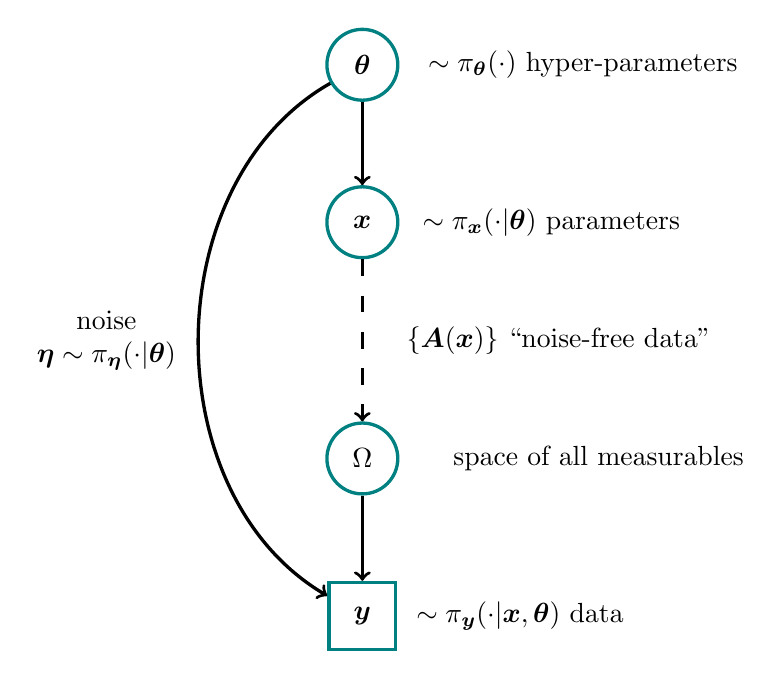
\begin{tikzpicture}
		\node[roundnode2] at (0,3.5) (th)    {$\bm{\theta}$};
		\node[roundnode2] at (0,1.5) (x)    {$\bm{x}$};
		\node[roundnode2] at (0,-1.5) (u)    {$\Omega$};
		\node[rectnode] at (0,-3.5) (y)    {$\bm{y}$};
		
		\draw[->, very thick] (th.south) -- (x.north); 
		\draw[->, very thick, mydotted] (x.south) -- (u.north); 
		\draw[->, very thick] (u.south) -- (y.north); 
		\draw[->, very thick] (th) edge[bend right=60] (y);  
		
		\node[align=center] at (2.8,3.5) (tht) {$\sim \pi_{\bm{\theta}}(\cdot) $ hyper-parameters};
		\node[align=center] at (2.4,1.5) (xt) {$\sim \pi_{\bm{x}}(\cdot|\bm{\theta}) $ parameters};
		\node[align=center] at (2.5,0) (At) {$\{\bm{A}(\bm{x})\}$ ``noise-free data''};
		\node[align=center] at (3,-1.5) (ut) {space of all measurables};
		\node[align=center] at (2,-3.5) (yt) {$\sim \pi_{\bm{y}}(\cdot|\bm{x},\bm{\theta})$ data};
		\node[align=center] at (-3.25,0) (nt) {noise\\$\bm{\eta} \sim \pi_{\bm{\eta}}(\cdot|\bm{\theta})$};
	\end{tikzpicture}
	\caption[Hierarchical Bayesian Model]{A directed acyclic graph (DAG) for an inverse problem visualises statistical dependencies as solid line arrows and deterministic dependencies as dotted arrows.
		The hyper-parameters $\bm{\theta}$ are distributed as ($\sim$) the hyper-prior distribution $\pi(\bm{\theta})$.
		The prior distribution $ \pi_{\bm{x}}(\cdot|\bm{\theta})$ for the parameter $\bm{x}$ and the noise  $\bm{\eta} \sim \pi_{\bm{\eta}}(\cdot|\bm{\theta})$ are statistically dependent on some of those hyper-parameters.
		Then a parameter $\bm{x} \sim \pi_{\bm{x}}(\cdot|\bm{\theta})$ is deterministically mapped onto the space of all measurables $\Omega=\bm{A}(\bm{x})$ through the forward model.
		From the space of all measurable noise-free data we observe (square box) a data set $\bm{y} = \bm{A}(\bm{x}) + \bm{\eta}$ with some additive random noise, which determines the likelihood function $\pi(\bm{y}|\bm{x},\bm{\theta})$.}
	\label{fig:FirstDAG}
\end{figure}

Assume we observe some data
\begin{align}
	\bm{y} = \bm{A} (\bm{x}) + \bm{\eta},
	\label{eq:NonLinDat}
\end{align}
based on a forward model $\bm{A}(\bm{x})$, which may be non-linear, an unknown parameter vector $\bm{x}$ and some additive random noise $\bm{\eta}$.

Naturally, due to the noise, the observation process in Eq. \ref{eq:NonLinDat} is a random process.
Hence, in Bayesian modelling, the aim is to determine a probability distribution over the parameter $\bm{x}$ given some data $\bm{y}$.
Further, a hierarchical Bayesian model incorporates unknown (auxiliary) hyper-parameters $\bm{\theta}$, and treats hyper-parameters and parameters as random variables \cite[Chapter 3]{kaipio2005statinv}.

According to Bayes' theorem, the joint posterior distribution over the parameters $\bm{x}$ and the hyper-parameter $\bm{\theta}$ is given as
\begin{align}
	\pi(\bm{x},\bm{\theta}|\bm{y}) = \frac{ \pi(\bm{y} | \bm{x}, \bm{\theta} ) \pi(\bm{x}, \bm{\theta})}{\pi(\bm{y})} \propto \pi(\bm{y} | \bm{x}, \bm{\theta} ) \pi(\bm{x}, \bm{\theta}) \, ,
\end{align}
with finite and non-zero $\pi(\bm{y})$.
The likelihood function $\pi(\bm{y}|\bm{x},\bm{\theta})$ is defined by the nature of the noise and the noise-free data $\bm{A}(\bm{x})$, which we read as the distribution over $\bm{y}$ conditioned on $\bm{x}$ and $\bm{\theta}$.
Here $\bm{\theta}$ may account for multiple hyper-parameters, e.g. modelling the noise vector $\bm{\eta} \sim \pi_{\bm{\eta}}(\cdot|\bm{\theta})$, where $\sim$ reads as ``is distributed as'', and describing physical properties or functional dependencies of $\bm{x}$ such as the smoothness of $\bm{x}$.
Consequently $\bm{\theta}$ is described by the hyper-prior distribution $\pi(\bm{\theta})$, where $\pi(\bm{x}, \bm{\theta}) = \pi(\bm{x}|\bm{\theta}) \pi(\bm{\theta})$ with the prior distribution $\pi(\bm{x}|\bm{\theta})$.
Choosing these prior distributions is ultimately a modeller's choice and is crucial, as those shall be as uninformative as possible for regions in hyper-parameter and parameter space where the data is informative.
If the data is uninformative, the prior distributions can be informative and represent a rather restrictive range of (physically) feasible hyper-parameters and parameters.

Figure~\ref{fig:FirstDAG} visualises the conditional dependencies between hyper-parameters and parameters as well as how distributions progress through to a observation (square box) using a directed acyclic graph (DAG).
We plot statistical dependencies as solid arrows and deterministic dependencies as dotted arrows.
%\textcolor{red}{conditional dependencies and sqaure box is observation}

% not affect the posterior distribution \textcolor{red}{what, of course the prior affects the posterior. What are you trying to say?}

%$\pi(\bm{x},\bm{\theta}|\bm{y}) $ reads as the distribution of $\bm{x}$ and $\bm{\theta}$ given (conditioned on) the data $\bm{y}$. \textcolor{red}{two sentences, talk anbout posterior and then model }

%Here $\bm{\theta}$ models the random noise $\bm{\eta} \sim \pi_{\bm{\eta}}(\cdot|\bm{\theta})$, 
%The h
%This already incorporates hierarchically ordered modelling as we model the noise thought the hyper-parameters $\bm{\theta}$.
%which we classify through a hyper-parameter, we deal with a random process. \textcolor{red}{Maybe more clear is to say that the observation process (2.1) is a random process.}
%We incorporate that in our hierarchically ordered modelling through the likelihood function $\pi(\bm{y}|\bm{x},\bm{\theta})$, which includes all relevant information captured by the model $\bm{A}(\bm{x})$, and is defined by the measurement process and the nature of the noise. \textcolor{red}{how does the model "capture information"? Oh, do you mean the observation process? Might pay to not use 'model' for lots of things.}
%
%Consequently we define hyper-prior distributions $\pi(\bm{\theta})$ and prior distributions $\pi(\bm{x}|\bm{\theta})$.


%Note that here we include the hyper-parameters within the posterior distribution, which is the key idea of hierarchical Bayesian modelling. \textcolor{red}{"the" key idea? Maybe say that it is intrinsic to Bayes models, or something. You could quote Kaipio and Somersalo that all unknowns are treated as random variables.} \cite[Chapter 3]{kaipio2005statinv}
%


Usually, the objective is to calculate the expectation of a function $h(\bm{x})$, which is defined as
\begin{align}
	\text{E}_{\bm{x},\bm{\theta}|\bm{y}} [h(\bm{x})] =  \underbrace{\int \int   h(\bm{x}) \,  \pi(\bm{x}, \bm{\theta} | \bm{y} ) \, \diff \bm{x}  \, \diff \bm{\theta}}_{\bar{h}}   \label{eq:expPos} \, .
\end{align}
If that is a high-dimensional integral and computationally not feasible to solve, we approximate 
\begin{align}
	\label{eq:sampMean}
	\text{E}_{\bm{x},\bm{\theta}|\bm{y}} [h(\bm{x})] \approx \underbrace{ \frac{1}{N} \sum_{k=1}^{N} h(\bm{x}^{(k)})  }_{\bar{h}_N} \, ,
\end{align}
with an the unbiased sample-based Monte-Carlo estimate \cite{roberts2004general} for large enough $N$ (law of large numbers \cite[Chapter 17]{tweedie2009measprob}).
Here, the posterior samples $\{\bm{x}^{(k)},\bm{\theta}^{(k)} \}\sim \pi_{\bm{x}, \bm{\theta}}(\cdot|\bm{y})$, for $k = 1, \dots, N$, form a sample set $\mathcal{M} =\{ (\bm{x},\bm{\theta})^{(1)}, \dots ,  (\bm{x},\bm{\theta})^{(N)} \}$.
The central limit theorem states that the sample mean $\bar{h}^{(i)}_N $ of independent sample sets $\mathcal{M}^{(i)}\sim\pi (\bm{x}, \bm{\theta}| \bm{y})$, for $i = 1, \dots, n$ from a distribution, converges to be normally distributed, so that
\begin{align}
	\sqrt{n} (\bar{h}^{(i)}_N -  \bar{h} ) \overset{\mathcal{D}}{\longrightarrow} \mathcal{N} (0,\sigma^2) \text{\cite{geyer1992practical}},
\end{align}
and if $\sigma^2 < \infty$ the Monte-Carlo error $\bar{h}^{(i)}_N -  \bar{h} $ is bounded.
In practice, we approximate the Monte-Carlo error from a sample set $\mathcal{M}^{(i)}$ as
\begin{align}
	(\sigma^{(i)})^2  =  \text{Var}(\text{E}_{\bm{x},\bm{\theta}|\bm{y}} [h(\bm{x})]) 
	\approx \frac{\text{Var}(h(\bm{x}) )}{N} \Bigg( \underbrace{  1 + 2 \sum_{t = 1}^{W} \frac{\Gamma(t)}{\Gamma(0)}  }_{ \coloneqq 	\tau_{\text{int}} }\Bigg) = \text{Var}(h(\bm{x})) \frac{ \tau_{\text{int}} }{N} \, , \label{eq:MCerr}
\end{align}
where we have to take into account that the samples generated by any system or algorithm are correlated.
We define the integrated autocorrelation time (IACT) $\tau_{\text{int}}$ as in \cite{fox2016fast}, which is twice the value of the IACT in~\cite[pp. 103-105]{wolff2002LecNot}.
Here the autocorrelation coefficient $\Gamma(t) \propto \exp\{ - |t| /\tau \} \longrightarrow 0$ for $t \rightarrow \infty$ at lag $t$ decays exponentially and $\Gamma(0) =\text{Var}(h(\bm{x}) ) $.
Choosing the summation window $W$ is crucial because it has to be large compared to the decay time $\tau$, but for too large $t$ the autocorrelation coefficient $\Gamma(t)$ is noise-dominated.
U. Wolff \cite{wolff2004monte} (and the Python implementation by D. Hesse \cite{drikHesse}) provide a way to not only calculate the IACT safely but also to quantify the errors of the estimated IACT.

The IACT provides a good estimate of the number of steps the sampling algorithm needs to take to produce one independent sample.
According The IACT, we define the effective sample size as $ \tau_{\text{int}} /N$.
We point out that for uncorrelated samples $\tau_{\text{int}} = 1$ the error $(\sigma^{(i)})^2$ is a typical Monte-Carlo estimate.
See Appendix~\ref{ap:IATC} and~\cite{Sokal1997, wolff2004monte, wolff2002LecNot} for a more detailed derivation.

\subsection{Marginal and then Conditional Method}
\label{subsec:TheoMTC}
Quickly generating a representative sample set from the posterior distribution often presents a significant challenge. This is mainly \textcolor{red}{this word is misplaced (for English). Better is Quickly generating (it's an adverb)} due to the strong correlations that usually exist between the parameters and hyper-parameters, as discussed by Rue and Held in~\cite{rue2005gaussian} and illustrated in Appendix~\ref{ap:Correlation}.
If $\bm{x}$ cannot be parametrised directly in terms of the hyper-parameters $\bm{\theta}$, so that $\bm{x}(\bm{\theta})$ is function of $\bm{\theta}$, it is beneficial to factorise the posterior distribution as \textcolor{red}{this is unclear. Of course x(theta) is a function of theta. What are you trying to say?}
\begin{align}
	\pi(\bm{x}, \bm{\theta} |  \bm{y}) = \pi(\bm{x} |  \bm{\theta}, \bm{y}) \, \pi(\bm{\theta} |   \bm{y}), \label{eq:MTC}
\end{align}
into the full conditional posterior $\pi(\bm{x} |  \bm{\theta}, \bm{y})$ over the latent field $\bm{x}$ and the marginal posterior over the hyper-parameter $\bm{\theta}$, that can be calculated by,
\begin{align}
	\pi(\bm{\theta} |   \bm{y}) =  \frac{ \pi(   \bm{y} | \bm{x},\bm{\theta})  \pi( \bm{x} | \bm{\theta} )  \pi(\bm{\theta}) }{ \pi(\bm{x} | \bm{\theta} ,   \bm{y})   \pi( \bm{y})} \propto \frac{ \pi(   \bm{y} | \bm{x},\bm{\theta})  \pi( \bm{x} | \bm{\theta} )  \pi(\bm{\theta}) }{ \pi(\bm{x} | \bm{\theta} ,   \bm{y}) } \label{eq:margGen}\, ,
\end{align}
as in~\cite[Lemma 2]{fox2016fast}.
%In \cite{norton2018sampling}, they classify inverse problems into problems with known or unknown conditional posterior distributions, and conclude that if $\pi(\bm{x} | \bm{\theta} ,   \bm{y}) = \pi(\bm{y} | \bm{x}, \bm{\theta} ) \pi(\bm{x}| \bm{\theta})  / \pi(   \bm{y}| \bm{\theta})$ has a known form, the normalising constant of $\pi(\bm{\theta} |   \bm{y})$ is available \newline $\int \pi(\bm{y} | \bm{x}, \bm{\theta} ) \pi(\bm{x}| \bm{\theta}) \text{d} \bm{x} = \pi(   \bm{y}| \bm{\theta})  \propto \pi( \bm{\theta}|\bm{y}) / \pi(\bm{\theta})$ and one can almost surely determine the $\bm{\theta}$-dependence of the marginal posterior $\pi(\bm{\theta} |   \bm{y})$.

This approach, known as the MTC method, is particularly advantageous when $\bm{x}\in \mathbb{R}^n$ is high-dimensional, while $\bm{\theta}\in \mathbb{R}^{n_{\bm{\theta}}}$ is low-dimensional, so that $n_{\bm{\theta}} \ll n$ and the evaluation of $\pi(\bm{\theta}| \bm{y})$ is relatively cheap. \textcolor{red}{horrible notation, try better.}
Applying the law of total expectation~\cite{champ2022generalizedlawtotalcovariance}, Eq.~\eqref{eq:expPos} becomes
\begin{align}
	\mathbb{E}_{\bm{x} ,\bm{\theta}  |\bm{y}} [h(\bm{x})] &= \int \int   h(\bm{x}) \pi(\bm{x} |  \bm{\theta}, \bm{y}) \, \diff \bm{x} \,  \pi(\bm{\theta} |   \bm{y}) \, \diff \bm{\theta} \\
	&= \int \mathbb{E}_{\bm{x} |  \bm{\theta}, \bm{y}} \left[ h(\bm{x}) \right] \, \pi(\bm{\theta} |  \bm{y}) \, \diff \bm{\theta}\label{eq:2fullCond} \\
		&= \mathbb{E}_{\bm{\theta} |  \bm{y}} \left[ \mathbb{E}_{\bm{x} |  \bm{\theta}, \bm{y}} [h(\bm{x})] \right] \, .
	\label{eq:fullCond}
\end{align}
In the case of a linear-Gaussian hierarchical Bayesian model, both the marginal distribution $\pi (\bm{\theta}| \bm{y})$ %\textcolor{red}{separate sentence (You have a tendency to let sentences wander to different ideas. Split into single topics.)} 
and the inner expectation $\mathbb{E}_{\bm{x} |  \bm{\theta}, \bm{y}} \left[ h(\bm{x}) \right]$ are well defined (see next subsection).
If the integral in Eq.~\ref{eq:2fullCond} is expensive to calculate, we use sample-based methods to produce a Markov chain $\{ (\bm{x}, \bm{\theta})^{(1)}, \dots, (\bm{x}, \bm{\theta})^{(N)} \} \sim \pi(\bm{x}, \bm{\theta} |  \bm{y}) $ and sample from $\pi(\bm{\theta} |  \bm{y})$ first and then draw samples from the full conditional posterior $\pi(\bm{x} | \bm{\theta} , \bm{y})$, e.g via the RTO method (see Sec.~\ref{subsec:RTO}). 


\subsubsection{Linear-Gaussian hierarchical Bayesian model}
\label{subsec:LinBay}
In case of normally distributed noise $\bm{\eta} \sim \mathcal{N}(\bm{0},\bm{\Sigma}(\bm{\theta}))$ with zero mean and covariance $\bm{\Sigma}(\bm{\theta})$ and a linear forward model matrix $\bm{A}$ the Eq.~\ref{eq:NonLinDat} simplifies to
\begin{align}
	\bm{y} = \bm{A} \bm{x} + \bm{\eta} \, .
	\label{eq:LinDat}
\end{align}
Then we can obtain the marginal and full conditional posterior distribution explicitly.
Our hierarchical linear-Gaussian Bayesian model is defined as
\begin{subequations}
	\label{eq:GenBayMode}
	\begin{align}
		\bm{y} |  \bm{x}, \bm{\theta} &\sim \mathcal{N}(\bm{A} \bm{x}, \bm{\Sigma}(\bm{\theta}) ) \\
		\bm{x} |  \bm{\theta} &\sim \mathcal{N}(\bm{\mu}, \bm{Q}(\bm{\theta})^{-1} ) \\
		\bm{\theta} &\sim \pi(\bm{\theta}) \,  ,
	\end{align}
\end{subequations}
with a Gaussian likelihood function $\pi(\bm{y} | \bm{x}, \bm{\theta} )$, a normally distributed prior $\pi(\bm{x}|\bm{\theta})$, with prior mean $\bm{\mu}$ and prior precision $\bm{Q}(\bm{\theta})$, and a hyper-prior distribution $\pi(\bm{\theta})$.
For derivation of the marginal posterior and the full conditional posterior distribution, consider the joint multivariate Gaussian distribution
\begin{align}
	\begin{pmatrix}
		\bm{x} \\
		\bm{y}
	\end{pmatrix}\sim \mathcal{N}\left[  \begin{pmatrix}
		\bm{\mu} \\
		\bm{A}\bm{\mu}
	\end{pmatrix},\begin{pmatrix}
		\bm{Q}(\bm{\theta}) + \bm{A}^T \bm{\Sigma}(\bm{\theta})^{-1} \bm{A} & - \bm{A}^T \bm{\Sigma}(\bm{\theta})^{-1} \\
		\bm{\Sigma}(\bm{\theta})^{-1} \bm{A} & \bm{\Sigma}(\bm{\theta})^{-1} 
	\end{pmatrix}^{-1} \right] \, , 	\label{eq:jointMultiGaus}
\end{align}
with the joint precision matrix as in~\cite{SIMPSON201216} (see also~\cite{rue2005gaussian, fox2016fast}).
Immediately, the full conditional posterior distribution can be formulated as 
\begin{align}
	\bm{x} | \bm{\theta} , \bm{y}\sim \mathcal{N}\big(\underbrace{ \bm{\mu} + (\bm{Q}(\bm{\theta}) + \bm{A}^T \bm{\Sigma}(\bm{\theta})^{-1} \bm{A})^{-1}(\bm{y} - \bm{A}\bm{\mu})}_{\bm{\mu}_{\bm{x} | \bm{\theta} , \bm{y}}},\underbrace{ (\bm{Q}(\bm{\theta}) + \bm{A}^T \bm{\Sigma}(\bm{\theta})^{-1} \bm{A})^{-1}}_{\bm{\Sigma}_{\bm{x} | \bm{\theta} , \bm{y}}} \big)\, \label{eq:CondPostLin}.
\end{align}
Then the marginal posterior distribution over the hyper-parameters is derived as in Eq. \ref{eq:margGen}, where, as noted by Fox and Norton~\cite{fox2016fast}, the parameter $\bm{x}$ cancels and we arrive at
\begin{align}\begin{split}
		\pi(\bm{\theta} | \bm{y}) \propto & \sqrt{\frac{\det{(\bm{\Sigma}(\bm{\theta})^{-1})} \det{(\bm{Q}(\bm{\theta}))} }{\det{(\bm{Q}(\bm{\theta}) + \bm{A}^T \bm{\Sigma}(\bm{\theta})^{-1} \bm{A})} } }  \exp \Bigg\{  -\frac{1}{2} (\bm{y} - \bm{A} \bm{\mu})^T \\ &\big[ \bm{\Sigma}(\bm{\theta})^{-1} - \bm{\Sigma}(\bm{\theta})^{-1} \bm{A}  (\bm{Q}(\bm{\theta}) + \bm{A}^T \bm{\Sigma}(\bm{\theta})^{-1} \bm{A})^{-1} \bm{A}^T \bm{\Sigma} (\bm{\theta})^{-1} \big] (\bm{y} - \bm{A} \bm{\mu}) \Bigg\} \pi(\bm{\theta}) \, .
	\end{split} 
\end{align} 
Having the marginal posterior distribution $\pi (\bm{\theta}| \bm{y})$ (independent of $\bm{x}$) available breaks up the correlation structure between $\bm{x}$ and $\bm{\theta}$ and makes the MTC approach very efficient~\cite{fox2016fast} (see Appendix~\ref{ap:Correlation}).
Within this scheme, we evaluate the marginal posterior first and then either condition on hyper-parameters to draw full conditional posterior samples $\bm{x} \sim \pi (\bm{x} | \bm{\theta}, \bm{y})$ (see Sec.~\ref{subsec:RTO}) or evaluate the mean
\begin{align}
	\mu_{\bm{x}|\bm{y}} = \int \bm{\mu}_{\bm{x} | \bm{\theta} , \bm{y}} \pi(\bm{\theta}| \bm{y}) \diff \bm{\theta} \label{eq:MeanGenInt}
\end{align} and covariance matrix
\begin{align}
	\Sigma_{\bm{x}|\bm{y}} = \int \bm{\Sigma}_{\bm{x} | \bm{\theta} , \bm{y}} \pi(\bm{\theta}| \bm{y}) \diff \bm{\theta}\label{eq:CoVarGenInt}
\end{align}
of the posterior $\pi(\bm{x}| \bm{y})$ by some quadrature rule.

\section{Ergodicity of MCMC chains}
Because we are using the mTC method we draw sampples from the marginal posterio ifrat using MCMC methods ant hen from  to gernatea marhkov chain from the marginal distributon


Ergditcy is imoprtatn to show that we dar sample from the dsitribution
In this section we present the methods that draw samples from the marginal posterior $ \mathcal{M} = \{  \bm{\theta}^{(1)}, \dots,  \bm{\theta}^{(k)}, \dots, \bm{\theta}^{(N)} \} \sim \pi(\bm{\theta} |  \bm{y})$ \textcolor{red}{this reads as if M is the marginal posterior. Rewrite.} as well as the RTO method to draw samples from a normally distributed full conditional posterior $\pi(\bm{x}|\bm{\theta} , \bm{y})$. \textcolor{red}{what is the "full posterior" as opposed to the "posterior"?}
Here, $\mathcal{M}$ denotes a Markov chain, where each new sample $\bm{\theta}^{(k)}$ is only affected by the previous one $\bm{\theta}^{(k-1)}$.
MCMC methods generate such a chain $\mathcal{M}$ using random (Monte-Carlo) proposals $(\bm{x}, \bm{\theta})^{(k)} \sim q( \cdot |  \bm{\theta}^{(k-1)})$ \textcolor{red}{This is defining "Markov". . Be more explicit.} according to a proposal distribution conditioned on the previous sample (Markov), where ergodicity of the chain $\mathcal{M}$ is a sufficient criterion for using sample-based estimates~\cite{tan2016LecNot, roberts2004general}. \textcolor{red}{you are a little unclear about a chain of random variables, and an instance of such a chain.}

The ergodicity theorem in~\cite{tan2016LecNot} states that, if a Markov chain $\mathcal{M}$ is aperiodic, irreducible, and reversible, then it converges to a unique stationary equilibrium distribution.
In other words, the chain can reach any state from any other state (irreducibility), is not stuck in periodic cycles (aperiodicity), and satisfies the detailed balance condition~\cite{tan2016LecNot} (reversibility).
Then the samples in that chain $ \mathcal{M} \sim \pi( \bm{\theta} |  \bm{y})$ are samples from the desired target distribution.
In practice, one can inspect the trace $\pi(\bm{\theta}^{(k)} |  \bm{y})$ for $k = 1, \dots, N$ and visually assess convergence  \textcolor{red}{converge to, so after 'burn in'}  period.
and mixing properties of the chain to evaluate if the behavours is consistent with ergodicty.
\textcolor{red}{this is a bit loose. really, one evaluates if the behaviour is consistent with ergodicity.}
The sampling methods used in this thesis possess proven ergodic properties, and we therefore refer the reader to the corresponding literature for further details. 

If the Markov chain over the marginal posterior $\pi(\bm{\theta} |  \bm{y})$ is ergodic \textcolor{red}{reference Jun Liu, or something.}, and the full conditional samples $\bm{x}^{(k)} \sim \pi(\bm{x}|   \bm{\theta}^{(k)}, \bm{y})$ are drawn independently, as e.g. in Sec.~\ref{subsec:RTO}, then the resulting joint chain $\{ (\bm{x}, \bm{\theta})^{(1)}, \dots, (\bm{x}, \bm{\theta})^{(N)} \} \sim \pi(\bm{x}, \bm{\theta} |  \bm{y}) =  \pi(\bm{x} |  \bm{\theta} , \bm{y}) \pi( \bm{\theta} | \bm{y})$ is also ergodic \textcolor{red}{for the posterior}~\cite{acosta2022markov}. \textcolor{red}{strictly, ergodic for [theta|y] -- ergodicity is with respect to a particular distribution.}


\section{Numerical Approximation -- Tensor-Train (TT)}
\label{sec:tensortrain}
%\textcolor{red}{Explain how to find normalisation constant and say that due to aproxiamting the sqaure root we ensure posivyt later when squaring it}
%First, we provide a short overview of probability spaces and their associated measures. 
%I am not claiming this overview to be complete but consider it helpful to understand the notation in \cite{cui2022deep}, which we follow to approximate functions in the TT format.
Instead of relying on sampling-based methods to explore a target distribution $\pi(\bm{x})$, we can approximate this distribution on a $d$-dimensional grid using a tensor-train (TT) approximation $\tilde{\pi}(\bm{x}) \approx \pi(\bm{x})$, where $\bm{x} \in \mathbb{R}^d$, with far fewer function evaluation compared to conventional sampling methods.
In the following, we describe how to compute marginal distributions from a probability density approximated in TT \textcolor{red}{ (tensor train)} format and how to generate samples using the inverse Rosenblatt transform (IRT) as in \cite{dolgov2020approximation}, following the notation and procedure introduced in~\cite{cui2022deep}.
\textcolor{red}{We represent a probability distribution on a d-dimensional grid with grid points n in each dimension.
I'm surprised that you never cite the Approximation an Sampling paper that introduced the idea of TT approximation of PDFs. Oh, you do, but the author list is abbreviated. Don't abbreviate the author list fro a thesis.}
As in~\cite{cui2022deep}, we can define the parameter space as the product space $\mathcal{X} = \mathcal{X}_1 \times \mathcal{X}_2 \times \dots \times \mathcal{X}_d$ with $ x_k \in \mathcal{X}_k \subseteq \mathbb{R}$.
% and $\bm{x} = ( x_1,\dots ,x_k,\dots,x_d )$.
The marginal density function for the $k$-th component is then given by
\begin{align}
	f_{X_k}(x_k) = \frac{1}{z} \int_{\mathcal{X}_1} \cdots \int_{\mathcal{X}_{k-1}} \int_{\mathcal{X}_{k+1}} \cdots  \int_{\mathcal{X}_d} \uplambda(\bm{x}) \, \pi(\bm{x}) \, \diff x_1 \cdots \diff x_{k-1} \, \diff x_{k+1} \cdots \diff x_d, \label{eq:margInt}
\end{align}
where we integrate over all dimensions except the $k$-th, and $z$ is a normalisation constant.
Here, Cui and Dolgov~\cite{cui2022deep} refer to $\uplambda(x)$ as the ``product-form Lebesgue-measurable weighting function'', which can be useful for quadrature rules~\cite{davis2007methods}, and define it as
\begin{align}
	\uplambda(\mathcal{X}) = \prod_{i = 1}^{d} \uplambda_i(\mathcal{X}_i), \quad \text{where} \quad \uplambda_i(\mathcal{X}_i) = \int_{\mathcal{X}_i} \uplambda_i(x_i) \, \diff x_i. \label{eq:lebesgueWeight}
\end{align}

In the TT format, the integral in Eq.~\ref{eq:margInt} for the marginal probability can be computed at a low computational cost, as $\pi(\bm{x})$ is approximated by
\begin{align*}
	\tilde{\pi}(\bm{x}) = 	\tilde{\pi}_1(x_1)  \tilde{\pi}_2(x_2)  \cdots \tilde{\pi}_d(x_d),
\end{align*}
which is a sequence of matrix multiplications with $\tilde{\pi}_k(x_k) \in \mathbb{R}^{r_{k-1} \times r_k}$ for a fixed point $\bm{x} = (x_1, \dots, x_d)$ on a predefined $d$-dimensional discrete univariate grid over the parameter space $\mathcal{X}$. 
A TT core  $\tilde{\pi}_k \in \mathbb{R}^{r_{k-1} \times n \times r_k}$ has ranks $ r_{k-1}$ and $r_k$, which are connecting the TT core to its respective neighbouring dimensions.
A TT train has outer ranks $r_0 = r_d = 1$.  \textcolor{red}{more sentence creep. You should have defined the univariate grids, earlier.}
This enables us to approximate $\pi(\mathcal{X})\approx \tilde{\pi}_1  \tilde{\pi}_2  \cdots \tilde{\pi}_d$ over a discrete parameter space $\mathcal{X}$ using $2nr + (d-2)nr^2$ evaluation points for fixed ranks $r =r_{k-1} = r_k $, as illustrated in Figure~\ref{fig:TTfig}, instead of $n^d$ function evaluation.
Consequently, the marginal target distribution
\begin{align}
	\begin{split}
		f_{X_k}(x_k) \approx \frac{1}{z} \Big|\, 
		&\left( \int_{\mathcal{X}_1} \uplambda_1(x_1) \tilde{\pi}_1(x_1) \, \diff x_1 \right) \cdots 
		\left( \int_{\mathcal{X}_{k-1}} \uplambda_{k-1}(x_{k-1}) \tilde{\pi}_{k-1}(x_{k-1}) \, \diff x_{k-1} \right) \\
		&\quad \uplambda_k(x_k) \tilde{\pi}_k(x_k) \\
		& \left( \int_{\mathcal{X}_{k+1}} \uplambda_{k+1}(x_{k+1}) \tilde{\pi}_{k+1}(x_{k+1}) \,\diff x_{k+1} \right) \cdots 
		\left( \int_{\mathcal{X}_{d}} \uplambda_d(x_d) \tilde{\pi}_d(x_d) \, \diff x_d \right)
		\Big| 
	\end{split}
\end{align}
is computed by integrating over all TT cores except the $k$-th core $\pi_k$, as in~\cite{dolgov2020approximation}, and normalised by the constant $z$~\cite{cui2022deep}.

\begin{figure}[ht!]
	\centering
\begin{subfigure}{\textwidth}
	\input{TTSchem.pdf_tex}
	\caption{}
\end{subfigure}
	\centering
\begin{subfigure}{\textwidth}
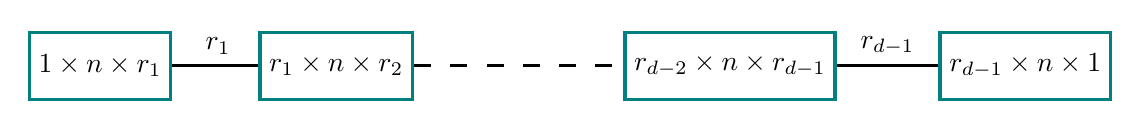
\begin{tikzpicture} 
	\node[rectnode] at (-5,0) (T1)    {$1 \times n \times r_1$};
	\node[rectnode] at (-2,0) (T2)    {$r_1 \times n \times r_{2}$};
	
	\node[rectnode] at (3,0) (Tn1)    {$r_{d-2} \times n \times r_{d-1} $};
	\node[rectnode] at (6.75,0) (Tn)    {$r_{d-1} \times n \times 1$};
	\draw[-, very thick] (T1.east) -- (T2.west); 
	\draw[-, very thick] (Tn.west) -- (Tn1.east); 
	\draw[-, mydotted, very thick] (T2.east) -- (Tn1.west);
	
	\node[align=center] at (-3.5,0.25) (R) {$r_1$};
	\node[align=center] at (5,0.25) (R) {$r_{d-1}$};	
\end{tikzpicture} 
	\caption{}
\end{subfigure}
\caption[Visualisation of a tensor train]{Here, we visualise the TT cores as a train of two- and three-dimensional matrices. 
Each core has a length $n$, corresponding to the number of grid points in each dimension, and the cores are connected through ranks $r_k$. 
More specifically, a core $\tilde{\pi}_k$ has dimensions $r_{k-1} \times n \times r_k$, with outer ranks $r_0 = r_d = 1$.
Using the TT format enables us to represent a $d$-dimensional grid with only $2nr + (d-2)nr^2$ evaluation points instead of $n^d$ grid points.
Figure~(a) is adapted from~\cite{fox2021grid}.}
\label{fig:TTfig}
\end{figure}


%%%%%% Squared and Basis Function %%%%%
In practice, TT approximations may suffer from numerical instability, in particular because it is not advantageous yet to approximate the target function $\pi(\bm{x})$ in e.g. the logarithmic space. 
Hence, Cui et al.~\cite{cui2022deep} approximate the square root of the probability density \textcolor{red}{Thsi sentence needs rewriting - -it's a jumble of ideas.
	Hence implies an implication -- is it that or just one possible resolution?}
\begin{align}
	\sqrt{\pi(\bm{x})} \approx \tilde{g}(\bm{x}) = \bm{G}_1(x_1), \dots, \bm{G}_k(x_k), \dots, \bm{G}_d(x_d)\, \,  \text{\cite[Eq. 18]{cui2022deep}},
\end{align}
which ensures positivity.
%and intuitively ``reduces the range of numbers'' (excuse this unmathematical expression).
Here, each TT core is given by
\begin{equation}
	G^{(\alpha_{k-1},\alpha_k)}_k(x_k) = \sum_{i=1}^{n_k} \phi^{(i)}_k(x_k) \bm{A}_k[\alpha_{k-1}, i, \alpha_k], \quad k = 1, \dots, d,\, \,  \text{\cite[Eq. 21]{cui2022deep}},
\end{equation}
where $\bm{A}_k \in \mathbb{R}^{r_{k-1} \times n_k \times r_k}$ is the $k$-th coefficient tensor and $\{\phi^{(i)}_k(x_k)\}_{i=1}^{n_k}$ are the basis functions corresponding to the $k$-th coordinate.
The approximated unnormalised density is written as: \textcolor{red}{put the reference in the text. Immediately prior is probably best.}
\begin{align}
	\pi(\bm{x}) \approx \xi + \tilde{g}(\bm{x})^2\, \,  \text{\cite[Eq. 19]{cui2022deep}},
\end{align}
where $\xi$ is a positive constant added according to the ratio of the Lebesgue weighted L2-norm error and the Lebesgue weighting (see Eq.~\ref{eq:lebesgueWeight}) such that
\begin{align}
	0 \leq \xi \leq \frac{1}{\uplambda(\mathcal{X})} \lVert \tilde{g} - \sqrt{\pi} \rVert_{L^2_{\uplambda}(\mathcal{X})}^2\, \,  \text{\cite[Eq. 35]{cui2022deep}}. \label{eq:gamErr}
\end{align}
This leads to the normalised target function
\begin{align}
	f_X(\bm{x})  \approx \frac{1}{z} \left( \uplambda(\bm{x}) \xi  + \uplambda(\bm{x}) \tilde{g}(\bm{x})^2 \right)\, \,  \text{\cite[Eq. 19]{cui2022deep}},
\end{align}
with the normalisation constant $z = \int_{\mathcal{X}} f_X(\bm{x}) \diff \bm{x} $.
Given the tensor train approximation of $\sqrt{\pi}$, the marginal function $f_{X_k}(x_k)$ can be expressed as
\begin{align}
	\begin{split}
		f_{X_k}(x_k)  \approx \frac{1}{z} \Bigg(&\xi \prod_{i=1}^{k-1} \uplambda_i(\mathcal{X}_i) \prod_{i=k+1}^{d} \uplambda_i(\mathcal{X}_i) \\
		&+ \left( \int_{\mathcal{X}_1} \uplambda_1(x_1) \bm{G}_1^2(x_1)  \, \diff x_1 \right) \cdots 
		\left( \int_{\mathcal{X}_{k-1}} \uplambda_{k-1}(x_{k-1}) \bm{G}_{k-1}^2(x_{k-1}) \, \diff x_{k-1} \right) \\
		& \uplambda_k(x_k) \bm{G}_k^2(x_k)  \\
		&\left( \int_{\mathcal{X}_{k+1}} \uplambda_{k+1}(x_{k+1}) \bm{G}_{k+1}^2(x_{k+1})  \,\diff x_{k+1} \right) \cdots 
		\left( \int_{\mathcal{X}_d} \uplambda_d(x_d) \bm{G}_d^2(x_d)  \, \diff x_d \right) \Bigg).
	\end{split}
\end{align}




\subsection{Marginal Probability Distributions}
\label{subsec:TTMarg}
We compute the marginal probability distributions by a procedure to which Cui et al.~\cite{cui2022deep} refer to as backwards marginalisation, see Prop.~\ref{prob:ForMarg}, and to which we add the forward marginalisation, see Prop.~\ref{prob:backMarg}. \textcolor{red}{By now you have refered to multiple marginal distributions, so you'll need to be more clear.}
This is similar to the left and right orthogonalisation of TT \textcolor{red}{why abbreviate?} cores~\cite{oseledets2011tensor, Oseledets2011DMRG}.
The backwards marginalisation provides us with the coefficient matrices $\bm{B}_k$, while the forward marginalisation gives the coefficient matrices $\bm{R}_{\text{pre}, k}$. 
These matrices enable the efficient evaluation of marginal functions since they integrate over the coordinates either left or right of the $k$-th dimension, as in~\cite{cui2022deep}. \textcolor{red}{are they marginal functions or marginal distributions. Pick a language and stick to it.}
In doing so, the mass matrix $\bm{M}_k \in \mathbb{R}^{n_k \times n_k}$ is defined as
\begin{equation}
	\bm{M}_k[i, j] = \int_{\mathcal{X}_k} \phi^{(i)}_k(x_k) \phi^{(j)}_k(x_k) \uplambda(x_k) \, \diff x_k, \quad i, j = 1, \dots, n_k, \, \,  \text{\cite[Eq. 22]{cui2022deep}} \label{eq:MassMat},
\end{equation}
where $\{\phi^{(i)}_k(x_k)\}_{i=1}^{n_k}$ denotes the set of basis functions for the $k$-th coordinate.
The proposition used to compute $\bm{B}_k$, stated in Prop.~\ref{prob:backMarg}, is adapted directly from~\cite{cui2022deep}.

After computing the coefficient tensors $\bm{R}_{\text{pre},k-1}$ as in Prop.~\ref{prob:ForMarg} and $\bm{B}_{k}$ from Prop.~\ref{prob:backMarg}, the marginal PDF of $k$-th dimension can be expressed as
\begin{equation}
	f_{X_k}(x_k)  \approx \frac{1}{z} \left(\xi \prod_{i=1}^{k-1} \uplambda_i(X_i) \prod_{i=k+1}^{d} \uplambda_i(X_i) + \sum_{l_{k-1}=1}^{r_{k-1}} \sum_{l_k=1}^{r_k} \left(\sum_{i=1}^{n} \phi^{(i)}_k(x_k) \bm{D}_k[l_{k-1},i, l_k] \right)^2 \right) \uplambda_k(x_k), \label{eq:MargTT}
\end{equation}
where $\bm{D}_k \in \mathbb{R}^{r_{k-1} \times n \times r_k}$ and given as
\begin{equation}
	\bm{D}_k[l_{k-1},i,l_k] = \sum_{\alpha_{k-1}=1}^{r_{k-1}}  \bm{R}_{\text{pre},k-1}[l_{k-1}, \alpha_{k-1}] \bm{B}_k[\alpha_{k-1}, i, l_k] \, ,
\end{equation}
with $\bm{R}_{\text{pre},k-1}\in \mathbb{R}^{r_{k-1} \times r_{k-1}}$ and $\bm{B}_k \in \mathbb{R}^{r_{k-1} \times n \times r_k}$.

For the first dimension, $f_{X_1}(x_1)$ can be expressed as
\begin{equation}
	f_{X_1}(x_1)  \approx \frac{1}{z} \left(\xi \prod_{i=2}^{d} \uplambda_i(\mathcal{X}_i) + \sum_{l_1=1}^{r_1} \left(\sum_{i=1}^{n} \phi^{(i)}_1(x_1) \bm{D}_1[i, l_1] \right)^2 \right) \uplambda_1(x_1)\, \,  \text{\cite[Eq. 30]{cui2022deep}},
	\label{eq:firstMarg}
\end{equation}
where $\bm{D}_1[i, l_1] = \bm{B}_1[\alpha_0, i, l_1]$ and $\alpha_0 = 1$,
and similarly in the last dimension
\begin{equation}
	f_{X_d}(x_d)  \approx \frac{1}{z} \left(\xi \prod_{i=1}^{d-1} \uplambda_i(\mathcal{X}_i) + \sum_{l_{d-1}=1}^{r_{d-1}} \left(\sum_{i=1}^{n} \phi^{(i)}_1(x_1) \bm{D}_d[l_{d-1},i] \right)^2 \right) \uplambda_d(x_d),
\end{equation}
where $\bm{D}_d[l_{d-1},i] = \bm{B}_{\text{pre},d}[l_{d-1}, i, \alpha_{d+1}]$ and $\alpha_{d+1} = 1$.
Note that in practice we calculate $z$ numerically within the process of computing the marginals so that  $\sum f_{X_k}(x_k) =1 $ and for Cartesian basis $\bm{M}_k = \text{diag}(\uplambda_k(\mathcal{X}_k))$ where we set $\uplambda(x) = 1$.

\begin{prop}[Backwards Marginalisation as in~\cite{cui2022deep}]
	\label{prob:backMarg}
	Starting with the last coordinate $k = d$, we set $\bm{B}_d = \bm{A}_d$. The following procedure can be used to obtain the coefficient tensor $\bm{B}_{k} \in \mathbb{R}^{r_{k-1} \times n_{k} \times r_{k}}$, which we need for defining the marginal function $f_{X_k}(x_k)$ or to draw samples from $\tilde{\pi}(\bm{x})$ via the squared IRT scheme (see Alg. Box~\ref{alg:SIRT}):
	\begin{enumerate}
		\item Use the Cholesky decomposition of the mass matrix, $\bm{L}_k \bm{L}_k^\top = \bm{M}_k \in \mathbb{R}^{n_k \times n_k}$, to construct a tensor $\bm{C}_k \in \mathbb{R}^{r_{k-1} \times n_k \times r_k}$:
		\begin{equation}
			\bm{C}_k[\alpha_{k-1}, \tau, l_k] = \sum_{i=1}^{n_k} \bm{B}_k[\alpha_{k-1}, i, l_k] \bm{L}_k[i, \tau] \text{\cite[Eq. (27)]{cui2022deep}}. \label{eq:constrCBack}
		\end{equation}
		\item Unfold $\bm{C}_k$ along the first coordinate and compute the thin QR decomposition, so that $\bm{C}_k^{(R)} \in \mathbb{R}^{r_{k-1} \times (n_k r_k)}$:
		\begin{equation}
			\bm{Q}_k \bm{R}_k = {(\bm{C}_k^{(R)})}^{\top} \, \,  \text{\cite[Eq. 28]{cui2022deep}}.\label{eq:thinQRBack}
		\end{equation}
		\item Compute the new coefficient tensor:
		\begin{equation}
			\bm{B}_{k-1}[\alpha_{k-2}, i, l_{k-1}] = \sum_{\alpha_{k-1}=1}^{r_{k-1}} \bm{A}_{k-1}[\alpha_{k-2}, i, \alpha_{k-1}] \bm{R}_k[l_{k-1}, \alpha_{k-1}]\, \,  \text{\cite[Eq. 29]{cui2022deep}}. \label{eq:nextCoeffTBack}
		\end{equation}
	\end{enumerate}
\end{prop}

\begin{prop}[Forward Marginalisation]
	\label{prob:ForMarg}
	Starting with the first coordinate $k = 1$, we set $\bm{B}_{\text{pre},1} = \bm{A}_1$. The following procedure can be used to obtain $\bm{R}_{\text{pre},k-1} \in \mathbb{R}^{r_{k-1}  \times r_{k-1}}$ for defining the marginal function $f_{X_k}(x_k)$:
	\begin{enumerate}
		\item Use the Cholesky decomposition of the mass matrix, $\bm{L}_k \bm{L}_k^\top = \bm{M}_k \in \mathbb{R}^{n_k \times n_k}$, to construct a tensor $\bm{C}_k \in \mathbb{R}^{r_{k-1} \times n_k \times r_k}$:
		\begin{equation}
			\bm{C}_{\text{pre},k}[\alpha_{k-1}, \tau, l_k] = \sum_{i=1}^{n_k} \bm{L}_k[i, \tau] \bm{B}_{\text{pre},k}[\alpha_{k-1}, i, l_k] .\label{eq:constrCForw}
		\end{equation}
		\item Unfold $\bm{C}_{\text{pre},k}$ along the first coordinate and compute the thin QR decomposition, so that $\bm{C}_{\text{pre},k}^{(R)} \in \mathbb{R}^{(r_{k-1} n_k ) \times r_k}$:
		\begin{equation}
			\bm{Q}_{pre,k}\bm{R}_{\text{pre},k} = {(\bm{C}_{\text{pre},k}^{(R)})}.\label{eq:thinQRForw}
		\end{equation}
		\item Compute the new coefficient tensor $\bm{B}_{\text{pre}, k+1} \in \mathbb{R}^{r_{k-1} \times n_k \times r_k} $:
		\begin{equation}
			\bm{B}_{\text{pre}, k+1}[l_{k+1}, i, \alpha_{k+1}] = \sum_{\alpha_{k}=1}^{r_{k}} \bm{R}_{\text{pre},k}[l_{k+1}, \alpha_{k}] \bm{A}_{k+1}[\alpha_{k}, i, \alpha_{k+1}] .\label{eq:nextCoeffTForw}
		\end{equation}
	\end{enumerate}
\end{prop}


\subsection{Sampling from a TT Approximation}
\label{subsec:SamplTT}
Instead of evaluating marginal functions for quadrature, we can draw samples from the approximated function in the TT format via the inverse Rosenblatt transform, as in \cite{dolgov2020approximation}.
Since the square root of the target function is approximated, Cui and Dolgov~\cite{cui2022deep} call that the squared inverse Rosenblatt transform (SIRT).

\begin{algorithm}[!th]
	\caption{Squared Inverse Rosenblatt Transform (SIRT)}
	\begin{algorithmic}[1]
		\STATE \textbf{Input:} seeds $\{ \bm{u}^{(1)},\dots, \bm{u}^{(N)} \} \sim \mathcal{U}(0,1)^d $ and $\bm{B}_1 , \dots,\bm{B}_d$  from Prop.~\ref{prob:backMarg}
		\FOR{ \( s = 1, \dots, N\)}
		\FOR{ \( k = 1, \dots, d\)}
		\STATE compute normalised PDF $ f_{X_k|X_{<k}}(x_k|x^{(s)}_{k-1},\dots,x^{(s)}_1)$, Eq.~\ref{eq:CurrMarg}
		\STATE compute cumulative distribution function $F_{X_k|X_{<k}}(x_k)$, Eq.~\ref{eq:CurrCDF},
		\STATE project sample $x^{(s)}_k = F_{X_k|X_{<k}}^{-1}(u^{(s)}_k)$
		\STATE interpolate $\bm{G}_k(x^{(s)}_k)$, Eq. \ref{eq:LinPol}
		\STATE update $\bm{G}_{\leq k}(x^{(s)}_{\leq k}) = \bm{G}_{<k}(x^{(s)}_{<k}) \bm{G}_k(x^{(s)}_k)$
		\ENDFOR
		\ENDFOR
		\STATE \textbf{Output:} samples $\{ \bm{x}^{(1)},\dots, \bm{x}^{(N)} \} $, where each $\bm{x}^{(s)} \in \mathbb{R}^d$ for $s = 1, \dots, N$
	\end{algorithmic}
	\label{alg:SIRT}
\end{algorithm}
Given the Backward marginals $\bm{B}_1 , \dots,\bm{B}_d$ as in Prop.~\ref{prob:backMarg}, draw $N$ uniformly distributed seeds $\{ \bm{u}^{(1)},\dots, \bm{u}^{(N)} \} \sim \mathcal{U}(0,1)^d $, where each $\bm{u}^{(s)}$ is $d$-dimensional for $s = 1, \dots, N$.
Then calculate the first marginal $f_{X_1}(x_1)$ as in Eq.~\ref{eq:firstMarg} and normalise with $z = \int_{\mathcal{X}_1} f_{X_1}(x_1) d x_1$. \textcolor{red}{OK, another task -- remove all but one 'we' per page, and even then you will have 100, which is too many. FYI, I counted 397 occurrences of 'we' in this text -- so you only have to rewrite 297 sentences! Holy Toledo, here's one to zap. and another. Is this a novel about Lennart's adventures in MCMC for 10 year olds?}
Next, compute the cumulative distribution function (CDF) $F_{X_1}(x_k) = \int^{x_k}_{-\infty} f_{X_1}(\hat{x}_1) d \hat{x}_1$, which for the general case is given as:
\begin{align}
	F_{X_k|X_{<k}}(x_k) = \int_{-\infty}^{x_k} f_{X_k|X_{<k}}(\hat{x}_k|x_{k-1},\dots,x_1) \diff \hat{x}_k  \, \, \text{\cite[Eq. 17]{cui2022deep}} \, ;
	\label{eq:CurrCDF}
\end{align}
Now project the seed $u^{(s)}_k$ on the parameter space, and generate the sample $x^{(s)}_k = F_{X_k|X_{<k}}^{-1}(u^{(s)}_k)$. \textcolor{red}{Argghhhh!}
The ``conditional marginal'' is given as:
\begin{align}\begin{split} 
		f_{X_k|X_{<k}}(x_k|x^{(s)}_{k-1},\dots,x^{(s)}_1) \approx \frac{1}{z}
		\Bigg( 
		\xi \prod_{i=k+1}^{d} \uplambda_i(X_i) +&  \\
		\sum_{l_{k} = 1}^{r_{k}} \Bigg( \sum_{i = 1}^{n}  \phi^{(i)}_k(x^{(s)}_k) \bigg( \sum_{\alpha_{k-1} = 1}^{r_{k-1}} \bm{G}^{(\alpha_{k-1})}_{<k}(x^{(s)}_{<k}) &\bm{B}_k[\alpha_{k-1},i,l_k] \bigg) \Bigg)^2 \Bigg) \uplambda_k(x_k) \, \,  \text{\cite[Eq. 31]{cui2022deep}},
	\end{split} 
	\label{eq:CurrMarg} 
\end{align}
where we marginalise over the dimensions $k+1 , \dots, d$ via $\bm{B}_k$ and condition on the previous $k-1$ samples through the product $\bm{G}_k(x^{(s)}_k)\in \mathbb{R}^{1 \times r_{k-1}}$ to preserve the correlation structure. \textcolor{red}{God dammit, another pesky we.}
Function values between grid points $i$ and $i+1$ are approximated with a piecewise polynomial interpolation
\begin{align}
	\bm{G}_k(x^{(s)}_k) \approx   \frac{x^{(s)}_k - x^{(i)}_k }{x^{(i+1)}_k -x^{(i)}_k } \bm{G}_k(x^{(i+1)}_k) + \frac{ x^{(i+1)}_k - x^{(s)}_k}{x^{(i+1)}_k -x^{(i)}_k } \bm{G}_k(x^{(i)}_k) \, ,
	\label{eq:LinPol}
\end{align}
for $x^{(i)}_k \leq x^{(s)}_k \leq x^{(i+1)}_k$ as in~\cite{dolgov2020approximation} for the next ``conditional marginal''.

The procedure is repeated for each $u^{(s)}_k \in \bm{u}^{(s)}$ to produce the samples $\bm{x}^{(s)} \sim f_{X}(\bm{x})$, as summarised in Alg.~Box~\ref{alg:SIRT}.%\textcolor{red}{The procedure is repeated ... (the 'we' is entirely redundant, and distracting.)}


\textcolor{red}{Function or distribution}

%Note that with Cartesian basis $ \sum \phi^{(i)}_k(x_k) \Bigg( \sum \bm{G}^{(\alpha_{k-1})}_{<k}(x_{<k}) \bm{B}_k[\alpha_{k-1},i,l_k] \Bigg) \Bigg)^2 
%$  and $\bm{G}_{<k}(x^{(s)}_{<k}) = \bm{G}_{1}(x^{(s)}_{1}) \cdots \bm{G}_{k-1}(x^{(s)}_{k-1}) $ are simple matrix multiplications for each grid point $i$ or sample $\bm{x}^{(s)}$.


\subsubsection{Metropolis-Hastings -- correction step}
Since the samples by the SIRT scheme are generated from an approximation, it is sensible to correct those using a Metropolis-Hastings (MH) importance step.
\begin{algorithm}[!ht]
	\caption{MH correction step}
	\begin{algorithmic}[1]
		\STATE \textbf{Input:} samples $\{ \bm{x}^{(1)},\dots, \bm{x}^{(N+1)} \} $, where each $\bm{x}^{(s)} \in \mathbb{R}^d$ for $s = 1, \dots, N+1$
		\FOR{ \( s = 1, \dots, N\)}
		\STATE compute MH ratio $\frac{w^{(s+1)}}{w^{(s)} } =\frac{\pi(\bm{x}^{(s+1)})}{\pi(\bm{x}^{(s)})} \frac{f_X(\bm{x}^{(s)})}{f_X(\bm{x}^{(s+1)})}$ 
		\STATE compute acceptance probability $\alpha = \text{min}(w^{(s+1)}/w^{(s)}, 1)$ 
		\STATE Draw $u \sim \mathcal{U}(0,1)$
		\IF{$\alpha \geq u$ }
		\STATE Accept and set $\bm{x}_{\text{MH}}^{(s+1)} = \bm{x}^{(s+1)}$
		\ELSE  
		\STATE Reject and keep $\bm{x}_{\text{MH}}^{(s+1)} = \bm{x}^{(s)}$
		\ENDIF
		\ENDFOR
		\STATE \textbf{Output:} corrected sample chain $\{ \bm{x}_{\text{MH}}^{(1)},\dots, \bm{x}_{\text{MH}}^{(N)} \} $, where each $\bm{x}_{\text{MH}}^{(s)} \in \mathbb{R}^d$ for $s = 1, \dots, N$
	\end{algorithmic}
	\label{alg:MHCorr}
\end{algorithm}
In doing so, we compute the acceptance probability $  \alpha = \text{min}(w^{(s+1)}/w^{(s)}, 1)$, where 
\begin{align}
	w(x) = \frac{\pi(\bm{x})}{f_X(\bm{x})} = \frac{\pi(\bm{x})}{\xi + \tilde{g}(\bm{x})^2} 
\end{align}
is the importance ratio.
Note that since we calculate the ratio $w^{(s+1)}/w^{(s)}$, the normalising constants cancel.
In practice, we calculate the importance ratio in the log space, where $\log f_X(\bm{x})  =  \log f_{X_1}(x_1) + \log f_{X_2|X_1}(x_2|x_1) + \cdots + \log f_{X_k|X_{<k}}(x_k|x_{k-1},\dots,x_1)$ is given as in Eq.~\ref{eq:CurrMarg}, see \cite{dolgov2020approximation}.
We refer to this as the SIRT-MH scheme, which provides the corrected chain $ \{ \bm{x}_{\text{MH}}^{(1)},\dots, \bm{x}_{\text{MH}}^{(N)}  \} \sim \pi(\bm{x}) $.


\subsection{Error of the TT Approximation}
A straightforward way to assess an average error from the TT approximation is to calculate the relative root mean squared (RMS) error 
%\textcolor{red}{explain why this is a sensible thing to do.}
\begin{align}
	\Bigg( \frac{ \int_{\mathcal{X}} (\pi(\bm{x}) - (\xi + \tilde{g}(\bm{x})^2))^2 \uplambda(\bm{x}) \diff \bm{x}}{ \int_{\mathcal{X}} \pi(\bm{x})^2 \uplambda(x)  \diff \bm{x} } \Bigg)^{1/2} =	\frac{\lVert 	\pi(\bm{x}) - (\xi + \tilde{g}(\bm{x})^2)  \rVert_{L^2_{\uplambda}(\mathcal{X})}}{\lVert 	\pi(\bm{x}) \rVert_{L^2_{\uplambda}(\mathcal{X})}  } \, .
\end{align}
The RMS is approximated by
\begin{align}
	\Bigg( \frac{1}{N} \sum^{N}_{i =1} \Big(\pi(\bm{x}^{(i)}) - \big(\xi + \tilde{g}(\bm{x}^{(i)})^2\big)\Big)^2 \uplambda(\bm{x}^{(i)})\Bigg)^{1/2}    \approx \Bigg(  \int_{\mathcal{X}} (\pi(\bm{x}) - \big(\xi + \tilde{g}(\bm{x})^2\big)\Big)^2 \uplambda(\bm{x}) \diff \bm{x} \Bigg)^{1/2} \label{eq:RMSTT}
\end{align}
and similarly $\int_{\mathcal{X}} \pi(\bm{x})^2 \uplambda(\bm{x})  \diff \bm{x}$.


\subsubsection{Absolute error bound}
\label{subsec:wasser}
If large errors occur in regions with low probability the RMS is sensible to those, whereas the Wasserstein distance weights the distance measures according to their respective probability values.

The Wasserstein distance is the infimum over all couplings between two probability distributions with respect to some distance measure.
%\textcolor{red}{why is this sensible, or is it just 'another way'?}
The Kantorovich-Rubinstein duality, as in~\cite{thickstun2019kantorovich, Ambrosio2024Kanta}, says that the 1-Wasserstein distance is equal to the supremum of differences in expectations over all 1-Lipschitz functions $h$ between two probability distributions.
So the 1-Wasserstein distance provides an upper absolute error bound.

The 1-Wasserstein distance is defined as
\begin{align}
	W_1(\pi,\tilde{\pi}) = \underset{  \nu \in \Pi(\pi,\tilde{\pi}) }{ \text{inf}}\int_{\mathcal{X} \times \mathcal{X}} c_{\mathcal{X}}(\bm{x},\tilde{\bm{x}}) \, \nu(\bm{x},\tilde{\bm{x}}) d\bm{x} d\tilde{\bm{x}}
	\label{eq:wass} \, ,
\end{align}
where $\nu$ couples $\bm{x}$ and $\tilde{\bm{x}}$ so that the integral over the distance $c_{\mathcal{X}}(\bm{x},\tilde{\bm{x}}) $ weighted by the probability measures $\pi$ and $\tilde{\pi}$ is the greatest lower bound of all integrals with respect to $\nu$ in the set of all couplings $ \Pi(\pi,\tilde{\pi})$.
Often $\nu$ is the transport plan, where $c_{\mathcal{X}}(\bm{x},\tilde{\bm{x}})$ is the (ground) cost function, and $\nu(\bm{x}, \tilde{\bm{x}})$ is related to the mass which has to be transported and the 1-Wasserstein distance is the earth mover distance.
On the other hand (Kantorovich-Rubinstein duality) the 1-Wasserstein distance
\begin{align}
	W_1(\pi,\tilde{\pi})  =& \underset{ h(\bm{x}); \, c_{\mathcal{Y}}(h(\bm{x}), h(\tilde{\bm{x}}) ) \leq  c_{\mathcal{X}}(\bm{x},\tilde{\bm{x}}) }{ \text{sup}} \Bigg\{  \int_{\mathcal{X}} h(\bm{x}) d \pi (\bm{x})  - \int_{\mathcal{X}} h(\tilde{\bm{x}}) d \tilde{\pi} (\tilde{\bm{x}}) \Bigg\} \\
	=& \underset{ h(\bm{x});  \, c_{\mathcal{Y}}(h(\bm{x}), h(\tilde{\bm{x}}) )  \leq  c_{\mathcal{X}}(\bm{x},\tilde{\bm{x}}) }{ \text{sup}}  \Bigg\{  \underset{\bm{x} \sim  \pi }{\mathbb{E}} \big[ h(\bm{x}) \big]  -  \underset{\tilde{\bm{x}}\sim \tilde{\pi}}{\mathbb{E}} \big[ h(\tilde{\bm{x}}) \big] \Bigg\} .
\end{align}
is the lowest upper bound of differences in expectations over all 1-Lipschitz function $h(\bm{x}) : \mathcal{X} \rightarrow \mathcal{Y}$ in between the two distributions $\pi$ and $\tilde{\pi}$, with the distance measure $c_{\mathcal{X}}$ on the set $\mathcal{X}$ forming the metric space $( \mathcal{X}, c_{\mathcal{X}} )$ and similarly the metric space $(\mathcal{Y}, c_{\mathcal{Y}})$.

For two sample sets $\{ \bm{x}^{(1)},\dots,\bm{x}^{(N)}\} \sim \pi$ and $\{\tilde{ \bm{x}}^{(1)},\dots,\tilde{\bm{x}}^{(M)}\} \sim \tilde{\pi}$ the calculation of the Wasserstein distance becomes an optimisation problem that is to find the best coupling of samples weighted by their distribution value according to an appropriate distance measure~\cite{feydy2020OT}, which we set to $c_{\mathcal{X}}(\bm{x},\tilde{\bm{x}})= \lVert \bm{x} -\tilde{\bm{x}} \rVert_{L^2} $.
More specifically,
\begin{align}
	W_1(\pi,\tilde{\pi}) = 	\underset{\nu \in \Pi(\pi,\tilde{\pi}) }{\text{min}} \sum^M_{j = 1} \sum^N_{i =1}  \nu_{ij} \lVert\bm{x}^{(i)}  -  \tilde{\bm{x}}^{(j)} \rVert_{L^2} \, , \label{eq:applWasser}
\end{align}
where the transport plan $\nu \in \mathbb{R}^{N \times M}_ {\geq 0}$ defines the coupling $\nu_{ij} \in \nu $ as $ \nu_{ij} \coloneqq \pi(\bm{x}^{(i)}) \tilde{\pi}(\tilde{\bm{x}}^{(j)})$ similar to~\cite[Eq. 3.166]{feydy2020OT}.
Additionally we require that $\sum^N_{i =1} \pi(\bm{x}^{(i)}) = \sum^M_{j = 1} \tilde{\pi}(\tilde{\bm{x}}^{(j)})= 1 $.
This gives us an upper bound of the absolute error between the expected value of any 1-Lipschitz function $h$.
%, e.g the upper bound of absolute differences in means related to the probability measures $\pi$ and $\tilde{\pi}$. 



\section{Regularisation Approach}
\label{sec:reg}

The currently most used method to analyse data in atmospheric physics is regularisation-based.
Since we want to show that Bayesian methods provide more information than regularisation at a similar computational cost, the chosen regularisation approach is the closest equivalent to the linear-Gaussian Bayesian framework~\cite{fox2016fast} in Sec. \ref{sec:BayModelO3}.
%\textcolor{red}{Don't say that you picked an example to give a particular result. The implication is that you could pick another example to get a different result. Actually, this model is chosen to be the closest equivalent in a Bayesian model.}
% Tikhonov \textcolor{red}{you seem you have misunderstood naming, Tikhonov is only T=I, in your notation.}

For a linear forward model matrix $\bm{A}$, data $\bm{y}$ and a regularisation operator $\bm{T}$, the regularisation approach provides one solution $\bm{x}$ that minimises both the data misfit norm
\begin{align}
	\left\lVert \bm{y} - \bm{A} \bm{x} \right\rVert_{L^2}
\end{align} and a regularisation norm 
%\textcolor{red}{why is lambda in the semi-norm. If it is there, this is a family of semi-norms.}
\begin{align}
	\left\lVert \bm{T} \bm{x} \right\rVert_{L^2} \, . \label{semiNorm}
\end{align}
For a fixed regularisation parameter $\lambda> 0 $, the regularised solution as in~\cite{hansen2010discrete, fox2016fast, tan2016LecNot} is given by $\bm{x}_{\lambda}$ that minimises the weighted sum
\begin{align}
	\bm{x}_{\lambda} = \underset{\bm{x}}{\mathrm{arg\,min}} \left\lVert \bm{y} - \bm{A} \bm{x} \right\rVert_{L^2}^2 + \lambda \left\lVert \bm{T} \bm{x} \right\rVert_{L^2}^2\, ,
\end{align}
which can be calculated by taking the derivative with respect to $\bm{x}$:
\begin{align}
	& & \nabla_{\bm{x}} \left\{ (\bm{y} - \bm{A} \bm{x})^T (\bm{y} - \bm{A} \bm{x}) + \lambda \bm{x}^T \bm{T}^T \bm{T} \bm{x} \right\} &= 0 \\
	&\iff & \nabla_{\bm{x}} \left\{ \bm{y}^T \bm{y} + \bm{x}^T \bm{A}^T \bm{A} \bm{x} - 2 \bm{y}^T \bm{A} \bm{x} + \lambda \bm{x}^T \bm{T}^T \bm{T} \bm{x} \right\} &= 0 \\
	&\iff & 2 \bm{A}^T \bm{A} \bm{x} - 2 \bm{A}^T \bm{y} + 2 \lambda \bm{T}^T \bm{T} \bm{x} &= 0 \label{eq:lastRegDiff}.
\end{align}
Eq.~\ref{eq:lastRegDiff} yields the regularised solution
\begin{align}
	\bm{x}_{\lambda} = (\bm{A}^T \bm{A} + \lambda \bm{L})^{-1} \bm{A}^T \bm{y} \, , \label{eq:regSol}
\end{align}
where we define $\bm{L} \coloneqq \bm{T}^T \bm{T}$.
Typically $\bm{L} $ represents a discrete matrix approximation of a derivative operator~\cite{tan2016LecNot}.
%\textcolor{red}{more sentence creep. Yoiu need to define L separately, what is a "differential operator choice"? This reads very strangely.}
For example
\begin{align}
	\bm{T} = \frac{1}{h}
	\begin{bmatrix}
		-1 & 1 & & &  \\
		0 & -1 & 1 & &   \\
		& \ddots & \ddots & \ddots &\\ 
		& & 0 & -1 & 1  \\
		& & & 0 & -1 
	\end{bmatrix} \, ,
\end{align}
is the first order forward difference operator with equal spacing $h$ as in~\cite{tan2016LecNot} that approximates the first derivative operator.
%\textcolor{red}{no, it's a first order forward differnece operator, that approximates a derivative operator.}
Then 
\begin{align}
	\bm{T}^T\bm{T} = \frac{1}{h^2}
	\begin{bmatrix}
		1 & -1 & & &  \\
		-1 & 2& -1 & &   \\
		& \ddots & \ddots & \ddots &\\ 
		& & -1 & 2 & -1  \\
		& & & -1 & 1 
	\end{bmatrix} \, ,
\end{align}
is a discrete approximation to the second derivative with Neumann boundary conditions~\cite{wang2015graphs}.
%\textcolor{red}{no it's not, it's a second-difference operator, that is a discrete approximation to the second derivative (no 'order')}

If $\lambda$ is large, then the effect of the data on the solution $\bm{x}_{\lambda}$ is small or negligible and dominated by the regulariser resulting in an under fitted $\bm{x}_{\lambda}$.
If $\lambda$ is small, the solution $\bm{x}_{\lambda}$ will be dominated by the data misfit norm.
Then $\bm{x}_{\lambda}$ is sensitive to noise resulting in an over fitted solution.
We refer to~\cite{hansen1989GSVD} and~\cite{tan2016LecNot} for a more comprehensive analysis on the effects of the regularisation parameter on the solution, e.g. due to small singular values of the forward model.

%\textcolor{red}{Next part is your sentence creep. Make two clear sentences, not one lengthy, going on too long, garbled while saying something else and the queen likes to read it on Sundays, when there is no rain or a poodle has too many walks, and also the evening news to be interesting.}
%\textcolor{red}{what does that mean -- the solution is essentially equal to the noisy data, or what? If you are going to say anything, you need to be specific. Currently this says essentially nothing. A person who knows what is going on does not need to read this sentence (or section) while a person who does not know will still have no idea after reading this. }

In practice, $\bm{x}_{\lambda}$ is computed for a range of $\lambda$-values and the data misfit norm versus the regularisation norm is plotted in log-space to form an L-curve (see Fig.~\ref{fig:LCurve}).
Based on the trade-off between the data misfit and the regularisation norm the regularisation solution corresponds to the point of maximum curvature of the L-curve~\cite{hansen1993use}.
%\textcolor{red}{you use of the tem 'optimal' is offensive -- because it is a tautology that you define 'optimal' to mean that it is given by the L-curve. So say it is optimal because it is given by th eL-curve is saying nothing, other than defining what you mean by an 'optimal regularisation parameter'. If that's what you want to say, then say it. otherwise this sentence is content free. }

Alternatively one can introduce a Lagrangian $\mathcal{L}(\bm{x},\lambda)\coloneqq\lambda\bm{x}^T\bm{L} \bm{x}+\left\lVert\bm{y}-\bm{A}\bm{x}\right\rVert^2_{L^2}$ similar to \cite{LiLagrange}.
Then a solution $\bm{x}$ minimises $ \bm{x}^T \bm{L} \bm{x}$ with respect to constant $\left\lVert \bm{y} - \bm{A} \bm{x} \right\rVert^2_{L^2}$ (see~\cite[fn. 6]{fox2016fast} and~\cite[Fig. 2.13]{SANTOSH202265}). 
%\textcolor{red}{You need to fix this sentence, as L(x,lambda) is not a Lagrange multiplier -- it does have a name, and you should use it and not wite sentences that say : I introduce the chicken p=7 which minimizes frog. }
So every solution $\bm{x}$ is extremely regularised for a given data misfit and \textcolor{red}{the L-Curve presents the limit to on an open set of $\bm{x}$}.
Hence every sample of the posterior, which represents a feasible solution given the data, lays above the L-Curve because it is less regularised and has a higher $ \bm{x}^T \bm{L} \bm{x}$ value.
\textcolor{red}{So regularised solutions are representative of the posterior parameter space.}
%\textcolor{red}{not accurate enough}

\textcolor{red}{say on or above - -do any points in the posterior actually lie in the L-Cerve, I don't think so. Are you claiming that the regularised solutions are in the posterior? The L-curve could be the limit of an open set.}



%Now consider the 2-Wasserstein distance
%\begin{align}
%	W_2(\pi,\tilde{\pi}) = \underset{  \nu \in \Pi(\pi,\tilde{\pi}) }{ \text{inf}}  \Bigg(\int_{\mathcal{X} \times \mathcal{X}} c(\bm{x},\tilde{\bm{x}})^2 \, \nu(\bm{x},\tilde{\bm{x}}) d\bm{x} d\tilde{\bm{x}} \Bigg)^{1/2}
%	\label{eq:wass} \, ,
%\end{align}
%which for two multivariate normal distributions $\pi \sim \mathcal{N}(\bm{\mu}, \bm{\Sigma})$ and $\tilde{\pi} \sim \mathcal{N}(\tilde{\bm{\mu}},  \tilde{\bm{\Sigma}})$ is defined as 
%\begin{align}
%	W_2(\pi,\tilde{\pi}) = \Bigg(  \lVert \bm{\mu} -\tilde{\bm{\mu}} \rVert^2_{L^2} + \text{trace}(\bm{\Sigma}+  \tilde{ \bm{\Sigma}} - 2 (\tilde{ \bm{\Sigma}}^{1/2} \bm{\Sigma} \tilde{ \bm{\Sigma}}^{1/2} )^{1/2} )  \Bigg)^{1/2} \, \text{\cite{Asuka2011Wasser},}
%\end{align}
%with distance measure set to $c(\bm{x},\tilde{\bm{x}})= \lVert \bm{x} - \tilde{\bm{x}}\rVert_{L^2} $.
%To relate that to the 1-Wassertein distance, we write the p-Wassertein distance as the infimum of expectations
%\begin{align}
%	W_p(\pi,\tilde{\pi}) =  \underset{  \nu \in \Pi(\pi,\tilde{\pi}) }{ \text{inf}} \Bigg( \underset{ \bm{x},\tilde{\bm{x}} \sim  \nu  }{\mathbb{E}}  c(\bm{x},\tilde{\bm{x}})^p \Bigg)^{1/p}
%\end{align}
%and one can show that
%\begin{align}
% \Bigg(   \underset{ \bm{x},\tilde{\bm{x}} \sim  \nu  }{\mathbb{E}}  c(\bm{x},\tilde{\bm{x}})^p \Bigg)^{1/p} \leq  \Bigg(  \underset{ \bm{x},\tilde{\bm{x}}\sim  \nu  }{\mathbb{E}}  c(\bm{x},\tilde{\bm{x}})^q \Bigg)^{1/q}
%\end{align}
%for every $p \leq q$, \cite{Chizat2020LecNot}.
%Then we can bound the absolute difference in expectation of a 1-Lipschitz function $h$ by the 2-Wasserstein distance, so that $W_1(\pi,\tilde{\pi}) \leq W_2(\pi,\tilde{\pi})$.



%Consequently, to map between the linear and non-linear forward map, we generate two affine subspaces $\bm{V}$ and $\bm{W}$ over the same field.
%Assume we draw samples $\{\bm{x}^{(1)}, \dots, \bm{x}^{(j)}, \dots ,\bm{x}^{(m)}\} \sim \pi(\bm{x}|\bm{y})$ and the affine subspace associated with the linear forward model is \begin{align}
%	\bm{W} = \begin{bmatrix}
%		\vert&   &  \vert & & \vert \\
%		\bm{A}_{L} \bm{x}^{(1)} &  \cdots& \bm{A}_{L} \bm{x}^{(j)} &  \cdots & \bm{A}_{L} \bm{x}^{(m)} \\
%		\vert&   &  \vert & & \vert 
%	\end{bmatrix}
%	%	= \begin{bmatrix}
%  %\begin{array}{ccc}
%	%\horzbar & w_{1} & \horzbar \\
%	%	& \vdots    &          \\
%	%\horzbar & w_{j} & \horzbar \\
%	%& \vdots    &          \\
%	%\horzbar &w_{m} & \horzbar
%%end{array}
%%	\end{bmatrix} 
%\in \mathbb{R}^{m \times m}
%\end{align} and with the non-linear forward model is 
%\begin{align}
%	\bm{V} = \begin{bmatrix}
%		\vert&   &  \vert & & \vert \\
%		\bm{A}_{NL}\bm{x}^{(1)} &  \cdots& \bm{A}_{NL}\bm{x}^{(j)} &  \cdots & \bm{A}_{NL} \bm{x}^{(m)}  \\
%		\vert&   &  \vert & & \vert 
%	\end{bmatrix} = 
%		\begin{bmatrix}
%	\begin{array}{ccc}
%		\horzbar & v_{1} & \horzbar \\
%		& \vdots    &          \\
%		\horzbar & v_{j} & \horzbar \\
%		& \vdots    &          \\
%		\horzbar &v_{m} & \horzbar
%	\end{array}
%\end{bmatrix}\in \mathbb{R}^{m \times m} \, .
%\end{align}
%Then the we calculate affine map 
%\begin{align}
%	\bm{V}\bm{W}^{-1} = \bm{M} =
%		\begin{bmatrix}
%	\begin{array}{ccc}
%		\horzbar & r_{1} & \horzbar \\
%		& \vdots    &          \\
%		\horzbar & r_{j} & \horzbar \\
%		& \vdots    &          \\
%		\horzbar &r_{m} & \horzbar
%	\end{array}
%\end{bmatrix}\, \in \mathbb{R}^{m \times m} ,
%\end{align}
%using that, for the forward model in this thesis, each row of $\bm{V}$ is independent of each other, we solve $v_j =r_j \bm{W} $ for each row $ r_j  \in \bm{M}$, where $j = 1, \dots, m$.





%We refer show that the filter factors as in \cite{tan2016LecNot} for a regularisation parameter as shown here affects the solution the generalised singular value decomposition is given in  of $A, T$ as in \cite{hansen1989GSVD}.
%Where on can show the the so-called filter factors are dominated by the default regularisaion solution 
%then the filter factors 
%
%
%
%
%We refer to \cite{hansen1989GSVD} and \cite{tan2016LecNot} for the curious reader, who wants to know how the regularisation parameter affects the reconstruction especially for regions where the forward model does not provide much information (small singular values).
%
%
%
%To show how the regularisation parameter effects the solution one can do a singular value decomposition of $A$
%and the generalised singular value decomposition of $A, T$ as in \cite{hansen1989GSVD}.
%
%Then $\bm{A} = \bm{U} \bm{\Lambda}_A \bm{M}^{-1}$ and $\bm{L} = \bm{V} [\bm{\Lambda}_L,0] \bm{M}^{-1} $
%Where the general singular values $\bm{\Lambda}_A = \text{diag}(\sigma_{A,1},\dots,\sigma_{A,1},1,\dots,1)$ and $\bm{\Lambda}_L = \text{diag}(\sigma_{L,1},\dots,\sigma_{L,1},1,\dots,1)$
%
%
%
%Then one can show that the solution is %$\x_{\lambda} = \bm{M} \bm{F} \bm{U}^T \bm{y} $
%with filter factors
%\begin{align}
%	f_i = \frac{(\sigma_{A,i}/\sigma_{L,i})^2 }{(\sigma_{A,i}/\sigma_{L,i})^2 + \lambda^2} \approx
%	\begin{cases}
%		\frac{(\sigma_{A,i}/\sigma_{L,i})^2}{ \lambda^2},  & \sigma_{A,i}/\sigma_{L,i} \gg \lambda\\
%				1 ,  & \sigma_{A,i}/\sigma_{L,i} \ll \lambda 
%	\end{cases}
%\, \, \text{for}\, i= 1,\dots,p
%\end{align}
%Then small singular values depend on prior information only
%for large $(\sigma_{A,i}/\sigma_{L,i})^2$ singular values the solution is unaffected
%for small $(\sigma_{A,i}/\sigma_{L,i})^2$ singular values the solution is affected by the regularisation parameter





\chapter{The Forward Model}
\label{ch:formodel}

In this chapter, we present the forward model to which we apply our entire methodology and conduct a singular value analysis for different measurement scenarios to understand the forward model and to determine a sensible way to measure ozone. We follow the Michelson interferometer for passive atmospheric sounding (MIPAS) handbook~\cite{mipas2000handbook} and simulate data according to an idealised cloud-free atmosphere in local thermodynamic equilibrium, assuming a measurement instrument with infinite spectral resolution and no pointing errors.
This is a simplified forward model and we do not include any other instrument-specific details, such as sensor area or antenna response, as they are not available to us. 
\begin{figure}[ht!]
	\centering
	\input{LIMB.pdf_tex}
	\caption[Schematic of measurement and analysis geometry.]{Schematic of measurement and analysis geometry, not to scale.
		The stationary satellite, at a constant height $h_\text{sat}$ above Earth, takes $m$ measurements along its line-of-sight defined by the line $\Gamma_j$.
		Each measurement has a pointing angle $\phi_j$ and a tangent height $h_{\ell_j}$, $j=1,2,\dots,m$ defined as the closest distance of $\Gamma_j$ to the Earth's surface.
		Between $h_{L,0} \approx 7$km and $h_{L,n} \approx 83$km, the atmosphere is discretised into $n$ layers as illustrated by the solid green lines.}
	\label{fig:LIMB}
\end{figure}


A satellite at a constant height $h_{\text{sat}}$ points through the atmosphere (limb-sounding) and measures thermal radiation of gas molecules along its straight line of sight $\Gamma_j$, see  Figure~\ref{fig:LIMB}.
One measurement of the thermal radiation of one specific molecule, in our case ozone, denoted by the ozone volume mixing ratio (VMR) $x(r)$ at distance $r$ from the satellite, at the wave number $\nu$, is given by the path integral
\begin{align}
	\label{eq:RTE} 
	y_j =   \int_{\Gamma_j}  B(\nu,T) k(\nu, T)   \frac{p(T)}{k_{\text{B}} T(r)}  x(r)  \tau(r) \text{d}r + \eta_j \, \\
	\tau(r) = \exp{ \Bigl\{ - \int^{r}_{r_\text{obs}}  k(\nu, T)   \frac{p(T)}{k_B T(r^{\prime})}  x(r^{\prime}) \text{d}r^{\prime} \Bigr\} } \, ,\label{eq:absRTE} 
\end{align}
which is the radiative transfer equation (RTE)~\cite{mipas2000handbook}.
For more information on the processes within the atmosphere for ozone, we refer to~\cite{Lee2020NightOzone}.
We define a tangent height $h_{\ell_j}$ and $\Gamma_j$ for each $j=1,2,\ldots,m$, so that the data vector $\bm{y} \in \mathbb{R}^m$ including some additive noise $\eta_j$.
The pointing angle $0 \leq \phi_j < \phi_{\text{max}}$ is defined so that if $\phi = 0 \text{ arc sec}$ the satellite points at $h_{L,0}$ and if $\phi_{\text{max}}$ at $h_{L,n}$.
Within the atmosphere, the number density $p(T) / (k_{\text{B}} T(r))$ of molecules is dependent on the pressure $p(T)$, the temperature $T(r)$, and the Boltzmann constant $k_{\text{B}}$.
The factor $\tau(r)\leq 1$ accounts for re-absorption of the radiation along the line-of-sight, which makes the RTE non-linear.
The absorption constant
\begin{align}
	k(\nu, T) = L(\nu, T_{\text{ref}}) \frac{Q(T_{\text{ref}})}{Q(T)} \frac{ \exp{\{ - c_2 E^{\prime \prime} / T\}} }{\exp{\{ - c_2 E^{\prime \prime} / T_{\text{ref}} \}}} \frac{ 1- \exp{\{ - c_2 \nu  / T \}} }{1 - \exp{\{ - c_2 \nu / T_{\text{ref}} \}}}
\end{align}
is dependent on the line intensity $L(\nu, T_{\text{ref}})$ at reference temperature $T_{\text{ref}} =296K $, the lower-state energy $ E^{\prime \prime} $ in $\text{cm}^{-1}$ of the targeted transition and the second radiation constant $c_2\coloneqq hc/k_{\text{B}} \approx 1.44\text{cmK}$ as in the HITRAN database \cite{gordon2022hitran2020}, with Planck's constant $h$ and speed of light $c$.
Since we assume that the measurement device has a negligible frequency window, we neglect line broadening around $\nu$ for the calculations of $L(\nu, T_{\text{ref}})$, which would normally be modelled as a convolution of the normalised Lorentz profile (collisional/pressure broadening) and the normalised Doppler (thermal broadening) profile~\cite{mipas2000handbook}.
Additionally, we target one specific molecule and calculate $k(\nu, T)$ accordingly, which usually would involve summing the individual absorption constants for multiple radiating molecules weighted by their respective VMR~\cite{mipas2000handbook}.
The total internal partition function is given as:
\begin{align}
	Q(T )= g^{ \prime} \exp{\{ - \frac{ c_2 E^{ \prime} }{T}\}} + g^{\prime \prime} \exp{\{ - \frac{ c_2 E^{\prime \prime} }{T}\}} \, ,
\end{align}
with the statistical weight $ g^{\prime \prime}$ for the lower and $ g^{ \prime}$ for the upper energy state (also called the degeneracy factors) accounting for the molecule's non-rotational and rotational energy states (see~\cite{vsimevckova2006einstein}), and the upper state energy $E^{ \prime} = E^{ \prime\prime} + \nu$.
Under the assumption of local thermodynamic equilibrium (LTE), the black body radiation acts as a source function
\begin{align}
	B(\nu,T)   = \frac{2 h c^2 \nu^3}{\exp{\{\frac{c_2\nu}{ T}\}}-1}\, .
\end{align}

For fundamentals on the RTE, we recommend~\cite[Chapter 1]{rybicki2000rte}, and for a more comprehensive model, we refer to \cite{read2006forwardModel}.

To calculate the integrals in Eq.~\ref{eq:RTE} and Eq.~\ref{eq:absRTE} numerically, we discretise the atmosphere in $n$ layers, where the $i-th$ layer is defined by two spheres of radii $h_{L,i-1} < h_{L,i}$, for $i = 1, \dots, n$, with $h_{L,0}$ and $h_{L,n} $.
Then the ozone VMR $\bm{x} =\{x_1,x_2,\ldots,x_n\} \in \mathbb{R}^{n}$, pressure $\bm{p} =\{p_1,p_2,\ldots,p_n\} \in \mathbb{R}^{n}$ and temperature $\bm{T} =\{T_1,T_2,\ldots,T_n\} \in \mathbb{R}^{n}$, as well as all other height dependent parameters, are discretised profiles with constant values in between the heights $h_{L,i-1}$ and $h_{L,i}$.
Above $h_{L, n}$ and below $h_{L,0} $, the ozone VMR is set to zero, so no signal can be obtained.
We evaluate the integral in Eq.~\eqref{eq:RTE} for one noise-free measurement $\bm{A_{j}}(\bm{p},\bm{T},\bm{x})$, using the trapezoidal rule.
Here, each entry of $\bm{A}(\bm{p},\bm{T},\bm{x})\in \mathbb{R}^{m}$ includes multiple evaluations of the integral in Eq.~\ref{eq:absRTE} to calculate the absorption $\tau(r)$.
%Note that, since we aim to provide estimates over pressure $\bm{p}$ and temperature $\bm{T}$, we explicitly include them as parameters in our forward model.
The data vector
\begin{align}
	\bm{y} = \bm{A}(\bm{x}) + \bm{\eta}\, 
\end{align}
includes an additive noise vector $\bm{\eta} \in \mathbb{R}^{m}$, where we define the non-linear forward model as $\bm{A}(\bm{x}) \coloneqq \bm{A}(\bm{x},  \bm{p},\bm{T})   \in \mathbb{R}^{m}$ for brevity.
Similarly, we define $\bm{A}_L$, which denotes the linear forward model matrix and neglects absorption (e.g. set $\tau = 1$ in Eq.~\eqref{eq:absRTE}) and enables matrix-vector multiplication $\bm{A}_L \bm{x}$ to compute noise-free linear data.

Further, we classify the inverse problem as a weakly non-linear inverse problem, because neglecting the absorption changes the measurements only slightly (about $1\%$, see Sec.~\ref{sec:affineMap}).

\section{Simulate Data based on a Ground Truth}
As the ground truth for our methodology, we consider an ozone profile at distinct pressure values generated from some data~\cite{MLSdata} of the MLS on the Aura satellite within the Antarctic region.
This ozone profile has a peak in the middle atmosphere and a second peak at higher altitudes, see Fig.~\ref{fig:O3Samp}, which seems to be a typical nighttime profile~\cite{Lee2020NightOzone}.

We recursively relate pressure $p$ to geometric height $h$ with the hydrostatic equilibrium equation
\begin{align}
	\frac{\text{d}p}{p} = \frac{- g M}{R^* T} \text{d} h \, ,\label{eq:hydr}
\end{align}
starting with a pressure of $1013.25$hPa at sea level.
The acceleration due to gravity
\begin{align}
	g = g_0 \Bigg( \frac{r_0}{r_0 + h} \Bigg) \, ,
\end{align}
where the polar radius of the earth is $r_0 \approx 6356 \, \text{km}$, the gravitation at sea level is $g_0 \approx 9.81 \text{m}/\text{s}^2$, $R^* = 8.31432 \times 10^{-3} \text{Nm} / \text{kmol} / \text{K}$ and the mean molecular weight of the air is $M = 28.97 \text{kg/kmol}$~\cite{atmosphere1976us}.
This holds up to a geometric height of $86$km, where we ignore a $0.04\%$ non-linear change in $M$ from $80$km to $86$km.

Following \cite{atmosphere1976us} we form the temperature function
\begin{equation}
	\label{eq:tempFunc}
	T(h) = \adjustbox{max width=0.825\textwidth}{$\begin{dcases*}
			T_0 &, \text{$h  = 0$}\\
			T_0 + a_0 h   &, \text{$0 \leq h < h_{T,1}$}\\
			T_0 + a_0 h_{T,1} &, \text{$h_{T,1} \leq  h < h_{T,2}$}\\
			T_0 + a_0 h_{T,1} + a_1 (h_{T,2}   - h_{T,1})  + a_2 (h   - h_{T,2})  &, \text{$h_{T,2} \leq h < h_{T,3}$}\\
			T_0 + a_0 h_{T,1} + a_1 (h_{T,2}   - h_{T,1})   & \\
			\hphantom{{} T_0 } + a_2 (h_{T,3}   - h_{T,2}) + a_3 (h   - h_{T,3}) &, \text{$h_{T,3} \leq h < h_{T,4}$}\\
			T_0 + a_0 h_{T,1} + a_1 (h_{T,2}   - h_{T,1})  & \\
			\hphantom{{} T_0 }+ a_2 (h_{T,3}   - h_{T,2})  + a_3 (h_{T,4}   - h_{T,3}) + a_4 (h   - h_{T,4}) &, \text{$h_{T,4} \leq h < h_{T,5}$}\\
			T_0 + a_0 h_{T,1} + a_1 (h_{T,2}   - h_{T,1})   & \\
			\hphantom{{} T_0 } + a_2 (h_{T,3}   - h_{T,2}) + a_3 (h_{T,4}   - h_{T,3}) + a_4 (h_{T,5}   - h_{T,4})& \\
			\hphantom{{} T_0 }  + a_5 (h   - h_{T,5}) &, \text{$h_{T,5} \leq h < h_{T,6}$}\\
			T_0 + a_0 h_{T,1} + a_1 (h_{T,2}   - h_{T,1})    &\\
			\hphantom{{} T_0}  + a_2 (h_{T,3}   - h_{T,2}) + a_3 (h_{T,4}   - h_{T,3}) + a_4 (h_{T,5}   - h_{T,4}) &\\ 
			\hphantom{{} T_0} + a_5 (h_{T,6}   - h_{T,5}) + a_6 (h   - h_{T,6})   &, \text{$h_{T,6} \leq h \lesssim  86$}
		\end{dcases*}$}\\
\end{equation}
with gradient and height values provided by~\cite{atmosphere1976us} (see Tab.~\ref{tab:tempGrad}) which acts as the ground truth temperature profile (see Fig.~\ref{fig:PriorTemp}).
\begin{table}
	\centering
	\begin{tabular}{ |c||c|c|  }
		\hline
		subscript $i$ & geometric height $h_{T,i}$ in km&gradient $a_i$\\
		\hhline{|=||=|=|}
		0& 0 & -6.5\\
		1& 11 & 0\\
		2& 20.1& 1\\
		3& 32.2& 2.8\\
		4& 47.4& 0\\
		5& 51.4& -2.8\\
		6& 71.8& -2\\
		\hline
	\end{tabular}
	\caption[Height depending temperature gradients]{Definition of height depending temperature gradients.}
	\label{tab:tempGrad}
\end{table}


Then we compute a data vector $\bm{y} = \bm{A}(\bm{x}) + \bm{\eta} $, with $m$ measurements determined by the satellite's pointing accuracy and the measurement strategy.
We calculate one measurement according to the RTE as in Eq.~\ref{eq:RTE} and Eq.~\ref{eq:absRTE} using the trapezoidal integration rule.
We assume an atmosphere between $h_{L,1} = 7$km and $h_{L,n} = 83.3$km with $n = 45$ equidistant layers (see Fig.~\ref{fig:LIMB}).
The height value $h_{L,i}$ for each layer $i = 1,\dots, n$ is defined by the pressure values from~\cite{MLSdata} and the hydrostatic equilibrium equation, see Eq.~\ref{eq:hydr}.
We target ozone at a frequency of 235.71GHz, which lies within the region where the MLS observes ozone~\cite{livesey2008ozonecarbonmono, waters2006earth}.
The corresponding wave number is $\nu = 7.86\text{cm}^{-1}$.
We calculate the absorption constant $k(\nu,T)$ as in Eq.~\ref{eq:absRTE}, following the high resolution transmission (HITRAN) database~\cite{gordon2022hitran2020}, which provides the line intensity $L(\nu,T_{\text{ref}})$ for the isotopologue $\prescript{16}{}{\text{O}}_3$ with the AFGL Code 666.
%This gives us a non-linear forward model matrix $\bm{A}_{NL} = \bm{A}(\bm{x}, \bm{p}, \bm{T}) \in \mathbb{R}^{m \times n}$, where $\bm{x}\in \mathbb{R}^{n}$ is vector related to the ozone VMR, $\bm{p}\in \mathbb{R}^{n}$ is the vector describing the pressure values and $\bm{T}\in \mathbb{R}^{n}$ the temperature values.
Lastly, we add independent and identically-distributed Gaussian noise $\bm{\eta} \sim \mathcal{N}(0,\gamma^{-1} \bm{I})$ so that the $\text{SNR}=150$ (see Eq.~\ref{eq:SNR}) similar to~\cite{Froidevaux2008snrozone}, where a signal with a maximal spectral intensity of around $100\text{K}$ and a noise range of $0.4$ to $1.6\text{K}$ is reported.
We note that the methods used in this thesis will work with different SNRs or other frequencies.

\subsection{Understanding the Forward Model}
%\textcolor{red}{understanding the forward map}
\label{sec:SVD}
Before choosing a measurement strategy, we provide a quick and intuitive way of assessing if the data collection is effective, how much information is passed through the forward model, and how the signal-to-noise ratio (SNR) and the measurement strategy affects that information.
One way of doing this is via a singular value decomposition (SVD) of the forward model matrix
\begin{align}
	\bm{A}_L = \sum_{i =1}^{r} \bm{u}_i  \sigma_i \bm{v}^T_i = \bm{U} \bm{\Sigma} \bm{V}^T
\end{align}
where $r = \min\{m,n\}$ for a forward model matrix $\bm{A}_L \in \mathbb{R}^{m \times n}$.
Consider noise-free measurements $\bm{A}_L\bm{x}$ for a satellite at a fixed height of $h_{\text{sat}} = 500$km above sea level.
Our main objective is to measure ozone $\bm{x}$, so our forward model $\bm{A}_L$ includes temperature and pressure, the latter is dominant, see Fig.~\ref{fig:PriorPressOverTemp}, decreases exponentially in height and hence does affect the information passed through the model.
If the pressure is high, the signal is large.
If the pressure is low, the signal is low and the data tends to be noise-dominated.

The action of A on the paraemter
Information about the projection of f along vk is “encoded” in the data as the component
along the direction uk . The size of the projection is multiplied by sigma k to give the coefficient of
uk , namely sigma k fk . The singular value is the factor which tells us by how much each component
defining the image is amplified or attenuated when it is converted into the data
not be changed in any way. If we now think of solving the inverse problem of reconstructing
f from a measurement of d, it is clear that at best, those components of f along the first r
right singular vectors are determined by the data. However the data tell us nothing at all
about the components of f along the remaining n - r right singular vectors, and we have to
use some other means for determining these components.

The SVD gives us information on how information is picked up from the parameter space by the forward model, described through the right singular vectors $\bm{v}_i$.
The singular values $\sigma_i $, ordered in size from the largest $\sigma_1$ to the smallest $\sigma_{r}$, weigh that information from the right singular vectors to the left singular vectors $\bm{u}_i$, which project onto the data space.
For a large singular value, we can say that the forward model is informative about parameter structures according to the corresponding right singular vector. 
For a small singular value, we can say that the forward model is uninformative about parameter structures according to the corresponding right singular vector.
%\textcolor{red}{WQhat is the vice versa? Not clear what you are saying. }
%Note that we obtain the same results using the non-linear forward model $\bm{A}(\bm{x})$ to do this analysis, where we would rewrite to the matrix-vector multiplication $\bm{A}_{NL} \bm{x}$, where $\bm{A}_{NL}$ is depend on $\bm{x}$.
Further, for very small singular values $\sigma_i \ll \sigma_1/\text{SNR}$ below the RMS noise level or the noise standard deviation (STD), we can introduce an effective rank $r_{\text{eff}} \leq r$.
Then, the parameter space spanned by $ \{\bm{v}_{r_{\text{eff}} +1}, \dots ,\bm{v}_r \}$ is noise-dominated in the corresponding data space, see Figure \ref{fig:nullSpace}.
This is based on the rough assumption that if we define the SNR as
\begin{align}
	\text{SNR} \coloneqq \frac{\max(y)}{\text{STD noise}} = \frac{\text{peak signal}}{\text{RMS noise}} \label{eq:SNR} \, ,
\end{align}
then the maximum singular value $\max(y) \approx \sigma_1$ and the information transmitted through the forward model corresponds roughly to the singular values $\sigma_i \gtrsim \max(y)/ \text{SNR}$ \cite{fox2025BlokkLecNot}.
See~\cite{tan2016LecNot} for a more comprehensive analysis.

\begin{figure}[ht!]
	\centering
	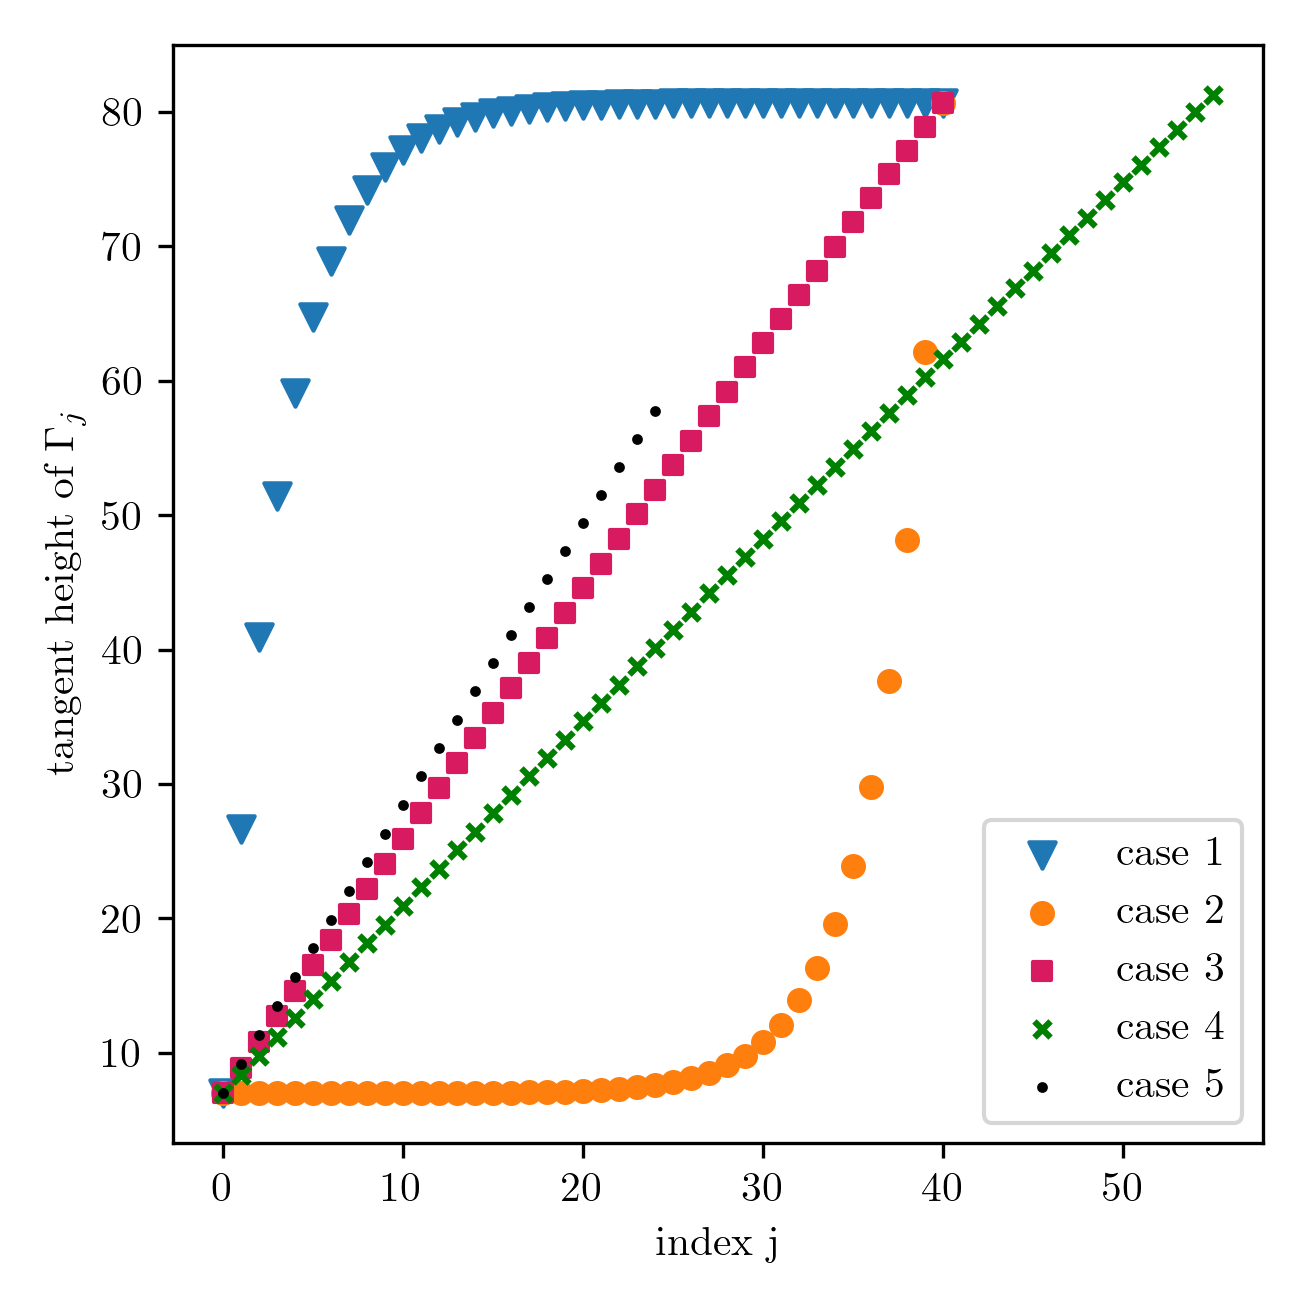
\includegraphics{MeasTangHeight.png}
	\caption[Tangent heights for different sequences of measurements.]{Tangent heights for five different sequences of measurements.}
	\label{fig:TangHCases}
\end{figure}
We test five different measurement strategies and plot the tangent heights in Fig.~\ref{fig:TangHCases}.
We either measure at equidistance-spaced pointing angles or collect more data from high signal regions at low altitudes or from low signal regions at high altitudes.
We visually asses how the singular values behave to determine which of the test cases is most effective.
More specifically, if the singular values decay fast and only few singular values are above a certain SNR the forward map is rather uninformative.
If the singular values decay less fast and more singular values are above a certain SNR the forward map is informative.
%\textcolor{red}{Another, they are multiplying like rabbits. Or flies. Which is more annoying?}
The measurement test case are:
\begin{itemize}
	\item \textbf{Case 1} includes 42 measurements between heights of $\approx7$km and $\approx83$km with pointing angles
	\begin{align*} 
		\phi_j  = \Bigg(\frac{-1}{1.25^{j-1}} + 1 \Bigg) \phi_{\text{max}} , \qquad  \text{for } j = 1, \dots, 42  \, .
	\end{align*}
	\item \textbf{Case 2} includes 42 measurements between heights of $\approx7$km and $\approx83$km with pointing angles
	\begin{align*} 
		\phi_j  = \frac{1.25 ^{j-1}}{ 1.25 ^{m-1}} 0.99 \phi_{\text{max}},  \qquad  \text{for } j = 1, \dots, 42\, .
	\end{align*}
	\item \textbf{Case 3} includes 42 measurements between heights of $\approx 7$km and $\approx 83$km with pointing accuracy $150 \text{arc sec}$ and pointing angles
	\begin{align*} 
		\phi_j  = (j-1) 150 \text{arc sec} ,  \qquad  \text{for } j = 1, \dots, 42\, .
	\end{align*}
	\item \textbf{Case 4} includes 83 measurements between heights of $\approx 7$km and $\approx83$km with pointing accuracy $77.5 \text{arc sec}$  and pointing angles
	\begin{align*} 
		\phi_j  =   (j-1) 77.5 \text{arc sec} ,  \qquad  \text{for } j = 1, \dots, 83\, .
	\end{align*}
	\item \textbf{Case 5} includes 30 measurements between heights of $\approx 7$km and $\approx 68$km with pointing accuracy $175  \text{arc sec}$ and pointing angles
	\begin{align*} 
		\phi_j  =  (j-1) 175 \text{arc sec} ,  \qquad  \text{for } j = 1, \dots, 30\, .
	\end{align*}
\end{itemize} 
%\textcolor{red}{why is this plot here before you defined the cases? That's not remotely OK.}

\begin{figure}[ht!]
	\centering
	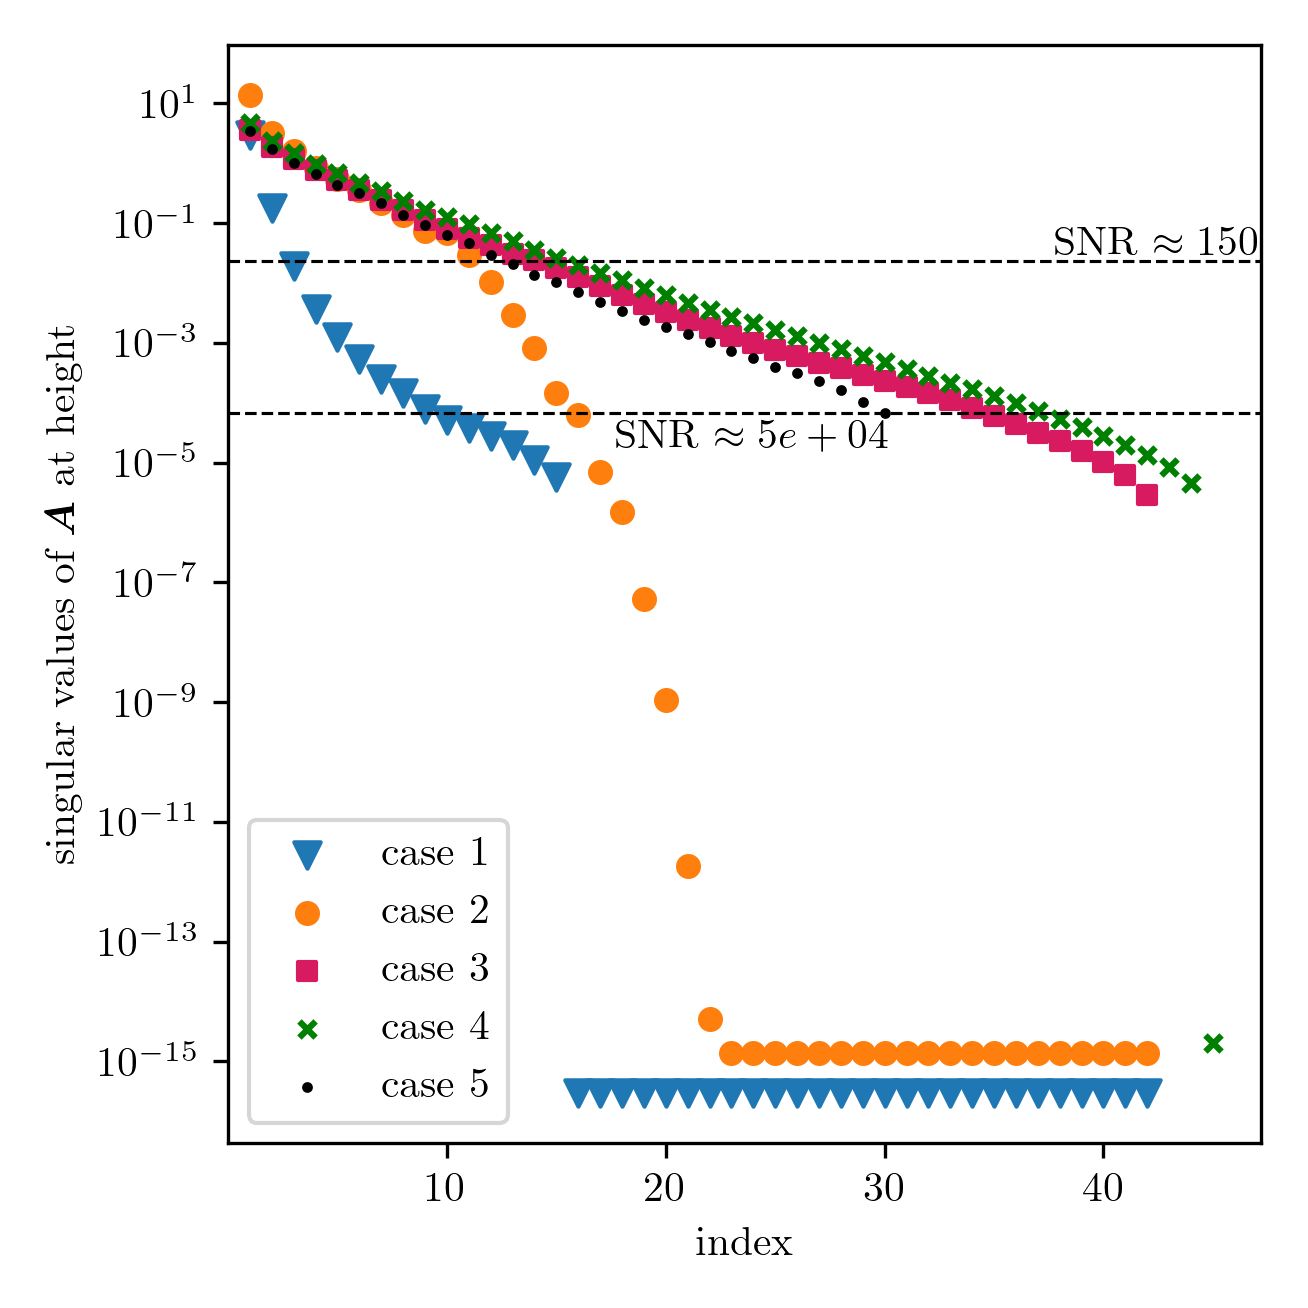
\includegraphics{SingValA.png}
	\caption[Singular values of linear forward model matrix for different sequences of measurements.]{Singular values of the forward model matrix for different sequences of measurements.
		The corresponding tangent heights of the test cases are plotted in Fig.~\ref{fig:TangHCases}. The dotted vertical line marks a SNR according to $\sigma_1$ of measurement case 5.}
	\label{fig:SingA}
\end{figure}
We start with case 3 in Fig.~\ref{fig:TangHCases} where measurements are spaced according to a pointing accuracy of $150\text{arc sec}$, given to us by the team of the University of New South Wales Canberra Space~\cite{CubeSatInternal}. \textcolor{red}{more sentence creep. }
The pointing accuracy determines how well the satellite can point in a certain direction and, hence the spacing in between two measurements.
The corresponding singular values are plotted in Fig.~\ref{fig:SingA}, of which the first 25 decrease linearly in log-space and about 10-15 singular values lie above the SNR. \textcolor{red}{where is this spacing? At the satellite? A spacing in time? On the planet Mars. Be specific. All the way through, you need to tighten up loose statements like this.}
In comparison, if we measure a lot of times in regions where the data is noise-dominated (high altitude), case 1, we do obtain more information since the singular values decrease rapidly.
\textcolor{red}{Oh come on, you are showing pictures of singular values without specifying exactly what the forward map and discretization is. That's not acceptable. If these are intended to be indicative, you need to be a damn site clearer about what they represent, and are trying to show.}
Measuring lots of times at low altitudes, where the data is informative, and less at higher altitudes, case 2, does not seem optimal either, as we observe one larger singular value, but the other singular values decrease faster compared to case 3.
Now consider case 4, where we double the number of measurements compared to case 3, we do get slightly larger singular values, but not so significantly that it would be worth the engineering effort required to achieve that.
The measurements with equidistance-spaced tangent height seem to be most effective. \textcolor{red}{why? Explain your reasoning. If you don't say something specific, quantitative, it's just waffle.}
By exploratory analysis, we find that we can tolerate a slightly larger distance between tangent heights (pointing accuracy of $175\text{arc sec}$) than required by~\cite{CubeSatInternal}, see case 5.
In that case, we also stop measuring when the signal is too noisy and decrease the number of measurements taken without losing crucial information.
We note that if one wanted to obtain all information provided by the forward model, we would need a signal-to-noise ratio of roughly $10^7$.

In principle, we show that it does not depend on how one measures; one cannot get more information by measuring more in regions where the information content is low or high.
\textcolor{red}{on the contrary - -you have just been arguing that it does matter. no, this makes sense if the goal is to reduce noise.}
This contradicts the current measurement setup on the AURA MLS~\cite{livesey2006retrieval}, which reports high noise in lower atmospheric regions, due to thermal radiation from the earth, and measures more in those regions.

%\textcolor{red}{oh no, I had hpped this section would be 'we' free.}
%\textcolor{red}{where do you explain why this SNR has a line here?,
%Were is the clear definition of these cases? I could not find it.}

\begin{figure}[ht!]
	\centering
	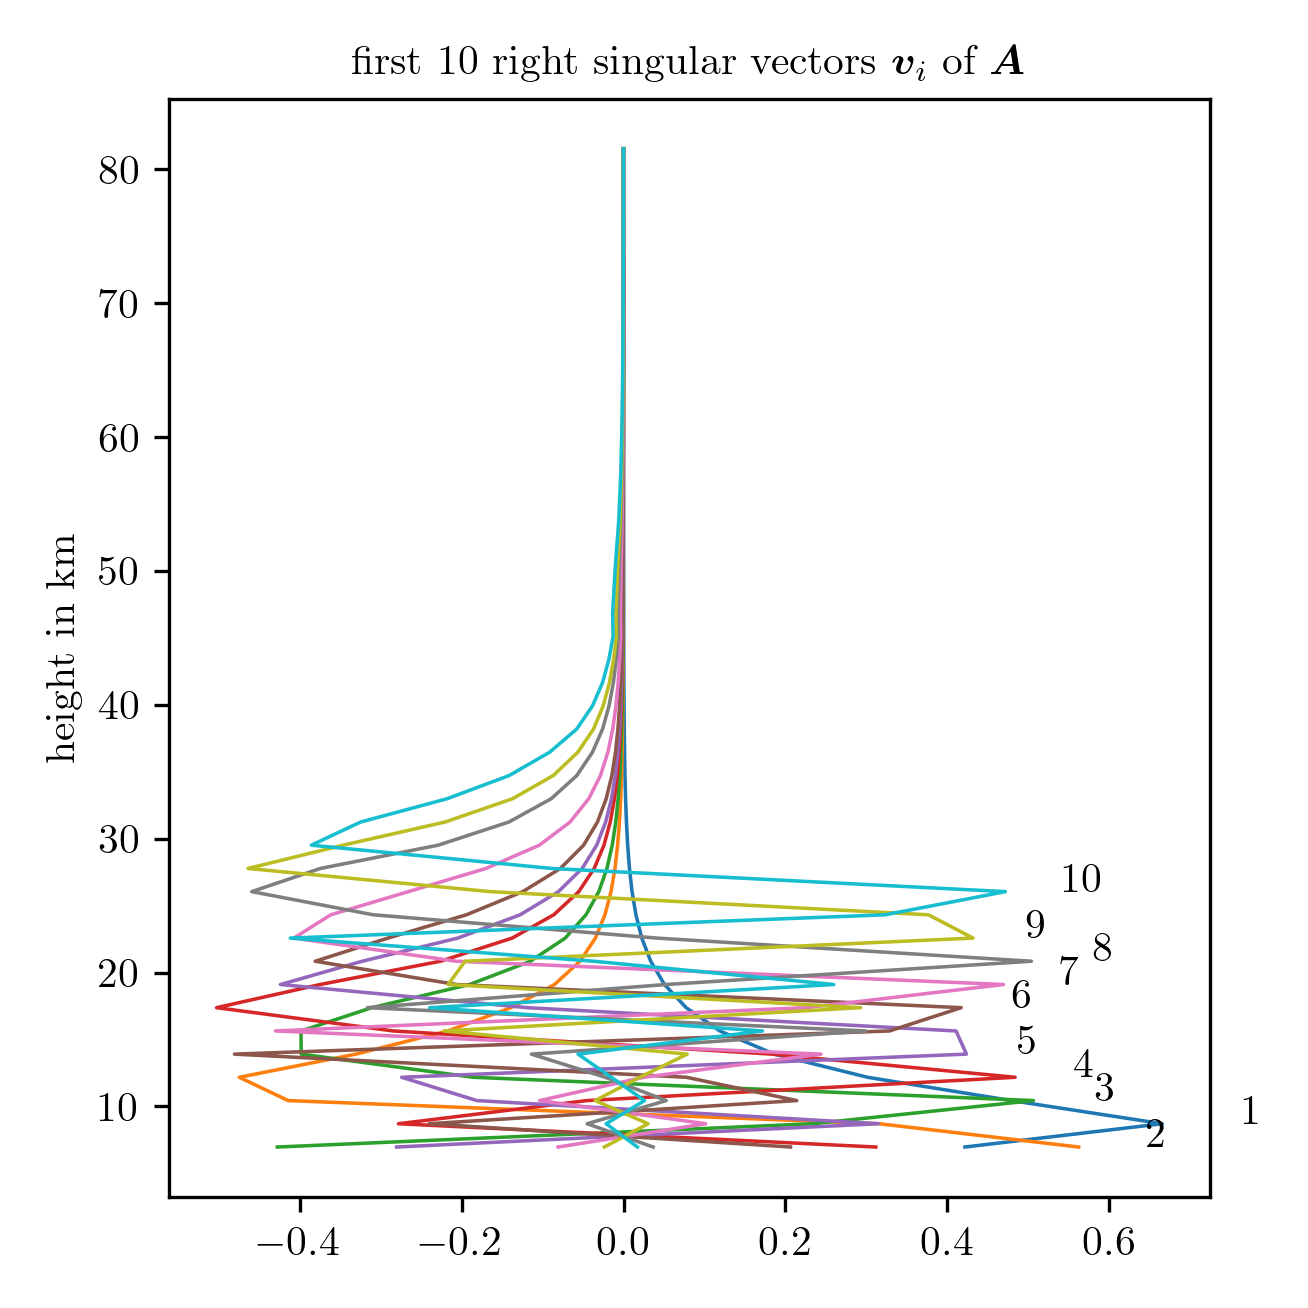
\includegraphics{SingVecA.png}
	\caption[First 10 right singular vectors of forward model.]{First 10 right singular vectors of the forward model matrix for measurements case 5 in Fig.~\ref{fig:TangHCases}. These singular vectors correspond to high singular values of the forward model in Fig.~\ref{fig:SingA}.}
	\label{fig:SingVecA}
\end{figure}
\begin{figure}[ht!]
	\centering
	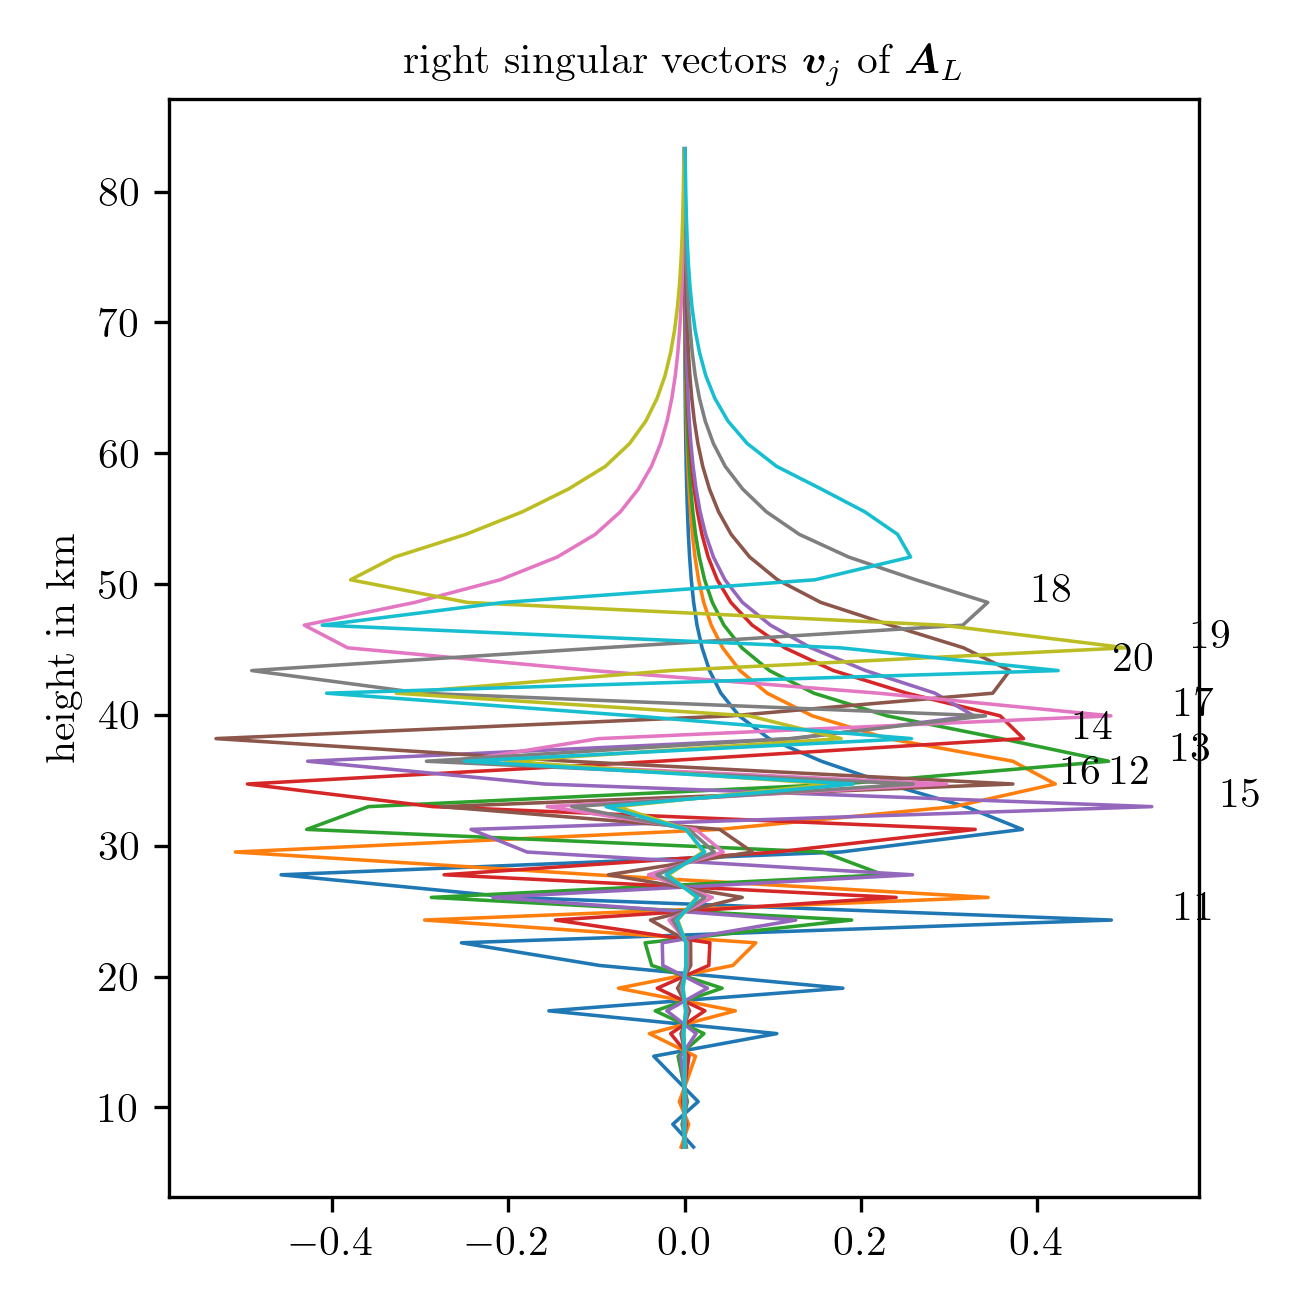
\includegraphics{MiddleVecA.png}
	\caption[Right singular vectors 11 to 19 of forward model.]{Right singular vectors with index $i = 11,\dots, 19$ of the forward model matrix for measurements case 5 in Fig.~\ref{fig:TangHCases}.
		These singular vectors correspond to singular values in Fig.~\ref{fig:SingA} where the noise level is similar to the data.}
	\label{fig:middleSpace}
\end{figure}
\begin{figure}[ht!]
	\centering
	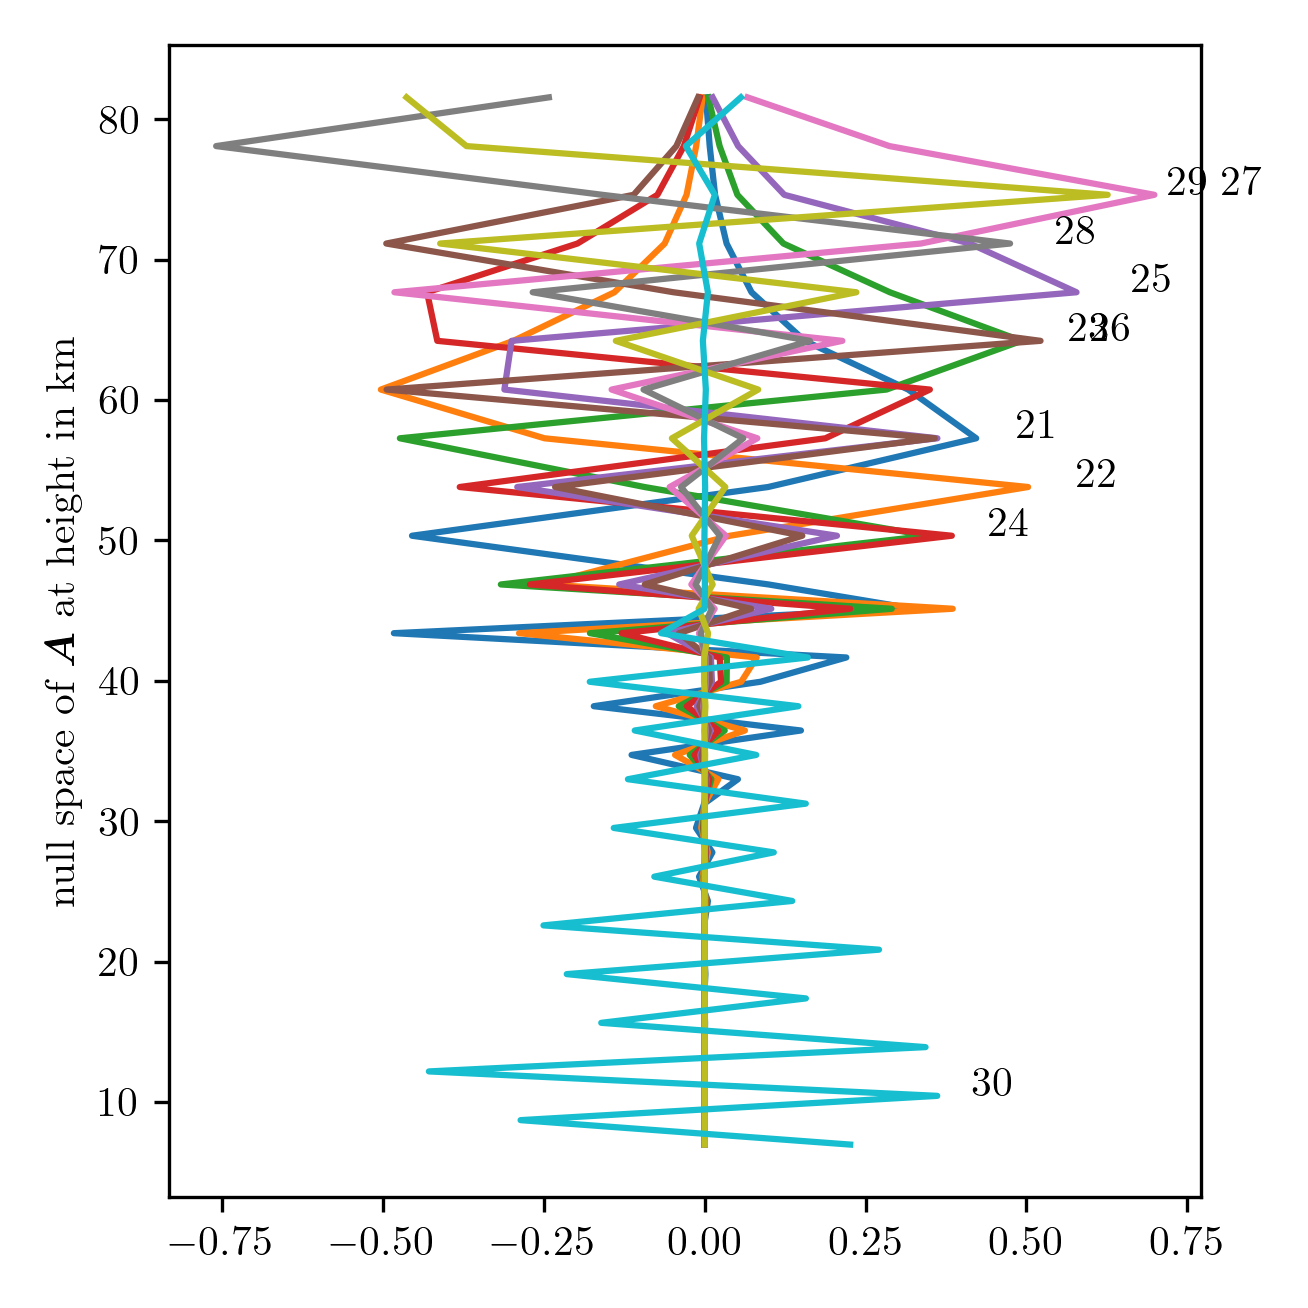
\includegraphics{NullVecA.png}
	\caption[Last 10 right singular vectors of forward model.]{Last 10 right singular vectors of the forward model matrix for measurements case 5 in Fig.~\ref{fig:TangHCases}. These singular vectors correspond to small singular values of the forward model in Fig.~\ref{fig:SingA} where the data is noise-dominated.}
	\label{fig:nullSpace}
\end{figure}
The parameter space of $\bm{A}_L$ spanned by the first 10 singular values represent only vlaues in the lower atmosheric regions.
Consequently, we proceed with case 5 and plot the right singular vectors of the forward model versus height in the atmosphere to see where our model is most informative, or which structures of the parameter space are picked up by the model.
The first 10 right singular vectors, in Fig.~\ref{fig:SingVecA}, corresponding to the 10 largest singular values, pick up parameter structures in lower atmospheric regions.
So we can assume that, given some data, we will be able to provide good reconstructions of the parameter in lower altitudes. \textcolor{red}{too colloquial. One picks up rubbish, not sure what it means in this context.}
Next, we plot the right singular vectors corresponding to the singular values $\sigma_j$ for $j = 11, \dots, 20$ in Fig. \ref{fig:middleSpace}, where the noise starts to dominate the data.
These singular values lie in regions around the SNR, see Fig.~\ref{fig:SingA}, and pick up values in the middle of the atmosphere. \textcolor{red}{ditto}
Consequently, we expect a higher uncertainty of reconstructed parameter values in the middle atmospheric regions.
The singular vectors corresponding to the last 10 singular values pick up parameter structures in higher altitudes, but since the singular values are very small, we will not be able to retrieve those structures.
More specifically, the retrieved parameter values at higher altitudes will be mostly determined by the prior or, in the case of regularisation, by the regulariser~\cite{tan2016LecNot}.

The difference in between tangent heights is between 2.05km and 2.17km.
 \textcolor{red}{Actually, you should calculate this from the MIPAS specifications, or similar. It claims 1-3km resolution, presumably at a distance of 500km. So, what's that in arc seconds? It's also related to your vertical discretization, or, more to the point, your vertical discretization is determined by this.}
 
\begin{figure}[th!]
	\centering
	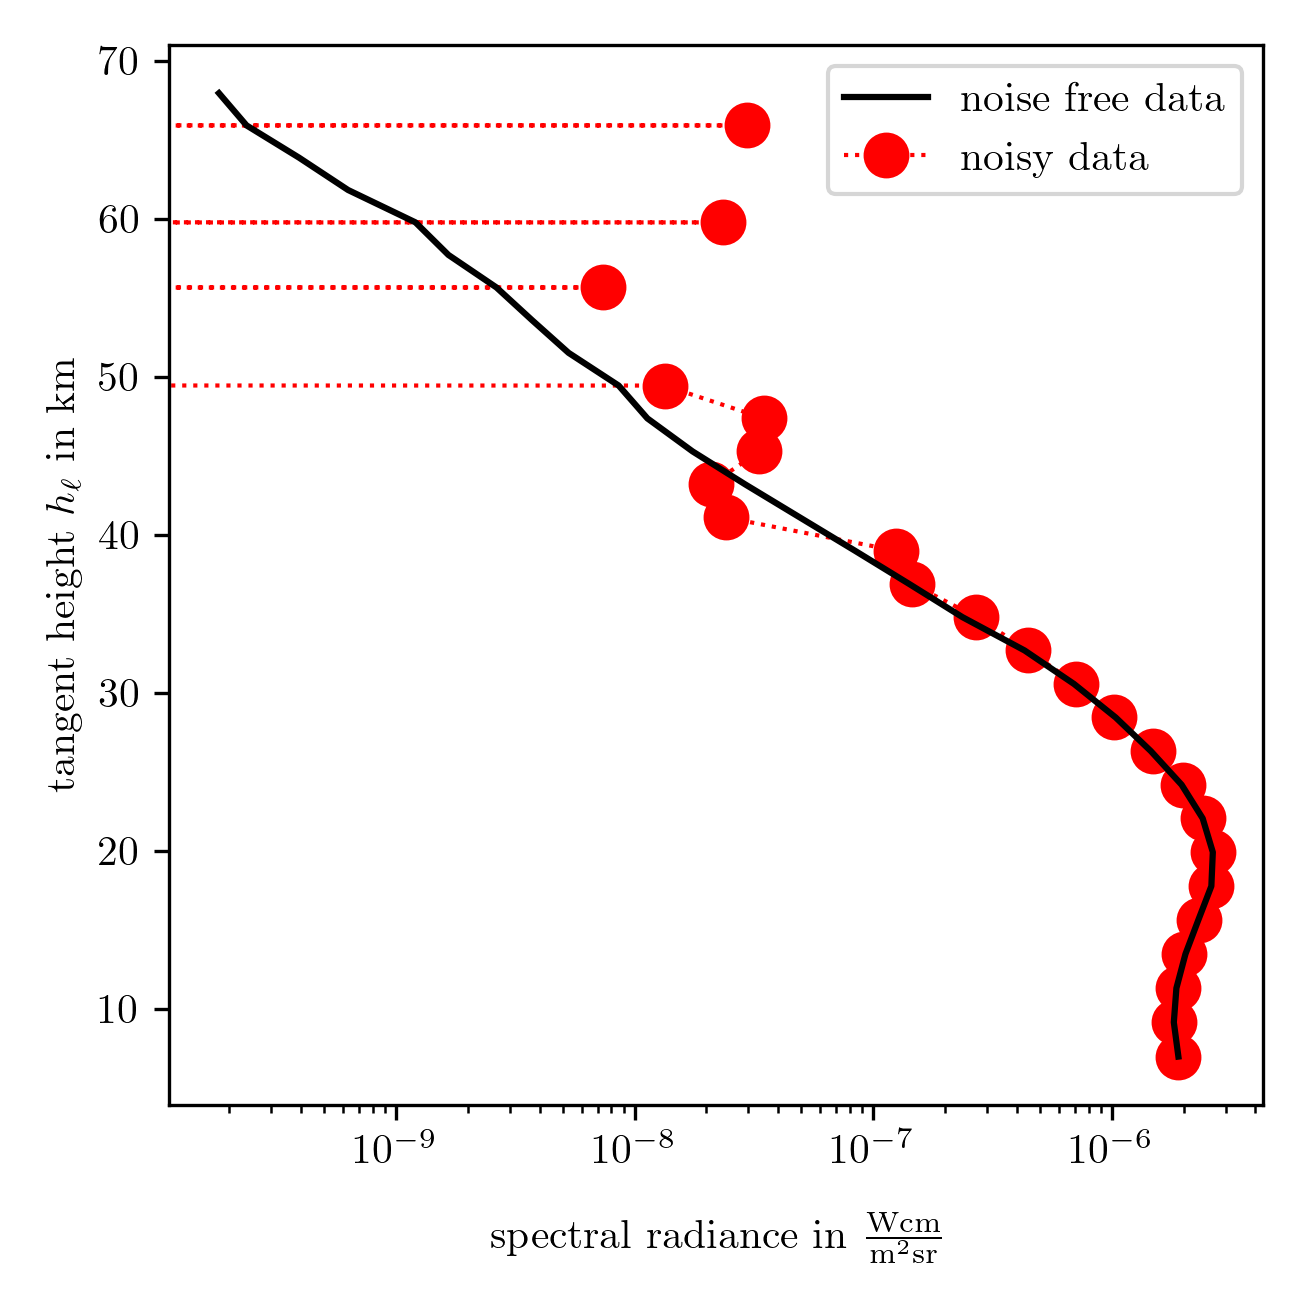
\includegraphics{DataPlot.png}
	\caption[Logarithmic plot of data points at different tangent height.]{Logarithmic plot of data points at different tangent height. Note that negative values are not plotted, and noise is dominating at higher altitudes.}
	\label{fig:DataPlot}
\end{figure}
We plot the data in Fig.~\ref{fig:DataPlot}, which is noise-dominated in higher altitudes and hence not sensitive to structures in the higher atmospheric regions.
Now, given the data, we like to determine the posterior distributions over ozone $\bm{x}$, pressure $\bm{p}$ and temperature $\bm{T}$.
\clearpage

Then we can compute a data vector $\bm{y} = \bm{A}(\bm{x}) + \bm{\eta} $, with $m = 30$ measurements determined by the satellite pointing accuracy of $175\text{arc sec}$ (see case 5 in Fig.~\ref{fig:TangHCases}), according to the RTE as in Eq.~\ref{eq:RTE} and Eq.~\ref{eq:absRTE} using the trapezoidal integration rule.
We assume an atmosphere between $h_{L,1}=7$km and $h_{L,n} = 83.3$km with $n = 45$ equidistant layers (see Fig.~\ref{fig:LIMB}).
The height value $h_{L,i}$ for each layer $i = 1,\dots, n$ is defined by the pressure values from~\cite{MLSdata} and the hydrostatic equilibrium equation, see Eq.~\ref{eq:hydr}.
We target ozone at a frequency of 235.71GHz, which lies within the region where the MLS observes ozone~\cite{livesey2008ozonecarbonmono, waters2006earth}.
The corresponding wave number is $\nu = 7.86\text{cm}^{-1}$.
We calculate the absorption constant $k(\nu,T)$ as in Eq.~\ref{eq:absRTE}, following the high resolution transmission (HITRAN) database~\cite{gordon2022hitran2020}, which provides the line intensity $L(\nu,T_{\text{ref}})$ for the isotopologue $\prescript{16}{}{\text{O}}_3$ with the AFGL Code 666.
%This gives us a non-linear forward model matrix $\bm{A}_{NL} = \bm{A}(\bm{x}, \bm{p}, \bm{T}) \in \mathbb{R}^{m \times n}$, where $\bm{x}\in \mathbb{R}^{n}$ is vector related to the ozone VMR, $\bm{p}\in \mathbb{R}^{n}$ is the vector describing the pressure values and $\bm{T}\in \mathbb{R}^{n}$ the temperature values.
Lastly, we add independent and identically-distributed Gaussian noise $\bm{\eta} \sim \mathcal{N}(0,\gamma^{-1} \bm{I})$ so that the $\text{SNR}=150$ (see Eq.~\ref{eq:SNR}) similar to~\cite{Froidevaux2008snrozone}, where a signal with a maximal spectral intensity of around $100\text{K}$ and a noise range of $0.4$ to $1.6\text{K}$ is reported.
We note that the methods used in this thesis will work with different SNRs or other frequencies.
\chapter{Linear Bayesian vs. Regularisation -- Ozone}
\label{ch:LinVsReg}
\thispagestyle{empty}

In this Chapter, we guide the reader through the process of setting up a hierarchical Bayesian framework, establishing a choice of prior distributions, and using a DAG to visualise conditional dependencies between hyper-parameters and parameters.
Applying the MTC scheme the marginal and then full conditional posterior distributions are explicitly formulated.
Here this inverse problem is treated as a linear inverse problem by neglecting the absorption term in the RTE (see Eq.~\ref{eq:RTE}).
A Metropolis within Gibbs sampler and a TT approximation are utilised to characterise the marginal posterior.
Then the mean and the covariance matrix of the posterior distribution for ozone are calculated and compared to a regularisation approach.


\section{Hierarchical Bayesian Framework}
\label{sec:BayModelO3}
\begin{figure}[htb!]
	\centering
	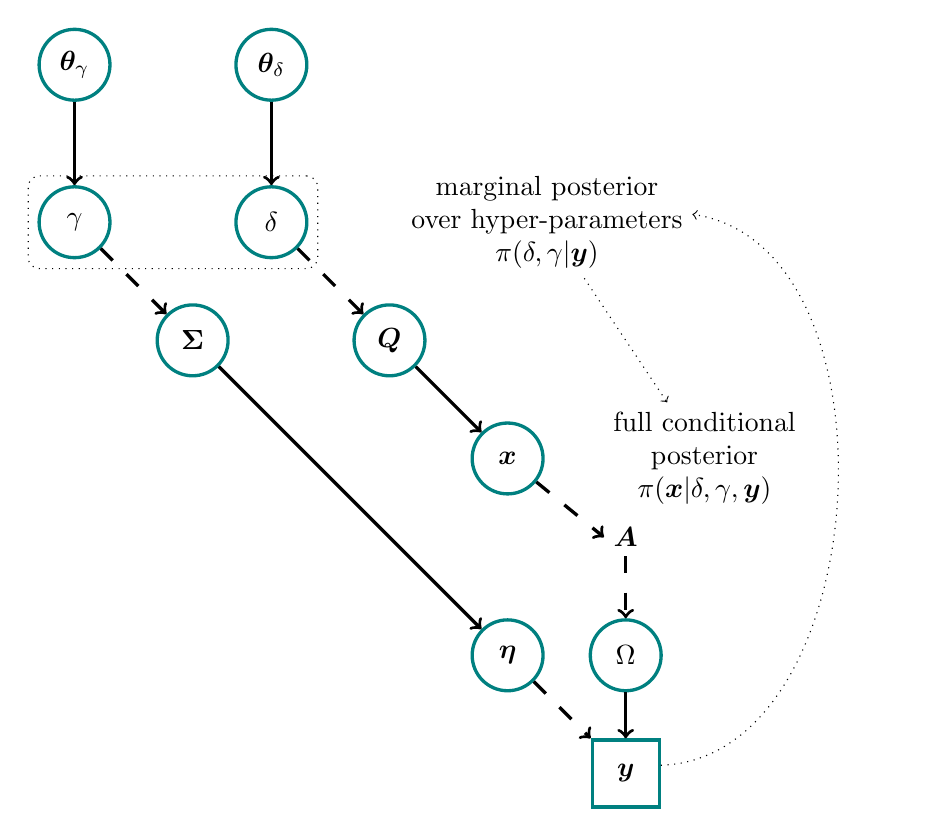
\begin{tikzpicture}
		%box/.style = {draw, thick, minimum width=2.5cm, minimum height=1cm},
		every edge/.style = {draw, -latex, thick} % <---
		\node[roundnode2] at (-4,6.5) (Q)     {$\bm{Q}$};
		\node[roundnode2] at (-2.5,5) (x)     {$\bm{x}$};
		\node[align=center] at (-1,4) (A)    {$\bm{A}$};
		\node[roundnode2] at (-1,2.5) (u)    {$\Omega$};
		\node[rectnode] at (-1,1) (y)    {$\bm{y}$};
		\node[roundnode2] at (-2.5,2.5) (e)    {$\bm{\eta}$};
		\node[roundnode2] at (-6.5,6.5) (S)    {$\bm{\Sigma}$};
		\node[roundnode2] at (-8,8) (s)    {$\gamma$};
		\node[roundnode2] at (-5.5,8) (d)    {$\delta$};
		
		\node[roundnode2] at (-8,10) (shyp)    {$\bm{\theta}_{\gamma}$};
		\node[roundnode2] at (-5.5,10) (dhyp)    {$\bm{\theta}_{\delta}$};
		%Lines
		\draw[->, very thick] (S) -- (e);
		\draw[->, mydotted, very thick] (s) -- (S);
		\draw[->, mydotted, very thick] (e) -- (y);
		\draw[->, very thick] (u.south) -- (y);
		\draw[->, mydotted, very thick] (A) -- (u);
		\draw[->, mydotted,  very thick] (x) -- (A.west);
		\draw[->, very thick] (shyp) -- (s);
		\draw[->, very thick] (dhyp) -- (d);
		
		
		\draw[->, mydotted, very thick] (d) -- (Q); 
		
		\draw[->, very thick] (Q) -- (x); 
		%\node[align=center] at (0,4) (f3) {$= \bm{A}$};
		%\node[align=center] at (0.25,3.95) (f3) {$\approx \bm{M A}_L$};
		\node[align =center] at (-2,8) (T1) {marginal posterior \\ over hyper-parameters \\ $\pi(\delta,\gamma  | \bm{y})$};
		\node[align =center] at (0,5) (T2) {full conditional \\ posterior \\ $\pi( \bm{x} | \delta,\gamma, \bm{y})$ };
		
		%\node[align =center] at (-2.5,10) (T3) {hyper-prior distributions \\ $\pi( \delta, \gamma)$ };
		
		\node[fit=(s)(d),draw,dotted,black, rounded corners] {};
		\draw[->,dotted] (y) edge[bend right=85] (T1);  
		\draw[->,dotted] (T1) -- (T2); 
		
	\end{tikzpicture} 
	\caption[Directed acyclic graph for ozone retrieval and MTC scheme.]{DAG for visualisation of hierarchical modelling and measuring process of ozone, including the MTC scheme. The hyper-parameter $\gamma$ deterministically (dotted line) sets the noise covariance $\bm{\Sigma} = \gamma^{-1}\bm{I}$ and hence the random (solid line) noise vector $\bm{\eta} \sim \mathcal{N}(0, \gamma^{-1}\bm{I})$.
		The hyper-parameter $\delta$ determines (dotted line) the prior precision matrix $\bm{Q} = \delta \bm{L}$ for the normally distributed (solid line) prior $\bm{x}| \delta \sim \mathcal{N}(0, \delta \bm{L})$, where $\bm{L}$ is a graph Laplacian, see Eq.~\ref{eq:GLapl}.
		The hyper-prior distributions (solid line) $\pi(\delta, \gamma)$ are defined by $\bm{\theta}_{\gamma}$ and $\bm{\theta}_{\delta}$.
		Through a linear forward model $\bm{A}$, we generate a space of all measurable noise-free data $\bm{A}\bm{x}$ from which we randomly observe a data set $\bm{y}$ including some added noise $\bm{\eta}$.
		Within the MTC scheme, we evaluate the marginal posterior over the hyper-parameters $\pi(\gamma, \delta | \bm{y})$ first and then the full conditional posterior $\pi(\bm{x}|\delta,\gamma,\bm{y})$. This breaks the correlation structure of $\bm{x}$ and $\delta$ and $\gamma$, and allows us to evaluate the marginal posterior independent of $\bm{x}$.}
	\label{fig:DAGO3}
\end{figure}
In this section, we set up the hierarchically-ordered linear-Gaussian Bayesian framework to determine the ozone posterior distribution, conditioned on ground truth temperature and pressure.
For now the forward model matrix is defined as $\bm{A} \coloneqq \bm{A}_L$ and the distributions that define the hierarchical Bayesian model are:
\begin{subequations}
		\label{eq:O3BayMode}
	\begin{align}
		\bm{y} |  \bm{x},\gamma,\delta  &\sim \mathcal{N}(\bm{A} \, \bm{x}, \gamma^{-1} \bm{I}) \label{eq:likelihoodAppl} \\
		\bm{x}| \delta  &\sim \mathcal{N}(\bm{0}, (\delta \bm{L})^{-1} ) \label{eq:priorXAppl} \\
		\delta  &\sim \Gamma(\alpha_{\delta}, \beta_{\delta})\label{eq:priorDelAppl} \\
		\gamma  &\sim \Gamma(\alpha_{\gamma}, \beta_{\gamma})\label{eq:priorGamAppl} \, .
	\end{align} 
\end{subequations}
Assuming Gaussian noise $\bm{\eta} \sim \mathcal{N}(0, \gamma^{-1} \bm{I})$, the likelihood function is a normal distribution with mean $\bm{A} \bm{x}$ and covariance matrix $\gamma^{-1} \bm{I}$.
We define a normal prior-distribution $\pi(\bm{x}|\delta)$ with zero mean and precision matrix $\delta \bm{L}$, where $\delta$ is a smoothness hyper-parameter and $\bm{L}$ is a discrete approximation to the second derivate operator (see Eq.~\ref{eq:GLapl}).
Here the hyper-prior distributions $\pi(\delta)$ and $\pi(\gamma)$ are Gamma distributions with shape $\alpha$ and rate $\beta$.

We can visualise this hierarchical structure and the conditional dependencies between hyper-parameters and parameters through a DAG, as in Fig.~\ref{fig:DAGO3}.
The hyper-parameter $\gamma$ sets the noise covariance deterministically (dotted line), but is itself statistically (solid line) defined by the hyper-prior distribution $\pi(\gamma)$.
This is a Gamma distribution, where $\bm{\theta}_{\gamma}$ determines the shape and rate of $\pi(\gamma)$.
Similarly $\bm{\theta}_{\delta}$ defines $\pi(\delta)$, where $\delta$ accounts for smoothness of the ozone profile and sets the prior precision $\bm{Q}(\delta)$.
Then $\bm{A}\bm{x}$ determines the space of all measurable noise-free data sets $\Omega$ through the linear forward model, from which we observe a data set $\bm{y}$ including some noise $\bm{\eta}$.
Given that data, we ``reverse the arrows'' to determine the posterior distribution $\pi(\bm{x}, \bm{\theta}|\bm{y})$ over the parameter $\bm{x}$ and the hyper-parameters $\bm{\theta}$.
%Since noise is a random process with a defined distribution, the posterior distribution $\pi(\bm{x}|\bm{y})$ is well defined.
Usually, due to underlying correlation structures between the parameter and the hyper-parameters, evaluating this posterior poses a signifiant challenge.
The MTC scheme breaks this correlation and provides the marginal posterior $\pi(\delta, \gamma | \bm{y})$ first and then the full conditional posterior $\pi(\bm{x}|\delta, \gamma,\bm{y})$.
%Since the forward model described in Ch. \ref{ch:formodel} is weakly non-linear we will set up a linear Bayesian hierarchical framework first based on the linear forward model $\bm{A}_L$ and then later the approximated version $\bm{A}_{NL}\bm{M} \bm{A}_L$.
%Furthermore, the noise is normally distributed, so we establish a linear-Gaussian Bayesian hierarchical framework, aiming to recover an ozone profile and a pressure over temperature profile.
%In doing so, we first draw a directed acyclic graph (DAG) to visualise the measurement and modelling process and determine hyper-parameters and correlations between parameters.
%Then we define prior distributions over all parameters as well as a likelihood function so that we can formulate the posterior distribution.

%In this section, we choose the prior distributions and describe the approach to evaluate the posterior distribution for ozone $\pi(\delta, \gamma, \bm{x}|\bm{y})$, including the noise hyper-parameter $\gamma$.
% we define a linear-Gaussian Bayesian hierarchical model, see Sec. \ref{subsec:LinBay},
%\begin{subequations}
%	\begin{align}
	%		\bm{y} |  \bm{x}, \gamma &\sim \mathcal{N}(\bm{A} \bm{x}, \gamma^{-1} \bm{I}) \label{eq:likelihood} \\
	%		\bm{x} |  \delta &\sim \mathcal{N}(\bm{0}, (\delta \bm{L})^{-1}) \label{eq:xPrior} \\
	%		\delta, \gamma &\sim \pi(\delta, \gamma) \label{eq:gammaPrior},
	%	\end{align}
%	\label{eq:O3BayMode}
%\end{subequations}
%with a normally distributed likelihood $\pi(\bm{y} |  \bm{x}, \gamma)$ including the forward model matrix $\bm{A}$ and prior distributions $\pi(\bm{x} |  \delta)$ and $\pi(\delta, \gamma)$, the noise covariance matrix $\gamma^{-1} \bm{I}$, the prior precision matrix $\delta \bm{L}$ and the prior mean set to zero, as in ~\cite{fox2016fast}.
%The chosen Bayesian model is very similar to the regularisation approach, since we like to show that we receive much more meaningful results compared to a single regularisation solution.

\subsection{Prior Modelling}
\label{subsec:PriorModelO3}
Completing this Bayesian framework one has to define prior distributions over the hyper-parameters and parameters.
Ideally, we define the prior distributions as uninformative as possible, and include functional dependencies and physical properties.

By choosing a normally distributed prior $\pi(\bm{x}|\delta)$ with zero mean and no other restrictions, it is clear that our model does not take into account that ozone values cannot be negative.
As already mentioned, we set the precision matrix of that prior distribution to
\begin{align}
	\delta \bm{L} =
	\delta
	\begin{bmatrix}
		2 & -1 & & &  \\
		-1 & 2 & -1 & &   \\
		& \ddots & \ddots & \ddots &\\ 
		& & -1 & 2 & -1  \\
		& & & -1 & 2 
	\end{bmatrix} 
	\label{eq:GLapl} 
\end{align}
which is a discrete approximation to the second derivate operator with Dirichlet boundary condition and defines a 1-dimensional Graph Laplacian as in~\cite{wang2015graphs, fox2016fast}.
This matrix will also act as the regulariser later in Sec.~\ref{sec:SolByReg}.
We reduce the dimension of $\bm{x}$ from $45$ to $34$ by discarding every second ozone VMR over a height of $\approx47$km.
Doing that, while not changing $\bm{L}$, we effectively induce a larger correlation between points at higher altitude.
We plot the corresponding prior ozone profiles according to $\bm{x}\sim \mathcal{N}(0, (\delta \bm{L})^{-1})$ in Fig.~\ref{fig:O3Prior}.

For $\delta$ and $\gamma$ we pick relatively uninformative gamma distributions so that $\gamma \sim \mathcal{T}(\bm{\theta_{\gamma}}) \propto \gamma^{\alpha_\gamma -1 } \exp{( -\beta_\gamma \gamma) } $ and $\delta \sim \mathcal{T}(\bm{\theta_{\delta}})$, where $\bm{\theta_{\gamma}} = \{  \alpha_\gamma, \beta_\gamma\}  = \{ \alpha_\delta ,\beta_\delta\} = \bm{\theta_{\delta}} = (1,10^{-35})$ (see Fig.~\ref{fig:MargPostHistTT}) similar to \cite{fox2016fast}.
Because of those gamma distributions, $\pi(\gamma | \lambda, \bm{y}) \sim \mathcal{T}(\cdot)$ is a gamma distribution with $\lambda = \delta / \gamma $ and easy to sample from.
This advantageous when using the Metropolis within Gibbs algorithm, as in Sec.~\ref{subsec:MWG}, to sample from the marginal posterior distribution $\pi(\delta, \gamma | \bm{y})$.

\section{Posterior Distribution}
\label{sec:FirstO3Post}
As explained in Sec.~\ref{subsec:TheoMTC}, we factorise the posterior
\begin{align}
	\pi( \bm{x}, \delta, \gamma| \bm{y}) \propto \pi(\bm{y}| \bm{x},\delta,\gamma) \pi( \bm{x},  \delta,\gamma)
\end{align}
into 
\begin{align}
	\pi( \bm{x},  \delta,\gamma| \bm{y}) =\pi( \bm{x}| \delta,\gamma, \bm{y})\pi( \delta,\gamma | \bm{y})
\end{align}
the marginal posterior $\pi(\delta ,\gamma| \bm{y})$ and full conditional posterior $\pi( \bm{x}| \delta,\gamma, \bm{y})$ (see Eq.~\ref{eq:MTC}).
%Fox and Norton call this method the marginal and then conditional method (MTC) \cite{fox2016fast}, where we break the correlation structure between $\bm{x}$ and $\gamma, \delta$ as illustrated in Fig. \ref{fig:RueHeld} by marginalising over $\bm{x}$.
As discussed in Sec.~\ref{subsec:LinBay}, for the linear-Gaussian case, $\bm{x}$ cancels in the marginal posterior over the hyper-parameters~\cite{fox2016fast}.
Following the MTC scheme, we characterise the marginal posterior first and then the full conditional posterior.

\subsection{Marginal Posterior}
\label{subsec:FirstMargPost}
Consequently, for the hierarchical model specified in Eq.~\ref{eq:O3BayMode}, the marginal posterior distribution over the hyper-parameters is given by
\begin{align}
	\pi( \lambda,\gamma  | \bm{y}) \propto &  \lambda^{n/2 + \alpha_{\delta}-1} \gamma^{m/2 + \alpha_{\delta} + \alpha_{\gamma}-1}   \exp{ \Bigl\{ - \frac{1}{2} g ( \lambda) - \frac{\gamma}{2} f ( \lambda) - \beta_{\delta} \lambda  \gamma - \beta_{\gamma} \gamma \Bigr\}},
	\label{eq:MargPostAppl}
\end{align}
with the introduced regularisation parameter $\lambda = \delta / \gamma$, and
\begin{subequations}
	\begin{align}
		&f ( \lambda) = \bm{y}^T \bm{y} - (\bm{A}^T \bm{y})^T (\bm{A}^T  \bm{A} + \lambda \bm{L})^{-1} (\bm{A}^T \bm{y})  \label{eq:fAppl} \, ,  \\
		&\text{and } g(\lambda) = \log \det (\bm{A}^T  \bm{A} + \lambda \bm{L}) \label{eq:gAppl} \, .
	\end{align}
\end{subequations}
Note that when changing variables from $\delta = \lambda \gamma$ to $\lambda$ the hyper-prior distribution changes to $\pi(\lambda) \propto \lambda^{\alpha_{\delta}-1} \gamma^{\alpha_{\delta}} \exp{(- \beta_{\delta} \lambda  \gamma)} $, due to $\text{d}\delta / \text{d} \lambda = \gamma$.
\begin{figure}[th!]
	\centering
	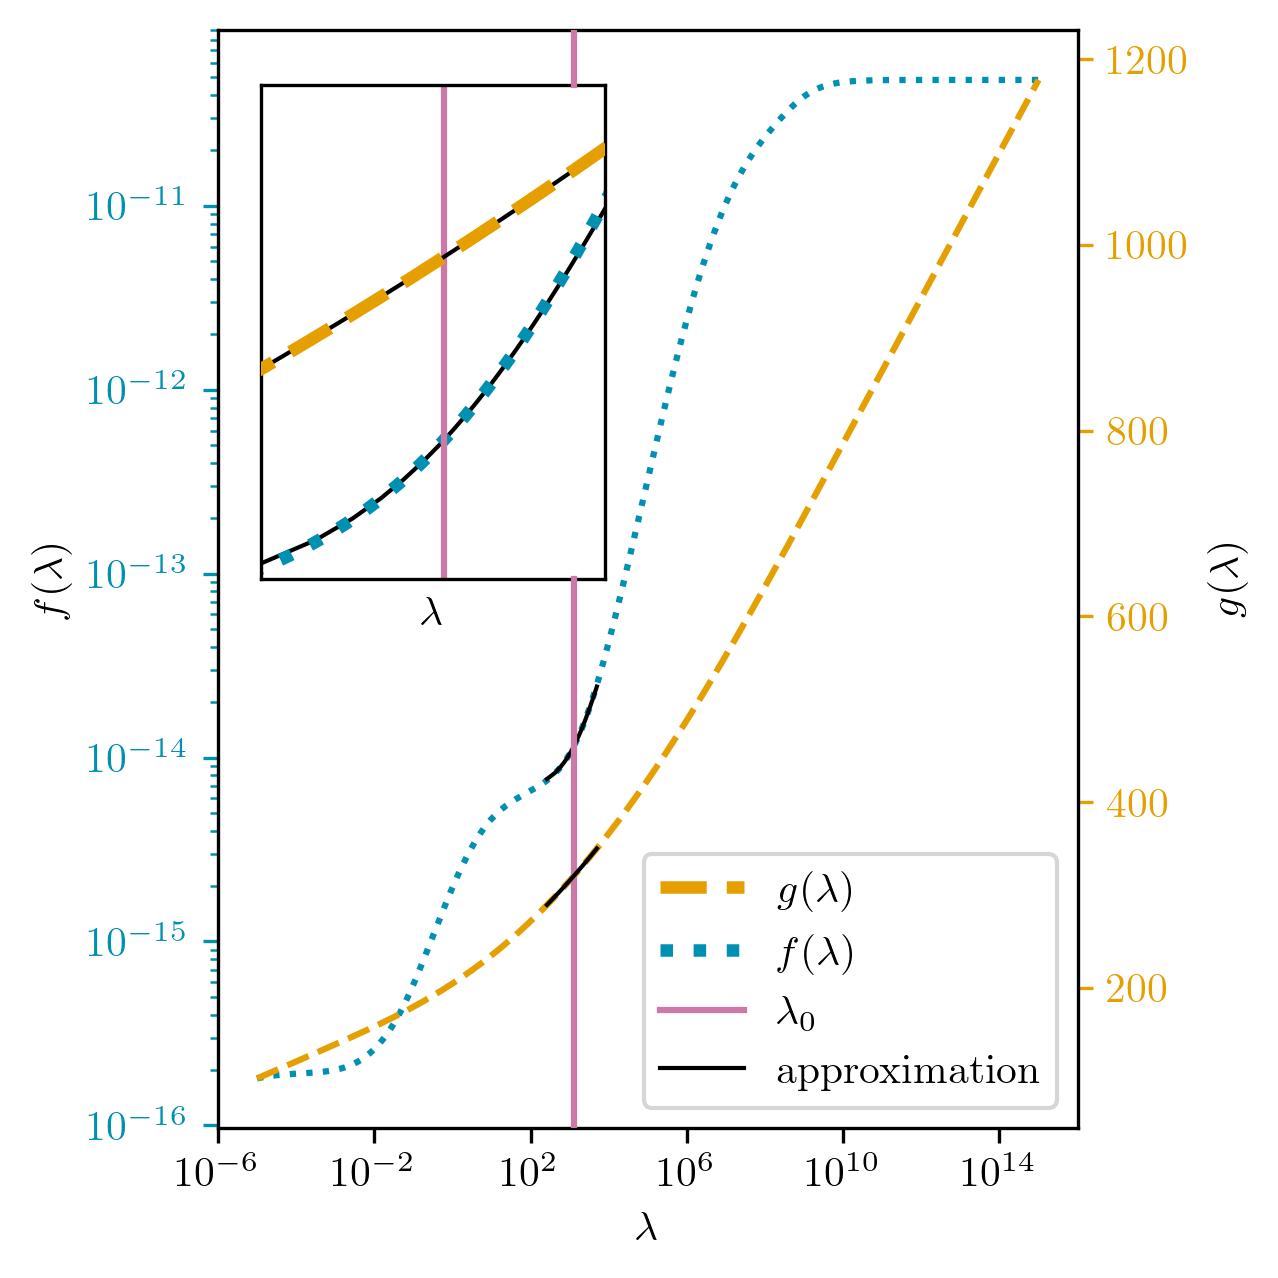
\includegraphics{f_and_g_phd.png}
	\caption[Functions $f(\lambda)$ and $g(\lambda)$ of 2D marginal posterior.]{Functions $f(\lambda)$ and $g(\lambda)$ from the marginal posterior in Eq.~\ref{eq:MargPostAppl} for a wide range of $\lambda = \delta / \gamma$. We plot the approximations (see Eq.~\ref{eq:fAprox} and Eq.~\ref{eq:gAprox}) in black around the mode of the marginal posterior (vertical line) for the sampling range of $\lambda$ within the MWG algorithm.}
	\label{fig:fandg}
\end{figure}
For each evaluation of the marginal posterior most of the computational effort lies in the calculation of $f(\lambda)$ and $g(\lambda)$.
Obtaining the Cholesky decomposition $\bm{A}^T  \bm{A} + \lambda \bm{L} = \bm{C}_{\lambda} \bm{C}_{\lambda}^T$ via \texttt{numpy.linalg.cholesky} immediately gives $g(\lambda) = 2 \sum \log \text{diag}(\bm{C}_{\lambda}) $.
Additionally this Cholesky decomposition is used to calculate $(\bm{A}^T  \bm{A} + \lambda \bm{L})^{-1} (\bm{A}^T \bm{y})$ as in $f(\lambda)$ via the Python function \texttt{scipy.linalg.cho\_solve}.
In  Fig.~\ref{fig:fandg} we see that $f(\lambda)$ and $g(\lambda)$ are well behaved within the region of interest.
Because of this, we approximate $\tilde{g}(\lambda) \approx g(\lambda)$ with a linear approximation in $\lambda$ log-space and $f(\lambda) \approx \tilde{f}(\lambda)$ with a Taylor series around the mode $\lambda_0$ of $\pi(\lambda, \gamma | \bm{y})$.
The Taylor series coefficient of $f(\lambda)$ is given by
\begin{align}
	f^{(r)}& (\lambda_0)= (-1)^{r+1} (\bm{A}^T \bm{y})^T (\bm{B}_0^{-1} \bm{L})^r \bm{B}_0^{-1} \bm{A}_L^T \bm{y} \label{eq:ftay} 
\end{align} 
with $\bm{B}_0 = \bm{A}^T  \bm{A} + \lambda_0 \bm{L}$.
Usually a Taylor series includes a factor $(r!)^{-1}$, which in this case cancels~\cite{fox2016fast} so that $f(\lambda)$ is approximated as 
\begin{align}
		\tilde{f} ( \lambda) = \sum^{\infty}_{r=0} 	f^{(r)}(\lambda_0) (\lambda-\lambda_0)^r  \label{eq:fAprox} \, . 
\end{align}
By exploratory analysis we find that the approximation
\begin{align}
 \tilde{g}(\lambda)=  g(\lambda_{0}) + (\log{\lambda} - \log{\lambda_{0}})  \frac{ g(1.25\lambda_{0}) - g(0.75\lambda_{0}) }{\log{1.25\lambda_{0}} - \log{0.75\lambda_{0}} }  \label{eq:gAprox} \, 
\end{align}
is sufficient.
Note that $g(\lambda)$ can be approximated with a Taylor series as well (see~\cite{fox2016fast}).
We plot the function $f(\lambda)$ and $g(\lambda)$ and their approximations in Fig.~\ref{fig:fandg} and elaborate on the approximation errors in the section below.

\subsubsection{Error due to approximation of f and g}
To assess the approximation error, we lay a 100-point grid over the sampling region in each dimension and compare the approximations of $f(\lambda)$, $g(\lambda)$ and $\pi(\lambda, \gamma | \bm{y})$ with their true function values.

Compared to a 2nd, 3-rd or 4-th order Taylor approximation, the 1-st order Taylor approximation of $f(\lambda)$ gives the smallest relative RMS error of $\approx 9 \%$ for $\lambda = [ 10^{-5}, 8 \times 10^{-4}]$ (TT grid) and a maximum absolute error of $\approx 3 \times 10^{-16}$.
Additionally, the linear approximation of $g(\lambda)$ has a relative RMS of $\approx 3\%$ and a maximum absolute error of $\approx 5$.

These errors then propagate into the marginal posterior $\pi(\lambda , \gamma| \bm{y})$ so that the relative RMS error is $\approx 6 \%$ over the whole grid.
When sampling, we evaluate the acceptance ratio in the log-space, so we report a relative RMS error of $ \approx0.1\%$ for $\log{\pi(\lambda\gamma | \bm{y})}$.
We consider this good enough.




\subsubsection{Sample from marginal posterior -- Metropolis within Gibbs}
\label{subsec:MWG}
Using these approximations, a Metropolis within Gibbs (MWG) sampler summarised in Alg. Box \ref{alg:MwG} is employed to characterise $\pi(\lambda,\gamma|\bm{y})$ as in~\cite{fox2016fast}.
More specifically, we implement a Metropolis random walk on
\begin{align}
	\label{eq:margApplCondGam}
	\pi(\lambda | \gamma, \bm{y}) &\propto \lambda^{n/2 +\alpha_{\delta}-1} \exp{\Bigl\{ - \frac{1}{2} g ( \lambda) - \frac{\gamma}{2} f ( \lambda) - \beta_\delta \gamma \lambda \Bigr\}}
\end{align} 
and do a Gibbs step on
\begin{align}
	\gamma |  \lambda, \bm{y} &\sim \Gamma \bigg( \frac{m}{2} + \alpha_\delta + \alpha_\gamma, \frac{1}{2} f (\lambda + \beta_\gamma + \beta_\delta \lambda \bigg)\label{eq:GibbsStep} \ .
\end{align} 
Ergodicity for this approach is proven in~\cite{roberts2006harris}.

\begin{algorithm}[!ht]
	\caption{Metropolis within Gibbs}
	\begin{algorithmic}[1]
		\STATE Initialise \( ( \lambda_1^{(0)} , \gamma_2^{(0)}  )= ( \lambda_{0} , \gamma_{0}  )  \)
		\FOR{ \( k = 0, \dots, N-1 \)}
		\STATE Propose \( \lambda^{\prime} \sim q(\cdot   | \lambda^{(k)}) = q(\lambda^{(k)} |\cdot  ) \)
		\STATE Compute
		\[ \alpha( \lambda^{\prime} | \lambda^{(k)}) = \min \left\{ 1, \frac{\pi(\lambda^{\prime}  | \gamma^{(k)}, \bm{y}) \cancel{q(\lambda^{(k)} | \lambda^{\prime} ) } }{\pi(\lambda^{(k)} | \gamma^{(k)}, \bm{y}) \cancel{q(\lambda^{\prime} | \lambda^{(k)})} } \right\} \]
		\STATE Draw $u \sim \mathcal{U}(0,1)$
		\IF{$\alpha \geq u$ }
		\STATE Accept and set \( \lambda^{(k+1)} = \lambda^{\prime} \)
		\ELSE  
		\STATE Reject and keep \(\lambda^{(k+1)} = \lambda^{(k)} \)
		\ENDIF
		\STATE Draw \(\gamma^{(k+1)} \sim  \pi( \cdot | \lambda^{(k+1)} , \bm{y} )\) 
		\ENDFOR
		\STATE Output: $ (\lambda,\gamma)^{(0)}, \dots,  (\lambda,\gamma)^{(k)} , \dots,   (\lambda,\gamma)^{(N)} \sim \pi(\bm{\theta}| \bm{y}) $
	\end{algorithmic}
	\label{alg:MwG}
\end{algorithm}

The MWG algorithm starts at the initial guess $( \lambda^{(0)} , \gamma^{(0)}  )$ at $k=0$.
Conditioned on the previous state a new sample $\lambda^{\prime} \sim q(\cdot |  \lambda^{(k)})$ is proposed using a symmetric proposal distribution $q(\lambda^{\prime} |  \lambda^{(k)}) = q(\lambda^{(k)} |  \lambda^{\prime})$.
This is a Metropolis step and a special case of the Metropolis-Hastings algorithm~\cite{roberts2006harris}.
We accept and set $\lambda^{(k+1)} = \lambda^{\prime}$ with the acceptance probability
\begin{align}
\alpha( \lambda^{\prime} | \lambda^{(k)}) = \min \left\{ 1, \frac{\pi(\lambda^{\prime}  | \gamma^{(k)}, \bm{y}) \cancel{q(\lambda^{(k)} | \lambda^{\prime} ) } }{\pi(\lambda^{(k)} | \gamma^{(k)}, \bm{y}) \cancel{q(\lambda^{\prime} | \lambda^{(k)})} } \right\} \, ,
\end{align}
otherwise reject and keep $\lambda^{(k+1)} = \lambda^{(k)}$.
In practice, we calculate the acceptance ratio in log-space, so that
\begin{align} 
	\log \left\{ \frac{\pi(\lambda^{\prime} | \gamma^{(k)}, \bm{y})  }{\pi(\lambda^{(k)}| \gamma^{(k)}, \bm{y})}  \right\} 
	= \log  \{\pi(\lambda^{\prime} | \gamma^{(k)}, \bm{y} ) \}  -\log  \{ \pi(\lambda^{(k)}| \gamma^{(k)}, \bm{y}) \} \\
	= \frac{n}{2} (\log\{\lambda^{\prime}\} - \log\{\lambda^{(k)}\} ) + \frac{1}{2} \Delta g + \frac{\gamma^{(k)}}{2} \Delta f  + \beta_\delta \gamma^{(k)} \Delta \lambda  \, ,
\end{align}
where $\Delta \lambda = \lambda^{\prime} - \lambda^{(k)} $ and  $\Delta f \approx  \tilde{f} (\lambda^\prime) - \tilde{f}(\lambda^{(k)}) =   \sum f^{(r)}(\lambda_0) (\Delta \lambda^\prime )^r- (\Delta \lambda^{(k)} )^r $, with  $\Delta \lambda^{\prime} = \lambda^\prime - \lambda_0 $ and $\Delta \lambda^{(k)} =  \lambda^{(k)} - \lambda_0$.
Similarly we approximate $\Delta g \approx \tilde{g}(\lambda^{\prime}) -\tilde{g}(\lambda^{(k)})$.

Next, a Gibbs step on $\pi(	\gamma^{(k+1)} |  \lambda^{(k+1)}, \bm{y}) $ conditioned on the previously drawn $ \lambda^{(k+1)}$ is performed.
Gibbs sampling is a special case of the Metropolis-Hastings algorithm with acceptance probability equal to one.
Repeating this N time give us marginal posterior samples $(\lambda, \gamma)^{(1)}, \dots, (\lambda, \gamma)^{(N)} \sim  \pi(\lambda, \gamma| \bm{y})$.
To remove initialisation bias the first $N_{\text{burn-in}}$ samples are discarded.


Running the MWG sampler $f(\lambda)$ and $g(\lambda)$ are approximated around the mode $( \lambda_{0}, \gamma_0 )$ of $\pi(\lambda,\gamma| \bm{y})$ as previously described. 
The mode is provided by \linebreak the~\texttt{scipy.optimize.fmin} function, with a limit of 25 function evaluations.
Initialised at the mode $(\lambda^{(0)} , \gamma^{(0)}  ) = ( \lambda_{0} , \gamma_{0}  )$ the MWG sampler takes $N = 10100$ , which includes burn in period of $N_{\text{burn-in}} = 100$ steps.
The standard deviation of the normal proposal distribution $\lambda^{\prime} \sim \mathcal{N}(\lambda^{(k)} , \sigma^2_{\lambda})$ is empirically set to $\sigma_{\lambda} = 0.8 \lambda_0$, so that the acceptance rate is $\approx 0.5$ as suggested in~\cite{robertsLecNot}.
This takes  $\approx 0.5$s and we plot in Fig.~\ref{fig:ScatterPlotTT} as well as the trace of the MWG to show ergodicity.
The IACTs are given by twice the value of the Python implementation of~\cite{wolff2004monte} provided by~\cite{drikHesse}, so that $\tau_{\text{int}, \gamma} \approx 4.4 \pm 0.2$ and $\tau_{\text{int}, \lambda} = 10.4 \pm 1.0 $.
In Fig.~\ref{fig:IATCLamLin} and Fig.~\ref{fig:IATCGamLin} the estimated autocorrelation coefficient $\Gamma(t)$ at lag $t$ decreases exponentially, and the estimated IACT for different summation windows $W$ has sufficient error.
This indicates that the chosen number of samples provides a long enough chain to obtain accurate estimates at the summation window marked with the red line.
\begin{figure}[h!]
	\centering
	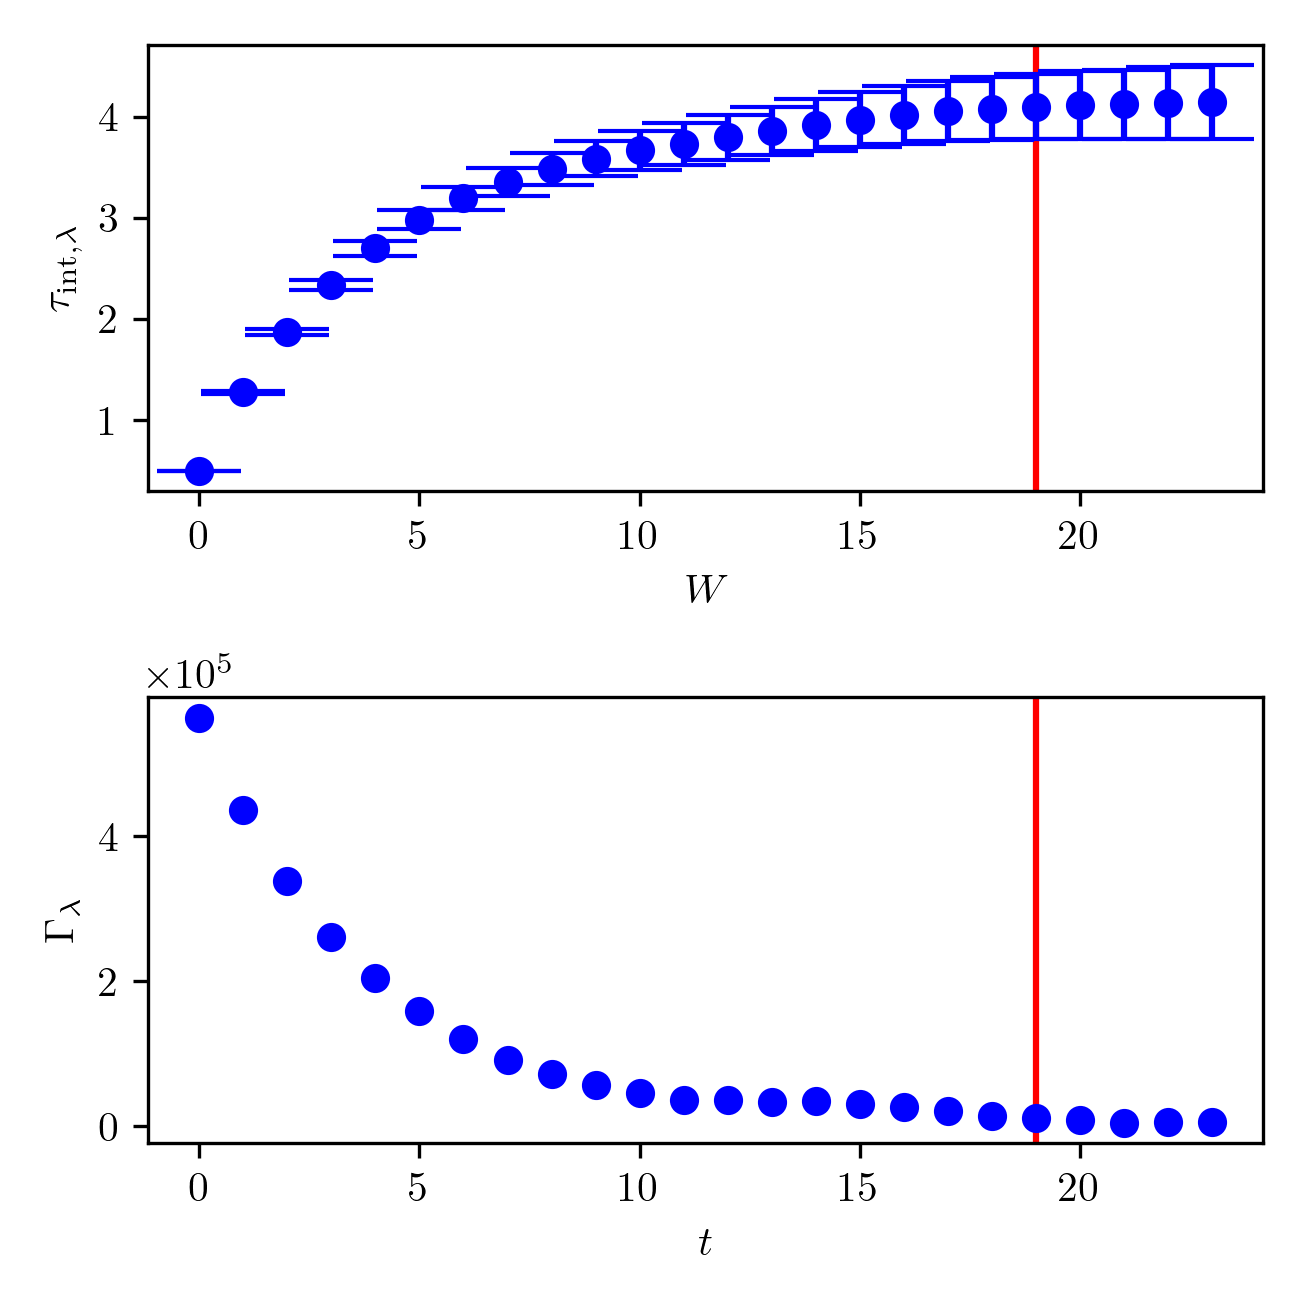
\includegraphics{UwerrTauIntFirstO3lam.png}
	\caption[IACT of $\lambda \sim \pi( \cdot| \bm{y})$, for linear model.]{Provided by \cite{drikHesse}, the IACT $\tau_{\text{int},\lambda}$ at summation windows W as well as the estimated autocorrelation function $\Gamma_{\lambda}$ at lag $t$ of the samples $\lambda \sim \pi( \cdot| \bm{y})$.}
	\label{fig:IATCLamLin}
\end{figure}


\subsubsection{TT approximation of marginal posterior}
Alternatively, the square root of the marginal posterior over a predefined grid can be approximated by a TT to calculate the marginals $\pi(\gamma|\bm{y})$ and $\pi(\lambda|\bm{y})$ (see Sec.~\ref{subsec:TTMarg}).

The univariate grid is defined over $\gamma = [ 0.8 \times 10^{15},1.2 \times 10^{16}]$ and $\lambda = [ 10^{-5}, 8 \times 10^{-4}]$ with $n = 20$ grid points (see Fig.~\ref{fig:MeanVarError}, where we argue for the number of grid points).
The ``normalisation constant'' is set to $c=-150$ so that the values of $\sqrt{\pi( \lambda,\gamma| \bm{y})} = \exp \{ 0.5 \log  \pi(\lambda,\gamma | \bm{y}) + c \} $ are within computer precision.
 %-320/2
Then we initialise \linebreak the~\texttt{tt.cross.rectcross.rect\_cross.cross} function based on the TT cross algorithm in~\cite{OSELEDETS2010TTCross,Dolgov2018TTCross} from the Python package \texttt{ttpy}~\cite{Oseledets2018ttpy} with a random tensor.
The number of ranks $r = 4$ is constant and we do one sweep with $2n_{\text{sweeps}}2nr =400$ function evaluations and obtain a TT approximation of $\pi( \lambda,\gamma| \bm{y})$ in about $0.02$s.
Ironically, this the same number of functions evaluations to approximate a $20 \times 20$ point grid.
The TT format is especially advantageous for larger grid sizes and higher dimensional parameter spaces.
To compute the marginals $\pi(\lambda| \bm{y})$ and $\pi(\gamma| \bm{y})$ the TT error is set to $\xi = 1 / \uplambda (\mathcal{X})$ because we observe peak values of around $10^{47}$.
For Cartesian basis the Mass matrix becomes $\bm{M}_k = \text{diag}(\uplambda_k(\mathcal{X}_k))$ (see Eq.~\ref{eq:MassMat}) with and $\uplambda(x) = 1$ .
The coefficient tensor $\bm{B}$ and $\bm{R}_{\text{pre}}$ are calculated as in Prop.~\ref{prob:backMarg} and Prop.~\ref{prob:ForMarg} (see Sec.~\ref{subsec:TTMarg}).

We plot the TT approximation as a colour map on top of the obtained samples in Fig.~\ref{fig:ScatterPlotTT}.
The relative RMS TT approximation error over the whole grid is $\approx 7\%$ and similar to the propagation error in $\pi(\lambda, \gamma| \bm{y})$ due to the approximations of $f(\lambda)$ and $g(\lambda)$ (see further up).
\begin{figure}[h!]
	\centering
	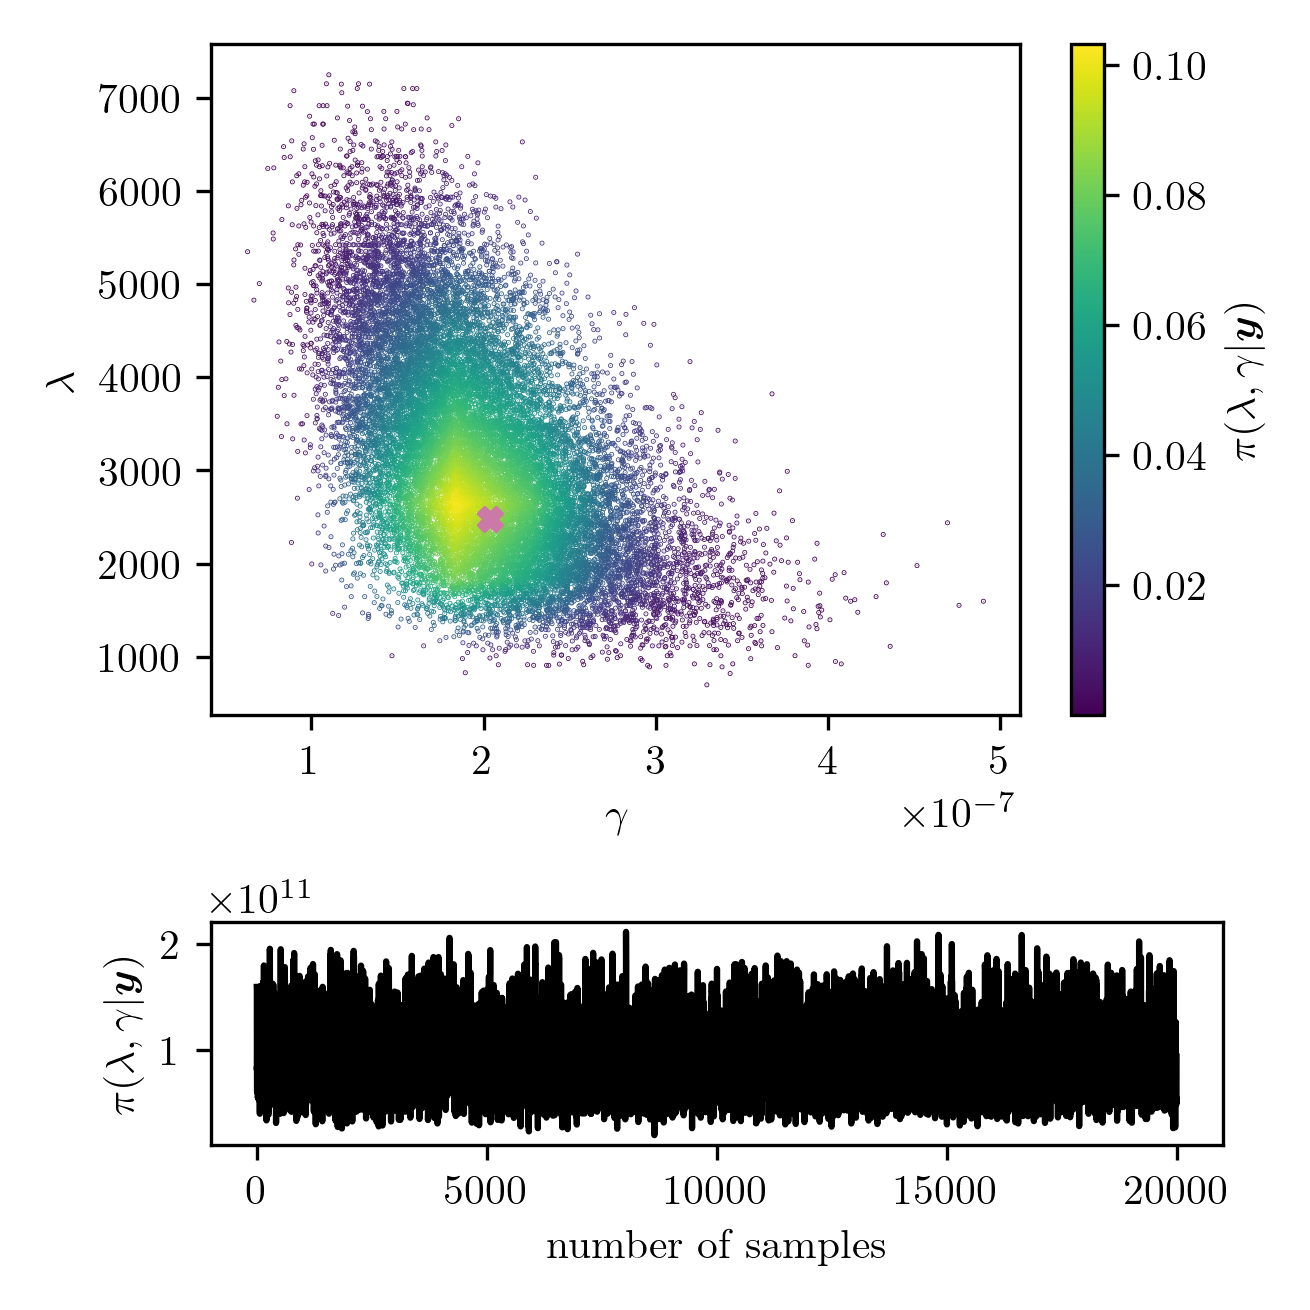
\includegraphics{ScatterplusHistoPlusTT.png}
	\caption[Samples from marginal posterior and TT approximation; trace plot of the MWG for $\pi(\lambda, \gamma| \bm{y})$]{Samples from the marginal posterior colour-coded using the TT approximation of $\pi(\lambda , \gamma  | \bm{y})$. The mode of $(\lambda_0 , \gamma_0)$ of $\pi(\lambda , \gamma  | \bm{y})$ is marked with the pink cross. To show ergodicity, we plot the trace of the samples of the MWG algorithm.}
	\label{fig:ScatterPlotTT}
\end{figure}
%\subsubsection{Sample from Marginal Posterior Distribution}
%\label{subsec:firstMarg}

%\begin{algorithm}[!ht]
%	\caption{Metropolis within Gibbs for $\pi(\lambda, \gamma | \bm{y})$}
%	\begin{algorithmic}[1]
	%		\STATE Initialise  \( \bm{\theta}^{(0)}  =( \lambda^{(0)} , \gamma^{(0)}  ) \) and set burn-in $N_{\text{burn-in}}$
	%		\FOR{ \( k = 1, \dots, N^{\prime} \)}
	%		\STATE Propose \( \lambda \sim \mathcal{N}(\lambda^{(t-1)}, 0.8 \lambda_0)  \)
	%		\STATE Compute
	%		\[ \alpha( \lambda  | \lambda^{(t-1)}) = \min \left\{ 1, \frac{\pi(\lambda | \gamma^{(t-1)}, \bm{y})  }{\pi(\lambda^{(t-1)}| \gamma^{(t-1)}, \bm{y})}  \right\} \]
	%		\STATE Draw $u \sim \mathcal{U}(0,1)$
	%		\IF{$\alpha \geq u$ }
	%		\STATE Accept and set \( \lambda^{(t)} = \lambda \)
	%		\ELSE  
	%		\STATE Reject and keep \(\lambda^{(t)} = \lambda^{(t-1)} \)
	%		\ENDIF
	%		\STATE Draw $\gamma^{(t)} | \lambda^{(t)} ,\bm{y} \sim \text{Gamma} \big( 0.5  \, m + 2, 0.5 \, f(\lambda^{(t)}) + 10^{-10}(1 + \lambda^{(t)}) \big) $
	%		\ENDFOR
	%		%\STATE Output: $ \bm{\theta}^{(N_{\text{burn-in}})}, \dots,  \bm{\theta}^{(k)} , \dots,   \bm{\theta}^{(N)} \sim \pi(\bm{\theta}| \bm{y}) $
	%		\STATE Output: $ (\lambda, \gamma)^{(N_{\text{burn-in}})}, \dots,  (\lambda, \gamma)^{(k)} , \dots,   (\lambda, \gamma)^{(N)} \sim \pi(\lambda, \gamma| \bm{y}) $
	%	\end{algorithmic}
%	\label{alg:margPost}
%\end{algorithm}



%
%We find the mode at the minimum of  $-\log\{ \pi(\lambda, \gamma | \bm{y}) \}$  using \texttt{scipy.optimize.fmin} function and limit the number of function evaluation to 25 and use Cholesky back and forward substitution to calculate values of $g(\lambda)$ and $f(\lambda)$.
%Additionally, we calculate $\bm{B}_0^{-1} \bm{L} $ and  $\bm{B}_0^{-1}  \bm{A}_L^T \bm{y}$ once more at $\lambda_0$ and plot the Taylor approximation within the sampling region in Fig. \ref{fig:fandg}.
%\subsection{Posterior distributions with Linear model for Ozone -- MTC}
%\label{sec:firstMTC}
%In this section we calculate the posterior marginal and then conditional (MTC) posterior distribution for ozone conditioned on the ground truth temperature and pressure profiles using the linear forward model $\bm{A}_L$.
%This is faster then the other way round (finding temperature over pressure conditioning on ozone) and temperature and pressure are well defined within the atmosphere so it is easier to just condition on a temperature and pressure profile out of a text book.
%We employ a so-called Metropolis within Gibbs (MWG) algorithm on the marginal posterior as summarised in the algorithmic Box \ref{alg:margPost} or use a Tensor-Train (TT) approximation to calculate marginal posterior values.
%Then we can either sample from the conditional posterior using the randomise then optimise (RTO) method or calculate conditional mean and variance using quadrature.
%The DAG in Fig. \ref{fig:DAGO3} visualises that process and we can show explicitly that we group the hyper-parameters $\delta, \gamma$ together to determine the marginal posterior $\pi(\gamma, \delta | \bm{y})$.
%Here $\gamma$ , the noise parameter, determines the noise precision $\bm{\Sigma} = \gamma ^{-1} \bm{I}$ and $\delta$, the smoothness parameter, the precision matrix $\bm{Q} = \delta \bm{L}$ of the prior distribution for $\bm{x}$.
%Then conditioned on the hyper-parameters the conditional posterior $\pi( \bm{x} |\gamma, \delta, \bm{y})$ gives the distribution of posterior ozone profiles.
%Note that we use the linear model $A_L$ here as we do not have an approximation to the non-linear model yet and all prior distributions are defined in Table \ref{tab:priors}.
%The full posterior $\pi(\bm{x},\gamma, \delta | \bm{y}) =  \pi(\bm{x}|\gamma, \delta ,\bm{y}) \pi(\gamma, \delta | \bm{y}) $ is given by multiplication of the marginal and conditional posterior densities. 
%\begin{align}
%	\bm{x} |  \bm{\theta}, \bm{y} \sim \mathcal{N} \Big(
%	\underbrace{\bm{\mu} + \left( \bm{A}^T \bm{\Sigma}^{-1} \bm{A} + \bm{Q} \right)^{-1} \bm{A}^T \bm{\Sigma}^{-1} (\bm{y} - \bm{A} \bm{\mu})}_{\bm{\mu}_{\bm{x} |  \bm{\theta}, \bm{y}}},
%	\underbrace{ \left( \bm{A}^T \bm{\Sigma}^{-1} \bm{A} + \bm{Q} \right)^{-1} }_{\bm{\Sigma}_{\bm{x} |  \bm{y}, \bm{\theta}}}
%	\Big) \, ,
%\end{align}
%is normal distribution and we compute weighted expectations, as in Eq.~\ref{eq:MargExpPos}, of the conditional mean and covariance matrix, where the weights are given by $\pi(\bm{\theta} | \bm{y})$. 
%Note that both the noise covariance $\bm{\Sigma} = \bm{\Sigma}(\bm{\theta})$ and the prior precision matrix $\bm{Q} = \bm{Q}(\bm{\theta})$ depend on the hyper-parameters $\bm{\theta}$.
\subsection{Full Conditional Posterior}
\label{subsec:firstCond}

Finally, we can evaluate the normally distributed full conditional posterior distribution
\begin{align}
	\bm{x}| \delta, \gamma, \bm{y}  \sim \mathcal{N}\big( \underbrace{ (\bm{A}^T \bm{A} + \delta / \gamma \bm{L} )^{-1} \bm{A}^T \bm{y}}_{\bm{x}_{\lambda}}, ( \underbrace{ \gamma \bm{A}^T \bm{A} + \delta \bm{L} }_{\gamma \bm{B}_{\lambda}}  )^{-1} \big) \, \label{eq:CondPost},
\end{align}
as in Eq. \ref{eq:CondPostLin}, with $\lambda = \delta / \gamma $.
\begin{figure}[ht!]
	\centering
	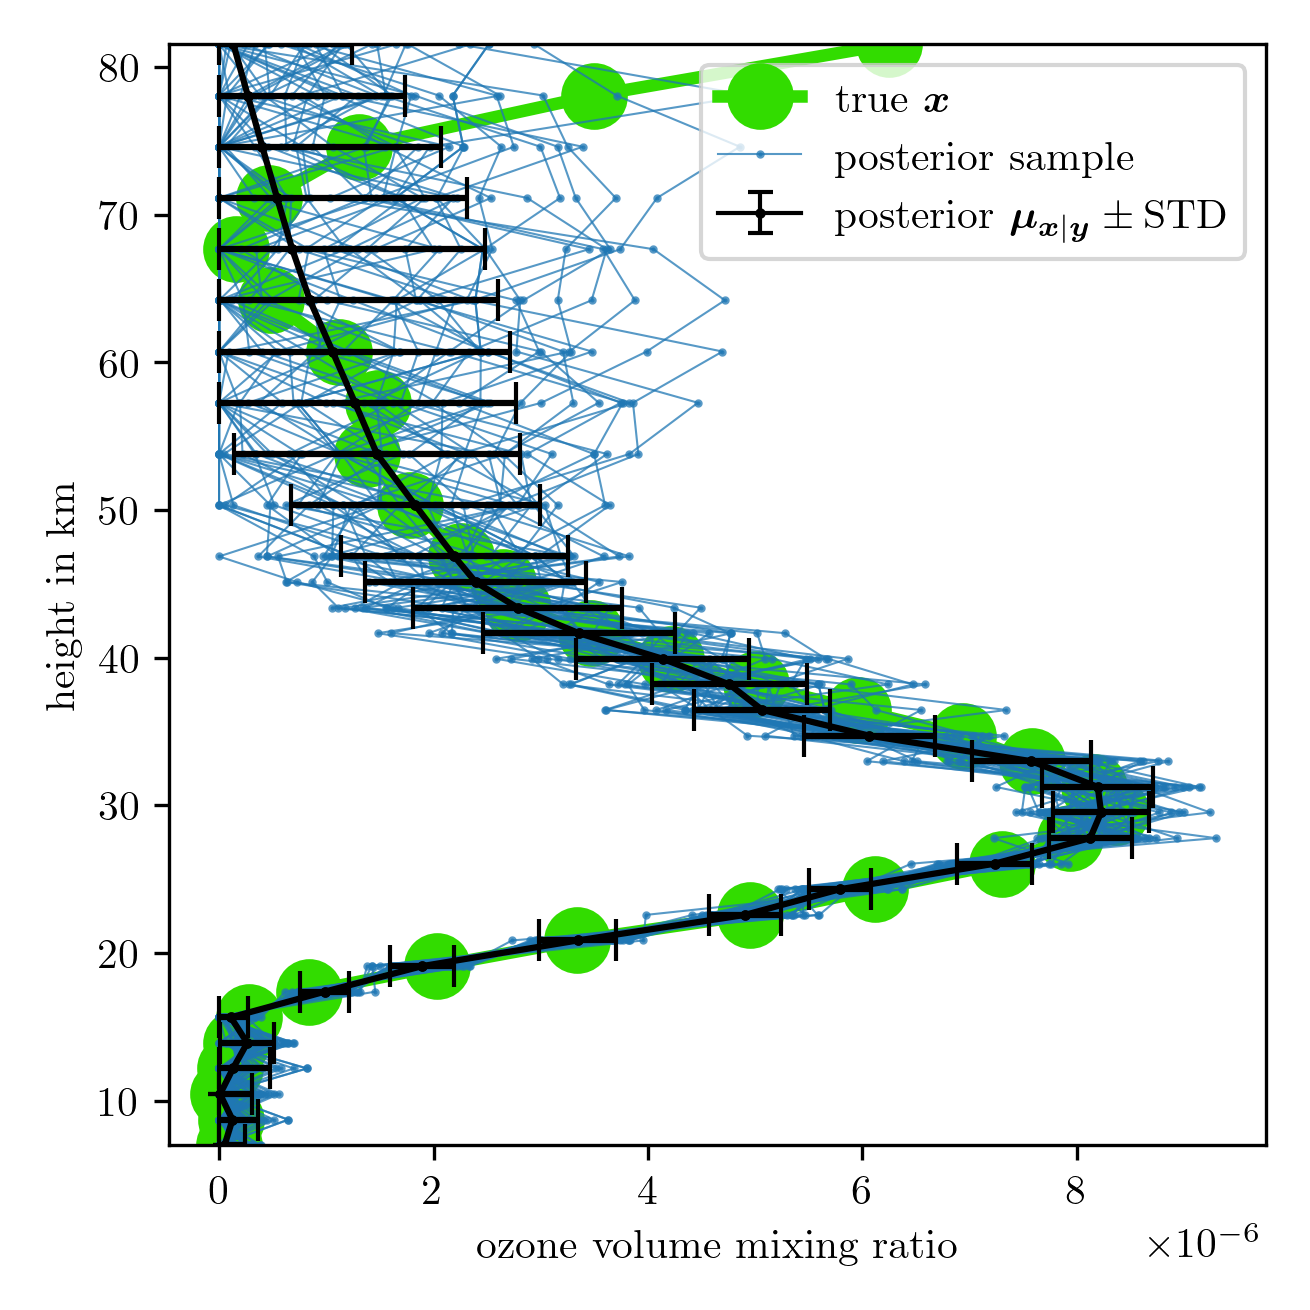
\includegraphics{FirstTestRes.png}
	\caption[Ozone samples of the full posterior.]{Ozone samples from the full posterior distribution $\pi(\bm{x}| \bm{y})$ after characterising posterior mean and covariance by weighted expectations over the marginal posterior $\pi(\lambda,\gamma | \bm{y})$ based on the linear forward map $\bm{A}_L$. We set negative ozone VMR values to zero.}
	\label{fig:O3Samp}
\end{figure}
In this thesis, we compute the posterior mean
\begin{align}
	\mu_{\bm{x}|\bm{y}} = \int \bm{x}_{\lambda} \pi(\lambda| \bm{y}) \diff\lambda \approx \sum \bm{x}_{\lambda_i} \pi(\lambda_i| \bm{y}) \, , \label{eq:MeanInt}
\end{align} and posterior covariance
\begin{align}
	\Sigma_{\bm{x}|\bm{y}} = \int \gamma^{-1}  \pi(\gamma | \bm{y} ) \, \diff \gamma \, \int  \bm{B}_{\lambda}^{-1} \, \pi(\lambda | \bm{y} )  \, \text{d} \lambda  \approx \sum {\gamma_i}^{-1}\pi(\gamma_i| \bm{y}) \sum \bm{B}_{\lambda_i}^{-1}\pi(\lambda_i| \bm{y})\, \label{eq:CovInt}
\end{align}
of $\pi(\bm{x}| \bm{y})$ as weighted expectations over the marginal posterior $\pi(\lambda,\gamma | \bm{y})$ by quadrature \cite[Sec. 2.1]{Dick_Kuo_Sloan_2013} with $\sum \pi(\lambda_i| \bm{y}) = \sum \pi(\gamma_i| \bm{y}) = 1$.
The weights $\pi(\lambda_i| \bm{y})$ and $\pi(\gamma_i| \bm{y})$ are either given by the TT approximation or by the bars of the sample-based histograms.
More precisely, the heights of the sample-based histogram bars act as quadrature weights, where $\lambda_i$ is defined at the centre of each bar.
We use the Cholesky decomposition of $\bm{B}_{\lambda} = \bm{A}^T \bm{A} + \lambda \bm{L}$ to invert $\bm{B}_{\lambda}$ and to calculate $\bm{x}_{\lambda} = (\bm{A}^T \bm{A} + \lambda \bm{L} )^{-1} \bm{A}^T \bm{y}$ both via \texttt{scipy.linalg.cho\_solve}.
It is sufficient to evaluate $\bm{x}_{\lambda}$ and invert $\bm{B}_{\lambda}$ 20 times to obtain mean and covariance values of $\pi(\bm{x}|\bm{y})$ within a reasonable error (see Fig.~\ref{fig:MeanVarError}).
Finding the mode of $\pi(\lambda,\gamma|\bm{y})$, running the TT \texttt{cross}, calculating the marginals and the posterior mean and covariance takes $0.025$s.
The MWG sampler takes $\approx0.5$s for the same results, so most computational effort lays within the sampling procedure and the time to calculate posterior mean and covariance is negligible.
The posterior samples of $\pi(\bm{x}|\bm{y})$ are plotted in Fig.~\ref{fig:O3Samp} with negative ozone values set to zero.
The fact that we have to deal with negative ozone values is due to the poor prior choice in $\pi(\bm{x}|\delta)$.
%Note that the sample mean is slightly larger than the posterior mean at heights where the data is noise-dominated, and the ozone values are determined by the prior, or where the ground truth is close to zero.
This indicates that one should use a different, more physically based prior or a better model for ozone in the atmosphere.
Note that the posterior samples do not capture the second ozone peak at around $80$km.

If calculating the variance is too costly, see Sec.~\ref{subsec:RTO} where we present a feasible alternative to draw a sample from the full conditional posterior.


%\subsubsection{Randomize then optimize -- RTO}
%For the RTO method we start by drawing an independent hyper-parameter sample $ ( \delta, \gamma) \sim \pi(\delta, \gamma | \bm{y})$ from the samples of the MwG.
%Then we generate two independent Gaussian random variables $\bm{v}_1 \sim \mathcal{N}(\bm{0},\gamma  \bm{A}^T_L \bm{A}_L)$ and $\bm{v}_2 \sim \mathcal{N}(\bm{0}, \delta \bm{L})$.
%Here  can use Cholesky factorisation of $\bm{L} =\bm{L}_C\bm{L}^T_C $ and the multiplication rule for normal distributions so that $\bm{v}_1 \sim \sqrt{\gamma} \bm{A}_L^T \mathcal{N}(0,\bm{I})$ and $\bm{v}_2 \sim \sqrt{\delta} \bm{L}_C \mathcal{N}(0,\bm{I})$.
%Then we solve
%\begin{align}
%	\label{eq:FirstRTO}
%	\left( \gamma \bm{A}_L^T  \bm{A}_L +\delta \bm{L} \right) \bm{x} = \gamma \bm{A}_L^T \bm{y} + \bm{v}_1 + \bm{v}_2 \, ,
%\end{align}
%using Cholesky back and forward substitution, for $\bm{x}$ and obtain one independent sample of $\pi(\bm{x}|\bm{y}, \bm{\theta})$.
%See Fig. \ref{fig:O3Samp}, where we plot $m = $ samples of the conditional posterior.
%
%The histogram in is binned as we intergate over it to 7 bins





\subsubsection{Eigenvalues full conditional posterior covariance}
\begin{figure}[ht!]
	\centering
	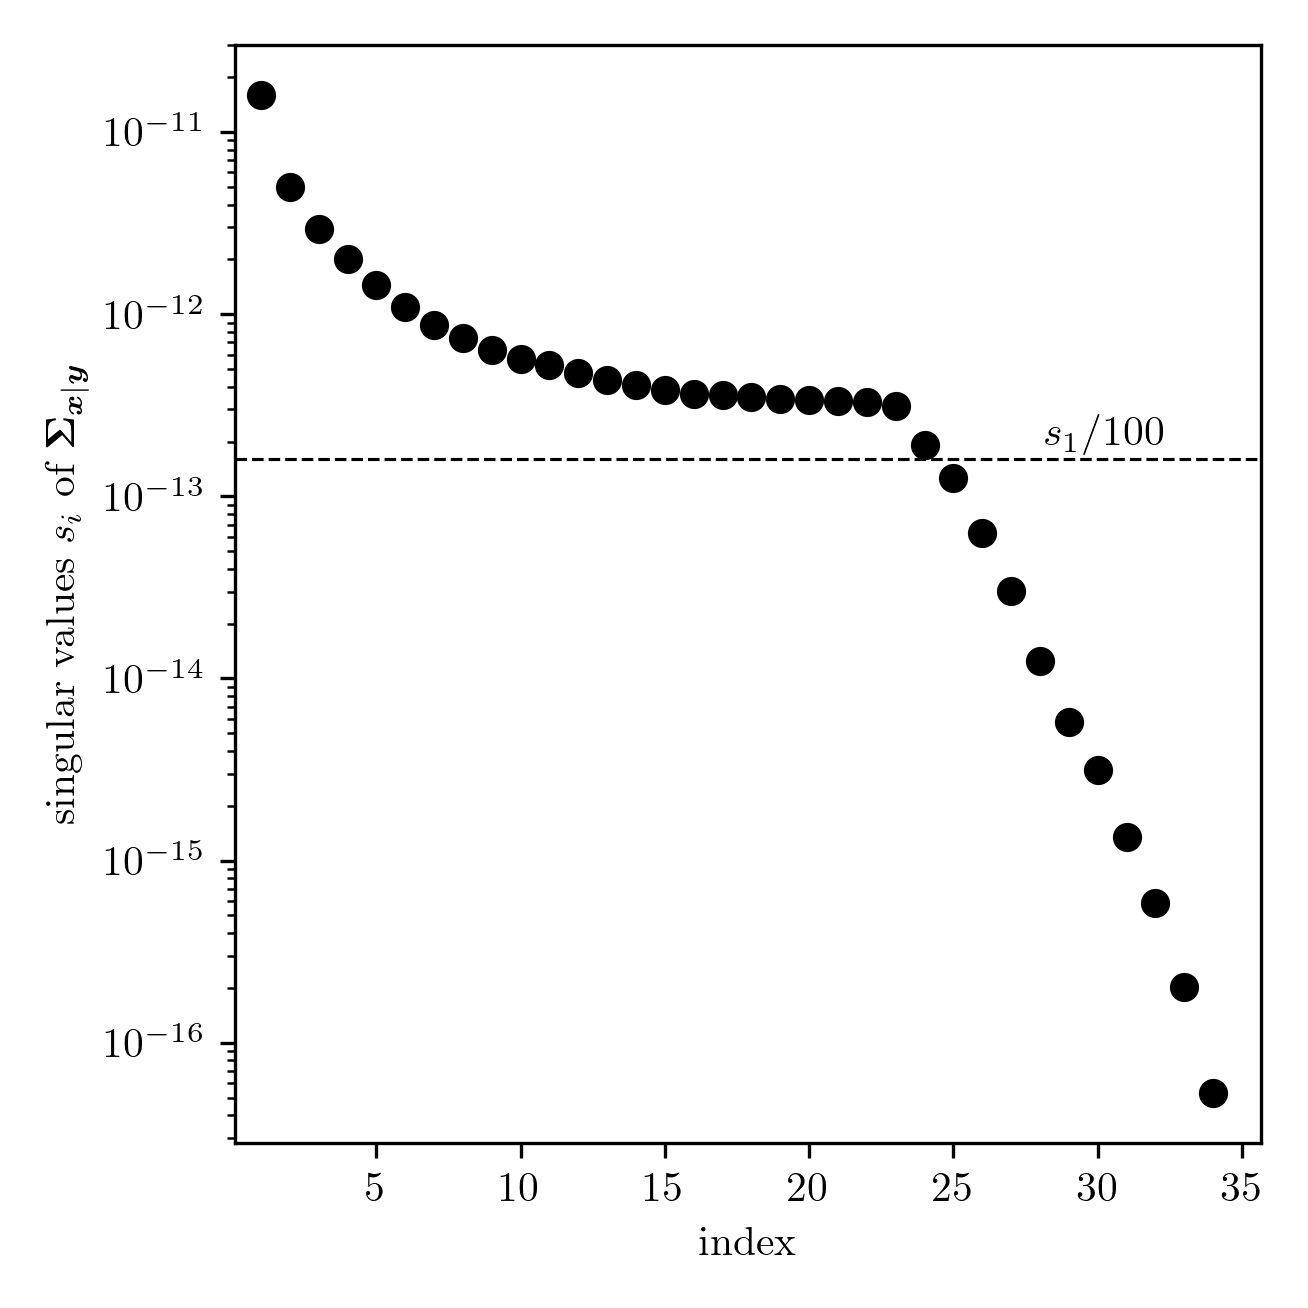
\includegraphics{CovSing.png}
	\caption[Eigenvalues of the posterior precision matrix]{Eigenvalues of the precision matrix of $\bm{Q}_{ \bm{x}|\delta, \gamma, \bm{y}}= \gamma \bm{A}^T \bm{A} + \delta \bm{L}$ of the full conditional posterior distribution $\pi(\bm{x}|\delta, \gamma, \bm{y})$ for ozone.
		We see that large eigenvalues of $\bm{Q}_{ \bm{x}|\delta, \gamma, \bm{y}} $ are unaffected by the prior.
		For small eigenvalues of $\gamma \bm{A}^T \bm{A}$ the eigenvalues of $\bm{Q}_{ \bm{x}|\delta, \gamma, \bm{y}} $ are dominated by the structure of the eigenvalues of $ \delta \bm{L}$.}
	\label{fig:PostCov}
\end{figure}
In Fig.~\ref{fig:PostCov} the eigenvalues (ordered in size) of the precision matrix $\bm{Q}_{ \bm{x}|\delta, \gamma,\bm{y}}=  \gamma \bm{A}^T \bm{A} + \delta \bm{L} $ for a random $\delta,\gamma \sim \pi(\delta,\gamma|\bm{y})$ are plotted and compared to the eigenvalues of the prior precision matrix $\delta \bm{L}$ and $\gamma \bm{A}^T \bm{A}$.
We observe that the larger eigenvalues of $\bm{Q}_{ \bm{x}|\delta, \gamma,\bm{y}}$ are very much the same as the larger eigenvalues of $\gamma \bm{A}^T \bm{A}$.
Once the eigenvalues of $\gamma \bm{A}^T \bm{A}$ are significantly smaller than the eigenvalues of $\bm{Q}_{ \bm{x}|\delta, \gamma,\bm{y}}$ the structure of the eigenvalues is dominated by the eigenvalues of $\delta \bm{L}$.
The eigenvectors corresponding to the 12 largest eigenvalues of $\bm{Q}_{ \bm{x}|\delta, \gamma,\bm{y}}$ include ozone profile structure at lower altitudes up to $35$km, where the other eigenvectors mainly represent structures above $30$km (see Fig.~\ref{fig:CovEigVec1} and Fig.~\ref{fig:CovEigVec2}).
Note that the eigenvalues of each matrix may correspond to different eigenvectors, even if the eigenvalues are the same.

\subsubsection{Errors of Full Posterior Mean and Covariance}
\begin{figure}[ht!]
	\centering
	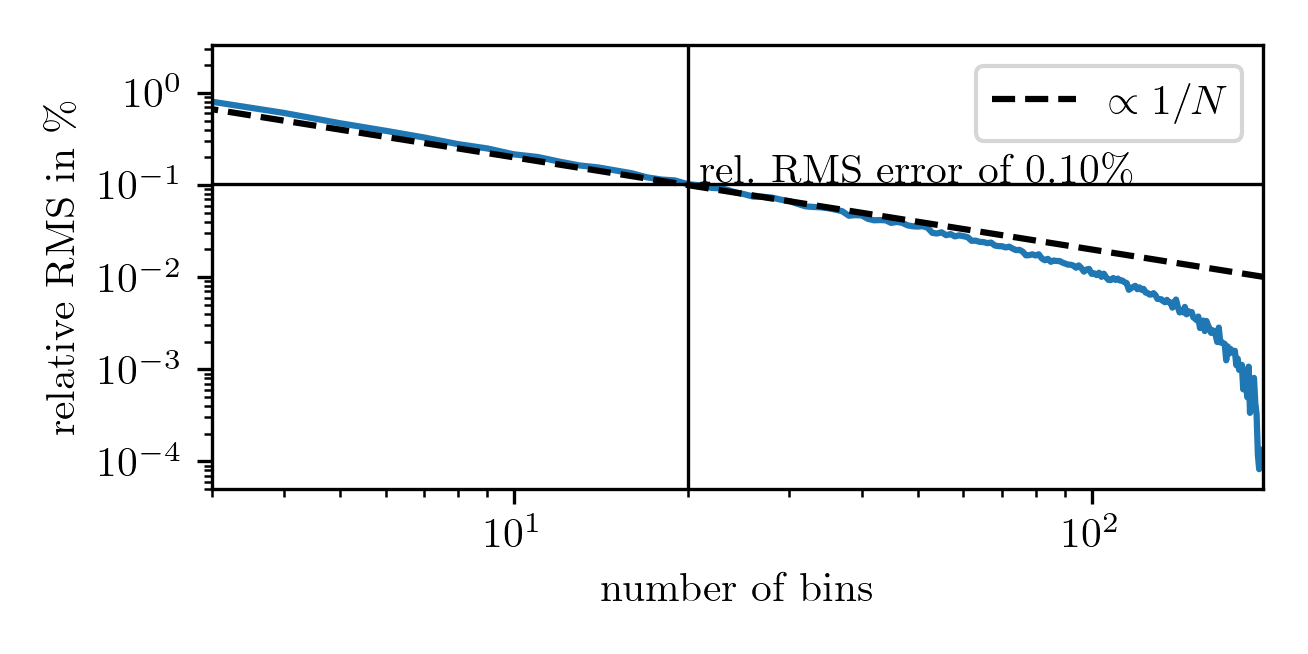
\includegraphics{relErrO3MeanVar.png}
	\caption[Relative Error of full posterior mean and covariance.]{Relative RMS error of $\bm{\mu}_{\bm{x}|\bm{y}}$ and covariance $\bm{\Sigma}_{\bm{x}|\bm{y}}$ calculated by the weighted expectations and compared to a ``ground truth'' given by weighted expectations over 200 bins.}
	\label{fig:MeanVarError}
\end{figure}
In Fig. \ref{fig:MeanVarError}, we plot the relative RMS error for the mean $\bm{\mu}_{\bm{x}|\bm{y}}$ and covariance $\bm{\Sigma}_{\bm{x}|\bm{y}}$ of $\pi(\bm{x}|\bm{y})$ due to grid size or number of bins of the marginal posterior.
Those results are obtained by calculating the weighted expectation over normalised histograms of $\pi(\lambda,\gamma | \bm{y})$, where the number of bins is increased and compared to a solution calculated from a histogram with 200 bins.
The relative error behaves roughly proportional to $1/N$, and we consider a relative RMS error less than $0.5\%$ good enough, which is easily met at 20 bins.
This sets the TT grid size and the number of evaluations of $\bm{x}_{\lambda}$ (posterior mean, see Eq.~\ref{eq:MeanInt}) and $(\gamma \bm{B}_{\lambda})^{-1}$ (posterior covariance, see Eq.~\ref{eq:CovInt}).

%marginal Ozone Pressure Temperature
%\clearpage


\section{Solution by Regularisation}
\label{sec:SolByReg}
Since we claim that the a hierarchical Bayesian framework provides more information than regularisation methods, we compare the MTC scheme to a regularisation approach.
That is why the chosen linear-Gaussian Bayesian framework is most similar to the here used regularisation approach~\cite{fox2016fast}.

The regularised solution is defined as in~\cite{hansen2010discrete, fox2016fast} 
\begin{align}
	\bm{x}_{\lambda} =\underset{ \bm{x}}{\arg \min}\,  \lVert \bm{A}\bm{x} - \bm{y} \rVert_{L^2}^2 + \lambda \bm{x}^T \bm{L} \bm{x} \, ,
	\label{eq:XLam}
\end{align}
with the regularisation parameter $\lambda$, linear forward model matrix $\bm{A}$ and data $\bm{y}$.
A regularised solution
\begin{align}
	\bm{x}_{\lambda} = (\bm{A}^T\bm{A} + \lambda \bm{L} )^{-1} \bm{A}^T \bm{y} \label{eq:xLam} \, 
\end{align}
is calculated as in Sec.~\ref{sec:reg}.


The regularised solution is found using the L-curve method following~\cite{hansen1993use}.
Within this method we compute $\bm{x}_\lambda$, for 200 different $\lambda$ values in between $10^{-8}$ to $10^{0}$ and plot the regularisation norm $\sqrt{\bm{x}_\lambda^T\mathbf{L} \bm{x}_\lambda}$ against the data misfit norm $\lVert \bm{A}\bm{x}_\lambda - \bm{y} \rVert_{L^2}$ (see Figure \ref{fig:LCurve}). 
The regularised solution corresponds to the ``corner'' of the L-curve at the point of maximum curvature provided by the kneedle algorithm~\cite{satopaa2011kneedle} using the function \texttt{kneed.KneeLocator} in $\approx 0.015$s, which is slightly faster then the TT approach to obtain posterior mean and covariance.
The corresponding regularisation parameter is $\lambda = 1.6 \times 10^{-4}$.

\begin{figure}[ht!]
	\centering
	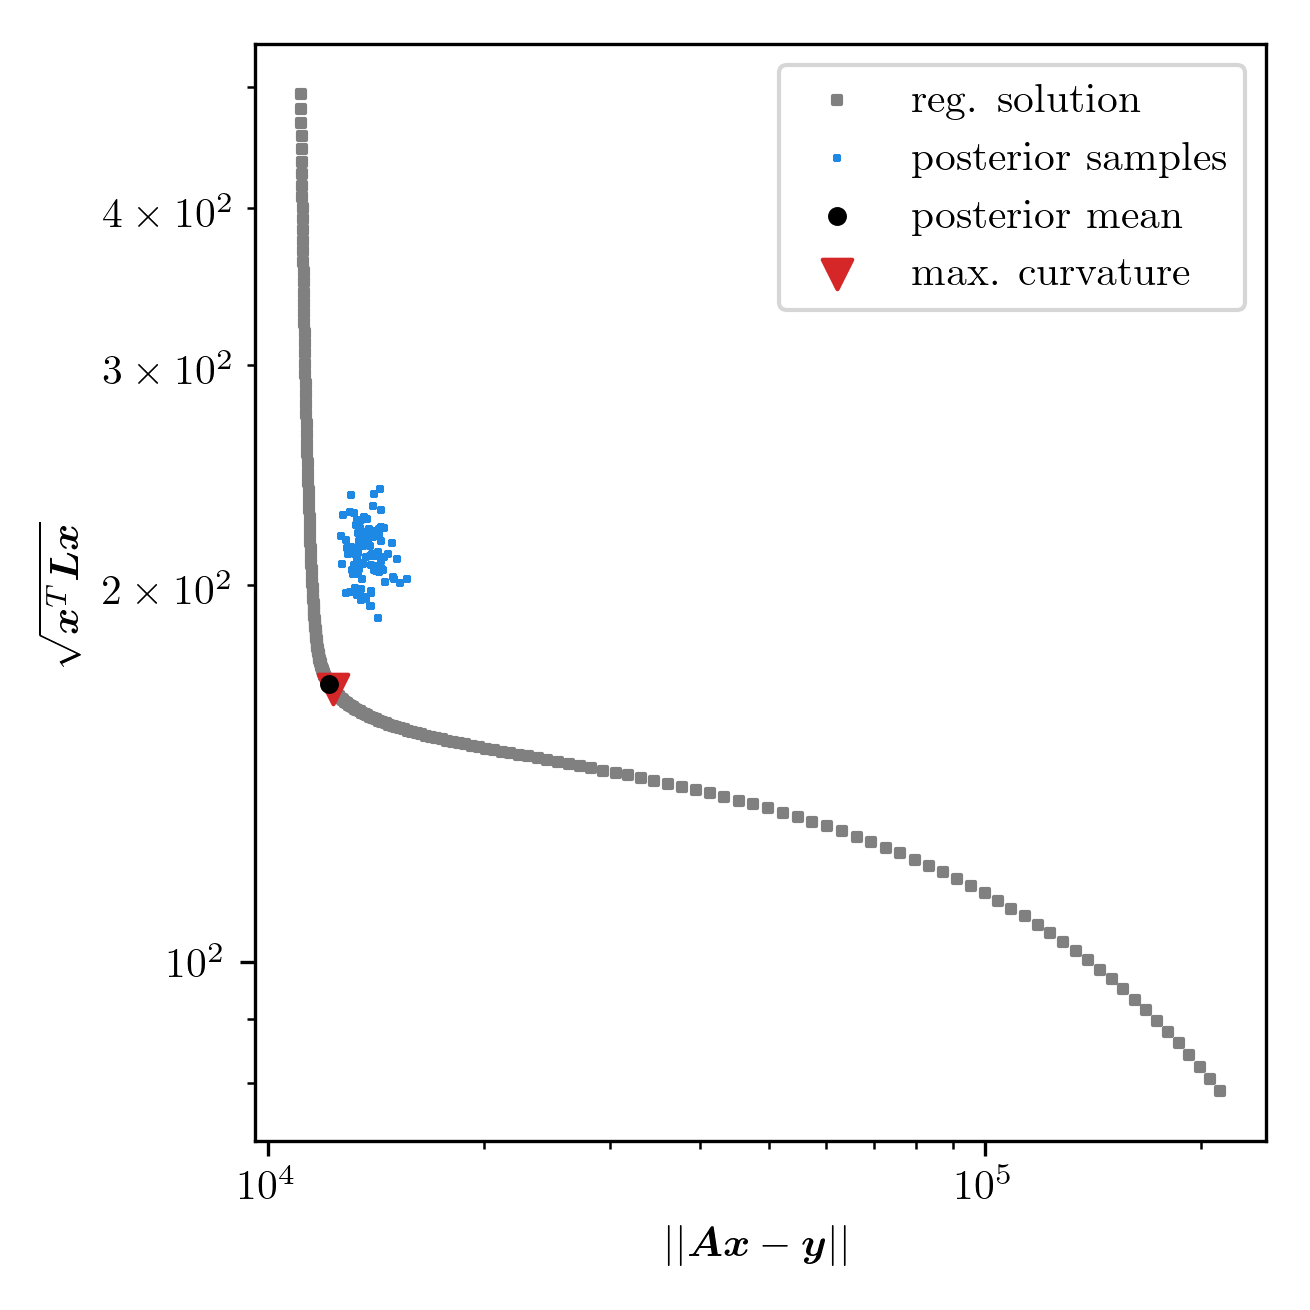
\includegraphics{LCurvePhD.png}
	\caption[Plot of the L-curve to find the regularised solution.]{L-curve of regularisation norm $\sqrt{\bm{x}^T\bm{Lx}}$ against the data misfit norm $\lVert \bm{A}\bm{x} - \bm{y} \rVert_{L^2}$ for different $\lambda$ values, where $\bm{x}_{\lambda}$ is calculated as in Eq.~\ref{eq:xLam}. The best regularised solution is located at the point of maximum curvature (pink triangle) of the L-curve. Additionally, we calculate the data misfit norm and the regularised norm for the mean (black circle) and samples (blue squares) of the full posterior of ozone.}
	\label{fig:LCurve}
\end{figure}
The regularised solution in Fig.~\ref{fig:O3SolplsReg} is very similar to the posterior mean and both have a similar data misfit and regularisation norm.
Neither the regularisation solution nor the posterior ozone profiles capture the second ozone peak of the ground truth at high altitudes.
Note that we cannot infer the posterior mean from the regularised solutions, even if it appears to lie on the L-curve.
It is pretty clear that the regularised solution accounts for only one possible solution and does not provide uncertainties. The regularised solution and the posterior mean are not similar to the samples drawn from the posterior $\pi(\bm{x}| \bm{y})$ (see Fig.~\ref{fig:O3Samp}).
All posterior samples of $\pi(\bm{x}| \bm{y})$ are less regularised and lie above the L-curve, and as already mentioned, are all feasible solutions to the data.
This does make sense, if one thinks about the mean as the (smooth) average over less-smooth samples and the regularised solution as an extremely smooth ozone profile (see Lagrangian in Sec.~\ref{sec:reg}).

Counterintuitively it is not possible to obtain a sample that represents the mean of a multivariate probability distribution~\cite[Sec.~3.1]{VershyninMultiD2018}.
%, despite it being the point of the highest probability.
This is because the probability mass in a mutli-dimensional space concentrates on a “shell” or “ring” away from the mean~\cite{VowelsMultiD}.
Alternatively, think about how an electron's mean position may be inside the atom's core but the electron can never be observed at the centre of the atom's nucleus~\cite[Fig.~4]{ElectronBessel}.




\chapter{Affine Approximation of the Non-Linear Model}
\label{ch:affine}
\thispagestyle{empty}
\newcommand*{\vertbar}{\rule[-1ex]{0.5pt}{2.5ex}}
\newcommand*{\horzbar}{\rule[.5ex]{2.5ex}{0.5pt}}
The forward map, introduced in Chapter~\ref{ch:formodel}, poses a weakly non-linear forward problem.
One could tackle the non-linearity by treating the inverse problem as a linear inverse problem and then iteratively updating the non-linear part after each parameter sample.
Instead, as in Fig.~\ref{fig:affinStrat} illustrated, we approximate the non-linear model using an affine map, which is a linear map with a translation, e.g. $\bm{A}\bm{x} + \bm{b}$, and maps Gaussians onto Gaussians.
Here we find an affine map $\bm{M}$ based on the linear model $\bm{A}_L$ that provides an approximation of the non-linear model $\bm{A}(\bm{x})$ for parameters $\bm{x}$ near the posterior mean $\bm{\mu}_{\bm{x}|\bm{y}}$.
\begin{figure}[htb!]
	\centering
	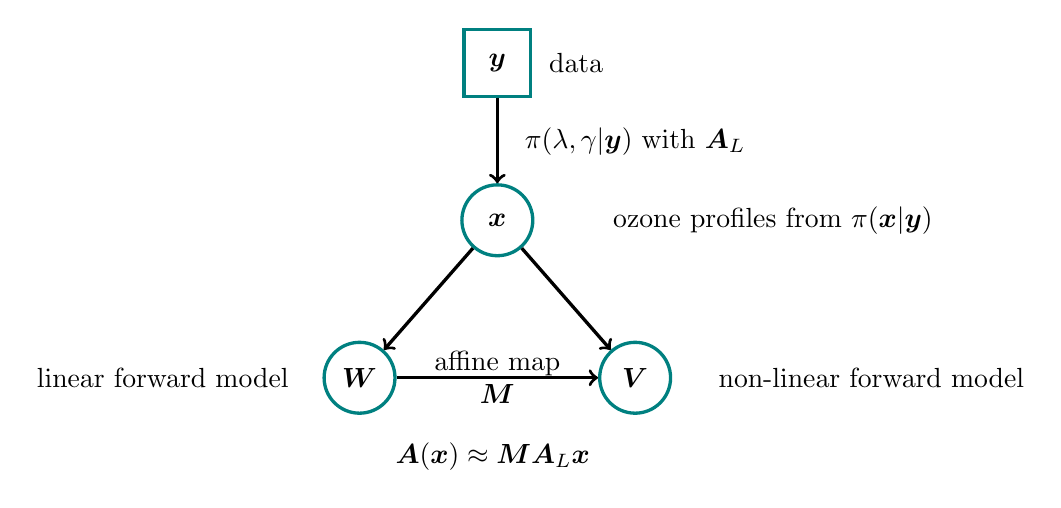
\begin{tikzpicture}
		\node[rectnode] at (0,0) (Oy)    {$\bm{y}$};
		\node[roundnode2] at (0,-2) (x)     {$\bm{x}$};
		\node[roundnode2] at (1.75,-4) (V)    {$\bm{V}$};%{$\bm{A}_{NL}\bm{x}$};
		\node[roundnode2] at (-1.75,-4) (W)    {$\bm{W}$};%{$\bm{A}_L\bm{x}$};
		\draw[->, very thick] (Oy.south) -- (x.north); 
		\draw[->, very thick] (x) -- (V); 
		\draw[->, very thick] (x) -- (W); 
		\draw[->, very thick] (W.east) --  (V.west); 
		\node[align=center] at (1,0) (l1) {data};
		\node[align=center] at (3.5,-2) (f2) {ozone profiles from $\pi(\bm{x}|\bm{y}) $};
		\node[align=center] at (1.75,-1) (l1) {$\pi(\lambda , \gamma  | \bm{y})$ with $\bm{A}_L$};
		
		
		\node[align=center] at (-4.25,-4) (f3) {linear forward model};
		\node[align=center] at (4.75,-4) (f4) {non-linear forward model};
		\node[align=center] at (0,-5) (f5) {$\bm{A}(\bm{x}) \approx \bm{M A}_L \bm{x}$ };
		
		\node[align=center] at (0,-4) (f5) {affine map \\ $\bm{M}$};
		
	\end{tikzpicture}
	\caption[Strategy to find affine map.]{The strategy to find the affine map consists of first evaluating the marginal posterior for ozone $\pi(\lambda , \gamma  | \bm{y})$ based on the linear forward model. Based on ozone samples from the full posterior, we find an affine map $\bm{M}$ which approximates between noise-free linear data $\bm{A}_L$ and noise-free non-linear data $\bm{A}(\bm{x})$.}
	\label{fig:affinStrat}
\end{figure}

\section{Finding an Affine Map}

We find an affine map by creating the vector spaces $\bm{W}$ based on the linear forward model and $\bm{V}$ based on the non-linear forward model with ground truth pressure and temperature.
More specifically $m-1$ samples $\bm{x}^{(j)} \sim \pi(\bm{x}|\bm{y})$, for $j = 2, \dots,m$, from the posterior and the posterior mean $\bm{\mu}_{\bm{x}|\bm{y}}$ generate,
\begin{align*}
	\bm{W} = \begin{bmatrix}
		\vert& \vert&   &  \vert & & \vert \\
		\bm{A}_{L}  \bm{\mu}_{\bm{x}|\bm{y}} & \bm{A}_{L}  \bm{x}^{(2)}   &  \cdots& \bm{A}_{L} \bm{x}^{(j)} &  \cdots & \bm{A}_{L} \bm{x}^{(m)} \\
		\vert& \vert&   &  \vert & & \vert 
	\end{bmatrix}
	\in \mathbb{R}^{m \times m}
\end{align*}\noindent and
\begin{align*}
	\bm{V} = \begin{bmatrix}
		\vert& \vert&   &  \vert & & \vert \\
		\bm{A}(\bm{\mu}_{\bm{x}|\bm{y}} ) & \bm{A}(\bm{x}^{(2)}) &  \cdots& \bm{A}(\bm{x}^{(j)}) &  \cdots & \bm{A} (\bm{x}^{(m)})  \\
		\vert&\vert&   &  \vert & & \vert 
	\end{bmatrix} = 
	\begin{bmatrix}
		\begin{array}{ccc}
			\horzbar & v_{1} & \horzbar \\
			& \vdots    &          \\
			\horzbar & v_{j} & \horzbar \\
			& \vdots    &          \\
			\horzbar &v_{m} & \horzbar
		\end{array}
	\end{bmatrix}\in \mathbb{R}^{m \times m} \, .
\end{align*}
Then the non-linear forward model is approximated as 
\begin{align}
	\bm{A}(\bm{x}) \approx \bm{M A}_L \bm{x} \, , \label{eq:AffineM}
\end{align}
where we solve $v_j =r_j \bm{W}$ for each row $r_j$ in
\begin{align*}
	\bm{V}\bm{W}^{-1} = \bm{M} =
	\begin{bmatrix}
		\begin{array}{ccc}
			\horzbar & r_{1} & \horzbar \\
			& \vdots    &          \\
			\horzbar & r_{j} & \horzbar \\
			& \vdots    &          \\
			\horzbar &r_{m} & \horzbar
		\end{array}
	\end{bmatrix}\, \in \mathbb{R}^{m \times m} .
\end{align*}
using the Python function \texttt{numpy.linalg.solve}.
This is feasible since every noise-free measurement is independent of each other, and then every row $v_j$ of $\bm{V} \in \mathbb{R}^{m \times m}$ is independent of each other as well.
For an $\bm{x} = \bm{\mu}_{\bm{x}|\bm{y}} + \Delta \bm{x}$ we rewrite Eq.~\ref{eq:AffineM} to
\begin{align}
	\bm{A}(\bm{x})  \approx \underbrace{  \bm{M A}_L  \bm{\mu}_{\bm{x}|\bm{y}} }_{= \bm{A}( \bm{\mu}_{\bm{x}|\bm{y}} )  }+  \underbrace{\bm{M A}_L  \Delta \bm{x} }_{= \bm{A}^{\prime}( \bm{\mu}_{\bm{x}|\bm{y}} )  \Delta \bm{x} }\, \\
	=    \underbrace{ \bm{A}^{\prime}( \bm{\mu}_{\bm{x}|\bm{y}} ) \bm{x}}_{ \bm{A}\bm{x}}  +  \underbrace{ \bm{A}( \bm{\mu}_{\bm{x}|\bm{y}} )  - \bm{A}^{\prime}( \bm{\mu}_{\bm{x}|\bm{y}} ) \bm{\mu}_{\bm{x}|\bm{y}}}_{  \bm{b}}
\end{align}
to show that $ \bm{M}:\bm{A}_L\bm{x} \rightarrow \bm{A}(\bm{x})$ is an affine map.







%	\centering
%	\begin{tikzpicture}
%		\node[rectnode] at (2,-4) (NL)    {$\bm{V}$};
%		\node[rectnode] at (-2,-4) (L)    {$\bm{W}$};
%		\draw[<-, very thick] (NL.west) -- (L.east); 
%		\node[align=center] at (-5.5,-4) (f3) {linear forward model};
%		\node[align=center] at (5.5,-4) (f4) {non-linear forward model};
%		\node[align=center] at (0,-5) (f5) {$\bm{A}(\bm{x})  \approx \bm{M A}_L  \bm{x} $ };
%		\node[align=center] at (0,-4) (f5) {affine Map \\ $\bm{M}$};
%	\end{tikzpicture}
%	\caption[Schematics of the affine map]{This figure shows the schematic representation of how the affine map $\bm{M}$ approximates the non-linear forward model. Here, $\bm{V}$ contains values produced by the linear forward model, and $\bm{W}$ contains the corresponding values from the non-linear forward model. Both $\bm{V}$ and $\bm{W}$ are affine subspaces over the same field. The affine map $\bm{M}$ projects elements from the linear forward model space $\bm{V}$ onto their counterparts in the non-linear forward model space $\bm{W}$. More specifically, the non-linear noise-free data vector $\bm{A} (\bm{x}) $ is approximated by the affine map and the linear forward model so that  $\bm{A} (\bm{x})  \approx  \bm{M A}_L  \bm{x}$.}
%	\label{fig:AffSchem}
%\end{figure}


%Alternatively, one can also determine this map using other methods, e.g. machine learning methods or matrix inversion, which in our case did not give better results.

The relative RMS difference $\lVert \text{vec}(\bm{M}\bm{W}) - \text{vec}(\bm{V})  \rVert_{L^2} / \lVert \text{vec}(\bm{M}\bm{W}) \rVert_{L^2} $ between the mapped linear noise-free data and the non-linear noise-free data is approximately $0.001\%$.
This is much smaller than the relative RMS difference between $\bm{W}$ and $\bm{V}$ of about $1\%$.
\begin{figure}[t!]
	\centering
	%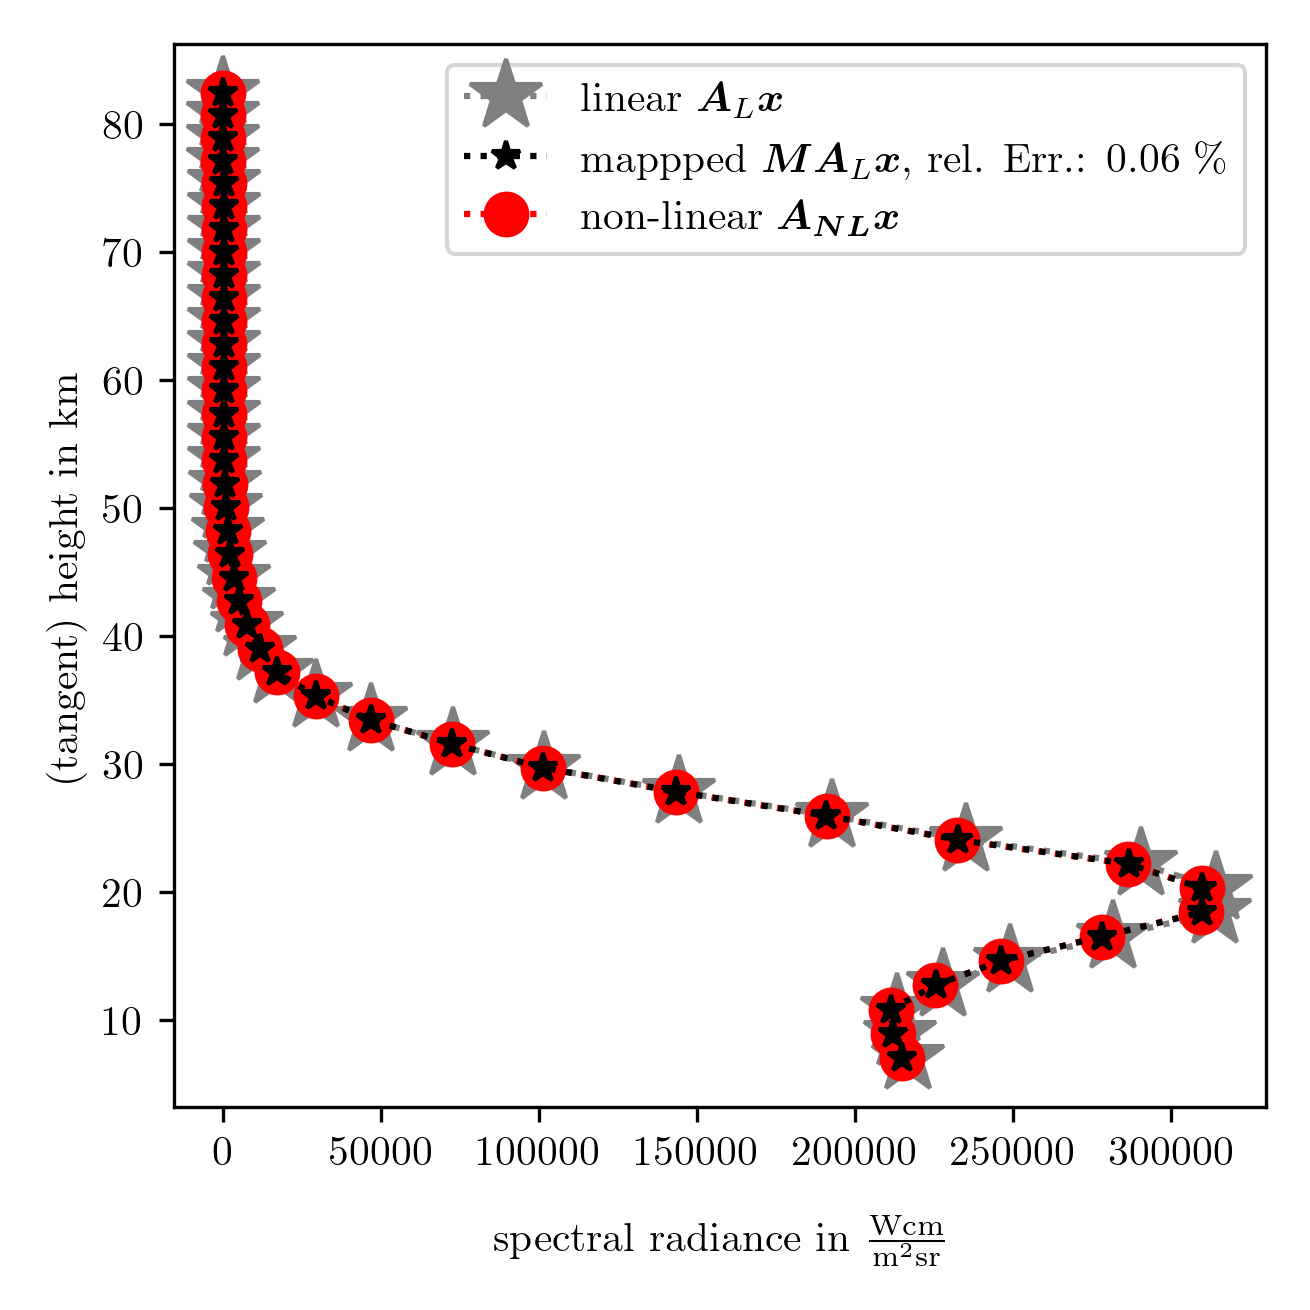
\includegraphics{SampMapAssesment.png}
	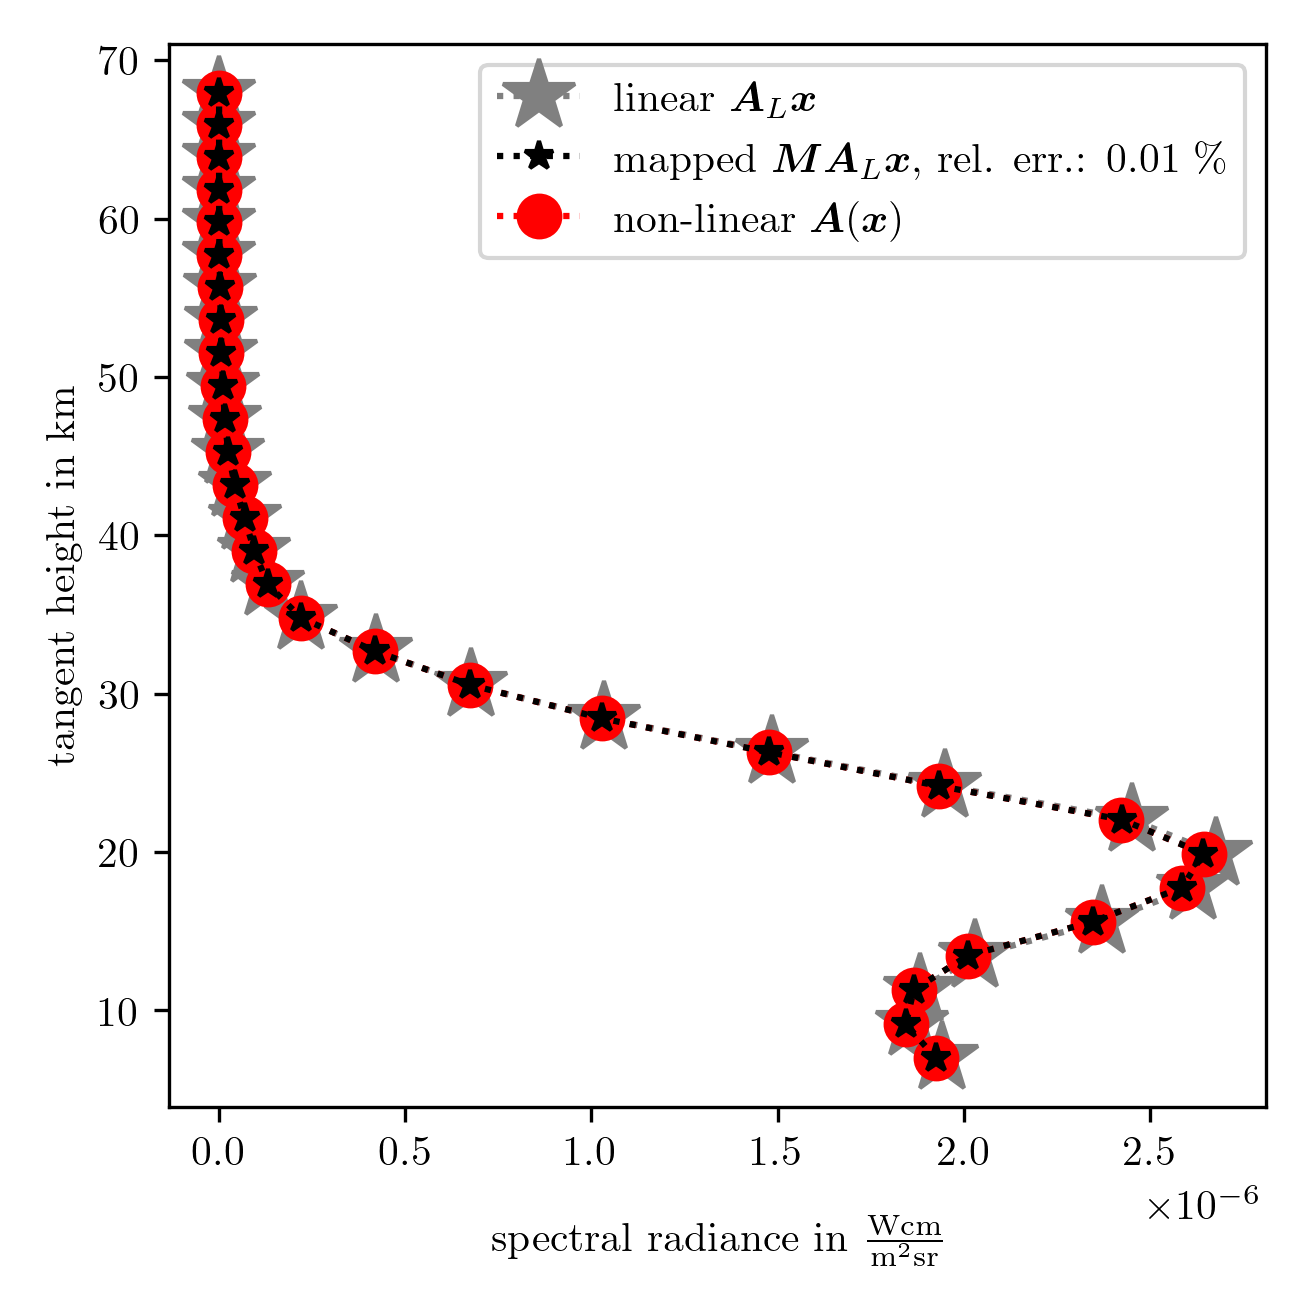
\includegraphics{SampMapAssesmentTT.png}
	\caption[Assessment of affine map.]{Assessment of how well we can approximate noise-free non-linear data $\bm{A}(\bm{x})$  (red circles) with noise-free linear data $\bm{A}_L\bm{x}$ (grey stars) and the previously calculated affine map $\bm{M}$. The approximated noise-free data (black stars) has a relative RMS error of $\approx 0.06\%$ compared to the true non-linear noise-free data.
		The ozone sample to generate this noise-free data has not been used to create the affine map.}
	\label{fig:MapAsses}
\end{figure}
Fig.~\ref{fig:MapAsses} shows the mapping for one posterior ozone sample with a relative RMS error $\approx0.06\%$.
This posterior ozone sample has not been used to create this mapping; in other words, this is an unseen event not occurring in the training data.
Consequently, from here onwards, we use the approximated forward map.
\section{Marginal and then Conditional Posterior -- Ozone}

Again, we use the MTC scheme and the exact same setup and procedure as in Sec. \ref{sec:FirstO3Post} to evaluate the marginal posterior and then the full conditional posterior of ozone with similar computational time.

\begin{figure}[ht!]
	\centering
	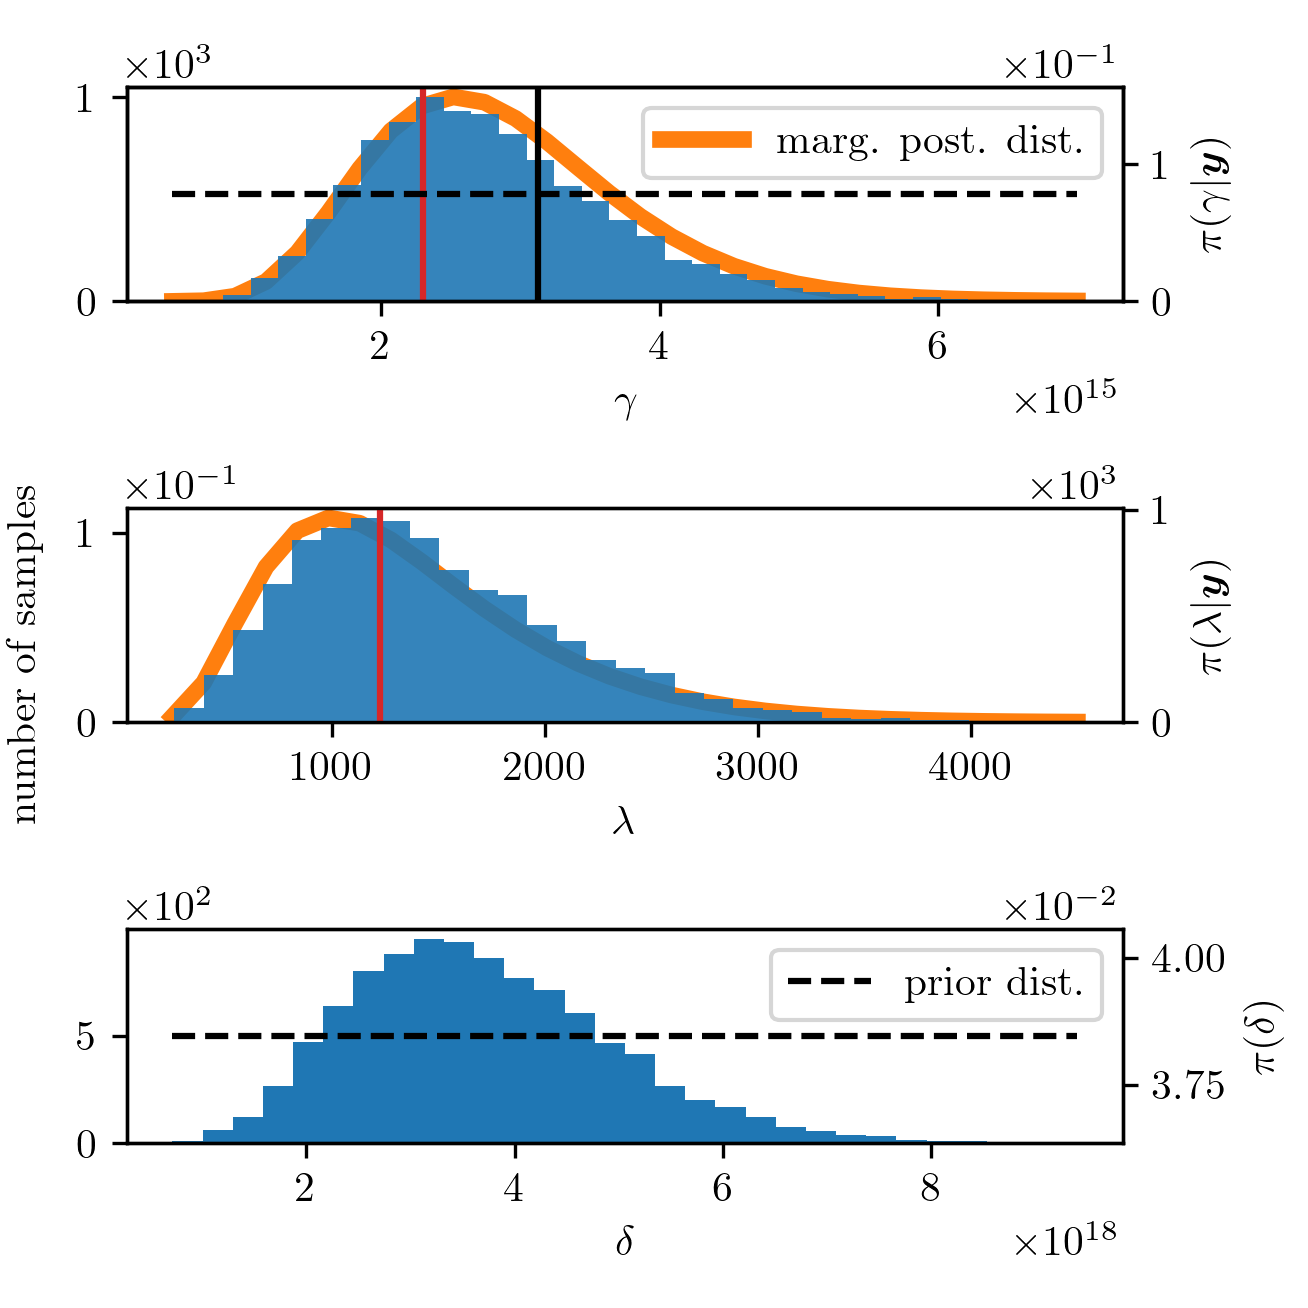
\includegraphics{secMargO3Res.png}
	\caption[Marginal posterior histograms and TT approximation as well as hyper-prior distribution.]{The TT approximation of the marginal posterior in orange and the samples as a histogram, as well as the prior distribution with a dotted line. We sample $\lambda$ and $\gamma$ using the MWG algorithm and then calculate $\delta$ for every sample of the marginal posterior. The regularised parameter corresponding to the best regularised solution (see Fig.~\ref{fig:O3SolplsReg} and Fig.~\ref{fig:LCurve}) is marked with the red vertical line. We mark the ground truth noise precision with the back vertical line.}
	\label{fig:MargPostHistTT}
\end{figure}
The marginal posterior is defined as in Eq.~\ref{eq:MargPostAppl}, but with the approximated forward model.
The MWG is initialised at the mode of $\pi(\lambda,\gamma| \bm{y})$ and $f(\lambda)$ and $g(\lambda)$ are approximated around the mode as in Sec. \ref{subsec:FirstMargPost} (see Eq.~\ref{eq:fAprox} and Eq.~\ref{eq:gAprox}).
We take $N = 10000$ plus $N_{\text{burn-in}} = 100$ steps in $\approx 0.5$s.
The IACTs provided by~\cite{drikHesse} are $\tau_{\text{int}, \gamma} \approx 5.2 \pm 0.3$ and $\tau_{\text{int}, \lambda} = 11 \pm 1 $ (see Fig. \ref{fig:IATCSecO3gam} and Fig.~\ref{fig:IATCSecO3lam}) and similar to the previously calculated values.
We plot the samples in Fig. \ref{fig:MargPostHistTT} as well as the TT approximation of the marginal posterior using 400 function evaluations (same grid; same number of ranks; see Sec.~\ref{subsec:FirstMargPost}).
The relative RMS error of the TT approximation over the whole grid and the relative RMS approximation error of $\pi(\lambda,\gamma| \bm{y})$ due to the approximations of $f(\lambda)$ and $g(\lambda)$ are both $\approx 8 \%$.

\begin{figure}[ht!]
	\centering
	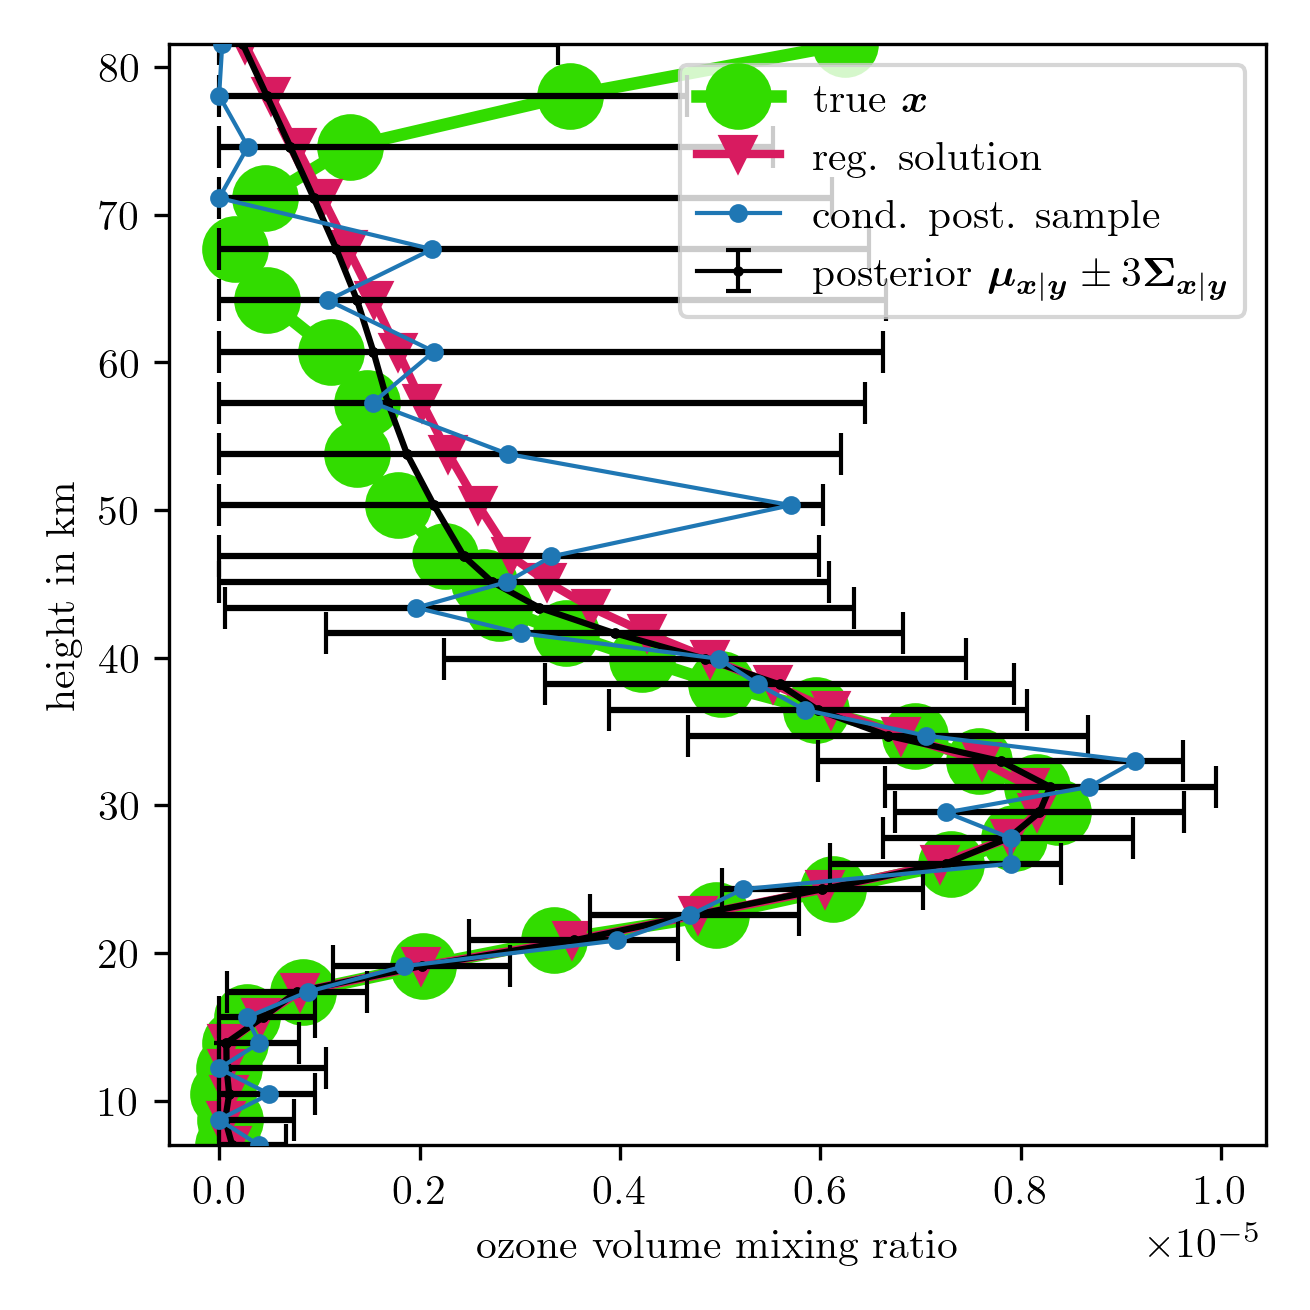
\includegraphics{SecRecResinclRegandSampl.png}
	%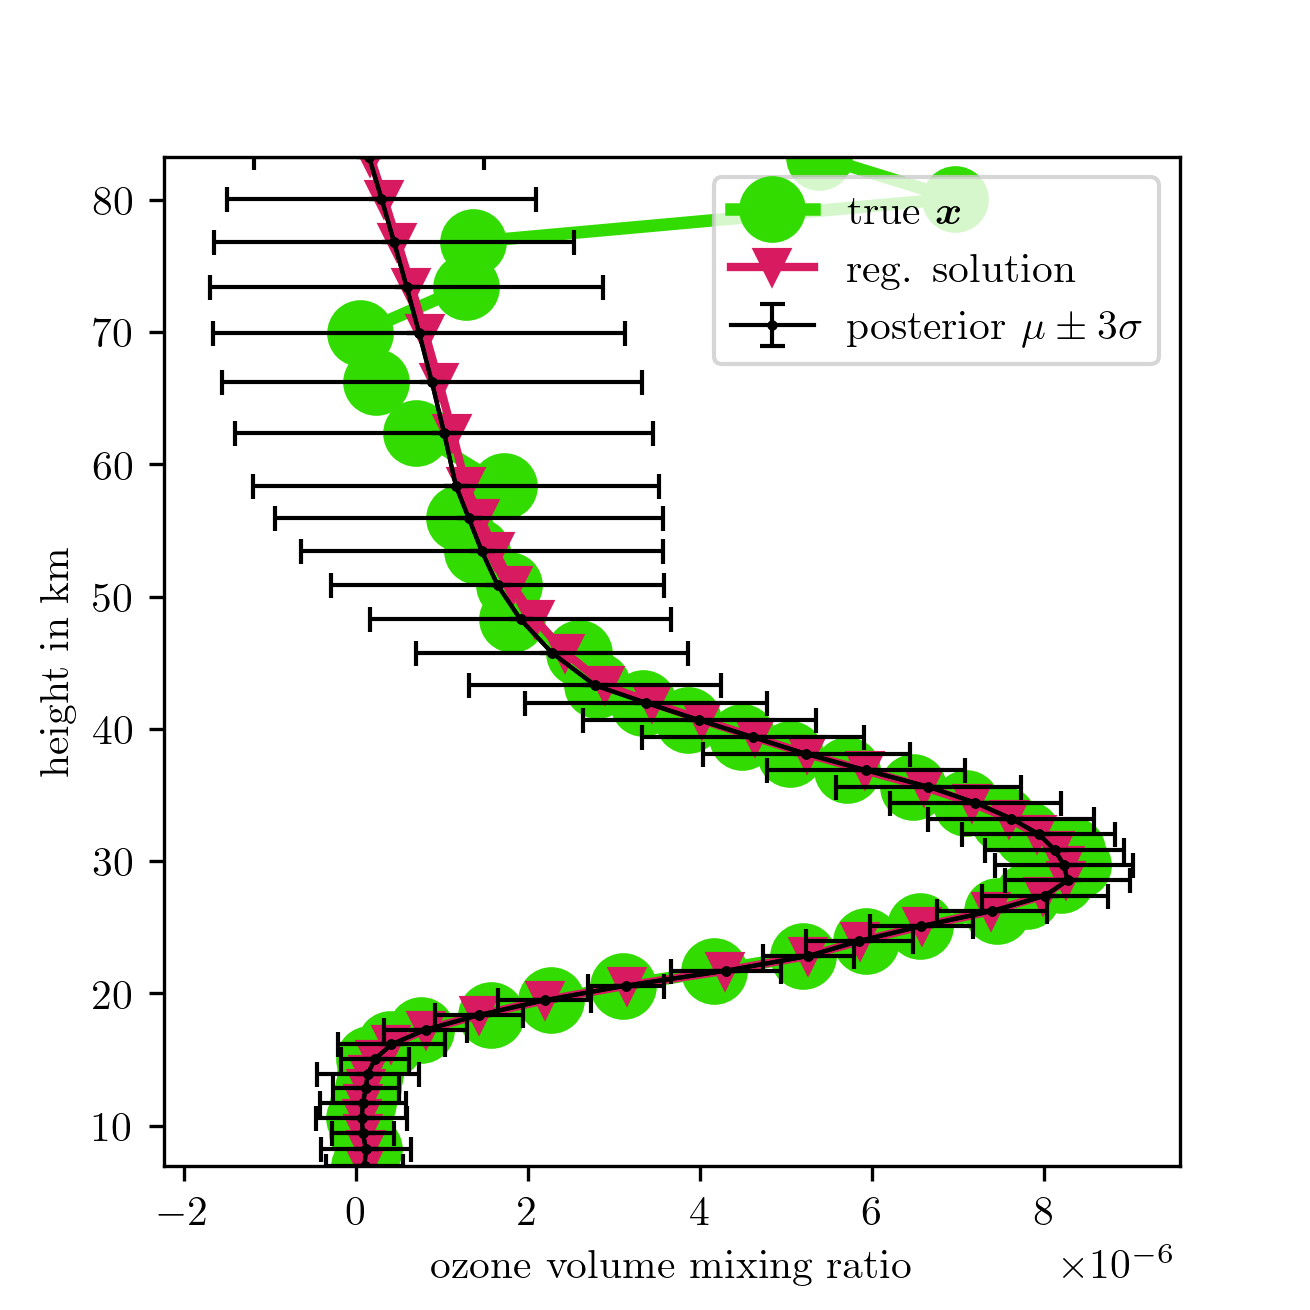
\includegraphics{SecRecResinclReg.png}
	\caption[Full posterior mean and variance of ozone and the regularised solution compared to the ground truth.]{Full posterior mean and variance and one ozone sample from the full posterior. We plot the regularised solution on top of the ground truth ozone profile in green. The results are based on the approximated forward model $\bm{M}\bm{A}_L$.}
	\label{fig:O3SolplsReg}
\end{figure} 
Again, we calculate the full posterior mean $\bm{\mu}_{\bm{x}|\bm{y}}$, see Eq.~\ref{eq:MeanInt}, and covariance matrix $\bm{\Sigma}_{ \bm{x}|\bm{y}}$~\ref{eq:CovInt} as weighted expectation.
We plot the results and one sample of $\pi(\bm{x}|\bm{y})$, which represents a feasible solution to this inverse problem, in Fig.~\ref{fig:O3SolplsReg}, as well as the regularised solution (see next section), and one sample from the posterior.
We can see that the ground truth lies within the STD around the mean, except for the peak at around $80$km.
Compared to the previously calculated mean and variance based on the linear forward model $\bm{A}_L$ (see \ref{fig:O3Samp}), the posterior distribution based on $\bm{M A}_L$ does not differ significantly.
This is expected since the difference between the linear and non-linear forward map of $\approx 1 \%$ is small.
%\clearpage


%Then we are able to define a linear model $ \bm{A} \coloneqq \bm{M} \bm{A}_{L}$, which approximates the non-linear model.
%Here, we give a brief introduction to affine maps.
%
%An affine map is any linear map between two vector spaces or affine spaces, where an affine space does not need to preserve a zero origin (see~\cite[Def. 2.3.1]{berger2009geometry}). \textcolor{red}{no it's not}
%In other words, an affine map does not need to map to the origin of the associated vector space.
%An affine map is a linear map on vector spaces, including a translation, or, in the words of my supervisor, C. F., a Taylor series of first order. \textcolor{red}{it is not a linear map , the origin of the domain to the origin of the range, fix this sentence - -it makes no sense.}
%For more information on affine spaces and maps, we refer to the books~\cite{berger2009geometry, katsumi1994affine}. \textcolor{red}{don't say that, say that it is a linear map plus a constant.}
%
%\textcolor{red}{these are horrible books. No wonder you have a garbled idea and description. All affine maps look like y = Ax+b where A is linear and b is a constant. What's so difficult about that?
%	I asked a LLM:
%	Please give a simple definition of an affine map (between two vector spaces)
%	Sure! A simple definition of an affine map between two vector spaces is:
%	An affine map is a function between vector spaces that preserves straight lines and has the form
%	$>f(x)=Ax+b>$
%	where A is a linear transformation and b is a fixed vector.
%	So it’s like a linear map, but with a shift. }
\chapter{Joint Retrieval of Ozone, Pressure and Temperature}
\label{ch:FullBay}
\thispagestyle{empty}
Here we extend the hierarchical Bayesian model set up in Sec. \ref{sec:BayModelO3} to include pressure and temperature related hyper-parameters and elaborate on some aspects of prior modelling.
The MTC scheme is applied to jointly provide posterior distributions of ozone, pressure and temperature.
Additionally, the reader is guided through the process of setting up an efficient TT approximation of the higher-dimensional marginal posterior.



\section{Hierarchical Bayesian Framework}
\label{sec:FullHierarch}
\begin{figure}[thb!]
	\centering
	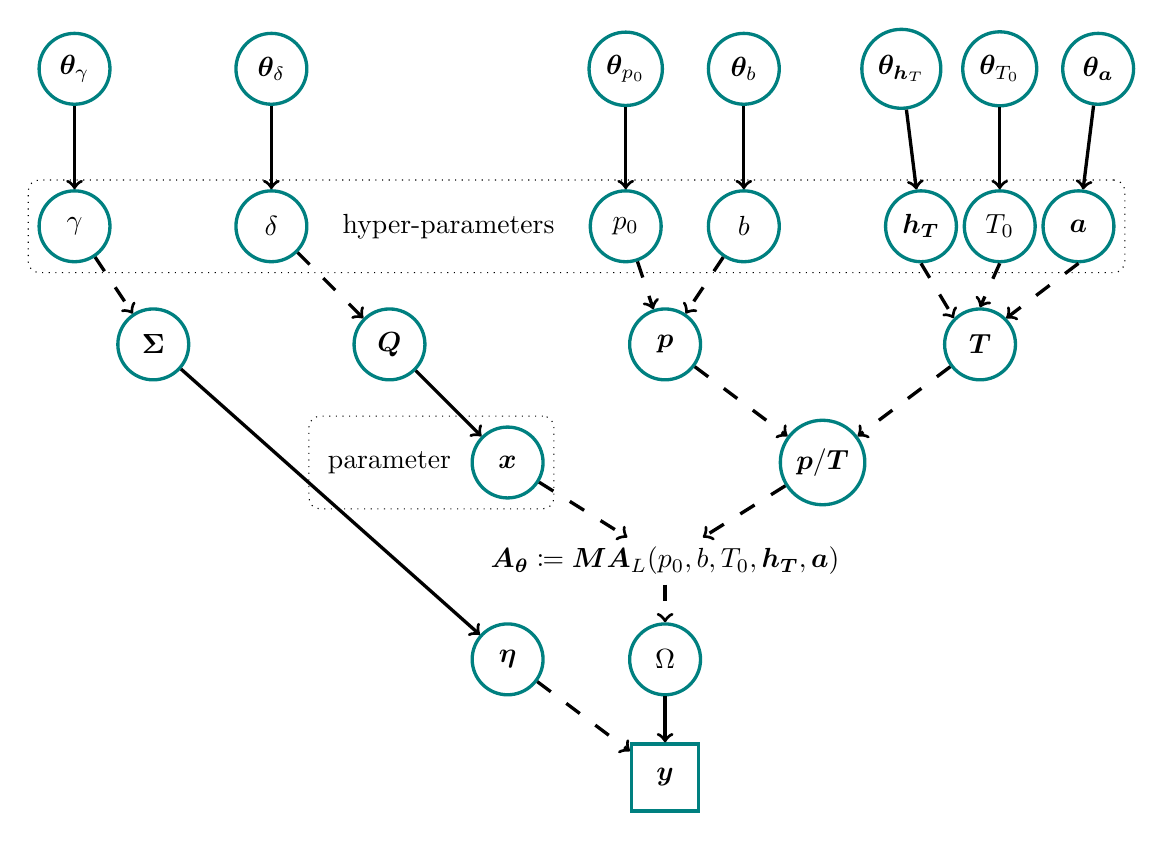
\begin{tikzpicture}
		\node[roundnode2] at (-4.5,6.5) (Q)     {$\bm{Q}$};
		\node[roundnode2] at (-3,5) (x)     {$\bm{x}$};
		\node[align=center] at (-1,3.75) (A)    {$\bm{A}_{\bm{\theta}} \coloneqq \bm{M}\bm{A}_L(p_0,b,T_0,\bm{h_T},\bm{a})$};
		\node[roundnode2] at (-1,2.5) (u)    {$\Omega$};
		\node[rectnode] at (-1,1) (y)    {$\bm{y}$};
		\node[roundnode2] at (-3,2.5) (e)    {$\bm{\eta}$};
		\node[roundnode2] at (-7.5,6.5) (S)    {$\bm{\Sigma}$};
		\node[roundnode2] at (-8.5,8) (s)    {$\gamma$};
		\node[roundnode2] at (-6,8) (d)    {$\delta$};
		\node[roundnode2] at (3,6.5) (t)     {$\bm{T}$};
		\node[roundnode2] at (-1,6.5) (p)     {$\bm{p}$};
		\node[roundnode2] at (1,5) (pt)     {$\bm{p}/\bm{T}$};
		\node[roundnode2] at (0,8) (b1)    {$b$};
		%\node[roundnode2] at (1,8) (b2)    {$b_2$};
		%\node[roundnode2] at (-2,8) (h1)    {$h_{0}$};
		\node[roundnode2] at (-1.5,8) (p0)    {$p_0$};
		\node[roundnode2] at (2.25,8) (ht)    {$\bm{h_T}$};
		\node[roundnode2] at (3.25,8) (ct)    {$T_0$};
		\node[roundnode2] at (4.25,8) (at)    {$\bm{a}$};
		
		\node[roundnode2] at (0,10) (b1hyp)    {$\bm{\theta}_{b}$};
		%\node[roundnode2] at (-2.5,10) (h1hyp)    {$\bm{\theta}_{h_{0}}$};
		\node[roundnode2] at (-1.5,10) (p0hyp)    {$\bm{\theta}_{p_{0}}$};
		\node[roundnode2] at (2,10) (hthyp)    {$\bm{\theta}_{\bm{h}_T}$};
		\node[roundnode2] at (3.25,10) (cthyp)    {$\bm{\theta}_{T_{0}}$};
		\node[roundnode2] at (4.5,10) (athyp)    {$\bm{\theta}_{\bm{a}}$};
		
		\node[roundnode2] at (-8.5,10) (shyp)    {$\bm{\theta}_{\gamma}$};
		\node[roundnode2] at (-6,10) (dhyp)    {$\bm{\theta}_{\delta}$};
		
		%Lines
		
		
		\draw[->, very thick] (S) -- (e);
		\draw[->, mydotted, very thick] (s) -- (S);
		\draw[->, very thick] (u) -- (y);
		\draw[->, mydotted, very thick] (A) -- (u);
		\draw[->, mydotted,  very thick] (x) -- (A);
		\draw[->, mydotted, very thick] (p) -- (pt);
		\draw[->, mydotted, very thick] (t) -- (pt);
		\draw[->, mydotted, very thick] (pt) -- (A);
		%\draw[->, mydotted, very thick] (h1) -- (p);
		\draw[->, mydotted, very thick] (p0) -- (p);
		\draw[->, mydotted, very thick] (b1) -- (p); 
		%\draw[->, very thick] (b2.south) -- (p.east); 
		\draw[->, mydotted, very thick] (d) -- (Q); 
		\draw[->, mydotted, very thick] (e) -- (y); 
		
		\draw[->, very thick] (Q.south east) -- (x.north west); 
		\draw[->, mydotted, very thick] (ht.south) -- (t.north west);
		\draw[->, mydotted, very thick] (ct.south) -- (t.north);
		\draw[->, mydotted, very thick] (at.south) -- (t.north east);
		
		
		\draw[->, very thick] (b1hyp) -- (b1);
		%\draw[->, very thick] (h1hyp) -- (h1);
		\draw[->, very thick] (p0hyp) -- (p0);
		\draw[->, very thick] (hthyp) -- (ht);
		\draw[->, very thick] (cthyp) -- (ct);
		\draw[->, very thick] (athyp) -- (at);
		\draw[->, very thick] (shyp) -- (s);
		\draw[->, very thick] (dhyp) -- (d);
		
		\node[fit=(s)(at),draw,dotted,black, rounded corners] {};
		\node[align =center] at (-3.75,8) (T1) {hyper-parameters};
		\node[align =center] at (-4.5,5) (T2) {parameter};
		\node[fit=(x)(T2),draw,dotted,black, rounded corners] {};
		
	\end{tikzpicture} 
	\caption[Directed acyclic graph of Bayesian model for ozone $\bm{x}$, pressure $\bm{p}$ and temperature $\bm{T}$.]{DAG of the hierarchical Bayesian model including ozone $\bm{x}$, pressure $\bm{p}$ and temperature $\bm{T}$. The hyper-parameters $\bm{h}_T= \{ h_{T,1}, h_{T,2},h_{T,3},h_{T,4},h_{T,5},h_{T,6}\}$, $\bm{a} = \{ a_0, a_1, a_2,a_3,a_4,a_5,a_6\}$, $T_0$, $b$ and $p_0$ deterministically (dotted line) describe pressure through Eq.~\ref{eq:pressFunc} and temperature through Eq.~\ref{eq:tempFunc}. In this case, the hyper-parameters $\pi(p_0,b,T_0,\bm{h_T},\bm{a})$ are a normally distributed a-priori. That is why $\bm{\theta}_{\bm{h}_T},\bm{\theta}_{\bm{a}}, \bm{\theta}_{T_{0}},\bm{\theta}_{b} , \bm{\theta}_{p_0}$ represent mean and variances e.g.,~$b \sim \mathcal{N}(\mu_b, \sigma^2_b)$ and $\bm{\theta}_{b} = \{\mu_b, \sigma_b\}$.
	 As previously described in Sec.~\ref{sec:BayModelO3}, $\bm{\theta}_{\gamma}, \bm{\theta}_{\delta}$ determine gamma distributions e.g., $\gamma \sim \Gamma(\alpha_{\gamma},\beta_{\gamma}) $ with $\bm{\theta}_{\gamma} = 	\{\alpha_{\gamma},\beta_{\gamma} \}$.
	The ozone parameter $\bm{x}$ is statistically (solid line) described by the prior distribution $\bm{x}| \delta \sim \mathcal{N}(0,(\delta \bm{L})^{-1}) $. 
	Here, the hyper-parameter $\delta$ accounts for smoothness in the ozone profile and defines the precision matrix $\bm{Q} = \delta \bm{L}$, where $\bm{L}$ is the graph Laplacian as in Eq.~\ref{eq:GLapl}.
	The noise covariance $\bm{\Sigma} = \gamma^{-1} \bm{I}$ of the random noise vector $\bm{\eta} \sim \mathcal{N}(0,\gamma^{-1} \bm{I} ) $ is defined by the hyper-parameter $\gamma$.
	From the space of all measurables $\Omega$ mapped through the approximated forward model $\bm{A}_{\bm{\theta}} \coloneqq \bm{M}\bm{A}_L(p_0,b,T_0,\bm{h_T},\bm{a})$, depending on the hyper-parameter $\bm{\theta}  \coloneqq \{p_0, b, T_0,\bm{h}_T,\bm{a} \}$ a data set $\bm{y}$ is randomly observed (square box) including some additive random noise $\bm{\eta}$.}
	%Given the data we like to determine the marginal posterior distribution over the hyper-parameters $\pi(\bm{\theta}, \delta, \gamma | \bm{y})$ first and then the conditional posterior distribution for ozone $\pi(\bm{x}|\bm{\theta}, \delta, \gamma, \bm{y})$, utilising the MTC scheme.}
	\label{fig:DAGComplete}
\end{figure}
As in Sec.~\ref{sec:BayModelO3}, the DAG in Fig.~\ref{fig:DAGComplete} visualises the measurement process and conditional dependencies between the parameter and the hyper-parameters.
Ozone $\bm{x}$, pressure $\bm{p}$ and temperature $\bm{T}$ progress deterministically (dashed line) into the forward model, via $\bm{x} \times \bm{p} / \bm{T}$.
Note that other variables in the RTE, such as the internal partition function and the black body radiation, are dependent on temperature (see Sec.~\ref{sec:RTE}).
This hierarchical Bayesian framework includes the hyper-parameters $p_0, b$ for pressure (see Eq.~\ref{eq:pressFunc}), $\bm{a}, \bm{h}_T, T_0$ for temperature (see Eq.~\ref{eq:tempFunc}), $\delta$ for ozone smoothness and $\gamma$ for noise precision.
Each of those hyper-parameters is described by the hyper-prior distribution $\pi(p_0,b,T_0,\bm{h_T},\bm{a}, \delta,\gamma)$ (see Sec.~\ref{subsec:PriorFull}).
Through their respective prior distributions, pressure $\bm{p}$, temperature $\bm{T}$ and ozone $\bm{x}$ generate a space of all possible noise-free data $\Omega$ from which some data with additive normally distributed noise $\bm{\eta}$ is observed.
For brevity, we define the linear forward model matrix as
\begin{align}
	\bm{A}_{\bm{\theta}} \coloneqq \bm{M}\bm{A}_L(p_0,b,T_0,\bm{h_T},\bm{a}) 
\end{align}
with $\bm{\theta}  \coloneqq \{p_0,b,T_0,\bm{h_T},\bm{a}  \}$ accounting for the all pressure and temperature related hyper-parameters and $\bm{M}$ the affine approximation from the previous Chapter.

\clearpage
\noindent
The distributions of the hierarchical Bayesian framework are:
\begin{subequations}
	\label{eq:BayMode}
	\begin{align}
		\bm{y} |  \bm{x},\bm{\theta},\delta,\gamma  &\sim \mathcal{N}(\bm{A}_{\bm{\theta}}  \bm{x}, \gamma^{-1} \bm{I}) \label{eq:likelihoodFull} \\
		\bm{x}| \delta  &\sim \mathcal{N}(\bm{0}, (\delta \bm{L})^{-1} ) \label{eq:priorXFull} \\
		\delta  &\sim \Gamma(\alpha_{\delta} , \beta_{\delta} )\label{eq:priorDelFull} \\
		\gamma  &\sim \Gamma(\alpha_{\gamma}, \beta_{\gamma})\label{eq:priorGamFull} \\
		\bm{a}  &\sim \mathcal{N}(\bm{\mu}_{\bm{a}}, \bm{\Sigma}_{\bm{a}})\\
		\bm{h}_{\bm{T}}  &\sim \mathcal{N}(\bm{\mu}_{T}, \bm{\Sigma}_{\bm{h}_T}) \\
		T_0  &\sim \mathcal{N}(\mu_{T_0}, \sigma_{T_0} )\\
		p_0  &\sim \mathcal{N}(\mu_{p_0}, \sigma_{p_0} )\\
		b  &\sim \mathcal{N}(\mu_b, \sigma_b )  \label{eq:lastprior}  \, .
	\end{align}
\end{subequations}
Due to Gaussian noise $\pi(\bm{y} |  \bm{x},\bm{\theta},\delta,\gamma )$ is a normally distributed likelihood function and Eq.~\ref{eq:priorXFull} to Eq.~\ref{eq:lastprior} denote prior distributions.
Before formulating the posterior distribution, we carefully define $\bm{\theta}_{\gamma}, \bm{\theta}_{\delta},\bm{\theta}_{p_0},\bm{\theta}_{b},\bm{\theta}_{\bm{h}},\bm{\theta}_{T_0},\bm{\theta}_{\bm{a}}$, the hyper-prior scales, shapes, means and variances, which are explicitly given in Tab.~\ref{tab:priors}.

\subsection{Prior Modelling}
\label{subsec:PriorFull}
\begin{figure}[ht!]
	\centering
	\input{TrueTemp.pdf_tex}
	%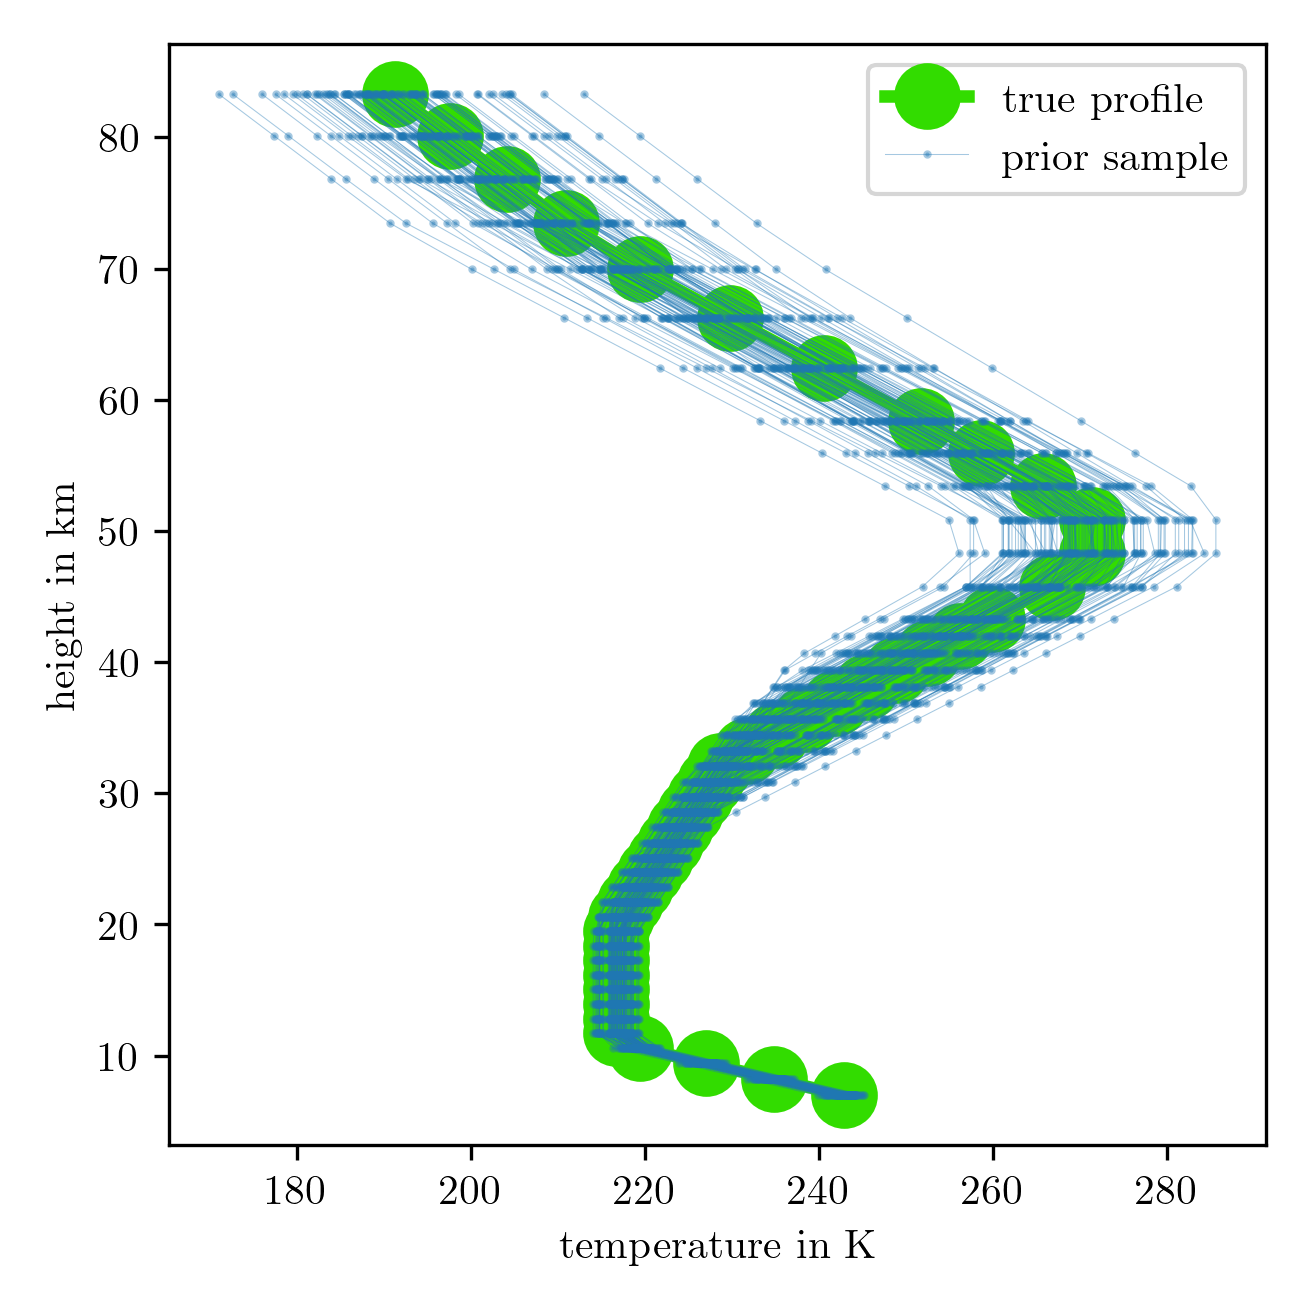
\includegraphics{PriorTempPostMeanSigm.png}
	\caption[Prior Samples of $\bm{T}$ according to the respective hyper-prior distribution.]{Prior samples from the hyper-prior distribution of $\bm{h}_T$, $\bm{a}$ and $T_0$, as defined in Tab.~\ref{tab:priors}, where we calculate $\bm{T}$ according to the function in Eq.~\ref{eq:tempFunc}.}
	\label{fig:PriorTemp}
\end{figure}
\begin{figure}[ht!]
	\centering
	\input{TruePress.pdf_tex}
	%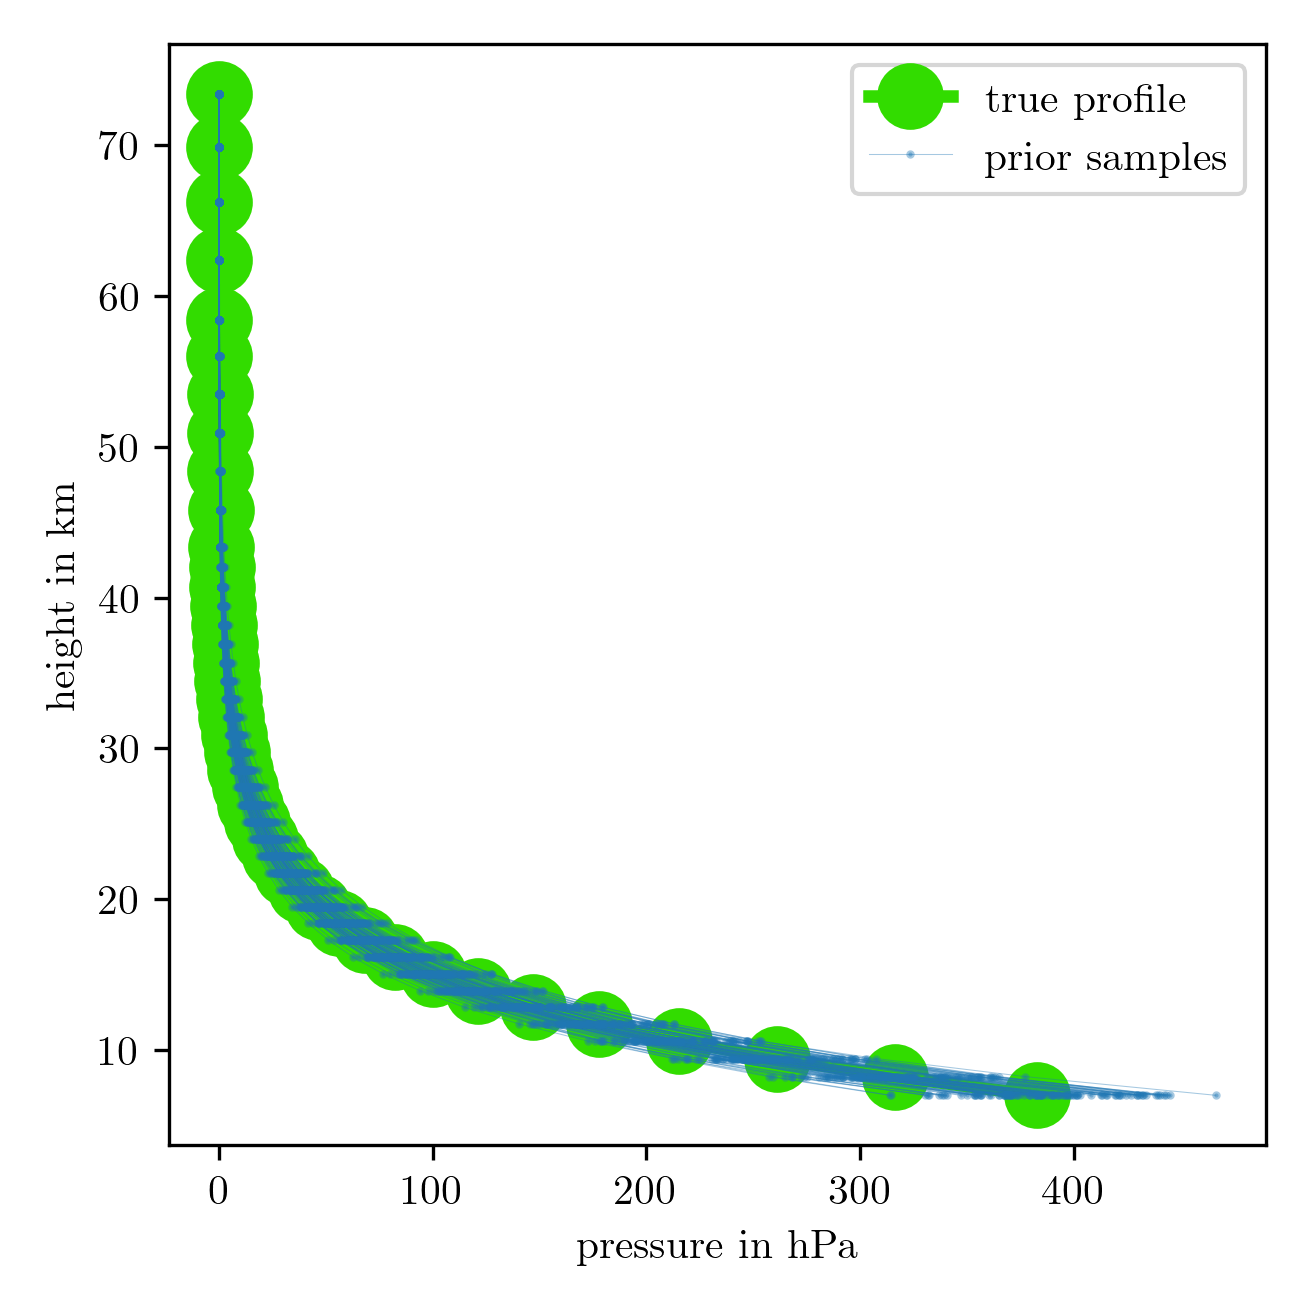
\includegraphics{PriorPressPostMeanSigm.png}
	\caption[Prior Samples of $\bm{p}$ according to the respective hyper-prior distribution.]{Prior samples from the hyper-prior distribution of $b$ and $p_0$ as defined in Tab.~\ref{tab:priors}, where we calculate $\bm{p}$ according to the function in Eq.~\ref{eq:pressFunc}.}
	\label{fig:PriorPress}
\end{figure}
\begin{figure}[ht!]
	\centering
	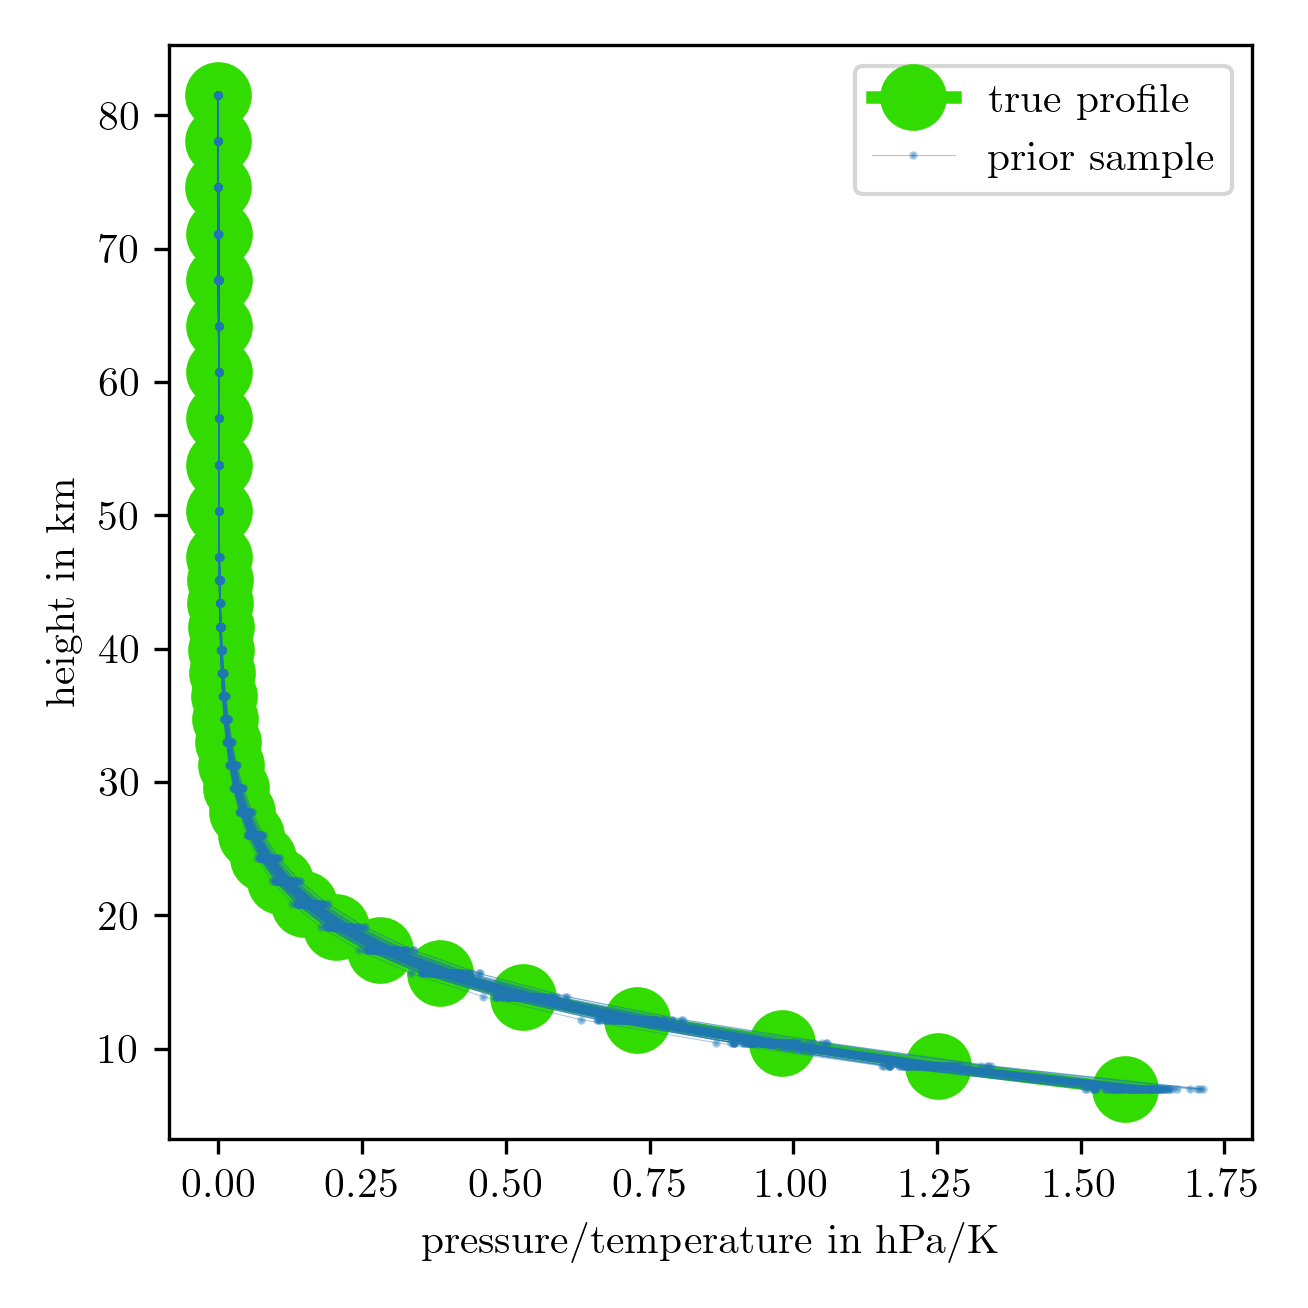
\includegraphics{PriorTempOverPostMeanSigm.png}
	\caption[Prior Samples of $\bm{p}/\bm{T}$ according to the respective hyper-prior distribution.]{Prior samples from the hyper-prior distribution of $\bm{h}_T$, $\bm{a}$ and $T_0$ for temperature as in Eq.~\ref{eq:tempFunc} and $b$ and $p_0$ for pressure as in Eq.~\ref{eq:pressFunc}. We plot $\bm{p}/\bm{T}$. The hyper-priors are defined in Tab.~\ref{tab:priors}.}
	\label{fig:PriorPressOverTemp}
\end{figure}
We observe that the pressure $\bm{p}$ in between $h_{L,0} \approx 7$km and $h_{L,n} \approx 83$km can be described with an exponential function
\begin{align}
	p(h) =
	\exp \left( -b \, h \right)   \,  p_0 \quad , \text{$h_{L,0}  \leq h \leq h_{L,n}$}
	\label{eq:pressFunc}
\end{align}
depending on two hyper-parameters $p_0,b$ (see Fig.~\ref{fig:PriorPress}).
Similarly, the temperature as described in Eq.~\ref{eq:tempFunc} can be parametrised with 14 hyper-parameters\linebreak $\bm{h}_T = \{ h_{T,1}, h_{T,2},h_{T,3},h_{T,4},h_{T,5},h_{T,6} \}$, $\bm{a} = \{a_0, a_1, a_2,a_3,a_4,a_5,a_6 \} $ and $T_0$ (see Fig.~\ref{fig:PriorTemp} and Eq.~\ref{eq:tempFunc}).

The hyper-prior distributions for $p_0,b, T_0,\bm{h}_T ,\bm{a} $ are defined to be Gaussians, and to complete the model we have to set sensible hyper-prior variances and means.
We tune the variances of $\pi(\bm{h}_T)$, so that the temperature profile maintains its structure and $ h_{T, i} < h_{T, i+1}$, for $i = 1,\dots, 5$ (see Fig.~\ref{fig:HeightPriors}).
The means of $\pi(\bm{h}_T)$ and $\pi(\bm{a})$ are set to ground truth values see Tab.~\ref{tab:tempGrad} and the variances of $\pi(\bm{a})$ allow a wide range of prior temperature profiles.
Similarly, we set the variance and mean of $\pi(T_0)$ so that it mimics a daily temperature variability of roughly $30$K around the mean sea level temperature $288$K~\cite{atmosphere1976us}.
These hyper-prior distributions are rather informative, because we find that the data and the model (see Fig.~\ref{fig:PriorPressOverTemp}) are uninformative about the temperature profile.
The variance of $\pi(b)$ is set to a rather large value.
The variability of $\pi(p_0)$ is $\approx 80$hPa and close to what we can observe when looking at weather data.
Means for $\pi(b ,p_0)$ are provided by fitting the exponential in Eq.~\ref{eq:pressFunc} to ground truth pressure values via the Python function \texttt{scipy.optimize.curve\_fit}.
The in Sec.~\ref{subsec:PriorModelO3} defined Gamma distributions $\pi(\delta,\gamma)$ are not changing.
See Tab.~\ref{tab:priors} for a summary of the hyper-prior distributions.

Prior samples of the pressure $\bm{p}$ in Fig.~\ref{fig:PriorPress}, the temperature $\bm{T}$ in Fig.~\ref{fig:PriorTemp}, the ratio $\bm{p}/\bm{T}$ in Fig.~\ref{fig:PriorPressOverTemp} and additionally prior samples of $1/\bm{T}$ in Fig.~\ref{fig:OverTempPrior} are plotted against their ground truth profiles.
Here we already observe that $\bm{p}/\bm{T}$ inherits the structure of the pressure function and hence the model is uninformative about the temperature.
\clearpage
%Note that we fit one exponential function to ground truth pressure values between $h_{L,0} \approx 7$km and $h_{L,n} \approx 82$, so that the pressure value $p_0$ may be different to true sea-level pressure values at $h = 0$km due to that approximation.
\section{Posterior Distribution}
Here the marginal and then the full conditional posterior distribution for the described Bayesian model are formulated.
We either use the t-walk algorithm~\cite{christen2010general} to draw samples from $\pi(p_0,b,T_0,\bm{h_T},\bm{a} ,\lambda, \gamma| \bm{y})$ with $\lambda = \delta / \gamma$ or we utilise a TT approximation on a predefined grid to generate samples via the SIRT method with an MH correction step.
In doing so, the reader is guided through the process of obtaining an efficient TT approximation and some key aspects are pointed out.
Lastly, the RTO method is utilised to draw ozone samples from the full conditional posterior $\pi(\bm{x}|p_0,b,T_0,\bm{h_T},\bm{a} ,\lambda, \gamma, \bm{y})$.
Recall that the linear forward model matrix is $\bm{A}_{\bm{\theta}}$ is depending on the hyper-parameter defined as $\bm{\theta}  \coloneqq \{p_0,b,T_0,\bm{h_T},\bm{a}  \}$.
\begin{table}[ht!]
	\centering
	\begin{tabular}{ |c||c|c|c|c|c|   }
		\hline
		& &\multicolumn{2}{|c|}{TT bounds}& t-walk&\\
		\hline
		model parameters& priors&\makecell{lower}& \makecell{upper\\
		}&$\tau_{\text{int}}$&Context\\
		\hhline{|=||=|=|=|=|=|}
		$\bm{x}$ &$\mathcal{N}(0,(\delta \bm{L})^{-1})$ & -&-&-& $\bm{x}$\\ \hline
		$\delta$ &$\mathcal{T}(1,10^{-35})$ & -&-&  -& $\bm{x}$\\ \hline
		$\gamma$ & $\mathcal{T}(1,10^{-35})$ &$8\times10^{14}$ &$1.2\times10^{16}$&  $ 507\pm 29$ &$\bm{y}$\\ \hline
		$\lambda  = \delta / \gamma$ &- & $1\times10^{-5}$&$2.5\times10^{-3}$& $979 \pm 75$ & -\\ \hline
		$b$ &  $\mathcal{N}(0.174,(0.01)^2)$& 0.129& 0.214 &$830\pm 60$&$\bm{p}$\\ \hline
		$h_{T,1}$ &  $\mathcal{N}(11,(1.5)^2)$&5.4 &16.3&$286\pm 13$ &$\bm{T}$\\ \hline
		$T_{0}$ &  $\mathcal{N}(288.15,(10)^2)$& 247 &326&$279 \pm 12$&$\bm{T}$\\ \hline
		$p_0$ &  $\mathcal{N}(1311,(20)^2)$&1237 &1387&$279\pm 12$&$\bm{p}$\\ \hline
		$h_{T,3}$ &  $\mathcal{N}(32.3,(2.5)^2)$&22.9&41.7&$254\pm 11$&$\bm{T}$\\ \hline
		$a_{1}$ &  $\mathcal{N}(0,(0.1)^2)$&-0.38 &0.38&$295 \pm 13$&$\bm{T}$\\ \hline
		$h_{T,2}$ &  $\mathcal{N}(20.1,(0.7)^2)$&17.2 &22.7&$296\pm 13$&$\bm{T}$\\ \hline
		$a_{0}$ &  $\mathcal{N}(-6.5,(0.01)^2)$&-6.54 &-6.47&$252 \pm 10$&$\bm{T}$\\ \hline
		$a_{2}$ &  $\mathcal{N}(1,(0.01)^2)$&0.97 &1.03&$267 \pm 11$&$\bm{T}$\\ \hline
		$a_{3}$ &  $\mathcal{N}(2.8,(0.1)^2)$&2.5 &3.1&$267\pm 11$&$\bm{T}$\\ \hline
		$h_{T,4}$ &  $\mathcal{N}(47.4,(0.5)^2)$&45.5 &49.3&$270 \pm 12$&$\bm{T}$\\ \hline
		$a_{4}$ &  $\mathcal{N}(0,(0.1)^2)$&-0.38 &0.38&$254 \pm 11$&$\bm{T}$\\ \hline
		$h_{T,5}$ &  $\mathcal{N}(51.4,(0.5)^2)$&49.5 &53.3&$280 \pm 12$&$\bm{T}$\\ \hline
		$a_{5}$ &  $\mathcal{N}(-2.8,(0.1)^2)$&-3.18 &-2.43&$278 \pm 12$&$\bm{T}$\\ \hline
		$h_{T,6}$ &  $\mathcal{N}(71.8,(3)^2)$&60.5 &83.1&$250\pm 10$&$\bm{T}$\\ \hline
		$a_{6}$ & $\mathcal{N}(-2,(0.01)^2)$ &-2.04 &-1.96&$272\pm 12$&$\bm{T}$\\
		\hline
	\end{tabular}
	\caption[Summary of relevant parameter characteristics, bounds and sampling statistics.]{Summary of relevant parameter and hyper-parameters bounds and statistics, ordered as in the TT format according to their correlation structure. We denote $\mathcal{N}(\mu= \text{mean},\sigma^2= \text{variance})$ as the Gaussian and $\mathcal{T}(\alpha = \text{scale}, \beta = \text{rate})$ as the Gamma distribution. The IACT $\tau_{\text{int}}$ from marginal posterior samples via the t-walk is twice the value provided by~\cite{UwerrM, drikHesse}.}
	\label{tab:priors}
\end{table}
\clearpage

\subsection{Marginal Posterior -- Pressure and Temperature}
The marginal posterior is given as
\begin{align}
	\pi( \bm{\theta},\lambda,\gamma  | \bm{y}) \propto &  \lambda^{n/2} \gamma^{m/2}   \exp{ \Bigl\{ - \frac{1}{2} g ( \bm{\theta},\lambda) - \frac{\gamma}{2} f (\bm{\theta},\lambda) \Bigr\}} \pi(\bm{\theta},\lambda,\gamma ) \, ,
	\label{eq:MargPostFull}
\end{align}
with $\lambda= \delta / \gamma$,
\begin{subequations}
	\label{eq:fandgTrue}
	\begin{align}
		&f ( \bm{\theta},\lambda) = \bm{y}^T \bm{y} - \big(\bm{A}_{\bm{\theta}}^T \bm{y}\big)^T \big(\bm{A}_{\bm{\theta}}^T  \bm{A}_{\bm{\theta}} + \lambda \bm{L}\big)^{-1} \big(\bm{A}_{\bm{\theta}}^T \bm{y}\big)  \label{eq:fFullAppl} \, ,  \\
		&\text{and } g(\bm{\theta},\lambda) = \log \det \big(\bm{A}_{\bm{\theta}}^T  \bm{A}_{\bm{\theta}} + \lambda \bm{L}\big) \label{eq:gFullAppl} \, .
	\end{align}
\end{subequations}
For each evaluation of $\pi( \bm{\theta},\lambda,\gamma  | \bm{y})$, $\bm{A}_{\bm{\theta}}$ is composed as in Chapter~\ref{ch:formodel}, and $f$ and $g$ are calculated directly using the Cholesky decomposition via the Python functions \texttt{np.linalg.cholesky} and \texttt{scy.linalg.cho\_solve}.

\subsubsection{Sampling from the marginal posterior}
Since the hierarchical model has $18$ hyper-parameters, we utilise the t-walk algorithm by Christen and Fox~\cite{christen2010general} to sample from the marginal posterior $\pi(\bm{\theta} , \lambda, \gamma| \bm{y})$, because it is quick-to-implement and easy-to-use.
The t-walk chooses between four different types of steps on the target distribution.
It is employed as a black-box algorithm in default settings, requiring the specification of the number of samples, burn-in period, support region, and the target distribution. 
Convergence to the target distribution is guaranteed by the construction of this algorithm~\cite{christen2010general}.

Running the t-walk~\cite{christen2010general} algorithm with the objective to generate $1000$ independent samples from the marginal posterior provides a ground truth to which we compare the TT approximation.
The maximum IACT provided by twice the value of \cite{wolff2004monte, drikHesse} (see Tab.~\ref{tab:priors} and Fig.~\ref{fig:TWalkIATC1} to Fig.~\ref{fig:TWalkIATC18}) can be bounded by $1100$.
Then the t-walk takes $N = 1000 \times 1100$ steps plus a burn-in period of $N_{\text{burn-in}} = 100 \times 1100 $ for $1000$ independent samples.
We initialise the Python implementation of the t-walk~\cite{christentwalkaccess} around the hyper-prior mean values and the mode of $\pi(\lambda ,\gamma|\bm{y})$ (see Sec.~\ref{subsec:MWG} and e.g., Fig.~\ref{fig:ScatterPlotTT}).
For a total number of $N + N_{\text{burn-in}} = 1210000$ steps within hyper-parameter support bounds given by the iteratively defined TT grid (see Tab.~\ref{tab:priors}) a time of $\approx 10$ mins is taken.
The resulting sample histograms are plotted in Fig.~\ref{fig:PostHistTT0} to Fig.~\ref{fig:PostHistTT4} and the trace of the samples in Fig.~\ref{fig:TraceTwalk}.
\begin{figure}[ht!]
	\centering
	\includegraphics{TraceTwalk.png}
	\caption[T-walk trace]{Output trace of samples from the marginal posterior distribution $\pi(\bm{\theta},\lambda,\gamma|\bm{y})$ via the t-walk.}
	\label{fig:TraceTwalk}
\end{figure}
\clearpage

\subsubsection{TT approximation of marginal posterior}
The aim now is to approximate the square root of the marginal posterior
\begin{align}
	\begin{split}
		\sqrt{\pi( \bm{\theta},\lambda,\gamma  | \bm{y})} \propto  \exp\Bigl\{ 0.5\log{\pi( \bm{\theta},\lambda,\gamma  | \bm{y}) } + c \Bigr\}  
	\end{split} 
	\label{eq:MargPostFullTT}
\end{align}
with a ``normalisation constant'' $c=-200$ to stay within computer precision.
In doing so, we run the~\texttt{tt.cross.rectcross.rect\_cross.cross} function from the \texttt{ttpy} python package \cite{Oseledets2018ttpy} on a grid (see Tab.~\ref{tab:priors}) according to the results of the t-walk.
When computing the marginal of each hyper-parameter as in Sec.~\ref{sec:tensortrain} the maximum values of $\sqrt{\pi( \bm{\theta},\lambda,\gamma  | \bm{y})}$ are around $10^{27}$ so we set $\xi = 1 / \uplambda (\mathcal{X})$ with $\uplambda(x) = 1$.
For Cartesian basis the mass matrix becomes $\bm{M}_k = \text{diag}(\uplambda_k(\mathcal{X}_k))$.
To draw samples from the TT approximation the SIRT-MH scheme is used as introduced in Sec. \ref{subsec:SamplTT}.

\paragraph{Correlation structure}
First, we order the hyper-parameters according to their correlation structure to improve the efficiency of the TT approximation of $\sqrt{\pi( \bm{\theta},\lambda,\gamma  | \bm{y})}$. 
Specifically, the hyper-parameter space $\mathcal{X}_{\gamma} \times \mathcal{X}_{\lambda} \times \mathcal{X}_{b} \times \cdots$ is arranged in such a way that highly correlated hyper-parameter pairs are adjacent and directly linked through their shared TT rank.
For samples via the SIRT-MH, twice the value of~\cite{wolff2004monte, drikHesse} provides an average IACT of $\approx 1.2 \pm 0.2$.
Hence 1000 independent samples from the marginal posterior require 2000 samples via the SIRT-MH scheme.
In Fig.~\ref{fig:CorrPlot} those 1000 samples and the Pearson correlation coefficients between hyper-parameter pairs are plotted.
A coefficient close to $1$ or $-1$ indicates strong correlation, while values near zero suggest weak or no correlation.
We observe that the hyper-parameters $\lambda$ and $b$, and $\lambda$ and $\gamma$ are highly correlated.
Additionally, $h_{T,1}$ describing the temperature at low altitudes (strong signal) is mildly correlated to $b$.
This is because $h_{T,1}$ influences ``the smoothness'' of $\bm{p}/\bm{T}$, which is hard to see in Fig.~\ref{fig:PriorPressOverTemp}.
Interestingly, $p_0$ appears largely uncorrelated with other hyper-parameters, while $b$ is the key parameter linking pressure to ozone and temperature.
Hyper-parameters describing the temperature at higher altitudes are very much uncorrelated and the IACTs of the t-walk in Tab.~\ref{tab:priors} agree with those results.
Alternatively, one could decorrelate the hyper-parameter space e.g.,~via Cholesky whitening~\cite{KessyWhitening2018}.


\clearpage
\begin{figure}[h!]% will be the left-side figure
	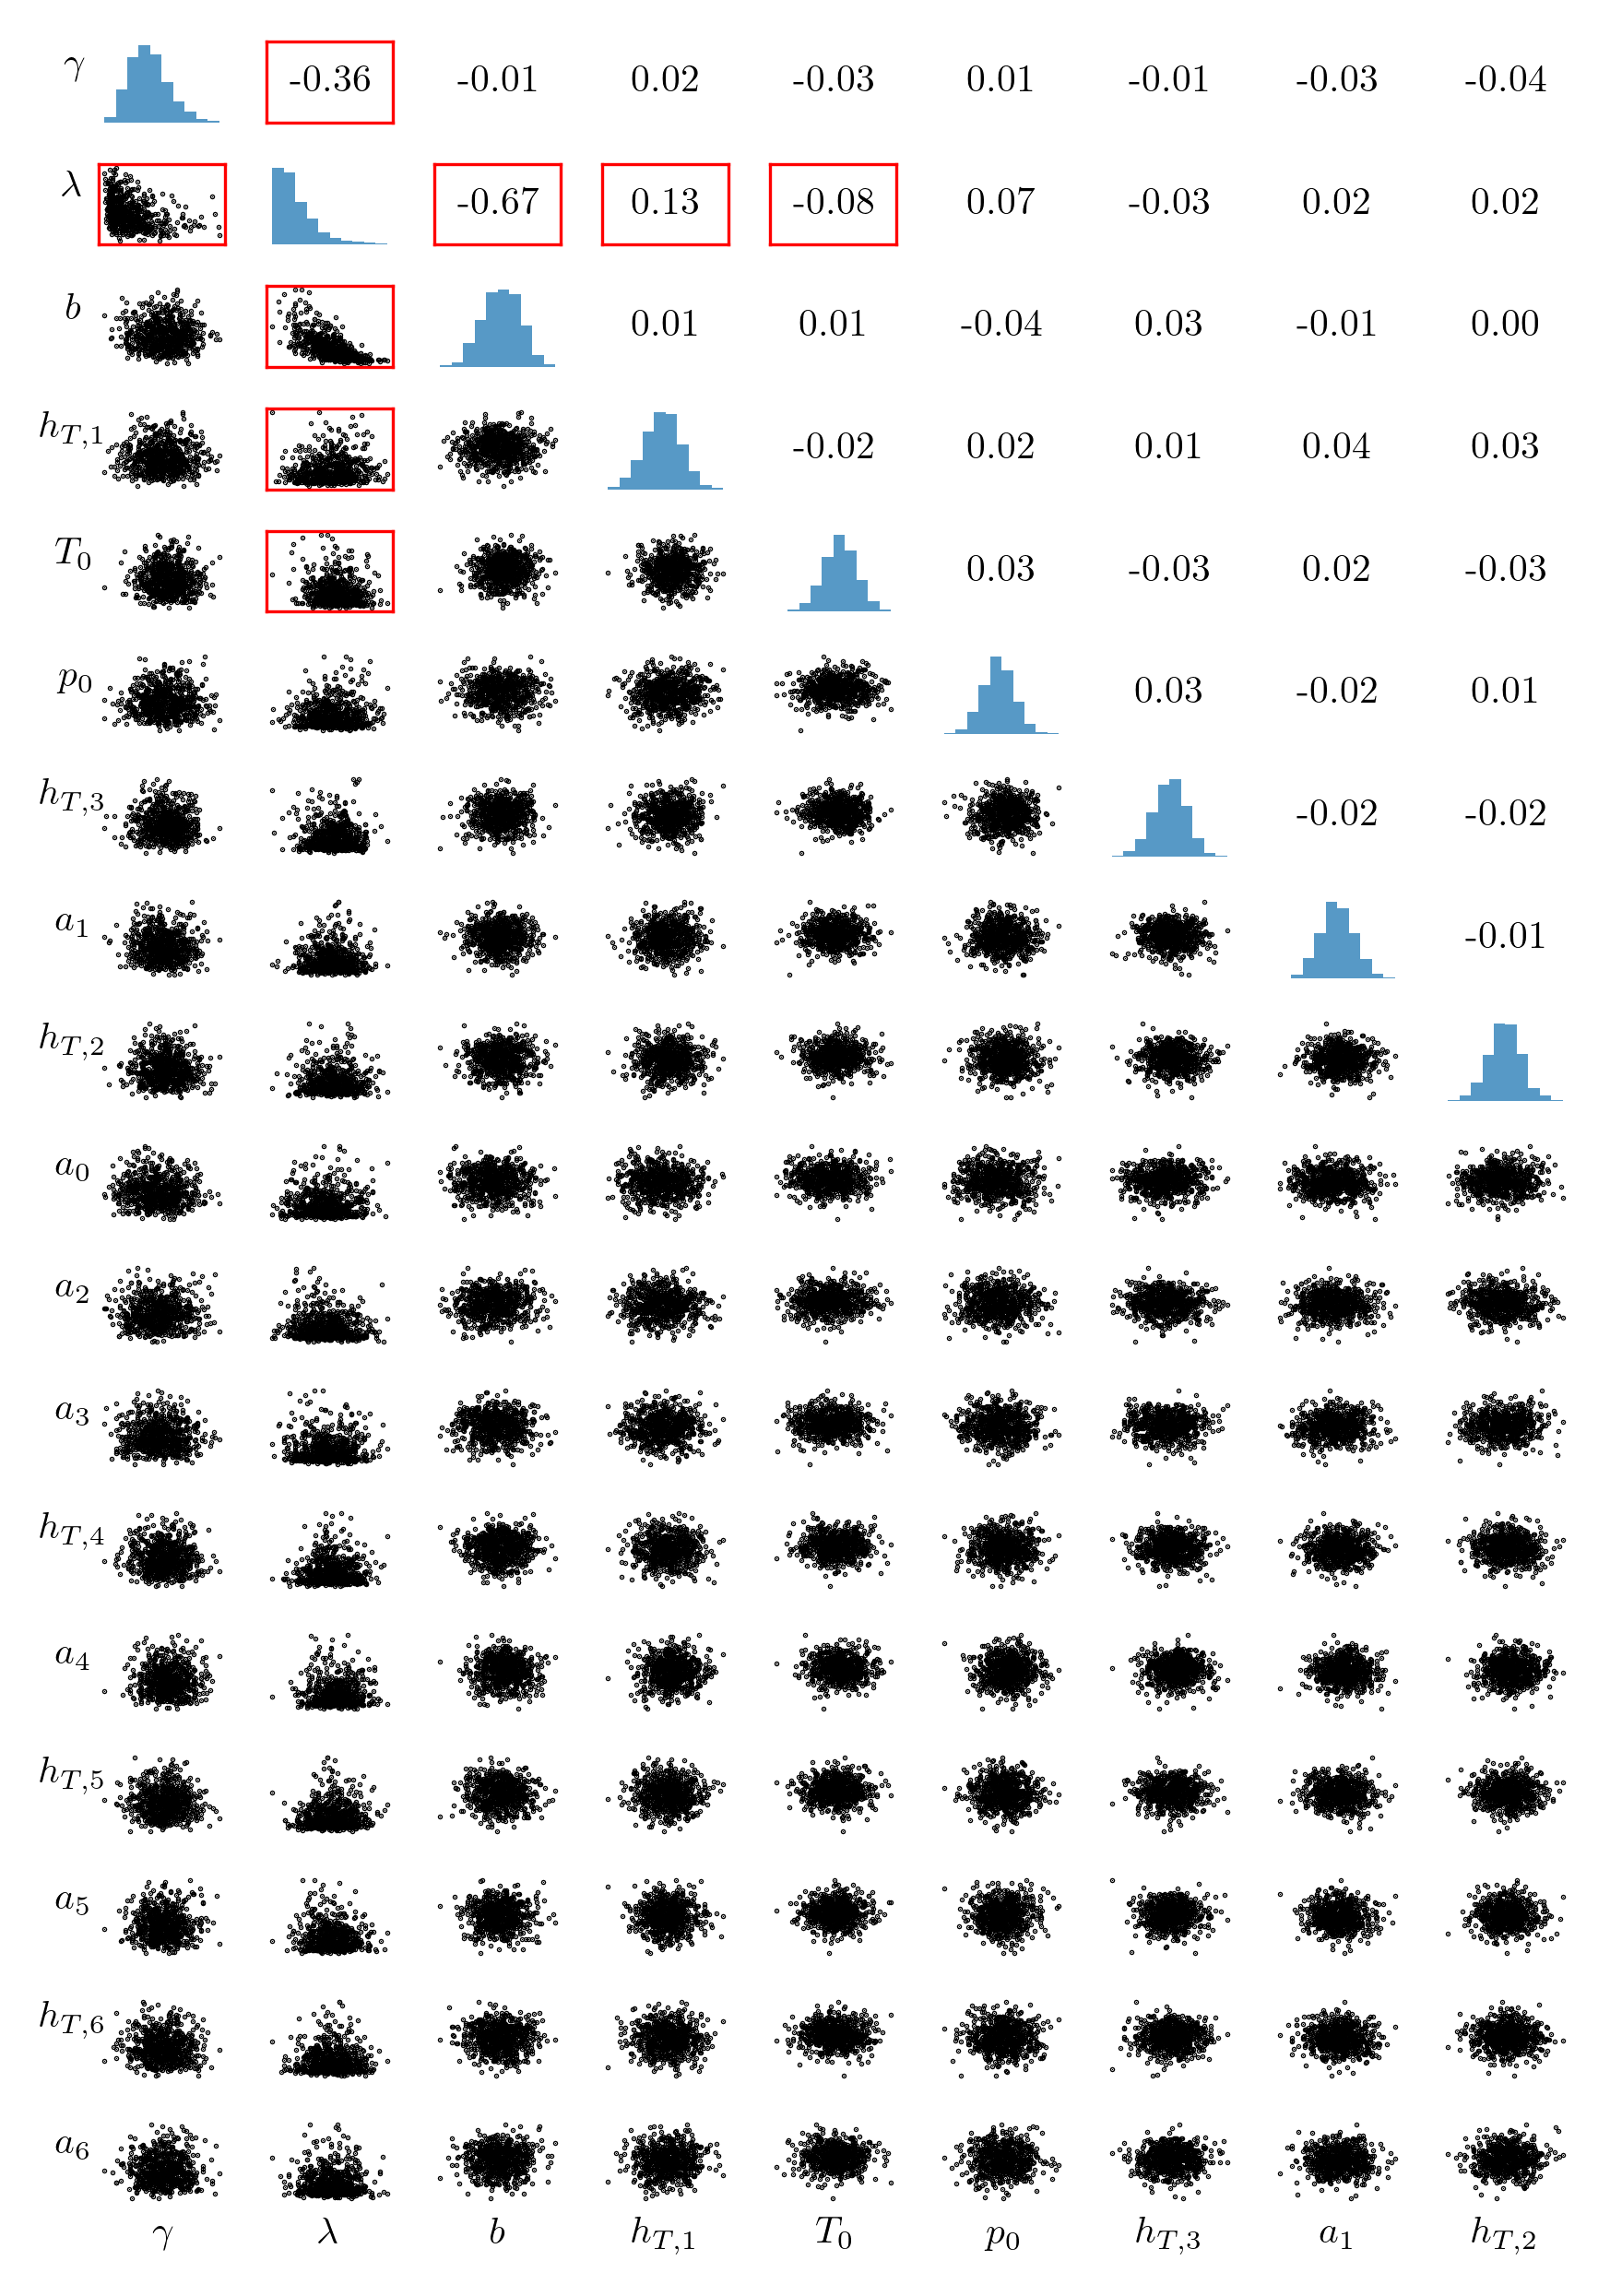
\includegraphics[]{CorrPlot.png}
	\caption[Correlation plot of samples from TT approximation]{Plot of 1000 independent samples from TT approximation of $\sqrt{\pi( \bm{\theta},\lambda,\gamma  | \bm{y})}$ via SIRT-MH scheme. We plot the Pearson correlation coefficient ranging from $-1$ to $1$ for each hyper-parameter pair.}
	\label{fig:CorrPlot}
\end{figure}
\begin{figure}% will be the right-side figure
	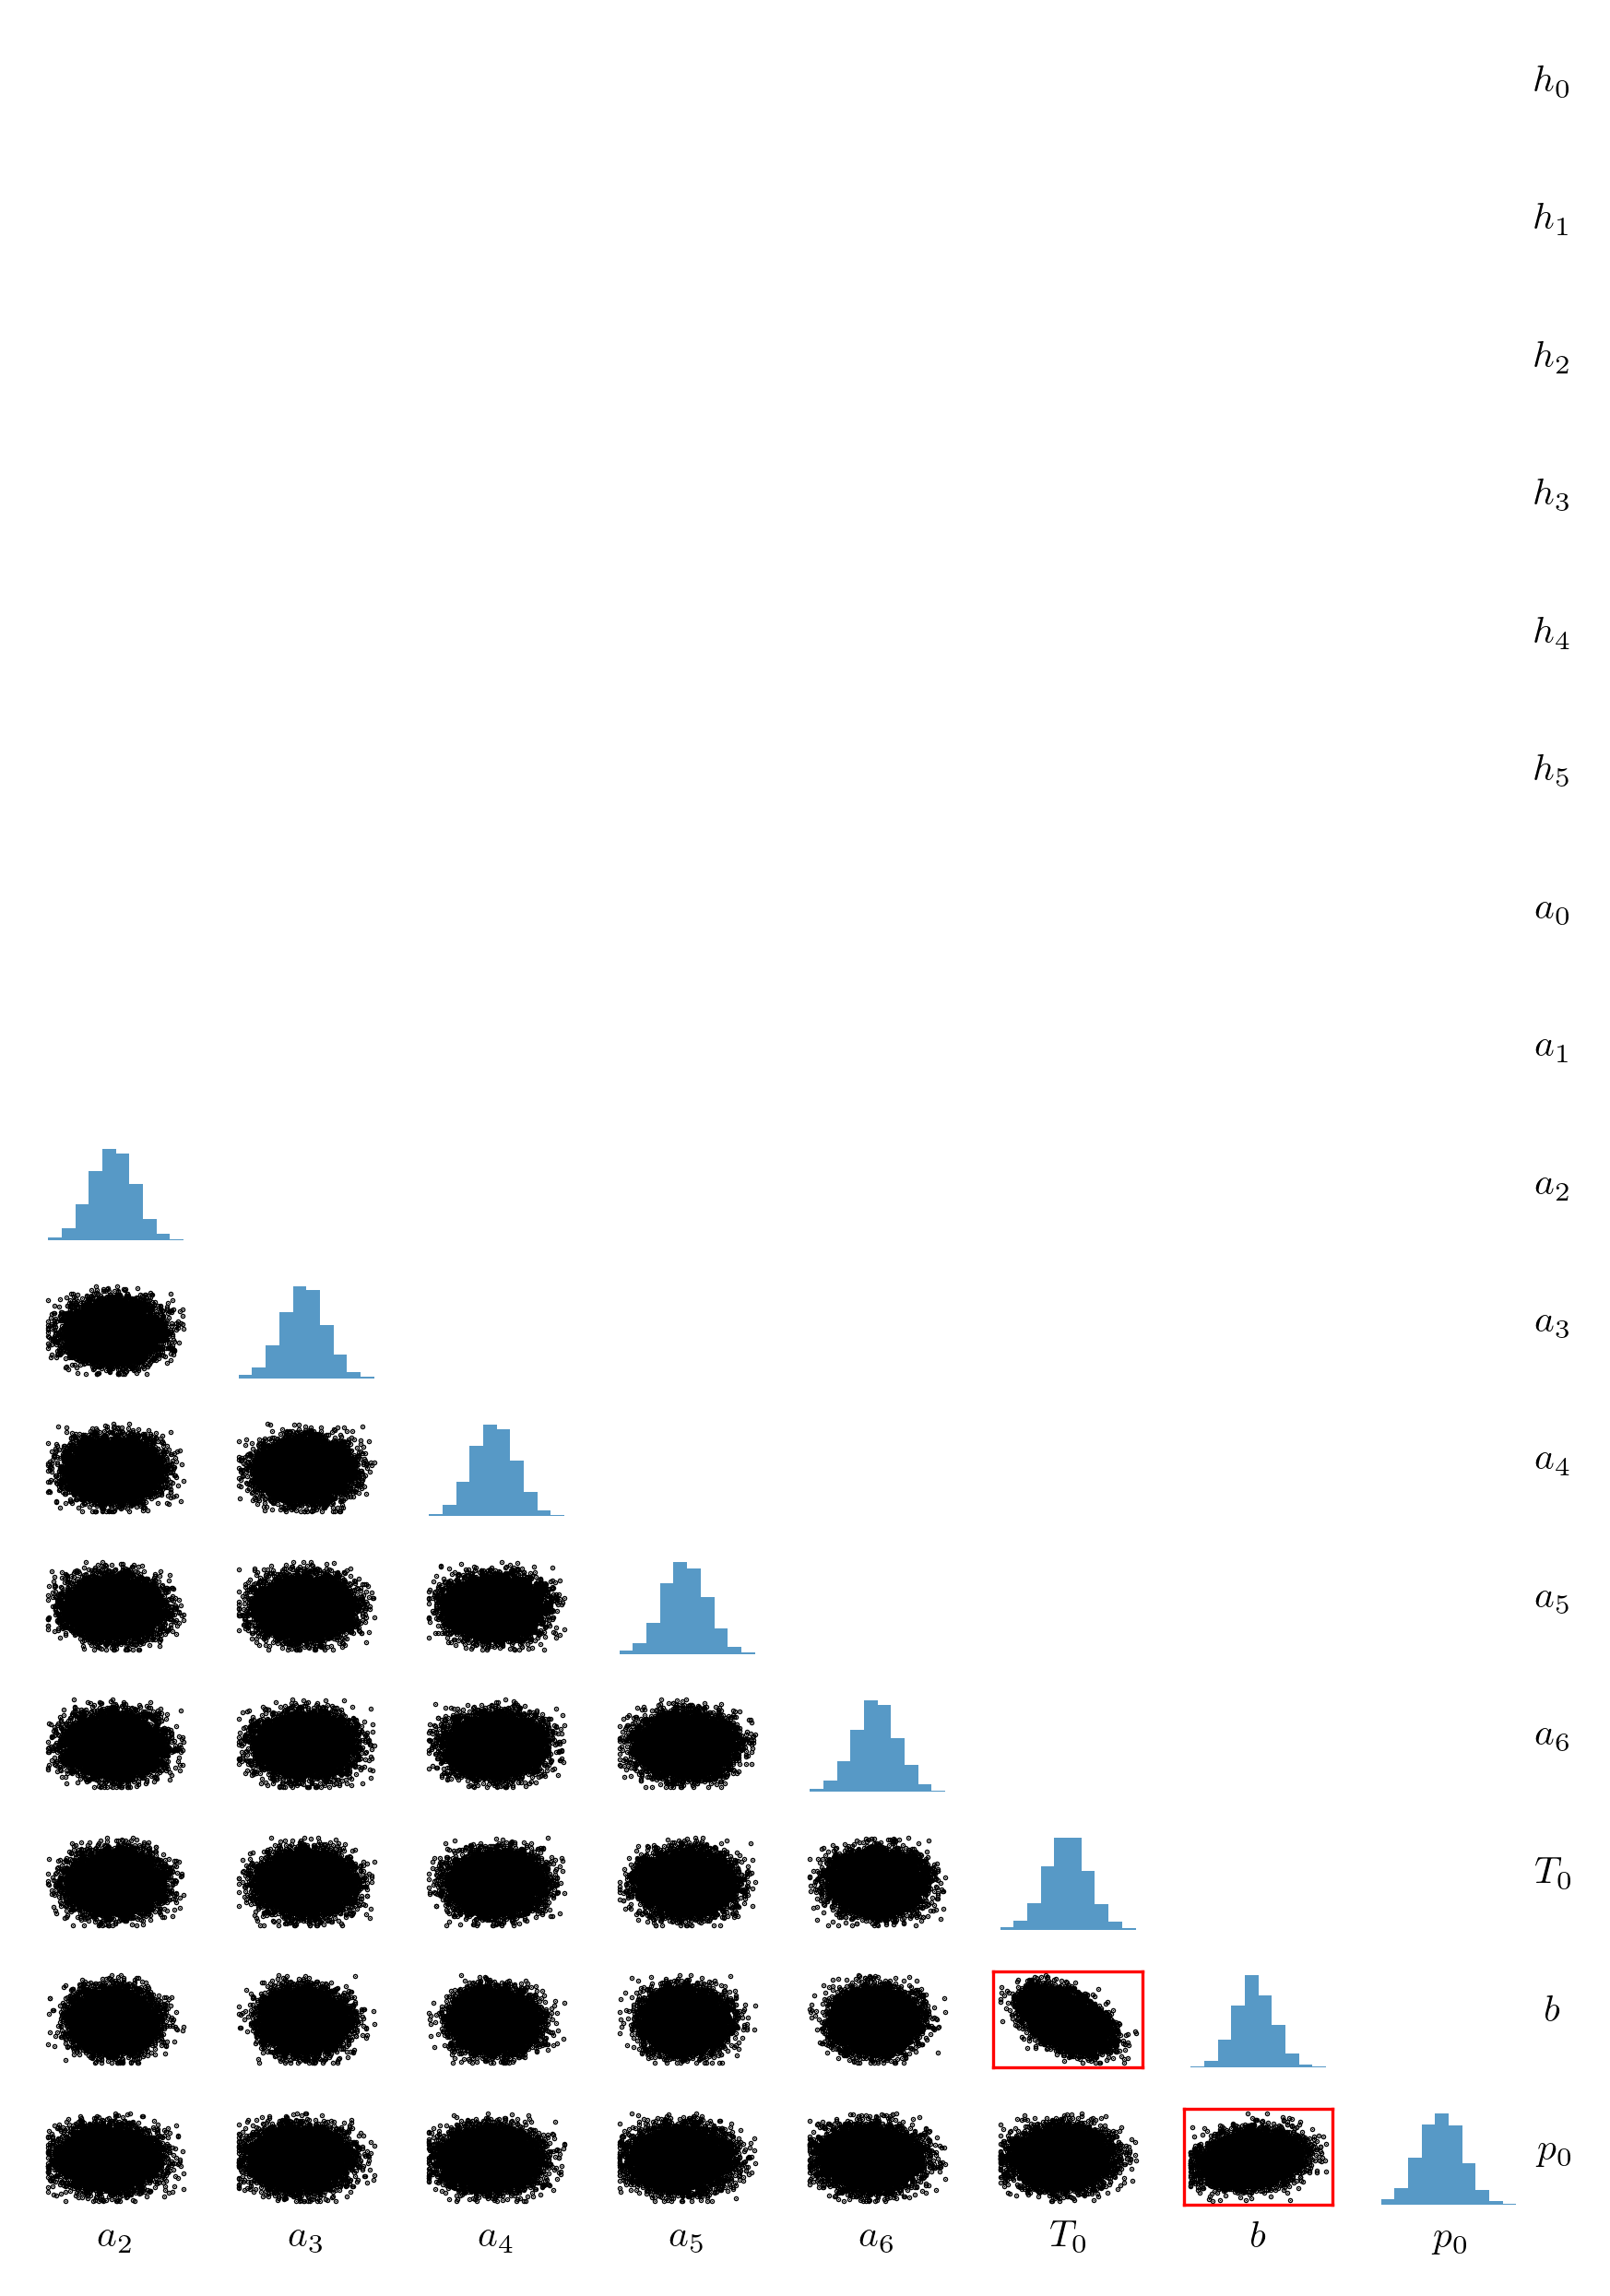
\includegraphics[]{2ndCorrPlot.png}
	\caption*{Correlation plot of samples from TT-approximation of $\sqrt{\pi(\bm{\theta},\lambda,\gamma | \bm{y})}$ via SIRT-MH scheme.}
\end{figure}



\paragraph{Find optimal rank and grid size}
The aim is to approximate $\pi( \bm{\theta},\lambda,\gamma  | \bm{y})$ with a number of function evaluations as small as possible but without losing too much accuracy.
In doing so, the number of grid points is set to $n = 150$ and different error measures for ranks $\{2,3,4,5,6,7,8,9,10,11,12,13,14,15, 20, 25, 30, 35, 50\}$ are calculated.
Then, with a fixed rank, the number of grid points \linebreak$\{10, 15, 20, 25, 30, 35, 40, 45, 50, 55, 60, 65, 70, 80, 90, 100\}$ is decreased until sufficient accuracy.

For stable and comparable results, we do five sweeps within \linebreak the~\texttt{tt.cross.rectcross.rect\_cross.cross} Python function initialised at a random TT.
The ranks between TT cores are constant.
Then $N = 1000$ independent samples  $ \{( \tilde{ \bm{\theta}},  \tilde{\lambda},  \tilde{\gamma })^{(1)} ,\dots, (\tilde{ \bm{\theta}},  \tilde{\lambda},  \tilde{\gamma })^{(N)}   \} \sim \tilde{\pi}( \bm{\theta},\lambda,\gamma  | \bm{y})$ from the TT approximation $\tilde{\pi}( \bm{\theta},\lambda,\gamma  | \bm{y})$ via the SIRT-MH scheme are drawn.
The sample mean is denoted as $\bm{\mu}_{\text{SIRT-MH}}\in \mathbb{R}^{18}$.
Further, the marginal functions from the TT approximation are used to calculate the mean $\bm{\mu}_{\text{TT}}\in \mathbb{R}^{18}$ by weighted expectations via quadrature of each hyper-parameter.
For a ground truth $N = 1000$ samples $ \{( \bm{\theta},\lambda,\gamma )^{(1)} ,\dots,( \bm{\theta},\lambda,\gamma )^{(N)}   \} \sim \pi( \bm{\theta},\lambda,\gamma  | \bm{y})$
are obatined via t-walk and the sample mean $ \bm{\mu}_{\text{t-walk}}  \in \mathbb{R}^{18}$ acts as a ground thruth.
The true marginal posterior is denoted as $ \pi( \bm{\theta},\lambda,\gamma  | \bm{y})$.

Plotted in Fig.~\ref{fig:FindRankGrid}, for each tested TT approximation, the following error measures are calculated:
\begin{itemize}
	\item[{
\includegraphics[height=0.65\baselineskip]{SIRTMH.png}}] The \textbf{relative expectation Errorr (SIRT-MH)}
	\begin{align*} 
		\frac{\lVert\bm{\mu}_{\text{SIRT-MH}} - \bm{\mu}_{\text{t-walk}} \rVert_{L^2}}{  \lVert \bm{\mu}_{\text{t-walk}} \rVert_{L^2} } \, .
	\end{align*}
	\item[{
\includegraphics[height=0.65\baselineskip]{QUAD.png}}] The \textbf{relative expectation Error (quadrature)}
	\begin{align*} 
		\frac{\lVert\bm{\mu}_{\text{TT}} - \bm{\mu}_{\text{t-walk}} \rVert_{L^2} }{ \lVert \bm{\mu}_{\text{t-walk}} \rVert_{L^2} } \, .
	\end{align*}
	\item[{
\includegraphics[height=0.65\baselineskip]{RMS.png}}] The \textbf{relative RMS Error} 
	\begin{align*} 
		\frac{\lVert \tilde{\pi}(\tilde{ \bm{\theta}},  \tilde{\lambda},  \tilde{\gamma})  - \pi(\tilde{ \bm{\theta}},  \tilde{\lambda},  \tilde{\gamma}) \rVert_{L^2} }{ \lVert \pi(\tilde{ \bm{\theta}},  \tilde{\lambda},  \tilde{\gamma})  \rVert_{L^2} } \, .
	\end{align*}
	\item[{
\includegraphics[height=0.65\baselineskip]{W1.png}}] The \textbf{1-Wasserstein Distance}
	\begin{align*} 
		W_1(\pi,\tilde{\pi}) = 	\underset{\nu \in \Pi(\pi,\tilde{\pi}) }{\text{min}} \sum^N_{i,j =1}  \nu_{ij} \lVert \text{vec}\big(( \bm{\theta},\lambda,\gamma ) ^{(i)} \big)-  \text{vec}\big( (\tilde{ \bm{\theta}},  \tilde{\lambda},  \tilde{\gamma})^{(j)}\big) \rVert_{L^2} \, .
	\end{align*}
\end{itemize} 
The 1-Wasserstein distance as in Eq.~\ref{eq:applWasser} is calculated between 1000 independent SIRT-MH samples from the TT approximation $\tilde{\pi}( \bm{\theta},\lambda,\gamma  | \bm{y})$ weighted by their approximated values and 1000 independent t-walk samples from the true marginal posterior weighted by $\pi( \bm{\theta},\lambda,\gamma  | \bm{y})$.
Here $\text{vec}( \bm{\theta},\lambda,\gamma )$ denotes the vector of hyper-parameters $\big( \bm{\theta}^T,\lambda^T,\gamma^T \big)^T \in \mathbb{R}^{18}$ and $\nu_{ij} \coloneqq  \tilde{\pi}\big( (\tilde{ \bm{\theta}},  \tilde{\lambda},  \tilde{\gamma})^{(j)}   | \bm{y}\big)  \pi\big( (\bm{\theta},\lambda,\gamma )^{(i)}  | \bm{y}\big) $.
As in~\cite{feydy2020OT} we normalise over the samples so that $\sum \pi\big( (\bm{\theta},\lambda,\gamma )^{(i)}  | \bm{y}\big)  = 1$ and $\sum \tilde{\pi}\big( (\tilde{ \bm{\theta}},  \tilde{\lambda},  \tilde{\gamma})^{(j)}   | \bm{y}\big) = 1$.
We use the Python function \texttt{SamplesLoss("sinkhorn", p$=1$, blur$=0.05$, scaling=0.8)} with default settings from the Python package \texttt{geomloss}~\cite{Wassersteinaccess} to obtain $W_1$.
This function provides the unbiased Sinkhorn divergence which converges towards the Wasserstein distance and can be understood as the generalised Quicksort algorithm~\cite{feydy2020OT}.
Here p$ = 1$ defines the distance measure $\lVert \cdot \rVert_{L^2}$.
The blur parameter is an entropic penalty and the scaling parameter specifies the trade-off between speed (scaling $< 0.4$) and accuracy (scaling $>0.9$)~\cite{Wassersteinaccess}.


\begin{figure}[ht!]
	\centering
	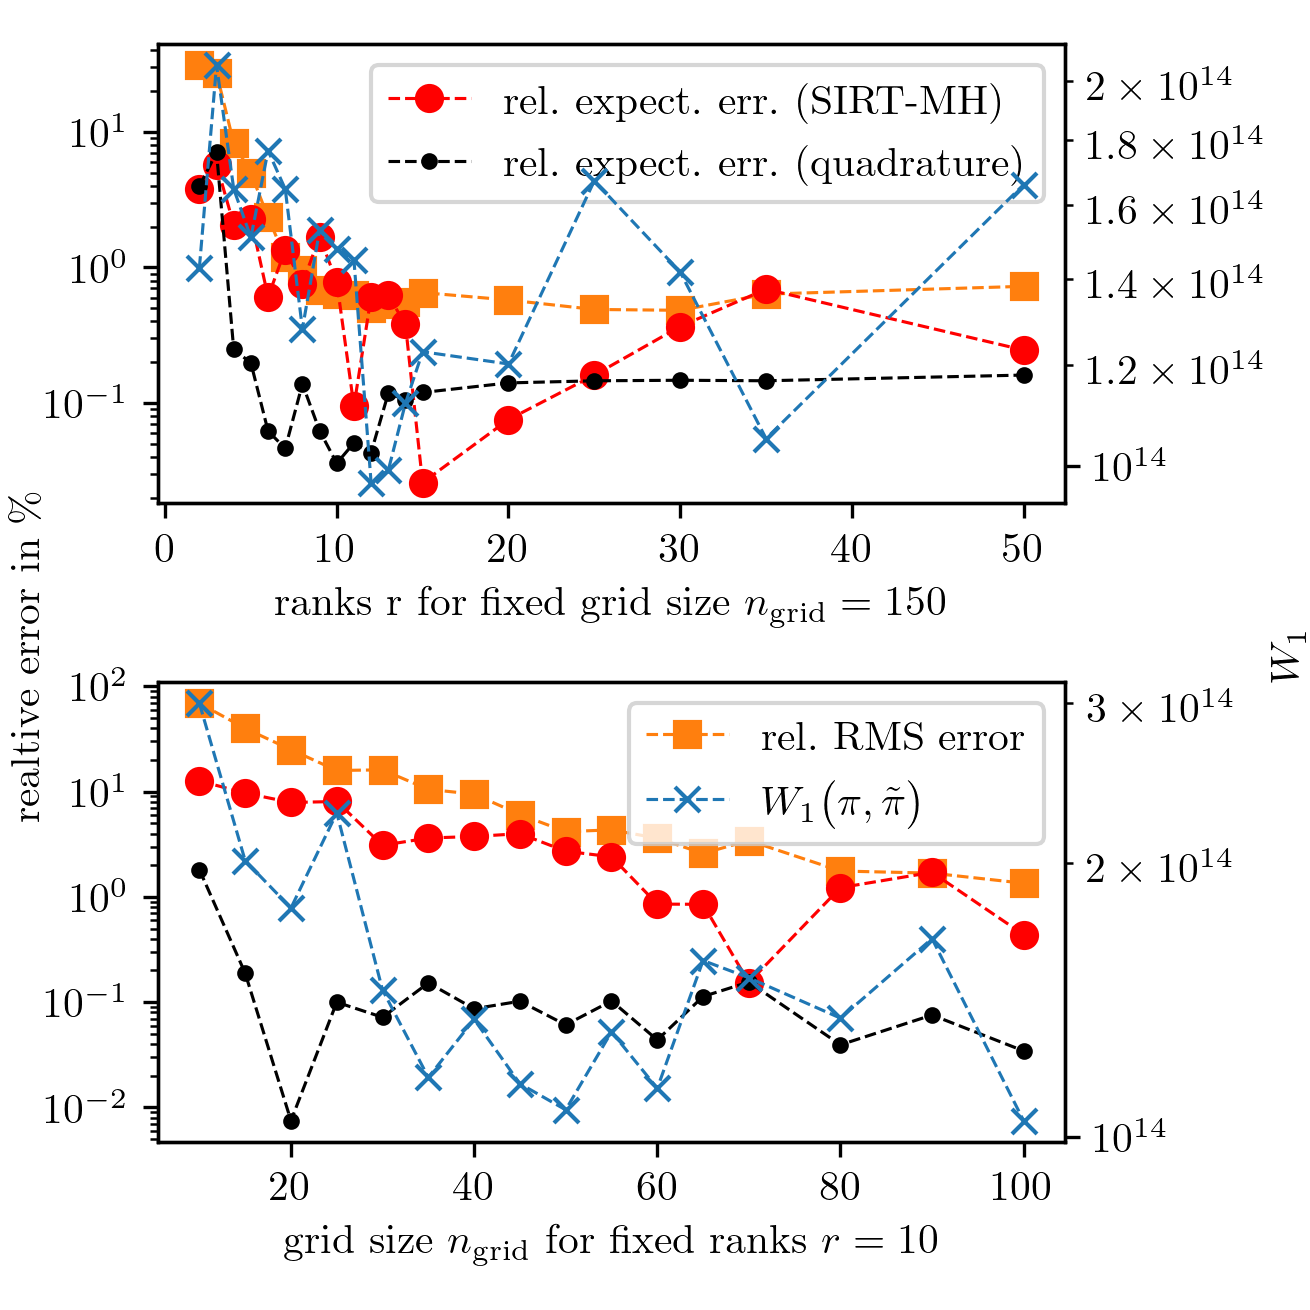
\includegraphics[]{findGridRank.png}
	\caption[Optimal rank and number of grid points for TT approximation.]{Given a TT approximation of $\sqrt{\pi( \bm{\theta},\lambda,\gamma  | \bm{y}) }$, the relative RMS error (orange squares) between approximated values at sample points provided by the SIRT-MH and true function values are calculated. The relative RMS error between the sample means provided by the t-walk and mean values for the hyper-parameters from the TT approximation is plotted (black dots). The mean values for the hyper-parameters are computed via quadrature, where the marginal functions from the TT approximation act as quadrature weights. Additionally, the relative RMS error between the sample-based mean from the SIRT-MH and the sample-based mean from the t-walk (red circles) is plotted.  The 1-Wasserstein distance (blue cross) is calculated between SIRT-MH samples and t-walk samples weighted by their repective approxiamted or true function value.}
	\label{fig:FindRankGrid}
\end{figure}
 
In Fig.~\ref{fig:FindRankGrid} we observe that a rank $r = 10$ is sufficient because the error measures are relatively stable for $r\geq10$.
For a grid size $n \geq 30$ the relative differences between $\bm{\mu}_{\text{TT}}$ and $\bm{\mu}_{\text{t-walk}}$ (red circles in Fig.~\ref{fig:FindRankGrid}) and the RMS errors at the 1000 independent SIRT-MH samples (orange squares in Fig.~\ref{fig:FindRankGrid}) are around $ 10\%$ and considered good enough.
For an increasing number of grid points the interpolation of function values between grid points is more accurate and the sample-based relative errors decrease.
This is because the chosen linear interpolation (see Eq.~\ref{eq:LinPol}) is a rather rudimentary choice.
The quadrature-based relative expectation error (black dots in Fig.~\ref{fig:FindRankGrid}) is almost constant for ranks $ \gtrsim 7$ and grid sizes $ > 20$.
Since the hyper-parameters have different length scales, we are only interested in the trend of the sample-based 1-Wasserstein distance (blue crosses in Fig.~\ref{fig:FindRankGrid}).
The 1-Wasserstein distance is quite fluctuant but decreases with increasing ranks and stays within a similar range for grid sizes $n \geq 30$.


\begin{figure}[ht!]
	\centering
	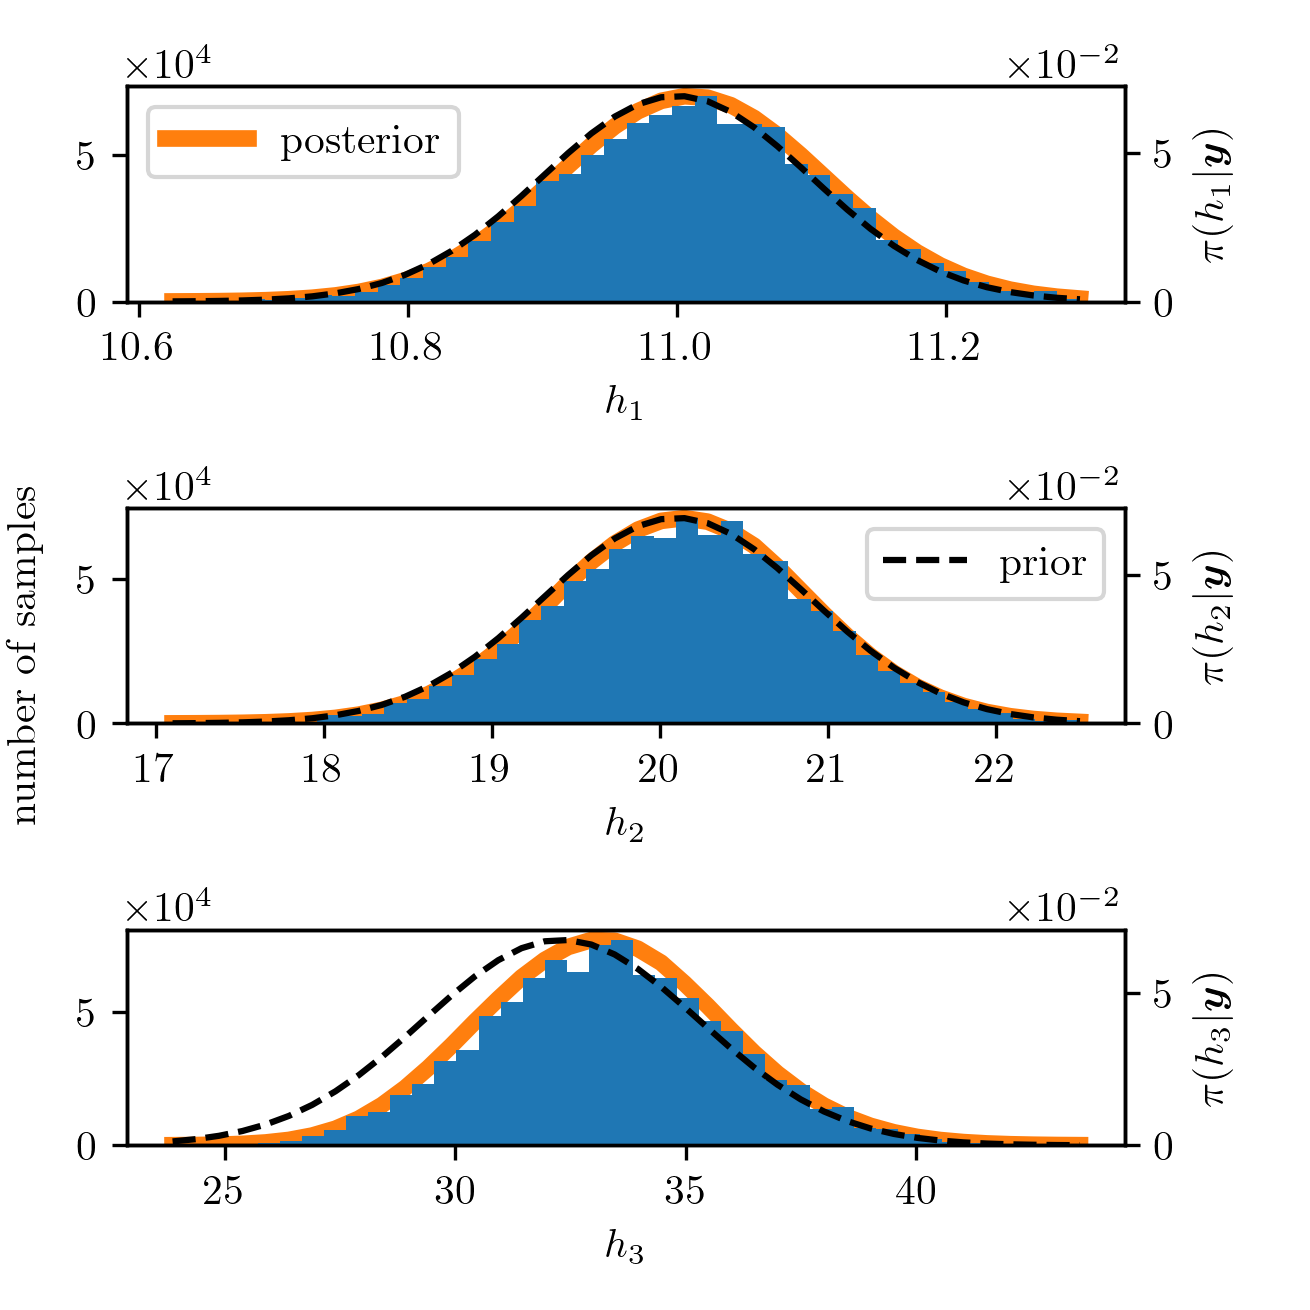
\includegraphics{PHdPTPost0.png}
	\caption[Histograms and TT approximation of posterior distribution as well as hyper-prior distribution.]{TT approximation of the marginal posterior in orange and the samples from the t-walk as a histogram, as well as the prior distribution with a dotted line.}
	\label{fig:PostHistTT0}
\end{figure}
\begin{figure}[ht!]
	\centering
	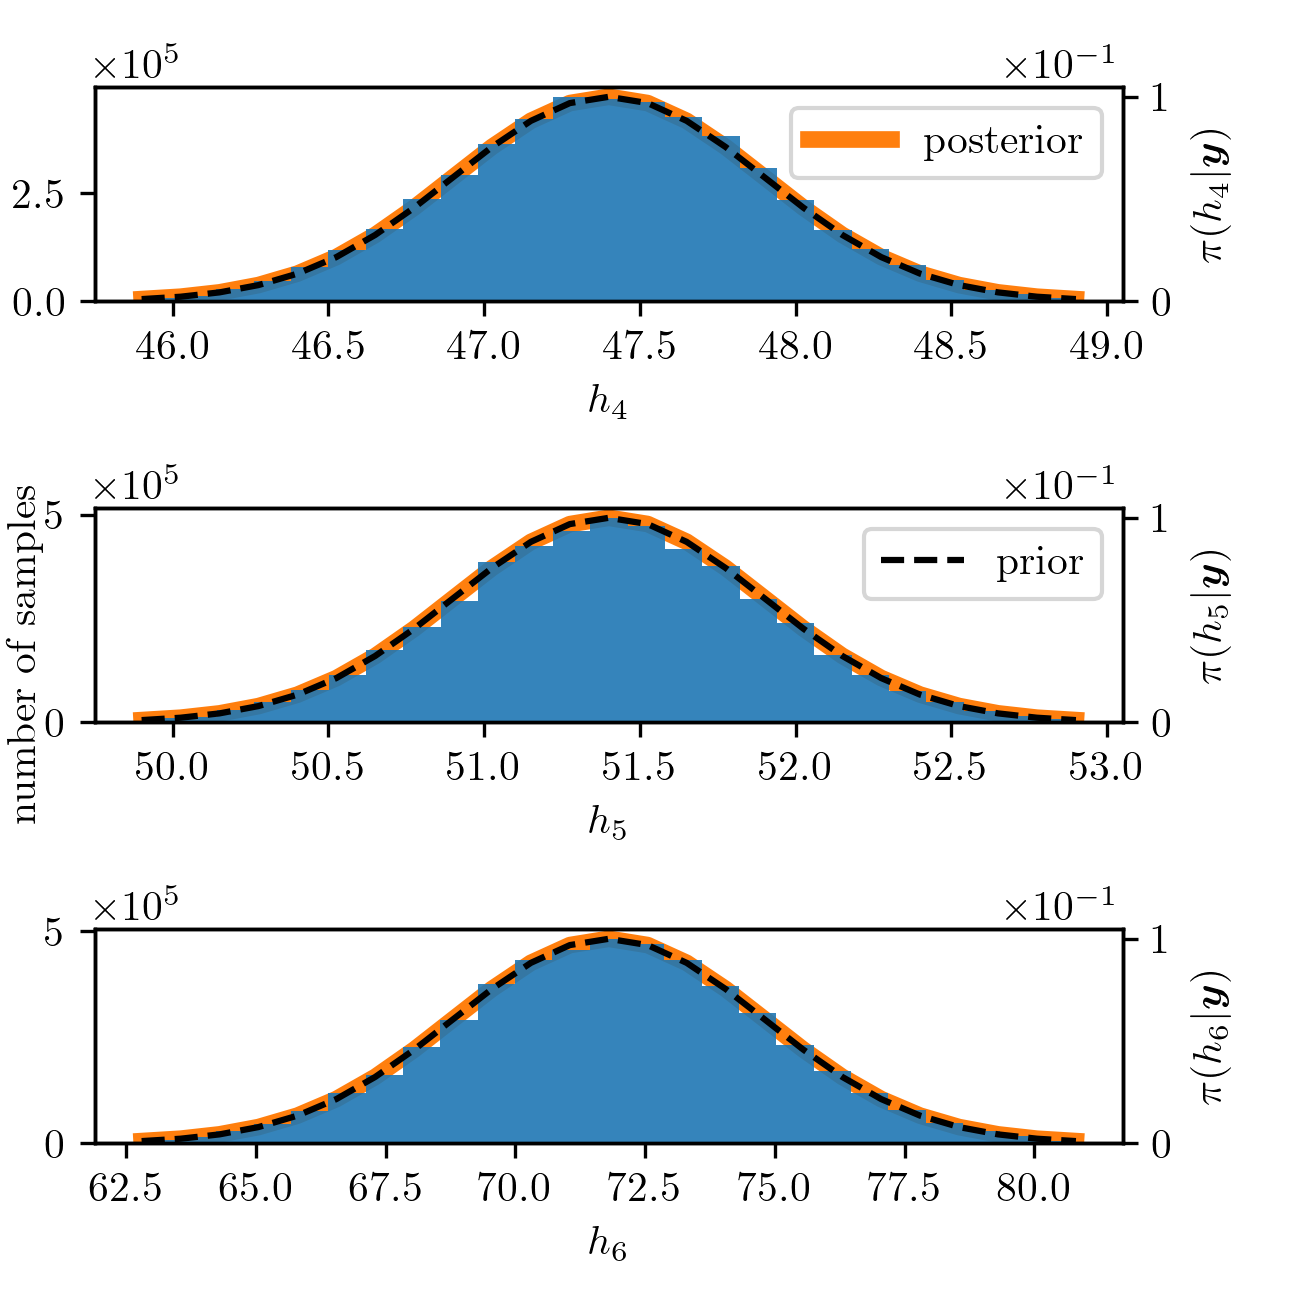
\includegraphics{PHdPTPost1.png}
	\caption[Histograms and TT approximation of posterior distribution as well as hyper-prior distribution.]{TT approximation of the marginal posterior in orange and the samples from the t-walk as a histogram, as well as the prior distribution with a dotted line.}
	\label{fig:PostHistTT1}
\end{figure}
\begin{figure}[ht!]
	\centering
	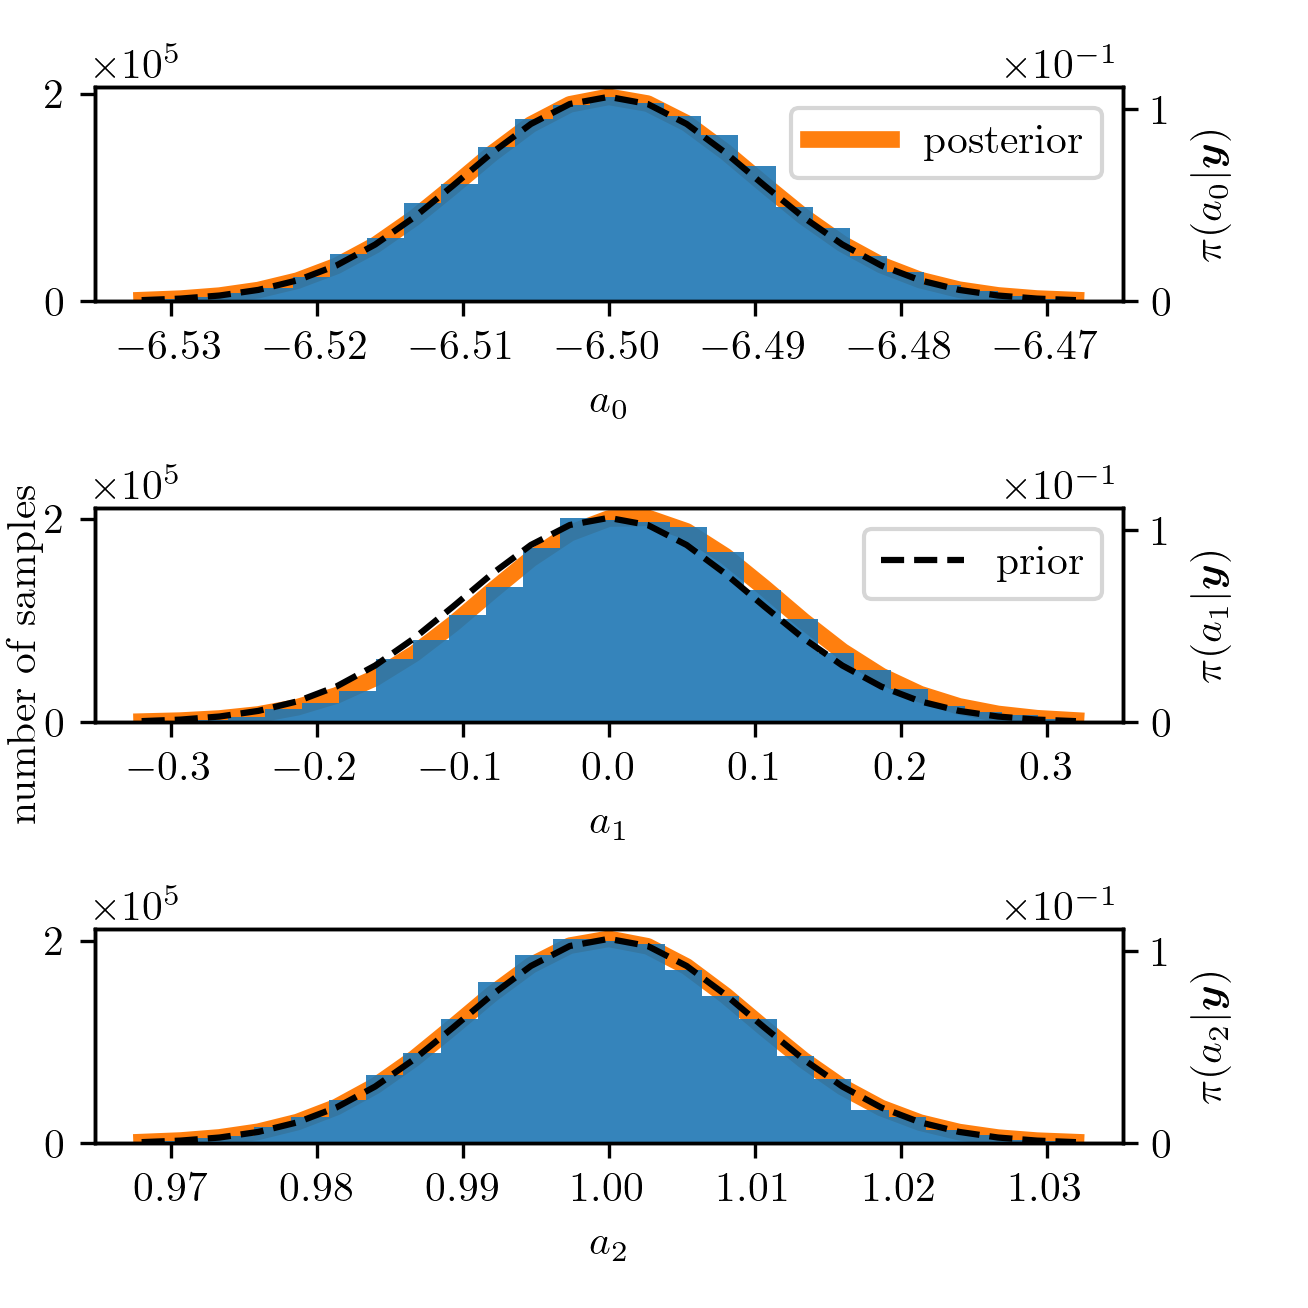
\includegraphics{PHdPTPost2.png}
	\caption[Histograms and TT approximation of posterior distribution as well as hyper-prior distribution.]{TT approximation of the marginal posterior in orange and the samples from the t-walk as a histogram, as well as the prior distribution with a dotted line.}
	\label{fig:PostHistTT2}
\end{figure}
\begin{figure}[ht!]
	\centering
	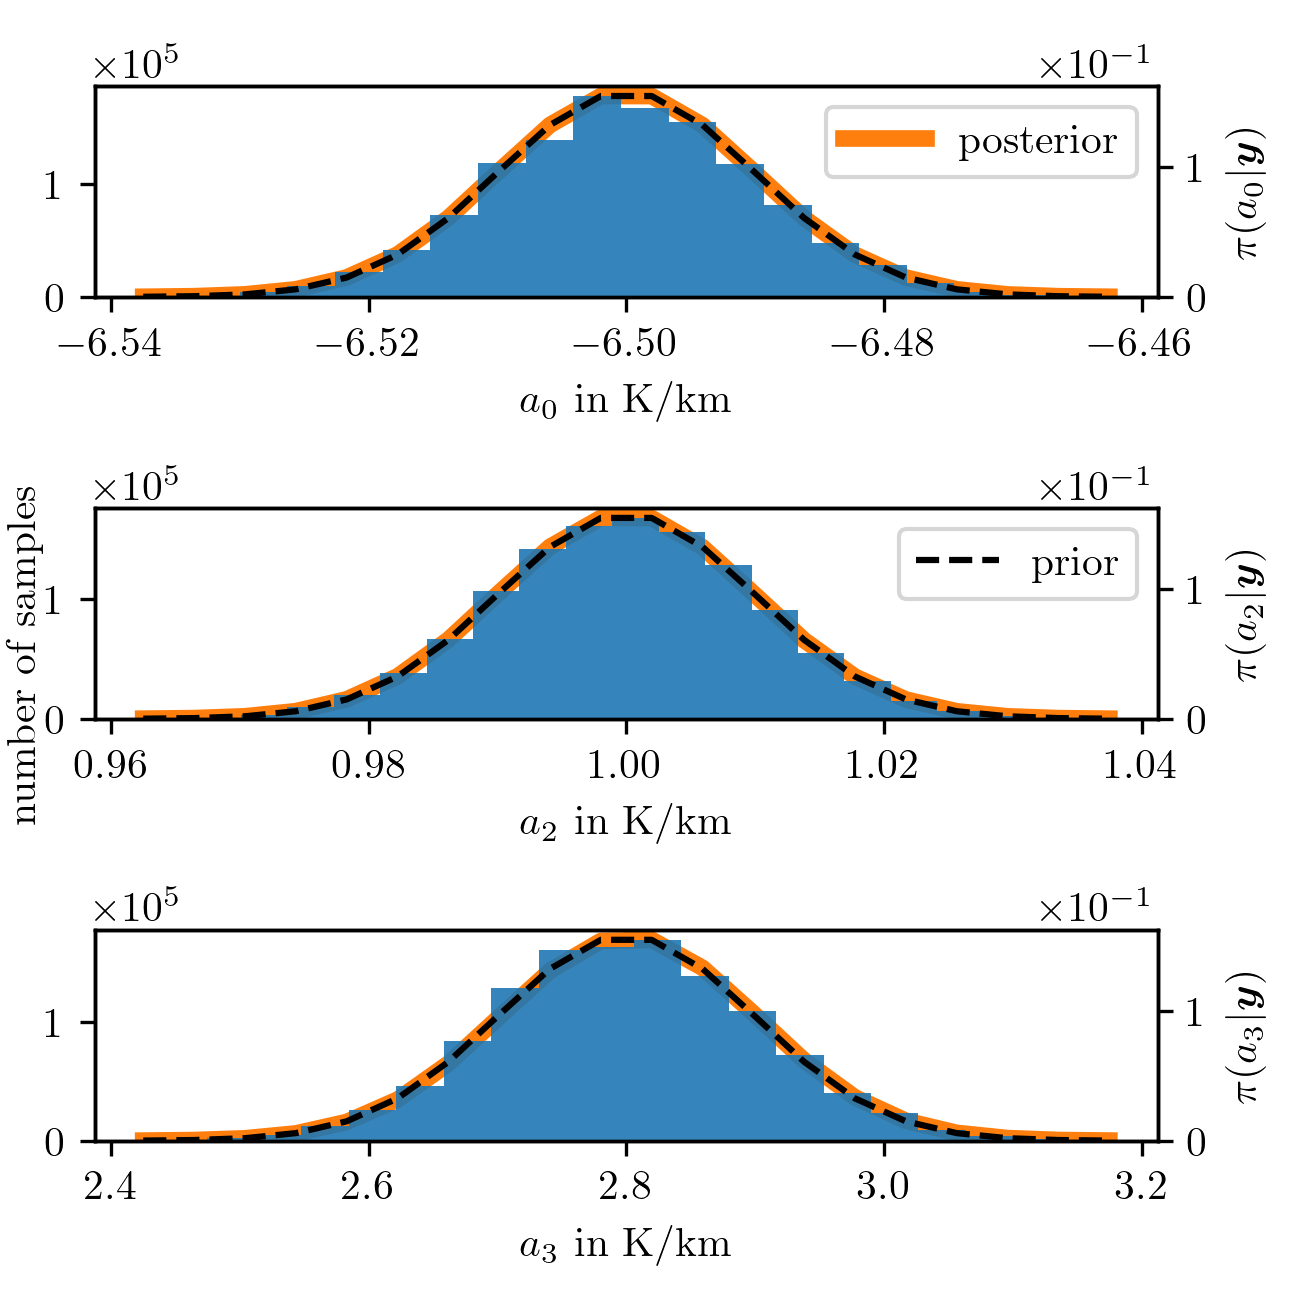
\includegraphics{PHdPTPost3.png}
	\caption[Histograms and TT approximation of posterior distribution as well as hyper-prior distribution.]{TT approximation of the marginal posterior in orange and the samples from the t-walk as a histogram, as well as the prior distribution with a dotted line.}
	\label{fig:PostHistTT3}
\end{figure}
\begin{figure}[ht!]
	\centering
	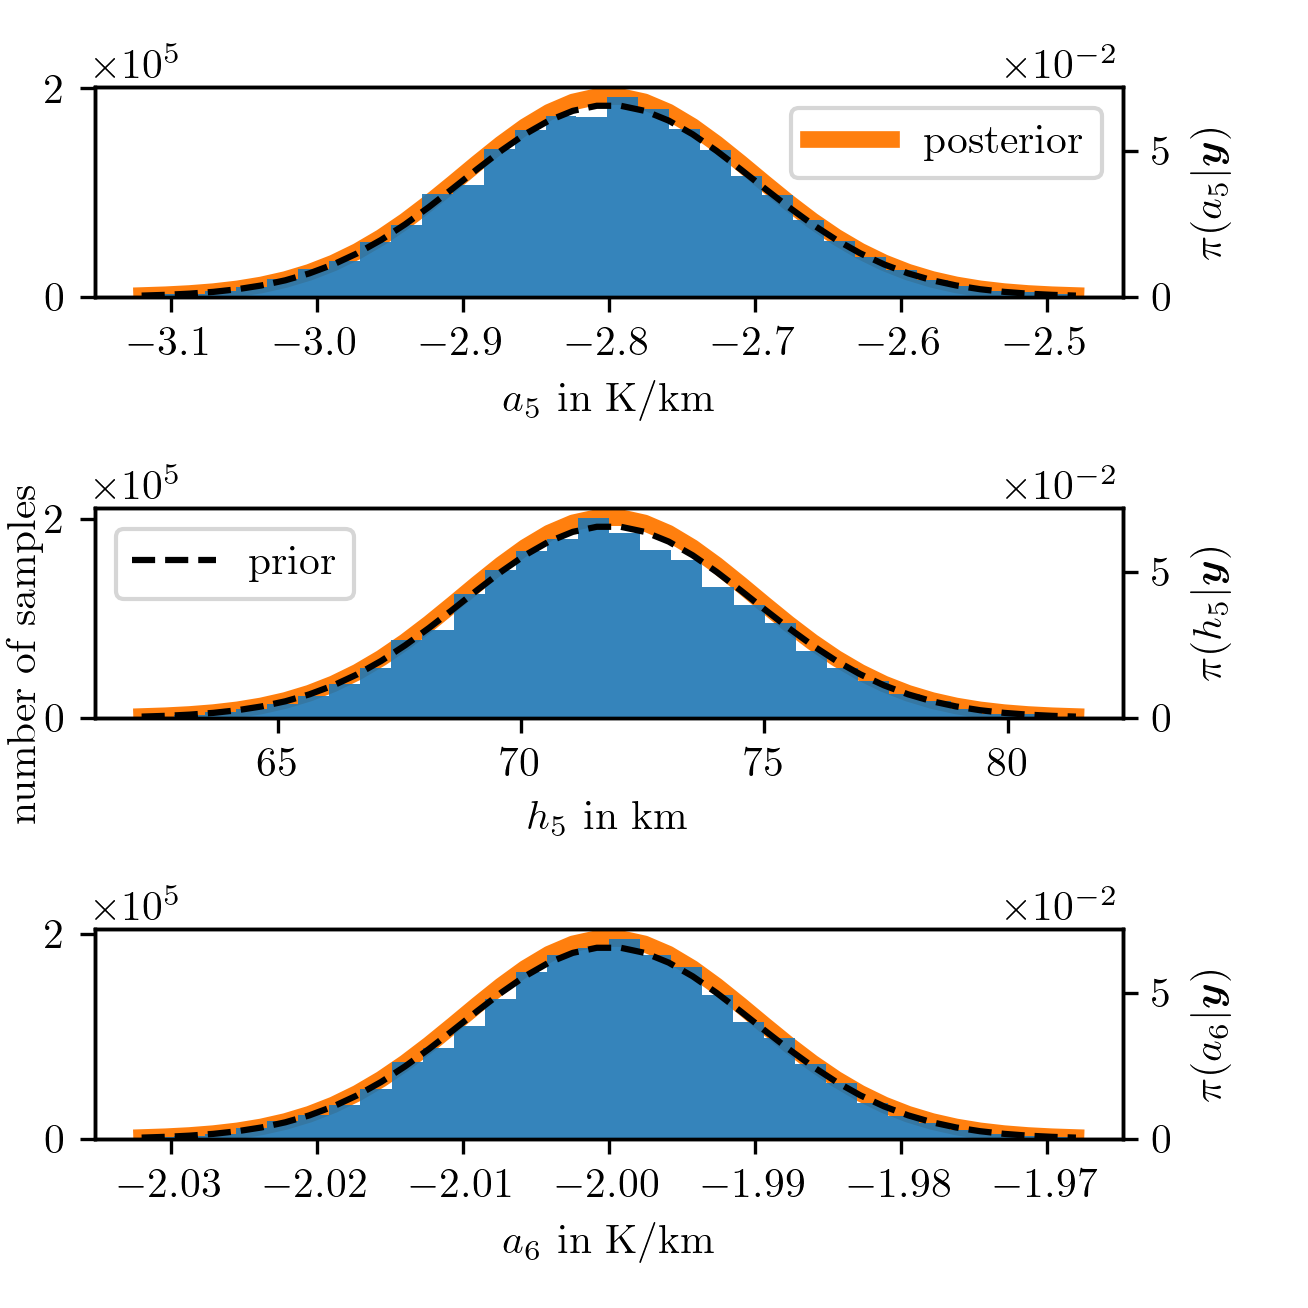
\includegraphics{PHdPTPost4.png}
	\caption[Histograms and TT approximation of posterior distribution as well as hyper-prior distribution.]{TT approximation of the marginal posterior in orange and the samples from the t-walk as a histogram, as well as the prior distribution with a dotted line.}
	\label{fig:PostHistTT4}
\end{figure}
\begin{figure}[ht!]
	\centering
	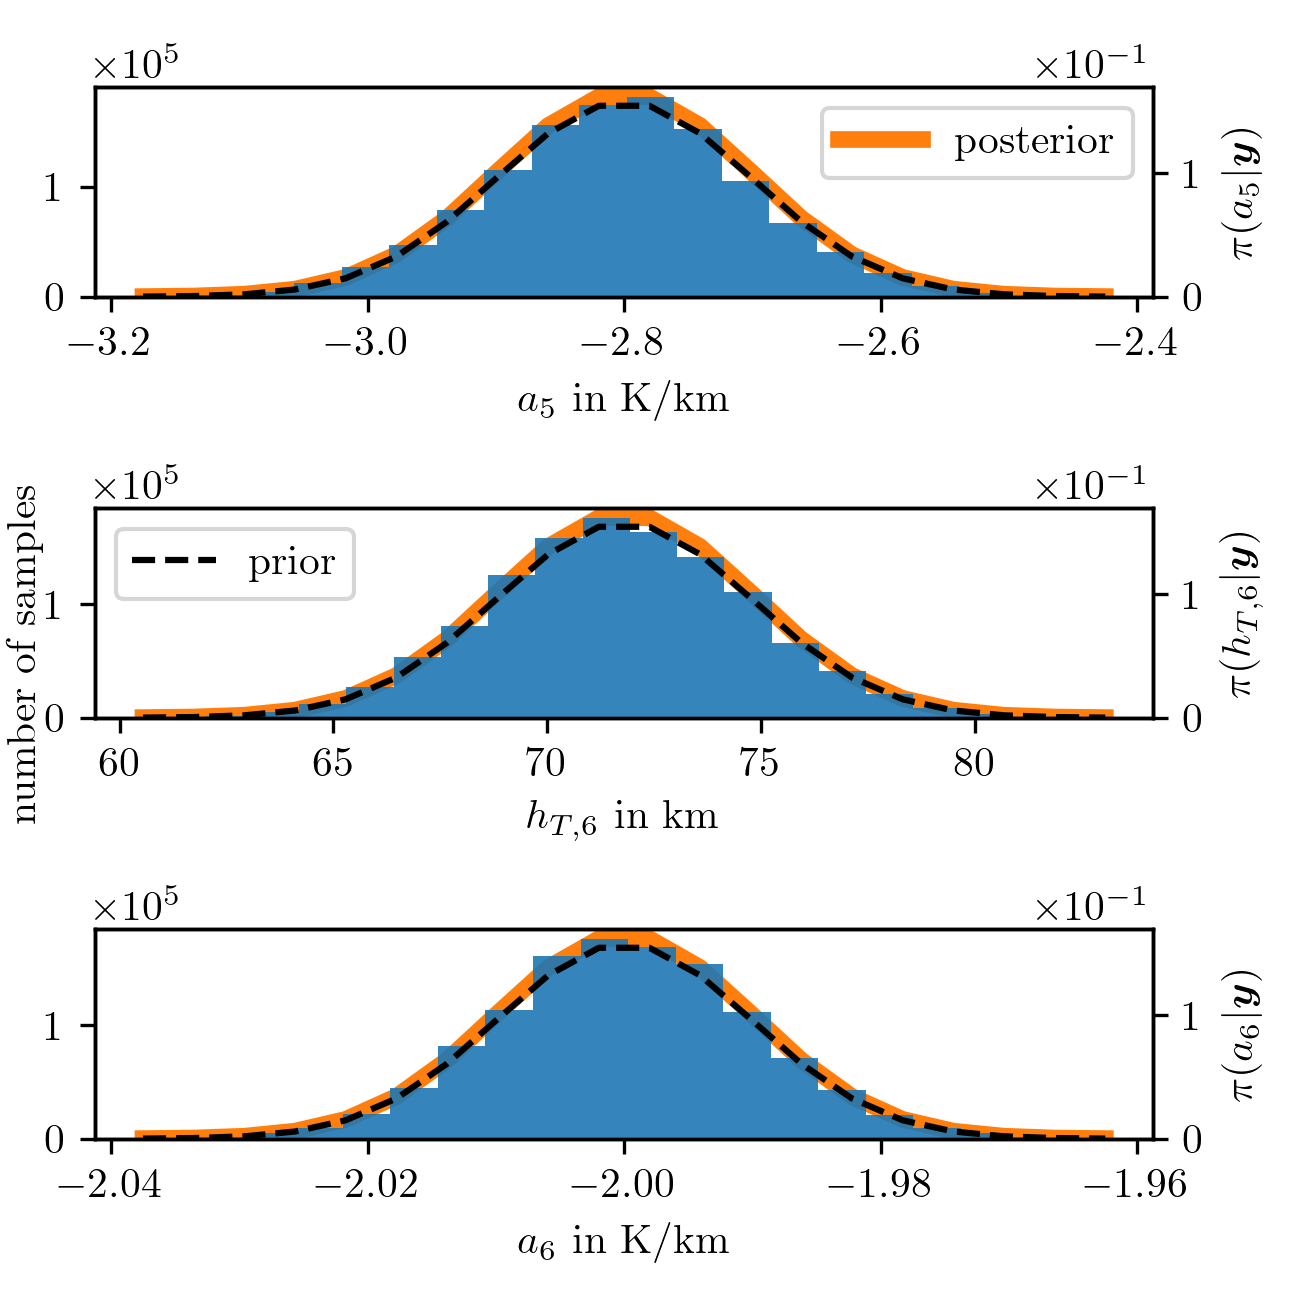
\includegraphics{PHdPTPost5.png}
	\caption[Histograms and TT approximation of posterior distribution as well as hyper-prior distribution.]{TT approximation of the marginal posterior in orange and the samples from the t-walk as a histogram, as well as the prior distribution with a dotted line.}
	\label{fig:PostHistTT5}
\end{figure}

Based on these results the grid size is set to $n = 30$.
Next, we define ranks $r =[ 1,  10,  10, 10, 10, 10, 5, 3, 3, 3, 3, 3, 3 , 3, 3, 3, 3, 3, 1]$ between TT cores, with a maximum rank of $10$.
This harvests the correlation structure of $\pi(\bm{\theta},\lambda,\gamma  | \bm{y})$ and decreases the number of function evaluations even further.
One sweep in the\linebreak \texttt{tt.cross.rectcross.rect\_cross.cross} initialised at a previously calculated approximation reduces the computation time to $\approx 10$s and the number of function evaluations to 34080.
For the samples drawn via the SIRT-MH scheme, the average IACT (provided by twice the value of~\cite{wolff2004monte, drikHesse}) is $\approx 1.2 \pm 0.2$.
This means that once the TT approximation is available two function evaluations per independent sample are needed.
To draw 1000 independent samples, including generating a TT approximation, takes $\approx30$s, and we report a relative RMS error of $\approx 12 \%$ evaluated over those 1000 independent samples.
The relative RMS error over 1000 randomly chosen grid points is $\approx 1\%$ indicating that the linear interpolation causes most of the approximation error.
The marginals for each hyper-parameter are plotted in Fig.~\ref{fig:PostHistTT0} to Fig.~\ref{fig:PostHistTT5}.
We observe that, besides $\lambda$ and $\gamma$, only the marginal posterior of the $b$ hyper-parameter is seriously affected by the data and has significantly changed compared to the hyper-prior distribution.
\clearpage

\subsubsection{Posterior pressure and temperature}
Posterior pressure and temperature profiles are directly obtained by hyper-parameter samples from the marginal posterior $\pi(\bm{\theta},\lambda,\gamma  | \bm{y})$ and then calculated according to their respective function (see Eq.~\ref{eq:tempFunc} and Eq.~\ref{eq:pressFunc}).
The obtained pressure and temperature posterior profiles are plotted in Fig.~\ref{fig:PressPost} and Fig.~\ref{fig:TempPost}.
The posterior temperature profiles look (as expected) similar to the prior temperature profiles, whereas the pressure profile has slightly larger values compared to the ground truth.
This is because the hyper-parameter $b$ is smaller than its ground truth value (see Fig.~\ref{fig:PostHistTT0}), resulting in the posterior pressure profiles that do not exponentially decrease as fast as the ground truth pressure profile.

\begin{figure}[ht!]
	\centering
	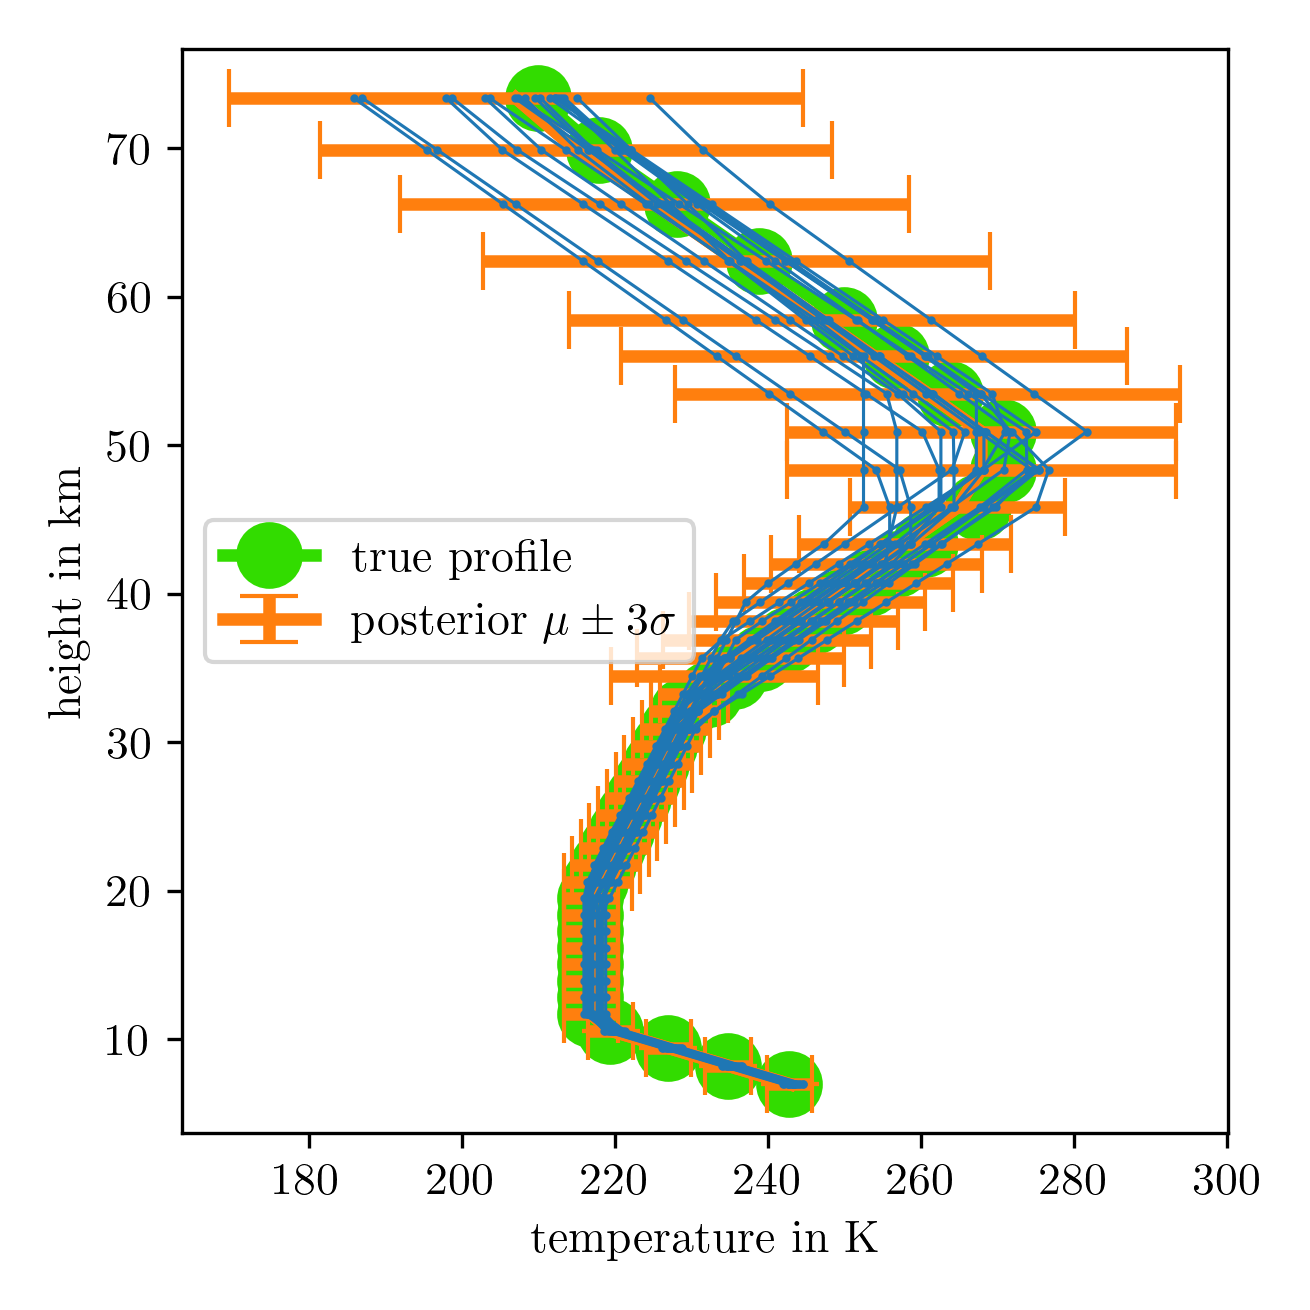
\includegraphics{TempPostMeanSigm.png} 
	\caption[Temperature posterior samples.]{Plot of posterior temperature profiles according to Eq.~\ref{eq:tempFunc} and hyper-parameter samples from the marginal posterior distribution $\pi(\bm{\theta},\lambda,\gamma  | \bm{y})$.}
	\label{fig:TempPost}
\end{figure}
\begin{figure}[ht!]
	\centering
	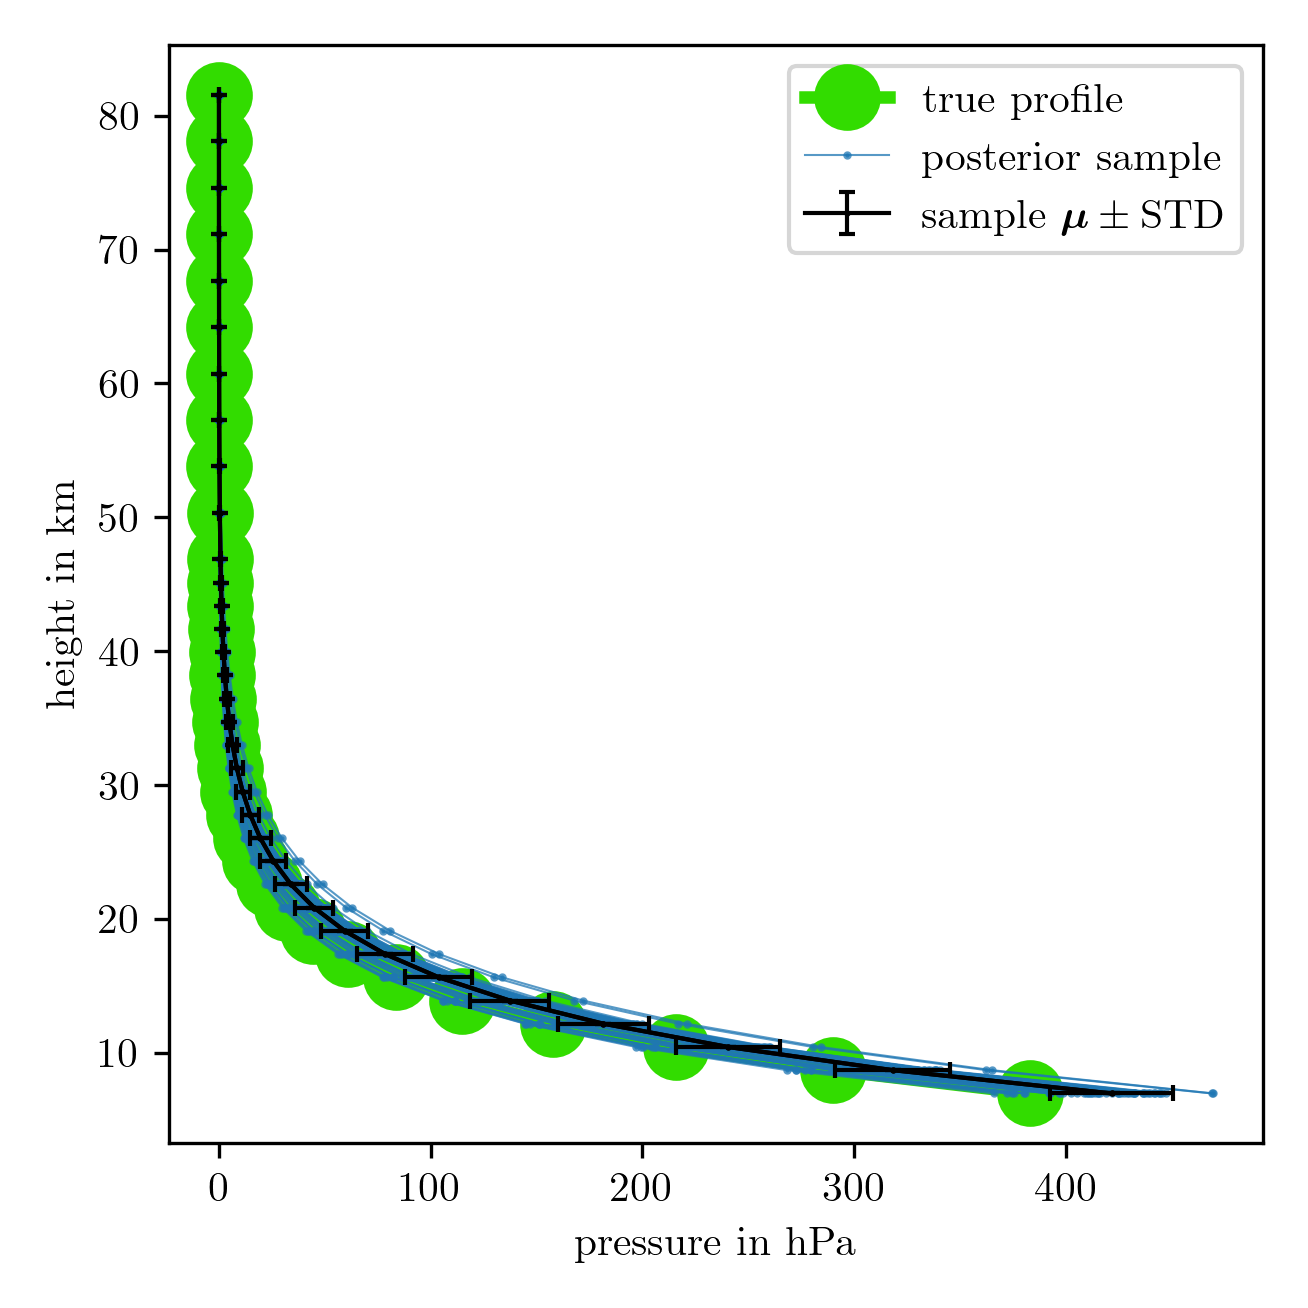
\includegraphics{PressPostMeanSigm.png}
	\caption[Pressure posterior samples.]{Plot of posterior pressure profiles according to Eq.~\ref{eq:pressFunc} and hyper-parameter samples from the marginal posterior distribution $\pi(\bm{\theta},\lambda,\gamma  | \bm{y})$.}
	\label{fig:PressPost}
\end{figure}
\clearpage

\subsection{Full Conditional Posterior -- Ozone}
Due to the large number of hyper-parameters calculating the posterior mean $\bm{\mu}_{\bm{x}|\bm{y}}$ and $\bm{\Sigma}_{\bm{x}|\bm{y}}$ covariance via quadrature as in Eq.~\ref{eq:MeanGenInt} and~\ref{eq:CoVarGenInt} is computationally not feasible.
If the full conditional posterior is a normal distribution, then the randomise then optimise (RTO) method provides a scheme to obtain an independent ozone sample from $\pi(\bm{x}|\bm{\theta}, \delta, \gamma, \bm{y})$ with $\delta = \lambda \, \gamma$.
We introduce the RTO method for general case first and then draw ozone samples from $\bm{x}^{(k)} \sim \pi(\bm{x}|\bm{\theta}^{(k)} , \delta^{(k)} , \gamma^{(k)} , \bm{y})$ conditioned on independent marginal posterior samples $\bm{\theta}^{(k)} , \delta^{(k)} , \gamma^{(k)} \sim \pi(\bm{\theta} , \delta , \gamma | \bm{y})$.


\subsubsection{Randomise then optimise}
\label{subsec:RTO} 
As in~\cite{bardsley2012mcmc} rewrite the full conditional posterior (see Eq.~\ref{eq:CondPostLin}) as
\begin{align}
	\pi(\bm{x} | \bm{\theta},  \delta, \gamma, \bm{y}) & \propto \pi(\bm{y}|\bm{x},  \bm{\theta}, \gamma) \pi(\bm{x}| \delta)\\
	&\propto \exp \left(-\frac{1}{2} (\bm{A}_{\bm{\theta}}  \bm{x} - \bm{y})^T \bm{\Sigma}^{-1}_{\gamma} (\bm{A}_{\bm{\theta}}   \bm{x} - \bm{y})\right) \exp \left(-\frac{1}{2} (\bm{\mu} - \bm{x} )^T \bm{Q}_{\delta}(\bm{\mu} - \bm{x} ) \right),\\
	& = \exp \left( - \frac{1}{2}\left\lVert \hat{\bm{A}} \bm{x} - \hat{\bm{y}} \right\rVert_{L^2}^2 \right),
\end{align}
where
\begin{align}
	\label{eq:minimizer}
	\hat{\bm{A}} \coloneqq 
	\begin{bmatrix}
		\bm{\Sigma}_{\gamma}^{-1/2} \bm{A}_{\bm{\theta}} \ \\
		\bm{Q}_{\delta}^{1/2}
	\end{bmatrix}, \quad 
	\hat{\bm{y}} \coloneqq 
	\begin{bmatrix}
		\bm{\Sigma}_{\gamma}^{-1/2} \bm{y} \\
		\bm{Q}_{\delta}^{1/2} \bm{\mu}
	\end{bmatrix} , 
\end{align}
$\bm{Q}_{\delta}$ is the prior precision, $\bm{\mu}$ the prior mean and $\bm{\Sigma}_{\gamma}$ the noise covariance (see also~\cite{bardsley2014randomize,BardsleyTC2019RTO}).
A sample $\bm{x}^{(k)}$ from the full conditional posterior $ \pi(\bm{x}|   \bm{\theta},  \delta, \gamma,  \bm{y})$ is obtained by minimising the following equation:
\begin{align}
	\bm{x}^{(k)} = \arg \min_{\bm{x}} \lVert \hat{\bm{A}} \bm{x} - ( \hat{\bm{y}} + \bm{b} ) \rVert_{L^2}^2 , \quad \bm{b} \sim \mathcal{N}(\bm{0}, \bm{I}_m) \, ,
\end{align}
where a random perturbation $\bm{b}$ is added.
Similar to Section~\ref{sec:reg}, this expression becomes
\begin{align}
	\label{eq:RTO}
	\left( \bm{A}_{\bm{\theta}}^T \bm{\Sigma}^{-1}_{\gamma} \bm{A}_{\bm{\theta}} + \bm{Q}_{\delta} \right) \bm{x}^{(k)} = \bm{A}_{\bm{\theta}}^T \bm{\Sigma}^{-1}_{\gamma} \bm{y} + \bm{Q}_{\delta} \bm{\mu} + \bm{v}_1 + \bm{v}_2,
\end{align}
%where the term $-\hat{\bm{A}}^T \bm{b}$ is decomposed as $\bm{v}_1 + \bm{v}_2$, 
with $\bm{v}_1 \sim \mathcal{N}(\bm{0}, \bm{A}_{\bm{\theta}}^T \bm{\Sigma}^{-1}_{\gamma} \bm{A}_{\bm{\theta}})$ and $\bm{v}_2 \sim \mathcal{N}(\bm{0}, \bm{Q}_{\delta})$, representing independent Gaussian random variables~\cite{bardsley2012mcmc, fox2016fast}.


\subsubsection{Posterior ozone samples}
More explicitly conditioned on an independent $\bm{\theta}^{(k)},\lambda^{(k)},\gamma^{(k)} \sim \pi(\bm{\theta},\lambda,\gamma | \bm{y})$ and one full conditional posterior sample is given as  
\begin{align}
	\label{eq:RTOAppl}
	\bm{x}^{(k)} = 	\Big(  \underbrace{\gamma^{(k)} \bm{A}_{\bm{\theta}^{(k)}}^T\bm{A}_{\bm{\theta}^{(k)}} +  \delta^{(k)}\bm{L}}_{\bm{B}^{(k)}} \Big)^{-1} \left(  \gamma^{(k)}  \bm{A}_{\bm{\theta}^{(k)}}^T\bm{y} +\sqrt{\gamma^{(k)}} \bm{A}_{\bm{\theta}^{(k)}}^T \bm{v}_1 + \sqrt{\delta^{(k)}}\bm{L}^{1/2}\bm{v}_2\right)
\end{align}
with $\bm{v}_1 \sim \mathcal{N}(\bm{0},  \bm{I}_m )$, $\bm{v}_2 \sim \mathcal{N}(\bm{0}, \bm{I}_n )$, $\bm{Q}_{\delta} = \delta  \bm{L} $, $\bm{\Sigma}^{-1}_{\gamma} = \gamma \bm{I}$ and $\bm{L}^{1/2}$ is the Cholesky decomposition of $\bm{L}$ \cite{bardsley2012mcmc}.
If $n$ is large and calculating the Cholesky decomposition of $\bm{L}$ or constructing $\bm{L}$ is expensive it is recommended to represent $\bm{L}$ as a sum over cliques e.g.,~small $2\times2$ rank-1 matrices (see $\bm{L}$ in Eq.~\ref{eq:LaplRegTheo}).
Then a sample $\bm{v}_2 \sim \mathcal{N}(\bm{0}, \bm{Q}_{\delta})$ can be obtained by drawing $n$ random variables from $\mathcal{N}(0,1)$ without explicitly forming $\bm{L}$~\cite{fox2016fast}.

The Cholesky factorisation of $\bm{B}^{(k)}$ and $\bm{L}$ is obtained via the Python function \texttt{numpy.linalg.cholesky} and \texttt{scipy.linalg.cho\_solve} is used to solve for $\bm{x}^{(k)}$.
We plot 100 samples in Fig.~\ref{fig:O3Post} and a sample mean based on 1000 samples.
The posterior ozone mean is much smaller than the ground truth, especially around the ozone peak.
Compared to the posterior pressure in Fig.~\ref{fig:PressPost}, which is slightly larger than the ground truth, we can conclude that pressure and ozone are highly correlated.
Additionally, the individual posterior samples are more prior-dominated through larger $\lambda$ values (see Fig.~\ref{fig:PostHistTT0}) and hence smoother compared to the previously calculated ozone posterior profiles.
Again, we are not able to recover the second ozone peak at high altitudes.


\begin{figure}[ht!]
	\centering
	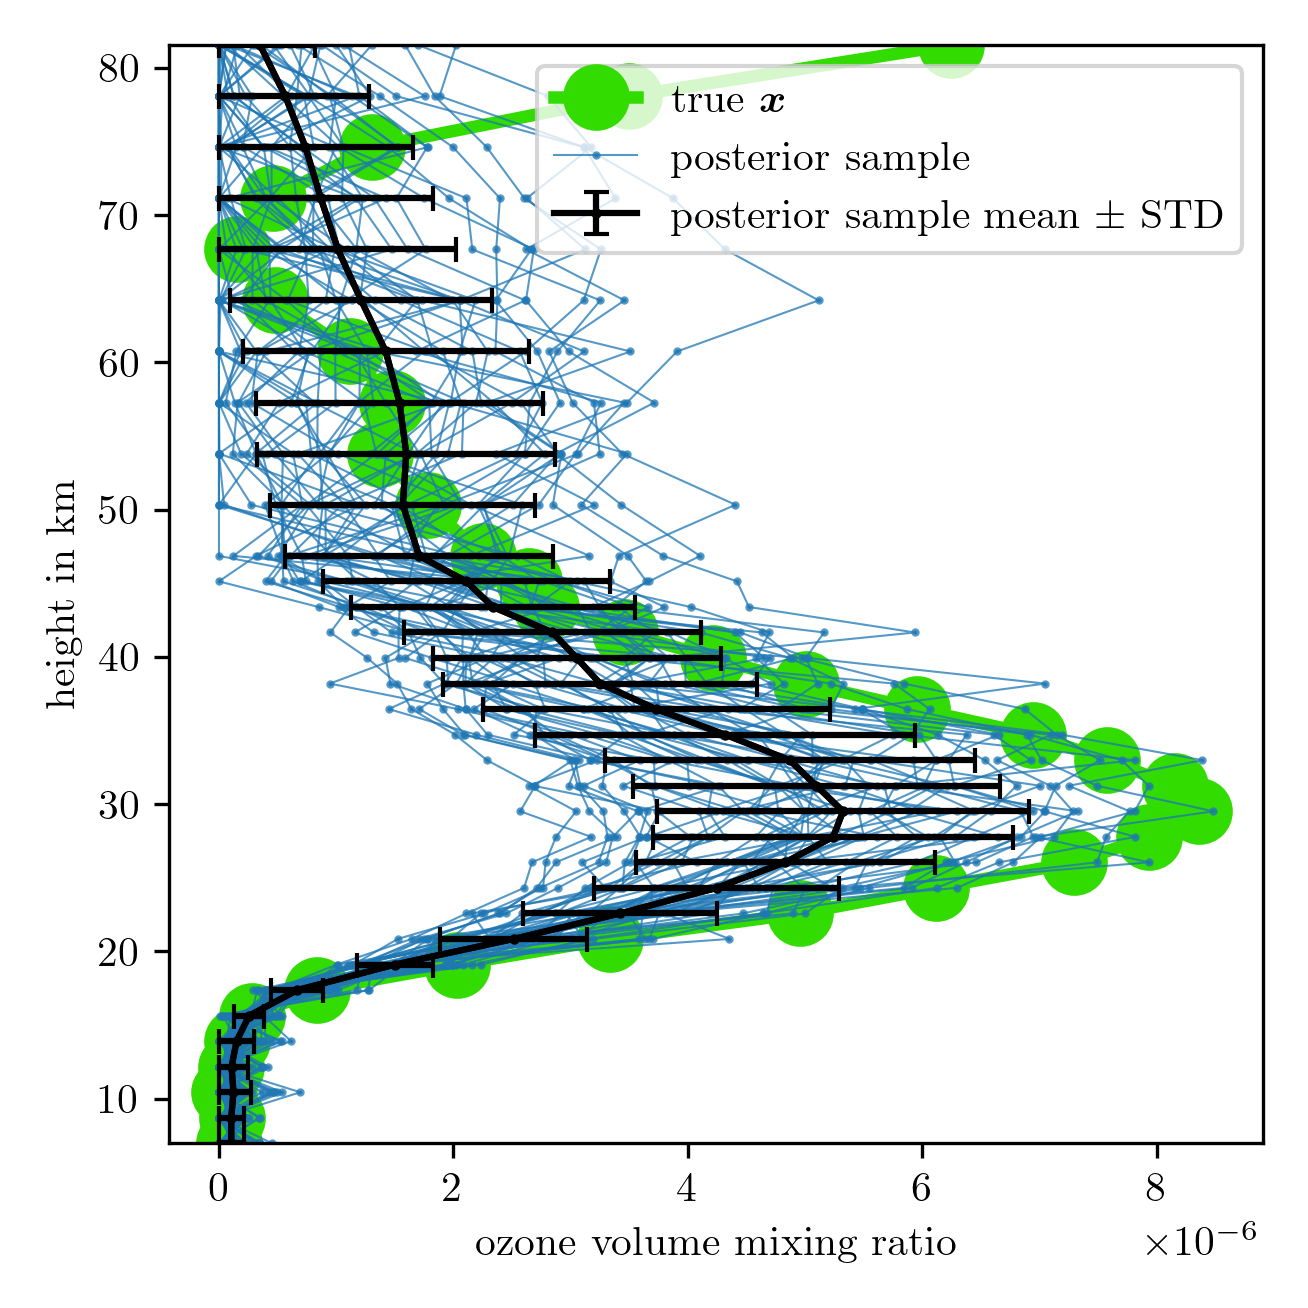
\includegraphics{FullO3Res.png}
	\caption[Pressure posterior samples.]{Plot of ozone samples from the full conditional posterior $\pi(\bm{x} | \bm{\theta},  \delta, \gamma, \bm{y})$ via the RTO method.}
	\label{fig:O3Post}
\end{figure}


\clearpage
%\chapter{Results}

\label{ch:res}

In this chapter we explain how we use the forward model to generate data and how we set up a Bayesian framework to then give distribution of solutions.
Here we make it explicit and proivde all information to be able to replciate our results.
In this work we simulate datawith an ozone profile from \cite{}.
We follow the U.S. standard atmosphere, 1976 \cite{} to relate pressure and temperature and hieght and the HITRANonline \cite{} database to calculate the measured signal.\expandafter\string\the\font 
We follow the mipas instrument description fro the froward model \cite{}.

\section{Simulate Data}
\begin{figure}[ht!]
	\centering
	\input{LIMB.pdf_tex}
	\label{fig:LIMB}
	\caption[Schematic of measurement and analysis geometry.]{Schematic of measurement and analysis geometry, not to scale.
		The stationary satellite, at a constant height $h_\text{sat}$ above Earth, takes $m = 36$ measurements along its line-of-sight defining by the line $\Gamma_j$.
		Each measurement has a limb height $\ell_j$, $j=1,2,\dots,m$ defined as the closest distance of $\Gamma_j$ to the Earth surface, see Fig. \ref{fig:FirstLIMB}.
		Between $h_{L,0} = 7$km and $h_{L,n} = 73.4$km, the stratosphere is discretised into $n =41$ layers as illustrated by the solid green lines.}
\end{figure}


We simulate some data by taking an ozone profile from the retrieval from the MLS limb sounder form \cite{}.
When taking this ozone profile we get given ozone volume mixing ratios and pressure values.
\cite{CubeSatInternal}
\cite{MLSdata}
\cite{vsimevckova2006einstein}
\cite{christentwalkaccess}
\cite{Fox_ISBA2008}
\cite{mipas2000handbook}
\cite{gordon2022hitran2020}
\cite{atmosphere1976us}


%We put the satellite at a constant observe height of $h_{obs} =$ and take $m = $ along the line of sight $\Gamma_j$ in between $h_0= $ and $h_n = $ as requested by Annika et. al. since the pointing accuracy is .
%we assume no signal above and below and that the we have a constant LTE atmosphere in each layer.
%As in section \ref{sec:formodel} the atmosphere is discretised into $n = $ layers
%Where we take the same discretization as given by an ozone profile taken from NASA's (Microwave limb sounder) MLS \cite{}.
%

\subsubsection{Pressure to Height to Temperature}
we relate pressure and height following the book \cite{}where we use the equation
\begin{align}
	\text{d} \ln p= \frac{\text{d}p}{p} = \frac{- g M}{R^* T} \text{d} h \, ,
\end{align}

with the universal gas consant $R^* \approx 8.314  \, \text{N m} / \text{mol} / \text{K}$. The moledus numebr ... is $M = M_0 \approx 28.97 \, \text{kg}/\text{mol}$ for altiudes below 79km \cite{}.
At altitude $h$ the gravitational constant
Up until $86$km we can relate pressure $p$ and geometric height $h$ through the hydrostatic equation

\begin{align}
	g = g_0 \Bigg( \frac{r_0}{r_0 + h} \Bigg) \, ,
\end{align}
with $r_0 \approx 6356 \, \text{km}$ (also known as the polar radius of the earth) and $g_0 \approx 9.81 \text{m}/\text{s}^2$ and \cite{}.


%\begin{itemize}
%	\item what we set
%	\item pointing accuracy number of data set in between atmosphere
%	\item atmospheric layers
%	\item where from ozone profile
%\end{itemize}
%
%
%
%\begin{itemize}
%	\item where from ozone profile
%	\item say what we get form nasa
%	\item assumption for height
%\end{itemize}


%\subsection{Pressure to height}
%\begin{itemize}
%	\item us stabdart atmospher
%	\item assumptions
%\end{itemize}


%\subsection{Hieght to Temperature}
%\begin{itemize}
%	\item us standard atmosphere
%	\item assumptions
%\end{itemize}

We can formulate a temperature function from \cite{atmosphere1976us}
%\begin{align}
%	T(h) = \begin{cases*}
%		T_0, & \text{$h = 0$}\\
%		T_0 + a_0 h , & \text{$0 \leq h < h_{T,1}$}\\
%		T_0 + a_0 h_{T,1}, & \text{$h_{T,1} \leq  h < h_{T,2}$}\\
%		T_0 + a_0 h_{T,1} + a_1 (h   - h_2),  & \text{$h_{T,2} \leq h < h_{T,3}$}\\
%		T_0 + a_0 h_{T,1} + a_1 (h_{T,3} - h_{T,2}) + a_2 (h   - h_3), & \text{$h_{T,3} \leq h < h_{T,4}$}\\
%		T_0 + a_0 h_{T,1} + a_1 (h_{T,3} - h_{T,2}) + a_2 (h_{T,4} - h_{T,3}), & \text{$h_{T,4} \leq h < h_{T,5}$}\\
%		T_0 + a_0 h_{T,1} + a_1 (h_{T,3} - h_{T,2}) + a_2 (h_{T,4} - h_{T,3}) + a_3 (h   - h_{T,5}), & \text{$h_{T,5} \leq h < h_{T,6}$}\\
%		T_0 + a_0 h_{T,1} + a_1 (h_{T,3} - h_{T,2}) + a_2 (h_{T,4} - h_{T,3}) + a_3 (h_{T,6} - h_{T,5}) + a_4 (h - h_{T,6}), & \text{$h_{T,6} \leq h \lesssim 85$}
%	\end{cases*} 
%\label{eq:tempFunc}
%\end{align}
\begin{align}
	T(h) = \begin{cases*}
		T_0, & \text{$h = 0$}\\
		T_0 + a_0 h , & \text{$0 \leq h < h_{1}$}\\
		T_0 + a_0 h_{1}, & \text{$h_{1} \leq  h < h_{2}$}\\
		T_0 + a_0 h_{1} + a_1 (h   - h_2),  & \text{$h_{2} \leq h < h_{3}$}\\
		T_0 + a_0 h_{1} + a_1 (h_{3} - h_{2}) + a_2 (h   - h_3), & \text{$h_{3} \leq h < h_{4}$}\\
		T_0 + a_0 h_{1} + a_1 (h_{3} - h_{2}) + a_2 (h_{4} - h_{3}), & \text{$h_{4} \leq h < h_{5}$}\\
		T_0 + a_0 h_{1} + a_1 (h_{3} - h_{2}) + a_2 (h_{4} - h_{3}) + a_3 (h   - h_{5}), & \text{$h_{5} \leq h < h_{6}$}\\
		T_0 + a_0 h_{1} + a_1 (h_{3} - h_{2}) + a_2 (h_{4} - h_{3}) + a_3 (h_{6} - h_{T5}) + a_4 (h - h_{6}), & \text{$h_{6} \leq h \lesssim 85$}
	\end{cases*} 
	\label{eq:tempFunc}
\end{align}
depending on 12 parameters with values provided by \cite{}, also see table \ref{}.
We set this as our true temperature profile and refer to \cite{} for temperature values above $79 \,\text{km}$.


\subsubsection{Source}
\begin{itemize}
	\item RTE again?
	\item assumptions
\end{itemize}
We calculate the source function $B(\nu, T)$ and the absorption constant $ k(\nu, T)$ as follows.
assumption local thermaodynamic equilibrium
For one species at one specific wave-number the weighted absorption constant becomes
\begin{align}
	\overline{k(\nu, T, r)}    = \sum_{m=1}^{molec} k_m(\nu, T) x_m(r) =  k(\nu, T) x(r) \, ,
\end{align}
with the volume mixing ratio of ozone $x(r)$ at location $r$. 
The absorption constant
\begin{align}
	k(\nu, T) = L(\nu, T_{\text{ref}}) \frac{Q(T_{\text{ref}})}{Q(T)} \frac{ \exp{\{ - c_2 E^{\prime \prime} / T\}} }{\exp{\{ - c_2 E^{\prime \prime} / T_{\text{ref}} \}}} \frac{ 1- \exp{\{ - c_2 \nu  / T \}} }{1 - \exp{\{ - c_2 \nu / T_{\text{ref}} \}}}
\end{align}
is depend on the line intensity $L(\nu, T_{\text{ref}})$ at reference temperature $T_{\text{ref}} =296K $, the lower-state energy of the transition $ E^{\prime \prime} $, the second radiation constant $c2=1.4387769\text{cmK}$ all provided by \cite{}.
Since we only consider one transition namely the lower-state one the partition function becomes
\begin{align}
	Q(T )= g^{\prime \prime} \exp{\{ - \frac{ c_2 E^{\prime \prime} }{T}\}} \, ,
\end{align}
with the the statistical weight $ g^{\prime \prime}$ (also called the degeneracy factor), see \ref{}.
M. Šimečková, D. Jacquemart, L. S. Rothman, R. R. Gamache, and A. Goldman, "Einstein A-coefficients and statistical weights for molecular absorption transitions in the HITRAN database", J. Quant. Spectrosc. Radiat. Transfer 98, 130-155 (2006)

Under the assumption of local thermodynamic (LTE) equilibrium t source function is given by the black body radiation
\begin{align}
	B(\nu,T)   = \frac{2 h c^2 \nu^3}{\exp{\{\frac{hc\nu}{k_B T}\}}-1}\, ,
\end{align}
with Planck's constant $h$, velocity of light $c$ and Boltzmann's constant $k_B$ \cite{}.

Then we can calculate measurement with the RTE in Eq. \ref{eq:RTE} using the trapezoidal rule
\begin{align}
	\label{eq:RTE} 
	y_j =   \int_{\Gamma_j}  B(\nu,T) k(\nu, T)   \frac{p(T)}{k_{\text{B}} T(r)}  x(r)  \tau(r) \text{d}r + \eta_j \, \\
	\tau(r) = \exp{ \Bigl\{ - \int^{r}_{r_\text{obs}}  k(\nu, T)   \frac{p(T)}{k_B T(r^{\prime})}  x(r^{\prime}) \text{d}r^{\prime} \Bigr\} } \, ,\label{eq:absRTE} 
\end{align}

Note we assume infinte spectral resulution and no poisnting errors.
atmopsheric model and now intrumetn model

\section{Bayesian Model and prior analysis}
\begin{itemize}
	\item fill in what we descrube beofre 
	\item describe parametres and hyper paraemrets set up model to make dag
	\item then prior modelling
\end{itemize}
In this section we present the explicit Bayesian we will use to recover pressure temperature and ozone values.

\subsection{DAG}
Again we draw a DAG and specify prior disribtoin over those

\begin{itemize}
	\item correlation structure between ozone and temperature and pressure
\end{itemize}
\begin{figure}[thb!]
	\centering
	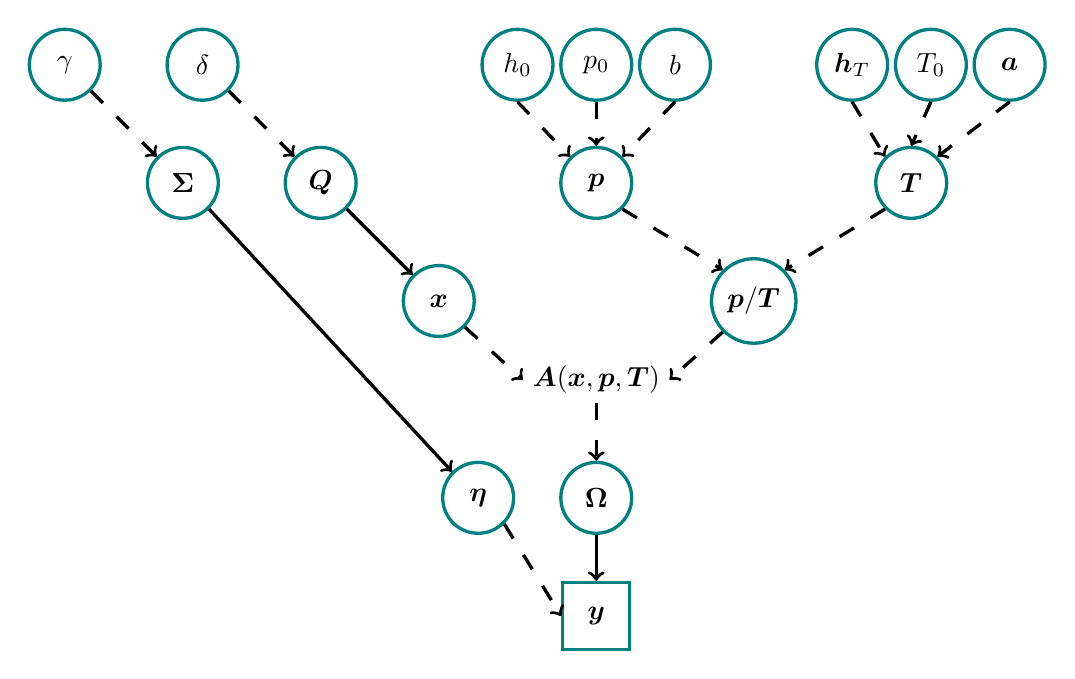
\begin{tikzpicture}
		\node[roundnode2] at (-4.5,6.5) (Q)     {$\bm{Q}$};
		\node[roundnode2] at (-3,5) (x)     {$\bm{x}$};
		\node[align=center] at (-1,4) (A)    {$\bm{A}(\bm{x},\bm{p},\bm{T})$};
		\node[roundnode2] at (-1,2.5) (u)    {$\bm{\Omega}$};
		\node[rectnode] at (-1,1) (y)    {$\bm{y}$};
		\node[roundnode2] at (-2.5,2.5) (e)    {$\bm{\eta}$};
		\node[roundnode2] at (-6.25,6.5) (S)    {$\bm{\Sigma}$};
		\node[roundnode2] at (-7.75,8) (s)    {$\gamma$};
		\node[roundnode2] at (-6,8) (d)    {$\delta$};
		\node[roundnode2] at (3,6.5) (t)     {$\bm{T}$};
		\node[roundnode2] at (-1,6.5) (p)     {$\bm{p}$};
		\node[roundnode2] at (1,5) (pt)     {$\bm{p}/\bm{T}$};
		\node[roundnode2] at (0,8) (b1)    {$b$};
		%\node[roundnode2] at (1,8) (b2)    {$b_2$};
		\node[roundnode2] at (-2,8) (h1)    {$h_{0}$};
		\node[roundnode2] at (-1,8) (p0)    {$p_0$};
		\node[roundnode2] at (2.25,8) (ht)    {$\bm{h}_T$};
		\node[roundnode2] at (3.25,8) (ct)    {$T_0$};
		\node[roundnode2] at (4.25,8) (at)    {$\bm{a}$};
		
		%Lines
		\draw[->, very thick] (S.south east) -- (e.north west);
		\draw[->, mydotted, very thick] (s.south east) -- (S.north west);
		\draw[->, very thick] (u.south) -- (y.north);
		\draw[->, mydotted, very thick] (A.south) -- (u.north);
		\draw[->, mydotted,  very thick] (x.south east) -- (A.west);
		\draw[->, mydotted, very thick] (p.south east) -- (pt.north west);
		\draw[->, mydotted, very thick] (t.south west) -- (pt.north east);
		\draw[->, mydotted, very thick] (pt.south west) -- (A.east);
		\draw[->, mydotted, very thick] (h1.south) -- (p.north west);
		\draw[->, mydotted, very thick] (p0.south) -- (p.north);
		\draw[->, mydotted, very thick] (b1.south) -- (p.north east); 
		%\draw[->, very thick] (b2.south) -- (p.east); 
		\draw[->, mydotted, very thick] (d.south east) -- (Q.north west); 
		\draw[->, mydotted, very thick] (e.south east) -- (y.west); 
		
		\draw[->, very thick] (Q.south east) -- (x.north west); 
		\draw[->, mydotted, very thick] (ht.south) -- (t.north west);
		\draw[->, mydotted, very thick] (ct.south) -- (t.north);
		\draw[->, mydotted, very thick] (at.south) -- (t.north east);
		%\node[align=center] at (0.25,3.95) (f3) {$\approx \bm{M A}_L$};
	\end{tikzpicture} 
\caption[Complete directed acyclic graph of the forward model.]{Complete directed acyclic graph of the forward model. The hyper-parameters at the top deterministically (dotted line) describe the parameters ($\bm{p}/\bm{T}$) or the noise covariance $\bm{\Sigma} = \gamma^{-1} \bm{I}$ of the random (solid line) noise $\bm{\eta} \sim \mathcal{N}(0,\gamma^{-1} \bm{I} ) $ and precision matrix $\bm{Q} = \delta \bm{L}$ of the distribution of $\bm{x}\sim \mathcal{N}(0,\delta \bm{L}) $, where $\bm{L}$ is a graph Laplacian as in Eq. \ref{eq:GLapl}. We can group the noise precision $\gamma$  and the smoothness parameter $\delta$ to define the marginal posterior over those hyper-parameters and then condition on them for the conditional posterior distribution,for further details see Fig. \ref{fig:DAGO3}. In this whole process where we condition on the pressure $\bm{p}$ and temperature $\bm{T}$, which we retrieve separately, see Fig. \ref{fig:DAGPT}. The hyper-parameters $h_0,p_0,b$ deterministically describe the pressure function in Eq. \ref{eq:pressFunc}, note that we only need three parameters here since $h_0< h_{L,0}$ and $\bm{h}= \{ h_1, h_2,h_3,h_4,h_5,h_6\}$, $\bm{a} = \{ a_0, a_1, a_2,a_3,a_4\}$ and $T_0$ determine the temperature function.
The parameters $\bm{x}$ and $\bm{p}/ \bm{T}$ determine the space of all measurable noise free data $\bm{\Omega}$ through the forward model $\bm{A}(\bm{x},\bm{p},\bm{T})$ from which we randomly observe data set plus some random noise.}
\label{fig:DAGComplete}
\end{figure}

\subsection{Prior Modelling}
\begin{itemize}
	\item physical meaning by choosing priors
	\item eventuel depednices
	\item draw samples form priors should be as loose as possible
\end{itemize}
\begin{table}
	\centering
	\begin{tabular}{ |c||c|c|c|c|   }
		\hline
		& &\multicolumn{2}{|c|}{TT bounds}&\\
		\hline
		model parameters& priors&\makecell{lower}& \makecell{upper\\
		}&Context\\
		\hhline{|=||=|=|=|=|}
		$\gamma$ & $\mathcal{T}(1,10^{-10})$ &$10^{-8}$ &$4 \cdot 10^{-7}$& $\bm{y}$\\ \hline
		$\delta$ &$\mathcal{T}(1,10^{-10})$ & -&-& $\bm{x}$\\ \hline
		$\lambda$ &- & 150&5000& $\bm{x}$\\ \hline
		$\bm{x}$ &$\mathcal{N}(0,\delta \bm{L})$ & -&-& $\bm{x}$\\ \hhline{|=||=|=|=|=|}
		%$\gamma$ & $\mathcal{N}(2.58e-9,2.58e-11)$ &2.45e-9&2.7e-9 &$\bm{x}$\\
		%$\delta_0$ &  $\mathcal{N}(0.8e-4,0.75e-5)$& 4e-5 & 1.1e-4&$\bm{x}$\\
		%$a_0$ &  $\mathcal{T}(3,1e6)$& 1e-15&1e-5&$\bm{x}$\\ \hline
		%$h_0$ &  $\mathcal{N}(31.35,1)$&27 &35&$\bm{x}$\\ \hline
		$h_0$ &  $\mathcal{N}(6,0.6)$& 5.3&6.1&$\bm{p/T}$\\ \hline
		$p_0$ &  $\mathcal{N}(460,4)$&443 &471&$\bm{p/T}$\\ \hline
		$b$ &  $\mathcal{N}(0.167,5 \cdot 10^{-4})$& 0.166& 0.169 &$\bm{p/T}$\\ \hline
		%$b_2$ & $\mathcal{N}(0.13,0.067)$& 0&0.32&$\bm{p/T}$\\ \hline
		$h_{1}$ &  $\mathcal{N}(11,0.5)$&10.6 &11.3&$\bm{p/T}$\\ \hline
		$h_{2}$ &  $\mathcal{N}(20,3)$&16.6 &22.7&$\bm{p/T}$\\ \hline
		$h_{3}$ &  $\mathcal{N}(32,1)$&23.6 &43.3&$\bm{p/T}$\\ \hline
		$h_{4}$ &  $\mathcal{N}(47,2)$&45.2 &48.9&$\bm{p/T}$\\ \hline
		$h_{5}$ &  $\mathcal{N}(51,2)$&49.2 &52.9&$\bm{p/T}$\\ \hline
		$h_{6}$ &  $\mathcal{N}(71,2)$&57.8 &84.1&$\bm{p/T}$\\ \hline
		$a_{0}$ &  $\mathcal{N}(-6.5,0.01)$&-6.54 &-6.46&$\bm{p/T}$\\ \hline
		$a_{1}$ &  $\mathcal{N}(1,0.01)$&0.96 &1.04&$\bm{p/T}$\\ \hline
		$a_{2}$ &  $\mathcal{N}(2.8,0.1)$&2.43 &3.18&$\bm{p/T}$\\ \hline
		$a_{3}$ &  $\mathcal{N}(-2.8,0.01)$&-3.18 &-2.43&$\bm{p/T}$\\ \hline
		$a_{4}$ & $\mathcal{N}(-2,0.01)$ &-2.04 &-1.96&$\bm{p/T}$\\ \hline
		$T_{0}$ &  $\mathcal{N}(288.15,2)$& 282 &295&$\bm{p/T}$\\
		\hline
	\end{tabular}
	\caption{Gaussian $\mathcal{N}(\mu,\sigma)$ and gamma distribution $\mathcal{T}(\alpha = \text{scale}, \beta = \text{rate})$
		Bounds for t and p 2.8 times the variance around the mean
		round pressure approx and  test if would work with previous gamma prior or fix gamma prior with set values}
	\label{tab:priors}
\end{table}

In practise we sperate OPzone and conditoin on tempreature and pressure  or vice versa. 
\subsubsection{Ozone}
graph lacoiacn 
wigthing in between
similiar to a ciuop;led osscialtors
what heught is change of weights
\begin{align}
	\bm{Q}= \delta \bm{L} =
	\delta
	\begin{bmatrix}
		2 & -1 & & &  \\
		-1 & 2 & -1 & &   \\
		& \ddots & \ddots & \ddots &\\ 
		&   & -1 & 6 & -5 \\
		& & & \ddots & \ddots & \ddots  \\ 
		& & & &  -5 & 10 & -5 \\
		& & & & & -5 & 10 
	\end{bmatrix} 
\label{eq:GLapl} 
\end{align}
\begin{figure}[ht!]
	\centering
	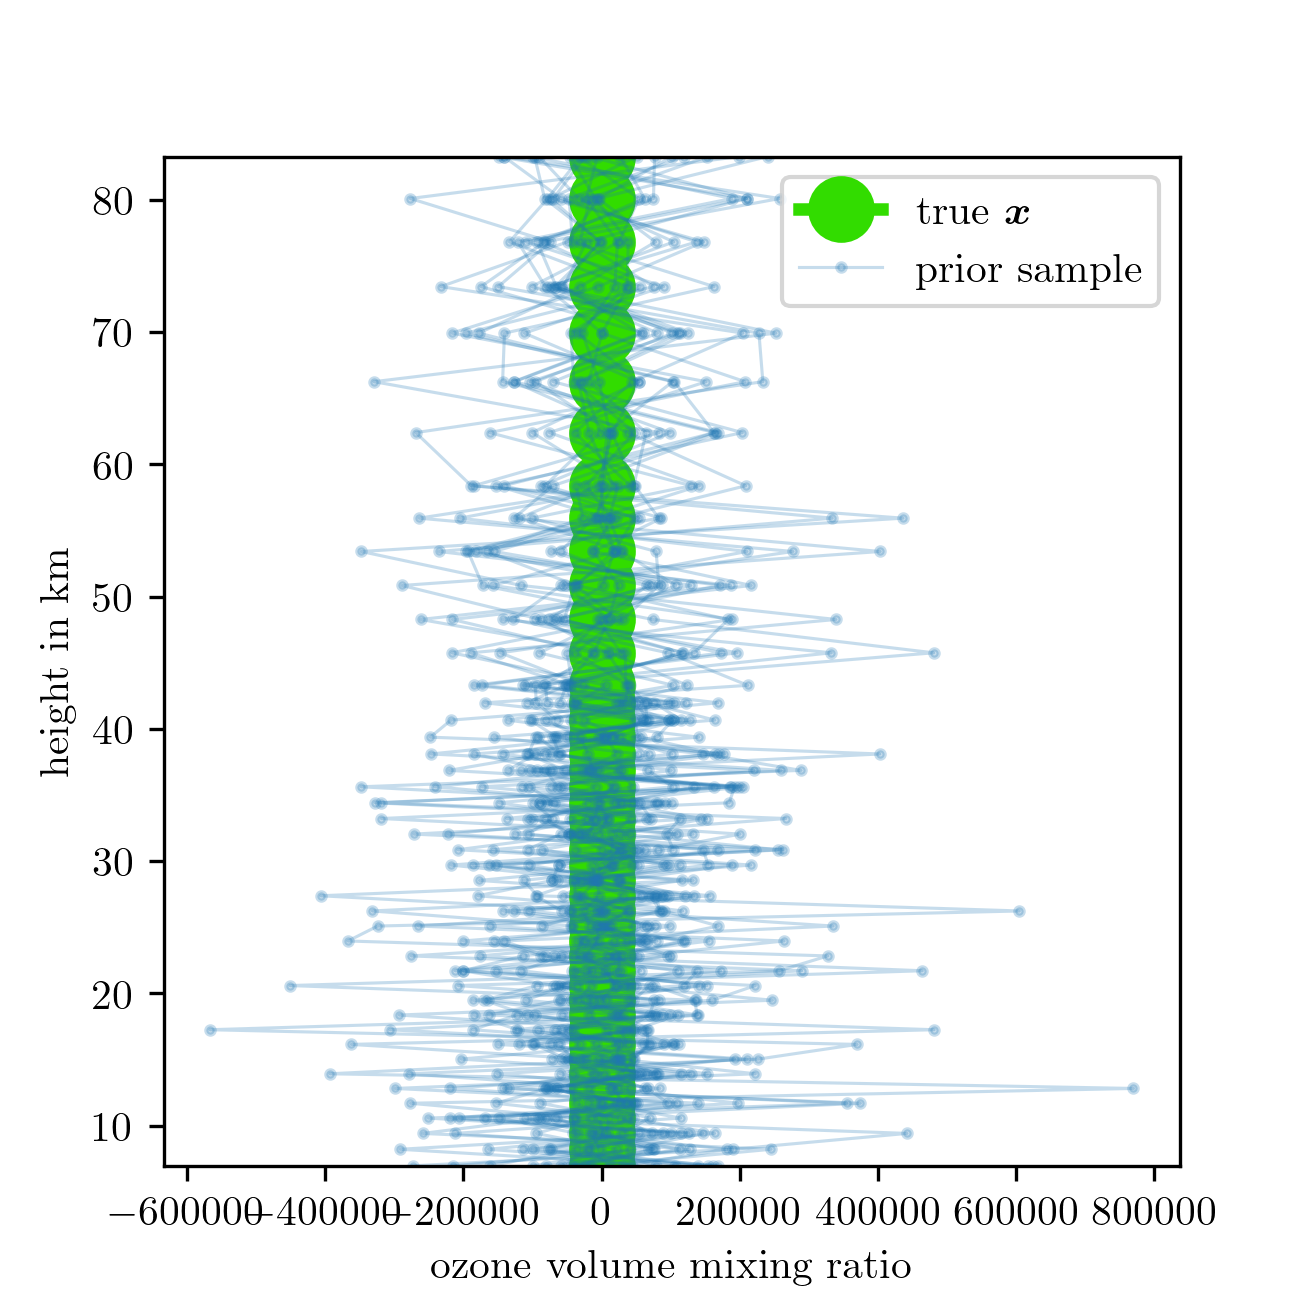
\includegraphics{OzonePrior.png}
	\caption[Samples from ozone prior distribution.]{We draw samples from ozone prior distribution $\bm{x} \sim \mathcal{N}(0,\delta \bm{L})$ after generating a sample from the hyper-prior distribution $\delta \sim \mathcal{T}(1,10^{-10})$. Note that since the spread/variance of prior samples is very large compared to the ozone volume mixing ratios, the ozone profile appears to be constant, which it is not, as seen e.g. in Fig. \ref{fig:O3Samp}.}
	\label{fig:O3Prior}
\end{figure}
\subsubsection{pressure over temperature}
We parametrize the pressure by fitting one exponential to the pressure values $p$ related to the height $h$ by Eq. \ref{}.

The pressure function,
\begin{align}
	p(h) =
	\exp{ \{ -b \,  (h - h_{0} ) \} } \,  p_0 \, ,
	\label{eq:pressFunc}
\end{align}
is depending on three different parameters, the gradient $a_{p,1}$ and the tuple $(p_0,h_{p,0})$.


\begin{itemize}
	\item show that pressure is dominant
	\item correlation structure
	\item appendix
\end{itemize}

PriorTempOverPostMeanSigm



\begin{figure}[ht!]
	\centering
	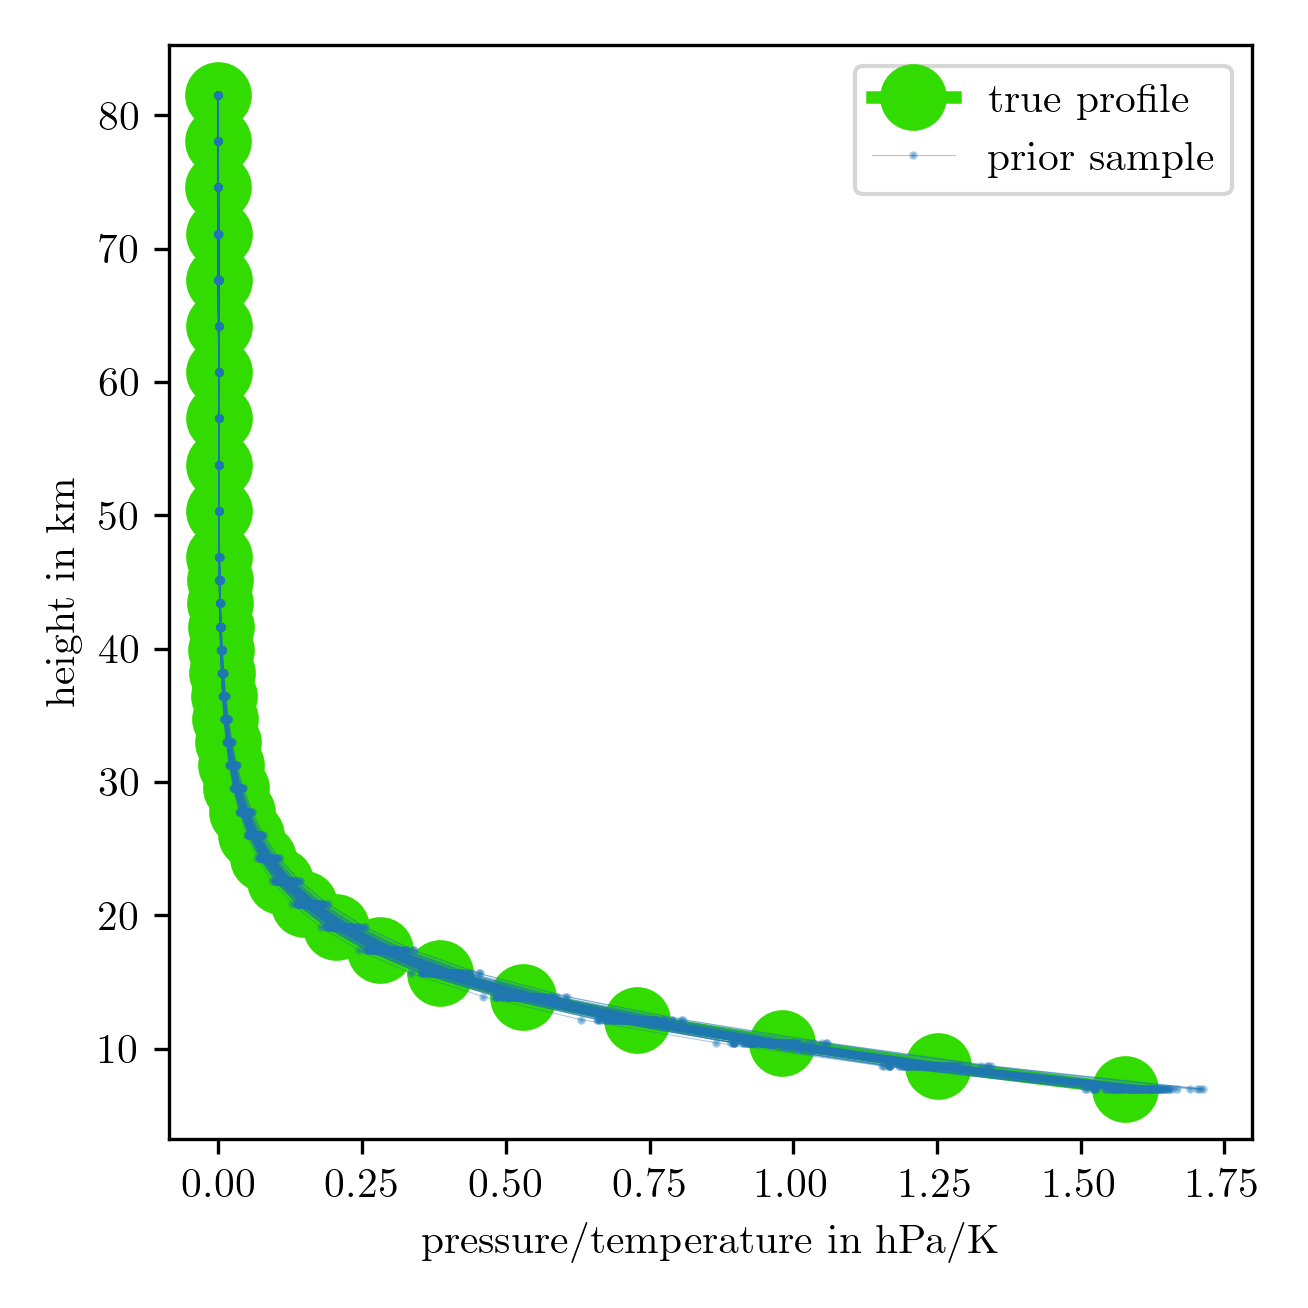
\includegraphics{PriorTempOverPostMeanSigm.png}
	\caption[Prior Samples of $\bm{p}/\bm{T}$ according to the respective hyper-prior distribution.]{We draw samples from the hyper-prior distribution of $h_0, b, p_0, h_1, h_2,h_3,h_4,h_5,h_6, a_0, a_1, a_2,a_3,a_4$ and $T_0$ as defined in table \ref{tab:priors} and then calculate $\bm{p}/\bm{T}$ according to the functions in Eq. \ref{eq:pressFunc} and \ref{eq:tempFunc}.}
	\label{fig:PriorPressOverTemp}
\end{figure}

\begin{figure}[ht!]
	\centering
	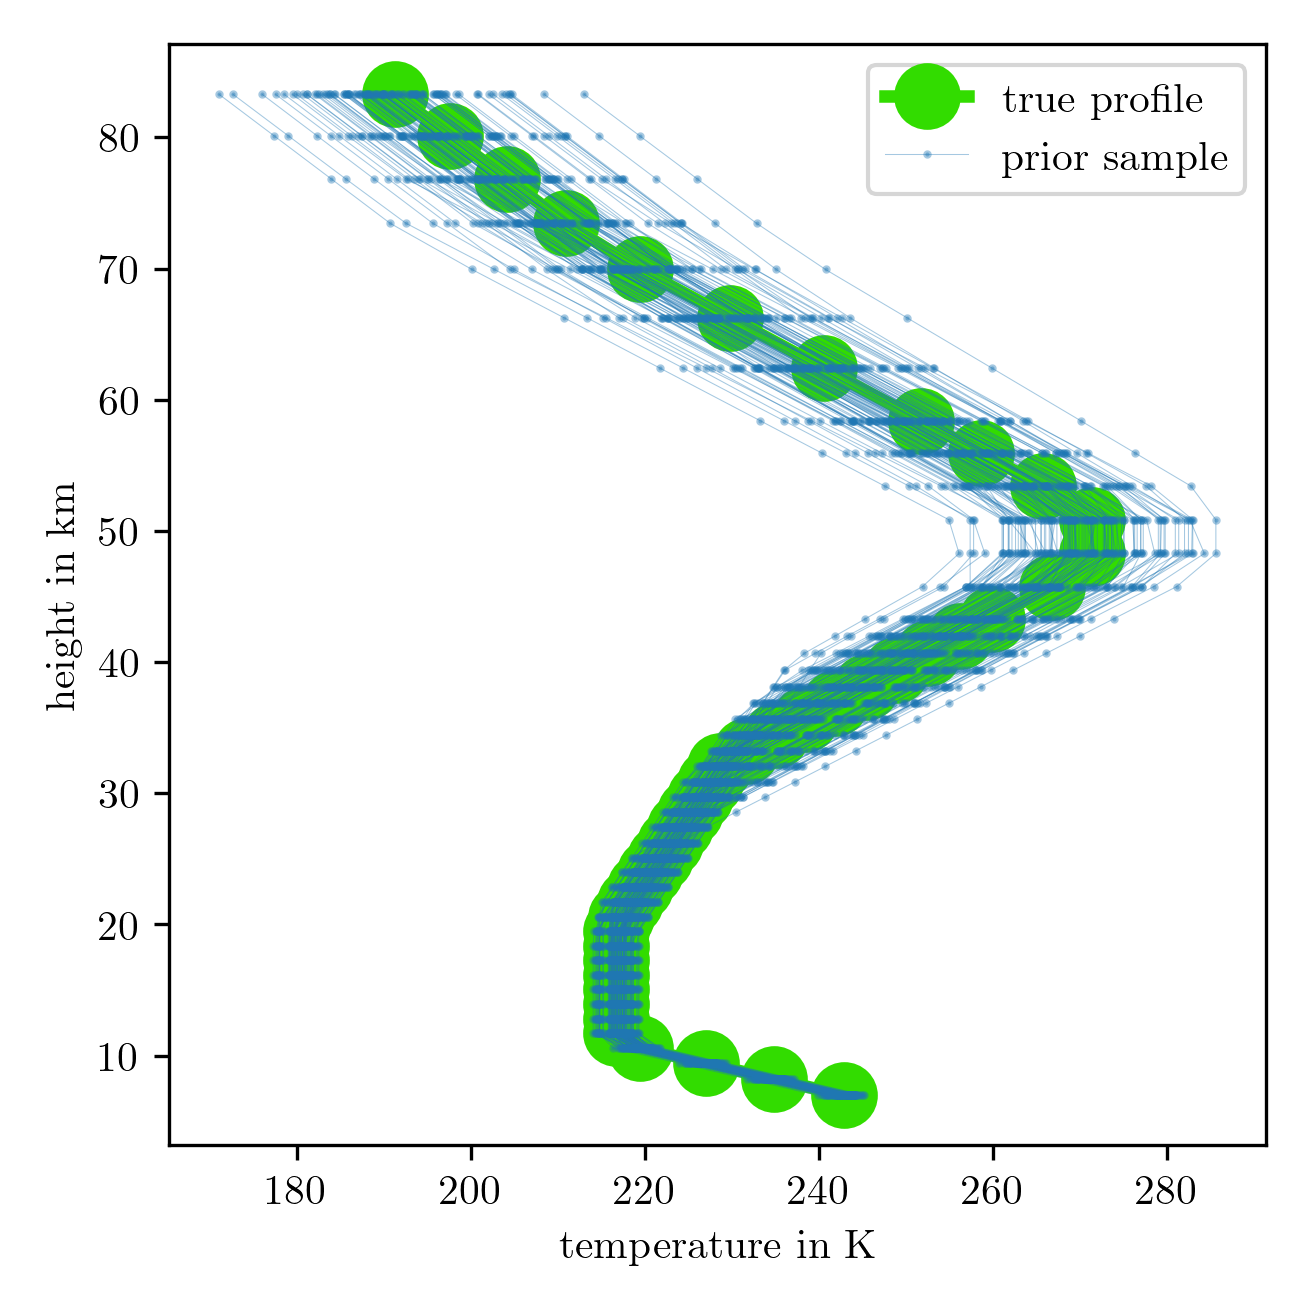
\includegraphics{PriorTempPostMeanSigm.png}
	\caption[Prior Samples of $\bm{T}$ according to the respective hyper-prior distribution.]{We draw samples from the hyper-prior distribution of $h_1, h_2,h_3,h_4,h_5,h_6, a_0, a_1, a_2,a_3,a_4$ and $T_0$ as defined in table \ref{tab:priors} and then calculate $\bm{T}$ according to the function in Eq. \ref{eq:tempFunc}.}
	\label{fig:PriorTemp}
\end{figure}

\begin{figure}[ht!]
	\centering
	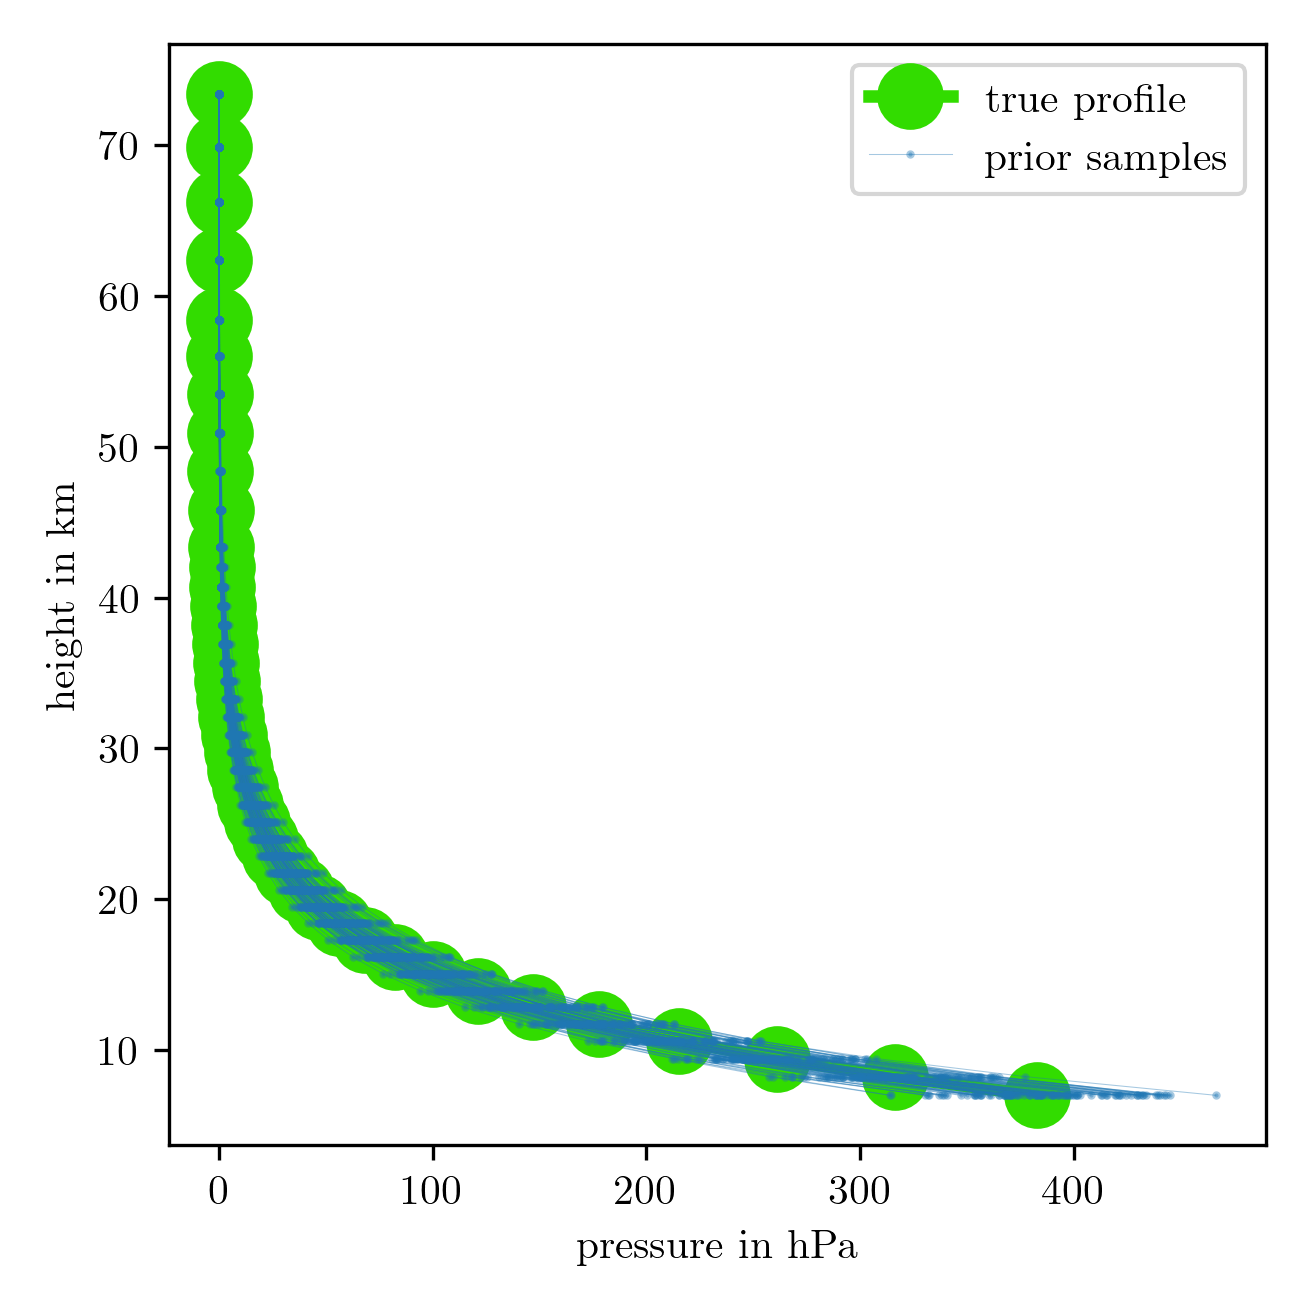
\includegraphics{PriorPressPostMeanSigm.png}
	\caption[Prior Samples of $\bm{p}$ according to the respective hyper-prior distribution.]{We draw samples from the hyper-prior distribution of $h_0, b$ and $p_0$ as defined in table \ref{tab:priors} and then calculate $\bm{p}$ according to the function in Eq. \ref{eq:pressFunc}.}
	\label{fig:PriorPress}
\end{figure}


\subsection{Posterior distributions}
\begin{itemize}
	\item explain where we use MTC and that T/p is spereate
	\item marginal posterior, noise and covarince and perciosn matrix
	\item picture of f and g
	\item taylor expansion
	\item maybe make  metroplis explixit
\end{itemize}
conditioned on a ozone profile
\subsubsection{pressure over temperature}

conditioned on a temperauter opver pressure profile
\subsubsection{Ozone -- marginal posterior}
\section{MTC posterior sampling}
\label{sec:postsamp}
In this Section we discuss sampling from the posterior distribution. But you don't need to.
\subsection{Sampling from the marginal posterior distribution over hyper-parameters}
%In this section we present two algorithm to sample from the marginal posterior distribution.
Now, to sample from the marginal posterior of the hyper-parameters
% and the posterior distribution of the parameters condition on the hyper-parameter $\pi(\bm{x}|\bm{y}, \lambda, \gamma )$, with $\lambda = \delta / \gamma$.
\begin{align}
	\pi(\lambda, \gamma | \bm{y})
	\propto  \lambda^{n/2} \gamma^{m/2}   \exp{ \Bigl\{ - \frac{1}{2} g ( \lambda) - \frac{\gamma}{2} f ( \lambda) \Bigr\} } \pi(\lambda, \gamma),
	\label{eq:MargPostAppl}
\end{align}
with $\lambda = \delta / \gamma$,
\begin{subequations}
	\label{eq:fandg}
	\begin{align}
		&f ( \lambda) = \bm{y}^T \bm{y} - (\bm{A}^T \bm{y})^T (\bm{A}^T  \bm{A} + \lambda \bm{L})^{-1} (\bm{A}^T \bm{y})  \, ,  \\
		&\text{and } g(\lambda) = \log \det (\bm{A}^T  \bm{A} + \lambda \bm{L}) \,.
	\end{align}
\end{subequations}
we employ a so-called MWG (Metropolis within Gibbs) algorithm, summarised in the algorithmic Box $1$.
One may implement a Metropolis random walk on the full conditional
\begin{align}
	\label{eq:lamCondPrior}
	\pi(\lambda | \bm{y}, \gamma) &\propto \lambda^{n/2+\alpha_\delta -1} \exp{\Bigl\{ - \frac{1}{2} g ( \lambda) - \frac{\gamma}{2} f ( \lambda) - \beta_\delta \gamma \lambda \Bigr\}} 
\end{align} 
and do a Gibbs steps on
\begin{align}
	\gamma |  \bm{y}, \lambda &\sim \Gamma \bigg( \frac{m}{2} + \alpha_\delta + \alpha_\gamma, \frac{1}{2} f (\lambda ) + \beta_\gamma + \beta_\delta \lambda \bigg)\label{eq:gamCondPrior}
\end{align} 
to generate marginal posterior samples $(\lambda, \gamma)^{(1)}, \dots, (\lambda, \gamma)^{(N)} \sim  \pi(\lambda, \gamma| \bm{y})$.
Note that, when changing variables from $\delta = \lambda \gamma$ to $\lambda$ the hyper-prior distribution changes to $\pi(\lambda) \propto \lambda^{\alpha_\delta-1} \gamma^{\alpha_\delta} \exp{(- \beta_\delta \lambda  \gamma)} $, due to $\text{d}\delta / \text{d} \lambda = \gamma$.
We find the full conditionals by factorisation.



As part of the Metropolis random walk, a new $\lambda^\prime$ given the previous $\lambda^{(k)}$, with $k = 1 , \dots, N$, is proposed according to the distribution $q(\lambda^\prime|\lambda^{(k)}) \sim \mathcal{N}(\lambda^{(k)}, w_\lambda)$.
The proposed sample is rejected or accepted with the acceptance probability $\alpha(\lambda^\prime |\lambda^{(k)})$, see Equation \eqref{eq:alpha}.
Here, calculating the difference $\Delta f = f(\lambda^\prime) - f(\lambda^{(k)})$ and $\Delta g = g(\lambda^\prime) - g(\lambda^{(k)})$ is crucial.
Since the functions $f(\lambda)$ and $g(\lambda)$ are well-behaved over a large range of $\lambda$ and almost linear around the mode of the marginal posterior $\lambda_0$, a Taylor expansion around the mode is sufficient, see Figure \ref{fig:f_and_g}.
Then, computing the acceptance ratio does not involve evaluating $f(\lambda)$ and $g(\lambda)$, but the difference $\Delta f = \sum f^{(r)}(\lambda_0) (\lambda^\prime - \lambda^{(k)})^r$ and $\Delta g = \sum g^{(r)}(\lambda_0) (\lambda^\prime - \lambda^{(k)})^{r}$.
The derivatives are
\begin{align}
	f^{(r)}& (\lambda_0)= (-1)^{r+1} r! (\bm{A}^T \bm{y})^T (\bm{B}_0^{-1} \bm{L})^r \bm{B}_0^{-1} \bm{A}^T \bm{y} \label{eq:ftay}  \\
	\text{and } &g^{(r)} ( \lambda_0) = (-1)^{r+1} \, \text{tr} \big( (\bm{B}_0^{-1}\bm{ L })^r \big)
	\label{eq:gtay}
\end{align} 
with $\bm{B}_0 = \bm{A}^T  \bm{A} + \lambda_0 \bm{L}$.

Finally, a Gibbs step provides a new $\gamma^{(k+1)} \sim \gamma | \bm{y}, \lambda^{(k+1)}$, see Equation \eqref{eq:GibbsStep}.


\subsubsection{Ozone -- conditional posterior}

Conditioned on the hyper-parameters $\bm{\theta} = ( \delta, \gamma)$ we utilise the so-called RTO (randomize then optimize) method \cite{bardsley2012mcmc,bardsley2015randomize, fox2016fast} to draw an independent sample of the conditional posterior distribution.
By perturbation of the exponent of
\begin{align}
	\bm{x}| \bm{y} ,\delta, \gamma \sim \mathcal{N}\big(  (\bm{A}^T \bm{A} + \delta / \gamma \bm{L} )^{-1} \bm{A}^T \bm{y}, (\gamma \bm{A}^T \bm{A} + \delta \bm{L} )^{-1} \big) \, \label{eq:CondPost},
\end{align}
we obtain one independent sample $\bm{x} \sim \pi(\bm{x}|\bm{y}, \bm{\theta})$ for each solve of Equation \eqref{eq:RTO}, see algorithmic Box $2$.


We use the same discretization of the atmosphere as given by the ozone profile taken from \cite{MLSdata} \url{https://disc.gsfc.nasa.gov/datasets/ML2O3_005/summary?keywords=mls%20o3}.
We use ozone values between a height of $10$km up to $38$km, which results in $n=37$ layers.
We set the number of measurements to $m= 105 $.
(I can't think of any good reason why I chose that, it is a good number not too big not too small and gives consistent results for various datasets)\\

When finding the mode we use the scipy.optimize.fmin function and limit the number of function evaluations to 25.
We use Cholesky factorisation to evaluate $g(\lambda)$ and $f(\lambda)$ and to construct the coefficients of the Taylor series, where we have to calculate  $\bm{B}^{-1} \bm{L} $ and  $\bm{B}^{-1}  \bm{A}^T \bm{y}$ once at $\lambda_0$.\\


We bin the samples into a normalised histogram and use the height of the bars as quadrature weights $\pi(\lambda_i| \bm{y})$, where the quadrature point $\lambda_i$ denotes the centre of each bin.
To calculate the conditional posterior mean we use approximate quadrature
\begin{align}
	\mu_{\bm{x}|\bm{y}} = \int x_{\lambda} \pi(\lambda| \bm{y}) \text{d}\lambda \approx \sum x_{\lambda_i} \pi(\lambda_i| \bm{y}) \, ,
\end{align}
with $\sum \pi(\lambda_i| \bm{y}) = 1$, so that the integral can be interpreted as the weighted average.
See Sec. 2.1
\cite{Dick_Kuo_Sloan_2013} \url{https://www.cambridge.org/core/journals/acta-numerica/article/highdimensional-integration-the-quasimonte-carlo-way/03F126DDF465F915B22D5D709CD28946}.\\

We bin the samples into $3$ bins and stop increasing the number of bins by one if the relative error between the previous and the current conditional posterior mean is less than $0.1\%$.
This gives a total number of $3+4+5 = 12$ solves for $x_{\lambda}$.
In addition, we calculate the covariance matrix $(\gamma \bm{B}_{\lambda})^{-1} $, where we use Cholesky factorisation to invert $\bm{B}$, solving the integral
\begin{align}
	\Sigma_{\bm{x}|\bm{y}} = \int \gamma^{-1}  \pi(\gamma | \bm{y} ) \, \text{d} \gamma \, \int  \bm{B}_{\lambda}^{-1} \, \pi(\lambda | \bm{y} )  \, \text{d} \lambda  \approx \sum {\gamma_i}^{-1}\pi(\gamma_i| \bm{y}) \sum \bm{B}_{\lambda_i}^{-1}\pi(\lambda_i| \bm{y})\, .
\end{align}\\

It takes us less than 0.1s to draw 10000 samples from the marginal posterior and to calculate the conditional posterior mean or to solve for 200 different $x_{\lambda}$ and to find the regularised solution at the point of maximum curvature using the kneedle algorithm.\\


\section{Affine Map} 
\label{sec:affineMap}
\begin{itemize}
	\item introduce affine sapce and how we get affine map, to motivate samples from posterir space
	\item explicit, why we need ozone profiles, because it is faster and temperature and pressure are more well defined within the atmosphere
	\item generate affine space every samples is a feasable sample
	\item generate data without noise to find affine map
\end{itemize}
We do MTC with linear forward map no updadeted
In this specific case we find the affine map
\begin{align}
	\bm{M} = \begin{bmatrix}
		\text{---} & \bm{M}_0 &   \text{---}  \\
		&  \vdots  & \\
		\text{---}& \bm{M}_j &  \text{---} \\
		&  \vdots  & \\
		\text{---} & \bm{M}_m &   \text{---}
	\end{bmatrix} \, \in \mathbb{R}^{m \times m} ,
\end{align}
with rows $\bm{M}_j$ using a linear solver for
\begin{align}
	W \bm{M}_j^\top \, = V_{j} \, .
\end{align}
Here $V_j$ denotes the $j$th row of  
\begin{align}
	V = \begin{bmatrix}
		\vert&   &  \vert & & \vert \\
		\bm{A}_{NL} (\bm{x}^{(1)} ) &  \cdots& \bm{A}_{NL} (\bm{x}^{(j)} )&  \cdots & \bm{A}_{NL} (\bm{x}^{(m)})  \\
		\vert&   &  \vert & & \vert 
	\end{bmatrix}
\end{align}
and
\begin{align}
	W = \begin{bmatrix}
		\vert&   &  \vert & & \vert \\
		\bm{A}_{L} \bm{x}^{(1)} &  \cdots& \bm{A}_{L} \bm{x}^{(j)} &  \cdots & \bm{A}_{L} \bm{x}^{(m)} \\
		\vert&   &  \vert & & \vert 
	\end{bmatrix}
\end{align}
is a $\mathbb{R}^{m \times m} $ matrix as well as $\bm{A}_{NL}$.
Then the non-linear forward model can be approximated so that
\begin{align}
	\bm{A}_{NL}(\bm{x}) \approx \bm{M A}_L \bm{x}\, .
\end{align}

\subsection{First MTC}
\begin{itemize}
	\item make table with set up for TT and sampling , number of samples
	\item normalize in evrey step
	\item we use RTO to generate samples
\end{itemize}
\begin{figure}[thb!]
	\centering
	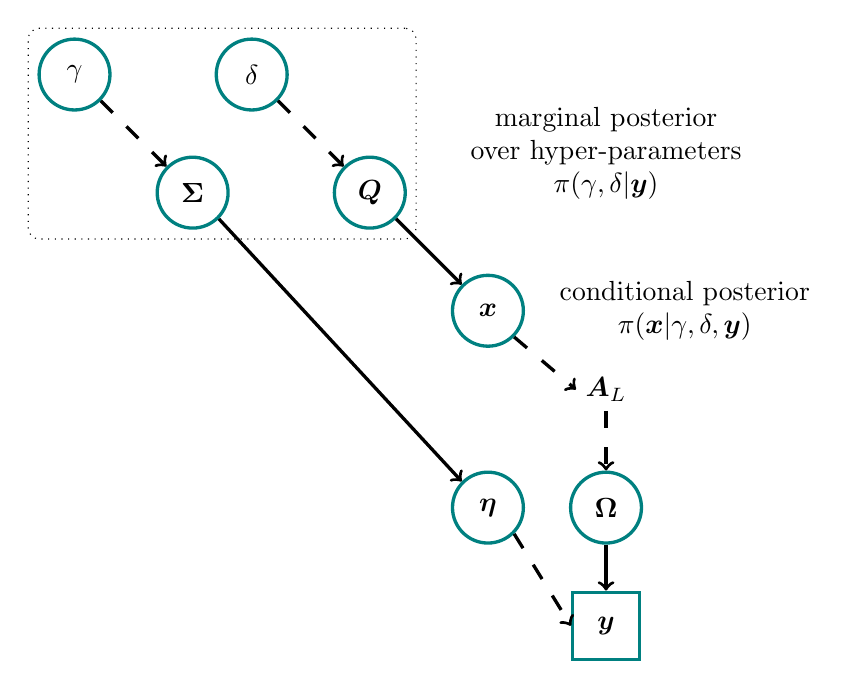
\begin{tikzpicture}
		\node[roundnode2] at (-4,6.5) (Q)     {$\bm{Q}$};
	\node[roundnode2] at (-2.5,5) (x)     {$\bm{x}$};
	\node[align=center] at (-1,4) (A)    {$\bm{A}_L$};
\node[roundnode2] at (-1,2.5) (u)    {$\bm{\Omega}$};
\node[rectnode] at (-1,1) (y)    {$\bm{y}$};
\node[roundnode2] at (-2.5,2.5) (e)    {$\bm{\eta}$};
\node[roundnode2] at (-6.25,6.5) (S)    {$\bm{\Sigma}$};
\node[roundnode2] at (-7.75,8) (s)    {$\gamma$};
\node[roundnode2] at (-5.5,8) (d)    {$\delta$};
		
	%Lines
	\draw[->, very thick] (S.south east) -- (e.north west);
	\draw[->, mydotted, very thick] (s.south east) -- (S.north west);
		\draw[->, mydotted, very thick] (e.south east) -- (y.west);
	\draw[->, very thick] (u.south) -- (y.north);
	\draw[->, mydotted, very thick] (A.south) -- (u.north);
	\draw[->, mydotted,  very thick] (x.south east) -- (A.west);
	
	\draw[->, mydotted, very thick] (d.south east) -- (Q.north west); 
	
	\draw[->, very thick] (Q.south east) -- (x.north west); 
	%\node[align=center] at (0,4) (f3) {$= \bm{A}$};
	%\node[align=center] at (0.25,3.95) (f3) {$\approx \bm{M A}_L$};
	\node[align =center] at (-1,7) (T1) {marginal posterior \\ over hyper-parameters \\ $\pi(\gamma, \delta | \bm{y})$};
	\node[align =center] at (0,5) (T1) {conditional posterior \\ $\pi( \bm{x} |\gamma, \delta, \bm{y})$ };

	
	\node[fit=(S)(s)(Q)(d),draw,dotted,black, rounded corners] {};
	\end{tikzpicture} 
\caption[Directed acyclic graph for ozone retrieval and MTC scheme.]{Directed acyclic graph for ozone retrieval and MTC scheme as described in Fig. \ref{fig:DAGComplete}. The hyper-parameters $\delta$ and $\gamma$ determine the noise covariance $\bm{\Sigma}$ for the random noise vector $\bm{\eta} \sim \mathcal{N}(0, \gamma^{-1}\bm{I})$ and the prior precision matrix $\bm{Q} = \delta \bm{L}$ for the distribution over $\bm{x} \sim \mathcal{N}(0, \delta \bm{L})$, where $\bm{L}$ is the graph Laplacian, see Eq. \ref{eq:GLapl}. In the MTC scheme we evaluate the marginal posterior over the hyper-parameters $\pi(\gamma, \delta | \bm{y})$ as in Eq. \ref{eq:} first and then conditional posterior $\pi(\bm{x}|\gamma,\delta,\bm{y})$ as in Eq. \ref{eq:}. The parameter$\bm{x}$ determine the space of all measurable noise free data $\bm{\Omega}$ through the forward model $\bm{A}(\bm{x},\bm{p},\bm{T})$ from which we randomly observe a data set plus some random noise.
Note that once we found an affine map we update the forward model to $\bm{M}\bm{A}_L$.}
	\label{fig:DAGO3}
\end{figure}

\subsubsection{Marginal Posterior}
\begin{itemize}
	\item samples vs calc values
	\item taylor expansion
\end{itemize}

\begin{figure}[ht!]
	\centering
	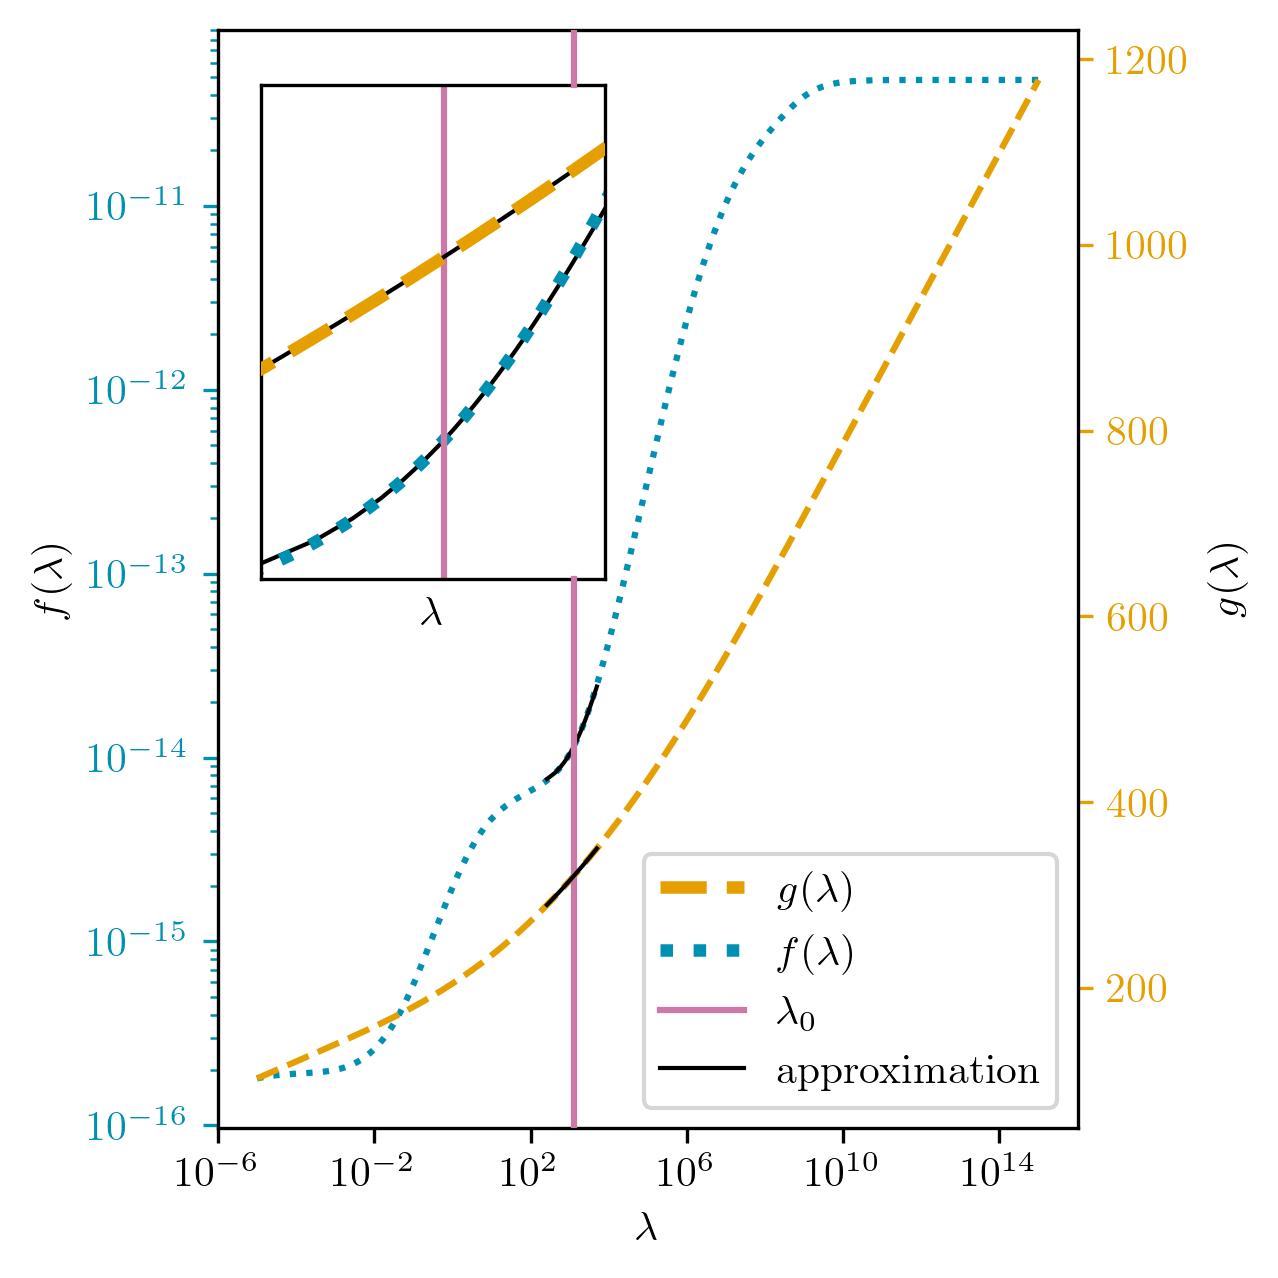
\includegraphics{f_and_g_phd.png}
	\caption[Plot of the functions $f(\lambda)$ and $g(\lambda)$ for marginal posterior.]{Plot of the functions $f(\lambda)$ and $g(\lambda)$ for marginal posterior for a wide range of $\lambda = \delta / \gamma$. We plot the third Taylor series expansion in black around the mode of the marginal posterior (vertical line) for the sampling range of $\lambda$ within the MTC scheme.}
	\label{fig:fandg}
\end{figure}

%\begin{figure}[ht!]
%	\centering
%	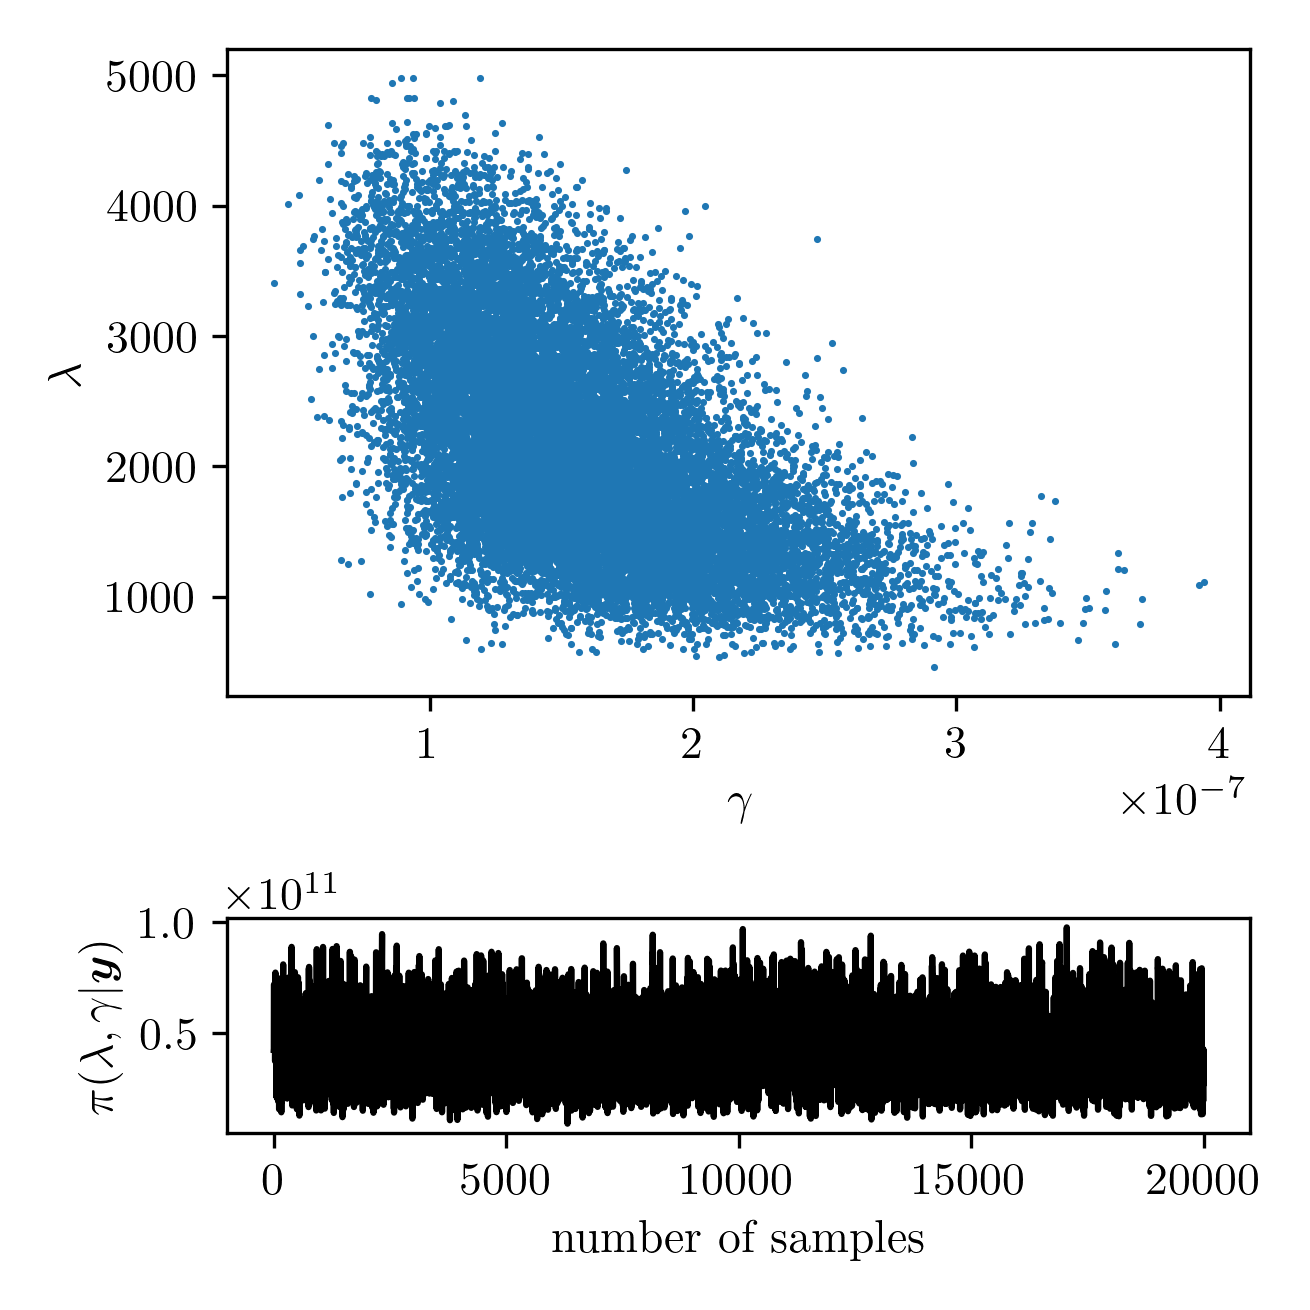
\includegraphics{ScatterplusHisto.png}
%	\caption[]{}
%	\label{fig:}
%\end{figure}

\begin{figure}[ht!]
	\centering
	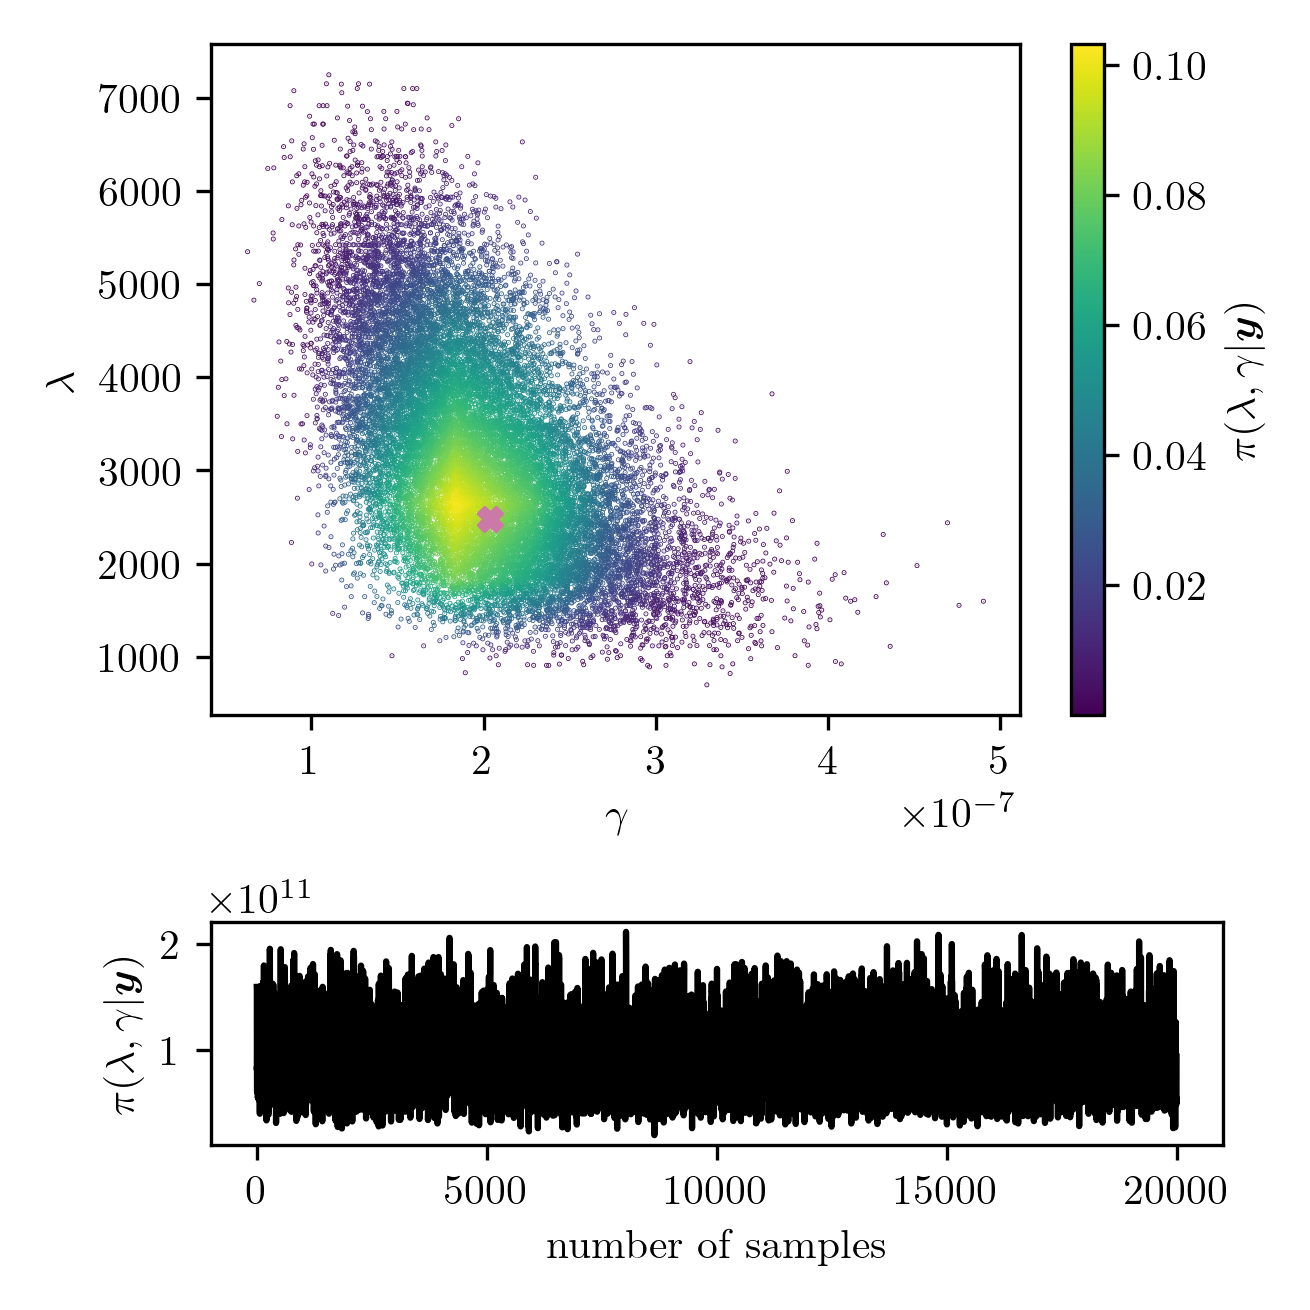
\includegraphics{ScatterplusHistoPlusTT.png}
	\caption[Scatter plot of samples from marginal posterior, including weighting from TT approximation; additional trace plot of the marginal posterior samples.]{We scatter plot the samples of $\lambda = \delta / \gamma $ and $\gamma$ from the marginal posterior $\pi(\lambda , \gamma  | \bm{y})$ and colour code the samples using the TT approximation of $\pi(\lambda , \gamma  | \bm{y})$. To show ergodicity we plot the trace of the samples of the Metropolis-within-Gibbs sampler below.}
	\label{fig:ScatterPlotTT}
\end{figure}


\subsubsection{sampling from conditional posterior Posterior}
\begin{itemize}
	\item draw samples using RTO no need to calc variance yet, when variance is hard to calculate, we use Cholesky defactorization (maybe put in appendix)
	\item or calc mean and variance using see other section
\end{itemize}
\begin{figure}[ht!]
	\centering
	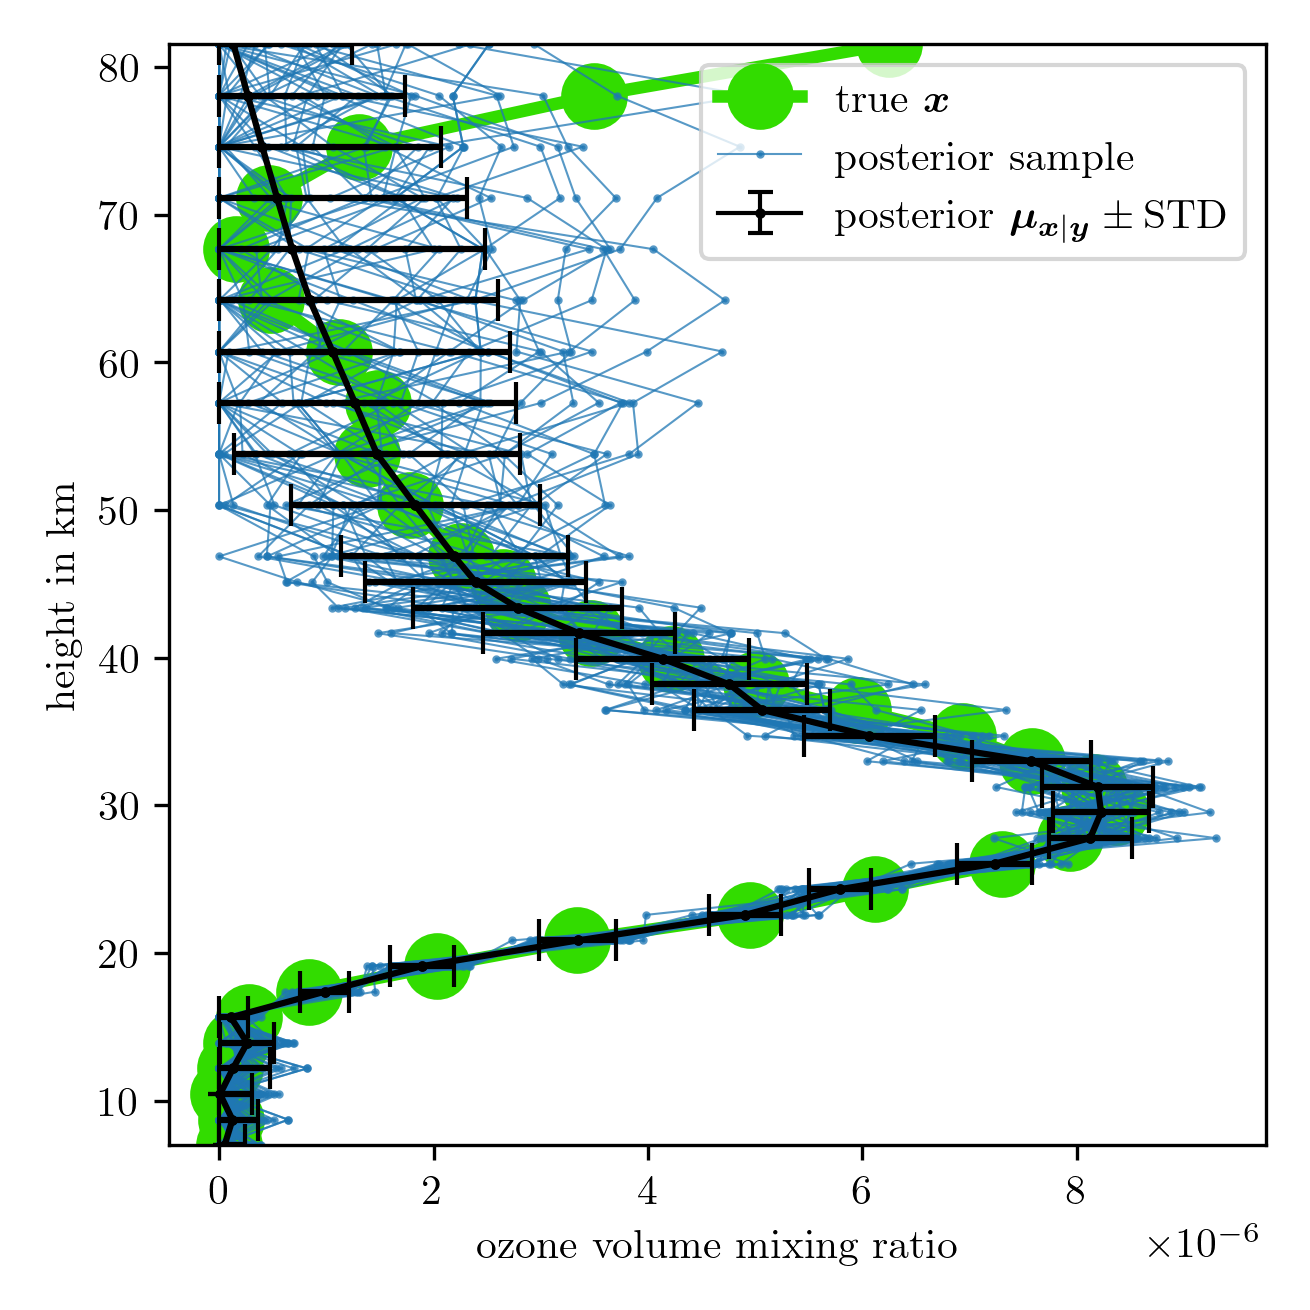
\includegraphics{FirstTestRes.png}
	\caption[Ozone samples of the conditional posterior.]{We draw samples from the conditional posterior distribution  $\pi(\bm{x}|\lambda,\gamma , \bm{y})$ after characterising the marginal posterior $\pi(\lambda,\gamma | \bm{y})$ through sampling or TT approximation using the linear forward map $\bm{A}_L$. We will use those samples to find the affine map $\bm{M}$, see section \ref{sec:affineMap}}
	\label{fig:O3Samp}
\end{figure}


\subsection{Generate and Asses Affine Map}
\begin{figure}[ht!]
	\centering
	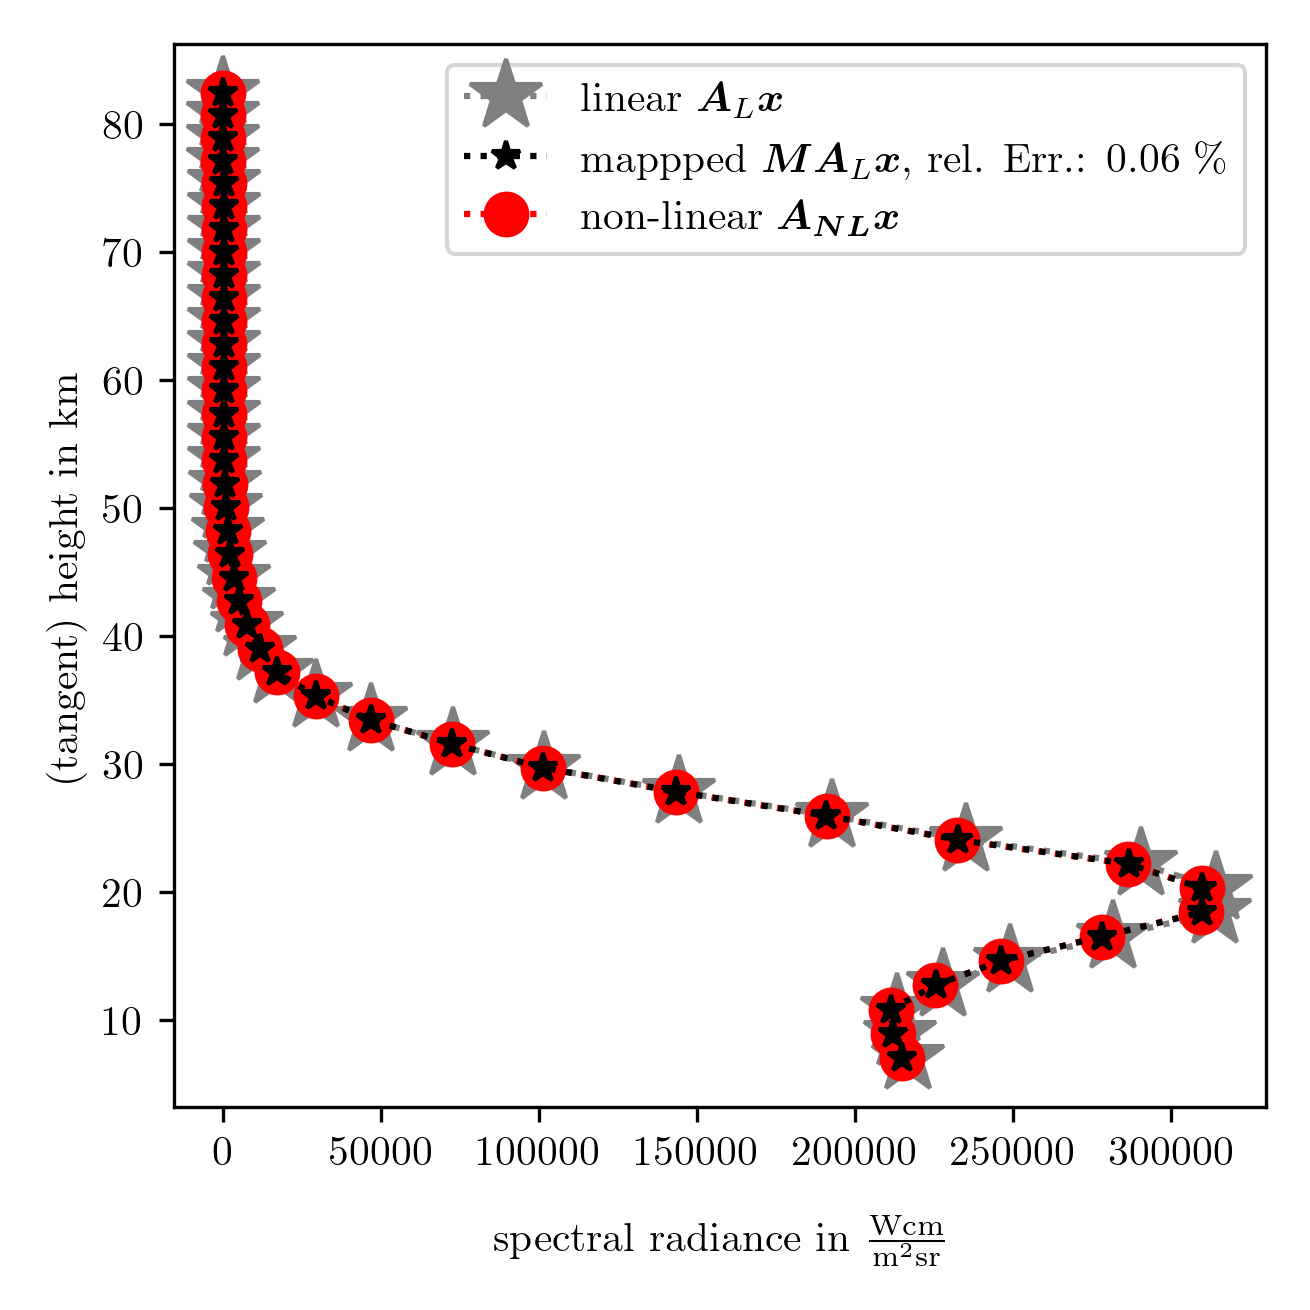
\includegraphics{SampMapAssesment.png}
	\caption[Assessment of affine map.]{We asses how good we can map the linear forward model onto the non-linear forward model using the previous calculated affine map. The gray stars represent noise free linear data, where as the red circles present noise free non-linear data. Then we map the linear noise free data onto the non-linear noise free data and give the relative error in between the mapped noise free data and the non-linear data. the  needs M}
	\label{fig:MapAsses}
\end{figure}


\section{Updated Forward map}

\begin{itemize}
	\item updated forward map
	\item do mtc again but this time with weighted integration and then condition on pressure and temperature, samples
	\item for sake of completeness regularised solution and say disadvantage, maybe include in table
\end{itemize}


\subsection{Ozone Retrieval}
%\begin{figure}[ht!]
%	\centering
%	\includegraphics{secRecRes.png}
%	\caption[]{}
%	\label{fig:}
%\end{figure}

\subsubsection{MTC --  sampling vs TT}
\begin{figure}[ht!]
	\centering
	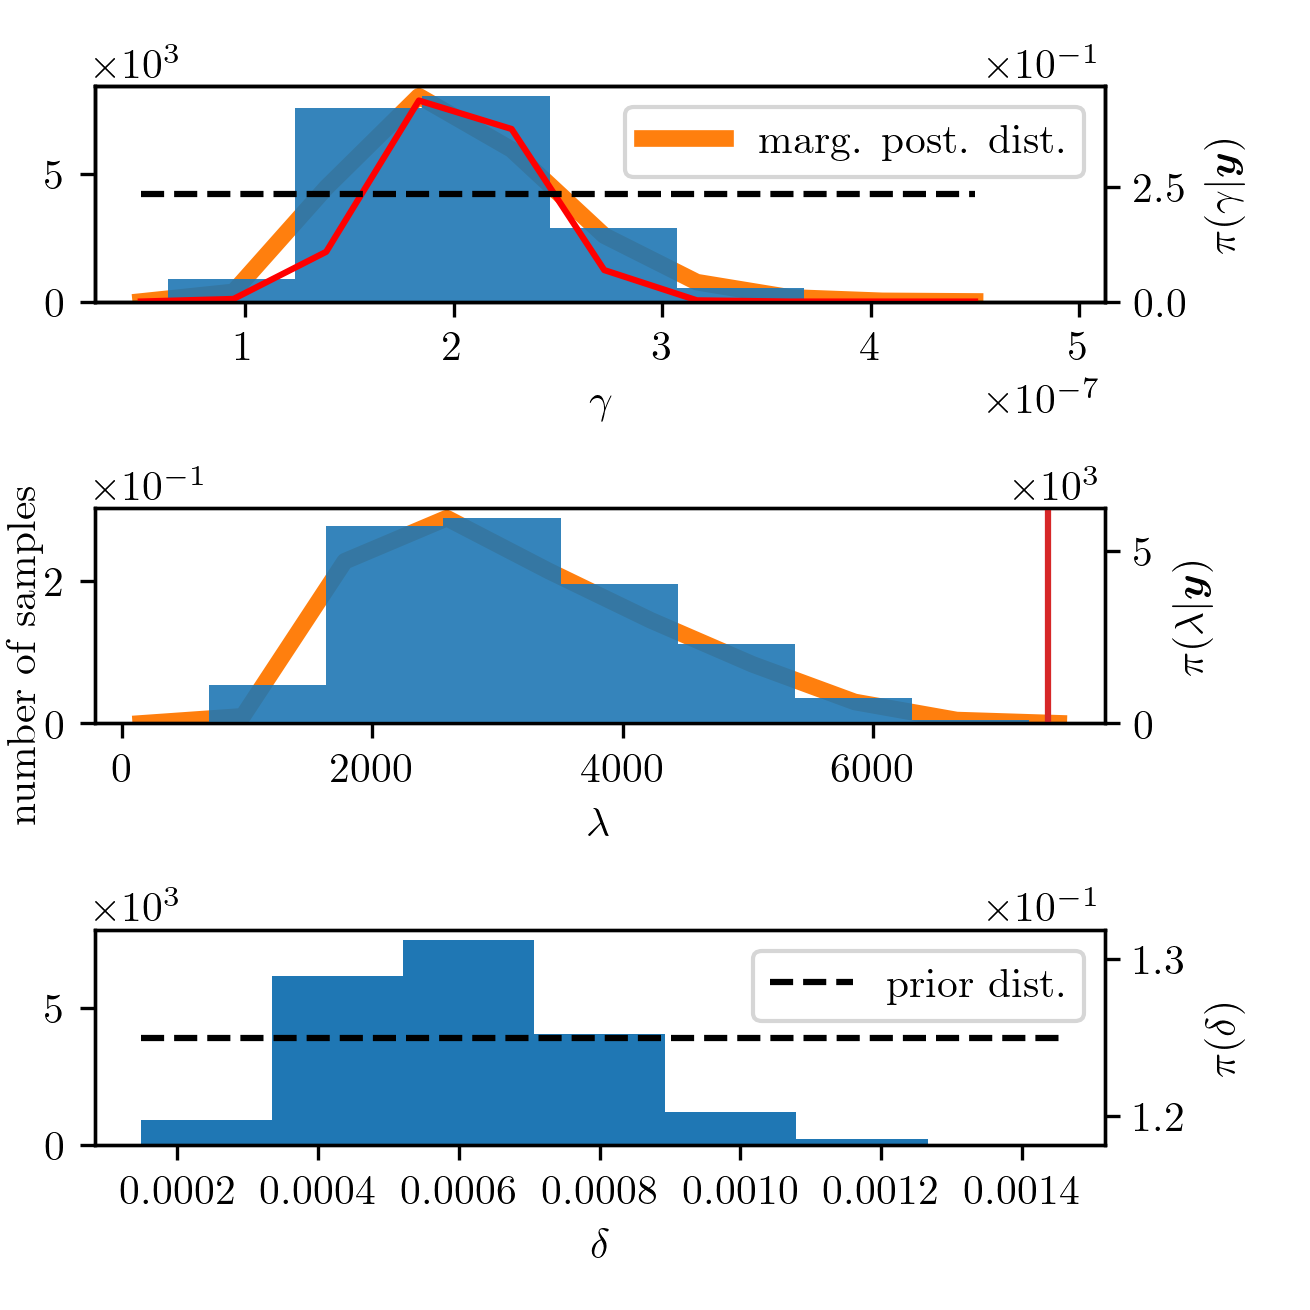
\includegraphics{secSIRTMargMargO3Res.png}
	\caption[Marginal posterior histograms and TT approximation as well as hyper-prior distribution.]{We plot the TT approximation of marginal posterior in orange and the samples as a histogram as well as the prior distribution with a dotted line. Note that we sample $\lambda$ and $\gamma$ using the Metropolis-within-Gibbs sampler and can calculate $\delta$ for every sample of the marginal posterior, we can not do this for the TT approximation. The regularised parameter corresponding to the regularised solution is marked thought the red vertical line at $\lambda_{\text{reg}} =$.}
	\label{fig:MargPostHistTT}
\end{figure}
\subsubsection{Regularized Solution}
\begin{itemize}
	\item similar to MTC model
	\item picture of L-Curve and samples 
	\item include in reg paraemter in histograms
\end{itemize}
\begin{figure}[ht!]
	\centering
	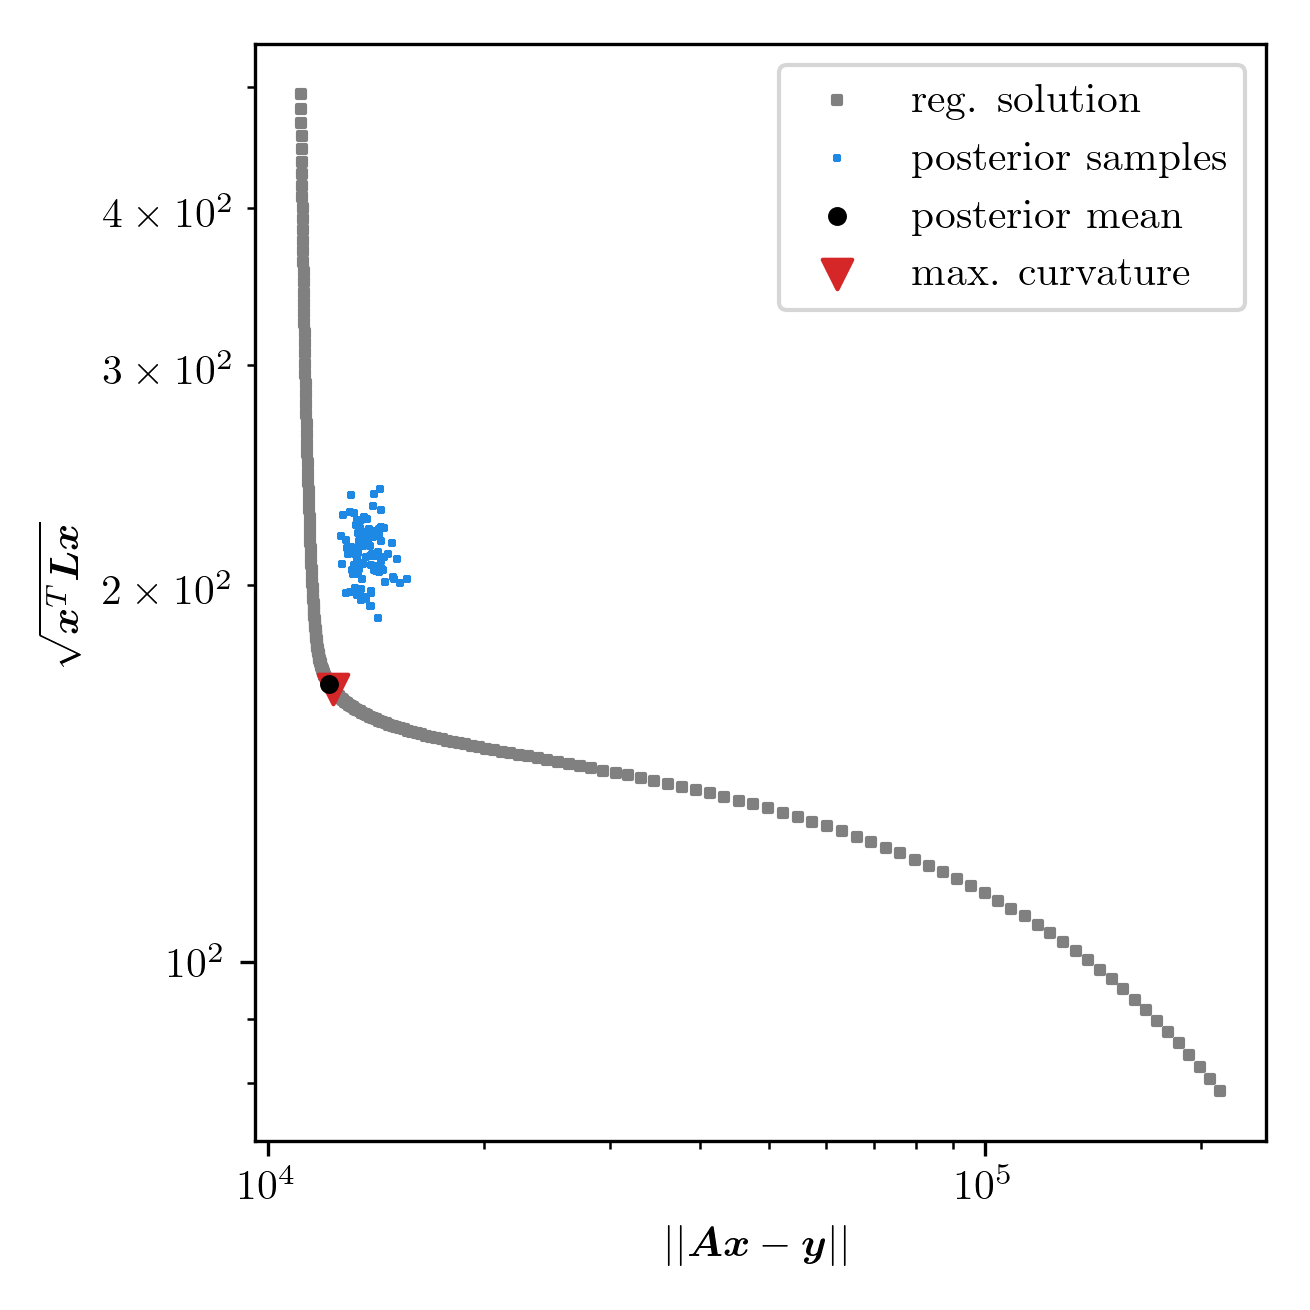
\includegraphics{LCurvePhD.png}
	\caption[Plot of the L-curve to find the regularised solution.]{We calculate regularised solution as in Eq. \ref{eq:} and plot the regularised semi norm $\sqrt{\bm{x}^T\bm{Lx}}$ against the data misfit norm $||\bm{Ax} -\bm{y} ||$ to find the regularised solution at the point of maximum curvature of the so-called L-Curve. Additionally we calculate the data misfit norm and the regularised norm for the ozone posterior and for samples of the conditional posterior distribution.}
	\label{fig:LCurve}
\end{figure}

\begin{figure}[ht!]
	\centering
	\includegraphics{SecRecResinclReg.png}
	\caption[Ozone posterior mean and variance and the regularised solution compared to the ground truth.]{We plot the conditional posterior mean and variance in black and the regularised solution on top of the ground truth ozone profile in green. We use the updated forward map $\bm{M}\bm{A}_L$}
	\label{fig:O3SolplsReg}
\end{figure}




\subsection{Posterior Pressure and Temperature}
\begin{itemize}
	\item make table with set up for TT and sampling t-walk
\end{itemize}
\begin{figure}[thb!]
	\centering
	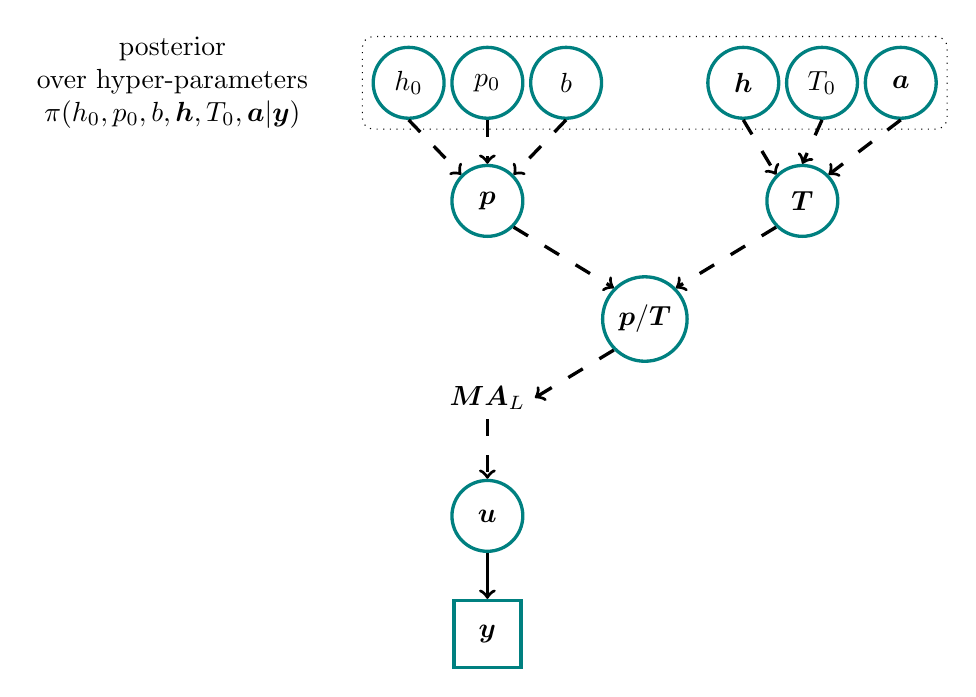
\begin{tikzpicture}
		
		\node[align=center] at (-1,4) (A)    {$\bm{M A}_L$};
		\node[roundnode2] at (-1,2.5) (u)    {$\bm{u}$};
		\node[rectnode] at (-1,1) (y)    {$\bm{y}$};
		
		\node[roundnode2] at (3,6.5) (t)     {$\bm{T}$};
		\node[roundnode2] at (-1,6.5) (p)     {$\bm{p}$};
		\node[roundnode2] at (1,5) (pt)     {$\bm{p}/\bm{T}$};
		\node[roundnode2] at (0,8) (b1)    {$b$};
		%\node[roundnode2] at (1,8) (b2)    {$b_2$};
		\node[roundnode2] at (-2,8) (h1)    {$h_0$};
		\node[roundnode2] at (-1,8) (p0)    {$p_0$};
		\node[roundnode2] at (2.25,8) (ht)    {$\bm{h}$};
		\node[roundnode2] at (3.25,8) (ct)    {$T_0$};
		\node[roundnode2] at (4.25,8) (at)    {$\bm{a}$};
		
		%Lines
		\draw[->, very thick] (u.south) -- (y.north);
		\draw[->, mydotted, very thick] (A.south) -- (u.north);
		
		\draw[->, mydotted, very thick] (p.south east) -- (pt.north west);
		\draw[->, mydotted, very thick] (t.south west) -- (pt.north east);
		\draw[->, mydotted, very thick] (pt.south west) -- (A.east);
		\draw[->, mydotted, very thick] (h1.south) -- (p.north west);
		\draw[->, mydotted, very thick] (p0.south) -- (p.north);
		\draw[->, mydotted, very thick] (b1.south) -- (p.north east); 
		%\draw[->, very thick] (b2.south) -- (p.east); 
		
		\draw[->, mydotted, very thick] (ht.south) -- (t.north west);
		\draw[->, mydotted, very thick] (ct.south) -- (t.north);
		\draw[->, mydotted, very thick] (at.south) -- (t.north east);
		
		\node[align =center] at (-5,8) (T1) {posterior \\ over hyper-parameters \\ $\pi(h_0, p_0, b, \bm{h}, T_0, \bm{a}| \bm{y})$};
		
		\node[fit=(h1)(at),draw,dotted,black, rounded corners] {};
	\end{tikzpicture} 
\caption[Directed acyclic Graph for pressure and temperature.]{Conditioned on an ozone profile the posterior of the hyper-parameters describing pressure and temperature is given as in Eq. \ref{eq:}. Since pressure and temperature go into the forward model as $\bm{p}/\bm{T}$ they are highly correlated but the pressure is the dominant parameter, see Fig. 
	\ref{fig:PriorPressOverTemp} and \ref{fig:SeaLevelHist}. Note that here we use the updated forward model $\bm{M} \bm{A}_L$ and conditioned on a $\gamma$ sample from the previously evaluated marginal posterior see Fig. \ref{fig:MargPostHistTT}. }
	\label{fig:DAGPT}
\end{figure}

\begin{figure}[ht!]
	\centering
	\includegraphics{PHdPTPost0.png}
	\caption[Histograms and TT approximation of posterior distribution as well as hyper-prior distribution.]{We plot the TT approximation of marginal posterior in orange and the samples as a histogram as well as the prior distribution with a dotted line.}
	\label{fig:PostHistTT0}
\end{figure}
\begin{figure}[ht!]
	\centering
	\includegraphics{PHdPTPost1.png}
	\caption[Histograms and TT approximation of posterior distribution as well as hyper-prior distribution.]{We plot the TT approximation of marginal posterior in orange and the samples as a histogram as well as the prior distribution with a dotted line.}
	\label{fig:PostHistTT1}
\end{figure}
\begin{figure}[ht!]
	\centering
	\includegraphics{PHdPTPost2.png}
	\caption[Histograms and TT approximation of posterior distribution as well as hyper-prior distribution.]{We plot the TT approximation of marginal posterior in orange and the samples as a histogram as well as the prior distribution with a dotted line.}
	\label{fig:PostHistTT2}
\end{figure}
\begin{figure}[ht!]
	\centering
	\includegraphics{PHdPTPost3.png}
	\caption[Histograms and TT approximation of posterior distribution as well as hyper-prior distribution.]{We plot the TT approximation of marginal posterior in orange and the samples as a histogram as well as the prior distribution with a dotted line.}
	\label{fig:PostHistTT3}
\end{figure}
\begin{figure}[ht!]
	\centering
	\includegraphics{PHdPTPost4.png}
	\caption[Histograms and TT approximation of posterior distribution as well as hyper-prior distribution.]{We plot the TT approximation of marginal posterior in orange and the samples as a histogram as well as the prior distribution with a dotted line.}
	\label{fig:PostHistTT4}
\end{figure}

\begin{figure}[ht!]
	\centering
	\includegraphics{TempPostMeanSigm.png}
	\caption[Temperature posterior samples.]{We take samples from the posterior distribution, as plotted in Figures \ref{fig:PostHistTT0} to \ref{fig:PostHistTT3} and plot the corresponding temperature function, see Eq: \ref{eq:tempFunc}. }
	\label{fig:TempPost}
\end{figure}

\begin{figure}[ht!]
	\centering
	\includegraphics{PressPostMeanSigm.png}
	\caption[Pressure posterior samples.]{We take samples from the posterior distribution, as plotted in Fig. \ref{fig:PostHistTT4} and plot the corresponding pressure function, see Eq: \ref{eq:pressFunc}.}
	\label{fig:PressPost}
\end{figure}



@misc{MLSdata,
	title= {MLS/Aura Level 2 Ozone (O3) Mixing Ratio V005},
	author = {Schwartz, M., Froidevaux, L., Livesey, N. and Read, W.},
	year = {2020},
	howpublished ={\url{https://disc.gsfc.nasa.gov/datasets/ML2O3_005/summary?keywords=mls%20o3}},
	publisher = {Goddard Earth Sciences Data and Information Services Center (GES DISC)},
	adress = {Greenbelt, MD, USA},
	note = "[Online; accessed 25/04/24, 10.5067/Aura/MLS/DATA2516]"
}



\chapter{Conclusion}

\begin{itemize}
	\item Data sensitive informative uninformative, Ozone in higher altitude, pressure , temperature
	\item SNR v s Pointing accuracy from experience
	\item include pointing accuracy, weighted mean for pointing accuracy
	\item Through exploratory analysis we found that instead of increasing the ranks optimising the tensors by sweeping over them gives better approximations and is faster, which is crucial in higher dimensions as in section \ref{sec:postPT}.
\end{itemize}
%
\chapter{Building a physics based hierarchical Linear model}
\begin{itemize}
	\item two hyperparameters, marginal and then conditonal, MTC, use as a building block \cite{fox2016fast, rue2005gaussian}
	\item  sampling, Gibbs-MH, t-walk \cite{christen2010general}
	\item increase hyperparameters, Temperature and pressure, tt-approx, SIRT \cite{cui2022deep, atmosphere1976us}
\end{itemize}

\begin{table}
	\centering
	\begin{tabular}{ |c||c|c|c|c|  }
		\hline
		\makecell{parameter\\ and context}& \makecell{$m$, number of\\ measurements}& \makecell{pointing\\ accuracy }& \makecell{$n$, number of \\atmospheric layers}& \makecell{signal-to-noise\\ voltage ratio}\\
		\hline
		$\bm{y}$, data& 33&  $0.009^{\circ}$ &43& 10\\
		\hline
	\end{tabular}
	\caption{Data Spec}
	\label{tab:}
\end{table}


\section{Linear model}
\begin{itemize}
	\item define model \cite{readings2000envisat}
	\item explain parameters and constants \cite{gordon2022hitran2020}
	\item how pressure to height and temperature hydro-static equilibrium equation \cite{atmosphere1976us}
\end{itemize}

\section{two hyperameters, fast sampling paper}
\begin{itemize}
	\item similar to MTC paper,  \cite{fox2016fast}
	\item can compare to regularization and can integrate easily with less solves to regularization or RTO, \cite{hansen1993use}
	\item define priors make table
	\item how many steps, integrated autocorrealtion time , ref
	\item relative error
	\item how I found max curvature, \cite{satopaa2011kneedle}
	\item how many taylor series
\end{itemize}

\begin{figure}[thb!]
	\centering
	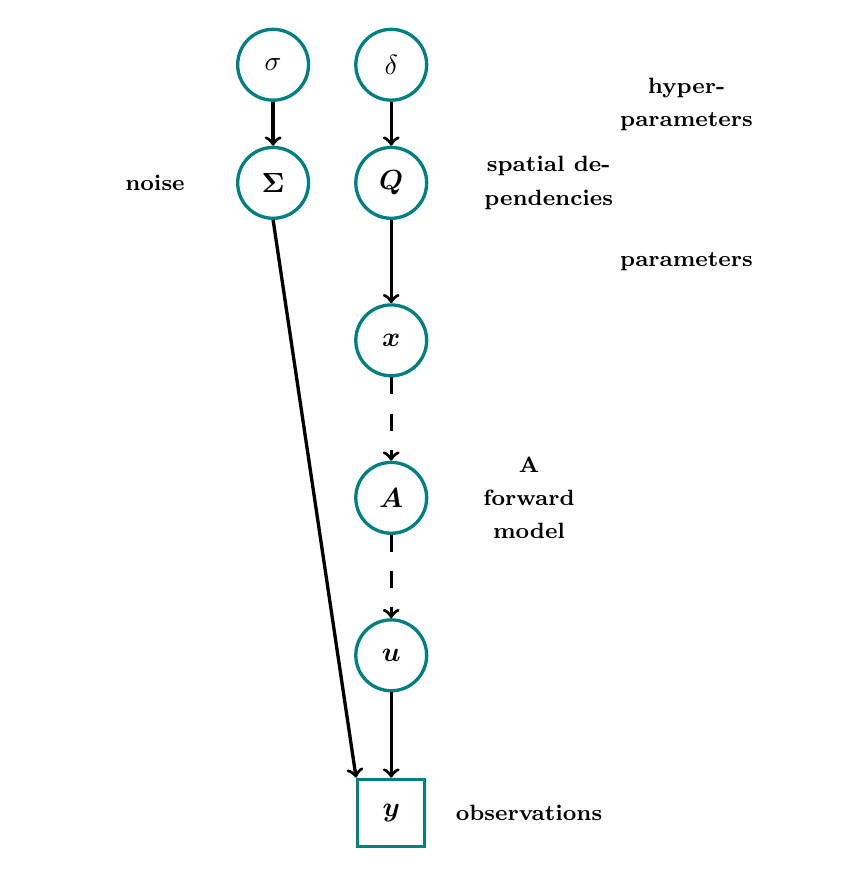
\begin{tikzpicture}
		\node[roundnode2] at (0,6) (Q)     {$\bm{Q}$};
		\node[roundnode2] at (0,4) (x)     {$\bm{x}$};
		\node[roundnode2] at (0,2) (A)    {$\bm{A}$};
		\node[roundnode2] at (0,0) (u)    {$\bm{u}$};
		\node[rectnode] at (0,-2) (y)    {$\bm{y}$};
		\node[roundnode2] at (-1.5,6) (S)    {$\bm{\Sigma}$};
		\node[roundnode2] at (-1.5,7.5) (s)    {$\sigma$};
		\node[roundnode2] at (0,7.5) (d)    {$\delta$};
		
		%text
		%\draw (-1,2.5) node[align=center, text width=1.5cm] {\footnotesize \textbf{hydrostatic \\ equation}};
		\draw (1.75,2) node[align=center, text width=1.5cm] {\footnotesize \textbf{A \\ forward model }};
		%\draw (6.75,-1.5) node[align=center, text width=2.5cm] {\footnotesize \textbf{hyper\-parameters}};
		%\draw (5.5,-1.5) node[align=center, text width=0.5cm] { $\bm{\theta}$};
		\draw (1.75,-2) node[align=center, text width=3cm] {\footnotesize \textbf{observations}};
		\draw (3.75,7) node[align=center, text width=3cm] {\footnotesize \textbf{hyper-\\parameters}};
		\draw (3.75,5) node[align=center, text width=3cm] {\footnotesize \textbf{parameters}};
		\draw (2,6) node[align=center, text width=3cm] {\footnotesize \textbf{spatial dependencies}};
		%\draw (-1.4,-2.3) node[align=center, text width=3cm] {\footnotesize \textbf{hyper-prior}};
		\draw (-3,6) node[align=center, text width=3cm] {\footnotesize \textbf{noise}};
		% Calligraphic brace
		%\draw[very thick, decorate,decoration = {brace}] (5,-1) --  (5,-2);
		
		%Lines
		\draw[->, very thick] (S.south) -- (y.north west);
		\draw[->, very thick] (s.south) -- (S.north);
		\draw[->, very thick] (u.south) -- (y.north);
		\draw[->, mydotted, very thick] (A.south) -- (u.north);
		\draw[->, mydotted,  very thick] (x.south) -- (A.north);
		
		\draw[->, very thick] (d.south) -- (Q.north); 
		\draw[->, very thick] (Q.south) -- (x.north); 
		
		
	\end{tikzpicture} 
	\caption[]{}
\end{figure}

\begin{figure}[!ht]
	\centering
	\renewcommand\sffamily{}
	\renewcommand{\mathbf}{\bm}
	%\includegraphics[width = 0.99\columnwidth]{f_and_g_paper.png}
	\scalebox{0.66}{\input{f_and_g_paper.pdf_tex}}
	%\input{f_and_g_paper.pdf_tex}
	\caption{Functions $f(\lambda)$, dotted, and $g(\lambda)$, dashed, of the marginal posterior distribution for the specific forward model used in this study. Both functions are well-behaved over a large range of $\lambda$. In the support region of the MWG the pink square refers to the mode of the marginal posterior. Additionally, we plot the Taylor series of fourth order for $f(\lambda)$ and $g(\lambda)$ around the mode, see black line.}
	\label{fig:f_and_g}
\end{figure}

\begin{figure}[!ht]
	\centering
	\renewcommand\sffamily{}
	\renewcommand{\mathbf}{\bm}
	%\scalebox{0.66}{\input{AllHistoResults.pgf}}
	\scalebox{0.66}{%% Creator: Matplotlib, PGF backend
%%
%% To include the figure in your LaTeX document, write
%%   \input{<filename>.pgf}
%%
%% Make sure the required packages are loaded in your preamble
%%   \usepackage{pgf}
%%
%% Also ensure that all the required font packages are loaded; for instance,
%% the lmodern package is sometimes necessary when using math font.
%%   \usepackage{lmodern}
%%
%% Figures using additional raster images can only be included by \input if
%% they are in the same directory as the main LaTeX file. For loading figures
%% from other directories you can use the `import` package
%%   \usepackage{import}
%%
%% and then include the figures with
%%   \import{<path to file>}{<filename>.pgf}
%%
%% Matplotlib used the following preamble
%%   
%%   \makeatletter\@ifpackageloaded{underscore}{}{\usepackage[strings]{underscore}}\makeatother
%%
\begingroup%
\makeatletter%
\begin{pgfpicture}%
\pgfpathrectangle{\pgfpointorigin}{\pgfqpoint{4.920000in}{4.920000in}}%
\pgfusepath{use as bounding box, clip}%
\begin{pgfscope}%
\pgfsetbuttcap%
\pgfsetmiterjoin%
\definecolor{currentfill}{rgb}{1.000000,1.000000,1.000000}%
\pgfsetfillcolor{currentfill}%
\pgfsetlinewidth{0.000000pt}%
\definecolor{currentstroke}{rgb}{1.000000,1.000000,1.000000}%
\pgfsetstrokecolor{currentstroke}%
\pgfsetdash{}{0pt}%
\pgfpathmoveto{\pgfqpoint{0.000000in}{0.000000in}}%
\pgfpathlineto{\pgfqpoint{4.920000in}{0.000000in}}%
\pgfpathlineto{\pgfqpoint{4.920000in}{4.920000in}}%
\pgfpathlineto{\pgfqpoint{0.000000in}{4.920000in}}%
\pgfpathlineto{\pgfqpoint{0.000000in}{0.000000in}}%
\pgfpathclose%
\pgfusepath{fill}%
\end{pgfscope}%
\begin{pgfscope}%
\pgfsetbuttcap%
\pgfsetmiterjoin%
\definecolor{currentfill}{rgb}{1.000000,1.000000,1.000000}%
\pgfsetfillcolor{currentfill}%
\pgfsetlinewidth{0.000000pt}%
\definecolor{currentstroke}{rgb}{0.000000,0.000000,0.000000}%
\pgfsetstrokecolor{currentstroke}%
\pgfsetstrokeopacity{0.000000}%
\pgfsetdash{}{0pt}%
\pgfpathmoveto{\pgfqpoint{0.854238in}{2.092082in}}%
\pgfpathlineto{\pgfqpoint{4.820000in}{2.092082in}}%
\pgfpathlineto{\pgfqpoint{4.820000in}{4.820000in}}%
\pgfpathlineto{\pgfqpoint{0.854238in}{4.820000in}}%
\pgfpathlineto{\pgfqpoint{0.854238in}{2.092082in}}%
\pgfpathclose%
\pgfusepath{fill}%
\end{pgfscope}%
\begin{pgfscope}%
\pgfpathrectangle{\pgfqpoint{0.854238in}{2.092082in}}{\pgfqpoint{3.965762in}{2.727918in}}%
\pgfusepath{clip}%
\pgfsetbuttcap%
\pgfsetroundjoin%
\definecolor{currentfill}{rgb}{0.000000,0.000000,0.000000}%
\pgfsetfillcolor{currentfill}%
\pgfsetlinewidth{1.003750pt}%
\definecolor{currentstroke}{rgb}{0.000000,0.000000,0.000000}%
\pgfsetstrokecolor{currentstroke}%
\pgfsetdash{}{0pt}%
\pgfsys@defobject{currentmarker}{\pgfqpoint{-0.020833in}{-0.020833in}}{\pgfqpoint{0.020833in}{0.020833in}}{%
\pgfpathmoveto{\pgfqpoint{0.000000in}{-0.020833in}}%
\pgfpathcurveto{\pgfqpoint{0.005525in}{-0.020833in}}{\pgfqpoint{0.010825in}{-0.018638in}}{\pgfqpoint{0.014731in}{-0.014731in}}%
\pgfpathcurveto{\pgfqpoint{0.018638in}{-0.010825in}}{\pgfqpoint{0.020833in}{-0.005525in}}{\pgfqpoint{0.020833in}{0.000000in}}%
\pgfpathcurveto{\pgfqpoint{0.020833in}{0.005525in}}{\pgfqpoint{0.018638in}{0.010825in}}{\pgfqpoint{0.014731in}{0.014731in}}%
\pgfpathcurveto{\pgfqpoint{0.010825in}{0.018638in}}{\pgfqpoint{0.005525in}{0.020833in}}{\pgfqpoint{0.000000in}{0.020833in}}%
\pgfpathcurveto{\pgfqpoint{-0.005525in}{0.020833in}}{\pgfqpoint{-0.010825in}{0.018638in}}{\pgfqpoint{-0.014731in}{0.014731in}}%
\pgfpathcurveto{\pgfqpoint{-0.018638in}{0.010825in}}{\pgfqpoint{-0.020833in}{0.005525in}}{\pgfqpoint{-0.020833in}{0.000000in}}%
\pgfpathcurveto{\pgfqpoint{-0.020833in}{-0.005525in}}{\pgfqpoint{-0.018638in}{-0.010825in}}{\pgfqpoint{-0.014731in}{-0.014731in}}%
\pgfpathcurveto{\pgfqpoint{-0.010825in}{-0.018638in}}{\pgfqpoint{-0.005525in}{-0.020833in}}{\pgfqpoint{0.000000in}{-0.020833in}}%
\pgfpathlineto{\pgfqpoint{0.000000in}{-0.020833in}}%
\pgfpathclose%
\pgfusepath{stroke,fill}%
}%
\begin{pgfscope}%
\pgfsys@transformshift{2.043625in}{3.407497in}%
\pgfsys@useobject{currentmarker}{}%
\end{pgfscope}%
\begin{pgfscope}%
\pgfsys@transformshift{2.119751in}{3.269421in}%
\pgfsys@useobject{currentmarker}{}%
\end{pgfscope}%
\begin{pgfscope}%
\pgfsys@transformshift{1.707597in}{3.049194in}%
\pgfsys@useobject{currentmarker}{}%
\end{pgfscope}%
\begin{pgfscope}%
\pgfsys@transformshift{1.836575in}{3.246105in}%
\pgfsys@useobject{currentmarker}{}%
\end{pgfscope}%
\begin{pgfscope}%
\pgfsys@transformshift{2.290375in}{3.179193in}%
\pgfsys@useobject{currentmarker}{}%
\end{pgfscope}%
\begin{pgfscope}%
\pgfsys@transformshift{2.735692in}{3.183461in}%
\pgfsys@useobject{currentmarker}{}%
\end{pgfscope}%
\begin{pgfscope}%
\pgfsys@transformshift{2.566950in}{4.142220in}%
\pgfsys@useobject{currentmarker}{}%
\end{pgfscope}%
\begin{pgfscope}%
\pgfsys@transformshift{2.341331in}{2.929143in}%
\pgfsys@useobject{currentmarker}{}%
\end{pgfscope}%
\begin{pgfscope}%
\pgfsys@transformshift{3.158086in}{3.249298in}%
\pgfsys@useobject{currentmarker}{}%
\end{pgfscope}%
\begin{pgfscope}%
\pgfsys@transformshift{2.889926in}{3.079613in}%
\pgfsys@useobject{currentmarker}{}%
\end{pgfscope}%
\begin{pgfscope}%
\pgfsys@transformshift{1.380199in}{3.041342in}%
\pgfsys@useobject{currentmarker}{}%
\end{pgfscope}%
\begin{pgfscope}%
\pgfsys@transformshift{2.239076in}{3.570717in}%
\pgfsys@useobject{currentmarker}{}%
\end{pgfscope}%
\begin{pgfscope}%
\pgfsys@transformshift{2.191076in}{2.885952in}%
\pgfsys@useobject{currentmarker}{}%
\end{pgfscope}%
\begin{pgfscope}%
\pgfsys@transformshift{1.484597in}{3.796933in}%
\pgfsys@useobject{currentmarker}{}%
\end{pgfscope}%
\begin{pgfscope}%
\pgfsys@transformshift{1.845087in}{3.864137in}%
\pgfsys@useobject{currentmarker}{}%
\end{pgfscope}%
\begin{pgfscope}%
\pgfsys@transformshift{1.705888in}{2.807564in}%
\pgfsys@useobject{currentmarker}{}%
\end{pgfscope}%
\begin{pgfscope}%
\pgfsys@transformshift{2.399218in}{4.333028in}%
\pgfsys@useobject{currentmarker}{}%
\end{pgfscope}%
\begin{pgfscope}%
\pgfsys@transformshift{2.390499in}{3.708101in}%
\pgfsys@useobject{currentmarker}{}%
\end{pgfscope}%
\begin{pgfscope}%
\pgfsys@transformshift{1.659209in}{3.317853in}%
\pgfsys@useobject{currentmarker}{}%
\end{pgfscope}%
\begin{pgfscope}%
\pgfsys@transformshift{2.282336in}{3.159560in}%
\pgfsys@useobject{currentmarker}{}%
\end{pgfscope}%
\begin{pgfscope}%
\pgfsys@transformshift{1.865595in}{3.082888in}%
\pgfsys@useobject{currentmarker}{}%
\end{pgfscope}%
\begin{pgfscope}%
\pgfsys@transformshift{2.559741in}{3.364065in}%
\pgfsys@useobject{currentmarker}{}%
\end{pgfscope}%
\begin{pgfscope}%
\pgfsys@transformshift{2.627812in}{3.414607in}%
\pgfsys@useobject{currentmarker}{}%
\end{pgfscope}%
\begin{pgfscope}%
\pgfsys@transformshift{2.252661in}{2.779246in}%
\pgfsys@useobject{currentmarker}{}%
\end{pgfscope}%
\begin{pgfscope}%
\pgfsys@transformshift{2.465137in}{3.204093in}%
\pgfsys@useobject{currentmarker}{}%
\end{pgfscope}%
\begin{pgfscope}%
\pgfsys@transformshift{1.735209in}{3.578415in}%
\pgfsys@useobject{currentmarker}{}%
\end{pgfscope}%
\begin{pgfscope}%
\pgfsys@transformshift{1.516331in}{3.561104in}%
\pgfsys@useobject{currentmarker}{}%
\end{pgfscope}%
\begin{pgfscope}%
\pgfsys@transformshift{2.489923in}{3.300069in}%
\pgfsys@useobject{currentmarker}{}%
\end{pgfscope}%
\begin{pgfscope}%
\pgfsys@transformshift{2.530425in}{3.552916in}%
\pgfsys@useobject{currentmarker}{}%
\end{pgfscope}%
\begin{pgfscope}%
\pgfsys@transformshift{2.831219in}{3.647331in}%
\pgfsys@useobject{currentmarker}{}%
\end{pgfscope}%
\begin{pgfscope}%
\pgfsys@transformshift{2.609308in}{3.264935in}%
\pgfsys@useobject{currentmarker}{}%
\end{pgfscope}%
\begin{pgfscope}%
\pgfsys@transformshift{2.485345in}{3.122114in}%
\pgfsys@useobject{currentmarker}{}%
\end{pgfscope}%
\begin{pgfscope}%
\pgfsys@transformshift{2.731362in}{3.353346in}%
\pgfsys@useobject{currentmarker}{}%
\end{pgfscope}%
\begin{pgfscope}%
\pgfsys@transformshift{2.769397in}{3.504885in}%
\pgfsys@useobject{currentmarker}{}%
\end{pgfscope}%
\begin{pgfscope}%
\pgfsys@transformshift{1.987129in}{3.674076in}%
\pgfsys@useobject{currentmarker}{}%
\end{pgfscope}%
\begin{pgfscope}%
\pgfsys@transformshift{2.036893in}{2.702229in}%
\pgfsys@useobject{currentmarker}{}%
\end{pgfscope}%
\begin{pgfscope}%
\pgfsys@transformshift{2.296886in}{3.323460in}%
\pgfsys@useobject{currentmarker}{}%
\end{pgfscope}%
\begin{pgfscope}%
\pgfsys@transformshift{3.369148in}{2.830219in}%
\pgfsys@useobject{currentmarker}{}%
\end{pgfscope}%
\begin{pgfscope}%
\pgfsys@transformshift{2.290682in}{2.957613in}%
\pgfsys@useobject{currentmarker}{}%
\end{pgfscope}%
\begin{pgfscope}%
\pgfsys@transformshift{1.646551in}{4.131457in}%
\pgfsys@useobject{currentmarker}{}%
\end{pgfscope}%
\begin{pgfscope}%
\pgfsys@transformshift{1.683503in}{2.846457in}%
\pgfsys@useobject{currentmarker}{}%
\end{pgfscope}%
\begin{pgfscope}%
\pgfsys@transformshift{2.310535in}{3.037404in}%
\pgfsys@useobject{currentmarker}{}%
\end{pgfscope}%
\begin{pgfscope}%
\pgfsys@transformshift{2.067139in}{3.268506in}%
\pgfsys@useobject{currentmarker}{}%
\end{pgfscope}%
\begin{pgfscope}%
\pgfsys@transformshift{2.621473in}{3.088569in}%
\pgfsys@useobject{currentmarker}{}%
\end{pgfscope}%
\begin{pgfscope}%
\pgfsys@transformshift{2.930515in}{3.216203in}%
\pgfsys@useobject{currentmarker}{}%
\end{pgfscope}%
\begin{pgfscope}%
\pgfsys@transformshift{1.288864in}{3.029120in}%
\pgfsys@useobject{currentmarker}{}%
\end{pgfscope}%
\begin{pgfscope}%
\pgfsys@transformshift{2.195155in}{3.783760in}%
\pgfsys@useobject{currentmarker}{}%
\end{pgfscope}%
\begin{pgfscope}%
\pgfsys@transformshift{2.762095in}{3.546178in}%
\pgfsys@useobject{currentmarker}{}%
\end{pgfscope}%
\begin{pgfscope}%
\pgfsys@transformshift{2.796273in}{3.080077in}%
\pgfsys@useobject{currentmarker}{}%
\end{pgfscope}%
\begin{pgfscope}%
\pgfsys@transformshift{2.485281in}{4.510916in}%
\pgfsys@useobject{currentmarker}{}%
\end{pgfscope}%
\begin{pgfscope}%
\pgfsys@transformshift{1.613229in}{2.633496in}%
\pgfsys@useobject{currentmarker}{}%
\end{pgfscope}%
\begin{pgfscope}%
\pgfsys@transformshift{2.581159in}{3.388983in}%
\pgfsys@useobject{currentmarker}{}%
\end{pgfscope}%
\begin{pgfscope}%
\pgfsys@transformshift{2.360751in}{3.006697in}%
\pgfsys@useobject{currentmarker}{}%
\end{pgfscope}%
\begin{pgfscope}%
\pgfsys@transformshift{1.954994in}{3.343699in}%
\pgfsys@useobject{currentmarker}{}%
\end{pgfscope}%
\begin{pgfscope}%
\pgfsys@transformshift{3.141239in}{3.709168in}%
\pgfsys@useobject{currentmarker}{}%
\end{pgfscope}%
\begin{pgfscope}%
\pgfsys@transformshift{2.970675in}{3.309702in}%
\pgfsys@useobject{currentmarker}{}%
\end{pgfscope}%
\begin{pgfscope}%
\pgfsys@transformshift{2.585361in}{3.081317in}%
\pgfsys@useobject{currentmarker}{}%
\end{pgfscope}%
\begin{pgfscope}%
\pgfsys@transformshift{1.741575in}{4.071216in}%
\pgfsys@useobject{currentmarker}{}%
\end{pgfscope}%
\begin{pgfscope}%
\pgfsys@transformshift{1.790316in}{3.055721in}%
\pgfsys@useobject{currentmarker}{}%
\end{pgfscope}%
\begin{pgfscope}%
\pgfsys@transformshift{1.591922in}{2.911854in}%
\pgfsys@useobject{currentmarker}{}%
\end{pgfscope}%
\begin{pgfscope}%
\pgfsys@transformshift{1.760695in}{3.584190in}%
\pgfsys@useobject{currentmarker}{}%
\end{pgfscope}%
\begin{pgfscope}%
\pgfsys@transformshift{2.283656in}{3.668231in}%
\pgfsys@useobject{currentmarker}{}%
\end{pgfscope}%
\begin{pgfscope}%
\pgfsys@transformshift{1.961119in}{4.045434in}%
\pgfsys@useobject{currentmarker}{}%
\end{pgfscope}%
\begin{pgfscope}%
\pgfsys@transformshift{2.759996in}{3.258569in}%
\pgfsys@useobject{currentmarker}{}%
\end{pgfscope}%
\begin{pgfscope}%
\pgfsys@transformshift{1.489189in}{3.198395in}%
\pgfsys@useobject{currentmarker}{}%
\end{pgfscope}%
\begin{pgfscope}%
\pgfsys@transformshift{2.602335in}{3.321794in}%
\pgfsys@useobject{currentmarker}{}%
\end{pgfscope}%
\begin{pgfscope}%
\pgfsys@transformshift{2.189678in}{3.308873in}%
\pgfsys@useobject{currentmarker}{}%
\end{pgfscope}%
\begin{pgfscope}%
\pgfsys@transformshift{2.455038in}{3.983515in}%
\pgfsys@useobject{currentmarker}{}%
\end{pgfscope}%
\begin{pgfscope}%
\pgfsys@transformshift{2.143125in}{3.187013in}%
\pgfsys@useobject{currentmarker}{}%
\end{pgfscope}%
\begin{pgfscope}%
\pgfsys@transformshift{2.341635in}{2.989514in}%
\pgfsys@useobject{currentmarker}{}%
\end{pgfscope}%
\begin{pgfscope}%
\pgfsys@transformshift{1.912998in}{3.788686in}%
\pgfsys@useobject{currentmarker}{}%
\end{pgfscope}%
\begin{pgfscope}%
\pgfsys@transformshift{1.858034in}{3.853805in}%
\pgfsys@useobject{currentmarker}{}%
\end{pgfscope}%
\begin{pgfscope}%
\pgfsys@transformshift{1.279687in}{3.146293in}%
\pgfsys@useobject{currentmarker}{}%
\end{pgfscope}%
\begin{pgfscope}%
\pgfsys@transformshift{1.914353in}{3.144664in}%
\pgfsys@useobject{currentmarker}{}%
\end{pgfscope}%
\begin{pgfscope}%
\pgfsys@transformshift{2.290631in}{3.228443in}%
\pgfsys@useobject{currentmarker}{}%
\end{pgfscope}%
\begin{pgfscope}%
\pgfsys@transformshift{2.109041in}{2.854416in}%
\pgfsys@useobject{currentmarker}{}%
\end{pgfscope}%
\begin{pgfscope}%
\pgfsys@transformshift{2.190986in}{3.247594in}%
\pgfsys@useobject{currentmarker}{}%
\end{pgfscope}%
\begin{pgfscope}%
\pgfsys@transformshift{1.589699in}{3.240683in}%
\pgfsys@useobject{currentmarker}{}%
\end{pgfscope}%
\begin{pgfscope}%
\pgfsys@transformshift{1.969123in}{3.018591in}%
\pgfsys@useobject{currentmarker}{}%
\end{pgfscope}%
\begin{pgfscope}%
\pgfsys@transformshift{2.520378in}{3.355702in}%
\pgfsys@useobject{currentmarker}{}%
\end{pgfscope}%
\begin{pgfscope}%
\pgfsys@transformshift{2.463160in}{3.335061in}%
\pgfsys@useobject{currentmarker}{}%
\end{pgfscope}%
\begin{pgfscope}%
\pgfsys@transformshift{2.082641in}{3.641560in}%
\pgfsys@useobject{currentmarker}{}%
\end{pgfscope}%
\begin{pgfscope}%
\pgfsys@transformshift{2.049091in}{3.214446in}%
\pgfsys@useobject{currentmarker}{}%
\end{pgfscope}%
\begin{pgfscope}%
\pgfsys@transformshift{2.001095in}{3.462845in}%
\pgfsys@useobject{currentmarker}{}%
\end{pgfscope}%
\begin{pgfscope}%
\pgfsys@transformshift{2.110193in}{3.758457in}%
\pgfsys@useobject{currentmarker}{}%
\end{pgfscope}%
\begin{pgfscope}%
\pgfsys@transformshift{2.446627in}{3.107903in}%
\pgfsys@useobject{currentmarker}{}%
\end{pgfscope}%
\begin{pgfscope}%
\pgfsys@transformshift{2.620706in}{3.036273in}%
\pgfsys@useobject{currentmarker}{}%
\end{pgfscope}%
\begin{pgfscope}%
\pgfsys@transformshift{3.179779in}{2.697846in}%
\pgfsys@useobject{currentmarker}{}%
\end{pgfscope}%
\begin{pgfscope}%
\pgfsys@transformshift{1.604764in}{2.975547in}%
\pgfsys@useobject{currentmarker}{}%
\end{pgfscope}%
\begin{pgfscope}%
\pgfsys@transformshift{2.271144in}{3.260315in}%
\pgfsys@useobject{currentmarker}{}%
\end{pgfscope}%
\begin{pgfscope}%
\pgfsys@transformshift{1.787135in}{2.820968in}%
\pgfsys@useobject{currentmarker}{}%
\end{pgfscope}%
\begin{pgfscope}%
\pgfsys@transformshift{2.871577in}{2.641681in}%
\pgfsys@useobject{currentmarker}{}%
\end{pgfscope}%
\begin{pgfscope}%
\pgfsys@transformshift{2.368881in}{2.877963in}%
\pgfsys@useobject{currentmarker}{}%
\end{pgfscope}%
\begin{pgfscope}%
\pgfsys@transformshift{3.039115in}{3.116475in}%
\pgfsys@useobject{currentmarker}{}%
\end{pgfscope}%
\begin{pgfscope}%
\pgfsys@transformshift{3.292306in}{3.502830in}%
\pgfsys@useobject{currentmarker}{}%
\end{pgfscope}%
\begin{pgfscope}%
\pgfsys@transformshift{3.159958in}{3.080947in}%
\pgfsys@useobject{currentmarker}{}%
\end{pgfscope}%
\begin{pgfscope}%
\pgfsys@transformshift{1.774457in}{3.075341in}%
\pgfsys@useobject{currentmarker}{}%
\end{pgfscope}%
\begin{pgfscope}%
\pgfsys@transformshift{2.288229in}{3.597778in}%
\pgfsys@useobject{currentmarker}{}%
\end{pgfscope}%
\begin{pgfscope}%
\pgfsys@transformshift{2.028509in}{3.283525in}%
\pgfsys@useobject{currentmarker}{}%
\end{pgfscope}%
\begin{pgfscope}%
\pgfsys@transformshift{2.559880in}{2.892216in}%
\pgfsys@useobject{currentmarker}{}%
\end{pgfscope}%
\begin{pgfscope}%
\pgfsys@transformshift{1.813550in}{3.160206in}%
\pgfsys@useobject{currentmarker}{}%
\end{pgfscope}%
\begin{pgfscope}%
\pgfsys@transformshift{1.918006in}{3.133886in}%
\pgfsys@useobject{currentmarker}{}%
\end{pgfscope}%
\begin{pgfscope}%
\pgfsys@transformshift{3.556324in}{2.572097in}%
\pgfsys@useobject{currentmarker}{}%
\end{pgfscope}%
\begin{pgfscope}%
\pgfsys@transformshift{1.770643in}{3.907349in}%
\pgfsys@useobject{currentmarker}{}%
\end{pgfscope}%
\begin{pgfscope}%
\pgfsys@transformshift{2.422310in}{3.818535in}%
\pgfsys@useobject{currentmarker}{}%
\end{pgfscope}%
\begin{pgfscope}%
\pgfsys@transformshift{2.019449in}{3.445042in}%
\pgfsys@useobject{currentmarker}{}%
\end{pgfscope}%
\begin{pgfscope}%
\pgfsys@transformshift{2.899289in}{3.626831in}%
\pgfsys@useobject{currentmarker}{}%
\end{pgfscope}%
\begin{pgfscope}%
\pgfsys@transformshift{2.126218in}{3.083108in}%
\pgfsys@useobject{currentmarker}{}%
\end{pgfscope}%
\begin{pgfscope}%
\pgfsys@transformshift{2.076971in}{3.360509in}%
\pgfsys@useobject{currentmarker}{}%
\end{pgfscope}%
\begin{pgfscope}%
\pgfsys@transformshift{1.554324in}{3.500860in}%
\pgfsys@useobject{currentmarker}{}%
\end{pgfscope}%
\begin{pgfscope}%
\pgfsys@transformshift{2.490445in}{3.550994in}%
\pgfsys@useobject{currentmarker}{}%
\end{pgfscope}%
\begin{pgfscope}%
\pgfsys@transformshift{2.072815in}{3.121035in}%
\pgfsys@useobject{currentmarker}{}%
\end{pgfscope}%
\begin{pgfscope}%
\pgfsys@transformshift{2.773251in}{2.995820in}%
\pgfsys@useobject{currentmarker}{}%
\end{pgfscope}%
\begin{pgfscope}%
\pgfsys@transformshift{1.921306in}{3.441562in}%
\pgfsys@useobject{currentmarker}{}%
\end{pgfscope}%
\begin{pgfscope}%
\pgfsys@transformshift{2.523910in}{3.438686in}%
\pgfsys@useobject{currentmarker}{}%
\end{pgfscope}%
\begin{pgfscope}%
\pgfsys@transformshift{1.869213in}{3.062942in}%
\pgfsys@useobject{currentmarker}{}%
\end{pgfscope}%
\begin{pgfscope}%
\pgfsys@transformshift{2.055789in}{3.533060in}%
\pgfsys@useobject{currentmarker}{}%
\end{pgfscope}%
\begin{pgfscope}%
\pgfsys@transformshift{3.233874in}{4.210991in}%
\pgfsys@useobject{currentmarker}{}%
\end{pgfscope}%
\begin{pgfscope}%
\pgfsys@transformshift{2.339491in}{3.672869in}%
\pgfsys@useobject{currentmarker}{}%
\end{pgfscope}%
\begin{pgfscope}%
\pgfsys@transformshift{1.960098in}{3.282913in}%
\pgfsys@useobject{currentmarker}{}%
\end{pgfscope}%
\begin{pgfscope}%
\pgfsys@transformshift{2.187114in}{3.616212in}%
\pgfsys@useobject{currentmarker}{}%
\end{pgfscope}%
\begin{pgfscope}%
\pgfsys@transformshift{1.512298in}{3.965500in}%
\pgfsys@useobject{currentmarker}{}%
\end{pgfscope}%
\begin{pgfscope}%
\pgfsys@transformshift{2.064815in}{2.874904in}%
\pgfsys@useobject{currentmarker}{}%
\end{pgfscope}%
\begin{pgfscope}%
\pgfsys@transformshift{3.258612in}{3.225165in}%
\pgfsys@useobject{currentmarker}{}%
\end{pgfscope}%
\begin{pgfscope}%
\pgfsys@transformshift{2.519504in}{2.918705in}%
\pgfsys@useobject{currentmarker}{}%
\end{pgfscope}%
\begin{pgfscope}%
\pgfsys@transformshift{2.539095in}{3.204941in}%
\pgfsys@useobject{currentmarker}{}%
\end{pgfscope}%
\begin{pgfscope}%
\pgfsys@transformshift{1.281998in}{3.158697in}%
\pgfsys@useobject{currentmarker}{}%
\end{pgfscope}%
\begin{pgfscope}%
\pgfsys@transformshift{2.523487in}{3.169334in}%
\pgfsys@useobject{currentmarker}{}%
\end{pgfscope}%
\begin{pgfscope}%
\pgfsys@transformshift{2.771470in}{3.656672in}%
\pgfsys@useobject{currentmarker}{}%
\end{pgfscope}%
\begin{pgfscope}%
\pgfsys@transformshift{2.813796in}{3.218061in}%
\pgfsys@useobject{currentmarker}{}%
\end{pgfscope}%
\begin{pgfscope}%
\pgfsys@transformshift{2.375798in}{3.035922in}%
\pgfsys@useobject{currentmarker}{}%
\end{pgfscope}%
\begin{pgfscope}%
\pgfsys@transformshift{2.367735in}{3.296694in}%
\pgfsys@useobject{currentmarker}{}%
\end{pgfscope}%
\begin{pgfscope}%
\pgfsys@transformshift{1.718198in}{3.664051in}%
\pgfsys@useobject{currentmarker}{}%
\end{pgfscope}%
\begin{pgfscope}%
\pgfsys@transformshift{1.843591in}{3.707322in}%
\pgfsys@useobject{currentmarker}{}%
\end{pgfscope}%
\begin{pgfscope}%
\pgfsys@transformshift{2.368815in}{3.560614in}%
\pgfsys@useobject{currentmarker}{}%
\end{pgfscope}%
\begin{pgfscope}%
\pgfsys@transformshift{2.388994in}{3.013999in}%
\pgfsys@useobject{currentmarker}{}%
\end{pgfscope}%
\begin{pgfscope}%
\pgfsys@transformshift{1.818491in}{2.699540in}%
\pgfsys@useobject{currentmarker}{}%
\end{pgfscope}%
\begin{pgfscope}%
\pgfsys@transformshift{2.998144in}{3.662275in}%
\pgfsys@useobject{currentmarker}{}%
\end{pgfscope}%
\begin{pgfscope}%
\pgfsys@transformshift{2.677247in}{3.357943in}%
\pgfsys@useobject{currentmarker}{}%
\end{pgfscope}%
\begin{pgfscope}%
\pgfsys@transformshift{2.648493in}{3.515143in}%
\pgfsys@useobject{currentmarker}{}%
\end{pgfscope}%
\begin{pgfscope}%
\pgfsys@transformshift{2.680175in}{3.968047in}%
\pgfsys@useobject{currentmarker}{}%
\end{pgfscope}%
\begin{pgfscope}%
\pgfsys@transformshift{2.211219in}{2.865657in}%
\pgfsys@useobject{currentmarker}{}%
\end{pgfscope}%
\begin{pgfscope}%
\pgfsys@transformshift{1.917543in}{3.376813in}%
\pgfsys@useobject{currentmarker}{}%
\end{pgfscope}%
\begin{pgfscope}%
\pgfsys@transformshift{2.416267in}{3.191074in}%
\pgfsys@useobject{currentmarker}{}%
\end{pgfscope}%
\begin{pgfscope}%
\pgfsys@transformshift{2.055305in}{3.312680in}%
\pgfsys@useobject{currentmarker}{}%
\end{pgfscope}%
\begin{pgfscope}%
\pgfsys@transformshift{1.637298in}{2.767438in}%
\pgfsys@useobject{currentmarker}{}%
\end{pgfscope}%
\begin{pgfscope}%
\pgfsys@transformshift{3.184092in}{3.436391in}%
\pgfsys@useobject{currentmarker}{}%
\end{pgfscope}%
\begin{pgfscope}%
\pgfsys@transformshift{1.489758in}{3.096020in}%
\pgfsys@useobject{currentmarker}{}%
\end{pgfscope}%
\begin{pgfscope}%
\pgfsys@transformshift{2.536697in}{3.725799in}%
\pgfsys@useobject{currentmarker}{}%
\end{pgfscope}%
\begin{pgfscope}%
\pgfsys@transformshift{2.016266in}{3.548274in}%
\pgfsys@useobject{currentmarker}{}%
\end{pgfscope}%
\begin{pgfscope}%
\pgfsys@transformshift{2.688097in}{3.482887in}%
\pgfsys@useobject{currentmarker}{}%
\end{pgfscope}%
\begin{pgfscope}%
\pgfsys@transformshift{2.228140in}{3.458539in}%
\pgfsys@useobject{currentmarker}{}%
\end{pgfscope}%
\begin{pgfscope}%
\pgfsys@transformshift{2.107991in}{3.255254in}%
\pgfsys@useobject{currentmarker}{}%
\end{pgfscope}%
\begin{pgfscope}%
\pgfsys@transformshift{2.973286in}{3.606853in}%
\pgfsys@useobject{currentmarker}{}%
\end{pgfscope}%
\begin{pgfscope}%
\pgfsys@transformshift{1.965570in}{2.954058in}%
\pgfsys@useobject{currentmarker}{}%
\end{pgfscope}%
\begin{pgfscope}%
\pgfsys@transformshift{2.629756in}{3.954243in}%
\pgfsys@useobject{currentmarker}{}%
\end{pgfscope}%
\begin{pgfscope}%
\pgfsys@transformshift{1.669202in}{3.117597in}%
\pgfsys@useobject{currentmarker}{}%
\end{pgfscope}%
\begin{pgfscope}%
\pgfsys@transformshift{3.154633in}{3.859378in}%
\pgfsys@useobject{currentmarker}{}%
\end{pgfscope}%
\begin{pgfscope}%
\pgfsys@transformshift{1.809649in}{2.884617in}%
\pgfsys@useobject{currentmarker}{}%
\end{pgfscope}%
\begin{pgfscope}%
\pgfsys@transformshift{2.219389in}{2.624279in}%
\pgfsys@useobject{currentmarker}{}%
\end{pgfscope}%
\begin{pgfscope}%
\pgfsys@transformshift{1.236052in}{3.908718in}%
\pgfsys@useobject{currentmarker}{}%
\end{pgfscope}%
\begin{pgfscope}%
\pgfsys@transformshift{2.121993in}{3.272052in}%
\pgfsys@useobject{currentmarker}{}%
\end{pgfscope}%
\begin{pgfscope}%
\pgfsys@transformshift{2.008792in}{2.958860in}%
\pgfsys@useobject{currentmarker}{}%
\end{pgfscope}%
\begin{pgfscope}%
\pgfsys@transformshift{2.246052in}{3.964675in}%
\pgfsys@useobject{currentmarker}{}%
\end{pgfscope}%
\begin{pgfscope}%
\pgfsys@transformshift{1.786690in}{3.867983in}%
\pgfsys@useobject{currentmarker}{}%
\end{pgfscope}%
\begin{pgfscope}%
\pgfsys@transformshift{1.831476in}{3.499268in}%
\pgfsys@useobject{currentmarker}{}%
\end{pgfscope}%
\begin{pgfscope}%
\pgfsys@transformshift{1.544188in}{2.996216in}%
\pgfsys@useobject{currentmarker}{}%
\end{pgfscope}%
\begin{pgfscope}%
\pgfsys@transformshift{2.821181in}{3.622551in}%
\pgfsys@useobject{currentmarker}{}%
\end{pgfscope}%
\begin{pgfscope}%
\pgfsys@transformshift{1.139419in}{3.430953in}%
\pgfsys@useobject{currentmarker}{}%
\end{pgfscope}%
\begin{pgfscope}%
\pgfsys@transformshift{3.108112in}{2.899790in}%
\pgfsys@useobject{currentmarker}{}%
\end{pgfscope}%
\begin{pgfscope}%
\pgfsys@transformshift{2.559026in}{3.411892in}%
\pgfsys@useobject{currentmarker}{}%
\end{pgfscope}%
\begin{pgfscope}%
\pgfsys@transformshift{2.596960in}{3.089589in}%
\pgfsys@useobject{currentmarker}{}%
\end{pgfscope}%
\begin{pgfscope}%
\pgfsys@transformshift{2.817470in}{3.116091in}%
\pgfsys@useobject{currentmarker}{}%
\end{pgfscope}%
\begin{pgfscope}%
\pgfsys@transformshift{2.314052in}{3.792407in}%
\pgfsys@useobject{currentmarker}{}%
\end{pgfscope}%
\begin{pgfscope}%
\pgfsys@transformshift{2.585706in}{3.727356in}%
\pgfsys@useobject{currentmarker}{}%
\end{pgfscope}%
\begin{pgfscope}%
\pgfsys@transformshift{2.294805in}{3.051498in}%
\pgfsys@useobject{currentmarker}{}%
\end{pgfscope}%
\begin{pgfscope}%
\pgfsys@transformshift{2.544479in}{3.536105in}%
\pgfsys@useobject{currentmarker}{}%
\end{pgfscope}%
\begin{pgfscope}%
\pgfsys@transformshift{2.784468in}{3.228176in}%
\pgfsys@useobject{currentmarker}{}%
\end{pgfscope}%
\begin{pgfscope}%
\pgfsys@transformshift{2.890657in}{3.729853in}%
\pgfsys@useobject{currentmarker}{}%
\end{pgfscope}%
\begin{pgfscope}%
\pgfsys@transformshift{2.295453in}{3.807720in}%
\pgfsys@useobject{currentmarker}{}%
\end{pgfscope}%
\begin{pgfscope}%
\pgfsys@transformshift{3.321334in}{3.354813in}%
\pgfsys@useobject{currentmarker}{}%
\end{pgfscope}%
\begin{pgfscope}%
\pgfsys@transformshift{1.694499in}{3.040252in}%
\pgfsys@useobject{currentmarker}{}%
\end{pgfscope}%
\begin{pgfscope}%
\pgfsys@transformshift{1.956922in}{3.612870in}%
\pgfsys@useobject{currentmarker}{}%
\end{pgfscope}%
\begin{pgfscope}%
\pgfsys@transformshift{1.687240in}{3.294951in}%
\pgfsys@useobject{currentmarker}{}%
\end{pgfscope}%
\begin{pgfscope}%
\pgfsys@transformshift{1.765024in}{3.143746in}%
\pgfsys@useobject{currentmarker}{}%
\end{pgfscope}%
\begin{pgfscope}%
\pgfsys@transformshift{3.700101in}{2.744045in}%
\pgfsys@useobject{currentmarker}{}%
\end{pgfscope}%
\begin{pgfscope}%
\pgfsys@transformshift{2.085028in}{3.563389in}%
\pgfsys@useobject{currentmarker}{}%
\end{pgfscope}%
\begin{pgfscope}%
\pgfsys@transformshift{1.678939in}{3.479506in}%
\pgfsys@useobject{currentmarker}{}%
\end{pgfscope}%
\begin{pgfscope}%
\pgfsys@transformshift{2.569880in}{3.151922in}%
\pgfsys@useobject{currentmarker}{}%
\end{pgfscope}%
\begin{pgfscope}%
\pgfsys@transformshift{1.698730in}{2.877961in}%
\pgfsys@useobject{currentmarker}{}%
\end{pgfscope}%
\begin{pgfscope}%
\pgfsys@transformshift{2.207251in}{2.671918in}%
\pgfsys@useobject{currentmarker}{}%
\end{pgfscope}%
\begin{pgfscope}%
\pgfsys@transformshift{2.017964in}{2.848521in}%
\pgfsys@useobject{currentmarker}{}%
\end{pgfscope}%
\begin{pgfscope}%
\pgfsys@transformshift{2.407242in}{2.495332in}%
\pgfsys@useobject{currentmarker}{}%
\end{pgfscope}%
\begin{pgfscope}%
\pgfsys@transformshift{1.774440in}{3.097290in}%
\pgfsys@useobject{currentmarker}{}%
\end{pgfscope}%
\begin{pgfscope}%
\pgfsys@transformshift{2.072685in}{3.360866in}%
\pgfsys@useobject{currentmarker}{}%
\end{pgfscope}%
\begin{pgfscope}%
\pgfsys@transformshift{1.575251in}{3.107108in}%
\pgfsys@useobject{currentmarker}{}%
\end{pgfscope}%
\begin{pgfscope}%
\pgfsys@transformshift{1.587845in}{3.189711in}%
\pgfsys@useobject{currentmarker}{}%
\end{pgfscope}%
\begin{pgfscope}%
\pgfsys@transformshift{2.986965in}{3.431441in}%
\pgfsys@useobject{currentmarker}{}%
\end{pgfscope}%
\begin{pgfscope}%
\pgfsys@transformshift{2.963114in}{3.249283in}%
\pgfsys@useobject{currentmarker}{}%
\end{pgfscope}%
\begin{pgfscope}%
\pgfsys@transformshift{2.545563in}{3.362704in}%
\pgfsys@useobject{currentmarker}{}%
\end{pgfscope}%
\begin{pgfscope}%
\pgfsys@transformshift{1.614073in}{3.411688in}%
\pgfsys@useobject{currentmarker}{}%
\end{pgfscope}%
\begin{pgfscope}%
\pgfsys@transformshift{2.653931in}{3.098350in}%
\pgfsys@useobject{currentmarker}{}%
\end{pgfscope}%
\begin{pgfscope}%
\pgfsys@transformshift{1.637742in}{2.465183in}%
\pgfsys@useobject{currentmarker}{}%
\end{pgfscope}%
\begin{pgfscope}%
\pgfsys@transformshift{1.772571in}{3.245165in}%
\pgfsys@useobject{currentmarker}{}%
\end{pgfscope}%
\begin{pgfscope}%
\pgfsys@transformshift{1.962589in}{2.827896in}%
\pgfsys@useobject{currentmarker}{}%
\end{pgfscope}%
\begin{pgfscope}%
\pgfsys@transformshift{2.502390in}{4.019955in}%
\pgfsys@useobject{currentmarker}{}%
\end{pgfscope}%
\begin{pgfscope}%
\pgfsys@transformshift{2.451448in}{3.765780in}%
\pgfsys@useobject{currentmarker}{}%
\end{pgfscope}%
\begin{pgfscope}%
\pgfsys@transformshift{1.819512in}{3.115953in}%
\pgfsys@useobject{currentmarker}{}%
\end{pgfscope}%
\begin{pgfscope}%
\pgfsys@transformshift{2.105248in}{3.596154in}%
\pgfsys@useobject{currentmarker}{}%
\end{pgfscope}%
\begin{pgfscope}%
\pgfsys@transformshift{1.521124in}{3.748902in}%
\pgfsys@useobject{currentmarker}{}%
\end{pgfscope}%
\begin{pgfscope}%
\pgfsys@transformshift{1.953159in}{2.689751in}%
\pgfsys@useobject{currentmarker}{}%
\end{pgfscope}%
\begin{pgfscope}%
\pgfsys@transformshift{2.580312in}{3.408841in}%
\pgfsys@useobject{currentmarker}{}%
\end{pgfscope}%
\begin{pgfscope}%
\pgfsys@transformshift{2.456559in}{4.367118in}%
\pgfsys@useobject{currentmarker}{}%
\end{pgfscope}%
\begin{pgfscope}%
\pgfsys@transformshift{2.469063in}{3.325977in}%
\pgfsys@useobject{currentmarker}{}%
\end{pgfscope}%
\begin{pgfscope}%
\pgfsys@transformshift{2.481615in}{2.781958in}%
\pgfsys@useobject{currentmarker}{}%
\end{pgfscope}%
\begin{pgfscope}%
\pgfsys@transformshift{2.841454in}{3.238691in}%
\pgfsys@useobject{currentmarker}{}%
\end{pgfscope}%
\begin{pgfscope}%
\pgfsys@transformshift{1.952693in}{3.296610in}%
\pgfsys@useobject{currentmarker}{}%
\end{pgfscope}%
\begin{pgfscope}%
\pgfsys@transformshift{2.143631in}{2.933220in}%
\pgfsys@useobject{currentmarker}{}%
\end{pgfscope}%
\begin{pgfscope}%
\pgfsys@transformshift{2.461915in}{2.984264in}%
\pgfsys@useobject{currentmarker}{}%
\end{pgfscope}%
\begin{pgfscope}%
\pgfsys@transformshift{2.408168in}{3.099027in}%
\pgfsys@useobject{currentmarker}{}%
\end{pgfscope}%
\begin{pgfscope}%
\pgfsys@transformshift{1.894923in}{2.678431in}%
\pgfsys@useobject{currentmarker}{}%
\end{pgfscope}%
\begin{pgfscope}%
\pgfsys@transformshift{2.281348in}{3.195514in}%
\pgfsys@useobject{currentmarker}{}%
\end{pgfscope}%
\begin{pgfscope}%
\pgfsys@transformshift{2.287109in}{3.530272in}%
\pgfsys@useobject{currentmarker}{}%
\end{pgfscope}%
\begin{pgfscope}%
\pgfsys@transformshift{1.778591in}{2.694198in}%
\pgfsys@useobject{currentmarker}{}%
\end{pgfscope}%
\begin{pgfscope}%
\pgfsys@transformshift{1.732105in}{3.767454in}%
\pgfsys@useobject{currentmarker}{}%
\end{pgfscope}%
\begin{pgfscope}%
\pgfsys@transformshift{1.193751in}{3.142065in}%
\pgfsys@useobject{currentmarker}{}%
\end{pgfscope}%
\begin{pgfscope}%
\pgfsys@transformshift{3.600914in}{3.509520in}%
\pgfsys@useobject{currentmarker}{}%
\end{pgfscope}%
\begin{pgfscope}%
\pgfsys@transformshift{3.022408in}{3.698233in}%
\pgfsys@useobject{currentmarker}{}%
\end{pgfscope}%
\begin{pgfscope}%
\pgfsys@transformshift{2.493063in}{3.874009in}%
\pgfsys@useobject{currentmarker}{}%
\end{pgfscope}%
\begin{pgfscope}%
\pgfsys@transformshift{2.545491in}{2.447237in}%
\pgfsys@useobject{currentmarker}{}%
\end{pgfscope}%
\begin{pgfscope}%
\pgfsys@transformshift{3.144150in}{4.326160in}%
\pgfsys@useobject{currentmarker}{}%
\end{pgfscope}%
\begin{pgfscope}%
\pgfsys@transformshift{1.798264in}{3.450904in}%
\pgfsys@useobject{currentmarker}{}%
\end{pgfscope}%
\begin{pgfscope}%
\pgfsys@transformshift{2.373806in}{3.428484in}%
\pgfsys@useobject{currentmarker}{}%
\end{pgfscope}%
\begin{pgfscope}%
\pgfsys@transformshift{2.000282in}{3.228975in}%
\pgfsys@useobject{currentmarker}{}%
\end{pgfscope}%
\begin{pgfscope}%
\pgfsys@transformshift{2.430597in}{2.848175in}%
\pgfsys@useobject{currentmarker}{}%
\end{pgfscope}%
\begin{pgfscope}%
\pgfsys@transformshift{2.113797in}{3.338932in}%
\pgfsys@useobject{currentmarker}{}%
\end{pgfscope}%
\begin{pgfscope}%
\pgfsys@transformshift{1.573435in}{3.312080in}%
\pgfsys@useobject{currentmarker}{}%
\end{pgfscope}%
\begin{pgfscope}%
\pgfsys@transformshift{2.108525in}{3.132483in}%
\pgfsys@useobject{currentmarker}{}%
\end{pgfscope}%
\begin{pgfscope}%
\pgfsys@transformshift{2.512365in}{4.471040in}%
\pgfsys@useobject{currentmarker}{}%
\end{pgfscope}%
\begin{pgfscope}%
\pgfsys@transformshift{3.104589in}{3.067649in}%
\pgfsys@useobject{currentmarker}{}%
\end{pgfscope}%
\begin{pgfscope}%
\pgfsys@transformshift{2.393343in}{3.131504in}%
\pgfsys@useobject{currentmarker}{}%
\end{pgfscope}%
\begin{pgfscope}%
\pgfsys@transformshift{2.900001in}{3.551502in}%
\pgfsys@useobject{currentmarker}{}%
\end{pgfscope}%
\begin{pgfscope}%
\pgfsys@transformshift{2.397681in}{3.536868in}%
\pgfsys@useobject{currentmarker}{}%
\end{pgfscope}%
\begin{pgfscope}%
\pgfsys@transformshift{2.941740in}{3.016252in}%
\pgfsys@useobject{currentmarker}{}%
\end{pgfscope}%
\begin{pgfscope}%
\pgfsys@transformshift{2.535287in}{4.194583in}%
\pgfsys@useobject{currentmarker}{}%
\end{pgfscope}%
\begin{pgfscope}%
\pgfsys@transformshift{2.781501in}{3.293478in}%
\pgfsys@useobject{currentmarker}{}%
\end{pgfscope}%
\begin{pgfscope}%
\pgfsys@transformshift{1.744257in}{2.962635in}%
\pgfsys@useobject{currentmarker}{}%
\end{pgfscope}%
\begin{pgfscope}%
\pgfsys@transformshift{2.430727in}{3.670801in}%
\pgfsys@useobject{currentmarker}{}%
\end{pgfscope}%
\begin{pgfscope}%
\pgfsys@transformshift{3.174638in}{2.888032in}%
\pgfsys@useobject{currentmarker}{}%
\end{pgfscope}%
\begin{pgfscope}%
\pgfsys@transformshift{2.168400in}{3.144855in}%
\pgfsys@useobject{currentmarker}{}%
\end{pgfscope}%
\begin{pgfscope}%
\pgfsys@transformshift{2.298189in}{4.156390in}%
\pgfsys@useobject{currentmarker}{}%
\end{pgfscope}%
\begin{pgfscope}%
\pgfsys@transformshift{2.511104in}{3.195976in}%
\pgfsys@useobject{currentmarker}{}%
\end{pgfscope}%
\begin{pgfscope}%
\pgfsys@transformshift{2.954732in}{2.932692in}%
\pgfsys@useobject{currentmarker}{}%
\end{pgfscope}%
\begin{pgfscope}%
\pgfsys@transformshift{2.231046in}{2.614685in}%
\pgfsys@useobject{currentmarker}{}%
\end{pgfscope}%
\begin{pgfscope}%
\pgfsys@transformshift{2.330002in}{4.189483in}%
\pgfsys@useobject{currentmarker}{}%
\end{pgfscope}%
\begin{pgfscope}%
\pgfsys@transformshift{2.103124in}{3.212022in}%
\pgfsys@useobject{currentmarker}{}%
\end{pgfscope}%
\begin{pgfscope}%
\pgfsys@transformshift{1.662638in}{3.826833in}%
\pgfsys@useobject{currentmarker}{}%
\end{pgfscope}%
\begin{pgfscope}%
\pgfsys@transformshift{2.198561in}{3.811654in}%
\pgfsys@useobject{currentmarker}{}%
\end{pgfscope}%
\begin{pgfscope}%
\pgfsys@transformshift{2.899259in}{2.788822in}%
\pgfsys@useobject{currentmarker}{}%
\end{pgfscope}%
\begin{pgfscope}%
\pgfsys@transformshift{1.820701in}{2.671034in}%
\pgfsys@useobject{currentmarker}{}%
\end{pgfscope}%
\begin{pgfscope}%
\pgfsys@transformshift{2.274663in}{3.730824in}%
\pgfsys@useobject{currentmarker}{}%
\end{pgfscope}%
\begin{pgfscope}%
\pgfsys@transformshift{2.556261in}{3.964521in}%
\pgfsys@useobject{currentmarker}{}%
\end{pgfscope}%
\begin{pgfscope}%
\pgfsys@transformshift{2.262571in}{3.208318in}%
\pgfsys@useobject{currentmarker}{}%
\end{pgfscope}%
\begin{pgfscope}%
\pgfsys@transformshift{1.429482in}{3.504963in}%
\pgfsys@useobject{currentmarker}{}%
\end{pgfscope}%
\begin{pgfscope}%
\pgfsys@transformshift{3.030117in}{4.075575in}%
\pgfsys@useobject{currentmarker}{}%
\end{pgfscope}%
\begin{pgfscope}%
\pgfsys@transformshift{2.560437in}{3.425524in}%
\pgfsys@useobject{currentmarker}{}%
\end{pgfscope}%
\begin{pgfscope}%
\pgfsys@transformshift{2.185529in}{2.788748in}%
\pgfsys@useobject{currentmarker}{}%
\end{pgfscope}%
\begin{pgfscope}%
\pgfsys@transformshift{2.794120in}{3.290692in}%
\pgfsys@useobject{currentmarker}{}%
\end{pgfscope}%
\begin{pgfscope}%
\pgfsys@transformshift{2.736315in}{3.834953in}%
\pgfsys@useobject{currentmarker}{}%
\end{pgfscope}%
\begin{pgfscope}%
\pgfsys@transformshift{1.885660in}{3.789955in}%
\pgfsys@useobject{currentmarker}{}%
\end{pgfscope}%
\begin{pgfscope}%
\pgfsys@transformshift{1.748226in}{3.346037in}%
\pgfsys@useobject{currentmarker}{}%
\end{pgfscope}%
\begin{pgfscope}%
\pgfsys@transformshift{2.620207in}{4.495648in}%
\pgfsys@useobject{currentmarker}{}%
\end{pgfscope}%
\begin{pgfscope}%
\pgfsys@transformshift{2.317630in}{2.952446in}%
\pgfsys@useobject{currentmarker}{}%
\end{pgfscope}%
\begin{pgfscope}%
\pgfsys@transformshift{2.543320in}{2.847466in}%
\pgfsys@useobject{currentmarker}{}%
\end{pgfscope}%
\begin{pgfscope}%
\pgfsys@transformshift{2.412371in}{2.632474in}%
\pgfsys@useobject{currentmarker}{}%
\end{pgfscope}%
\begin{pgfscope}%
\pgfsys@transformshift{1.421309in}{3.168203in}%
\pgfsys@useobject{currentmarker}{}%
\end{pgfscope}%
\begin{pgfscope}%
\pgfsys@transformshift{1.486337in}{3.196163in}%
\pgfsys@useobject{currentmarker}{}%
\end{pgfscope}%
\begin{pgfscope}%
\pgfsys@transformshift{2.199322in}{2.914267in}%
\pgfsys@useobject{currentmarker}{}%
\end{pgfscope}%
\begin{pgfscope}%
\pgfsys@transformshift{1.910950in}{2.818802in}%
\pgfsys@useobject{currentmarker}{}%
\end{pgfscope}%
\begin{pgfscope}%
\pgfsys@transformshift{2.204895in}{3.197259in}%
\pgfsys@useobject{currentmarker}{}%
\end{pgfscope}%
\begin{pgfscope}%
\pgfsys@transformshift{2.966125in}{3.410141in}%
\pgfsys@useobject{currentmarker}{}%
\end{pgfscope}%
\begin{pgfscope}%
\pgfsys@transformshift{1.925327in}{2.669040in}%
\pgfsys@useobject{currentmarker}{}%
\end{pgfscope}%
\begin{pgfscope}%
\pgfsys@transformshift{1.359351in}{2.718723in}%
\pgfsys@useobject{currentmarker}{}%
\end{pgfscope}%
\begin{pgfscope}%
\pgfsys@transformshift{2.055885in}{3.219617in}%
\pgfsys@useobject{currentmarker}{}%
\end{pgfscope}%
\begin{pgfscope}%
\pgfsys@transformshift{1.952083in}{3.708757in}%
\pgfsys@useobject{currentmarker}{}%
\end{pgfscope}%
\begin{pgfscope}%
\pgfsys@transformshift{2.218807in}{2.982533in}%
\pgfsys@useobject{currentmarker}{}%
\end{pgfscope}%
\begin{pgfscope}%
\pgfsys@transformshift{2.219283in}{2.961149in}%
\pgfsys@useobject{currentmarker}{}%
\end{pgfscope}%
\begin{pgfscope}%
\pgfsys@transformshift{1.670915in}{3.249102in}%
\pgfsys@useobject{currentmarker}{}%
\end{pgfscope}%
\begin{pgfscope}%
\pgfsys@transformshift{3.877917in}{3.323674in}%
\pgfsys@useobject{currentmarker}{}%
\end{pgfscope}%
\begin{pgfscope}%
\pgfsys@transformshift{2.258596in}{2.750388in}%
\pgfsys@useobject{currentmarker}{}%
\end{pgfscope}%
\begin{pgfscope}%
\pgfsys@transformshift{1.184185in}{2.890849in}%
\pgfsys@useobject{currentmarker}{}%
\end{pgfscope}%
\begin{pgfscope}%
\pgfsys@transformshift{2.223148in}{3.375921in}%
\pgfsys@useobject{currentmarker}{}%
\end{pgfscope}%
\begin{pgfscope}%
\pgfsys@transformshift{2.655358in}{3.240560in}%
\pgfsys@useobject{currentmarker}{}%
\end{pgfscope}%
\begin{pgfscope}%
\pgfsys@transformshift{2.403723in}{3.209858in}%
\pgfsys@useobject{currentmarker}{}%
\end{pgfscope}%
\begin{pgfscope}%
\pgfsys@transformshift{2.704111in}{4.369544in}%
\pgfsys@useobject{currentmarker}{}%
\end{pgfscope}%
\begin{pgfscope}%
\pgfsys@transformshift{2.063535in}{3.706854in}%
\pgfsys@useobject{currentmarker}{}%
\end{pgfscope}%
\begin{pgfscope}%
\pgfsys@transformshift{1.413241in}{3.448038in}%
\pgfsys@useobject{currentmarker}{}%
\end{pgfscope}%
\begin{pgfscope}%
\pgfsys@transformshift{2.466838in}{3.599658in}%
\pgfsys@useobject{currentmarker}{}%
\end{pgfscope}%
\begin{pgfscope}%
\pgfsys@transformshift{2.865620in}{3.485725in}%
\pgfsys@useobject{currentmarker}{}%
\end{pgfscope}%
\begin{pgfscope}%
\pgfsys@transformshift{2.592201in}{3.854499in}%
\pgfsys@useobject{currentmarker}{}%
\end{pgfscope}%
\begin{pgfscope}%
\pgfsys@transformshift{1.958116in}{2.874659in}%
\pgfsys@useobject{currentmarker}{}%
\end{pgfscope}%
\begin{pgfscope}%
\pgfsys@transformshift{2.098927in}{3.389647in}%
\pgfsys@useobject{currentmarker}{}%
\end{pgfscope}%
\begin{pgfscope}%
\pgfsys@transformshift{2.292856in}{3.370509in}%
\pgfsys@useobject{currentmarker}{}%
\end{pgfscope}%
\begin{pgfscope}%
\pgfsys@transformshift{2.479214in}{2.950536in}%
\pgfsys@useobject{currentmarker}{}%
\end{pgfscope}%
\begin{pgfscope}%
\pgfsys@transformshift{2.615850in}{2.917174in}%
\pgfsys@useobject{currentmarker}{}%
\end{pgfscope}%
\begin{pgfscope}%
\pgfsys@transformshift{1.780130in}{3.043016in}%
\pgfsys@useobject{currentmarker}{}%
\end{pgfscope}%
\begin{pgfscope}%
\pgfsys@transformshift{2.147750in}{2.821089in}%
\pgfsys@useobject{currentmarker}{}%
\end{pgfscope}%
\begin{pgfscope}%
\pgfsys@transformshift{2.742394in}{2.353266in}%
\pgfsys@useobject{currentmarker}{}%
\end{pgfscope}%
\begin{pgfscope}%
\pgfsys@transformshift{1.766691in}{3.209589in}%
\pgfsys@useobject{currentmarker}{}%
\end{pgfscope}%
\begin{pgfscope}%
\pgfsys@transformshift{1.957895in}{3.180347in}%
\pgfsys@useobject{currentmarker}{}%
\end{pgfscope}%
\begin{pgfscope}%
\pgfsys@transformshift{2.192091in}{3.149339in}%
\pgfsys@useobject{currentmarker}{}%
\end{pgfscope}%
\begin{pgfscope}%
\pgfsys@transformshift{2.121057in}{3.202667in}%
\pgfsys@useobject{currentmarker}{}%
\end{pgfscope}%
\begin{pgfscope}%
\pgfsys@transformshift{3.073763in}{3.759234in}%
\pgfsys@useobject{currentmarker}{}%
\end{pgfscope}%
\begin{pgfscope}%
\pgfsys@transformshift{1.703358in}{2.882880in}%
\pgfsys@useobject{currentmarker}{}%
\end{pgfscope}%
\begin{pgfscope}%
\pgfsys@transformshift{2.380467in}{2.745363in}%
\pgfsys@useobject{currentmarker}{}%
\end{pgfscope}%
\begin{pgfscope}%
\pgfsys@transformshift{2.027714in}{3.542297in}%
\pgfsys@useobject{currentmarker}{}%
\end{pgfscope}%
\begin{pgfscope}%
\pgfsys@transformshift{2.489942in}{3.168314in}%
\pgfsys@useobject{currentmarker}{}%
\end{pgfscope}%
\begin{pgfscope}%
\pgfsys@transformshift{2.848571in}{2.642398in}%
\pgfsys@useobject{currentmarker}{}%
\end{pgfscope}%
\begin{pgfscope}%
\pgfsys@transformshift{2.192720in}{2.889607in}%
\pgfsys@useobject{currentmarker}{}%
\end{pgfscope}%
\begin{pgfscope}%
\pgfsys@transformshift{1.918206in}{3.545655in}%
\pgfsys@useobject{currentmarker}{}%
\end{pgfscope}%
\begin{pgfscope}%
\pgfsys@transformshift{2.280416in}{3.748246in}%
\pgfsys@useobject{currentmarker}{}%
\end{pgfscope}%
\begin{pgfscope}%
\pgfsys@transformshift{2.652785in}{3.417709in}%
\pgfsys@useobject{currentmarker}{}%
\end{pgfscope}%
\begin{pgfscope}%
\pgfsys@transformshift{2.247609in}{3.781844in}%
\pgfsys@useobject{currentmarker}{}%
\end{pgfscope}%
\begin{pgfscope}%
\pgfsys@transformshift{2.501728in}{3.055231in}%
\pgfsys@useobject{currentmarker}{}%
\end{pgfscope}%
\begin{pgfscope}%
\pgfsys@transformshift{2.887104in}{3.675559in}%
\pgfsys@useobject{currentmarker}{}%
\end{pgfscope}%
\begin{pgfscope}%
\pgfsys@transformshift{2.846633in}{3.290324in}%
\pgfsys@useobject{currentmarker}{}%
\end{pgfscope}%
\begin{pgfscope}%
\pgfsys@transformshift{1.536894in}{3.743196in}%
\pgfsys@useobject{currentmarker}{}%
\end{pgfscope}%
\begin{pgfscope}%
\pgfsys@transformshift{3.901386in}{3.391733in}%
\pgfsys@useobject{currentmarker}{}%
\end{pgfscope}%
\begin{pgfscope}%
\pgfsys@transformshift{2.652195in}{3.000747in}%
\pgfsys@useobject{currentmarker}{}%
\end{pgfscope}%
\begin{pgfscope}%
\pgfsys@transformshift{3.596075in}{2.896577in}%
\pgfsys@useobject{currentmarker}{}%
\end{pgfscope}%
\begin{pgfscope}%
\pgfsys@transformshift{2.888158in}{3.223281in}%
\pgfsys@useobject{currentmarker}{}%
\end{pgfscope}%
\begin{pgfscope}%
\pgfsys@transformshift{3.199490in}{3.455563in}%
\pgfsys@useobject{currentmarker}{}%
\end{pgfscope}%
\begin{pgfscope}%
\pgfsys@transformshift{2.476714in}{3.330736in}%
\pgfsys@useobject{currentmarker}{}%
\end{pgfscope}%
\begin{pgfscope}%
\pgfsys@transformshift{3.192555in}{3.182580in}%
\pgfsys@useobject{currentmarker}{}%
\end{pgfscope}%
\begin{pgfscope}%
\pgfsys@transformshift{2.136477in}{3.304397in}%
\pgfsys@useobject{currentmarker}{}%
\end{pgfscope}%
\begin{pgfscope}%
\pgfsys@transformshift{1.107509in}{2.695352in}%
\pgfsys@useobject{currentmarker}{}%
\end{pgfscope}%
\begin{pgfscope}%
\pgfsys@transformshift{3.013176in}{3.745421in}%
\pgfsys@useobject{currentmarker}{}%
\end{pgfscope}%
\begin{pgfscope}%
\pgfsys@transformshift{2.479559in}{3.351546in}%
\pgfsys@useobject{currentmarker}{}%
\end{pgfscope}%
\begin{pgfscope}%
\pgfsys@transformshift{1.922230in}{3.352092in}%
\pgfsys@useobject{currentmarker}{}%
\end{pgfscope}%
\begin{pgfscope}%
\pgfsys@transformshift{2.650614in}{3.061918in}%
\pgfsys@useobject{currentmarker}{}%
\end{pgfscope}%
\begin{pgfscope}%
\pgfsys@transformshift{1.756857in}{3.406258in}%
\pgfsys@useobject{currentmarker}{}%
\end{pgfscope}%
\begin{pgfscope}%
\pgfsys@transformshift{2.737484in}{3.552521in}%
\pgfsys@useobject{currentmarker}{}%
\end{pgfscope}%
\begin{pgfscope}%
\pgfsys@transformshift{2.165941in}{3.488780in}%
\pgfsys@useobject{currentmarker}{}%
\end{pgfscope}%
\begin{pgfscope}%
\pgfsys@transformshift{2.611626in}{2.998034in}%
\pgfsys@useobject{currentmarker}{}%
\end{pgfscope}%
\begin{pgfscope}%
\pgfsys@transformshift{1.444944in}{3.724310in}%
\pgfsys@useobject{currentmarker}{}%
\end{pgfscope}%
\begin{pgfscope}%
\pgfsys@transformshift{1.728089in}{3.641029in}%
\pgfsys@useobject{currentmarker}{}%
\end{pgfscope}%
\begin{pgfscope}%
\pgfsys@transformshift{2.213109in}{3.644902in}%
\pgfsys@useobject{currentmarker}{}%
\end{pgfscope}%
\begin{pgfscope}%
\pgfsys@transformshift{2.215317in}{3.313393in}%
\pgfsys@useobject{currentmarker}{}%
\end{pgfscope}%
\begin{pgfscope}%
\pgfsys@transformshift{1.849022in}{3.383518in}%
\pgfsys@useobject{currentmarker}{}%
\end{pgfscope}%
\begin{pgfscope}%
\pgfsys@transformshift{3.024100in}{3.415196in}%
\pgfsys@useobject{currentmarker}{}%
\end{pgfscope}%
\begin{pgfscope}%
\pgfsys@transformshift{2.514861in}{2.925232in}%
\pgfsys@useobject{currentmarker}{}%
\end{pgfscope}%
\begin{pgfscope}%
\pgfsys@transformshift{2.813430in}{3.221395in}%
\pgfsys@useobject{currentmarker}{}%
\end{pgfscope}%
\begin{pgfscope}%
\pgfsys@transformshift{2.551023in}{3.050151in}%
\pgfsys@useobject{currentmarker}{}%
\end{pgfscope}%
\begin{pgfscope}%
\pgfsys@transformshift{2.518226in}{3.128516in}%
\pgfsys@useobject{currentmarker}{}%
\end{pgfscope}%
\begin{pgfscope}%
\pgfsys@transformshift{3.325097in}{2.880231in}%
\pgfsys@useobject{currentmarker}{}%
\end{pgfscope}%
\begin{pgfscope}%
\pgfsys@transformshift{2.487838in}{3.570264in}%
\pgfsys@useobject{currentmarker}{}%
\end{pgfscope}%
\begin{pgfscope}%
\pgfsys@transformshift{2.197199in}{3.592577in}%
\pgfsys@useobject{currentmarker}{}%
\end{pgfscope}%
\begin{pgfscope}%
\pgfsys@transformshift{2.830284in}{2.832900in}%
\pgfsys@useobject{currentmarker}{}%
\end{pgfscope}%
\begin{pgfscope}%
\pgfsys@transformshift{1.722570in}{2.641542in}%
\pgfsys@useobject{currentmarker}{}%
\end{pgfscope}%
\begin{pgfscope}%
\pgfsys@transformshift{3.595448in}{2.777645in}%
\pgfsys@useobject{currentmarker}{}%
\end{pgfscope}%
\begin{pgfscope}%
\pgfsys@transformshift{1.455673in}{2.738835in}%
\pgfsys@useobject{currentmarker}{}%
\end{pgfscope}%
\begin{pgfscope}%
\pgfsys@transformshift{2.756309in}{4.006555in}%
\pgfsys@useobject{currentmarker}{}%
\end{pgfscope}%
\begin{pgfscope}%
\pgfsys@transformshift{2.137357in}{3.735655in}%
\pgfsys@useobject{currentmarker}{}%
\end{pgfscope}%
\begin{pgfscope}%
\pgfsys@transformshift{2.037724in}{4.127447in}%
\pgfsys@useobject{currentmarker}{}%
\end{pgfscope}%
\begin{pgfscope}%
\pgfsys@transformshift{1.232780in}{2.619789in}%
\pgfsys@useobject{currentmarker}{}%
\end{pgfscope}%
\begin{pgfscope}%
\pgfsys@transformshift{2.390539in}{3.787416in}%
\pgfsys@useobject{currentmarker}{}%
\end{pgfscope}%
\begin{pgfscope}%
\pgfsys@transformshift{2.128480in}{3.427165in}%
\pgfsys@useobject{currentmarker}{}%
\end{pgfscope}%
\begin{pgfscope}%
\pgfsys@transformshift{3.072293in}{3.202883in}%
\pgfsys@useobject{currentmarker}{}%
\end{pgfscope}%
\begin{pgfscope}%
\pgfsys@transformshift{2.770298in}{3.401782in}%
\pgfsys@useobject{currentmarker}{}%
\end{pgfscope}%
\begin{pgfscope}%
\pgfsys@transformshift{2.571119in}{3.455222in}%
\pgfsys@useobject{currentmarker}{}%
\end{pgfscope}%
\begin{pgfscope}%
\pgfsys@transformshift{1.949512in}{3.025381in}%
\pgfsys@useobject{currentmarker}{}%
\end{pgfscope}%
\begin{pgfscope}%
\pgfsys@transformshift{3.040581in}{3.276015in}%
\pgfsys@useobject{currentmarker}{}%
\end{pgfscope}%
\begin{pgfscope}%
\pgfsys@transformshift{2.683870in}{2.730618in}%
\pgfsys@useobject{currentmarker}{}%
\end{pgfscope}%
\begin{pgfscope}%
\pgfsys@transformshift{2.305342in}{3.775058in}%
\pgfsys@useobject{currentmarker}{}%
\end{pgfscope}%
\begin{pgfscope}%
\pgfsys@transformshift{2.046968in}{3.265375in}%
\pgfsys@useobject{currentmarker}{}%
\end{pgfscope}%
\begin{pgfscope}%
\pgfsys@transformshift{2.163299in}{3.577904in}%
\pgfsys@useobject{currentmarker}{}%
\end{pgfscope}%
\begin{pgfscope}%
\pgfsys@transformshift{3.760569in}{2.966172in}%
\pgfsys@useobject{currentmarker}{}%
\end{pgfscope}%
\begin{pgfscope}%
\pgfsys@transformshift{3.172509in}{2.842427in}%
\pgfsys@useobject{currentmarker}{}%
\end{pgfscope}%
\begin{pgfscope}%
\pgfsys@transformshift{2.173100in}{3.487402in}%
\pgfsys@useobject{currentmarker}{}%
\end{pgfscope}%
\begin{pgfscope}%
\pgfsys@transformshift{2.659593in}{3.184234in}%
\pgfsys@useobject{currentmarker}{}%
\end{pgfscope}%
\begin{pgfscope}%
\pgfsys@transformshift{2.026874in}{3.670478in}%
\pgfsys@useobject{currentmarker}{}%
\end{pgfscope}%
\begin{pgfscope}%
\pgfsys@transformshift{1.957114in}{3.570255in}%
\pgfsys@useobject{currentmarker}{}%
\end{pgfscope}%
\begin{pgfscope}%
\pgfsys@transformshift{1.756157in}{2.923095in}%
\pgfsys@useobject{currentmarker}{}%
\end{pgfscope}%
\begin{pgfscope}%
\pgfsys@transformshift{2.480293in}{2.553883in}%
\pgfsys@useobject{currentmarker}{}%
\end{pgfscope}%
\begin{pgfscope}%
\pgfsys@transformshift{2.396974in}{3.945112in}%
\pgfsys@useobject{currentmarker}{}%
\end{pgfscope}%
\begin{pgfscope}%
\pgfsys@transformshift{1.816689in}{3.279755in}%
\pgfsys@useobject{currentmarker}{}%
\end{pgfscope}%
\begin{pgfscope}%
\pgfsys@transformshift{2.432218in}{3.993430in}%
\pgfsys@useobject{currentmarker}{}%
\end{pgfscope}%
\begin{pgfscope}%
\pgfsys@transformshift{3.081735in}{3.826500in}%
\pgfsys@useobject{currentmarker}{}%
\end{pgfscope}%
\begin{pgfscope}%
\pgfsys@transformshift{2.636887in}{3.314905in}%
\pgfsys@useobject{currentmarker}{}%
\end{pgfscope}%
\begin{pgfscope}%
\pgfsys@transformshift{3.126986in}{3.135472in}%
\pgfsys@useobject{currentmarker}{}%
\end{pgfscope}%
\begin{pgfscope}%
\pgfsys@transformshift{1.836859in}{3.604789in}%
\pgfsys@useobject{currentmarker}{}%
\end{pgfscope}%
\begin{pgfscope}%
\pgfsys@transformshift{1.488553in}{3.763769in}%
\pgfsys@useobject{currentmarker}{}%
\end{pgfscope}%
\begin{pgfscope}%
\pgfsys@transformshift{2.885933in}{3.776772in}%
\pgfsys@useobject{currentmarker}{}%
\end{pgfscope}%
\begin{pgfscope}%
\pgfsys@transformshift{1.873421in}{3.354680in}%
\pgfsys@useobject{currentmarker}{}%
\end{pgfscope}%
\begin{pgfscope}%
\pgfsys@transformshift{2.880043in}{3.209194in}%
\pgfsys@useobject{currentmarker}{}%
\end{pgfscope}%
\begin{pgfscope}%
\pgfsys@transformshift{2.231920in}{2.934211in}%
\pgfsys@useobject{currentmarker}{}%
\end{pgfscope}%
\begin{pgfscope}%
\pgfsys@transformshift{1.631104in}{3.404143in}%
\pgfsys@useobject{currentmarker}{}%
\end{pgfscope}%
\begin{pgfscope}%
\pgfsys@transformshift{2.591419in}{3.356985in}%
\pgfsys@useobject{currentmarker}{}%
\end{pgfscope}%
\begin{pgfscope}%
\pgfsys@transformshift{3.031559in}{3.622323in}%
\pgfsys@useobject{currentmarker}{}%
\end{pgfscope}%
\begin{pgfscope}%
\pgfsys@transformshift{1.445157in}{3.113493in}%
\pgfsys@useobject{currentmarker}{}%
\end{pgfscope}%
\begin{pgfscope}%
\pgfsys@transformshift{2.013313in}{3.336828in}%
\pgfsys@useobject{currentmarker}{}%
\end{pgfscope}%
\begin{pgfscope}%
\pgfsys@transformshift{2.687894in}{3.542472in}%
\pgfsys@useobject{currentmarker}{}%
\end{pgfscope}%
\begin{pgfscope}%
\pgfsys@transformshift{3.210826in}{3.245739in}%
\pgfsys@useobject{currentmarker}{}%
\end{pgfscope}%
\begin{pgfscope}%
\pgfsys@transformshift{2.155227in}{3.176264in}%
\pgfsys@useobject{currentmarker}{}%
\end{pgfscope}%
\begin{pgfscope}%
\pgfsys@transformshift{2.142991in}{2.836638in}%
\pgfsys@useobject{currentmarker}{}%
\end{pgfscope}%
\begin{pgfscope}%
\pgfsys@transformshift{1.473475in}{3.144689in}%
\pgfsys@useobject{currentmarker}{}%
\end{pgfscope}%
\begin{pgfscope}%
\pgfsys@transformshift{2.315868in}{3.342134in}%
\pgfsys@useobject{currentmarker}{}%
\end{pgfscope}%
\begin{pgfscope}%
\pgfsys@transformshift{1.743999in}{3.321298in}%
\pgfsys@useobject{currentmarker}{}%
\end{pgfscope}%
\begin{pgfscope}%
\pgfsys@transformshift{2.224040in}{3.215674in}%
\pgfsys@useobject{currentmarker}{}%
\end{pgfscope}%
\begin{pgfscope}%
\pgfsys@transformshift{2.763334in}{2.704505in}%
\pgfsys@useobject{currentmarker}{}%
\end{pgfscope}%
\begin{pgfscope}%
\pgfsys@transformshift{2.491330in}{2.940129in}%
\pgfsys@useobject{currentmarker}{}%
\end{pgfscope}%
\begin{pgfscope}%
\pgfsys@transformshift{2.368415in}{2.982691in}%
\pgfsys@useobject{currentmarker}{}%
\end{pgfscope}%
\begin{pgfscope}%
\pgfsys@transformshift{1.444475in}{3.400431in}%
\pgfsys@useobject{currentmarker}{}%
\end{pgfscope}%
\begin{pgfscope}%
\pgfsys@transformshift{2.704330in}{2.886751in}%
\pgfsys@useobject{currentmarker}{}%
\end{pgfscope}%
\begin{pgfscope}%
\pgfsys@transformshift{2.101115in}{3.068851in}%
\pgfsys@useobject{currentmarker}{}%
\end{pgfscope}%
\begin{pgfscope}%
\pgfsys@transformshift{2.830200in}{3.150723in}%
\pgfsys@useobject{currentmarker}{}%
\end{pgfscope}%
\begin{pgfscope}%
\pgfsys@transformshift{2.203581in}{3.440163in}%
\pgfsys@useobject{currentmarker}{}%
\end{pgfscope}%
\begin{pgfscope}%
\pgfsys@transformshift{2.360567in}{3.434424in}%
\pgfsys@useobject{currentmarker}{}%
\end{pgfscope}%
\begin{pgfscope}%
\pgfsys@transformshift{2.472258in}{3.097173in}%
\pgfsys@useobject{currentmarker}{}%
\end{pgfscope}%
\begin{pgfscope}%
\pgfsys@transformshift{1.280777in}{2.852615in}%
\pgfsys@useobject{currentmarker}{}%
\end{pgfscope}%
\begin{pgfscope}%
\pgfsys@transformshift{2.016687in}{3.314695in}%
\pgfsys@useobject{currentmarker}{}%
\end{pgfscope}%
\begin{pgfscope}%
\pgfsys@transformshift{2.333287in}{2.773008in}%
\pgfsys@useobject{currentmarker}{}%
\end{pgfscope}%
\begin{pgfscope}%
\pgfsys@transformshift{2.187185in}{3.479516in}%
\pgfsys@useobject{currentmarker}{}%
\end{pgfscope}%
\begin{pgfscope}%
\pgfsys@transformshift{2.116013in}{3.189563in}%
\pgfsys@useobject{currentmarker}{}%
\end{pgfscope}%
\begin{pgfscope}%
\pgfsys@transformshift{1.497309in}{3.706447in}%
\pgfsys@useobject{currentmarker}{}%
\end{pgfscope}%
\begin{pgfscope}%
\pgfsys@transformshift{4.230103in}{3.329669in}%
\pgfsys@useobject{currentmarker}{}%
\end{pgfscope}%
\begin{pgfscope}%
\pgfsys@transformshift{2.058479in}{3.664860in}%
\pgfsys@useobject{currentmarker}{}%
\end{pgfscope}%
\begin{pgfscope}%
\pgfsys@transformshift{1.524486in}{3.805901in}%
\pgfsys@useobject{currentmarker}{}%
\end{pgfscope}%
\begin{pgfscope}%
\pgfsys@transformshift{2.386568in}{3.342722in}%
\pgfsys@useobject{currentmarker}{}%
\end{pgfscope}%
\begin{pgfscope}%
\pgfsys@transformshift{2.693829in}{3.838747in}%
\pgfsys@useobject{currentmarker}{}%
\end{pgfscope}%
\begin{pgfscope}%
\pgfsys@transformshift{1.938840in}{3.327447in}%
\pgfsys@useobject{currentmarker}{}%
\end{pgfscope}%
\begin{pgfscope}%
\pgfsys@transformshift{2.738624in}{4.106369in}%
\pgfsys@useobject{currentmarker}{}%
\end{pgfscope}%
\begin{pgfscope}%
\pgfsys@transformshift{1.897378in}{3.270886in}%
\pgfsys@useobject{currentmarker}{}%
\end{pgfscope}%
\begin{pgfscope}%
\pgfsys@transformshift{1.554007in}{3.044173in}%
\pgfsys@useobject{currentmarker}{}%
\end{pgfscope}%
\begin{pgfscope}%
\pgfsys@transformshift{2.345670in}{3.227600in}%
\pgfsys@useobject{currentmarker}{}%
\end{pgfscope}%
\begin{pgfscope}%
\pgfsys@transformshift{3.320862in}{4.043151in}%
\pgfsys@useobject{currentmarker}{}%
\end{pgfscope}%
\begin{pgfscope}%
\pgfsys@transformshift{1.996258in}{3.217662in}%
\pgfsys@useobject{currentmarker}{}%
\end{pgfscope}%
\begin{pgfscope}%
\pgfsys@transformshift{1.350489in}{3.032863in}%
\pgfsys@useobject{currentmarker}{}%
\end{pgfscope}%
\begin{pgfscope}%
\pgfsys@transformshift{3.024369in}{3.539708in}%
\pgfsys@useobject{currentmarker}{}%
\end{pgfscope}%
\begin{pgfscope}%
\pgfsys@transformshift{2.969065in}{3.116321in}%
\pgfsys@useobject{currentmarker}{}%
\end{pgfscope}%
\begin{pgfscope}%
\pgfsys@transformshift{2.822610in}{3.070384in}%
\pgfsys@useobject{currentmarker}{}%
\end{pgfscope}%
\begin{pgfscope}%
\pgfsys@transformshift{3.129395in}{3.604463in}%
\pgfsys@useobject{currentmarker}{}%
\end{pgfscope}%
\begin{pgfscope}%
\pgfsys@transformshift{1.993819in}{3.014550in}%
\pgfsys@useobject{currentmarker}{}%
\end{pgfscope}%
\begin{pgfscope}%
\pgfsys@transformshift{3.022600in}{3.465116in}%
\pgfsys@useobject{currentmarker}{}%
\end{pgfscope}%
\begin{pgfscope}%
\pgfsys@transformshift{3.061307in}{3.281890in}%
\pgfsys@useobject{currentmarker}{}%
\end{pgfscope}%
\begin{pgfscope}%
\pgfsys@transformshift{2.152375in}{3.967257in}%
\pgfsys@useobject{currentmarker}{}%
\end{pgfscope}%
\begin{pgfscope}%
\pgfsys@transformshift{2.469788in}{3.472753in}%
\pgfsys@useobject{currentmarker}{}%
\end{pgfscope}%
\begin{pgfscope}%
\pgfsys@transformshift{2.816572in}{2.893312in}%
\pgfsys@useobject{currentmarker}{}%
\end{pgfscope}%
\begin{pgfscope}%
\pgfsys@transformshift{2.206033in}{3.941638in}%
\pgfsys@useobject{currentmarker}{}%
\end{pgfscope}%
\begin{pgfscope}%
\pgfsys@transformshift{2.949657in}{3.114472in}%
\pgfsys@useobject{currentmarker}{}%
\end{pgfscope}%
\begin{pgfscope}%
\pgfsys@transformshift{3.494308in}{3.281022in}%
\pgfsys@useobject{currentmarker}{}%
\end{pgfscope}%
\begin{pgfscope}%
\pgfsys@transformshift{2.362681in}{3.182636in}%
\pgfsys@useobject{currentmarker}{}%
\end{pgfscope}%
\begin{pgfscope}%
\pgfsys@transformshift{1.961340in}{3.593185in}%
\pgfsys@useobject{currentmarker}{}%
\end{pgfscope}%
\begin{pgfscope}%
\pgfsys@transformshift{1.950822in}{3.526400in}%
\pgfsys@useobject{currentmarker}{}%
\end{pgfscope}%
\begin{pgfscope}%
\pgfsys@transformshift{1.906707in}{3.925221in}%
\pgfsys@useobject{currentmarker}{}%
\end{pgfscope}%
\begin{pgfscope}%
\pgfsys@transformshift{2.597628in}{3.808211in}%
\pgfsys@useobject{currentmarker}{}%
\end{pgfscope}%
\begin{pgfscope}%
\pgfsys@transformshift{1.265731in}{2.982037in}%
\pgfsys@useobject{currentmarker}{}%
\end{pgfscope}%
\begin{pgfscope}%
\pgfsys@transformshift{1.986034in}{3.065169in}%
\pgfsys@useobject{currentmarker}{}%
\end{pgfscope}%
\begin{pgfscope}%
\pgfsys@transformshift{1.457823in}{3.407375in}%
\pgfsys@useobject{currentmarker}{}%
\end{pgfscope}%
\begin{pgfscope}%
\pgfsys@transformshift{2.895224in}{3.158823in}%
\pgfsys@useobject{currentmarker}{}%
\end{pgfscope}%
\begin{pgfscope}%
\pgfsys@transformshift{3.713052in}{2.987914in}%
\pgfsys@useobject{currentmarker}{}%
\end{pgfscope}%
\begin{pgfscope}%
\pgfsys@transformshift{2.240741in}{2.646187in}%
\pgfsys@useobject{currentmarker}{}%
\end{pgfscope}%
\begin{pgfscope}%
\pgfsys@transformshift{1.364024in}{3.188445in}%
\pgfsys@useobject{currentmarker}{}%
\end{pgfscope}%
\begin{pgfscope}%
\pgfsys@transformshift{1.942637in}{3.264884in}%
\pgfsys@useobject{currentmarker}{}%
\end{pgfscope}%
\begin{pgfscope}%
\pgfsys@transformshift{2.117228in}{3.992372in}%
\pgfsys@useobject{currentmarker}{}%
\end{pgfscope}%
\begin{pgfscope}%
\pgfsys@transformshift{1.717824in}{2.914206in}%
\pgfsys@useobject{currentmarker}{}%
\end{pgfscope}%
\begin{pgfscope}%
\pgfsys@transformshift{2.711901in}{3.595730in}%
\pgfsys@useobject{currentmarker}{}%
\end{pgfscope}%
\begin{pgfscope}%
\pgfsys@transformshift{2.388201in}{3.080319in}%
\pgfsys@useobject{currentmarker}{}%
\end{pgfscope}%
\begin{pgfscope}%
\pgfsys@transformshift{2.078675in}{3.220711in}%
\pgfsys@useobject{currentmarker}{}%
\end{pgfscope}%
\begin{pgfscope}%
\pgfsys@transformshift{1.538646in}{3.249212in}%
\pgfsys@useobject{currentmarker}{}%
\end{pgfscope}%
\begin{pgfscope}%
\pgfsys@transformshift{2.598207in}{3.231299in}%
\pgfsys@useobject{currentmarker}{}%
\end{pgfscope}%
\begin{pgfscope}%
\pgfsys@transformshift{2.269225in}{3.523341in}%
\pgfsys@useobject{currentmarker}{}%
\end{pgfscope}%
\begin{pgfscope}%
\pgfsys@transformshift{2.244850in}{4.502172in}%
\pgfsys@useobject{currentmarker}{}%
\end{pgfscope}%
\begin{pgfscope}%
\pgfsys@transformshift{2.588167in}{4.197477in}%
\pgfsys@useobject{currentmarker}{}%
\end{pgfscope}%
\begin{pgfscope}%
\pgfsys@transformshift{1.727829in}{3.066595in}%
\pgfsys@useobject{currentmarker}{}%
\end{pgfscope}%
\begin{pgfscope}%
\pgfsys@transformshift{2.522905in}{3.392872in}%
\pgfsys@useobject{currentmarker}{}%
\end{pgfscope}%
\begin{pgfscope}%
\pgfsys@transformshift{2.288292in}{2.727443in}%
\pgfsys@useobject{currentmarker}{}%
\end{pgfscope}%
\begin{pgfscope}%
\pgfsys@transformshift{2.929550in}{3.787994in}%
\pgfsys@useobject{currentmarker}{}%
\end{pgfscope}%
\begin{pgfscope}%
\pgfsys@transformshift{1.747195in}{3.561882in}%
\pgfsys@useobject{currentmarker}{}%
\end{pgfscope}%
\begin{pgfscope}%
\pgfsys@transformshift{2.739833in}{3.578987in}%
\pgfsys@useobject{currentmarker}{}%
\end{pgfscope}%
\begin{pgfscope}%
\pgfsys@transformshift{2.157624in}{3.410173in}%
\pgfsys@useobject{currentmarker}{}%
\end{pgfscope}%
\begin{pgfscope}%
\pgfsys@transformshift{2.568793in}{2.915580in}%
\pgfsys@useobject{currentmarker}{}%
\end{pgfscope}%
\begin{pgfscope}%
\pgfsys@transformshift{2.435299in}{2.898539in}%
\pgfsys@useobject{currentmarker}{}%
\end{pgfscope}%
\begin{pgfscope}%
\pgfsys@transformshift{2.161040in}{3.508526in}%
\pgfsys@useobject{currentmarker}{}%
\end{pgfscope}%
\begin{pgfscope}%
\pgfsys@transformshift{2.011772in}{3.342145in}%
\pgfsys@useobject{currentmarker}{}%
\end{pgfscope}%
\begin{pgfscope}%
\pgfsys@transformshift{2.529800in}{4.075074in}%
\pgfsys@useobject{currentmarker}{}%
\end{pgfscope}%
\begin{pgfscope}%
\pgfsys@transformshift{1.895527in}{2.802333in}%
\pgfsys@useobject{currentmarker}{}%
\end{pgfscope}%
\begin{pgfscope}%
\pgfsys@transformshift{1.906578in}{2.884894in}%
\pgfsys@useobject{currentmarker}{}%
\end{pgfscope}%
\begin{pgfscope}%
\pgfsys@transformshift{2.319780in}{3.324991in}%
\pgfsys@useobject{currentmarker}{}%
\end{pgfscope}%
\begin{pgfscope}%
\pgfsys@transformshift{2.806871in}{3.121472in}%
\pgfsys@useobject{currentmarker}{}%
\end{pgfscope}%
\begin{pgfscope}%
\pgfsys@transformshift{2.874907in}{3.116528in}%
\pgfsys@useobject{currentmarker}{}%
\end{pgfscope}%
\begin{pgfscope}%
\pgfsys@transformshift{2.125439in}{2.756116in}%
\pgfsys@useobject{currentmarker}{}%
\end{pgfscope}%
\begin{pgfscope}%
\pgfsys@transformshift{2.253613in}{3.125271in}%
\pgfsys@useobject{currentmarker}{}%
\end{pgfscope}%
\begin{pgfscope}%
\pgfsys@transformshift{3.386730in}{3.842037in}%
\pgfsys@useobject{currentmarker}{}%
\end{pgfscope}%
\begin{pgfscope}%
\pgfsys@transformshift{2.314699in}{3.247987in}%
\pgfsys@useobject{currentmarker}{}%
\end{pgfscope}%
\begin{pgfscope}%
\pgfsys@transformshift{2.406435in}{3.221948in}%
\pgfsys@useobject{currentmarker}{}%
\end{pgfscope}%
\begin{pgfscope}%
\pgfsys@transformshift{1.934746in}{2.982819in}%
\pgfsys@useobject{currentmarker}{}%
\end{pgfscope}%
\begin{pgfscope}%
\pgfsys@transformshift{2.887579in}{3.370450in}%
\pgfsys@useobject{currentmarker}{}%
\end{pgfscope}%
\begin{pgfscope}%
\pgfsys@transformshift{1.485738in}{2.543964in}%
\pgfsys@useobject{currentmarker}{}%
\end{pgfscope}%
\begin{pgfscope}%
\pgfsys@transformshift{2.179854in}{3.163871in}%
\pgfsys@useobject{currentmarker}{}%
\end{pgfscope}%
\begin{pgfscope}%
\pgfsys@transformshift{2.523033in}{2.750107in}%
\pgfsys@useobject{currentmarker}{}%
\end{pgfscope}%
\begin{pgfscope}%
\pgfsys@transformshift{2.215180in}{3.386834in}%
\pgfsys@useobject{currentmarker}{}%
\end{pgfscope}%
\begin{pgfscope}%
\pgfsys@transformshift{2.179550in}{3.266888in}%
\pgfsys@useobject{currentmarker}{}%
\end{pgfscope}%
\begin{pgfscope}%
\pgfsys@transformshift{2.936613in}{3.004558in}%
\pgfsys@useobject{currentmarker}{}%
\end{pgfscope}%
\begin{pgfscope}%
\pgfsys@transformshift{3.403852in}{3.074926in}%
\pgfsys@useobject{currentmarker}{}%
\end{pgfscope}%
\begin{pgfscope}%
\pgfsys@transformshift{2.428285in}{3.049385in}%
\pgfsys@useobject{currentmarker}{}%
\end{pgfscope}%
\begin{pgfscope}%
\pgfsys@transformshift{1.779011in}{3.940695in}%
\pgfsys@useobject{currentmarker}{}%
\end{pgfscope}%
\begin{pgfscope}%
\pgfsys@transformshift{1.855373in}{3.279092in}%
\pgfsys@useobject{currentmarker}{}%
\end{pgfscope}%
\begin{pgfscope}%
\pgfsys@transformshift{2.297557in}{3.644051in}%
\pgfsys@useobject{currentmarker}{}%
\end{pgfscope}%
\begin{pgfscope}%
\pgfsys@transformshift{2.963196in}{3.744578in}%
\pgfsys@useobject{currentmarker}{}%
\end{pgfscope}%
\begin{pgfscope}%
\pgfsys@transformshift{2.070840in}{2.615547in}%
\pgfsys@useobject{currentmarker}{}%
\end{pgfscope}%
\begin{pgfscope}%
\pgfsys@transformshift{2.113095in}{2.658709in}%
\pgfsys@useobject{currentmarker}{}%
\end{pgfscope}%
\begin{pgfscope}%
\pgfsys@transformshift{2.952828in}{3.452417in}%
\pgfsys@useobject{currentmarker}{}%
\end{pgfscope}%
\begin{pgfscope}%
\pgfsys@transformshift{2.305927in}{3.079821in}%
\pgfsys@useobject{currentmarker}{}%
\end{pgfscope}%
\begin{pgfscope}%
\pgfsys@transformshift{2.164927in}{3.507939in}%
\pgfsys@useobject{currentmarker}{}%
\end{pgfscope}%
\begin{pgfscope}%
\pgfsys@transformshift{1.834841in}{3.329017in}%
\pgfsys@useobject{currentmarker}{}%
\end{pgfscope}%
\begin{pgfscope}%
\pgfsys@transformshift{2.763900in}{3.332911in}%
\pgfsys@useobject{currentmarker}{}%
\end{pgfscope}%
\begin{pgfscope}%
\pgfsys@transformshift{3.208385in}{3.111614in}%
\pgfsys@useobject{currentmarker}{}%
\end{pgfscope}%
\begin{pgfscope}%
\pgfsys@transformshift{2.319992in}{3.274031in}%
\pgfsys@useobject{currentmarker}{}%
\end{pgfscope}%
\begin{pgfscope}%
\pgfsys@transformshift{2.257066in}{3.500547in}%
\pgfsys@useobject{currentmarker}{}%
\end{pgfscope}%
\begin{pgfscope}%
\pgfsys@transformshift{2.105409in}{3.648908in}%
\pgfsys@useobject{currentmarker}{}%
\end{pgfscope}%
\begin{pgfscope}%
\pgfsys@transformshift{2.580462in}{3.234742in}%
\pgfsys@useobject{currentmarker}{}%
\end{pgfscope}%
\begin{pgfscope}%
\pgfsys@transformshift{2.339922in}{3.326238in}%
\pgfsys@useobject{currentmarker}{}%
\end{pgfscope}%
\begin{pgfscope}%
\pgfsys@transformshift{2.334813in}{3.174513in}%
\pgfsys@useobject{currentmarker}{}%
\end{pgfscope}%
\begin{pgfscope}%
\pgfsys@transformshift{2.620624in}{3.506399in}%
\pgfsys@useobject{currentmarker}{}%
\end{pgfscope}%
\begin{pgfscope}%
\pgfsys@transformshift{1.131870in}{3.437496in}%
\pgfsys@useobject{currentmarker}{}%
\end{pgfscope}%
\begin{pgfscope}%
\pgfsys@transformshift{1.808336in}{3.821197in}%
\pgfsys@useobject{currentmarker}{}%
\end{pgfscope}%
\begin{pgfscope}%
\pgfsys@transformshift{2.650916in}{4.092979in}%
\pgfsys@useobject{currentmarker}{}%
\end{pgfscope}%
\begin{pgfscope}%
\pgfsys@transformshift{3.138455in}{3.996134in}%
\pgfsys@useobject{currentmarker}{}%
\end{pgfscope}%
\begin{pgfscope}%
\pgfsys@transformshift{1.524390in}{3.201982in}%
\pgfsys@useobject{currentmarker}{}%
\end{pgfscope}%
\begin{pgfscope}%
\pgfsys@transformshift{1.611542in}{2.600531in}%
\pgfsys@useobject{currentmarker}{}%
\end{pgfscope}%
\begin{pgfscope}%
\pgfsys@transformshift{2.360857in}{3.161230in}%
\pgfsys@useobject{currentmarker}{}%
\end{pgfscope}%
\begin{pgfscope}%
\pgfsys@transformshift{1.527397in}{3.990764in}%
\pgfsys@useobject{currentmarker}{}%
\end{pgfscope}%
\begin{pgfscope}%
\pgfsys@transformshift{1.883210in}{3.075564in}%
\pgfsys@useobject{currentmarker}{}%
\end{pgfscope}%
\begin{pgfscope}%
\pgfsys@transformshift{2.833811in}{3.992759in}%
\pgfsys@useobject{currentmarker}{}%
\end{pgfscope}%
\begin{pgfscope}%
\pgfsys@transformshift{1.912251in}{3.807049in}%
\pgfsys@useobject{currentmarker}{}%
\end{pgfscope}%
\begin{pgfscope}%
\pgfsys@transformshift{2.251431in}{3.613601in}%
\pgfsys@useobject{currentmarker}{}%
\end{pgfscope}%
\begin{pgfscope}%
\pgfsys@transformshift{1.669514in}{2.829573in}%
\pgfsys@useobject{currentmarker}{}%
\end{pgfscope}%
\begin{pgfscope}%
\pgfsys@transformshift{1.803797in}{4.331761in}%
\pgfsys@useobject{currentmarker}{}%
\end{pgfscope}%
\begin{pgfscope}%
\pgfsys@transformshift{1.645609in}{3.635426in}%
\pgfsys@useobject{currentmarker}{}%
\end{pgfscope}%
\begin{pgfscope}%
\pgfsys@transformshift{2.736966in}{3.656363in}%
\pgfsys@useobject{currentmarker}{}%
\end{pgfscope}%
\begin{pgfscope}%
\pgfsys@transformshift{1.639550in}{3.445714in}%
\pgfsys@useobject{currentmarker}{}%
\end{pgfscope}%
\begin{pgfscope}%
\pgfsys@transformshift{2.279171in}{2.684638in}%
\pgfsys@useobject{currentmarker}{}%
\end{pgfscope}%
\begin{pgfscope}%
\pgfsys@transformshift{2.041828in}{3.549033in}%
\pgfsys@useobject{currentmarker}{}%
\end{pgfscope}%
\begin{pgfscope}%
\pgfsys@transformshift{2.883845in}{3.049914in}%
\pgfsys@useobject{currentmarker}{}%
\end{pgfscope}%
\begin{pgfscope}%
\pgfsys@transformshift{3.191121in}{3.444744in}%
\pgfsys@useobject{currentmarker}{}%
\end{pgfscope}%
\begin{pgfscope}%
\pgfsys@transformshift{2.338018in}{3.570853in}%
\pgfsys@useobject{currentmarker}{}%
\end{pgfscope}%
\begin{pgfscope}%
\pgfsys@transformshift{2.653415in}{3.004609in}%
\pgfsys@useobject{currentmarker}{}%
\end{pgfscope}%
\begin{pgfscope}%
\pgfsys@transformshift{2.766630in}{3.425793in}%
\pgfsys@useobject{currentmarker}{}%
\end{pgfscope}%
\begin{pgfscope}%
\pgfsys@transformshift{3.855668in}{3.294415in}%
\pgfsys@useobject{currentmarker}{}%
\end{pgfscope}%
\begin{pgfscope}%
\pgfsys@transformshift{2.561992in}{3.234371in}%
\pgfsys@useobject{currentmarker}{}%
\end{pgfscope}%
\begin{pgfscope}%
\pgfsys@transformshift{2.750140in}{3.243901in}%
\pgfsys@useobject{currentmarker}{}%
\end{pgfscope}%
\begin{pgfscope}%
\pgfsys@transformshift{1.726900in}{3.571167in}%
\pgfsys@useobject{currentmarker}{}%
\end{pgfscope}%
\begin{pgfscope}%
\pgfsys@transformshift{2.278663in}{3.455311in}%
\pgfsys@useobject{currentmarker}{}%
\end{pgfscope}%
\begin{pgfscope}%
\pgfsys@transformshift{2.286932in}{2.470513in}%
\pgfsys@useobject{currentmarker}{}%
\end{pgfscope}%
\begin{pgfscope}%
\pgfsys@transformshift{3.080766in}{2.991816in}%
\pgfsys@useobject{currentmarker}{}%
\end{pgfscope}%
\begin{pgfscope}%
\pgfsys@transformshift{3.438008in}{3.511121in}%
\pgfsys@useobject{currentmarker}{}%
\end{pgfscope}%
\begin{pgfscope}%
\pgfsys@transformshift{2.695772in}{3.061272in}%
\pgfsys@useobject{currentmarker}{}%
\end{pgfscope}%
\begin{pgfscope}%
\pgfsys@transformshift{2.497414in}{3.739918in}%
\pgfsys@useobject{currentmarker}{}%
\end{pgfscope}%
\begin{pgfscope}%
\pgfsys@transformshift{1.865502in}{3.243931in}%
\pgfsys@useobject{currentmarker}{}%
\end{pgfscope}%
\begin{pgfscope}%
\pgfsys@transformshift{2.591627in}{2.622725in}%
\pgfsys@useobject{currentmarker}{}%
\end{pgfscope}%
\begin{pgfscope}%
\pgfsys@transformshift{1.813734in}{3.208549in}%
\pgfsys@useobject{currentmarker}{}%
\end{pgfscope}%
\begin{pgfscope}%
\pgfsys@transformshift{1.877331in}{3.589402in}%
\pgfsys@useobject{currentmarker}{}%
\end{pgfscope}%
\begin{pgfscope}%
\pgfsys@transformshift{1.572999in}{2.847752in}%
\pgfsys@useobject{currentmarker}{}%
\end{pgfscope}%
\begin{pgfscope}%
\pgfsys@transformshift{1.445937in}{4.056172in}%
\pgfsys@useobject{currentmarker}{}%
\end{pgfscope}%
\begin{pgfscope}%
\pgfsys@transformshift{2.312007in}{3.587598in}%
\pgfsys@useobject{currentmarker}{}%
\end{pgfscope}%
\begin{pgfscope}%
\pgfsys@transformshift{1.820267in}{3.452557in}%
\pgfsys@useobject{currentmarker}{}%
\end{pgfscope}%
\begin{pgfscope}%
\pgfsys@transformshift{2.544867in}{3.017542in}%
\pgfsys@useobject{currentmarker}{}%
\end{pgfscope}%
\begin{pgfscope}%
\pgfsys@transformshift{2.446373in}{3.626646in}%
\pgfsys@useobject{currentmarker}{}%
\end{pgfscope}%
\begin{pgfscope}%
\pgfsys@transformshift{2.648703in}{2.992990in}%
\pgfsys@useobject{currentmarker}{}%
\end{pgfscope}%
\begin{pgfscope}%
\pgfsys@transformshift{1.342890in}{2.733481in}%
\pgfsys@useobject{currentmarker}{}%
\end{pgfscope}%
\begin{pgfscope}%
\pgfsys@transformshift{1.781230in}{3.169078in}%
\pgfsys@useobject{currentmarker}{}%
\end{pgfscope}%
\begin{pgfscope}%
\pgfsys@transformshift{1.735058in}{3.432967in}%
\pgfsys@useobject{currentmarker}{}%
\end{pgfscope}%
\begin{pgfscope}%
\pgfsys@transformshift{2.979054in}{3.476416in}%
\pgfsys@useobject{currentmarker}{}%
\end{pgfscope}%
\begin{pgfscope}%
\pgfsys@transformshift{2.587940in}{3.906405in}%
\pgfsys@useobject{currentmarker}{}%
\end{pgfscope}%
\begin{pgfscope}%
\pgfsys@transformshift{2.073679in}{3.134126in}%
\pgfsys@useobject{currentmarker}{}%
\end{pgfscope}%
\begin{pgfscope}%
\pgfsys@transformshift{2.710070in}{2.676690in}%
\pgfsys@useobject{currentmarker}{}%
\end{pgfscope}%
\begin{pgfscope}%
\pgfsys@transformshift{2.851280in}{3.646905in}%
\pgfsys@useobject{currentmarker}{}%
\end{pgfscope}%
\begin{pgfscope}%
\pgfsys@transformshift{2.299136in}{3.061878in}%
\pgfsys@useobject{currentmarker}{}%
\end{pgfscope}%
\begin{pgfscope}%
\pgfsys@transformshift{2.273114in}{3.368972in}%
\pgfsys@useobject{currentmarker}{}%
\end{pgfscope}%
\begin{pgfscope}%
\pgfsys@transformshift{2.475385in}{3.143808in}%
\pgfsys@useobject{currentmarker}{}%
\end{pgfscope}%
\begin{pgfscope}%
\pgfsys@transformshift{3.007956in}{3.620675in}%
\pgfsys@useobject{currentmarker}{}%
\end{pgfscope}%
\begin{pgfscope}%
\pgfsys@transformshift{3.309354in}{3.704198in}%
\pgfsys@useobject{currentmarker}{}%
\end{pgfscope}%
\begin{pgfscope}%
\pgfsys@transformshift{3.582932in}{3.209791in}%
\pgfsys@useobject{currentmarker}{}%
\end{pgfscope}%
\begin{pgfscope}%
\pgfsys@transformshift{2.166015in}{3.130405in}%
\pgfsys@useobject{currentmarker}{}%
\end{pgfscope}%
\begin{pgfscope}%
\pgfsys@transformshift{2.002956in}{2.893511in}%
\pgfsys@useobject{currentmarker}{}%
\end{pgfscope}%
\begin{pgfscope}%
\pgfsys@transformshift{1.036813in}{3.228509in}%
\pgfsys@useobject{currentmarker}{}%
\end{pgfscope}%
\begin{pgfscope}%
\pgfsys@transformshift{2.162032in}{3.593259in}%
\pgfsys@useobject{currentmarker}{}%
\end{pgfscope}%
\begin{pgfscope}%
\pgfsys@transformshift{2.671881in}{3.489331in}%
\pgfsys@useobject{currentmarker}{}%
\end{pgfscope}%
\begin{pgfscope}%
\pgfsys@transformshift{2.470520in}{3.557358in}%
\pgfsys@useobject{currentmarker}{}%
\end{pgfscope}%
\begin{pgfscope}%
\pgfsys@transformshift{2.982447in}{3.289349in}%
\pgfsys@useobject{currentmarker}{}%
\end{pgfscope}%
\begin{pgfscope}%
\pgfsys@transformshift{2.309024in}{4.142026in}%
\pgfsys@useobject{currentmarker}{}%
\end{pgfscope}%
\begin{pgfscope}%
\pgfsys@transformshift{1.287130in}{3.740229in}%
\pgfsys@useobject{currentmarker}{}%
\end{pgfscope}%
\begin{pgfscope}%
\pgfsys@transformshift{2.402346in}{3.068163in}%
\pgfsys@useobject{currentmarker}{}%
\end{pgfscope}%
\begin{pgfscope}%
\pgfsys@transformshift{2.085837in}{3.229037in}%
\pgfsys@useobject{currentmarker}{}%
\end{pgfscope}%
\begin{pgfscope}%
\pgfsys@transformshift{2.086452in}{3.004131in}%
\pgfsys@useobject{currentmarker}{}%
\end{pgfscope}%
\begin{pgfscope}%
\pgfsys@transformshift{2.186898in}{3.644274in}%
\pgfsys@useobject{currentmarker}{}%
\end{pgfscope}%
\begin{pgfscope}%
\pgfsys@transformshift{1.913198in}{4.274959in}%
\pgfsys@useobject{currentmarker}{}%
\end{pgfscope}%
\begin{pgfscope}%
\pgfsys@transformshift{1.775714in}{3.058594in}%
\pgfsys@useobject{currentmarker}{}%
\end{pgfscope}%
\begin{pgfscope}%
\pgfsys@transformshift{1.824637in}{3.233447in}%
\pgfsys@useobject{currentmarker}{}%
\end{pgfscope}%
\begin{pgfscope}%
\pgfsys@transformshift{1.970227in}{3.931728in}%
\pgfsys@useobject{currentmarker}{}%
\end{pgfscope}%
\begin{pgfscope}%
\pgfsys@transformshift{2.957163in}{2.571502in}%
\pgfsys@useobject{currentmarker}{}%
\end{pgfscope}%
\begin{pgfscope}%
\pgfsys@transformshift{2.304492in}{3.710348in}%
\pgfsys@useobject{currentmarker}{}%
\end{pgfscope}%
\begin{pgfscope}%
\pgfsys@transformshift{1.819660in}{3.272567in}%
\pgfsys@useobject{currentmarker}{}%
\end{pgfscope}%
\begin{pgfscope}%
\pgfsys@transformshift{3.256473in}{3.765435in}%
\pgfsys@useobject{currentmarker}{}%
\end{pgfscope}%
\begin{pgfscope}%
\pgfsys@transformshift{2.820209in}{3.421071in}%
\pgfsys@useobject{currentmarker}{}%
\end{pgfscope}%
\begin{pgfscope}%
\pgfsys@transformshift{2.433885in}{3.227014in}%
\pgfsys@useobject{currentmarker}{}%
\end{pgfscope}%
\begin{pgfscope}%
\pgfsys@transformshift{2.224299in}{2.687965in}%
\pgfsys@useobject{currentmarker}{}%
\end{pgfscope}%
\begin{pgfscope}%
\pgfsys@transformshift{2.991594in}{3.556632in}%
\pgfsys@useobject{currentmarker}{}%
\end{pgfscope}%
\begin{pgfscope}%
\pgfsys@transformshift{1.900042in}{2.921802in}%
\pgfsys@useobject{currentmarker}{}%
\end{pgfscope}%
\begin{pgfscope}%
\pgfsys@transformshift{1.905335in}{3.451062in}%
\pgfsys@useobject{currentmarker}{}%
\end{pgfscope}%
\begin{pgfscope}%
\pgfsys@transformshift{2.555506in}{3.581182in}%
\pgfsys@useobject{currentmarker}{}%
\end{pgfscope}%
\begin{pgfscope}%
\pgfsys@transformshift{2.008701in}{3.299782in}%
\pgfsys@useobject{currentmarker}{}%
\end{pgfscope}%
\begin{pgfscope}%
\pgfsys@transformshift{3.459111in}{2.337216in}%
\pgfsys@useobject{currentmarker}{}%
\end{pgfscope}%
\begin{pgfscope}%
\pgfsys@transformshift{2.443081in}{3.605334in}%
\pgfsys@useobject{currentmarker}{}%
\end{pgfscope}%
\begin{pgfscope}%
\pgfsys@transformshift{1.658509in}{3.085598in}%
\pgfsys@useobject{currentmarker}{}%
\end{pgfscope}%
\begin{pgfscope}%
\pgfsys@transformshift{2.150409in}{2.837208in}%
\pgfsys@useobject{currentmarker}{}%
\end{pgfscope}%
\begin{pgfscope}%
\pgfsys@transformshift{2.166130in}{2.784677in}%
\pgfsys@useobject{currentmarker}{}%
\end{pgfscope}%
\begin{pgfscope}%
\pgfsys@transformshift{2.111144in}{2.770959in}%
\pgfsys@useobject{currentmarker}{}%
\end{pgfscope}%
\begin{pgfscope}%
\pgfsys@transformshift{3.003322in}{3.464400in}%
\pgfsys@useobject{currentmarker}{}%
\end{pgfscope}%
\begin{pgfscope}%
\pgfsys@transformshift{3.247352in}{3.708915in}%
\pgfsys@useobject{currentmarker}{}%
\end{pgfscope}%
\begin{pgfscope}%
\pgfsys@transformshift{3.944415in}{3.916867in}%
\pgfsys@useobject{currentmarker}{}%
\end{pgfscope}%
\begin{pgfscope}%
\pgfsys@transformshift{2.564321in}{3.331344in}%
\pgfsys@useobject{currentmarker}{}%
\end{pgfscope}%
\begin{pgfscope}%
\pgfsys@transformshift{3.163773in}{3.304190in}%
\pgfsys@useobject{currentmarker}{}%
\end{pgfscope}%
\begin{pgfscope}%
\pgfsys@transformshift{2.385779in}{3.161812in}%
\pgfsys@useobject{currentmarker}{}%
\end{pgfscope}%
\begin{pgfscope}%
\pgfsys@transformshift{2.357275in}{3.010096in}%
\pgfsys@useobject{currentmarker}{}%
\end{pgfscope}%
\begin{pgfscope}%
\pgfsys@transformshift{1.708106in}{3.433672in}%
\pgfsys@useobject{currentmarker}{}%
\end{pgfscope}%
\begin{pgfscope}%
\pgfsys@transformshift{3.078582in}{3.017066in}%
\pgfsys@useobject{currentmarker}{}%
\end{pgfscope}%
\begin{pgfscope}%
\pgfsys@transformshift{2.338882in}{3.191407in}%
\pgfsys@useobject{currentmarker}{}%
\end{pgfscope}%
\begin{pgfscope}%
\pgfsys@transformshift{2.941502in}{3.834093in}%
\pgfsys@useobject{currentmarker}{}%
\end{pgfscope}%
\begin{pgfscope}%
\pgfsys@transformshift{2.445592in}{2.711039in}%
\pgfsys@useobject{currentmarker}{}%
\end{pgfscope}%
\begin{pgfscope}%
\pgfsys@transformshift{1.643918in}{3.579444in}%
\pgfsys@useobject{currentmarker}{}%
\end{pgfscope}%
\begin{pgfscope}%
\pgfsys@transformshift{2.058052in}{3.409814in}%
\pgfsys@useobject{currentmarker}{}%
\end{pgfscope}%
\begin{pgfscope}%
\pgfsys@transformshift{2.248908in}{3.347705in}%
\pgfsys@useobject{currentmarker}{}%
\end{pgfscope}%
\begin{pgfscope}%
\pgfsys@transformshift{1.578624in}{3.464672in}%
\pgfsys@useobject{currentmarker}{}%
\end{pgfscope}%
\begin{pgfscope}%
\pgfsys@transformshift{2.076999in}{3.401777in}%
\pgfsys@useobject{currentmarker}{}%
\end{pgfscope}%
\begin{pgfscope}%
\pgfsys@transformshift{2.856084in}{3.249527in}%
\pgfsys@useobject{currentmarker}{}%
\end{pgfscope}%
\begin{pgfscope}%
\pgfsys@transformshift{1.816672in}{3.268696in}%
\pgfsys@useobject{currentmarker}{}%
\end{pgfscope}%
\begin{pgfscope}%
\pgfsys@transformshift{1.193212in}{2.978351in}%
\pgfsys@useobject{currentmarker}{}%
\end{pgfscope}%
\begin{pgfscope}%
\pgfsys@transformshift{1.983774in}{2.953660in}%
\pgfsys@useobject{currentmarker}{}%
\end{pgfscope}%
\begin{pgfscope}%
\pgfsys@transformshift{1.980745in}{2.823248in}%
\pgfsys@useobject{currentmarker}{}%
\end{pgfscope}%
\begin{pgfscope}%
\pgfsys@transformshift{2.756648in}{3.303217in}%
\pgfsys@useobject{currentmarker}{}%
\end{pgfscope}%
\begin{pgfscope}%
\pgfsys@transformshift{3.086936in}{2.952872in}%
\pgfsys@useobject{currentmarker}{}%
\end{pgfscope}%
\begin{pgfscope}%
\pgfsys@transformshift{2.605794in}{3.277140in}%
\pgfsys@useobject{currentmarker}{}%
\end{pgfscope}%
\begin{pgfscope}%
\pgfsys@transformshift{1.353950in}{3.015070in}%
\pgfsys@useobject{currentmarker}{}%
\end{pgfscope}%
\begin{pgfscope}%
\pgfsys@transformshift{2.460089in}{2.692765in}%
\pgfsys@useobject{currentmarker}{}%
\end{pgfscope}%
\begin{pgfscope}%
\pgfsys@transformshift{1.889014in}{3.582743in}%
\pgfsys@useobject{currentmarker}{}%
\end{pgfscope}%
\begin{pgfscope}%
\pgfsys@transformshift{2.213702in}{3.390941in}%
\pgfsys@useobject{currentmarker}{}%
\end{pgfscope}%
\begin{pgfscope}%
\pgfsys@transformshift{1.927314in}{2.870473in}%
\pgfsys@useobject{currentmarker}{}%
\end{pgfscope}%
\begin{pgfscope}%
\pgfsys@transformshift{2.292823in}{3.963227in}%
\pgfsys@useobject{currentmarker}{}%
\end{pgfscope}%
\begin{pgfscope}%
\pgfsys@transformshift{2.305227in}{2.772167in}%
\pgfsys@useobject{currentmarker}{}%
\end{pgfscope}%
\begin{pgfscope}%
\pgfsys@transformshift{2.795430in}{2.912735in}%
\pgfsys@useobject{currentmarker}{}%
\end{pgfscope}%
\begin{pgfscope}%
\pgfsys@transformshift{2.601906in}{4.239244in}%
\pgfsys@useobject{currentmarker}{}%
\end{pgfscope}%
\begin{pgfscope}%
\pgfsys@transformshift{1.728396in}{2.779806in}%
\pgfsys@useobject{currentmarker}{}%
\end{pgfscope}%
\begin{pgfscope}%
\pgfsys@transformshift{3.242922in}{3.292258in}%
\pgfsys@useobject{currentmarker}{}%
\end{pgfscope}%
\begin{pgfscope}%
\pgfsys@transformshift{2.680404in}{2.858836in}%
\pgfsys@useobject{currentmarker}{}%
\end{pgfscope}%
\begin{pgfscope}%
\pgfsys@transformshift{2.446460in}{2.449746in}%
\pgfsys@useobject{currentmarker}{}%
\end{pgfscope}%
\begin{pgfscope}%
\pgfsys@transformshift{2.227804in}{2.895120in}%
\pgfsys@useobject{currentmarker}{}%
\end{pgfscope}%
\begin{pgfscope}%
\pgfsys@transformshift{1.557153in}{3.696480in}%
\pgfsys@useobject{currentmarker}{}%
\end{pgfscope}%
\begin{pgfscope}%
\pgfsys@transformshift{2.492853in}{4.050494in}%
\pgfsys@useobject{currentmarker}{}%
\end{pgfscope}%
\begin{pgfscope}%
\pgfsys@transformshift{2.461578in}{4.550305in}%
\pgfsys@useobject{currentmarker}{}%
\end{pgfscope}%
\begin{pgfscope}%
\pgfsys@transformshift{1.680208in}{3.461930in}%
\pgfsys@useobject{currentmarker}{}%
\end{pgfscope}%
\begin{pgfscope}%
\pgfsys@transformshift{1.319248in}{4.696004in}%
\pgfsys@useobject{currentmarker}{}%
\end{pgfscope}%
\begin{pgfscope}%
\pgfsys@transformshift{1.971207in}{3.055141in}%
\pgfsys@useobject{currentmarker}{}%
\end{pgfscope}%
\begin{pgfscope}%
\pgfsys@transformshift{2.661919in}{3.417929in}%
\pgfsys@useobject{currentmarker}{}%
\end{pgfscope}%
\begin{pgfscope}%
\pgfsys@transformshift{2.125110in}{3.112620in}%
\pgfsys@useobject{currentmarker}{}%
\end{pgfscope}%
\begin{pgfscope}%
\pgfsys@transformshift{1.988415in}{3.059585in}%
\pgfsys@useobject{currentmarker}{}%
\end{pgfscope}%
\begin{pgfscope}%
\pgfsys@transformshift{1.398606in}{3.165609in}%
\pgfsys@useobject{currentmarker}{}%
\end{pgfscope}%
\begin{pgfscope}%
\pgfsys@transformshift{2.063304in}{3.168994in}%
\pgfsys@useobject{currentmarker}{}%
\end{pgfscope}%
\begin{pgfscope}%
\pgfsys@transformshift{2.309347in}{2.950605in}%
\pgfsys@useobject{currentmarker}{}%
\end{pgfscope}%
\begin{pgfscope}%
\pgfsys@transformshift{1.605820in}{3.277794in}%
\pgfsys@useobject{currentmarker}{}%
\end{pgfscope}%
\begin{pgfscope}%
\pgfsys@transformshift{1.282011in}{2.637528in}%
\pgfsys@useobject{currentmarker}{}%
\end{pgfscope}%
\begin{pgfscope}%
\pgfsys@transformshift{2.982849in}{3.549219in}%
\pgfsys@useobject{currentmarker}{}%
\end{pgfscope}%
\begin{pgfscope}%
\pgfsys@transformshift{2.083476in}{3.009073in}%
\pgfsys@useobject{currentmarker}{}%
\end{pgfscope}%
\begin{pgfscope}%
\pgfsys@transformshift{2.133980in}{2.910657in}%
\pgfsys@useobject{currentmarker}{}%
\end{pgfscope}%
\begin{pgfscope}%
\pgfsys@transformshift{2.779437in}{3.486258in}%
\pgfsys@useobject{currentmarker}{}%
\end{pgfscope}%
\begin{pgfscope}%
\pgfsys@transformshift{2.606120in}{3.483672in}%
\pgfsys@useobject{currentmarker}{}%
\end{pgfscope}%
\begin{pgfscope}%
\pgfsys@transformshift{2.974242in}{3.038501in}%
\pgfsys@useobject{currentmarker}{}%
\end{pgfscope}%
\begin{pgfscope}%
\pgfsys@transformshift{2.186638in}{3.517960in}%
\pgfsys@useobject{currentmarker}{}%
\end{pgfscope}%
\begin{pgfscope}%
\pgfsys@transformshift{2.502234in}{2.875351in}%
\pgfsys@useobject{currentmarker}{}%
\end{pgfscope}%
\begin{pgfscope}%
\pgfsys@transformshift{1.627373in}{4.054783in}%
\pgfsys@useobject{currentmarker}{}%
\end{pgfscope}%
\begin{pgfscope}%
\pgfsys@transformshift{2.777721in}{3.211062in}%
\pgfsys@useobject{currentmarker}{}%
\end{pgfscope}%
\begin{pgfscope}%
\pgfsys@transformshift{2.851223in}{3.109841in}%
\pgfsys@useobject{currentmarker}{}%
\end{pgfscope}%
\begin{pgfscope}%
\pgfsys@transformshift{1.520955in}{2.946788in}%
\pgfsys@useobject{currentmarker}{}%
\end{pgfscope}%
\begin{pgfscope}%
\pgfsys@transformshift{3.252480in}{2.685976in}%
\pgfsys@useobject{currentmarker}{}%
\end{pgfscope}%
\begin{pgfscope}%
\pgfsys@transformshift{3.855611in}{2.979350in}%
\pgfsys@useobject{currentmarker}{}%
\end{pgfscope}%
\begin{pgfscope}%
\pgfsys@transformshift{2.560937in}{2.976351in}%
\pgfsys@useobject{currentmarker}{}%
\end{pgfscope}%
\begin{pgfscope}%
\pgfsys@transformshift{2.513739in}{2.720710in}%
\pgfsys@useobject{currentmarker}{}%
\end{pgfscope}%
\begin{pgfscope}%
\pgfsys@transformshift{2.879055in}{3.286342in}%
\pgfsys@useobject{currentmarker}{}%
\end{pgfscope}%
\begin{pgfscope}%
\pgfsys@transformshift{1.562649in}{2.841098in}%
\pgfsys@useobject{currentmarker}{}%
\end{pgfscope}%
\begin{pgfscope}%
\pgfsys@transformshift{1.974551in}{3.046179in}%
\pgfsys@useobject{currentmarker}{}%
\end{pgfscope}%
\begin{pgfscope}%
\pgfsys@transformshift{3.177765in}{2.794709in}%
\pgfsys@useobject{currentmarker}{}%
\end{pgfscope}%
\begin{pgfscope}%
\pgfsys@transformshift{1.616856in}{3.570619in}%
\pgfsys@useobject{currentmarker}{}%
\end{pgfscope}%
\begin{pgfscope}%
\pgfsys@transformshift{2.755147in}{3.612870in}%
\pgfsys@useobject{currentmarker}{}%
\end{pgfscope}%
\begin{pgfscope}%
\pgfsys@transformshift{3.297930in}{3.357751in}%
\pgfsys@useobject{currentmarker}{}%
\end{pgfscope}%
\begin{pgfscope}%
\pgfsys@transformshift{3.026219in}{3.284030in}%
\pgfsys@useobject{currentmarker}{}%
\end{pgfscope}%
\begin{pgfscope}%
\pgfsys@transformshift{1.921716in}{3.362623in}%
\pgfsys@useobject{currentmarker}{}%
\end{pgfscope}%
\begin{pgfscope}%
\pgfsys@transformshift{2.086848in}{3.991834in}%
\pgfsys@useobject{currentmarker}{}%
\end{pgfscope}%
\begin{pgfscope}%
\pgfsys@transformshift{1.528828in}{3.298965in}%
\pgfsys@useobject{currentmarker}{}%
\end{pgfscope}%
\begin{pgfscope}%
\pgfsys@transformshift{2.019283in}{2.884522in}%
\pgfsys@useobject{currentmarker}{}%
\end{pgfscope}%
\begin{pgfscope}%
\pgfsys@transformshift{3.289983in}{2.721726in}%
\pgfsys@useobject{currentmarker}{}%
\end{pgfscope}%
\begin{pgfscope}%
\pgfsys@transformshift{2.301197in}{2.796474in}%
\pgfsys@useobject{currentmarker}{}%
\end{pgfscope}%
\begin{pgfscope}%
\pgfsys@transformshift{2.896838in}{3.073546in}%
\pgfsys@useobject{currentmarker}{}%
\end{pgfscope}%
\begin{pgfscope}%
\pgfsys@transformshift{2.551140in}{3.362585in}%
\pgfsys@useobject{currentmarker}{}%
\end{pgfscope}%
\begin{pgfscope}%
\pgfsys@transformshift{1.362271in}{2.994489in}%
\pgfsys@useobject{currentmarker}{}%
\end{pgfscope}%
\begin{pgfscope}%
\pgfsys@transformshift{2.857337in}{3.208530in}%
\pgfsys@useobject{currentmarker}{}%
\end{pgfscope}%
\begin{pgfscope}%
\pgfsys@transformshift{2.790140in}{3.978788in}%
\pgfsys@useobject{currentmarker}{}%
\end{pgfscope}%
\begin{pgfscope}%
\pgfsys@transformshift{1.833444in}{3.478146in}%
\pgfsys@useobject{currentmarker}{}%
\end{pgfscope}%
\begin{pgfscope}%
\pgfsys@transformshift{2.630258in}{2.936512in}%
\pgfsys@useobject{currentmarker}{}%
\end{pgfscope}%
\begin{pgfscope}%
\pgfsys@transformshift{2.980540in}{3.501118in}%
\pgfsys@useobject{currentmarker}{}%
\end{pgfscope}%
\begin{pgfscope}%
\pgfsys@transformshift{2.236284in}{3.201539in}%
\pgfsys@useobject{currentmarker}{}%
\end{pgfscope}%
\begin{pgfscope}%
\pgfsys@transformshift{1.834918in}{3.018187in}%
\pgfsys@useobject{currentmarker}{}%
\end{pgfscope}%
\begin{pgfscope}%
\pgfsys@transformshift{2.830854in}{3.364960in}%
\pgfsys@useobject{currentmarker}{}%
\end{pgfscope}%
\begin{pgfscope}%
\pgfsys@transformshift{2.780900in}{2.530590in}%
\pgfsys@useobject{currentmarker}{}%
\end{pgfscope}%
\begin{pgfscope}%
\pgfsys@transformshift{1.868769in}{3.402168in}%
\pgfsys@useobject{currentmarker}{}%
\end{pgfscope}%
\begin{pgfscope}%
\pgfsys@transformshift{1.872804in}{3.043093in}%
\pgfsys@useobject{currentmarker}{}%
\end{pgfscope}%
\begin{pgfscope}%
\pgfsys@transformshift{2.932656in}{3.577261in}%
\pgfsys@useobject{currentmarker}{}%
\end{pgfscope}%
\begin{pgfscope}%
\pgfsys@transformshift{1.851156in}{3.628408in}%
\pgfsys@useobject{currentmarker}{}%
\end{pgfscope}%
\begin{pgfscope}%
\pgfsys@transformshift{1.360494in}{3.445378in}%
\pgfsys@useobject{currentmarker}{}%
\end{pgfscope}%
\begin{pgfscope}%
\pgfsys@transformshift{2.589326in}{4.075619in}%
\pgfsys@useobject{currentmarker}{}%
\end{pgfscope}%
\begin{pgfscope}%
\pgfsys@transformshift{3.124219in}{3.300558in}%
\pgfsys@useobject{currentmarker}{}%
\end{pgfscope}%
\begin{pgfscope}%
\pgfsys@transformshift{2.299128in}{3.595940in}%
\pgfsys@useobject{currentmarker}{}%
\end{pgfscope}%
\begin{pgfscope}%
\pgfsys@transformshift{2.792822in}{3.845488in}%
\pgfsys@useobject{currentmarker}{}%
\end{pgfscope}%
\begin{pgfscope}%
\pgfsys@transformshift{2.443920in}{3.222353in}%
\pgfsys@useobject{currentmarker}{}%
\end{pgfscope}%
\begin{pgfscope}%
\pgfsys@transformshift{1.718012in}{3.499189in}%
\pgfsys@useobject{currentmarker}{}%
\end{pgfscope}%
\begin{pgfscope}%
\pgfsys@transformshift{3.464192in}{3.818352in}%
\pgfsys@useobject{currentmarker}{}%
\end{pgfscope}%
\begin{pgfscope}%
\pgfsys@transformshift{2.248112in}{3.129870in}%
\pgfsys@useobject{currentmarker}{}%
\end{pgfscope}%
\begin{pgfscope}%
\pgfsys@transformshift{2.069725in}{3.124521in}%
\pgfsys@useobject{currentmarker}{}%
\end{pgfscope}%
\begin{pgfscope}%
\pgfsys@transformshift{1.386313in}{3.208218in}%
\pgfsys@useobject{currentmarker}{}%
\end{pgfscope}%
\begin{pgfscope}%
\pgfsys@transformshift{2.111843in}{3.349279in}%
\pgfsys@useobject{currentmarker}{}%
\end{pgfscope}%
\begin{pgfscope}%
\pgfsys@transformshift{1.654320in}{3.378510in}%
\pgfsys@useobject{currentmarker}{}%
\end{pgfscope}%
\begin{pgfscope}%
\pgfsys@transformshift{2.516071in}{3.120031in}%
\pgfsys@useobject{currentmarker}{}%
\end{pgfscope}%
\begin{pgfscope}%
\pgfsys@transformshift{1.979010in}{3.430620in}%
\pgfsys@useobject{currentmarker}{}%
\end{pgfscope}%
\begin{pgfscope}%
\pgfsys@transformshift{2.904685in}{4.160587in}%
\pgfsys@useobject{currentmarker}{}%
\end{pgfscope}%
\begin{pgfscope}%
\pgfsys@transformshift{2.658005in}{2.945095in}%
\pgfsys@useobject{currentmarker}{}%
\end{pgfscope}%
\begin{pgfscope}%
\pgfsys@transformshift{2.359008in}{3.291231in}%
\pgfsys@useobject{currentmarker}{}%
\end{pgfscope}%
\begin{pgfscope}%
\pgfsys@transformshift{2.731312in}{3.239931in}%
\pgfsys@useobject{currentmarker}{}%
\end{pgfscope}%
\begin{pgfscope}%
\pgfsys@transformshift{2.702942in}{2.669229in}%
\pgfsys@useobject{currentmarker}{}%
\end{pgfscope}%
\begin{pgfscope}%
\pgfsys@transformshift{2.906708in}{3.891430in}%
\pgfsys@useobject{currentmarker}{}%
\end{pgfscope}%
\begin{pgfscope}%
\pgfsys@transformshift{1.247385in}{3.357501in}%
\pgfsys@useobject{currentmarker}{}%
\end{pgfscope}%
\begin{pgfscope}%
\pgfsys@transformshift{2.924364in}{4.656405in}%
\pgfsys@useobject{currentmarker}{}%
\end{pgfscope}%
\begin{pgfscope}%
\pgfsys@transformshift{2.025957in}{3.495373in}%
\pgfsys@useobject{currentmarker}{}%
\end{pgfscope}%
\begin{pgfscope}%
\pgfsys@transformshift{2.438910in}{3.374652in}%
\pgfsys@useobject{currentmarker}{}%
\end{pgfscope}%
\begin{pgfscope}%
\pgfsys@transformshift{3.063955in}{3.575335in}%
\pgfsys@useobject{currentmarker}{}%
\end{pgfscope}%
\begin{pgfscope}%
\pgfsys@transformshift{1.856831in}{2.624530in}%
\pgfsys@useobject{currentmarker}{}%
\end{pgfscope}%
\begin{pgfscope}%
\pgfsys@transformshift{1.981122in}{3.403185in}%
\pgfsys@useobject{currentmarker}{}%
\end{pgfscope}%
\begin{pgfscope}%
\pgfsys@transformshift{2.700956in}{3.878816in}%
\pgfsys@useobject{currentmarker}{}%
\end{pgfscope}%
\begin{pgfscope}%
\pgfsys@transformshift{3.436723in}{3.758781in}%
\pgfsys@useobject{currentmarker}{}%
\end{pgfscope}%
\begin{pgfscope}%
\pgfsys@transformshift{1.991841in}{2.931800in}%
\pgfsys@useobject{currentmarker}{}%
\end{pgfscope}%
\begin{pgfscope}%
\pgfsys@transformshift{2.217539in}{3.006481in}%
\pgfsys@useobject{currentmarker}{}%
\end{pgfscope}%
\begin{pgfscope}%
\pgfsys@transformshift{2.607824in}{3.693568in}%
\pgfsys@useobject{currentmarker}{}%
\end{pgfscope}%
\begin{pgfscope}%
\pgfsys@transformshift{2.003258in}{3.691386in}%
\pgfsys@useobject{currentmarker}{}%
\end{pgfscope}%
\begin{pgfscope}%
\pgfsys@transformshift{2.805283in}{3.338509in}%
\pgfsys@useobject{currentmarker}{}%
\end{pgfscope}%
\begin{pgfscope}%
\pgfsys@transformshift{1.804097in}{3.381776in}%
\pgfsys@useobject{currentmarker}{}%
\end{pgfscope}%
\begin{pgfscope}%
\pgfsys@transformshift{1.230070in}{3.052557in}%
\pgfsys@useobject{currentmarker}{}%
\end{pgfscope}%
\begin{pgfscope}%
\pgfsys@transformshift{2.106032in}{3.491389in}%
\pgfsys@useobject{currentmarker}{}%
\end{pgfscope}%
\begin{pgfscope}%
\pgfsys@transformshift{3.337531in}{3.956441in}%
\pgfsys@useobject{currentmarker}{}%
\end{pgfscope}%
\begin{pgfscope}%
\pgfsys@transformshift{1.900528in}{3.843832in}%
\pgfsys@useobject{currentmarker}{}%
\end{pgfscope}%
\begin{pgfscope}%
\pgfsys@transformshift{1.917271in}{3.660395in}%
\pgfsys@useobject{currentmarker}{}%
\end{pgfscope}%
\begin{pgfscope}%
\pgfsys@transformshift{2.291543in}{3.222971in}%
\pgfsys@useobject{currentmarker}{}%
\end{pgfscope}%
\begin{pgfscope}%
\pgfsys@transformshift{2.532922in}{4.269307in}%
\pgfsys@useobject{currentmarker}{}%
\end{pgfscope}%
\begin{pgfscope}%
\pgfsys@transformshift{1.421542in}{2.757107in}%
\pgfsys@useobject{currentmarker}{}%
\end{pgfscope}%
\begin{pgfscope}%
\pgfsys@transformshift{1.727891in}{3.697082in}%
\pgfsys@useobject{currentmarker}{}%
\end{pgfscope}%
\begin{pgfscope}%
\pgfsys@transformshift{3.579977in}{3.518490in}%
\pgfsys@useobject{currentmarker}{}%
\end{pgfscope}%
\begin{pgfscope}%
\pgfsys@transformshift{2.179739in}{3.126102in}%
\pgfsys@useobject{currentmarker}{}%
\end{pgfscope}%
\begin{pgfscope}%
\pgfsys@transformshift{2.006774in}{2.917512in}%
\pgfsys@useobject{currentmarker}{}%
\end{pgfscope}%
\begin{pgfscope}%
\pgfsys@transformshift{2.879894in}{4.031849in}%
\pgfsys@useobject{currentmarker}{}%
\end{pgfscope}%
\begin{pgfscope}%
\pgfsys@transformshift{1.840566in}{3.219915in}%
\pgfsys@useobject{currentmarker}{}%
\end{pgfscope}%
\begin{pgfscope}%
\pgfsys@transformshift{1.913187in}{3.265514in}%
\pgfsys@useobject{currentmarker}{}%
\end{pgfscope}%
\begin{pgfscope}%
\pgfsys@transformshift{3.511338in}{3.872704in}%
\pgfsys@useobject{currentmarker}{}%
\end{pgfscope}%
\begin{pgfscope}%
\pgfsys@transformshift{2.259818in}{2.543450in}%
\pgfsys@useobject{currentmarker}{}%
\end{pgfscope}%
\begin{pgfscope}%
\pgfsys@transformshift{1.605200in}{3.847008in}%
\pgfsys@useobject{currentmarker}{}%
\end{pgfscope}%
\begin{pgfscope}%
\pgfsys@transformshift{2.252587in}{3.523540in}%
\pgfsys@useobject{currentmarker}{}%
\end{pgfscope}%
\begin{pgfscope}%
\pgfsys@transformshift{2.038383in}{2.942431in}%
\pgfsys@useobject{currentmarker}{}%
\end{pgfscope}%
\begin{pgfscope}%
\pgfsys@transformshift{2.792983in}{3.365785in}%
\pgfsys@useobject{currentmarker}{}%
\end{pgfscope}%
\begin{pgfscope}%
\pgfsys@transformshift{2.072696in}{3.018651in}%
\pgfsys@useobject{currentmarker}{}%
\end{pgfscope}%
\begin{pgfscope}%
\pgfsys@transformshift{2.671956in}{4.332478in}%
\pgfsys@useobject{currentmarker}{}%
\end{pgfscope}%
\begin{pgfscope}%
\pgfsys@transformshift{2.902087in}{3.414977in}%
\pgfsys@useobject{currentmarker}{}%
\end{pgfscope}%
\begin{pgfscope}%
\pgfsys@transformshift{2.270218in}{3.191066in}%
\pgfsys@useobject{currentmarker}{}%
\end{pgfscope}%
\begin{pgfscope}%
\pgfsys@transformshift{1.888012in}{2.610099in}%
\pgfsys@useobject{currentmarker}{}%
\end{pgfscope}%
\begin{pgfscope}%
\pgfsys@transformshift{2.370127in}{2.569255in}%
\pgfsys@useobject{currentmarker}{}%
\end{pgfscope}%
\begin{pgfscope}%
\pgfsys@transformshift{2.333601in}{2.796067in}%
\pgfsys@useobject{currentmarker}{}%
\end{pgfscope}%
\begin{pgfscope}%
\pgfsys@transformshift{2.545564in}{3.454136in}%
\pgfsys@useobject{currentmarker}{}%
\end{pgfscope}%
\begin{pgfscope}%
\pgfsys@transformshift{1.774191in}{2.890934in}%
\pgfsys@useobject{currentmarker}{}%
\end{pgfscope}%
\begin{pgfscope}%
\pgfsys@transformshift{1.834844in}{2.811687in}%
\pgfsys@useobject{currentmarker}{}%
\end{pgfscope}%
\begin{pgfscope}%
\pgfsys@transformshift{2.981899in}{2.964742in}%
\pgfsys@useobject{currentmarker}{}%
\end{pgfscope}%
\begin{pgfscope}%
\pgfsys@transformshift{1.697133in}{3.917212in}%
\pgfsys@useobject{currentmarker}{}%
\end{pgfscope}%
\begin{pgfscope}%
\pgfsys@transformshift{1.153913in}{3.419311in}%
\pgfsys@useobject{currentmarker}{}%
\end{pgfscope}%
\begin{pgfscope}%
\pgfsys@transformshift{2.418755in}{2.756075in}%
\pgfsys@useobject{currentmarker}{}%
\end{pgfscope}%
\begin{pgfscope}%
\pgfsys@transformshift{2.048457in}{2.904781in}%
\pgfsys@useobject{currentmarker}{}%
\end{pgfscope}%
\begin{pgfscope}%
\pgfsys@transformshift{2.281156in}{3.122201in}%
\pgfsys@useobject{currentmarker}{}%
\end{pgfscope}%
\begin{pgfscope}%
\pgfsys@transformshift{3.437517in}{3.051893in}%
\pgfsys@useobject{currentmarker}{}%
\end{pgfscope}%
\begin{pgfscope}%
\pgfsys@transformshift{2.359885in}{3.036167in}%
\pgfsys@useobject{currentmarker}{}%
\end{pgfscope}%
\begin{pgfscope}%
\pgfsys@transformshift{2.292701in}{3.654066in}%
\pgfsys@useobject{currentmarker}{}%
\end{pgfscope}%
\begin{pgfscope}%
\pgfsys@transformshift{1.788396in}{3.936606in}%
\pgfsys@useobject{currentmarker}{}%
\end{pgfscope}%
\begin{pgfscope}%
\pgfsys@transformshift{2.481427in}{2.969550in}%
\pgfsys@useobject{currentmarker}{}%
\end{pgfscope}%
\begin{pgfscope}%
\pgfsys@transformshift{2.916699in}{3.714826in}%
\pgfsys@useobject{currentmarker}{}%
\end{pgfscope}%
\begin{pgfscope}%
\pgfsys@transformshift{3.022705in}{3.673693in}%
\pgfsys@useobject{currentmarker}{}%
\end{pgfscope}%
\begin{pgfscope}%
\pgfsys@transformshift{3.525423in}{3.530759in}%
\pgfsys@useobject{currentmarker}{}%
\end{pgfscope}%
\begin{pgfscope}%
\pgfsys@transformshift{2.538640in}{2.216078in}%
\pgfsys@useobject{currentmarker}{}%
\end{pgfscope}%
\begin{pgfscope}%
\pgfsys@transformshift{2.174974in}{2.781644in}%
\pgfsys@useobject{currentmarker}{}%
\end{pgfscope}%
\begin{pgfscope}%
\pgfsys@transformshift{1.729873in}{2.972787in}%
\pgfsys@useobject{currentmarker}{}%
\end{pgfscope}%
\begin{pgfscope}%
\pgfsys@transformshift{2.766283in}{3.359712in}%
\pgfsys@useobject{currentmarker}{}%
\end{pgfscope}%
\begin{pgfscope}%
\pgfsys@transformshift{2.337708in}{3.357754in}%
\pgfsys@useobject{currentmarker}{}%
\end{pgfscope}%
\begin{pgfscope}%
\pgfsys@transformshift{1.694728in}{3.449388in}%
\pgfsys@useobject{currentmarker}{}%
\end{pgfscope}%
\begin{pgfscope}%
\pgfsys@transformshift{2.062583in}{3.015585in}%
\pgfsys@useobject{currentmarker}{}%
\end{pgfscope}%
\begin{pgfscope}%
\pgfsys@transformshift{3.034798in}{2.678956in}%
\pgfsys@useobject{currentmarker}{}%
\end{pgfscope}%
\begin{pgfscope}%
\pgfsys@transformshift{2.816856in}{3.160357in}%
\pgfsys@useobject{currentmarker}{}%
\end{pgfscope}%
\begin{pgfscope}%
\pgfsys@transformshift{1.788664in}{3.607281in}%
\pgfsys@useobject{currentmarker}{}%
\end{pgfscope}%
\begin{pgfscope}%
\pgfsys@transformshift{2.547562in}{3.351320in}%
\pgfsys@useobject{currentmarker}{}%
\end{pgfscope}%
\begin{pgfscope}%
\pgfsys@transformshift{3.374249in}{2.696239in}%
\pgfsys@useobject{currentmarker}{}%
\end{pgfscope}%
\begin{pgfscope}%
\pgfsys@transformshift{1.034500in}{2.776077in}%
\pgfsys@useobject{currentmarker}{}%
\end{pgfscope}%
\begin{pgfscope}%
\pgfsys@transformshift{2.059526in}{3.064687in}%
\pgfsys@useobject{currentmarker}{}%
\end{pgfscope}%
\begin{pgfscope}%
\pgfsys@transformshift{3.368618in}{2.597838in}%
\pgfsys@useobject{currentmarker}{}%
\end{pgfscope}%
\begin{pgfscope}%
\pgfsys@transformshift{2.478837in}{3.882974in}%
\pgfsys@useobject{currentmarker}{}%
\end{pgfscope}%
\begin{pgfscope}%
\pgfsys@transformshift{2.300002in}{3.279523in}%
\pgfsys@useobject{currentmarker}{}%
\end{pgfscope}%
\begin{pgfscope}%
\pgfsys@transformshift{2.228418in}{3.576087in}%
\pgfsys@useobject{currentmarker}{}%
\end{pgfscope}%
\begin{pgfscope}%
\pgfsys@transformshift{2.482730in}{2.642394in}%
\pgfsys@useobject{currentmarker}{}%
\end{pgfscope}%
\begin{pgfscope}%
\pgfsys@transformshift{2.199426in}{3.200097in}%
\pgfsys@useobject{currentmarker}{}%
\end{pgfscope}%
\begin{pgfscope}%
\pgfsys@transformshift{2.011390in}{2.555221in}%
\pgfsys@useobject{currentmarker}{}%
\end{pgfscope}%
\begin{pgfscope}%
\pgfsys@transformshift{1.762265in}{3.394066in}%
\pgfsys@useobject{currentmarker}{}%
\end{pgfscope}%
\begin{pgfscope}%
\pgfsys@transformshift{1.676058in}{3.068637in}%
\pgfsys@useobject{currentmarker}{}%
\end{pgfscope}%
\begin{pgfscope}%
\pgfsys@transformshift{3.146525in}{3.412728in}%
\pgfsys@useobject{currentmarker}{}%
\end{pgfscope}%
\begin{pgfscope}%
\pgfsys@transformshift{2.320413in}{3.628169in}%
\pgfsys@useobject{currentmarker}{}%
\end{pgfscope}%
\begin{pgfscope}%
\pgfsys@transformshift{1.916012in}{3.650680in}%
\pgfsys@useobject{currentmarker}{}%
\end{pgfscope}%
\begin{pgfscope}%
\pgfsys@transformshift{2.607311in}{3.953401in}%
\pgfsys@useobject{currentmarker}{}%
\end{pgfscope}%
\begin{pgfscope}%
\pgfsys@transformshift{2.697136in}{3.054451in}%
\pgfsys@useobject{currentmarker}{}%
\end{pgfscope}%
\begin{pgfscope}%
\pgfsys@transformshift{2.223813in}{3.287215in}%
\pgfsys@useobject{currentmarker}{}%
\end{pgfscope}%
\begin{pgfscope}%
\pgfsys@transformshift{2.440059in}{2.917424in}%
\pgfsys@useobject{currentmarker}{}%
\end{pgfscope}%
\begin{pgfscope}%
\pgfsys@transformshift{2.795640in}{3.321548in}%
\pgfsys@useobject{currentmarker}{}%
\end{pgfscope}%
\begin{pgfscope}%
\pgfsys@transformshift{1.493305in}{2.994014in}%
\pgfsys@useobject{currentmarker}{}%
\end{pgfscope}%
\begin{pgfscope}%
\pgfsys@transformshift{1.415692in}{3.694678in}%
\pgfsys@useobject{currentmarker}{}%
\end{pgfscope}%
\begin{pgfscope}%
\pgfsys@transformshift{1.664392in}{3.392921in}%
\pgfsys@useobject{currentmarker}{}%
\end{pgfscope}%
\begin{pgfscope}%
\pgfsys@transformshift{1.922207in}{3.588355in}%
\pgfsys@useobject{currentmarker}{}%
\end{pgfscope}%
\begin{pgfscope}%
\pgfsys@transformshift{1.952111in}{3.657554in}%
\pgfsys@useobject{currentmarker}{}%
\end{pgfscope}%
\begin{pgfscope}%
\pgfsys@transformshift{3.323368in}{2.991103in}%
\pgfsys@useobject{currentmarker}{}%
\end{pgfscope}%
\begin{pgfscope}%
\pgfsys@transformshift{1.691834in}{3.348558in}%
\pgfsys@useobject{currentmarker}{}%
\end{pgfscope}%
\begin{pgfscope}%
\pgfsys@transformshift{2.328224in}{3.013099in}%
\pgfsys@useobject{currentmarker}{}%
\end{pgfscope}%
\begin{pgfscope}%
\pgfsys@transformshift{2.065074in}{3.061604in}%
\pgfsys@useobject{currentmarker}{}%
\end{pgfscope}%
\begin{pgfscope}%
\pgfsys@transformshift{2.711211in}{3.472528in}%
\pgfsys@useobject{currentmarker}{}%
\end{pgfscope}%
\begin{pgfscope}%
\pgfsys@transformshift{2.472167in}{2.818425in}%
\pgfsys@useobject{currentmarker}{}%
\end{pgfscope}%
\begin{pgfscope}%
\pgfsys@transformshift{2.872959in}{3.428592in}%
\pgfsys@useobject{currentmarker}{}%
\end{pgfscope}%
\begin{pgfscope}%
\pgfsys@transformshift{2.737454in}{3.242551in}%
\pgfsys@useobject{currentmarker}{}%
\end{pgfscope}%
\begin{pgfscope}%
\pgfsys@transformshift{1.658927in}{3.577118in}%
\pgfsys@useobject{currentmarker}{}%
\end{pgfscope}%
\begin{pgfscope}%
\pgfsys@transformshift{3.623182in}{3.348001in}%
\pgfsys@useobject{currentmarker}{}%
\end{pgfscope}%
\begin{pgfscope}%
\pgfsys@transformshift{3.489576in}{2.488911in}%
\pgfsys@useobject{currentmarker}{}%
\end{pgfscope}%
\begin{pgfscope}%
\pgfsys@transformshift{2.364299in}{3.152673in}%
\pgfsys@useobject{currentmarker}{}%
\end{pgfscope}%
\begin{pgfscope}%
\pgfsys@transformshift{2.036653in}{2.869152in}%
\pgfsys@useobject{currentmarker}{}%
\end{pgfscope}%
\begin{pgfscope}%
\pgfsys@transformshift{2.234339in}{3.422876in}%
\pgfsys@useobject{currentmarker}{}%
\end{pgfscope}%
\begin{pgfscope}%
\pgfsys@transformshift{3.192613in}{3.332353in}%
\pgfsys@useobject{currentmarker}{}%
\end{pgfscope}%
\begin{pgfscope}%
\pgfsys@transformshift{1.819297in}{3.922946in}%
\pgfsys@useobject{currentmarker}{}%
\end{pgfscope}%
\begin{pgfscope}%
\pgfsys@transformshift{2.760146in}{4.662282in}%
\pgfsys@useobject{currentmarker}{}%
\end{pgfscope}%
\begin{pgfscope}%
\pgfsys@transformshift{3.350982in}{2.761301in}%
\pgfsys@useobject{currentmarker}{}%
\end{pgfscope}%
\begin{pgfscope}%
\pgfsys@transformshift{1.885818in}{3.563994in}%
\pgfsys@useobject{currentmarker}{}%
\end{pgfscope}%
\begin{pgfscope}%
\pgfsys@transformshift{3.062681in}{3.415109in}%
\pgfsys@useobject{currentmarker}{}%
\end{pgfscope}%
\begin{pgfscope}%
\pgfsys@transformshift{2.811026in}{3.391575in}%
\pgfsys@useobject{currentmarker}{}%
\end{pgfscope}%
\begin{pgfscope}%
\pgfsys@transformshift{3.325430in}{2.977391in}%
\pgfsys@useobject{currentmarker}{}%
\end{pgfscope}%
\begin{pgfscope}%
\pgfsys@transformshift{1.942057in}{3.106488in}%
\pgfsys@useobject{currentmarker}{}%
\end{pgfscope}%
\begin{pgfscope}%
\pgfsys@transformshift{2.656975in}{3.643305in}%
\pgfsys@useobject{currentmarker}{}%
\end{pgfscope}%
\begin{pgfscope}%
\pgfsys@transformshift{3.386501in}{3.682082in}%
\pgfsys@useobject{currentmarker}{}%
\end{pgfscope}%
\begin{pgfscope}%
\pgfsys@transformshift{2.294725in}{3.056244in}%
\pgfsys@useobject{currentmarker}{}%
\end{pgfscope}%
\begin{pgfscope}%
\pgfsys@transformshift{2.009729in}{3.430806in}%
\pgfsys@useobject{currentmarker}{}%
\end{pgfscope}%
\begin{pgfscope}%
\pgfsys@transformshift{2.817355in}{3.419910in}%
\pgfsys@useobject{currentmarker}{}%
\end{pgfscope}%
\begin{pgfscope}%
\pgfsys@transformshift{2.707195in}{3.412265in}%
\pgfsys@useobject{currentmarker}{}%
\end{pgfscope}%
\begin{pgfscope}%
\pgfsys@transformshift{2.148178in}{3.535502in}%
\pgfsys@useobject{currentmarker}{}%
\end{pgfscope}%
\begin{pgfscope}%
\pgfsys@transformshift{2.144922in}{2.934305in}%
\pgfsys@useobject{currentmarker}{}%
\end{pgfscope}%
\begin{pgfscope}%
\pgfsys@transformshift{2.644349in}{2.790006in}%
\pgfsys@useobject{currentmarker}{}%
\end{pgfscope}%
\begin{pgfscope}%
\pgfsys@transformshift{1.436664in}{3.413480in}%
\pgfsys@useobject{currentmarker}{}%
\end{pgfscope}%
\begin{pgfscope}%
\pgfsys@transformshift{2.806144in}{4.087548in}%
\pgfsys@useobject{currentmarker}{}%
\end{pgfscope}%
\begin{pgfscope}%
\pgfsys@transformshift{1.709013in}{3.482499in}%
\pgfsys@useobject{currentmarker}{}%
\end{pgfscope}%
\begin{pgfscope}%
\pgfsys@transformshift{2.867817in}{3.189088in}%
\pgfsys@useobject{currentmarker}{}%
\end{pgfscope}%
\begin{pgfscope}%
\pgfsys@transformshift{2.980711in}{3.084599in}%
\pgfsys@useobject{currentmarker}{}%
\end{pgfscope}%
\begin{pgfscope}%
\pgfsys@transformshift{3.054369in}{3.480936in}%
\pgfsys@useobject{currentmarker}{}%
\end{pgfscope}%
\begin{pgfscope}%
\pgfsys@transformshift{2.493559in}{3.511251in}%
\pgfsys@useobject{currentmarker}{}%
\end{pgfscope}%
\begin{pgfscope}%
\pgfsys@transformshift{2.009536in}{3.480910in}%
\pgfsys@useobject{currentmarker}{}%
\end{pgfscope}%
\begin{pgfscope}%
\pgfsys@transformshift{2.019566in}{3.303941in}%
\pgfsys@useobject{currentmarker}{}%
\end{pgfscope}%
\begin{pgfscope}%
\pgfsys@transformshift{1.358164in}{3.175352in}%
\pgfsys@useobject{currentmarker}{}%
\end{pgfscope}%
\begin{pgfscope}%
\pgfsys@transformshift{2.603527in}{4.323139in}%
\pgfsys@useobject{currentmarker}{}%
\end{pgfscope}%
\begin{pgfscope}%
\pgfsys@transformshift{2.051064in}{3.127029in}%
\pgfsys@useobject{currentmarker}{}%
\end{pgfscope}%
\begin{pgfscope}%
\pgfsys@transformshift{1.506779in}{3.078002in}%
\pgfsys@useobject{currentmarker}{}%
\end{pgfscope}%
\begin{pgfscope}%
\pgfsys@transformshift{2.410983in}{3.307499in}%
\pgfsys@useobject{currentmarker}{}%
\end{pgfscope}%
\begin{pgfscope}%
\pgfsys@transformshift{2.627935in}{3.180010in}%
\pgfsys@useobject{currentmarker}{}%
\end{pgfscope}%
\begin{pgfscope}%
\pgfsys@transformshift{1.567267in}{3.637715in}%
\pgfsys@useobject{currentmarker}{}%
\end{pgfscope}%
\begin{pgfscope}%
\pgfsys@transformshift{2.634414in}{2.981482in}%
\pgfsys@useobject{currentmarker}{}%
\end{pgfscope}%
\begin{pgfscope}%
\pgfsys@transformshift{2.315606in}{2.721045in}%
\pgfsys@useobject{currentmarker}{}%
\end{pgfscope}%
\begin{pgfscope}%
\pgfsys@transformshift{2.504505in}{3.544827in}%
\pgfsys@useobject{currentmarker}{}%
\end{pgfscope}%
\begin{pgfscope}%
\pgfsys@transformshift{2.515524in}{3.013278in}%
\pgfsys@useobject{currentmarker}{}%
\end{pgfscope}%
\begin{pgfscope}%
\pgfsys@transformshift{1.998032in}{3.814478in}%
\pgfsys@useobject{currentmarker}{}%
\end{pgfscope}%
\begin{pgfscope}%
\pgfsys@transformshift{3.150082in}{2.948283in}%
\pgfsys@useobject{currentmarker}{}%
\end{pgfscope}%
\begin{pgfscope}%
\pgfsys@transformshift{2.144966in}{3.378603in}%
\pgfsys@useobject{currentmarker}{}%
\end{pgfscope}%
\begin{pgfscope}%
\pgfsys@transformshift{1.172710in}{3.283898in}%
\pgfsys@useobject{currentmarker}{}%
\end{pgfscope}%
\begin{pgfscope}%
\pgfsys@transformshift{2.669007in}{2.971970in}%
\pgfsys@useobject{currentmarker}{}%
\end{pgfscope}%
\begin{pgfscope}%
\pgfsys@transformshift{2.885928in}{2.726756in}%
\pgfsys@useobject{currentmarker}{}%
\end{pgfscope}%
\begin{pgfscope}%
\pgfsys@transformshift{2.362483in}{3.367111in}%
\pgfsys@useobject{currentmarker}{}%
\end{pgfscope}%
\begin{pgfscope}%
\pgfsys@transformshift{1.898624in}{2.673671in}%
\pgfsys@useobject{currentmarker}{}%
\end{pgfscope}%
\begin{pgfscope}%
\pgfsys@transformshift{3.168022in}{3.490627in}%
\pgfsys@useobject{currentmarker}{}%
\end{pgfscope}%
\begin{pgfscope}%
\pgfsys@transformshift{2.599261in}{3.235885in}%
\pgfsys@useobject{currentmarker}{}%
\end{pgfscope}%
\begin{pgfscope}%
\pgfsys@transformshift{2.220075in}{3.025435in}%
\pgfsys@useobject{currentmarker}{}%
\end{pgfscope}%
\begin{pgfscope}%
\pgfsys@transformshift{2.380695in}{3.313637in}%
\pgfsys@useobject{currentmarker}{}%
\end{pgfscope}%
\begin{pgfscope}%
\pgfsys@transformshift{2.281753in}{3.722004in}%
\pgfsys@useobject{currentmarker}{}%
\end{pgfscope}%
\begin{pgfscope}%
\pgfsys@transformshift{2.300687in}{3.575163in}%
\pgfsys@useobject{currentmarker}{}%
\end{pgfscope}%
\begin{pgfscope}%
\pgfsys@transformshift{2.546456in}{3.816169in}%
\pgfsys@useobject{currentmarker}{}%
\end{pgfscope}%
\begin{pgfscope}%
\pgfsys@transformshift{2.184252in}{3.250127in}%
\pgfsys@useobject{currentmarker}{}%
\end{pgfscope}%
\begin{pgfscope}%
\pgfsys@transformshift{2.109446in}{4.525957in}%
\pgfsys@useobject{currentmarker}{}%
\end{pgfscope}%
\begin{pgfscope}%
\pgfsys@transformshift{1.196898in}{3.396816in}%
\pgfsys@useobject{currentmarker}{}%
\end{pgfscope}%
\begin{pgfscope}%
\pgfsys@transformshift{2.946660in}{2.587529in}%
\pgfsys@useobject{currentmarker}{}%
\end{pgfscope}%
\begin{pgfscope}%
\pgfsys@transformshift{2.559823in}{3.615383in}%
\pgfsys@useobject{currentmarker}{}%
\end{pgfscope}%
\begin{pgfscope}%
\pgfsys@transformshift{2.298971in}{3.147371in}%
\pgfsys@useobject{currentmarker}{}%
\end{pgfscope}%
\begin{pgfscope}%
\pgfsys@transformshift{3.302880in}{3.562762in}%
\pgfsys@useobject{currentmarker}{}%
\end{pgfscope}%
\begin{pgfscope}%
\pgfsys@transformshift{2.852115in}{3.822297in}%
\pgfsys@useobject{currentmarker}{}%
\end{pgfscope}%
\begin{pgfscope}%
\pgfsys@transformshift{2.560629in}{3.424855in}%
\pgfsys@useobject{currentmarker}{}%
\end{pgfscope}%
\begin{pgfscope}%
\pgfsys@transformshift{3.167148in}{3.169490in}%
\pgfsys@useobject{currentmarker}{}%
\end{pgfscope}%
\begin{pgfscope}%
\pgfsys@transformshift{1.447321in}{3.113117in}%
\pgfsys@useobject{currentmarker}{}%
\end{pgfscope}%
\begin{pgfscope}%
\pgfsys@transformshift{1.833190in}{2.978032in}%
\pgfsys@useobject{currentmarker}{}%
\end{pgfscope}%
\begin{pgfscope}%
\pgfsys@transformshift{2.171559in}{2.777273in}%
\pgfsys@useobject{currentmarker}{}%
\end{pgfscope}%
\begin{pgfscope}%
\pgfsys@transformshift{2.351398in}{3.651024in}%
\pgfsys@useobject{currentmarker}{}%
\end{pgfscope}%
\begin{pgfscope}%
\pgfsys@transformshift{2.681182in}{3.453311in}%
\pgfsys@useobject{currentmarker}{}%
\end{pgfscope}%
\begin{pgfscope}%
\pgfsys@transformshift{2.763642in}{2.944171in}%
\pgfsys@useobject{currentmarker}{}%
\end{pgfscope}%
\begin{pgfscope}%
\pgfsys@transformshift{1.956058in}{3.528533in}%
\pgfsys@useobject{currentmarker}{}%
\end{pgfscope}%
\begin{pgfscope}%
\pgfsys@transformshift{1.661133in}{3.470967in}%
\pgfsys@useobject{currentmarker}{}%
\end{pgfscope}%
\begin{pgfscope}%
\pgfsys@transformshift{1.316748in}{3.694561in}%
\pgfsys@useobject{currentmarker}{}%
\end{pgfscope}%
\begin{pgfscope}%
\pgfsys@transformshift{2.924597in}{2.806924in}%
\pgfsys@useobject{currentmarker}{}%
\end{pgfscope}%
\begin{pgfscope}%
\pgfsys@transformshift{2.444238in}{3.701078in}%
\pgfsys@useobject{currentmarker}{}%
\end{pgfscope}%
\begin{pgfscope}%
\pgfsys@transformshift{2.840372in}{3.677249in}%
\pgfsys@useobject{currentmarker}{}%
\end{pgfscope}%
\begin{pgfscope}%
\pgfsys@transformshift{2.503095in}{3.198033in}%
\pgfsys@useobject{currentmarker}{}%
\end{pgfscope}%
\begin{pgfscope}%
\pgfsys@transformshift{2.302890in}{3.923084in}%
\pgfsys@useobject{currentmarker}{}%
\end{pgfscope}%
\begin{pgfscope}%
\pgfsys@transformshift{2.794384in}{3.725842in}%
\pgfsys@useobject{currentmarker}{}%
\end{pgfscope}%
\begin{pgfscope}%
\pgfsys@transformshift{3.213690in}{3.340749in}%
\pgfsys@useobject{currentmarker}{}%
\end{pgfscope}%
\begin{pgfscope}%
\pgfsys@transformshift{2.355674in}{3.765621in}%
\pgfsys@useobject{currentmarker}{}%
\end{pgfscope}%
\begin{pgfscope}%
\pgfsys@transformshift{2.144703in}{3.147639in}%
\pgfsys@useobject{currentmarker}{}%
\end{pgfscope}%
\begin{pgfscope}%
\pgfsys@transformshift{3.465515in}{2.694296in}%
\pgfsys@useobject{currentmarker}{}%
\end{pgfscope}%
\begin{pgfscope}%
\pgfsys@transformshift{2.141453in}{2.844372in}%
\pgfsys@useobject{currentmarker}{}%
\end{pgfscope}%
\begin{pgfscope}%
\pgfsys@transformshift{3.400852in}{3.034394in}%
\pgfsys@useobject{currentmarker}{}%
\end{pgfscope}%
\begin{pgfscope}%
\pgfsys@transformshift{2.127502in}{3.105477in}%
\pgfsys@useobject{currentmarker}{}%
\end{pgfscope}%
\begin{pgfscope}%
\pgfsys@transformshift{3.077263in}{3.093979in}%
\pgfsys@useobject{currentmarker}{}%
\end{pgfscope}%
\begin{pgfscope}%
\pgfsys@transformshift{3.058771in}{3.125010in}%
\pgfsys@useobject{currentmarker}{}%
\end{pgfscope}%
\begin{pgfscope}%
\pgfsys@transformshift{1.885079in}{3.557160in}%
\pgfsys@useobject{currentmarker}{}%
\end{pgfscope}%
\begin{pgfscope}%
\pgfsys@transformshift{2.438142in}{3.736779in}%
\pgfsys@useobject{currentmarker}{}%
\end{pgfscope}%
\begin{pgfscope}%
\pgfsys@transformshift{1.798817in}{3.188881in}%
\pgfsys@useobject{currentmarker}{}%
\end{pgfscope}%
\begin{pgfscope}%
\pgfsys@transformshift{2.244890in}{3.105476in}%
\pgfsys@useobject{currentmarker}{}%
\end{pgfscope}%
\begin{pgfscope}%
\pgfsys@transformshift{2.768459in}{3.770342in}%
\pgfsys@useobject{currentmarker}{}%
\end{pgfscope}%
\begin{pgfscope}%
\pgfsys@transformshift{1.427692in}{3.469976in}%
\pgfsys@useobject{currentmarker}{}%
\end{pgfscope}%
\begin{pgfscope}%
\pgfsys@transformshift{1.659042in}{2.638367in}%
\pgfsys@useobject{currentmarker}{}%
\end{pgfscope}%
\begin{pgfscope}%
\pgfsys@transformshift{3.431530in}{2.773294in}%
\pgfsys@useobject{currentmarker}{}%
\end{pgfscope}%
\begin{pgfscope}%
\pgfsys@transformshift{1.388007in}{3.413898in}%
\pgfsys@useobject{currentmarker}{}%
\end{pgfscope}%
\begin{pgfscope}%
\pgfsys@transformshift{2.476887in}{3.408358in}%
\pgfsys@useobject{currentmarker}{}%
\end{pgfscope}%
\begin{pgfscope}%
\pgfsys@transformshift{2.313479in}{2.696693in}%
\pgfsys@useobject{currentmarker}{}%
\end{pgfscope}%
\begin{pgfscope}%
\pgfsys@transformshift{2.132315in}{2.798337in}%
\pgfsys@useobject{currentmarker}{}%
\end{pgfscope}%
\begin{pgfscope}%
\pgfsys@transformshift{1.546231in}{3.064271in}%
\pgfsys@useobject{currentmarker}{}%
\end{pgfscope}%
\begin{pgfscope}%
\pgfsys@transformshift{2.093125in}{3.816598in}%
\pgfsys@useobject{currentmarker}{}%
\end{pgfscope}%
\begin{pgfscope}%
\pgfsys@transformshift{2.699056in}{3.465292in}%
\pgfsys@useobject{currentmarker}{}%
\end{pgfscope}%
\begin{pgfscope}%
\pgfsys@transformshift{1.324444in}{2.996541in}%
\pgfsys@useobject{currentmarker}{}%
\end{pgfscope}%
\begin{pgfscope}%
\pgfsys@transformshift{2.410259in}{4.219559in}%
\pgfsys@useobject{currentmarker}{}%
\end{pgfscope}%
\begin{pgfscope}%
\pgfsys@transformshift{3.045580in}{3.219124in}%
\pgfsys@useobject{currentmarker}{}%
\end{pgfscope}%
\begin{pgfscope}%
\pgfsys@transformshift{2.269328in}{3.747368in}%
\pgfsys@useobject{currentmarker}{}%
\end{pgfscope}%
\begin{pgfscope}%
\pgfsys@transformshift{3.372267in}{3.008241in}%
\pgfsys@useobject{currentmarker}{}%
\end{pgfscope}%
\begin{pgfscope}%
\pgfsys@transformshift{2.344621in}{3.012475in}%
\pgfsys@useobject{currentmarker}{}%
\end{pgfscope}%
\begin{pgfscope}%
\pgfsys@transformshift{2.908899in}{3.622782in}%
\pgfsys@useobject{currentmarker}{}%
\end{pgfscope}%
\begin{pgfscope}%
\pgfsys@transformshift{2.306889in}{3.957075in}%
\pgfsys@useobject{currentmarker}{}%
\end{pgfscope}%
\begin{pgfscope}%
\pgfsys@transformshift{3.035032in}{4.545741in}%
\pgfsys@useobject{currentmarker}{}%
\end{pgfscope}%
\begin{pgfscope}%
\pgfsys@transformshift{3.652410in}{3.287017in}%
\pgfsys@useobject{currentmarker}{}%
\end{pgfscope}%
\begin{pgfscope}%
\pgfsys@transformshift{3.063848in}{2.920285in}%
\pgfsys@useobject{currentmarker}{}%
\end{pgfscope}%
\begin{pgfscope}%
\pgfsys@transformshift{2.393929in}{3.398838in}%
\pgfsys@useobject{currentmarker}{}%
\end{pgfscope}%
\begin{pgfscope}%
\pgfsys@transformshift{2.426731in}{2.970695in}%
\pgfsys@useobject{currentmarker}{}%
\end{pgfscope}%
\begin{pgfscope}%
\pgfsys@transformshift{1.968746in}{3.121746in}%
\pgfsys@useobject{currentmarker}{}%
\end{pgfscope}%
\begin{pgfscope}%
\pgfsys@transformshift{2.103659in}{3.710547in}%
\pgfsys@useobject{currentmarker}{}%
\end{pgfscope}%
\begin{pgfscope}%
\pgfsys@transformshift{1.675389in}{3.316049in}%
\pgfsys@useobject{currentmarker}{}%
\end{pgfscope}%
\begin{pgfscope}%
\pgfsys@transformshift{2.941671in}{2.693002in}%
\pgfsys@useobject{currentmarker}{}%
\end{pgfscope}%
\begin{pgfscope}%
\pgfsys@transformshift{2.066216in}{3.538358in}%
\pgfsys@useobject{currentmarker}{}%
\end{pgfscope}%
\begin{pgfscope}%
\pgfsys@transformshift{3.298363in}{3.260276in}%
\pgfsys@useobject{currentmarker}{}%
\end{pgfscope}%
\begin{pgfscope}%
\pgfsys@transformshift{2.454534in}{2.758643in}%
\pgfsys@useobject{currentmarker}{}%
\end{pgfscope}%
\begin{pgfscope}%
\pgfsys@transformshift{1.900808in}{3.194148in}%
\pgfsys@useobject{currentmarker}{}%
\end{pgfscope}%
\begin{pgfscope}%
\pgfsys@transformshift{1.933513in}{3.573728in}%
\pgfsys@useobject{currentmarker}{}%
\end{pgfscope}%
\begin{pgfscope}%
\pgfsys@transformshift{1.940761in}{2.813804in}%
\pgfsys@useobject{currentmarker}{}%
\end{pgfscope}%
\begin{pgfscope}%
\pgfsys@transformshift{1.552005in}{3.180218in}%
\pgfsys@useobject{currentmarker}{}%
\end{pgfscope}%
\begin{pgfscope}%
\pgfsys@transformshift{1.651228in}{3.188922in}%
\pgfsys@useobject{currentmarker}{}%
\end{pgfscope}%
\begin{pgfscope}%
\pgfsys@transformshift{1.987731in}{3.524018in}%
\pgfsys@useobject{currentmarker}{}%
\end{pgfscope}%
\begin{pgfscope}%
\pgfsys@transformshift{2.665342in}{3.491315in}%
\pgfsys@useobject{currentmarker}{}%
\end{pgfscope}%
\begin{pgfscope}%
\pgfsys@transformshift{2.752884in}{3.243906in}%
\pgfsys@useobject{currentmarker}{}%
\end{pgfscope}%
\begin{pgfscope}%
\pgfsys@transformshift{1.960722in}{3.952558in}%
\pgfsys@useobject{currentmarker}{}%
\end{pgfscope}%
\begin{pgfscope}%
\pgfsys@transformshift{1.480587in}{3.435482in}%
\pgfsys@useobject{currentmarker}{}%
\end{pgfscope}%
\begin{pgfscope}%
\pgfsys@transformshift{2.573477in}{2.983174in}%
\pgfsys@useobject{currentmarker}{}%
\end{pgfscope}%
\begin{pgfscope}%
\pgfsys@transformshift{2.465513in}{3.343135in}%
\pgfsys@useobject{currentmarker}{}%
\end{pgfscope}%
\begin{pgfscope}%
\pgfsys@transformshift{2.723161in}{3.042630in}%
\pgfsys@useobject{currentmarker}{}%
\end{pgfscope}%
\begin{pgfscope}%
\pgfsys@transformshift{2.104426in}{3.460209in}%
\pgfsys@useobject{currentmarker}{}%
\end{pgfscope}%
\begin{pgfscope}%
\pgfsys@transformshift{1.975126in}{2.831413in}%
\pgfsys@useobject{currentmarker}{}%
\end{pgfscope}%
\begin{pgfscope}%
\pgfsys@transformshift{4.296965in}{3.199636in}%
\pgfsys@useobject{currentmarker}{}%
\end{pgfscope}%
\begin{pgfscope}%
\pgfsys@transformshift{2.283126in}{3.126888in}%
\pgfsys@useobject{currentmarker}{}%
\end{pgfscope}%
\begin{pgfscope}%
\pgfsys@transformshift{2.509372in}{3.069629in}%
\pgfsys@useobject{currentmarker}{}%
\end{pgfscope}%
\begin{pgfscope}%
\pgfsys@transformshift{2.583573in}{3.361038in}%
\pgfsys@useobject{currentmarker}{}%
\end{pgfscope}%
\begin{pgfscope}%
\pgfsys@transformshift{1.517517in}{3.783496in}%
\pgfsys@useobject{currentmarker}{}%
\end{pgfscope}%
\begin{pgfscope}%
\pgfsys@transformshift{2.253976in}{3.092492in}%
\pgfsys@useobject{currentmarker}{}%
\end{pgfscope}%
\begin{pgfscope}%
\pgfsys@transformshift{2.460516in}{4.079732in}%
\pgfsys@useobject{currentmarker}{}%
\end{pgfscope}%
\begin{pgfscope}%
\pgfsys@transformshift{2.055724in}{3.704694in}%
\pgfsys@useobject{currentmarker}{}%
\end{pgfscope}%
\begin{pgfscope}%
\pgfsys@transformshift{2.386541in}{3.639108in}%
\pgfsys@useobject{currentmarker}{}%
\end{pgfscope}%
\begin{pgfscope}%
\pgfsys@transformshift{2.446326in}{3.738723in}%
\pgfsys@useobject{currentmarker}{}%
\end{pgfscope}%
\begin{pgfscope}%
\pgfsys@transformshift{3.432050in}{3.975273in}%
\pgfsys@useobject{currentmarker}{}%
\end{pgfscope}%
\begin{pgfscope}%
\pgfsys@transformshift{2.487002in}{3.780711in}%
\pgfsys@useobject{currentmarker}{}%
\end{pgfscope}%
\begin{pgfscope}%
\pgfsys@transformshift{1.520504in}{3.400736in}%
\pgfsys@useobject{currentmarker}{}%
\end{pgfscope}%
\begin{pgfscope}%
\pgfsys@transformshift{2.426281in}{2.789103in}%
\pgfsys@useobject{currentmarker}{}%
\end{pgfscope}%
\begin{pgfscope}%
\pgfsys@transformshift{2.094091in}{3.473490in}%
\pgfsys@useobject{currentmarker}{}%
\end{pgfscope}%
\begin{pgfscope}%
\pgfsys@transformshift{2.367112in}{2.637871in}%
\pgfsys@useobject{currentmarker}{}%
\end{pgfscope}%
\begin{pgfscope}%
\pgfsys@transformshift{3.335120in}{3.523161in}%
\pgfsys@useobject{currentmarker}{}%
\end{pgfscope}%
\begin{pgfscope}%
\pgfsys@transformshift{1.489063in}{3.040441in}%
\pgfsys@useobject{currentmarker}{}%
\end{pgfscope}%
\begin{pgfscope}%
\pgfsys@transformshift{3.471386in}{2.998808in}%
\pgfsys@useobject{currentmarker}{}%
\end{pgfscope}%
\begin{pgfscope}%
\pgfsys@transformshift{1.599300in}{2.674911in}%
\pgfsys@useobject{currentmarker}{}%
\end{pgfscope}%
\begin{pgfscope}%
\pgfsys@transformshift{1.731780in}{3.412246in}%
\pgfsys@useobject{currentmarker}{}%
\end{pgfscope}%
\begin{pgfscope}%
\pgfsys@transformshift{1.562055in}{3.367016in}%
\pgfsys@useobject{currentmarker}{}%
\end{pgfscope}%
\begin{pgfscope}%
\pgfsys@transformshift{2.730706in}{3.951254in}%
\pgfsys@useobject{currentmarker}{}%
\end{pgfscope}%
\begin{pgfscope}%
\pgfsys@transformshift{2.614471in}{3.700005in}%
\pgfsys@useobject{currentmarker}{}%
\end{pgfscope}%
\begin{pgfscope}%
\pgfsys@transformshift{1.692889in}{2.921490in}%
\pgfsys@useobject{currentmarker}{}%
\end{pgfscope}%
\begin{pgfscope}%
\pgfsys@transformshift{3.512647in}{3.283830in}%
\pgfsys@useobject{currentmarker}{}%
\end{pgfscope}%
\begin{pgfscope}%
\pgfsys@transformshift{1.452317in}{3.149669in}%
\pgfsys@useobject{currentmarker}{}%
\end{pgfscope}%
\begin{pgfscope}%
\pgfsys@transformshift{1.488147in}{2.979262in}%
\pgfsys@useobject{currentmarker}{}%
\end{pgfscope}%
\begin{pgfscope}%
\pgfsys@transformshift{2.244572in}{3.030278in}%
\pgfsys@useobject{currentmarker}{}%
\end{pgfscope}%
\begin{pgfscope}%
\pgfsys@transformshift{2.516636in}{2.652269in}%
\pgfsys@useobject{currentmarker}{}%
\end{pgfscope}%
\begin{pgfscope}%
\pgfsys@transformshift{2.193059in}{2.791114in}%
\pgfsys@useobject{currentmarker}{}%
\end{pgfscope}%
\begin{pgfscope}%
\pgfsys@transformshift{2.345964in}{3.984661in}%
\pgfsys@useobject{currentmarker}{}%
\end{pgfscope}%
\begin{pgfscope}%
\pgfsys@transformshift{3.450862in}{3.613122in}%
\pgfsys@useobject{currentmarker}{}%
\end{pgfscope}%
\begin{pgfscope}%
\pgfsys@transformshift{1.808751in}{3.289570in}%
\pgfsys@useobject{currentmarker}{}%
\end{pgfscope}%
\begin{pgfscope}%
\pgfsys@transformshift{2.058857in}{3.351169in}%
\pgfsys@useobject{currentmarker}{}%
\end{pgfscope}%
\begin{pgfscope}%
\pgfsys@transformshift{3.135304in}{2.926565in}%
\pgfsys@useobject{currentmarker}{}%
\end{pgfscope}%
\begin{pgfscope}%
\pgfsys@transformshift{2.656009in}{3.230452in}%
\pgfsys@useobject{currentmarker}{}%
\end{pgfscope}%
\begin{pgfscope}%
\pgfsys@transformshift{2.318780in}{3.054811in}%
\pgfsys@useobject{currentmarker}{}%
\end{pgfscope}%
\begin{pgfscope}%
\pgfsys@transformshift{2.531164in}{2.988827in}%
\pgfsys@useobject{currentmarker}{}%
\end{pgfscope}%
\begin{pgfscope}%
\pgfsys@transformshift{1.884305in}{3.271984in}%
\pgfsys@useobject{currentmarker}{}%
\end{pgfscope}%
\begin{pgfscope}%
\pgfsys@transformshift{2.660345in}{2.594594in}%
\pgfsys@useobject{currentmarker}{}%
\end{pgfscope}%
\begin{pgfscope}%
\pgfsys@transformshift{2.440542in}{3.464016in}%
\pgfsys@useobject{currentmarker}{}%
\end{pgfscope}%
\begin{pgfscope}%
\pgfsys@transformshift{3.000481in}{3.687856in}%
\pgfsys@useobject{currentmarker}{}%
\end{pgfscope}%
\begin{pgfscope}%
\pgfsys@transformshift{4.639738in}{2.978516in}%
\pgfsys@useobject{currentmarker}{}%
\end{pgfscope}%
\begin{pgfscope}%
\pgfsys@transformshift{1.642453in}{3.026292in}%
\pgfsys@useobject{currentmarker}{}%
\end{pgfscope}%
\begin{pgfscope}%
\pgfsys@transformshift{1.729972in}{3.162761in}%
\pgfsys@useobject{currentmarker}{}%
\end{pgfscope}%
\begin{pgfscope}%
\pgfsys@transformshift{2.543847in}{3.353852in}%
\pgfsys@useobject{currentmarker}{}%
\end{pgfscope}%
\begin{pgfscope}%
\pgfsys@transformshift{1.937184in}{3.514140in}%
\pgfsys@useobject{currentmarker}{}%
\end{pgfscope}%
\begin{pgfscope}%
\pgfsys@transformshift{2.387285in}{3.717085in}%
\pgfsys@useobject{currentmarker}{}%
\end{pgfscope}%
\begin{pgfscope}%
\pgfsys@transformshift{2.913140in}{3.307631in}%
\pgfsys@useobject{currentmarker}{}%
\end{pgfscope}%
\begin{pgfscope}%
\pgfsys@transformshift{3.210978in}{3.394227in}%
\pgfsys@useobject{currentmarker}{}%
\end{pgfscope}%
\begin{pgfscope}%
\pgfsys@transformshift{2.129872in}{3.201543in}%
\pgfsys@useobject{currentmarker}{}%
\end{pgfscope}%
\begin{pgfscope}%
\pgfsys@transformshift{2.612150in}{3.564717in}%
\pgfsys@useobject{currentmarker}{}%
\end{pgfscope}%
\begin{pgfscope}%
\pgfsys@transformshift{3.133220in}{2.877017in}%
\pgfsys@useobject{currentmarker}{}%
\end{pgfscope}%
\begin{pgfscope}%
\pgfsys@transformshift{1.911105in}{3.011095in}%
\pgfsys@useobject{currentmarker}{}%
\end{pgfscope}%
\begin{pgfscope}%
\pgfsys@transformshift{1.710766in}{3.445885in}%
\pgfsys@useobject{currentmarker}{}%
\end{pgfscope}%
\begin{pgfscope}%
\pgfsys@transformshift{3.385650in}{2.786119in}%
\pgfsys@useobject{currentmarker}{}%
\end{pgfscope}%
\begin{pgfscope}%
\pgfsys@transformshift{1.856553in}{2.882973in}%
\pgfsys@useobject{currentmarker}{}%
\end{pgfscope}%
\begin{pgfscope}%
\pgfsys@transformshift{1.693343in}{3.244358in}%
\pgfsys@useobject{currentmarker}{}%
\end{pgfscope}%
\begin{pgfscope}%
\pgfsys@transformshift{2.925233in}{2.887702in}%
\pgfsys@useobject{currentmarker}{}%
\end{pgfscope}%
\begin{pgfscope}%
\pgfsys@transformshift{2.632778in}{3.100796in}%
\pgfsys@useobject{currentmarker}{}%
\end{pgfscope}%
\begin{pgfscope}%
\pgfsys@transformshift{2.367822in}{3.128408in}%
\pgfsys@useobject{currentmarker}{}%
\end{pgfscope}%
\begin{pgfscope}%
\pgfsys@transformshift{2.433225in}{2.701123in}%
\pgfsys@useobject{currentmarker}{}%
\end{pgfscope}%
\begin{pgfscope}%
\pgfsys@transformshift{1.305374in}{3.125033in}%
\pgfsys@useobject{currentmarker}{}%
\end{pgfscope}%
\begin{pgfscope}%
\pgfsys@transformshift{1.721817in}{2.996759in}%
\pgfsys@useobject{currentmarker}{}%
\end{pgfscope}%
\begin{pgfscope}%
\pgfsys@transformshift{2.463950in}{3.324277in}%
\pgfsys@useobject{currentmarker}{}%
\end{pgfscope}%
\begin{pgfscope}%
\pgfsys@transformshift{3.662563in}{3.517281in}%
\pgfsys@useobject{currentmarker}{}%
\end{pgfscope}%
\begin{pgfscope}%
\pgfsys@transformshift{2.347713in}{3.097013in}%
\pgfsys@useobject{currentmarker}{}%
\end{pgfscope}%
\begin{pgfscope}%
\pgfsys@transformshift{2.012204in}{2.845725in}%
\pgfsys@useobject{currentmarker}{}%
\end{pgfscope}%
\begin{pgfscope}%
\pgfsys@transformshift{2.062572in}{2.991852in}%
\pgfsys@useobject{currentmarker}{}%
\end{pgfscope}%
\begin{pgfscope}%
\pgfsys@transformshift{2.519779in}{3.512951in}%
\pgfsys@useobject{currentmarker}{}%
\end{pgfscope}%
\begin{pgfscope}%
\pgfsys@transformshift{1.616474in}{3.360966in}%
\pgfsys@useobject{currentmarker}{}%
\end{pgfscope}%
\begin{pgfscope}%
\pgfsys@transformshift{1.720807in}{3.087309in}%
\pgfsys@useobject{currentmarker}{}%
\end{pgfscope}%
\begin{pgfscope}%
\pgfsys@transformshift{2.110924in}{2.789479in}%
\pgfsys@useobject{currentmarker}{}%
\end{pgfscope}%
\begin{pgfscope}%
\pgfsys@transformshift{2.163344in}{3.218010in}%
\pgfsys@useobject{currentmarker}{}%
\end{pgfscope}%
\begin{pgfscope}%
\pgfsys@transformshift{2.236393in}{3.031169in}%
\pgfsys@useobject{currentmarker}{}%
\end{pgfscope}%
\begin{pgfscope}%
\pgfsys@transformshift{1.925252in}{2.561320in}%
\pgfsys@useobject{currentmarker}{}%
\end{pgfscope}%
\begin{pgfscope}%
\pgfsys@transformshift{2.127079in}{4.384033in}%
\pgfsys@useobject{currentmarker}{}%
\end{pgfscope}%
\begin{pgfscope}%
\pgfsys@transformshift{2.057608in}{3.868080in}%
\pgfsys@useobject{currentmarker}{}%
\end{pgfscope}%
\begin{pgfscope}%
\pgfsys@transformshift{3.312135in}{3.040185in}%
\pgfsys@useobject{currentmarker}{}%
\end{pgfscope}%
\begin{pgfscope}%
\pgfsys@transformshift{1.746324in}{3.032988in}%
\pgfsys@useobject{currentmarker}{}%
\end{pgfscope}%
\begin{pgfscope}%
\pgfsys@transformshift{1.515324in}{3.302286in}%
\pgfsys@useobject{currentmarker}{}%
\end{pgfscope}%
\begin{pgfscope}%
\pgfsys@transformshift{1.868893in}{3.008246in}%
\pgfsys@useobject{currentmarker}{}%
\end{pgfscope}%
\begin{pgfscope}%
\pgfsys@transformshift{2.924089in}{3.455316in}%
\pgfsys@useobject{currentmarker}{}%
\end{pgfscope}%
\begin{pgfscope}%
\pgfsys@transformshift{2.258540in}{2.977374in}%
\pgfsys@useobject{currentmarker}{}%
\end{pgfscope}%
\begin{pgfscope}%
\pgfsys@transformshift{2.563244in}{3.218981in}%
\pgfsys@useobject{currentmarker}{}%
\end{pgfscope}%
\begin{pgfscope}%
\pgfsys@transformshift{1.985904in}{3.434091in}%
\pgfsys@useobject{currentmarker}{}%
\end{pgfscope}%
\begin{pgfscope}%
\pgfsys@transformshift{2.123148in}{3.042055in}%
\pgfsys@useobject{currentmarker}{}%
\end{pgfscope}%
\begin{pgfscope}%
\pgfsys@transformshift{2.253333in}{2.962178in}%
\pgfsys@useobject{currentmarker}{}%
\end{pgfscope}%
\begin{pgfscope}%
\pgfsys@transformshift{2.134150in}{3.787342in}%
\pgfsys@useobject{currentmarker}{}%
\end{pgfscope}%
\begin{pgfscope}%
\pgfsys@transformshift{2.340776in}{3.648516in}%
\pgfsys@useobject{currentmarker}{}%
\end{pgfscope}%
\begin{pgfscope}%
\pgfsys@transformshift{3.991609in}{3.162700in}%
\pgfsys@useobject{currentmarker}{}%
\end{pgfscope}%
\begin{pgfscope}%
\pgfsys@transformshift{3.704965in}{3.151018in}%
\pgfsys@useobject{currentmarker}{}%
\end{pgfscope}%
\begin{pgfscope}%
\pgfsys@transformshift{2.299704in}{3.035404in}%
\pgfsys@useobject{currentmarker}{}%
\end{pgfscope}%
\begin{pgfscope}%
\pgfsys@transformshift{1.919568in}{4.021545in}%
\pgfsys@useobject{currentmarker}{}%
\end{pgfscope}%
\begin{pgfscope}%
\pgfsys@transformshift{2.227121in}{3.282508in}%
\pgfsys@useobject{currentmarker}{}%
\end{pgfscope}%
\begin{pgfscope}%
\pgfsys@transformshift{2.643724in}{2.595398in}%
\pgfsys@useobject{currentmarker}{}%
\end{pgfscope}%
\begin{pgfscope}%
\pgfsys@transformshift{1.741943in}{3.194475in}%
\pgfsys@useobject{currentmarker}{}%
\end{pgfscope}%
\begin{pgfscope}%
\pgfsys@transformshift{2.681498in}{3.900004in}%
\pgfsys@useobject{currentmarker}{}%
\end{pgfscope}%
\begin{pgfscope}%
\pgfsys@transformshift{2.629383in}{4.127399in}%
\pgfsys@useobject{currentmarker}{}%
\end{pgfscope}%
\begin{pgfscope}%
\pgfsys@transformshift{2.663367in}{3.830505in}%
\pgfsys@useobject{currentmarker}{}%
\end{pgfscope}%
\begin{pgfscope}%
\pgfsys@transformshift{2.140813in}{3.184821in}%
\pgfsys@useobject{currentmarker}{}%
\end{pgfscope}%
\begin{pgfscope}%
\pgfsys@transformshift{1.862195in}{3.640500in}%
\pgfsys@useobject{currentmarker}{}%
\end{pgfscope}%
\begin{pgfscope}%
\pgfsys@transformshift{1.809480in}{3.028589in}%
\pgfsys@useobject{currentmarker}{}%
\end{pgfscope}%
\begin{pgfscope}%
\pgfsys@transformshift{1.109680in}{2.611290in}%
\pgfsys@useobject{currentmarker}{}%
\end{pgfscope}%
\begin{pgfscope}%
\pgfsys@transformshift{2.859856in}{3.051598in}%
\pgfsys@useobject{currentmarker}{}%
\end{pgfscope}%
\begin{pgfscope}%
\pgfsys@transformshift{1.402614in}{3.714593in}%
\pgfsys@useobject{currentmarker}{}%
\end{pgfscope}%
\begin{pgfscope}%
\pgfsys@transformshift{2.036057in}{3.324351in}%
\pgfsys@useobject{currentmarker}{}%
\end{pgfscope}%
\begin{pgfscope}%
\pgfsys@transformshift{2.198629in}{2.905456in}%
\pgfsys@useobject{currentmarker}{}%
\end{pgfscope}%
\begin{pgfscope}%
\pgfsys@transformshift{1.979407in}{3.691101in}%
\pgfsys@useobject{currentmarker}{}%
\end{pgfscope}%
\begin{pgfscope}%
\pgfsys@transformshift{2.862583in}{3.437439in}%
\pgfsys@useobject{currentmarker}{}%
\end{pgfscope}%
\begin{pgfscope}%
\pgfsys@transformshift{1.692510in}{3.630090in}%
\pgfsys@useobject{currentmarker}{}%
\end{pgfscope}%
\begin{pgfscope}%
\pgfsys@transformshift{2.088976in}{2.984217in}%
\pgfsys@useobject{currentmarker}{}%
\end{pgfscope}%
\begin{pgfscope}%
\pgfsys@transformshift{2.975155in}{3.015741in}%
\pgfsys@useobject{currentmarker}{}%
\end{pgfscope}%
\begin{pgfscope}%
\pgfsys@transformshift{2.082466in}{3.331079in}%
\pgfsys@useobject{currentmarker}{}%
\end{pgfscope}%
\begin{pgfscope}%
\pgfsys@transformshift{2.590612in}{3.613053in}%
\pgfsys@useobject{currentmarker}{}%
\end{pgfscope}%
\begin{pgfscope}%
\pgfsys@transformshift{1.976711in}{3.229641in}%
\pgfsys@useobject{currentmarker}{}%
\end{pgfscope}%
\begin{pgfscope}%
\pgfsys@transformshift{2.411610in}{3.869103in}%
\pgfsys@useobject{currentmarker}{}%
\end{pgfscope}%
\begin{pgfscope}%
\pgfsys@transformshift{2.423312in}{3.372149in}%
\pgfsys@useobject{currentmarker}{}%
\end{pgfscope}%
\begin{pgfscope}%
\pgfsys@transformshift{3.176610in}{2.800230in}%
\pgfsys@useobject{currentmarker}{}%
\end{pgfscope}%
\begin{pgfscope}%
\pgfsys@transformshift{2.004992in}{3.167598in}%
\pgfsys@useobject{currentmarker}{}%
\end{pgfscope}%
\begin{pgfscope}%
\pgfsys@transformshift{2.751361in}{4.047189in}%
\pgfsys@useobject{currentmarker}{}%
\end{pgfscope}%
\begin{pgfscope}%
\pgfsys@transformshift{2.181400in}{4.489671in}%
\pgfsys@useobject{currentmarker}{}%
\end{pgfscope}%
\begin{pgfscope}%
\pgfsys@transformshift{1.431078in}{3.801809in}%
\pgfsys@useobject{currentmarker}{}%
\end{pgfscope}%
\begin{pgfscope}%
\pgfsys@transformshift{1.466274in}{3.218111in}%
\pgfsys@useobject{currentmarker}{}%
\end{pgfscope}%
\begin{pgfscope}%
\pgfsys@transformshift{1.938055in}{2.981452in}%
\pgfsys@useobject{currentmarker}{}%
\end{pgfscope}%
\end{pgfscope}%
\begin{pgfscope}%
\pgfsetbuttcap%
\pgfsetroundjoin%
\definecolor{currentfill}{rgb}{0.000000,0.000000,0.000000}%
\pgfsetfillcolor{currentfill}%
\pgfsetlinewidth{0.803000pt}%
\definecolor{currentstroke}{rgb}{0.000000,0.000000,0.000000}%
\pgfsetstrokecolor{currentstroke}%
\pgfsetdash{}{0pt}%
\pgfsys@defobject{currentmarker}{\pgfqpoint{0.000000in}{-0.048611in}}{\pgfqpoint{0.000000in}{0.000000in}}{%
\pgfpathmoveto{\pgfqpoint{0.000000in}{0.000000in}}%
\pgfpathlineto{\pgfqpoint{0.000000in}{-0.048611in}}%
\pgfusepath{stroke,fill}%
}%
\begin{pgfscope}%
\pgfsys@transformshift{1.860592in}{2.092082in}%
\pgfsys@useobject{currentmarker}{}%
\end{pgfscope}%
\end{pgfscope}%
\begin{pgfscope}%
\definecolor{textcolor}{rgb}{0.000000,0.000000,0.000000}%
\pgfsetstrokecolor{textcolor}%
\pgfsetfillcolor{textcolor}%
\pgftext[x=1.860592in,y=1.994860in,,top]{\color{textcolor}\sffamily\fontsize{12.000000}{14.400000}\selectfont 1.5}%
\end{pgfscope}%
\begin{pgfscope}%
\pgfsetbuttcap%
\pgfsetroundjoin%
\definecolor{currentfill}{rgb}{0.000000,0.000000,0.000000}%
\pgfsetfillcolor{currentfill}%
\pgfsetlinewidth{0.803000pt}%
\definecolor{currentstroke}{rgb}{0.000000,0.000000,0.000000}%
\pgfsetstrokecolor{currentstroke}%
\pgfsetdash{}{0pt}%
\pgfsys@defobject{currentmarker}{\pgfqpoint{0.000000in}{-0.048611in}}{\pgfqpoint{0.000000in}{0.000000in}}{%
\pgfpathmoveto{\pgfqpoint{0.000000in}{0.000000in}}%
\pgfpathlineto{\pgfqpoint{0.000000in}{-0.048611in}}%
\pgfusepath{stroke,fill}%
}%
\begin{pgfscope}%
\pgfsys@transformshift{2.906935in}{2.092082in}%
\pgfsys@useobject{currentmarker}{}%
\end{pgfscope}%
\end{pgfscope}%
\begin{pgfscope}%
\definecolor{textcolor}{rgb}{0.000000,0.000000,0.000000}%
\pgfsetstrokecolor{textcolor}%
\pgfsetfillcolor{textcolor}%
\pgftext[x=2.906935in,y=1.994860in,,top]{\color{textcolor}\sffamily\fontsize{12.000000}{14.400000}\selectfont 2.0}%
\end{pgfscope}%
\begin{pgfscope}%
\pgfsetbuttcap%
\pgfsetroundjoin%
\definecolor{currentfill}{rgb}{0.000000,0.000000,0.000000}%
\pgfsetfillcolor{currentfill}%
\pgfsetlinewidth{0.803000pt}%
\definecolor{currentstroke}{rgb}{0.000000,0.000000,0.000000}%
\pgfsetstrokecolor{currentstroke}%
\pgfsetdash{}{0pt}%
\pgfsys@defobject{currentmarker}{\pgfqpoint{0.000000in}{-0.048611in}}{\pgfqpoint{0.000000in}{0.000000in}}{%
\pgfpathmoveto{\pgfqpoint{0.000000in}{0.000000in}}%
\pgfpathlineto{\pgfqpoint{0.000000in}{-0.048611in}}%
\pgfusepath{stroke,fill}%
}%
\begin{pgfscope}%
\pgfsys@transformshift{3.953278in}{2.092082in}%
\pgfsys@useobject{currentmarker}{}%
\end{pgfscope}%
\end{pgfscope}%
\begin{pgfscope}%
\definecolor{textcolor}{rgb}{0.000000,0.000000,0.000000}%
\pgfsetstrokecolor{textcolor}%
\pgfsetfillcolor{textcolor}%
\pgftext[x=3.953278in,y=1.994860in,,top]{\color{textcolor}\sffamily\fontsize{12.000000}{14.400000}\selectfont 2.5}%
\end{pgfscope}%
\begin{pgfscope}%
\definecolor{textcolor}{rgb}{0.000000,0.000000,0.000000}%
\pgfsetstrokecolor{textcolor}%
\pgfsetfillcolor{textcolor}%
\pgftext[x=2.837119in,y=1.791157in,,top]{\color{textcolor}\sffamily\fontsize{12.000000}{14.400000}\selectfont the noise precision \(\displaystyle \gamma\)}%
\end{pgfscope}%
\begin{pgfscope}%
\definecolor{textcolor}{rgb}{0.000000,0.000000,0.000000}%
\pgfsetstrokecolor{textcolor}%
\pgfsetfillcolor{textcolor}%
\pgftext[x=4.820000in,y=1.805045in,right,top]{\color{textcolor}\sffamily\fontsize{12.000000}{14.400000}\selectfont 1e\ensuremath{-}7}%
\end{pgfscope}%
\begin{pgfscope}%
\pgfsetbuttcap%
\pgfsetroundjoin%
\definecolor{currentfill}{rgb}{0.000000,0.000000,0.000000}%
\pgfsetfillcolor{currentfill}%
\pgfsetlinewidth{0.803000pt}%
\definecolor{currentstroke}{rgb}{0.000000,0.000000,0.000000}%
\pgfsetstrokecolor{currentstroke}%
\pgfsetdash{}{0pt}%
\pgfsys@defobject{currentmarker}{\pgfqpoint{-0.048611in}{0.000000in}}{\pgfqpoint{-0.000000in}{0.000000in}}{%
\pgfpathmoveto{\pgfqpoint{-0.000000in}{0.000000in}}%
\pgfpathlineto{\pgfqpoint{-0.048611in}{0.000000in}}%
\pgfusepath{stroke,fill}%
}%
\begin{pgfscope}%
\pgfsys@transformshift{0.854238in}{2.393483in}%
\pgfsys@useobject{currentmarker}{}%
\end{pgfscope}%
\end{pgfscope}%
\begin{pgfscope}%
\definecolor{textcolor}{rgb}{0.000000,0.000000,0.000000}%
\pgfsetstrokecolor{textcolor}%
\pgfsetfillcolor{textcolor}%
\pgftext[x=0.303703in, y=2.335612in, left, base]{\color{textcolor}\sffamily\fontsize{12.000000}{14.400000}\selectfont 0.0001}%
\end{pgfscope}%
\begin{pgfscope}%
\pgfsetbuttcap%
\pgfsetroundjoin%
\definecolor{currentfill}{rgb}{0.000000,0.000000,0.000000}%
\pgfsetfillcolor{currentfill}%
\pgfsetlinewidth{0.803000pt}%
\definecolor{currentstroke}{rgb}{0.000000,0.000000,0.000000}%
\pgfsetstrokecolor{currentstroke}%
\pgfsetdash{}{0pt}%
\pgfsys@defobject{currentmarker}{\pgfqpoint{-0.048611in}{0.000000in}}{\pgfqpoint{-0.000000in}{0.000000in}}{%
\pgfpathmoveto{\pgfqpoint{-0.000000in}{0.000000in}}%
\pgfpathlineto{\pgfqpoint{-0.048611in}{0.000000in}}%
\pgfusepath{stroke,fill}%
}%
\begin{pgfscope}%
\pgfsys@transformshift{0.854238in}{2.937278in}%
\pgfsys@useobject{currentmarker}{}%
\end{pgfscope}%
\end{pgfscope}%
\begin{pgfscope}%
\definecolor{textcolor}{rgb}{0.000000,0.000000,0.000000}%
\pgfsetstrokecolor{textcolor}%
\pgfsetfillcolor{textcolor}%
\pgftext[x=0.303703in, y=2.879407in, left, base]{\color{textcolor}\sffamily\fontsize{12.000000}{14.400000}\selectfont 0.0002}%
\end{pgfscope}%
\begin{pgfscope}%
\pgfsetbuttcap%
\pgfsetroundjoin%
\definecolor{currentfill}{rgb}{0.000000,0.000000,0.000000}%
\pgfsetfillcolor{currentfill}%
\pgfsetlinewidth{0.803000pt}%
\definecolor{currentstroke}{rgb}{0.000000,0.000000,0.000000}%
\pgfsetstrokecolor{currentstroke}%
\pgfsetdash{}{0pt}%
\pgfsys@defobject{currentmarker}{\pgfqpoint{-0.048611in}{0.000000in}}{\pgfqpoint{-0.000000in}{0.000000in}}{%
\pgfpathmoveto{\pgfqpoint{-0.000000in}{0.000000in}}%
\pgfpathlineto{\pgfqpoint{-0.048611in}{0.000000in}}%
\pgfusepath{stroke,fill}%
}%
\begin{pgfscope}%
\pgfsys@transformshift{0.854238in}{3.481073in}%
\pgfsys@useobject{currentmarker}{}%
\end{pgfscope}%
\end{pgfscope}%
\begin{pgfscope}%
\definecolor{textcolor}{rgb}{0.000000,0.000000,0.000000}%
\pgfsetstrokecolor{textcolor}%
\pgfsetfillcolor{textcolor}%
\pgftext[x=0.303703in, y=3.423202in, left, base]{\color{textcolor}\sffamily\fontsize{12.000000}{14.400000}\selectfont 0.0003}%
\end{pgfscope}%
\begin{pgfscope}%
\pgfsetbuttcap%
\pgfsetroundjoin%
\definecolor{currentfill}{rgb}{0.000000,0.000000,0.000000}%
\pgfsetfillcolor{currentfill}%
\pgfsetlinewidth{0.803000pt}%
\definecolor{currentstroke}{rgb}{0.000000,0.000000,0.000000}%
\pgfsetstrokecolor{currentstroke}%
\pgfsetdash{}{0pt}%
\pgfsys@defobject{currentmarker}{\pgfqpoint{-0.048611in}{0.000000in}}{\pgfqpoint{-0.000000in}{0.000000in}}{%
\pgfpathmoveto{\pgfqpoint{-0.000000in}{0.000000in}}%
\pgfpathlineto{\pgfqpoint{-0.048611in}{0.000000in}}%
\pgfusepath{stroke,fill}%
}%
\begin{pgfscope}%
\pgfsys@transformshift{0.854238in}{4.024868in}%
\pgfsys@useobject{currentmarker}{}%
\end{pgfscope}%
\end{pgfscope}%
\begin{pgfscope}%
\definecolor{textcolor}{rgb}{0.000000,0.000000,0.000000}%
\pgfsetstrokecolor{textcolor}%
\pgfsetfillcolor{textcolor}%
\pgftext[x=0.303703in, y=3.966997in, left, base]{\color{textcolor}\sffamily\fontsize{12.000000}{14.400000}\selectfont 0.0004}%
\end{pgfscope}%
\begin{pgfscope}%
\pgfsetbuttcap%
\pgfsetroundjoin%
\definecolor{currentfill}{rgb}{0.000000,0.000000,0.000000}%
\pgfsetfillcolor{currentfill}%
\pgfsetlinewidth{0.803000pt}%
\definecolor{currentstroke}{rgb}{0.000000,0.000000,0.000000}%
\pgfsetstrokecolor{currentstroke}%
\pgfsetdash{}{0pt}%
\pgfsys@defobject{currentmarker}{\pgfqpoint{-0.048611in}{0.000000in}}{\pgfqpoint{-0.000000in}{0.000000in}}{%
\pgfpathmoveto{\pgfqpoint{-0.000000in}{0.000000in}}%
\pgfpathlineto{\pgfqpoint{-0.048611in}{0.000000in}}%
\pgfusepath{stroke,fill}%
}%
\begin{pgfscope}%
\pgfsys@transformshift{0.854238in}{4.568663in}%
\pgfsys@useobject{currentmarker}{}%
\end{pgfscope}%
\end{pgfscope}%
\begin{pgfscope}%
\definecolor{textcolor}{rgb}{0.000000,0.000000,0.000000}%
\pgfsetstrokecolor{textcolor}%
\pgfsetfillcolor{textcolor}%
\pgftext[x=0.303703in, y=4.510792in, left, base]{\color{textcolor}\sffamily\fontsize{12.000000}{14.400000}\selectfont 0.0005}%
\end{pgfscope}%
\begin{pgfscope}%
\definecolor{textcolor}{rgb}{0.000000,0.000000,0.000000}%
\pgfsetstrokecolor{textcolor}%
\pgfsetfillcolor{textcolor}%
\pgftext[x=0.248148in,y=3.456041in,,bottom,rotate=90.000000]{\color{textcolor}\sffamily\fontsize{12.000000}{14.400000}\selectfont the smoothnes parameter \(\displaystyle \delta\)}%
\end{pgfscope}%
\begin{pgfscope}%
\pgfsetrectcap%
\pgfsetmiterjoin%
\pgfsetlinewidth{0.803000pt}%
\definecolor{currentstroke}{rgb}{0.000000,0.000000,0.000000}%
\pgfsetstrokecolor{currentstroke}%
\pgfsetdash{}{0pt}%
\pgfpathmoveto{\pgfqpoint{0.854238in}{2.092082in}}%
\pgfpathlineto{\pgfqpoint{0.854238in}{4.820000in}}%
\pgfusepath{stroke}%
\end{pgfscope}%
\begin{pgfscope}%
\pgfsetrectcap%
\pgfsetmiterjoin%
\pgfsetlinewidth{0.803000pt}%
\definecolor{currentstroke}{rgb}{0.000000,0.000000,0.000000}%
\pgfsetstrokecolor{currentstroke}%
\pgfsetdash{}{0pt}%
\pgfpathmoveto{\pgfqpoint{4.820000in}{2.092082in}}%
\pgfpathlineto{\pgfqpoint{4.820000in}{4.820000in}}%
\pgfusepath{stroke}%
\end{pgfscope}%
\begin{pgfscope}%
\pgfsetrectcap%
\pgfsetmiterjoin%
\pgfsetlinewidth{0.803000pt}%
\definecolor{currentstroke}{rgb}{0.000000,0.000000,0.000000}%
\pgfsetstrokecolor{currentstroke}%
\pgfsetdash{}{0pt}%
\pgfpathmoveto{\pgfqpoint{0.854238in}{2.092082in}}%
\pgfpathlineto{\pgfqpoint{4.820000in}{2.092082in}}%
\pgfusepath{stroke}%
\end{pgfscope}%
\begin{pgfscope}%
\pgfsetrectcap%
\pgfsetmiterjoin%
\pgfsetlinewidth{0.803000pt}%
\definecolor{currentstroke}{rgb}{0.000000,0.000000,0.000000}%
\pgfsetstrokecolor{currentstroke}%
\pgfsetdash{}{0pt}%
\pgfpathmoveto{\pgfqpoint{0.854238in}{4.820000in}}%
\pgfpathlineto{\pgfqpoint{4.820000in}{4.820000in}}%
\pgfusepath{stroke}%
\end{pgfscope}%
\begin{pgfscope}%
\pgfsetbuttcap%
\pgfsetmiterjoin%
\definecolor{currentfill}{rgb}{1.000000,1.000000,1.000000}%
\pgfsetfillcolor{currentfill}%
\pgfsetlinewidth{0.000000pt}%
\definecolor{currentstroke}{rgb}{0.000000,0.000000,0.000000}%
\pgfsetstrokecolor{currentstroke}%
\pgfsetstrokeopacity{0.000000}%
\pgfsetdash{}{0pt}%
\pgfpathmoveto{\pgfqpoint{0.854238in}{0.345370in}}%
\pgfpathlineto{\pgfqpoint{4.820000in}{0.345370in}}%
\pgfpathlineto{\pgfqpoint{4.820000in}{1.254676in}}%
\pgfpathlineto{\pgfqpoint{0.854238in}{1.254676in}}%
\pgfpathlineto{\pgfqpoint{0.854238in}{0.345370in}}%
\pgfpathclose%
\pgfusepath{fill}%
\end{pgfscope}%
\begin{pgfscope}%
\pgfpathrectangle{\pgfqpoint{0.854238in}{0.345370in}}{\pgfqpoint{3.965762in}{0.909306in}}%
\pgfusepath{clip}%
\pgfsetbuttcap%
\pgfsetmiterjoin%
\definecolor{currentfill}{rgb}{0.000000,0.000000,0.000000}%
\pgfsetfillcolor{currentfill}%
\pgfsetlinewidth{0.000000pt}%
\definecolor{currentstroke}{rgb}{0.000000,0.000000,0.000000}%
\pgfsetstrokecolor{currentstroke}%
\pgfsetstrokeopacity{0.000000}%
\pgfsetdash{}{0pt}%
\pgfpathmoveto{\pgfqpoint{1.034500in}{0.345370in}}%
\pgfpathlineto{\pgfqpoint{1.089599in}{0.345370in}}%
\pgfpathlineto{\pgfqpoint{1.089599in}{0.362552in}}%
\pgfpathlineto{\pgfqpoint{1.034500in}{0.362552in}}%
\pgfpathlineto{\pgfqpoint{1.034500in}{0.345370in}}%
\pgfpathclose%
\pgfusepath{fill}%
\end{pgfscope}%
\begin{pgfscope}%
\pgfpathrectangle{\pgfqpoint{0.854238in}{0.345370in}}{\pgfqpoint{3.965762in}{0.909306in}}%
\pgfusepath{clip}%
\pgfsetbuttcap%
\pgfsetmiterjoin%
\definecolor{currentfill}{rgb}{0.000000,0.000000,0.000000}%
\pgfsetfillcolor{currentfill}%
\pgfsetlinewidth{0.000000pt}%
\definecolor{currentstroke}{rgb}{0.000000,0.000000,0.000000}%
\pgfsetstrokecolor{currentstroke}%
\pgfsetstrokeopacity{0.000000}%
\pgfsetdash{}{0pt}%
\pgfpathmoveto{\pgfqpoint{1.089599in}{0.345370in}}%
\pgfpathlineto{\pgfqpoint{1.144698in}{0.345370in}}%
\pgfpathlineto{\pgfqpoint{1.144698in}{0.355679in}}%
\pgfpathlineto{\pgfqpoint{1.089599in}{0.355679in}}%
\pgfpathlineto{\pgfqpoint{1.089599in}{0.345370in}}%
\pgfpathclose%
\pgfusepath{fill}%
\end{pgfscope}%
\begin{pgfscope}%
\pgfpathrectangle{\pgfqpoint{0.854238in}{0.345370in}}{\pgfqpoint{3.965762in}{0.909306in}}%
\pgfusepath{clip}%
\pgfsetbuttcap%
\pgfsetmiterjoin%
\definecolor{currentfill}{rgb}{0.000000,0.000000,0.000000}%
\pgfsetfillcolor{currentfill}%
\pgfsetlinewidth{0.000000pt}%
\definecolor{currentstroke}{rgb}{0.000000,0.000000,0.000000}%
\pgfsetstrokecolor{currentstroke}%
\pgfsetstrokeopacity{0.000000}%
\pgfsetdash{}{0pt}%
\pgfpathmoveto{\pgfqpoint{1.144698in}{0.345370in}}%
\pgfpathlineto{\pgfqpoint{1.199796in}{0.345370in}}%
\pgfpathlineto{\pgfqpoint{1.199796in}{0.369425in}}%
\pgfpathlineto{\pgfqpoint{1.144698in}{0.369425in}}%
\pgfpathlineto{\pgfqpoint{1.144698in}{0.345370in}}%
\pgfpathclose%
\pgfusepath{fill}%
\end{pgfscope}%
\begin{pgfscope}%
\pgfpathrectangle{\pgfqpoint{0.854238in}{0.345370in}}{\pgfqpoint{3.965762in}{0.909306in}}%
\pgfusepath{clip}%
\pgfsetbuttcap%
\pgfsetmiterjoin%
\definecolor{currentfill}{rgb}{0.000000,0.000000,0.000000}%
\pgfsetfillcolor{currentfill}%
\pgfsetlinewidth{0.000000pt}%
\definecolor{currentstroke}{rgb}{0.000000,0.000000,0.000000}%
\pgfsetstrokecolor{currentstroke}%
\pgfsetstrokeopacity{0.000000}%
\pgfsetdash{}{0pt}%
\pgfpathmoveto{\pgfqpoint{1.199796in}{0.345370in}}%
\pgfpathlineto{\pgfqpoint{1.254895in}{0.345370in}}%
\pgfpathlineto{\pgfqpoint{1.254895in}{0.396918in}}%
\pgfpathlineto{\pgfqpoint{1.199796in}{0.396918in}}%
\pgfpathlineto{\pgfqpoint{1.199796in}{0.345370in}}%
\pgfpathclose%
\pgfusepath{fill}%
\end{pgfscope}%
\begin{pgfscope}%
\pgfpathrectangle{\pgfqpoint{0.854238in}{0.345370in}}{\pgfqpoint{3.965762in}{0.909306in}}%
\pgfusepath{clip}%
\pgfsetbuttcap%
\pgfsetmiterjoin%
\definecolor{currentfill}{rgb}{0.000000,0.000000,0.000000}%
\pgfsetfillcolor{currentfill}%
\pgfsetlinewidth{0.000000pt}%
\definecolor{currentstroke}{rgb}{0.000000,0.000000,0.000000}%
\pgfsetstrokecolor{currentstroke}%
\pgfsetstrokeopacity{0.000000}%
\pgfsetdash{}{0pt}%
\pgfpathmoveto{\pgfqpoint{1.254895in}{0.345370in}}%
\pgfpathlineto{\pgfqpoint{1.309993in}{0.345370in}}%
\pgfpathlineto{\pgfqpoint{1.309993in}{0.482831in}}%
\pgfpathlineto{\pgfqpoint{1.254895in}{0.482831in}}%
\pgfpathlineto{\pgfqpoint{1.254895in}{0.345370in}}%
\pgfpathclose%
\pgfusepath{fill}%
\end{pgfscope}%
\begin{pgfscope}%
\pgfpathrectangle{\pgfqpoint{0.854238in}{0.345370in}}{\pgfqpoint{3.965762in}{0.909306in}}%
\pgfusepath{clip}%
\pgfsetbuttcap%
\pgfsetmiterjoin%
\definecolor{currentfill}{rgb}{0.000000,0.000000,0.000000}%
\pgfsetfillcolor{currentfill}%
\pgfsetlinewidth{0.000000pt}%
\definecolor{currentstroke}{rgb}{0.000000,0.000000,0.000000}%
\pgfsetstrokecolor{currentstroke}%
\pgfsetstrokeopacity{0.000000}%
\pgfsetdash{}{0pt}%
\pgfpathmoveto{\pgfqpoint{1.309993in}{0.345370in}}%
\pgfpathlineto{\pgfqpoint{1.365092in}{0.345370in}}%
\pgfpathlineto{\pgfqpoint{1.365092in}{0.582490in}}%
\pgfpathlineto{\pgfqpoint{1.309993in}{0.582490in}}%
\pgfpathlineto{\pgfqpoint{1.309993in}{0.345370in}}%
\pgfpathclose%
\pgfusepath{fill}%
\end{pgfscope}%
\begin{pgfscope}%
\pgfpathrectangle{\pgfqpoint{0.854238in}{0.345370in}}{\pgfqpoint{3.965762in}{0.909306in}}%
\pgfusepath{clip}%
\pgfsetbuttcap%
\pgfsetmiterjoin%
\definecolor{currentfill}{rgb}{0.000000,0.000000,0.000000}%
\pgfsetfillcolor{currentfill}%
\pgfsetlinewidth{0.000000pt}%
\definecolor{currentstroke}{rgb}{0.000000,0.000000,0.000000}%
\pgfsetstrokecolor{currentstroke}%
\pgfsetstrokeopacity{0.000000}%
\pgfsetdash{}{0pt}%
\pgfpathmoveto{\pgfqpoint{1.365092in}{0.345370in}}%
\pgfpathlineto{\pgfqpoint{1.420191in}{0.345370in}}%
\pgfpathlineto{\pgfqpoint{1.420191in}{0.737134in}}%
\pgfpathlineto{\pgfqpoint{1.365092in}{0.737134in}}%
\pgfpathlineto{\pgfqpoint{1.365092in}{0.345370in}}%
\pgfpathclose%
\pgfusepath{fill}%
\end{pgfscope}%
\begin{pgfscope}%
\pgfpathrectangle{\pgfqpoint{0.854238in}{0.345370in}}{\pgfqpoint{3.965762in}{0.909306in}}%
\pgfusepath{clip}%
\pgfsetbuttcap%
\pgfsetmiterjoin%
\definecolor{currentfill}{rgb}{0.000000,0.000000,0.000000}%
\pgfsetfillcolor{currentfill}%
\pgfsetlinewidth{0.000000pt}%
\definecolor{currentstroke}{rgb}{0.000000,0.000000,0.000000}%
\pgfsetstrokecolor{currentstroke}%
\pgfsetstrokeopacity{0.000000}%
\pgfsetdash{}{0pt}%
\pgfpathmoveto{\pgfqpoint{1.420191in}{0.345370in}}%
\pgfpathlineto{\pgfqpoint{1.475289in}{0.345370in}}%
\pgfpathlineto{\pgfqpoint{1.475289in}{0.781809in}}%
\pgfpathlineto{\pgfqpoint{1.420191in}{0.781809in}}%
\pgfpathlineto{\pgfqpoint{1.420191in}{0.345370in}}%
\pgfpathclose%
\pgfusepath{fill}%
\end{pgfscope}%
\begin{pgfscope}%
\pgfpathrectangle{\pgfqpoint{0.854238in}{0.345370in}}{\pgfqpoint{3.965762in}{0.909306in}}%
\pgfusepath{clip}%
\pgfsetbuttcap%
\pgfsetmiterjoin%
\definecolor{currentfill}{rgb}{0.000000,0.000000,0.000000}%
\pgfsetfillcolor{currentfill}%
\pgfsetlinewidth{0.000000pt}%
\definecolor{currentstroke}{rgb}{0.000000,0.000000,0.000000}%
\pgfsetstrokecolor{currentstroke}%
\pgfsetstrokeopacity{0.000000}%
\pgfsetdash{}{0pt}%
\pgfpathmoveto{\pgfqpoint{1.475289in}{0.345370in}}%
\pgfpathlineto{\pgfqpoint{1.530388in}{0.345370in}}%
\pgfpathlineto{\pgfqpoint{1.530388in}{0.998311in}}%
\pgfpathlineto{\pgfqpoint{1.475289in}{0.998311in}}%
\pgfpathlineto{\pgfqpoint{1.475289in}{0.345370in}}%
\pgfpathclose%
\pgfusepath{fill}%
\end{pgfscope}%
\begin{pgfscope}%
\pgfpathrectangle{\pgfqpoint{0.854238in}{0.345370in}}{\pgfqpoint{3.965762in}{0.909306in}}%
\pgfusepath{clip}%
\pgfsetbuttcap%
\pgfsetmiterjoin%
\definecolor{currentfill}{rgb}{0.000000,0.000000,0.000000}%
\pgfsetfillcolor{currentfill}%
\pgfsetlinewidth{0.000000pt}%
\definecolor{currentstroke}{rgb}{0.000000,0.000000,0.000000}%
\pgfsetstrokecolor{currentstroke}%
\pgfsetstrokeopacity{0.000000}%
\pgfsetdash{}{0pt}%
\pgfpathmoveto{\pgfqpoint{1.530388in}{0.345370in}}%
\pgfpathlineto{\pgfqpoint{1.585487in}{0.345370in}}%
\pgfpathlineto{\pgfqpoint{1.585487in}{1.022366in}}%
\pgfpathlineto{\pgfqpoint{1.530388in}{1.022366in}}%
\pgfpathlineto{\pgfqpoint{1.530388in}{0.345370in}}%
\pgfpathclose%
\pgfusepath{fill}%
\end{pgfscope}%
\begin{pgfscope}%
\pgfpathrectangle{\pgfqpoint{0.854238in}{0.345370in}}{\pgfqpoint{3.965762in}{0.909306in}}%
\pgfusepath{clip}%
\pgfsetbuttcap%
\pgfsetmiterjoin%
\definecolor{currentfill}{rgb}{0.000000,0.000000,0.000000}%
\pgfsetfillcolor{currentfill}%
\pgfsetlinewidth{0.000000pt}%
\definecolor{currentstroke}{rgb}{0.000000,0.000000,0.000000}%
\pgfsetstrokecolor{currentstroke}%
\pgfsetstrokeopacity{0.000000}%
\pgfsetdash{}{0pt}%
\pgfpathmoveto{\pgfqpoint{1.585487in}{0.345370in}}%
\pgfpathlineto{\pgfqpoint{1.640585in}{0.345370in}}%
\pgfpathlineto{\pgfqpoint{1.640585in}{1.211375in}}%
\pgfpathlineto{\pgfqpoint{1.585487in}{1.211375in}}%
\pgfpathlineto{\pgfqpoint{1.585487in}{0.345370in}}%
\pgfpathclose%
\pgfusepath{fill}%
\end{pgfscope}%
\begin{pgfscope}%
\pgfpathrectangle{\pgfqpoint{0.854238in}{0.345370in}}{\pgfqpoint{3.965762in}{0.909306in}}%
\pgfusepath{clip}%
\pgfsetbuttcap%
\pgfsetmiterjoin%
\definecolor{currentfill}{rgb}{0.000000,0.000000,0.000000}%
\pgfsetfillcolor{currentfill}%
\pgfsetlinewidth{0.000000pt}%
\definecolor{currentstroke}{rgb}{0.000000,0.000000,0.000000}%
\pgfsetstrokecolor{currentstroke}%
\pgfsetstrokeopacity{0.000000}%
\pgfsetdash{}{0pt}%
\pgfpathmoveto{\pgfqpoint{1.640585in}{0.345370in}}%
\pgfpathlineto{\pgfqpoint{1.695684in}{0.345370in}}%
\pgfpathlineto{\pgfqpoint{1.695684in}{1.173574in}}%
\pgfpathlineto{\pgfqpoint{1.640585in}{1.173574in}}%
\pgfpathlineto{\pgfqpoint{1.640585in}{0.345370in}}%
\pgfpathclose%
\pgfusepath{fill}%
\end{pgfscope}%
\begin{pgfscope}%
\pgfpathrectangle{\pgfqpoint{0.854238in}{0.345370in}}{\pgfqpoint{3.965762in}{0.909306in}}%
\pgfusepath{clip}%
\pgfsetbuttcap%
\pgfsetmiterjoin%
\definecolor{currentfill}{rgb}{0.000000,0.000000,0.000000}%
\pgfsetfillcolor{currentfill}%
\pgfsetlinewidth{0.000000pt}%
\definecolor{currentstroke}{rgb}{0.000000,0.000000,0.000000}%
\pgfsetstrokecolor{currentstroke}%
\pgfsetstrokeopacity{0.000000}%
\pgfsetdash{}{0pt}%
\pgfpathmoveto{\pgfqpoint{1.695684in}{0.345370in}}%
\pgfpathlineto{\pgfqpoint{1.750782in}{0.345370in}}%
\pgfpathlineto{\pgfqpoint{1.750782in}{1.025803in}}%
\pgfpathlineto{\pgfqpoint{1.695684in}{1.025803in}}%
\pgfpathlineto{\pgfqpoint{1.695684in}{0.345370in}}%
\pgfpathclose%
\pgfusepath{fill}%
\end{pgfscope}%
\begin{pgfscope}%
\pgfpathrectangle{\pgfqpoint{0.854238in}{0.345370in}}{\pgfqpoint{3.965762in}{0.909306in}}%
\pgfusepath{clip}%
\pgfsetbuttcap%
\pgfsetmiterjoin%
\definecolor{currentfill}{rgb}{0.000000,0.000000,0.000000}%
\pgfsetfillcolor{currentfill}%
\pgfsetlinewidth{0.000000pt}%
\definecolor{currentstroke}{rgb}{0.000000,0.000000,0.000000}%
\pgfsetstrokecolor{currentstroke}%
\pgfsetstrokeopacity{0.000000}%
\pgfsetdash{}{0pt}%
\pgfpathmoveto{\pgfqpoint{1.750782in}{0.345370in}}%
\pgfpathlineto{\pgfqpoint{1.805881in}{0.345370in}}%
\pgfpathlineto{\pgfqpoint{1.805881in}{1.060168in}}%
\pgfpathlineto{\pgfqpoint{1.750782in}{1.060168in}}%
\pgfpathlineto{\pgfqpoint{1.750782in}{0.345370in}}%
\pgfpathclose%
\pgfusepath{fill}%
\end{pgfscope}%
\begin{pgfscope}%
\pgfpathrectangle{\pgfqpoint{0.854238in}{0.345370in}}{\pgfqpoint{3.965762in}{0.909306in}}%
\pgfusepath{clip}%
\pgfsetbuttcap%
\pgfsetmiterjoin%
\definecolor{currentfill}{rgb}{0.000000,0.000000,0.000000}%
\pgfsetfillcolor{currentfill}%
\pgfsetlinewidth{0.000000pt}%
\definecolor{currentstroke}{rgb}{0.000000,0.000000,0.000000}%
\pgfsetstrokecolor{currentstroke}%
\pgfsetstrokeopacity{0.000000}%
\pgfsetdash{}{0pt}%
\pgfpathmoveto{\pgfqpoint{1.805881in}{0.345370in}}%
\pgfpathlineto{\pgfqpoint{1.860980in}{0.345370in}}%
\pgfpathlineto{\pgfqpoint{1.860980in}{0.926143in}}%
\pgfpathlineto{\pgfqpoint{1.805881in}{0.926143in}}%
\pgfpathlineto{\pgfqpoint{1.805881in}{0.345370in}}%
\pgfpathclose%
\pgfusepath{fill}%
\end{pgfscope}%
\begin{pgfscope}%
\pgfpathrectangle{\pgfqpoint{0.854238in}{0.345370in}}{\pgfqpoint{3.965762in}{0.909306in}}%
\pgfusepath{clip}%
\pgfsetbuttcap%
\pgfsetmiterjoin%
\definecolor{currentfill}{rgb}{0.000000,0.000000,0.000000}%
\pgfsetfillcolor{currentfill}%
\pgfsetlinewidth{0.000000pt}%
\definecolor{currentstroke}{rgb}{0.000000,0.000000,0.000000}%
\pgfsetstrokecolor{currentstroke}%
\pgfsetstrokeopacity{0.000000}%
\pgfsetdash{}{0pt}%
\pgfpathmoveto{\pgfqpoint{1.860980in}{0.345370in}}%
\pgfpathlineto{\pgfqpoint{1.916078in}{0.345370in}}%
\pgfpathlineto{\pgfqpoint{1.916078in}{0.867722in}}%
\pgfpathlineto{\pgfqpoint{1.860980in}{0.867722in}}%
\pgfpathlineto{\pgfqpoint{1.860980in}{0.345370in}}%
\pgfpathclose%
\pgfusepath{fill}%
\end{pgfscope}%
\begin{pgfscope}%
\pgfpathrectangle{\pgfqpoint{0.854238in}{0.345370in}}{\pgfqpoint{3.965762in}{0.909306in}}%
\pgfusepath{clip}%
\pgfsetbuttcap%
\pgfsetmiterjoin%
\definecolor{currentfill}{rgb}{0.000000,0.000000,0.000000}%
\pgfsetfillcolor{currentfill}%
\pgfsetlinewidth{0.000000pt}%
\definecolor{currentstroke}{rgb}{0.000000,0.000000,0.000000}%
\pgfsetstrokecolor{currentstroke}%
\pgfsetstrokeopacity{0.000000}%
\pgfsetdash{}{0pt}%
\pgfpathmoveto{\pgfqpoint{1.916078in}{0.345370in}}%
\pgfpathlineto{\pgfqpoint{1.971177in}{0.345370in}}%
\pgfpathlineto{\pgfqpoint{1.971177in}{0.747444in}}%
\pgfpathlineto{\pgfqpoint{1.916078in}{0.747444in}}%
\pgfpathlineto{\pgfqpoint{1.916078in}{0.345370in}}%
\pgfpathclose%
\pgfusepath{fill}%
\end{pgfscope}%
\begin{pgfscope}%
\pgfpathrectangle{\pgfqpoint{0.854238in}{0.345370in}}{\pgfqpoint{3.965762in}{0.909306in}}%
\pgfusepath{clip}%
\pgfsetbuttcap%
\pgfsetmiterjoin%
\definecolor{currentfill}{rgb}{0.000000,0.000000,0.000000}%
\pgfsetfillcolor{currentfill}%
\pgfsetlinewidth{0.000000pt}%
\definecolor{currentstroke}{rgb}{0.000000,0.000000,0.000000}%
\pgfsetstrokecolor{currentstroke}%
\pgfsetstrokeopacity{0.000000}%
\pgfsetdash{}{0pt}%
\pgfpathmoveto{\pgfqpoint{1.971177in}{0.345370in}}%
\pgfpathlineto{\pgfqpoint{2.026275in}{0.345370in}}%
\pgfpathlineto{\pgfqpoint{2.026275in}{0.682150in}}%
\pgfpathlineto{\pgfqpoint{1.971177in}{0.682150in}}%
\pgfpathlineto{\pgfqpoint{1.971177in}{0.345370in}}%
\pgfpathclose%
\pgfusepath{fill}%
\end{pgfscope}%
\begin{pgfscope}%
\pgfpathrectangle{\pgfqpoint{0.854238in}{0.345370in}}{\pgfqpoint{3.965762in}{0.909306in}}%
\pgfusepath{clip}%
\pgfsetbuttcap%
\pgfsetmiterjoin%
\definecolor{currentfill}{rgb}{0.000000,0.000000,0.000000}%
\pgfsetfillcolor{currentfill}%
\pgfsetlinewidth{0.000000pt}%
\definecolor{currentstroke}{rgb}{0.000000,0.000000,0.000000}%
\pgfsetstrokecolor{currentstroke}%
\pgfsetstrokeopacity{0.000000}%
\pgfsetdash{}{0pt}%
\pgfpathmoveto{\pgfqpoint{2.026275in}{0.345370in}}%
\pgfpathlineto{\pgfqpoint{2.081374in}{0.345370in}}%
\pgfpathlineto{\pgfqpoint{2.081374in}{0.661531in}}%
\pgfpathlineto{\pgfqpoint{2.026275in}{0.661531in}}%
\pgfpathlineto{\pgfqpoint{2.026275in}{0.345370in}}%
\pgfpathclose%
\pgfusepath{fill}%
\end{pgfscope}%
\begin{pgfscope}%
\pgfpathrectangle{\pgfqpoint{0.854238in}{0.345370in}}{\pgfqpoint{3.965762in}{0.909306in}}%
\pgfusepath{clip}%
\pgfsetbuttcap%
\pgfsetmiterjoin%
\definecolor{currentfill}{rgb}{0.000000,0.000000,0.000000}%
\pgfsetfillcolor{currentfill}%
\pgfsetlinewidth{0.000000pt}%
\definecolor{currentstroke}{rgb}{0.000000,0.000000,0.000000}%
\pgfsetstrokecolor{currentstroke}%
\pgfsetstrokeopacity{0.000000}%
\pgfsetdash{}{0pt}%
\pgfpathmoveto{\pgfqpoint{2.081374in}{0.345370in}}%
\pgfpathlineto{\pgfqpoint{2.136473in}{0.345370in}}%
\pgfpathlineto{\pgfqpoint{2.136473in}{0.489704in}}%
\pgfpathlineto{\pgfqpoint{2.081374in}{0.489704in}}%
\pgfpathlineto{\pgfqpoint{2.081374in}{0.345370in}}%
\pgfpathclose%
\pgfusepath{fill}%
\end{pgfscope}%
\begin{pgfscope}%
\pgfpathrectangle{\pgfqpoint{0.854238in}{0.345370in}}{\pgfqpoint{3.965762in}{0.909306in}}%
\pgfusepath{clip}%
\pgfsetbuttcap%
\pgfsetmiterjoin%
\definecolor{currentfill}{rgb}{0.000000,0.000000,0.000000}%
\pgfsetfillcolor{currentfill}%
\pgfsetlinewidth{0.000000pt}%
\definecolor{currentstroke}{rgb}{0.000000,0.000000,0.000000}%
\pgfsetstrokecolor{currentstroke}%
\pgfsetstrokeopacity{0.000000}%
\pgfsetdash{}{0pt}%
\pgfpathmoveto{\pgfqpoint{2.136473in}{0.345370in}}%
\pgfpathlineto{\pgfqpoint{2.191571in}{0.345370in}}%
\pgfpathlineto{\pgfqpoint{2.191571in}{0.524069in}}%
\pgfpathlineto{\pgfqpoint{2.136473in}{0.524069in}}%
\pgfpathlineto{\pgfqpoint{2.136473in}{0.345370in}}%
\pgfpathclose%
\pgfusepath{fill}%
\end{pgfscope}%
\begin{pgfscope}%
\pgfpathrectangle{\pgfqpoint{0.854238in}{0.345370in}}{\pgfqpoint{3.965762in}{0.909306in}}%
\pgfusepath{clip}%
\pgfsetbuttcap%
\pgfsetmiterjoin%
\definecolor{currentfill}{rgb}{0.000000,0.000000,0.000000}%
\pgfsetfillcolor{currentfill}%
\pgfsetlinewidth{0.000000pt}%
\definecolor{currentstroke}{rgb}{0.000000,0.000000,0.000000}%
\pgfsetstrokecolor{currentstroke}%
\pgfsetstrokeopacity{0.000000}%
\pgfsetdash{}{0pt}%
\pgfpathmoveto{\pgfqpoint{2.191571in}{0.345370in}}%
\pgfpathlineto{\pgfqpoint{2.246670in}{0.345370in}}%
\pgfpathlineto{\pgfqpoint{2.246670in}{0.469085in}}%
\pgfpathlineto{\pgfqpoint{2.191571in}{0.469085in}}%
\pgfpathlineto{\pgfqpoint{2.191571in}{0.345370in}}%
\pgfpathclose%
\pgfusepath{fill}%
\end{pgfscope}%
\begin{pgfscope}%
\pgfpathrectangle{\pgfqpoint{0.854238in}{0.345370in}}{\pgfqpoint{3.965762in}{0.909306in}}%
\pgfusepath{clip}%
\pgfsetbuttcap%
\pgfsetmiterjoin%
\definecolor{currentfill}{rgb}{0.000000,0.000000,0.000000}%
\pgfsetfillcolor{currentfill}%
\pgfsetlinewidth{0.000000pt}%
\definecolor{currentstroke}{rgb}{0.000000,0.000000,0.000000}%
\pgfsetstrokecolor{currentstroke}%
\pgfsetstrokeopacity{0.000000}%
\pgfsetdash{}{0pt}%
\pgfpathmoveto{\pgfqpoint{2.246670in}{0.345370in}}%
\pgfpathlineto{\pgfqpoint{2.301769in}{0.345370in}}%
\pgfpathlineto{\pgfqpoint{2.301769in}{0.465648in}}%
\pgfpathlineto{\pgfqpoint{2.246670in}{0.465648in}}%
\pgfpathlineto{\pgfqpoint{2.246670in}{0.345370in}}%
\pgfpathclose%
\pgfusepath{fill}%
\end{pgfscope}%
\begin{pgfscope}%
\pgfpathrectangle{\pgfqpoint{0.854238in}{0.345370in}}{\pgfqpoint{3.965762in}{0.909306in}}%
\pgfusepath{clip}%
\pgfsetbuttcap%
\pgfsetmiterjoin%
\definecolor{currentfill}{rgb}{0.000000,0.000000,0.000000}%
\pgfsetfillcolor{currentfill}%
\pgfsetlinewidth{0.000000pt}%
\definecolor{currentstroke}{rgb}{0.000000,0.000000,0.000000}%
\pgfsetstrokecolor{currentstroke}%
\pgfsetstrokeopacity{0.000000}%
\pgfsetdash{}{0pt}%
\pgfpathmoveto{\pgfqpoint{2.301769in}{0.345370in}}%
\pgfpathlineto{\pgfqpoint{2.356867in}{0.345370in}}%
\pgfpathlineto{\pgfqpoint{2.356867in}{0.379735in}}%
\pgfpathlineto{\pgfqpoint{2.301769in}{0.379735in}}%
\pgfpathlineto{\pgfqpoint{2.301769in}{0.345370in}}%
\pgfpathclose%
\pgfusepath{fill}%
\end{pgfscope}%
\begin{pgfscope}%
\pgfpathrectangle{\pgfqpoint{0.854238in}{0.345370in}}{\pgfqpoint{3.965762in}{0.909306in}}%
\pgfusepath{clip}%
\pgfsetbuttcap%
\pgfsetmiterjoin%
\definecolor{currentfill}{rgb}{0.000000,0.000000,0.000000}%
\pgfsetfillcolor{currentfill}%
\pgfsetlinewidth{0.000000pt}%
\definecolor{currentstroke}{rgb}{0.000000,0.000000,0.000000}%
\pgfsetstrokecolor{currentstroke}%
\pgfsetstrokeopacity{0.000000}%
\pgfsetdash{}{0pt}%
\pgfpathmoveto{\pgfqpoint{2.356867in}{0.345370in}}%
\pgfpathlineto{\pgfqpoint{2.411966in}{0.345370in}}%
\pgfpathlineto{\pgfqpoint{2.411966in}{0.396918in}}%
\pgfpathlineto{\pgfqpoint{2.356867in}{0.396918in}}%
\pgfpathlineto{\pgfqpoint{2.356867in}{0.345370in}}%
\pgfpathclose%
\pgfusepath{fill}%
\end{pgfscope}%
\begin{pgfscope}%
\pgfpathrectangle{\pgfqpoint{0.854238in}{0.345370in}}{\pgfqpoint{3.965762in}{0.909306in}}%
\pgfusepath{clip}%
\pgfsetbuttcap%
\pgfsetmiterjoin%
\definecolor{currentfill}{rgb}{0.000000,0.000000,0.000000}%
\pgfsetfillcolor{currentfill}%
\pgfsetlinewidth{0.000000pt}%
\definecolor{currentstroke}{rgb}{0.000000,0.000000,0.000000}%
\pgfsetstrokecolor{currentstroke}%
\pgfsetstrokeopacity{0.000000}%
\pgfsetdash{}{0pt}%
\pgfpathmoveto{\pgfqpoint{2.411966in}{0.345370in}}%
\pgfpathlineto{\pgfqpoint{2.467064in}{0.345370in}}%
\pgfpathlineto{\pgfqpoint{2.467064in}{0.362552in}}%
\pgfpathlineto{\pgfqpoint{2.411966in}{0.362552in}}%
\pgfpathlineto{\pgfqpoint{2.411966in}{0.345370in}}%
\pgfpathclose%
\pgfusepath{fill}%
\end{pgfscope}%
\begin{pgfscope}%
\pgfpathrectangle{\pgfqpoint{0.854238in}{0.345370in}}{\pgfqpoint{3.965762in}{0.909306in}}%
\pgfusepath{clip}%
\pgfsetbuttcap%
\pgfsetmiterjoin%
\definecolor{currentfill}{rgb}{0.000000,0.000000,0.000000}%
\pgfsetfillcolor{currentfill}%
\pgfsetlinewidth{0.000000pt}%
\definecolor{currentstroke}{rgb}{0.000000,0.000000,0.000000}%
\pgfsetstrokecolor{currentstroke}%
\pgfsetstrokeopacity{0.000000}%
\pgfsetdash{}{0pt}%
\pgfpathmoveto{\pgfqpoint{2.467064in}{0.345370in}}%
\pgfpathlineto{\pgfqpoint{2.522163in}{0.345370in}}%
\pgfpathlineto{\pgfqpoint{2.522163in}{0.365989in}}%
\pgfpathlineto{\pgfqpoint{2.467064in}{0.365989in}}%
\pgfpathlineto{\pgfqpoint{2.467064in}{0.345370in}}%
\pgfpathclose%
\pgfusepath{fill}%
\end{pgfscope}%
\begin{pgfscope}%
\pgfpathrectangle{\pgfqpoint{0.854238in}{0.345370in}}{\pgfqpoint{3.965762in}{0.909306in}}%
\pgfusepath{clip}%
\pgfsetbuttcap%
\pgfsetmiterjoin%
\definecolor{currentfill}{rgb}{0.000000,0.000000,0.000000}%
\pgfsetfillcolor{currentfill}%
\pgfsetlinewidth{0.000000pt}%
\definecolor{currentstroke}{rgb}{0.000000,0.000000,0.000000}%
\pgfsetstrokecolor{currentstroke}%
\pgfsetstrokeopacity{0.000000}%
\pgfsetdash{}{0pt}%
\pgfpathmoveto{\pgfqpoint{2.522163in}{0.345370in}}%
\pgfpathlineto{\pgfqpoint{2.577262in}{0.345370in}}%
\pgfpathlineto{\pgfqpoint{2.577262in}{0.352243in}}%
\pgfpathlineto{\pgfqpoint{2.522163in}{0.352243in}}%
\pgfpathlineto{\pgfqpoint{2.522163in}{0.345370in}}%
\pgfpathclose%
\pgfusepath{fill}%
\end{pgfscope}%
\begin{pgfscope}%
\pgfpathrectangle{\pgfqpoint{0.854238in}{0.345370in}}{\pgfqpoint{3.965762in}{0.909306in}}%
\pgfusepath{clip}%
\pgfsetbuttcap%
\pgfsetmiterjoin%
\definecolor{currentfill}{rgb}{0.000000,0.000000,0.000000}%
\pgfsetfillcolor{currentfill}%
\pgfsetlinewidth{0.000000pt}%
\definecolor{currentstroke}{rgb}{0.000000,0.000000,0.000000}%
\pgfsetstrokecolor{currentstroke}%
\pgfsetstrokeopacity{0.000000}%
\pgfsetdash{}{0pt}%
\pgfpathmoveto{\pgfqpoint{2.577262in}{0.345370in}}%
\pgfpathlineto{\pgfqpoint{2.632360in}{0.345370in}}%
\pgfpathlineto{\pgfqpoint{2.632360in}{0.352243in}}%
\pgfpathlineto{\pgfqpoint{2.577262in}{0.352243in}}%
\pgfpathlineto{\pgfqpoint{2.577262in}{0.345370in}}%
\pgfpathclose%
\pgfusepath{fill}%
\end{pgfscope}%
\begin{pgfscope}%
\pgfpathrectangle{\pgfqpoint{0.854238in}{0.345370in}}{\pgfqpoint{3.965762in}{0.909306in}}%
\pgfusepath{clip}%
\pgfsetbuttcap%
\pgfsetmiterjoin%
\definecolor{currentfill}{rgb}{0.000000,0.000000,0.000000}%
\pgfsetfillcolor{currentfill}%
\pgfsetlinewidth{0.000000pt}%
\definecolor{currentstroke}{rgb}{0.000000,0.000000,0.000000}%
\pgfsetstrokecolor{currentstroke}%
\pgfsetstrokeopacity{0.000000}%
\pgfsetdash{}{0pt}%
\pgfpathmoveto{\pgfqpoint{2.632360in}{0.345370in}}%
\pgfpathlineto{\pgfqpoint{2.687459in}{0.345370in}}%
\pgfpathlineto{\pgfqpoint{2.687459in}{0.348806in}}%
\pgfpathlineto{\pgfqpoint{2.632360in}{0.348806in}}%
\pgfpathlineto{\pgfqpoint{2.632360in}{0.345370in}}%
\pgfpathclose%
\pgfusepath{fill}%
\end{pgfscope}%
\begin{pgfscope}%
\pgfpathrectangle{\pgfqpoint{0.854238in}{0.345370in}}{\pgfqpoint{3.965762in}{0.909306in}}%
\pgfusepath{clip}%
\pgfsetrectcap%
\pgfsetroundjoin%
\pgfsetlinewidth{1.505625pt}%
\definecolor{currentstroke}{rgb}{0.800000,0.474510,0.654902}%
\pgfsetstrokecolor{currentstroke}%
\pgfsetdash{}{0pt}%
\pgfpathmoveto{\pgfqpoint{1.062050in}{0.349334in}}%
\pgfpathlineto{\pgfqpoint{1.117148in}{0.356825in}}%
\pgfpathlineto{\pgfqpoint{1.172247in}{0.374463in}}%
\pgfpathlineto{\pgfqpoint{1.227346in}{0.410473in}}%
\pgfpathlineto{\pgfqpoint{1.282444in}{0.474147in}}%
\pgfpathlineto{\pgfqpoint{1.337543in}{0.571452in}}%
\pgfpathlineto{\pgfqpoint{1.392641in}{0.699461in}}%
\pgfpathlineto{\pgfqpoint{1.447740in}{0.843310in}}%
\pgfpathlineto{\pgfqpoint{1.502839in}{0.979090in}}%
\pgfpathlineto{\pgfqpoint{1.557937in}{1.082276in}}%
\pgfpathlineto{\pgfqpoint{1.613036in}{1.136923in}}%
\pgfpathlineto{\pgfqpoint{1.668134in}{1.140174in}}%
\pgfpathlineto{\pgfqpoint{1.723233in}{1.100313in}}%
\pgfpathlineto{\pgfqpoint{1.778332in}{1.031044in}}%
\pgfpathlineto{\pgfqpoint{1.833430in}{0.946037in}}%
\pgfpathlineto{\pgfqpoint{1.888529in}{0.856009in}}%
\pgfpathlineto{\pgfqpoint{1.943628in}{0.768218in}}%
\pgfpathlineto{\pgfqpoint{1.998726in}{0.687117in}}%
\pgfpathlineto{\pgfqpoint{2.053825in}{0.615188in}}%
\pgfpathlineto{\pgfqpoint{2.108923in}{0.553551in}}%
\pgfpathlineto{\pgfqpoint{2.164022in}{0.502358in}}%
\pgfpathlineto{\pgfqpoint{2.219121in}{0.461079in}}%
\pgfpathlineto{\pgfqpoint{2.274219in}{0.428728in}}%
\pgfpathlineto{\pgfqpoint{2.329318in}{0.404066in}}%
\pgfpathlineto{\pgfqpoint{2.384416in}{0.385767in}}%
\pgfpathlineto{\pgfqpoint{2.439515in}{0.372545in}}%
\pgfpathlineto{\pgfqpoint{2.494614in}{0.363237in}}%
\pgfpathlineto{\pgfqpoint{2.549712in}{0.356853in}}%
\pgfpathlineto{\pgfqpoint{2.604811in}{0.352583in}}%
\pgfpathlineto{\pgfqpoint{2.659909in}{0.349798in}}%
\pgfusepath{stroke}%
\end{pgfscope}%
\begin{pgfscope}%
\pgfsetbuttcap%
\pgfsetroundjoin%
\definecolor{currentfill}{rgb}{0.000000,0.000000,0.000000}%
\pgfsetfillcolor{currentfill}%
\pgfsetlinewidth{0.803000pt}%
\definecolor{currentstroke}{rgb}{0.000000,0.000000,0.000000}%
\pgfsetstrokecolor{currentstroke}%
\pgfsetdash{}{0pt}%
\pgfsys@defobject{currentmarker}{\pgfqpoint{0.000000in}{-0.048611in}}{\pgfqpoint{0.000000in}{0.000000in}}{%
\pgfpathmoveto{\pgfqpoint{0.000000in}{0.000000in}}%
\pgfpathlineto{\pgfqpoint{0.000000in}{-0.048611in}}%
\pgfusepath{stroke,fill}%
}%
\begin{pgfscope}%
\pgfsys@transformshift{0.866913in}{0.345370in}%
\pgfsys@useobject{currentmarker}{}%
\end{pgfscope}%
\end{pgfscope}%
\begin{pgfscope}%
\definecolor{textcolor}{rgb}{0.000000,0.000000,0.000000}%
\pgfsetstrokecolor{textcolor}%
\pgfsetfillcolor{textcolor}%
\pgftext[x=0.866913in,y=0.248148in,,top]{\color{textcolor}\sffamily\fontsize{12.000000}{14.400000}\selectfont 0}%
\end{pgfscope}%
\begin{pgfscope}%
\pgfsetbuttcap%
\pgfsetroundjoin%
\definecolor{currentfill}{rgb}{0.000000,0.000000,0.000000}%
\pgfsetfillcolor{currentfill}%
\pgfsetlinewidth{0.803000pt}%
\definecolor{currentstroke}{rgb}{0.000000,0.000000,0.000000}%
\pgfsetstrokecolor{currentstroke}%
\pgfsetdash{}{0pt}%
\pgfsys@defobject{currentmarker}{\pgfqpoint{0.000000in}{-0.048611in}}{\pgfqpoint{0.000000in}{0.000000in}}{%
\pgfpathmoveto{\pgfqpoint{0.000000in}{0.000000in}}%
\pgfpathlineto{\pgfqpoint{0.000000in}{-0.048611in}}%
\pgfusepath{stroke,fill}%
}%
\begin{pgfscope}%
\pgfsys@transformshift{1.898190in}{0.345370in}%
\pgfsys@useobject{currentmarker}{}%
\end{pgfscope}%
\end{pgfscope}%
\begin{pgfscope}%
\definecolor{textcolor}{rgb}{0.000000,0.000000,0.000000}%
\pgfsetstrokecolor{textcolor}%
\pgfsetfillcolor{textcolor}%
\pgftext[x=1.898190in,y=0.248148in,,top]{\color{textcolor}\sffamily\fontsize{12.000000}{14.400000}\selectfont 2000}%
\end{pgfscope}%
\begin{pgfscope}%
\pgfsetbuttcap%
\pgfsetroundjoin%
\definecolor{currentfill}{rgb}{0.000000,0.000000,0.000000}%
\pgfsetfillcolor{currentfill}%
\pgfsetlinewidth{0.803000pt}%
\definecolor{currentstroke}{rgb}{0.000000,0.000000,0.000000}%
\pgfsetstrokecolor{currentstroke}%
\pgfsetdash{}{0pt}%
\pgfsys@defobject{currentmarker}{\pgfqpoint{0.000000in}{-0.048611in}}{\pgfqpoint{0.000000in}{0.000000in}}{%
\pgfpathmoveto{\pgfqpoint{0.000000in}{0.000000in}}%
\pgfpathlineto{\pgfqpoint{0.000000in}{-0.048611in}}%
\pgfusepath{stroke,fill}%
}%
\begin{pgfscope}%
\pgfsys@transformshift{2.929466in}{0.345370in}%
\pgfsys@useobject{currentmarker}{}%
\end{pgfscope}%
\end{pgfscope}%
\begin{pgfscope}%
\definecolor{textcolor}{rgb}{0.000000,0.000000,0.000000}%
\pgfsetstrokecolor{textcolor}%
\pgfsetfillcolor{textcolor}%
\pgftext[x=2.929466in,y=0.248148in,,top]{\color{textcolor}\sffamily\fontsize{12.000000}{14.400000}\selectfont 4000}%
\end{pgfscope}%
\begin{pgfscope}%
\pgfsetbuttcap%
\pgfsetroundjoin%
\definecolor{currentfill}{rgb}{0.000000,0.000000,0.000000}%
\pgfsetfillcolor{currentfill}%
\pgfsetlinewidth{0.803000pt}%
\definecolor{currentstroke}{rgb}{0.000000,0.000000,0.000000}%
\pgfsetstrokecolor{currentstroke}%
\pgfsetdash{}{0pt}%
\pgfsys@defobject{currentmarker}{\pgfqpoint{0.000000in}{-0.048611in}}{\pgfqpoint{0.000000in}{0.000000in}}{%
\pgfpathmoveto{\pgfqpoint{0.000000in}{0.000000in}}%
\pgfpathlineto{\pgfqpoint{0.000000in}{-0.048611in}}%
\pgfusepath{stroke,fill}%
}%
\begin{pgfscope}%
\pgfsys@transformshift{3.960742in}{0.345370in}%
\pgfsys@useobject{currentmarker}{}%
\end{pgfscope}%
\end{pgfscope}%
\begin{pgfscope}%
\definecolor{textcolor}{rgb}{0.000000,0.000000,0.000000}%
\pgfsetstrokecolor{textcolor}%
\pgfsetfillcolor{textcolor}%
\pgftext[x=3.960742in,y=0.248148in,,top]{\color{textcolor}\sffamily\fontsize{12.000000}{14.400000}\selectfont 6000}%
\end{pgfscope}%
\begin{pgfscope}%
\pgfsetbuttcap%
\pgfsetroundjoin%
\definecolor{currentfill}{rgb}{0.000000,0.000000,0.000000}%
\pgfsetfillcolor{currentfill}%
\pgfsetlinewidth{0.803000pt}%
\definecolor{currentstroke}{rgb}{0.000000,0.000000,0.000000}%
\pgfsetstrokecolor{currentstroke}%
\pgfsetdash{}{0pt}%
\pgfsys@defobject{currentmarker}{\pgfqpoint{-0.048611in}{0.000000in}}{\pgfqpoint{-0.000000in}{0.000000in}}{%
\pgfpathmoveto{\pgfqpoint{-0.000000in}{0.000000in}}%
\pgfpathlineto{\pgfqpoint{-0.048611in}{0.000000in}}%
\pgfusepath{stroke,fill}%
}%
\begin{pgfscope}%
\pgfsys@transformshift{0.854238in}{0.345370in}%
\pgfsys@useobject{currentmarker}{}%
\end{pgfscope}%
\end{pgfscope}%
\begin{pgfscope}%
\definecolor{textcolor}{rgb}{0.000000,0.000000,0.000000}%
\pgfsetstrokecolor{textcolor}%
\pgfsetfillcolor{textcolor}%
\pgftext[x=0.548492in, y=0.287500in, left, base]{\color{textcolor}\sffamily\fontsize{12.000000}{14.400000}\selectfont 0.0}%
\end{pgfscope}%
\begin{pgfscope}%
\pgfsetbuttcap%
\pgfsetroundjoin%
\definecolor{currentfill}{rgb}{0.000000,0.000000,0.000000}%
\pgfsetfillcolor{currentfill}%
\pgfsetlinewidth{0.803000pt}%
\definecolor{currentstroke}{rgb}{0.000000,0.000000,0.000000}%
\pgfsetstrokecolor{currentstroke}%
\pgfsetdash{}{0pt}%
\pgfsys@defobject{currentmarker}{\pgfqpoint{-0.048611in}{0.000000in}}{\pgfqpoint{-0.000000in}{0.000000in}}{%
\pgfpathmoveto{\pgfqpoint{-0.000000in}{0.000000in}}%
\pgfpathlineto{\pgfqpoint{-0.048611in}{0.000000in}}%
\pgfusepath{stroke,fill}%
}%
\begin{pgfscope}%
\pgfsys@transformshift{0.854238in}{1.204502in}%
\pgfsys@useobject{currentmarker}{}%
\end{pgfscope}%
\end{pgfscope}%
\begin{pgfscope}%
\definecolor{textcolor}{rgb}{0.000000,0.000000,0.000000}%
\pgfsetstrokecolor{textcolor}%
\pgfsetfillcolor{textcolor}%
\pgftext[x=0.548492in, y=1.146632in, left, base]{\color{textcolor}\sffamily\fontsize{12.000000}{14.400000}\selectfont 0.1}%
\end{pgfscope}%
\begin{pgfscope}%
\pgfpathrectangle{\pgfqpoint{0.854238in}{0.345370in}}{\pgfqpoint{3.965762in}{0.909306in}}%
\pgfusepath{clip}%
\pgfsetrectcap%
\pgfsetroundjoin%
\pgfsetlinewidth{2.007500pt}%
\definecolor{currentstroke}{rgb}{0.847059,0.105882,0.376471}%
\pgfsetstrokecolor{currentstroke}%
\pgfsetdash{}{0pt}%
\pgfpathmoveto{\pgfqpoint{4.639738in}{0.345370in}}%
\pgfpathlineto{\pgfqpoint{4.639738in}{1.254676in}}%
\pgfusepath{stroke}%
\end{pgfscope}%
\begin{pgfscope}%
\pgfsetrectcap%
\pgfsetmiterjoin%
\pgfsetlinewidth{0.803000pt}%
\definecolor{currentstroke}{rgb}{0.000000,0.000000,0.000000}%
\pgfsetstrokecolor{currentstroke}%
\pgfsetdash{}{0pt}%
\pgfpathmoveto{\pgfqpoint{0.854238in}{0.345370in}}%
\pgfpathlineto{\pgfqpoint{0.854238in}{1.254676in}}%
\pgfusepath{stroke}%
\end{pgfscope}%
\begin{pgfscope}%
\pgfsetrectcap%
\pgfsetmiterjoin%
\pgfsetlinewidth{0.803000pt}%
\definecolor{currentstroke}{rgb}{0.000000,0.000000,0.000000}%
\pgfsetstrokecolor{currentstroke}%
\pgfsetdash{}{0pt}%
\pgfpathmoveto{\pgfqpoint{4.820000in}{0.345370in}}%
\pgfpathlineto{\pgfqpoint{4.820000in}{1.254676in}}%
\pgfusepath{stroke}%
\end{pgfscope}%
\begin{pgfscope}%
\pgfsetrectcap%
\pgfsetmiterjoin%
\pgfsetlinewidth{0.803000pt}%
\definecolor{currentstroke}{rgb}{0.000000,0.000000,0.000000}%
\pgfsetstrokecolor{currentstroke}%
\pgfsetdash{}{0pt}%
\pgfpathmoveto{\pgfqpoint{0.854238in}{0.345370in}}%
\pgfpathlineto{\pgfqpoint{4.820000in}{0.345370in}}%
\pgfusepath{stroke}%
\end{pgfscope}%
\begin{pgfscope}%
\pgfsetrectcap%
\pgfsetmiterjoin%
\pgfsetlinewidth{0.803000pt}%
\definecolor{currentstroke}{rgb}{0.000000,0.000000,0.000000}%
\pgfsetstrokecolor{currentstroke}%
\pgfsetdash{}{0pt}%
\pgfpathmoveto{\pgfqpoint{0.854238in}{1.254676in}}%
\pgfpathlineto{\pgfqpoint{4.820000in}{1.254676in}}%
\pgfusepath{stroke}%
\end{pgfscope}%
\begin{pgfscope}%
\definecolor{textcolor}{rgb}{0.000000,0.000000,0.000000}%
\pgfsetstrokecolor{textcolor}%
\pgfsetfillcolor{textcolor}%
\pgftext[x=2.837119in,y=1.338009in,,base]{\color{textcolor}\sffamily\fontsize{12.000000}{14.400000}\selectfont \(\displaystyle \lambda =\delta / \gamma\), the regularization parameter}%
\end{pgfscope}%
\end{pgfpicture}%
\makeatother%
\endgroup%
}
	\caption{The scatter plot shows independent samples of $\delta$ and $\gamma$ as the result of the MWG algorithm.
		The histogram displays independent samples of $\lambda \sim \pi(\lambda | \bm{y}, \gamma)$.
		The vertical line corresponds to the optimal regularization parameter.}
	\label{fig:AllHistRes}
\end{figure}
\begin{figure}[h]
	\centering
	\scalebox{0.66}{\input{TraceMTCPara.pdf_tex}}
	\caption[]{text}
	\label{fig:Results}
\end{figure}



\begin{figure}[!ht]
	\centering
	\renewcommand\sffamily{}
	\renewcommand{\mathbf}{\bm}
	%\scalebox{0.66}{%% Creator: Matplotlib, PGF backend
%%
%% To include the figure in your LaTeX document, write
%%   \input{<filename>.pgf}
%%
%% Make sure the required packages are loaded in your preamble
%%   \usepackage{pgf}
%%
%% Figures using additional raster images can only be included by \input if
%% they are in the same directory as the main LaTeX file. For loading figures
%% from other directories you can use the `import` package
%%   \usepackage{import}
%%
%% and then include the figures with
%%   \import{<path to file>}{<filename>.pgf}
%%
%% Matplotlib used the following preamble
%%
\begingroup%
\makeatletter%
\begin{pgfpicture}%
\pgfpathrectangle{\pgfpointorigin}{\pgfqpoint{4.920000in}{4.920000in}}%
\pgfusepath{use as bounding box, clip}%
\begin{pgfscope}%
\pgfsetbuttcap%
\pgfsetmiterjoin%
\definecolor{currentfill}{rgb}{1.000000,1.000000,1.000000}%
\pgfsetfillcolor{currentfill}%
\pgfsetlinewidth{0.000000pt}%
\definecolor{currentstroke}{rgb}{1.000000,1.000000,1.000000}%
\pgfsetstrokecolor{currentstroke}%
\pgfsetdash{}{0pt}%
\pgfpathmoveto{\pgfqpoint{0.000000in}{-0.000000in}}%
\pgfpathlineto{\pgfqpoint{4.920000in}{-0.000000in}}%
\pgfpathlineto{\pgfqpoint{4.920000in}{4.920000in}}%
\pgfpathlineto{\pgfqpoint{0.000000in}{4.920000in}}%
\pgfpathclose%
\pgfusepath{fill}%
\end{pgfscope}%
\begin{pgfscope}%
\pgfsetbuttcap%
\pgfsetmiterjoin%
\definecolor{currentfill}{rgb}{1.000000,1.000000,1.000000}%
\pgfsetfillcolor{currentfill}%
\pgfsetlinewidth{0.000000pt}%
\definecolor{currentstroke}{rgb}{0.000000,0.000000,0.000000}%
\pgfsetstrokecolor{currentstroke}%
\pgfsetstrokeopacity{0.000000}%
\pgfsetdash{}{0pt}%
\pgfpathmoveto{\pgfqpoint{0.655277in}{0.567592in}}%
\pgfpathlineto{\pgfqpoint{4.820000in}{0.567592in}}%
\pgfpathlineto{\pgfqpoint{4.820000in}{4.820000in}}%
\pgfpathlineto{\pgfqpoint{0.655277in}{4.820000in}}%
\pgfpathclose%
\pgfusepath{fill}%
\end{pgfscope}%
\begin{pgfscope}%
\pgfpathrectangle{\pgfqpoint{0.655277in}{0.567592in}}{\pgfqpoint{4.164723in}{4.252408in}}%
\pgfusepath{clip}%
\pgfsetbuttcap%
\pgfsetroundjoin%
\definecolor{currentfill}{rgb}{0.501961,0.501961,0.501961}%
\pgfsetfillcolor{currentfill}%
\pgfsetlinewidth{1.003750pt}%
\definecolor{currentstroke}{rgb}{0.501961,0.501961,0.501961}%
\pgfsetstrokecolor{currentstroke}%
\pgfsetdash{}{0pt}%
\pgfsys@defobject{currentmarker}{\pgfqpoint{-0.006944in}{-0.006944in}}{\pgfqpoint{0.006944in}{0.006944in}}{%
\pgfpathmoveto{\pgfqpoint{-0.006944in}{-0.006944in}}%
\pgfpathlineto{\pgfqpoint{0.006944in}{-0.006944in}}%
\pgfpathlineto{\pgfqpoint{0.006944in}{0.006944in}}%
\pgfpathlineto{\pgfqpoint{-0.006944in}{0.006944in}}%
\pgfpathclose%
\pgfusepath{stroke,fill}%
}%
\begin{pgfscope}%
\pgfsys@transformshift{0.844582in}{4.626709in}%
\pgfsys@useobject{currentmarker}{}%
\end{pgfscope}%
\begin{pgfscope}%
\pgfsys@transformshift{0.844658in}{4.624071in}%
\pgfsys@useobject{currentmarker}{}%
\end{pgfscope}%
\begin{pgfscope}%
\pgfsys@transformshift{0.844757in}{4.620679in}%
\pgfsys@useobject{currentmarker}{}%
\end{pgfscope}%
\begin{pgfscope}%
\pgfsys@transformshift{0.844953in}{4.614508in}%
\pgfsys@useobject{currentmarker}{}%
\end{pgfscope}%
\begin{pgfscope}%
\pgfsys@transformshift{0.845093in}{4.609922in}%
\pgfsys@useobject{currentmarker}{}%
\end{pgfscope}%
\begin{pgfscope}%
\pgfsys@transformshift{0.845273in}{4.604212in}%
\pgfsys@useobject{currentmarker}{}%
\end{pgfscope}%
\begin{pgfscope}%
\pgfsys@transformshift{0.845506in}{4.597756in}%
\pgfsys@useobject{currentmarker}{}%
\end{pgfscope}%
\begin{pgfscope}%
\pgfsys@transformshift{0.845710in}{4.590656in}%
\pgfsys@useobject{currentmarker}{}%
\end{pgfscope}%
\begin{pgfscope}%
\pgfsys@transformshift{0.845971in}{4.583175in}%
\pgfsys@useobject{currentmarker}{}%
\end{pgfscope}%
\begin{pgfscope}%
\pgfsys@transformshift{0.846183in}{4.576166in}%
\pgfsys@useobject{currentmarker}{}%
\end{pgfscope}%
\begin{pgfscope}%
\pgfsys@transformshift{0.846555in}{4.565595in}%
\pgfsys@useobject{currentmarker}{}%
\end{pgfscope}%
\begin{pgfscope}%
\pgfsys@transformshift{0.846906in}{4.555281in}%
\pgfsys@useobject{currentmarker}{}%
\end{pgfscope}%
\begin{pgfscope}%
\pgfsys@transformshift{0.847249in}{4.545432in}%
\pgfsys@useobject{currentmarker}{}%
\end{pgfscope}%
\begin{pgfscope}%
\pgfsys@transformshift{0.847604in}{4.535293in}%
\pgfsys@useobject{currentmarker}{}%
\end{pgfscope}%
\begin{pgfscope}%
\pgfsys@transformshift{0.848080in}{4.522412in}%
\pgfsys@useobject{currentmarker}{}%
\end{pgfscope}%
\begin{pgfscope}%
\pgfsys@transformshift{0.848614in}{4.508036in}%
\pgfsys@useobject{currentmarker}{}%
\end{pgfscope}%
\begin{pgfscope}%
\pgfsys@transformshift{0.849116in}{4.494662in}%
\pgfsys@useobject{currentmarker}{}%
\end{pgfscope}%
\begin{pgfscope}%
\pgfsys@transformshift{0.849706in}{4.479409in}%
\pgfsys@useobject{currentmarker}{}%
\end{pgfscope}%
\begin{pgfscope}%
\pgfsys@transformshift{0.850333in}{4.463469in}%
\pgfsys@useobject{currentmarker}{}%
\end{pgfscope}%
\begin{pgfscope}%
\pgfsys@transformshift{0.850972in}{4.447495in}%
\pgfsys@useobject{currentmarker}{}%
\end{pgfscope}%
\begin{pgfscope}%
\pgfsys@transformshift{0.851749in}{4.428602in}%
\pgfsys@useobject{currentmarker}{}%
\end{pgfscope}%
\begin{pgfscope}%
\pgfsys@transformshift{0.852549in}{4.409556in}%
\pgfsys@useobject{currentmarker}{}%
\end{pgfscope}%
\begin{pgfscope}%
\pgfsys@transformshift{0.853452in}{4.388568in}%
\pgfsys@useobject{currentmarker}{}%
\end{pgfscope}%
\begin{pgfscope}%
\pgfsys@transformshift{0.854280in}{4.369455in}%
\pgfsys@useobject{currentmarker}{}%
\end{pgfscope}%
\begin{pgfscope}%
\pgfsys@transformshift{0.855127in}{4.350006in}%
\pgfsys@useobject{currentmarker}{}%
\end{pgfscope}%
\begin{pgfscope}%
\pgfsys@transformshift{0.856251in}{4.325390in}%
\pgfsys@useobject{currentmarker}{}%
\end{pgfscope}%
\begin{pgfscope}%
\pgfsys@transformshift{0.857271in}{4.303078in}%
\pgfsys@useobject{currentmarker}{}%
\end{pgfscope}%
\begin{pgfscope}%
\pgfsys@transformshift{0.858303in}{4.280885in}%
\pgfsys@useobject{currentmarker}{}%
\end{pgfscope}%
\begin{pgfscope}%
\pgfsys@transformshift{0.859489in}{4.255839in}%
\pgfsys@useobject{currentmarker}{}%
\end{pgfscope}%
\begin{pgfscope}%
\pgfsys@transformshift{0.860661in}{4.231400in}%
\pgfsys@useobject{currentmarker}{}%
\end{pgfscope}%
\begin{pgfscope}%
\pgfsys@transformshift{0.861814in}{4.207590in}%
\pgfsys@useobject{currentmarker}{}%
\end{pgfscope}%
\begin{pgfscope}%
\pgfsys@transformshift{0.863011in}{4.183105in}%
\pgfsys@useobject{currentmarker}{}%
\end{pgfscope}%
\begin{pgfscope}%
\pgfsys@transformshift{0.864440in}{4.154719in}%
\pgfsys@useobject{currentmarker}{}%
\end{pgfscope}%
\begin{pgfscope}%
\pgfsys@transformshift{0.865922in}{4.125593in}%
\pgfsys@useobject{currentmarker}{}%
\end{pgfscope}%
\begin{pgfscope}%
\pgfsys@transformshift{0.867364in}{4.097481in}%
\pgfsys@useobject{currentmarker}{}%
\end{pgfscope}%
\begin{pgfscope}%
\pgfsys@transformshift{0.868647in}{4.072269in}%
\pgfsys@useobject{currentmarker}{}%
\end{pgfscope}%
\begin{pgfscope}%
\pgfsys@transformshift{0.870459in}{4.037940in}%
\pgfsys@useobject{currentmarker}{}%
\end{pgfscope}%
\begin{pgfscope}%
\pgfsys@transformshift{0.872071in}{4.007269in}%
\pgfsys@useobject{currentmarker}{}%
\end{pgfscope}%
\begin{pgfscope}%
\pgfsys@transformshift{0.873672in}{3.976924in}%
\pgfsys@useobject{currentmarker}{}%
\end{pgfscope}%
\begin{pgfscope}%
\pgfsys@transformshift{0.875161in}{3.948696in}%
\pgfsys@useobject{currentmarker}{}%
\end{pgfscope}%
\begin{pgfscope}%
\pgfsys@transformshift{0.876937in}{3.915284in}%
\pgfsys@useobject{currentmarker}{}%
\end{pgfscope}%
\begin{pgfscope}%
\pgfsys@transformshift{0.878992in}{3.877064in}%
\pgfsys@useobject{currentmarker}{}%
\end{pgfscope}%
\begin{pgfscope}%
\pgfsys@transformshift{0.880680in}{3.845360in}%
\pgfsys@useobject{currentmarker}{}%
\end{pgfscope}%
\begin{pgfscope}%
\pgfsys@transformshift{0.882568in}{3.810109in}%
\pgfsys@useobject{currentmarker}{}%
\end{pgfscope}%
\begin{pgfscope}%
\pgfsys@transformshift{0.884211in}{3.779238in}%
\pgfsys@useobject{currentmarker}{}%
\end{pgfscope}%
\begin{pgfscope}%
\pgfsys@transformshift{0.885819in}{3.749068in}%
\pgfsys@useobject{currentmarker}{}%
\end{pgfscope}%
\begin{pgfscope}%
\pgfsys@transformshift{0.887432in}{3.718865in}%
\pgfsys@useobject{currentmarker}{}%
\end{pgfscope}%
\begin{pgfscope}%
\pgfsys@transformshift{0.889323in}{3.683822in}%
\pgfsys@useobject{currentmarker}{}%
\end{pgfscope}%
\begin{pgfscope}%
\pgfsys@transformshift{0.891099in}{3.651108in}%
\pgfsys@useobject{currentmarker}{}%
\end{pgfscope}%
\begin{pgfscope}%
\pgfsys@transformshift{0.892963in}{3.617449in}%
\pgfsys@useobject{currentmarker}{}%
\end{pgfscope}%
\begin{pgfscope}%
\pgfsys@transformshift{0.894556in}{3.588842in}%
\pgfsys@useobject{currentmarker}{}%
\end{pgfscope}%
\begin{pgfscope}%
\pgfsys@transformshift{0.896034in}{3.562661in}%
\pgfsys@useobject{currentmarker}{}%
\end{pgfscope}%
\begin{pgfscope}%
\pgfsys@transformshift{0.897497in}{3.537310in}%
\pgfsys@useobject{currentmarker}{}%
\end{pgfscope}%
\begin{pgfscope}%
\pgfsys@transformshift{0.898925in}{3.513155in}%
\pgfsys@useobject{currentmarker}{}%
\end{pgfscope}%
\begin{pgfscope}%
\pgfsys@transformshift{0.900280in}{3.490679in}%
\pgfsys@useobject{currentmarker}{}%
\end{pgfscope}%
\begin{pgfscope}%
\pgfsys@transformshift{0.901560in}{3.469561in}%
\pgfsys@useobject{currentmarker}{}%
\end{pgfscope}%
\begin{pgfscope}%
\pgfsys@transformshift{0.902935in}{3.447924in}%
\pgfsys@useobject{currentmarker}{}%
\end{pgfscope}%
\begin{pgfscope}%
\pgfsys@transformshift{0.904318in}{3.426195in}%
\pgfsys@useobject{currentmarker}{}%
\end{pgfscope}%
\begin{pgfscope}%
\pgfsys@transformshift{0.905716in}{3.405529in}%
\pgfsys@useobject{currentmarker}{}%
\end{pgfscope}%
\begin{pgfscope}%
\pgfsys@transformshift{0.907041in}{3.387490in}%
\pgfsys@useobject{currentmarker}{}%
\end{pgfscope}%
\begin{pgfscope}%
\pgfsys@transformshift{0.908318in}{3.371051in}%
\pgfsys@useobject{currentmarker}{}%
\end{pgfscope}%
\begin{pgfscope}%
\pgfsys@transformshift{0.909546in}{3.356305in}%
\pgfsys@useobject{currentmarker}{}%
\end{pgfscope}%
\begin{pgfscope}%
\pgfsys@transformshift{0.910719in}{3.343305in}%
\pgfsys@useobject{currentmarker}{}%
\end{pgfscope}%
\begin{pgfscope}%
\pgfsys@transformshift{0.911844in}{3.331795in}%
\pgfsys@useobject{currentmarker}{}%
\end{pgfscope}%
\begin{pgfscope}%
\pgfsys@transformshift{0.912921in}{3.321716in}%
\pgfsys@useobject{currentmarker}{}%
\end{pgfscope}%
\begin{pgfscope}%
\pgfsys@transformshift{0.913945in}{3.313034in}%
\pgfsys@useobject{currentmarker}{}%
\end{pgfscope}%
\begin{pgfscope}%
\pgfsys@transformshift{0.914921in}{3.305695in}%
\pgfsys@useobject{currentmarker}{}%
\end{pgfscope}%
\begin{pgfscope}%
\pgfsys@transformshift{0.915865in}{3.299140in}%
\pgfsys@useobject{currentmarker}{}%
\end{pgfscope}%
\begin{pgfscope}%
\pgfsys@transformshift{0.916754in}{3.293749in}%
\pgfsys@useobject{currentmarker}{}%
\end{pgfscope}%
\begin{pgfscope}%
\pgfsys@transformshift{0.917606in}{3.289066in}%
\pgfsys@useobject{currentmarker}{}%
\end{pgfscope}%
\begin{pgfscope}%
\pgfsys@transformshift{0.918420in}{3.285080in}%
\pgfsys@useobject{currentmarker}{}%
\end{pgfscope}%
\begin{pgfscope}%
\pgfsys@transformshift{0.919243in}{3.281430in}%
\pgfsys@useobject{currentmarker}{}%
\end{pgfscope}%
\begin{pgfscope}%
\pgfsys@transformshift{0.920117in}{3.278035in}%
\pgfsys@useobject{currentmarker}{}%
\end{pgfscope}%
\begin{pgfscope}%
\pgfsys@transformshift{0.920919in}{3.275286in}%
\pgfsys@useobject{currentmarker}{}%
\end{pgfscope}%
\begin{pgfscope}%
\pgfsys@transformshift{0.921735in}{3.272795in}%
\pgfsys@useobject{currentmarker}{}%
\end{pgfscope}%
\begin{pgfscope}%
\pgfsys@transformshift{0.922561in}{3.270576in}%
\pgfsys@useobject{currentmarker}{}%
\end{pgfscope}%
\begin{pgfscope}%
\pgfsys@transformshift{0.923374in}{3.268655in}%
\pgfsys@useobject{currentmarker}{}%
\end{pgfscope}%
\begin{pgfscope}%
\pgfsys@transformshift{0.924185in}{3.266939in}%
\pgfsys@useobject{currentmarker}{}%
\end{pgfscope}%
\begin{pgfscope}%
\pgfsys@transformshift{0.925047in}{3.265329in}%
\pgfsys@useobject{currentmarker}{}%
\end{pgfscope}%
\begin{pgfscope}%
\pgfsys@transformshift{0.926028in}{3.263729in}%
\pgfsys@useobject{currentmarker}{}%
\end{pgfscope}%
\begin{pgfscope}%
\pgfsys@transformshift{0.927000in}{3.262316in}%
\pgfsys@useobject{currentmarker}{}%
\end{pgfscope}%
\begin{pgfscope}%
\pgfsys@transformshift{0.928033in}{3.260987in}%
\pgfsys@useobject{currentmarker}{}%
\end{pgfscope}%
\begin{pgfscope}%
\pgfsys@transformshift{0.929107in}{3.259760in}%
\pgfsys@useobject{currentmarker}{}%
\end{pgfscope}%
\begin{pgfscope}%
\pgfsys@transformshift{0.930271in}{3.258575in}%
\pgfsys@useobject{currentmarker}{}%
\end{pgfscope}%
\begin{pgfscope}%
\pgfsys@transformshift{0.931543in}{3.257422in}%
\pgfsys@useobject{currentmarker}{}%
\end{pgfscope}%
\begin{pgfscope}%
\pgfsys@transformshift{0.932918in}{3.256325in}%
\pgfsys@useobject{currentmarker}{}%
\end{pgfscope}%
\begin{pgfscope}%
\pgfsys@transformshift{0.934367in}{3.255299in}%
\pgfsys@useobject{currentmarker}{}%
\end{pgfscope}%
\begin{pgfscope}%
\pgfsys@transformshift{0.936029in}{3.254250in}%
\pgfsys@useobject{currentmarker}{}%
\end{pgfscope}%
\begin{pgfscope}%
\pgfsys@transformshift{0.937827in}{3.253251in}%
\pgfsys@useobject{currentmarker}{}%
\end{pgfscope}%
\begin{pgfscope}%
\pgfsys@transformshift{0.939787in}{3.252281in}%
\pgfsys@useobject{currentmarker}{}%
\end{pgfscope}%
\begin{pgfscope}%
\pgfsys@transformshift{0.941928in}{3.251339in}%
\pgfsys@useobject{currentmarker}{}%
\end{pgfscope}%
\begin{pgfscope}%
\pgfsys@transformshift{0.944358in}{3.250387in}%
\pgfsys@useobject{currentmarker}{}%
\end{pgfscope}%
\begin{pgfscope}%
\pgfsys@transformshift{0.947084in}{3.249437in}%
\pgfsys@useobject{currentmarker}{}%
\end{pgfscope}%
\begin{pgfscope}%
\pgfsys@transformshift{0.950245in}{3.248459in}%
\pgfsys@useobject{currentmarker}{}%
\end{pgfscope}%
\begin{pgfscope}%
\pgfsys@transformshift{0.953779in}{3.247487in}%
\pgfsys@useobject{currentmarker}{}%
\end{pgfscope}%
\begin{pgfscope}%
\pgfsys@transformshift{0.957887in}{3.246480in}%
\pgfsys@useobject{currentmarker}{}%
\end{pgfscope}%
\begin{pgfscope}%
\pgfsys@transformshift{0.962576in}{3.245454in}%
\pgfsys@useobject{currentmarker}{}%
\end{pgfscope}%
\begin{pgfscope}%
\pgfsys@transformshift{0.968094in}{3.244374in}%
\pgfsys@useobject{currentmarker}{}%
\end{pgfscope}%
\begin{pgfscope}%
\pgfsys@transformshift{0.974586in}{3.243236in}%
\pgfsys@useobject{currentmarker}{}%
\end{pgfscope}%
\begin{pgfscope}%
\pgfsys@transformshift{0.982213in}{3.242034in}%
\pgfsys@useobject{currentmarker}{}%
\end{pgfscope}%
\begin{pgfscope}%
\pgfsys@transformshift{0.991360in}{3.240735in}%
\pgfsys@useobject{currentmarker}{}%
\end{pgfscope}%
\begin{pgfscope}%
\pgfsys@transformshift{1.002198in}{3.239344in}%
\pgfsys@useobject{currentmarker}{}%
\end{pgfscope}%
\begin{pgfscope}%
\pgfsys@transformshift{1.015103in}{3.237837in}%
\pgfsys@useobject{currentmarker}{}%
\end{pgfscope}%
\begin{pgfscope}%
\pgfsys@transformshift{1.030463in}{3.236197in}%
\pgfsys@useobject{currentmarker}{}%
\end{pgfscope}%
\begin{pgfscope}%
\pgfsys@transformshift{1.048719in}{3.234404in}%
\pgfsys@useobject{currentmarker}{}%
\end{pgfscope}%
\begin{pgfscope}%
\pgfsys@transformshift{1.070324in}{3.232437in}%
\pgfsys@useobject{currentmarker}{}%
\end{pgfscope}%
\begin{pgfscope}%
\pgfsys@transformshift{1.095704in}{3.230275in}%
\pgfsys@useobject{currentmarker}{}%
\end{pgfscope}%
\begin{pgfscope}%
\pgfsys@transformshift{1.125209in}{3.227903in}%
\pgfsys@useobject{currentmarker}{}%
\end{pgfscope}%
\begin{pgfscope}%
\pgfsys@transformshift{1.159227in}{3.225294in}%
\pgfsys@useobject{currentmarker}{}%
\end{pgfscope}%
\begin{pgfscope}%
\pgfsys@transformshift{1.198048in}{3.222420in}%
\pgfsys@useobject{currentmarker}{}%
\end{pgfscope}%
\begin{pgfscope}%
\pgfsys@transformshift{1.241625in}{3.219271in}%
\pgfsys@useobject{currentmarker}{}%
\end{pgfscope}%
\begin{pgfscope}%
\pgfsys@transformshift{1.289850in}{3.215827in}%
\pgfsys@useobject{currentmarker}{}%
\end{pgfscope}%
\begin{pgfscope}%
\pgfsys@transformshift{1.342731in}{3.212052in}%
\pgfsys@useobject{currentmarker}{}%
\end{pgfscope}%
\begin{pgfscope}%
\pgfsys@transformshift{1.400102in}{3.207912in}%
\pgfsys@useobject{currentmarker}{}%
\end{pgfscope}%
\begin{pgfscope}%
\pgfsys@transformshift{1.461147in}{3.203413in}%
\pgfsys@useobject{currentmarker}{}%
\end{pgfscope}%
\begin{pgfscope}%
\pgfsys@transformshift{1.525631in}{3.198513in}%
\pgfsys@useobject{currentmarker}{}%
\end{pgfscope}%
\begin{pgfscope}%
\pgfsys@transformshift{1.592895in}{3.193199in}%
\pgfsys@useobject{currentmarker}{}%
\end{pgfscope}%
\begin{pgfscope}%
\pgfsys@transformshift{1.662377in}{3.187451in}%
\pgfsys@useobject{currentmarker}{}%
\end{pgfscope}%
\begin{pgfscope}%
\pgfsys@transformshift{1.733295in}{3.181272in}%
\pgfsys@useobject{currentmarker}{}%
\end{pgfscope}%
\begin{pgfscope}%
\pgfsys@transformshift{1.805537in}{3.174612in}%
\pgfsys@useobject{currentmarker}{}%
\end{pgfscope}%
\begin{pgfscope}%
\pgfsys@transformshift{1.878616in}{3.167456in}%
\pgfsys@useobject{currentmarker}{}%
\end{pgfscope}%
\begin{pgfscope}%
\pgfsys@transformshift{1.951886in}{3.159814in}%
\pgfsys@useobject{currentmarker}{}%
\end{pgfscope}%
\begin{pgfscope}%
\pgfsys@transformshift{2.025172in}{3.151655in}%
\pgfsys@useobject{currentmarker}{}%
\end{pgfscope}%
\begin{pgfscope}%
\pgfsys@transformshift{2.098134in}{3.142973in}%
\pgfsys@useobject{currentmarker}{}%
\end{pgfscope}%
\begin{pgfscope}%
\pgfsys@transformshift{2.170557in}{3.133755in}%
\pgfsys@useobject{currentmarker}{}%
\end{pgfscope}%
\begin{pgfscope}%
\pgfsys@transformshift{2.242321in}{3.123979in}%
\pgfsys@useobject{currentmarker}{}%
\end{pgfscope}%
\begin{pgfscope}%
\pgfsys@transformshift{2.313093in}{3.113660in}%
\pgfsys@useobject{currentmarker}{}%
\end{pgfscope}%
\begin{pgfscope}%
\pgfsys@transformshift{2.382944in}{3.102761in}%
\pgfsys@useobject{currentmarker}{}%
\end{pgfscope}%
\begin{pgfscope}%
\pgfsys@transformshift{2.451734in}{3.091279in}%
\pgfsys@useobject{currentmarker}{}%
\end{pgfscope}%
\begin{pgfscope}%
\pgfsys@transformshift{2.519414in}{3.079198in}%
\pgfsys@useobject{currentmarker}{}%
\end{pgfscope}%
\begin{pgfscope}%
\pgfsys@transformshift{2.585978in}{3.066497in}%
\pgfsys@useobject{currentmarker}{}%
\end{pgfscope}%
\begin{pgfscope}%
\pgfsys@transformshift{2.651297in}{3.053184in}%
\pgfsys@useobject{currentmarker}{}%
\end{pgfscope}%
\begin{pgfscope}%
\pgfsys@transformshift{2.715424in}{3.039228in}%
\pgfsys@useobject{currentmarker}{}%
\end{pgfscope}%
\begin{pgfscope}%
\pgfsys@transformshift{2.778339in}{3.024618in}%
\pgfsys@useobject{currentmarker}{}%
\end{pgfscope}%
\begin{pgfscope}%
\pgfsys@transformshift{2.840004in}{3.009344in}%
\pgfsys@useobject{currentmarker}{}%
\end{pgfscope}%
\begin{pgfscope}%
\pgfsys@transformshift{2.900413in}{2.993394in}%
\pgfsys@useobject{currentmarker}{}%
\end{pgfscope}%
\begin{pgfscope}%
\pgfsys@transformshift{2.959564in}{2.976754in}%
\pgfsys@useobject{currentmarker}{}%
\end{pgfscope}%
\begin{pgfscope}%
\pgfsys@transformshift{3.017430in}{2.959418in}%
\pgfsys@useobject{currentmarker}{}%
\end{pgfscope}%
\begin{pgfscope}%
\pgfsys@transformshift{3.074019in}{2.941371in}%
\pgfsys@useobject{currentmarker}{}%
\end{pgfscope}%
\begin{pgfscope}%
\pgfsys@transformshift{3.129319in}{2.922608in}%
\pgfsys@useobject{currentmarker}{}%
\end{pgfscope}%
\begin{pgfscope}%
\pgfsys@transformshift{3.183324in}{2.903120in}%
\pgfsys@useobject{currentmarker}{}%
\end{pgfscope}%
\begin{pgfscope}%
\pgfsys@transformshift{3.236040in}{2.882898in}%
\pgfsys@useobject{currentmarker}{}%
\end{pgfscope}%
\begin{pgfscope}%
\pgfsys@transformshift{3.287455in}{2.861940in}%
\pgfsys@useobject{currentmarker}{}%
\end{pgfscope}%
\begin{pgfscope}%
\pgfsys@transformshift{3.337555in}{2.840248in}%
\pgfsys@useobject{currentmarker}{}%
\end{pgfscope}%
\begin{pgfscope}%
\pgfsys@transformshift{3.386365in}{2.817809in}%
\pgfsys@useobject{currentmarker}{}%
\end{pgfscope}%
\begin{pgfscope}%
\pgfsys@transformshift{3.433865in}{2.794634in}%
\pgfsys@useobject{currentmarker}{}%
\end{pgfscope}%
\begin{pgfscope}%
\pgfsys@transformshift{3.480069in}{2.770718in}%
\pgfsys@useobject{currentmarker}{}%
\end{pgfscope}%
\begin{pgfscope}%
\pgfsys@transformshift{3.524982in}{2.746065in}%
\pgfsys@useobject{currentmarker}{}%
\end{pgfscope}%
\begin{pgfscope}%
\pgfsys@transformshift{3.568612in}{2.720676in}%
\pgfsys@useobject{currentmarker}{}%
\end{pgfscope}%
\begin{pgfscope}%
\pgfsys@transformshift{3.610962in}{2.694563in}%
\pgfsys@useobject{currentmarker}{}%
\end{pgfscope}%
\begin{pgfscope}%
\pgfsys@transformshift{3.652044in}{2.667730in}%
\pgfsys@useobject{currentmarker}{}%
\end{pgfscope}%
\begin{pgfscope}%
\pgfsys@transformshift{3.691875in}{2.640184in}%
\pgfsys@useobject{currentmarker}{}%
\end{pgfscope}%
\begin{pgfscope}%
\pgfsys@transformshift{3.730462in}{2.611939in}%
\pgfsys@useobject{currentmarker}{}%
\end{pgfscope}%
\begin{pgfscope}%
\pgfsys@transformshift{3.767823in}{2.583006in}%
\pgfsys@useobject{currentmarker}{}%
\end{pgfscope}%
\begin{pgfscope}%
\pgfsys@transformshift{3.803972in}{2.553400in}%
\pgfsys@useobject{currentmarker}{}%
\end{pgfscope}%
\begin{pgfscope}%
\pgfsys@transformshift{3.838925in}{2.523140in}%
\pgfsys@useobject{currentmarker}{}%
\end{pgfscope}%
\begin{pgfscope}%
\pgfsys@transformshift{3.872702in}{2.492243in}%
\pgfsys@useobject{currentmarker}{}%
\end{pgfscope}%
\begin{pgfscope}%
\pgfsys@transformshift{3.905321in}{2.460733in}%
\pgfsys@useobject{currentmarker}{}%
\end{pgfscope}%
\begin{pgfscope}%
\pgfsys@transformshift{3.936803in}{2.428633in}%
\pgfsys@useobject{currentmarker}{}%
\end{pgfscope}%
\begin{pgfscope}%
\pgfsys@transformshift{3.967170in}{2.395968in}%
\pgfsys@useobject{currentmarker}{}%
\end{pgfscope}%
\begin{pgfscope}%
\pgfsys@transformshift{3.996448in}{2.362766in}%
\pgfsys@useobject{currentmarker}{}%
\end{pgfscope}%
\begin{pgfscope}%
\pgfsys@transformshift{4.024658in}{2.329060in}%
\pgfsys@useobject{currentmarker}{}%
\end{pgfscope}%
\begin{pgfscope}%
\pgfsys@transformshift{4.051823in}{2.294887in}%
\pgfsys@useobject{currentmarker}{}%
\end{pgfscope}%
\begin{pgfscope}%
\pgfsys@transformshift{4.077965in}{2.260289in}%
\pgfsys@useobject{currentmarker}{}%
\end{pgfscope}%
\begin{pgfscope}%
\pgfsys@transformshift{4.103105in}{2.225321in}%
\pgfsys@useobject{currentmarker}{}%
\end{pgfscope}%
\begin{pgfscope}%
\pgfsys@transformshift{4.127259in}{2.190048in}%
\pgfsys@useobject{currentmarker}{}%
\end{pgfscope}%
\begin{pgfscope}%
\pgfsys@transformshift{4.150444in}{2.154543in}%
\pgfsys@useobject{currentmarker}{}%
\end{pgfscope}%
\begin{pgfscope}%
\pgfsys@transformshift{4.172679in}{2.118897in}%
\pgfsys@useobject{currentmarker}{}%
\end{pgfscope}%
\begin{pgfscope}%
\pgfsys@transformshift{4.193982in}{2.083204in}%
\pgfsys@useobject{currentmarker}{}%
\end{pgfscope}%
\begin{pgfscope}%
\pgfsys@transformshift{4.214376in}{2.047568in}%
\pgfsys@useobject{currentmarker}{}%
\end{pgfscope}%
\begin{pgfscope}%
\pgfsys@transformshift{4.233892in}{2.012090in}%
\pgfsys@useobject{currentmarker}{}%
\end{pgfscope}%
\begin{pgfscope}%
\pgfsys@transformshift{4.252567in}{1.976860in}%
\pgfsys@useobject{currentmarker}{}%
\end{pgfscope}%
\begin{pgfscope}%
\pgfsys@transformshift{4.270450in}{1.941953in}%
\pgfsys@useobject{currentmarker}{}%
\end{pgfscope}%
\begin{pgfscope}%
\pgfsys@transformshift{4.287600in}{1.907414in}%
\pgfsys@useobject{currentmarker}{}%
\end{pgfscope}%
\begin{pgfscope}%
\pgfsys@transformshift{4.304087in}{1.873254in}%
\pgfsys@useobject{currentmarker}{}%
\end{pgfscope}%
\begin{pgfscope}%
\pgfsys@transformshift{4.319993in}{1.839440in}%
\pgfsys@useobject{currentmarker}{}%
\end{pgfscope}%
\begin{pgfscope}%
\pgfsys@transformshift{4.335405in}{1.805899in}%
\pgfsys@useobject{currentmarker}{}%
\end{pgfscope}%
\begin{pgfscope}%
\pgfsys@transformshift{4.350417in}{1.772513in}%
\pgfsys@useobject{currentmarker}{}%
\end{pgfscope}%
\begin{pgfscope}%
\pgfsys@transformshift{4.365123in}{1.739127in}%
\pgfsys@useobject{currentmarker}{}%
\end{pgfscope}%
\begin{pgfscope}%
\pgfsys@transformshift{4.379614in}{1.705556in}%
\pgfsys@useobject{currentmarker}{}%
\end{pgfscope}%
\begin{pgfscope}%
\pgfsys@transformshift{4.393970in}{1.671591in}%
\pgfsys@useobject{currentmarker}{}%
\end{pgfscope}%
\begin{pgfscope}%
\pgfsys@transformshift{4.408261in}{1.637014in}%
\pgfsys@useobject{currentmarker}{}%
\end{pgfscope}%
\begin{pgfscope}%
\pgfsys@transformshift{4.422537in}{1.601607in}%
\pgfsys@useobject{currentmarker}{}%
\end{pgfscope}%
\begin{pgfscope}%
\pgfsys@transformshift{4.436827in}{1.565158in}%
\pgfsys@useobject{currentmarker}{}%
\end{pgfscope}%
\begin{pgfscope}%
\pgfsys@transformshift{4.451136in}{1.527472in}%
\pgfsys@useobject{currentmarker}{}%
\end{pgfscope}%
\begin{pgfscope}%
\pgfsys@transformshift{4.465448in}{1.488378in}%
\pgfsys@useobject{currentmarker}{}%
\end{pgfscope}%
\begin{pgfscope}%
\pgfsys@transformshift{4.479724in}{1.447728in}%
\pgfsys@useobject{currentmarker}{}%
\end{pgfscope}%
\begin{pgfscope}%
\pgfsys@transformshift{4.493904in}{1.405405in}%
\pgfsys@useobject{currentmarker}{}%
\end{pgfscope}%
\begin{pgfscope}%
\pgfsys@transformshift{4.507918in}{1.361323in}%
\pgfsys@useobject{currentmarker}{}%
\end{pgfscope}%
\begin{pgfscope}%
\pgfsys@transformshift{4.521683in}{1.315425in}%
\pgfsys@useobject{currentmarker}{}%
\end{pgfscope}%
\begin{pgfscope}%
\pgfsys@transformshift{4.535117in}{1.267682in}%
\pgfsys@useobject{currentmarker}{}%
\end{pgfscope}%
\begin{pgfscope}%
\pgfsys@transformshift{4.548135in}{1.218091in}%
\pgfsys@useobject{currentmarker}{}%
\end{pgfscope}%
\begin{pgfscope}%
\pgfsys@transformshift{4.560663in}{1.166675in}%
\pgfsys@useobject{currentmarker}{}%
\end{pgfscope}%
\begin{pgfscope}%
\pgfsys@transformshift{4.572633in}{1.113475in}%
\pgfsys@useobject{currentmarker}{}%
\end{pgfscope}%
\begin{pgfscope}%
\pgfsys@transformshift{4.583992in}{1.058549in}%
\pgfsys@useobject{currentmarker}{}%
\end{pgfscope}%
\begin{pgfscope}%
\pgfsys@transformshift{4.594700in}{1.001971in}%
\pgfsys@useobject{currentmarker}{}%
\end{pgfscope}%
\begin{pgfscope}%
\pgfsys@transformshift{4.604731in}{0.943823in}%
\pgfsys@useobject{currentmarker}{}%
\end{pgfscope}%
\begin{pgfscope}%
\pgfsys@transformshift{4.614072in}{0.884196in}%
\pgfsys@useobject{currentmarker}{}%
\end{pgfscope}%
\begin{pgfscope}%
\pgfsys@transformshift{4.622723in}{0.823183in}%
\pgfsys@useobject{currentmarker}{}%
\end{pgfscope}%
\begin{pgfscope}%
\pgfsys@transformshift{4.630694in}{0.760883in}%
\pgfsys@useobject{currentmarker}{}%
\end{pgfscope}%
\end{pgfscope}%
\begin{pgfscope}%
\pgfpathrectangle{\pgfqpoint{0.655277in}{0.567592in}}{\pgfqpoint{4.164723in}{4.252408in}}%
\pgfusepath{clip}%
\pgfsetbuttcap%
\pgfsetroundjoin%
\definecolor{currentfill}{rgb}{0.117647,0.533333,0.898039}%
\pgfsetfillcolor{currentfill}%
\pgfsetlinewidth{1.505625pt}%
\definecolor{currentstroke}{rgb}{0.117647,0.533333,0.898039}%
\pgfsetstrokecolor{currentstroke}%
\pgfsetdash{}{0pt}%
\pgfsys@defobject{currentmarker}{\pgfqpoint{-0.008505in}{-0.008505in}}{\pgfqpoint{0.008505in}{0.008505in}}{%
\pgfpathmoveto{\pgfqpoint{-0.008505in}{0.000000in}}%
\pgfpathlineto{\pgfqpoint{0.008505in}{0.000000in}}%
\pgfpathmoveto{\pgfqpoint{0.000000in}{-0.008505in}}%
\pgfpathlineto{\pgfqpoint{0.000000in}{0.008505in}}%
\pgfusepath{stroke,fill}%
}%
\begin{pgfscope}%
\pgfsys@transformshift{1.028381in}{3.353758in}%
\pgfsys@useobject{currentmarker}{}%
\end{pgfscope}%
\begin{pgfscope}%
\pgfsys@transformshift{1.051021in}{3.423440in}%
\pgfsys@useobject{currentmarker}{}%
\end{pgfscope}%
\begin{pgfscope}%
\pgfsys@transformshift{0.965285in}{3.401605in}%
\pgfsys@useobject{currentmarker}{}%
\end{pgfscope}%
\begin{pgfscope}%
\pgfsys@transformshift{0.999143in}{3.418304in}%
\pgfsys@useobject{currentmarker}{}%
\end{pgfscope}%
\begin{pgfscope}%
\pgfsys@transformshift{0.985279in}{3.435162in}%
\pgfsys@useobject{currentmarker}{}%
\end{pgfscope}%
\begin{pgfscope}%
\pgfsys@transformshift{0.966829in}{3.418754in}%
\pgfsys@useobject{currentmarker}{}%
\end{pgfscope}%
\begin{pgfscope}%
\pgfsys@transformshift{0.993509in}{3.392805in}%
\pgfsys@useobject{currentmarker}{}%
\end{pgfscope}%
\begin{pgfscope}%
\pgfsys@transformshift{1.018402in}{3.403429in}%
\pgfsys@useobject{currentmarker}{}%
\end{pgfscope}%
\begin{pgfscope}%
\pgfsys@transformshift{0.980767in}{3.413412in}%
\pgfsys@useobject{currentmarker}{}%
\end{pgfscope}%
\begin{pgfscope}%
\pgfsys@transformshift{1.069053in}{3.610031in}%
\pgfsys@useobject{currentmarker}{}%
\end{pgfscope}%
\begin{pgfscope}%
\pgfsys@transformshift{1.029342in}{3.322700in}%
\pgfsys@useobject{currentmarker}{}%
\end{pgfscope}%
\begin{pgfscope}%
\pgfsys@transformshift{1.009951in}{3.419445in}%
\pgfsys@useobject{currentmarker}{}%
\end{pgfscope}%
\begin{pgfscope}%
\pgfsys@transformshift{1.026863in}{3.439124in}%
\pgfsys@useobject{currentmarker}{}%
\end{pgfscope}%
\begin{pgfscope}%
\pgfsys@transformshift{0.995710in}{3.427105in}%
\pgfsys@useobject{currentmarker}{}%
\end{pgfscope}%
\begin{pgfscope}%
\pgfsys@transformshift{0.994939in}{3.426695in}%
\pgfsys@useobject{currentmarker}{}%
\end{pgfscope}%
\begin{pgfscope}%
\pgfsys@transformshift{1.093953in}{3.446614in}%
\pgfsys@useobject{currentmarker}{}%
\end{pgfscope}%
\begin{pgfscope}%
\pgfsys@transformshift{1.008668in}{3.465685in}%
\pgfsys@useobject{currentmarker}{}%
\end{pgfscope}%
\begin{pgfscope}%
\pgfsys@transformshift{1.006511in}{3.477208in}%
\pgfsys@useobject{currentmarker}{}%
\end{pgfscope}%
\begin{pgfscope}%
\pgfsys@transformshift{1.035762in}{3.386770in}%
\pgfsys@useobject{currentmarker}{}%
\end{pgfscope}%
\begin{pgfscope}%
\pgfsys@transformshift{1.066819in}{3.350976in}%
\pgfsys@useobject{currentmarker}{}%
\end{pgfscope}%
\begin{pgfscope}%
\pgfsys@transformshift{1.084204in}{3.374942in}%
\pgfsys@useobject{currentmarker}{}%
\end{pgfscope}%
\begin{pgfscope}%
\pgfsys@transformshift{1.142378in}{3.383980in}%
\pgfsys@useobject{currentmarker}{}%
\end{pgfscope}%
\begin{pgfscope}%
\pgfsys@transformshift{0.992623in}{3.404018in}%
\pgfsys@useobject{currentmarker}{}%
\end{pgfscope}%
\begin{pgfscope}%
\pgfsys@transformshift{0.973634in}{3.353712in}%
\pgfsys@useobject{currentmarker}{}%
\end{pgfscope}%
\begin{pgfscope}%
\pgfsys@transformshift{1.009422in}{3.420268in}%
\pgfsys@useobject{currentmarker}{}%
\end{pgfscope}%
\begin{pgfscope}%
\pgfsys@transformshift{1.037000in}{3.416712in}%
\pgfsys@useobject{currentmarker}{}%
\end{pgfscope}%
\begin{pgfscope}%
\pgfsys@transformshift{1.035969in}{3.380097in}%
\pgfsys@useobject{currentmarker}{}%
\end{pgfscope}%
\begin{pgfscope}%
\pgfsys@transformshift{0.978082in}{3.340876in}%
\pgfsys@useobject{currentmarker}{}%
\end{pgfscope}%
\begin{pgfscope}%
\pgfsys@transformshift{1.029802in}{3.456335in}%
\pgfsys@useobject{currentmarker}{}%
\end{pgfscope}%
\begin{pgfscope}%
\pgfsys@transformshift{1.048904in}{3.367156in}%
\pgfsys@useobject{currentmarker}{}%
\end{pgfscope}%
\begin{pgfscope}%
\pgfsys@transformshift{0.986661in}{3.411189in}%
\pgfsys@useobject{currentmarker}{}%
\end{pgfscope}%
\begin{pgfscope}%
\pgfsys@transformshift{0.990149in}{3.458319in}%
\pgfsys@useobject{currentmarker}{}%
\end{pgfscope}%
\begin{pgfscope}%
\pgfsys@transformshift{1.048496in}{3.424454in}%
\pgfsys@useobject{currentmarker}{}%
\end{pgfscope}%
\begin{pgfscope}%
\pgfsys@transformshift{0.995720in}{3.416349in}%
\pgfsys@useobject{currentmarker}{}%
\end{pgfscope}%
\begin{pgfscope}%
\pgfsys@transformshift{1.024700in}{3.453255in}%
\pgfsys@useobject{currentmarker}{}%
\end{pgfscope}%
\begin{pgfscope}%
\pgfsys@transformshift{1.038433in}{3.338131in}%
\pgfsys@useobject{currentmarker}{}%
\end{pgfscope}%
\begin{pgfscope}%
\pgfsys@transformshift{1.028348in}{3.436710in}%
\pgfsys@useobject{currentmarker}{}%
\end{pgfscope}%
\begin{pgfscope}%
\pgfsys@transformshift{1.020941in}{3.376514in}%
\pgfsys@useobject{currentmarker}{}%
\end{pgfscope}%
\begin{pgfscope}%
\pgfsys@transformshift{1.026454in}{3.370689in}%
\pgfsys@useobject{currentmarker}{}%
\end{pgfscope}%
\begin{pgfscope}%
\pgfsys@transformshift{1.009387in}{3.354246in}%
\pgfsys@useobject{currentmarker}{}%
\end{pgfscope}%
\begin{pgfscope}%
\pgfsys@transformshift{0.990518in}{3.398785in}%
\pgfsys@useobject{currentmarker}{}%
\end{pgfscope}%
\begin{pgfscope}%
\pgfsys@transformshift{1.020570in}{3.391077in}%
\pgfsys@useobject{currentmarker}{}%
\end{pgfscope}%
\begin{pgfscope}%
\pgfsys@transformshift{1.032842in}{3.460116in}%
\pgfsys@useobject{currentmarker}{}%
\end{pgfscope}%
\begin{pgfscope}%
\pgfsys@transformshift{0.988676in}{3.491758in}%
\pgfsys@useobject{currentmarker}{}%
\end{pgfscope}%
\begin{pgfscope}%
\pgfsys@transformshift{1.002972in}{3.325473in}%
\pgfsys@useobject{currentmarker}{}%
\end{pgfscope}%
\begin{pgfscope}%
\pgfsys@transformshift{0.994578in}{3.356959in}%
\pgfsys@useobject{currentmarker}{}%
\end{pgfscope}%
\begin{pgfscope}%
\pgfsys@transformshift{0.988744in}{3.484869in}%
\pgfsys@useobject{currentmarker}{}%
\end{pgfscope}%
\begin{pgfscope}%
\pgfsys@transformshift{1.049862in}{3.379337in}%
\pgfsys@useobject{currentmarker}{}%
\end{pgfscope}%
\begin{pgfscope}%
\pgfsys@transformshift{1.052921in}{3.379930in}%
\pgfsys@useobject{currentmarker}{}%
\end{pgfscope}%
\begin{pgfscope}%
\pgfsys@transformshift{1.061821in}{3.450659in}%
\pgfsys@useobject{currentmarker}{}%
\end{pgfscope}%
\begin{pgfscope}%
\pgfsys@transformshift{1.072980in}{3.392529in}%
\pgfsys@useobject{currentmarker}{}%
\end{pgfscope}%
\begin{pgfscope}%
\pgfsys@transformshift{1.011174in}{3.515190in}%
\pgfsys@useobject{currentmarker}{}%
\end{pgfscope}%
\begin{pgfscope}%
\pgfsys@transformshift{0.993423in}{3.357677in}%
\pgfsys@useobject{currentmarker}{}%
\end{pgfscope}%
\begin{pgfscope}%
\pgfsys@transformshift{0.998399in}{3.404185in}%
\pgfsys@useobject{currentmarker}{}%
\end{pgfscope}%
\begin{pgfscope}%
\pgfsys@transformshift{1.058724in}{3.382355in}%
\pgfsys@useobject{currentmarker}{}%
\end{pgfscope}%
\begin{pgfscope}%
\pgfsys@transformshift{1.010874in}{3.431655in}%
\pgfsys@useobject{currentmarker}{}%
\end{pgfscope}%
\begin{pgfscope}%
\pgfsys@transformshift{1.026337in}{3.509899in}%
\pgfsys@useobject{currentmarker}{}%
\end{pgfscope}%
\begin{pgfscope}%
\pgfsys@transformshift{1.028037in}{3.355469in}%
\pgfsys@useobject{currentmarker}{}%
\end{pgfscope}%
\begin{pgfscope}%
\pgfsys@transformshift{1.025593in}{3.370718in}%
\pgfsys@useobject{currentmarker}{}%
\end{pgfscope}%
\begin{pgfscope}%
\pgfsys@transformshift{0.997729in}{3.412299in}%
\pgfsys@useobject{currentmarker}{}%
\end{pgfscope}%
\begin{pgfscope}%
\pgfsys@transformshift{1.014219in}{3.401067in}%
\pgfsys@useobject{currentmarker}{}%
\end{pgfscope}%
\begin{pgfscope}%
\pgfsys@transformshift{1.038193in}{3.386076in}%
\pgfsys@useobject{currentmarker}{}%
\end{pgfscope}%
\begin{pgfscope}%
\pgfsys@transformshift{0.987744in}{3.366310in}%
\pgfsys@useobject{currentmarker}{}%
\end{pgfscope}%
\begin{pgfscope}%
\pgfsys@transformshift{1.079182in}{3.387433in}%
\pgfsys@useobject{currentmarker}{}%
\end{pgfscope}%
\begin{pgfscope}%
\pgfsys@transformshift{0.976387in}{3.355353in}%
\pgfsys@useobject{currentmarker}{}%
\end{pgfscope}%
\begin{pgfscope}%
\pgfsys@transformshift{0.961880in}{3.413772in}%
\pgfsys@useobject{currentmarker}{}%
\end{pgfscope}%
\begin{pgfscope}%
\pgfsys@transformshift{1.011960in}{3.376362in}%
\pgfsys@useobject{currentmarker}{}%
\end{pgfscope}%
\begin{pgfscope}%
\pgfsys@transformshift{0.992178in}{3.370922in}%
\pgfsys@useobject{currentmarker}{}%
\end{pgfscope}%
\begin{pgfscope}%
\pgfsys@transformshift{1.085921in}{3.357335in}%
\pgfsys@useobject{currentmarker}{}%
\end{pgfscope}%
\begin{pgfscope}%
\pgfsys@transformshift{1.059549in}{3.501058in}%
\pgfsys@useobject{currentmarker}{}%
\end{pgfscope}%
\begin{pgfscope}%
\pgfsys@transformshift{1.006271in}{3.391879in}%
\pgfsys@useobject{currentmarker}{}%
\end{pgfscope}%
\begin{pgfscope}%
\pgfsys@transformshift{0.982732in}{3.431903in}%
\pgfsys@useobject{currentmarker}{}%
\end{pgfscope}%
\begin{pgfscope}%
\pgfsys@transformshift{1.025816in}{3.465503in}%
\pgfsys@useobject{currentmarker}{}%
\end{pgfscope}%
\begin{pgfscope}%
\pgfsys@transformshift{1.000214in}{3.437132in}%
\pgfsys@useobject{currentmarker}{}%
\end{pgfscope}%
\begin{pgfscope}%
\pgfsys@transformshift{1.010654in}{3.515452in}%
\pgfsys@useobject{currentmarker}{}%
\end{pgfscope}%
\begin{pgfscope}%
\pgfsys@transformshift{1.027307in}{3.416491in}%
\pgfsys@useobject{currentmarker}{}%
\end{pgfscope}%
\begin{pgfscope}%
\pgfsys@transformshift{1.036427in}{3.321587in}%
\pgfsys@useobject{currentmarker}{}%
\end{pgfscope}%
\begin{pgfscope}%
\pgfsys@transformshift{0.995761in}{3.422496in}%
\pgfsys@useobject{currentmarker}{}%
\end{pgfscope}%
\begin{pgfscope}%
\pgfsys@transformshift{1.033094in}{3.464296in}%
\pgfsys@useobject{currentmarker}{}%
\end{pgfscope}%
\begin{pgfscope}%
\pgfsys@transformshift{1.063337in}{3.336555in}%
\pgfsys@useobject{currentmarker}{}%
\end{pgfscope}%
\begin{pgfscope}%
\pgfsys@transformshift{1.009953in}{3.447357in}%
\pgfsys@useobject{currentmarker}{}%
\end{pgfscope}%
\begin{pgfscope}%
\pgfsys@transformshift{1.014864in}{3.482947in}%
\pgfsys@useobject{currentmarker}{}%
\end{pgfscope}%
\begin{pgfscope}%
\pgfsys@transformshift{0.996586in}{3.550413in}%
\pgfsys@useobject{currentmarker}{}%
\end{pgfscope}%
\begin{pgfscope}%
\pgfsys@transformshift{1.054289in}{3.387741in}%
\pgfsys@useobject{currentmarker}{}%
\end{pgfscope}%
\begin{pgfscope}%
\pgfsys@transformshift{1.016620in}{3.374292in}%
\pgfsys@useobject{currentmarker}{}%
\end{pgfscope}%
\begin{pgfscope}%
\pgfsys@transformshift{0.985396in}{3.386770in}%
\pgfsys@useobject{currentmarker}{}%
\end{pgfscope}%
\begin{pgfscope}%
\pgfsys@transformshift{0.990949in}{3.443482in}%
\pgfsys@useobject{currentmarker}{}%
\end{pgfscope}%
\begin{pgfscope}%
\pgfsys@transformshift{1.014320in}{3.328915in}%
\pgfsys@useobject{currentmarker}{}%
\end{pgfscope}%
\begin{pgfscope}%
\pgfsys@transformshift{1.043503in}{3.365075in}%
\pgfsys@useobject{currentmarker}{}%
\end{pgfscope}%
\begin{pgfscope}%
\pgfsys@transformshift{1.041576in}{3.372049in}%
\pgfsys@useobject{currentmarker}{}%
\end{pgfscope}%
\begin{pgfscope}%
\pgfsys@transformshift{1.032029in}{3.412117in}%
\pgfsys@useobject{currentmarker}{}%
\end{pgfscope}%
\begin{pgfscope}%
\pgfsys@transformshift{1.036078in}{3.474031in}%
\pgfsys@useobject{currentmarker}{}%
\end{pgfscope}%
\begin{pgfscope}%
\pgfsys@transformshift{1.048395in}{3.402877in}%
\pgfsys@useobject{currentmarker}{}%
\end{pgfscope}%
\begin{pgfscope}%
\pgfsys@transformshift{1.032279in}{3.403424in}%
\pgfsys@useobject{currentmarker}{}%
\end{pgfscope}%
\begin{pgfscope}%
\pgfsys@transformshift{0.988126in}{3.405335in}%
\pgfsys@useobject{currentmarker}{}%
\end{pgfscope}%
\begin{pgfscope}%
\pgfsys@transformshift{1.059520in}{3.467550in}%
\pgfsys@useobject{currentmarker}{}%
\end{pgfscope}%
\begin{pgfscope}%
\pgfsys@transformshift{1.013806in}{3.435951in}%
\pgfsys@useobject{currentmarker}{}%
\end{pgfscope}%
\begin{pgfscope}%
\pgfsys@transformshift{1.040197in}{3.374782in}%
\pgfsys@useobject{currentmarker}{}%
\end{pgfscope}%
\begin{pgfscope}%
\pgfsys@transformshift{1.032671in}{3.364672in}%
\pgfsys@useobject{currentmarker}{}%
\end{pgfscope}%
\begin{pgfscope}%
\pgfsys@transformshift{1.019792in}{3.341507in}%
\pgfsys@useobject{currentmarker}{}%
\end{pgfscope}%
\begin{pgfscope}%
\pgfsys@transformshift{1.007626in}{3.395259in}%
\pgfsys@useobject{currentmarker}{}%
\end{pgfscope}%
\begin{pgfscope}%
\pgfsys@transformshift{1.020070in}{3.366396in}%
\pgfsys@useobject{currentmarker}{}%
\end{pgfscope}%
\begin{pgfscope}%
\pgfsys@transformshift{1.075876in}{3.354480in}%
\pgfsys@useobject{currentmarker}{}%
\end{pgfscope}%
\begin{pgfscope}%
\pgfsys@transformshift{1.011568in}{3.406479in}%
\pgfsys@useobject{currentmarker}{}%
\end{pgfscope}%
\begin{pgfscope}%
\pgfsys@transformshift{0.979782in}{3.389996in}%
\pgfsys@useobject{currentmarker}{}%
\end{pgfscope}%
\begin{pgfscope}%
\pgfsys@transformshift{0.997528in}{3.464807in}%
\pgfsys@useobject{currentmarker}{}%
\end{pgfscope}%
\begin{pgfscope}%
\pgfsys@transformshift{1.035856in}{3.447725in}%
\pgfsys@useobject{currentmarker}{}%
\end{pgfscope}%
\begin{pgfscope}%
\pgfsys@transformshift{1.010427in}{3.393807in}%
\pgfsys@useobject{currentmarker}{}%
\end{pgfscope}%
\begin{pgfscope}%
\pgfsys@transformshift{1.023378in}{3.384953in}%
\pgfsys@useobject{currentmarker}{}%
\end{pgfscope}%
\begin{pgfscope}%
\pgfsys@transformshift{1.035344in}{3.331843in}%
\pgfsys@useobject{currentmarker}{}%
\end{pgfscope}%
\begin{pgfscope}%
\pgfsys@transformshift{1.003845in}{3.378848in}%
\pgfsys@useobject{currentmarker}{}%
\end{pgfscope}%
\begin{pgfscope}%
\pgfsys@transformshift{1.047987in}{3.484440in}%
\pgfsys@useobject{currentmarker}{}%
\end{pgfscope}%
\begin{pgfscope}%
\pgfsys@transformshift{1.032522in}{3.484003in}%
\pgfsys@useobject{currentmarker}{}%
\end{pgfscope}%
\begin{pgfscope}%
\pgfsys@transformshift{1.076820in}{3.399420in}%
\pgfsys@useobject{currentmarker}{}%
\end{pgfscope}%
\begin{pgfscope}%
\pgfsys@transformshift{0.975934in}{3.350075in}%
\pgfsys@useobject{currentmarker}{}%
\end{pgfscope}%
\begin{pgfscope}%
\pgfsys@transformshift{1.027734in}{3.432041in}%
\pgfsys@useobject{currentmarker}{}%
\end{pgfscope}%
\begin{pgfscope}%
\pgfsys@transformshift{0.995817in}{3.387668in}%
\pgfsys@useobject{currentmarker}{}%
\end{pgfscope}%
\begin{pgfscope}%
\pgfsys@transformshift{1.029311in}{3.464057in}%
\pgfsys@useobject{currentmarker}{}%
\end{pgfscope}%
\begin{pgfscope}%
\pgfsys@transformshift{1.016504in}{3.452086in}%
\pgfsys@useobject{currentmarker}{}%
\end{pgfscope}%
\begin{pgfscope}%
\pgfsys@transformshift{1.017861in}{3.390071in}%
\pgfsys@useobject{currentmarker}{}%
\end{pgfscope}%
\begin{pgfscope}%
\pgfsys@transformshift{0.970566in}{3.424531in}%
\pgfsys@useobject{currentmarker}{}%
\end{pgfscope}%
\begin{pgfscope}%
\pgfsys@transformshift{1.041620in}{3.379519in}%
\pgfsys@useobject{currentmarker}{}%
\end{pgfscope}%
\begin{pgfscope}%
\pgfsys@transformshift{1.015379in}{3.444400in}%
\pgfsys@useobject{currentmarker}{}%
\end{pgfscope}%
\begin{pgfscope}%
\pgfsys@transformshift{1.024414in}{3.394737in}%
\pgfsys@useobject{currentmarker}{}%
\end{pgfscope}%
\begin{pgfscope}%
\pgfsys@transformshift{1.012105in}{3.341687in}%
\pgfsys@useobject{currentmarker}{}%
\end{pgfscope}%
\begin{pgfscope}%
\pgfsys@transformshift{1.034481in}{3.437404in}%
\pgfsys@useobject{currentmarker}{}%
\end{pgfscope}%
\begin{pgfscope}%
\pgfsys@transformshift{1.029274in}{3.351144in}%
\pgfsys@useobject{currentmarker}{}%
\end{pgfscope}%
\begin{pgfscope}%
\pgfsys@transformshift{1.035288in}{3.458944in}%
\pgfsys@useobject{currentmarker}{}%
\end{pgfscope}%
\begin{pgfscope}%
\pgfsys@transformshift{1.009771in}{3.434464in}%
\pgfsys@useobject{currentmarker}{}%
\end{pgfscope}%
\begin{pgfscope}%
\pgfsys@transformshift{0.992887in}{3.484170in}%
\pgfsys@useobject{currentmarker}{}%
\end{pgfscope}%
\begin{pgfscope}%
\pgfsys@transformshift{1.061193in}{3.449365in}%
\pgfsys@useobject{currentmarker}{}%
\end{pgfscope}%
\begin{pgfscope}%
\pgfsys@transformshift{0.998374in}{3.422517in}%
\pgfsys@useobject{currentmarker}{}%
\end{pgfscope}%
\begin{pgfscope}%
\pgfsys@transformshift{1.001794in}{3.381320in}%
\pgfsys@useobject{currentmarker}{}%
\end{pgfscope}%
\begin{pgfscope}%
\pgfsys@transformshift{1.016964in}{3.426958in}%
\pgfsys@useobject{currentmarker}{}%
\end{pgfscope}%
\begin{pgfscope}%
\pgfsys@transformshift{1.016696in}{3.500358in}%
\pgfsys@useobject{currentmarker}{}%
\end{pgfscope}%
\begin{pgfscope}%
\pgfsys@transformshift{1.009348in}{3.374759in}%
\pgfsys@useobject{currentmarker}{}%
\end{pgfscope}%
\begin{pgfscope}%
\pgfsys@transformshift{1.007738in}{3.367883in}%
\pgfsys@useobject{currentmarker}{}%
\end{pgfscope}%
\begin{pgfscope}%
\pgfsys@transformshift{1.047175in}{3.380737in}%
\pgfsys@useobject{currentmarker}{}%
\end{pgfscope}%
\begin{pgfscope}%
\pgfsys@transformshift{1.020153in}{3.388453in}%
\pgfsys@useobject{currentmarker}{}%
\end{pgfscope}%
\begin{pgfscope}%
\pgfsys@transformshift{1.025025in}{3.364151in}%
\pgfsys@useobject{currentmarker}{}%
\end{pgfscope}%
\begin{pgfscope}%
\pgfsys@transformshift{0.984236in}{3.351471in}%
\pgfsys@useobject{currentmarker}{}%
\end{pgfscope}%
\begin{pgfscope}%
\pgfsys@transformshift{1.084369in}{3.384277in}%
\pgfsys@useobject{currentmarker}{}%
\end{pgfscope}%
\begin{pgfscope}%
\pgfsys@transformshift{1.042132in}{3.404240in}%
\pgfsys@useobject{currentmarker}{}%
\end{pgfscope}%
\begin{pgfscope}%
\pgfsys@transformshift{0.995923in}{3.400034in}%
\pgfsys@useobject{currentmarker}{}%
\end{pgfscope}%
\begin{pgfscope}%
\pgfsys@transformshift{1.012893in}{3.402456in}%
\pgfsys@useobject{currentmarker}{}%
\end{pgfscope}%
\begin{pgfscope}%
\pgfsys@transformshift{1.017975in}{3.349558in}%
\pgfsys@useobject{currentmarker}{}%
\end{pgfscope}%
\begin{pgfscope}%
\pgfsys@transformshift{1.014296in}{3.421199in}%
\pgfsys@useobject{currentmarker}{}%
\end{pgfscope}%
\begin{pgfscope}%
\pgfsys@transformshift{1.041247in}{3.399624in}%
\pgfsys@useobject{currentmarker}{}%
\end{pgfscope}%
\begin{pgfscope}%
\pgfsys@transformshift{1.040499in}{3.398183in}%
\pgfsys@useobject{currentmarker}{}%
\end{pgfscope}%
\begin{pgfscope}%
\pgfsys@transformshift{1.018634in}{3.399234in}%
\pgfsys@useobject{currentmarker}{}%
\end{pgfscope}%
\begin{pgfscope}%
\pgfsys@transformshift{1.047040in}{3.420688in}%
\pgfsys@useobject{currentmarker}{}%
\end{pgfscope}%
\begin{pgfscope}%
\pgfsys@transformshift{0.981015in}{3.401896in}%
\pgfsys@useobject{currentmarker}{}%
\end{pgfscope}%
\begin{pgfscope}%
\pgfsys@transformshift{0.977499in}{3.401762in}%
\pgfsys@useobject{currentmarker}{}%
\end{pgfscope}%
\begin{pgfscope}%
\pgfsys@transformshift{1.055924in}{3.485901in}%
\pgfsys@useobject{currentmarker}{}%
\end{pgfscope}%
\begin{pgfscope}%
\pgfsys@transformshift{0.998741in}{3.441576in}%
\pgfsys@useobject{currentmarker}{}%
\end{pgfscope}%
\begin{pgfscope}%
\pgfsys@transformshift{0.984960in}{3.363908in}%
\pgfsys@useobject{currentmarker}{}%
\end{pgfscope}%
\begin{pgfscope}%
\pgfsys@transformshift{1.035777in}{3.361605in}%
\pgfsys@useobject{currentmarker}{}%
\end{pgfscope}%
\begin{pgfscope}%
\pgfsys@transformshift{1.006491in}{3.526550in}%
\pgfsys@useobject{currentmarker}{}%
\end{pgfscope}%
\begin{pgfscope}%
\pgfsys@transformshift{1.064269in}{3.533349in}%
\pgfsys@useobject{currentmarker}{}%
\end{pgfscope}%
\begin{pgfscope}%
\pgfsys@transformshift{1.075468in}{3.353043in}%
\pgfsys@useobject{currentmarker}{}%
\end{pgfscope}%
\begin{pgfscope}%
\pgfsys@transformshift{1.034858in}{3.371474in}%
\pgfsys@useobject{currentmarker}{}%
\end{pgfscope}%
\begin{pgfscope}%
\pgfsys@transformshift{1.024446in}{3.481610in}%
\pgfsys@useobject{currentmarker}{}%
\end{pgfscope}%
\begin{pgfscope}%
\pgfsys@transformshift{1.078505in}{3.371363in}%
\pgfsys@useobject{currentmarker}{}%
\end{pgfscope}%
\begin{pgfscope}%
\pgfsys@transformshift{1.051133in}{3.310862in}%
\pgfsys@useobject{currentmarker}{}%
\end{pgfscope}%
\begin{pgfscope}%
\pgfsys@transformshift{1.003725in}{3.445265in}%
\pgfsys@useobject{currentmarker}{}%
\end{pgfscope}%
\begin{pgfscope}%
\pgfsys@transformshift{1.009909in}{3.399961in}%
\pgfsys@useobject{currentmarker}{}%
\end{pgfscope}%
\begin{pgfscope}%
\pgfsys@transformshift{1.019421in}{3.400156in}%
\pgfsys@useobject{currentmarker}{}%
\end{pgfscope}%
\begin{pgfscope}%
\pgfsys@transformshift{1.032315in}{3.403606in}%
\pgfsys@useobject{currentmarker}{}%
\end{pgfscope}%
\begin{pgfscope}%
\pgfsys@transformshift{1.038153in}{3.459914in}%
\pgfsys@useobject{currentmarker}{}%
\end{pgfscope}%
\begin{pgfscope}%
\pgfsys@transformshift{1.040758in}{3.378994in}%
\pgfsys@useobject{currentmarker}{}%
\end{pgfscope}%
\begin{pgfscope}%
\pgfsys@transformshift{1.056668in}{3.423082in}%
\pgfsys@useobject{currentmarker}{}%
\end{pgfscope}%
\begin{pgfscope}%
\pgfsys@transformshift{1.040540in}{3.500348in}%
\pgfsys@useobject{currentmarker}{}%
\end{pgfscope}%
\begin{pgfscope}%
\pgfsys@transformshift{1.029746in}{3.412021in}%
\pgfsys@useobject{currentmarker}{}%
\end{pgfscope}%
\begin{pgfscope}%
\pgfsys@transformshift{1.001882in}{3.395593in}%
\pgfsys@useobject{currentmarker}{}%
\end{pgfscope}%
\begin{pgfscope}%
\pgfsys@transformshift{1.025889in}{3.392494in}%
\pgfsys@useobject{currentmarker}{}%
\end{pgfscope}%
\begin{pgfscope}%
\pgfsys@transformshift{1.023431in}{3.451855in}%
\pgfsys@useobject{currentmarker}{}%
\end{pgfscope}%
\begin{pgfscope}%
\pgfsys@transformshift{1.075258in}{3.299782in}%
\pgfsys@useobject{currentmarker}{}%
\end{pgfscope}%
\begin{pgfscope}%
\pgfsys@transformshift{1.037763in}{3.342849in}%
\pgfsys@useobject{currentmarker}{}%
\end{pgfscope}%
\begin{pgfscope}%
\pgfsys@transformshift{1.019771in}{3.401196in}%
\pgfsys@useobject{currentmarker}{}%
\end{pgfscope}%
\begin{pgfscope}%
\pgfsys@transformshift{1.018139in}{3.391928in}%
\pgfsys@useobject{currentmarker}{}%
\end{pgfscope}%
\begin{pgfscope}%
\pgfsys@transformshift{1.039431in}{3.372125in}%
\pgfsys@useobject{currentmarker}{}%
\end{pgfscope}%
\begin{pgfscope}%
\pgfsys@transformshift{0.975874in}{3.307471in}%
\pgfsys@useobject{currentmarker}{}%
\end{pgfscope}%
\begin{pgfscope}%
\pgfsys@transformshift{1.102576in}{3.456806in}%
\pgfsys@useobject{currentmarker}{}%
\end{pgfscope}%
\begin{pgfscope}%
\pgfsys@transformshift{1.023297in}{3.347998in}%
\pgfsys@useobject{currentmarker}{}%
\end{pgfscope}%
\begin{pgfscope}%
\pgfsys@transformshift{1.017730in}{3.422118in}%
\pgfsys@useobject{currentmarker}{}%
\end{pgfscope}%
\begin{pgfscope}%
\pgfsys@transformshift{1.061206in}{3.402818in}%
\pgfsys@useobject{currentmarker}{}%
\end{pgfscope}%
\begin{pgfscope}%
\pgfsys@transformshift{0.987374in}{3.483330in}%
\pgfsys@useobject{currentmarker}{}%
\end{pgfscope}%
\begin{pgfscope}%
\pgfsys@transformshift{0.970422in}{3.449923in}%
\pgfsys@useobject{currentmarker}{}%
\end{pgfscope}%
\begin{pgfscope}%
\pgfsys@transformshift{1.014909in}{3.409636in}%
\pgfsys@useobject{currentmarker}{}%
\end{pgfscope}%
\begin{pgfscope}%
\pgfsys@transformshift{1.023635in}{3.419204in}%
\pgfsys@useobject{currentmarker}{}%
\end{pgfscope}%
\begin{pgfscope}%
\pgfsys@transformshift{1.019594in}{3.471003in}%
\pgfsys@useobject{currentmarker}{}%
\end{pgfscope}%
\begin{pgfscope}%
\pgfsys@transformshift{0.990110in}{3.368308in}%
\pgfsys@useobject{currentmarker}{}%
\end{pgfscope}%
\begin{pgfscope}%
\pgfsys@transformshift{0.990202in}{3.462464in}%
\pgfsys@useobject{currentmarker}{}%
\end{pgfscope}%
\begin{pgfscope}%
\pgfsys@transformshift{1.023329in}{3.436735in}%
\pgfsys@useobject{currentmarker}{}%
\end{pgfscope}%
\begin{pgfscope}%
\pgfsys@transformshift{1.041757in}{3.376966in}%
\pgfsys@useobject{currentmarker}{}%
\end{pgfscope}%
\begin{pgfscope}%
\pgfsys@transformshift{1.043948in}{3.477396in}%
\pgfsys@useobject{currentmarker}{}%
\end{pgfscope}%
\begin{pgfscope}%
\pgfsys@transformshift{1.030637in}{3.353322in}%
\pgfsys@useobject{currentmarker}{}%
\end{pgfscope}%
\begin{pgfscope}%
\pgfsys@transformshift{1.028927in}{3.303796in}%
\pgfsys@useobject{currentmarker}{}%
\end{pgfscope}%
\begin{pgfscope}%
\pgfsys@transformshift{0.979946in}{3.381595in}%
\pgfsys@useobject{currentmarker}{}%
\end{pgfscope}%
\begin{pgfscope}%
\pgfsys@transformshift{1.016627in}{3.421401in}%
\pgfsys@useobject{currentmarker}{}%
\end{pgfscope}%
\end{pgfscope}%
\begin{pgfscope}%
\pgfpathrectangle{\pgfqpoint{0.655277in}{0.567592in}}{\pgfqpoint{4.164723in}{4.252408in}}%
\pgfusepath{clip}%
\pgfsetbuttcap%
\pgfsetroundjoin%
\definecolor{currentfill}{rgb}{0.000000,0.000000,0.000000}%
\pgfsetfillcolor{currentfill}%
\pgfsetlinewidth{1.003750pt}%
\definecolor{currentstroke}{rgb}{0.000000,0.000000,0.000000}%
\pgfsetstrokecolor{currentstroke}%
\pgfsetdash{}{0pt}%
\pgfsys@defobject{currentmarker}{\pgfqpoint{-0.017361in}{-0.017361in}}{\pgfqpoint{0.017361in}{0.017361in}}{%
\pgfpathmoveto{\pgfqpoint{0.000000in}{-0.017361in}}%
\pgfpathcurveto{\pgfqpoint{0.004604in}{-0.017361in}}{\pgfqpoint{0.009020in}{-0.015532in}}{\pgfqpoint{0.012276in}{-0.012276in}}%
\pgfpathcurveto{\pgfqpoint{0.015532in}{-0.009020in}}{\pgfqpoint{0.017361in}{-0.004604in}}{\pgfqpoint{0.017361in}{0.000000in}}%
\pgfpathcurveto{\pgfqpoint{0.017361in}{0.004604in}}{\pgfqpoint{0.015532in}{0.009020in}}{\pgfqpoint{0.012276in}{0.012276in}}%
\pgfpathcurveto{\pgfqpoint{0.009020in}{0.015532in}}{\pgfqpoint{0.004604in}{0.017361in}}{\pgfqpoint{0.000000in}{0.017361in}}%
\pgfpathcurveto{\pgfqpoint{-0.004604in}{0.017361in}}{\pgfqpoint{-0.009020in}{0.015532in}}{\pgfqpoint{-0.012276in}{0.012276in}}%
\pgfpathcurveto{\pgfqpoint{-0.015532in}{0.009020in}}{\pgfqpoint{-0.017361in}{0.004604in}}{\pgfqpoint{-0.017361in}{0.000000in}}%
\pgfpathcurveto{\pgfqpoint{-0.017361in}{-0.004604in}}{\pgfqpoint{-0.015532in}{-0.009020in}}{\pgfqpoint{-0.012276in}{-0.012276in}}%
\pgfpathcurveto{\pgfqpoint{-0.009020in}{-0.015532in}}{\pgfqpoint{-0.004604in}{-0.017361in}}{\pgfqpoint{0.000000in}{-0.017361in}}%
\pgfpathclose%
\pgfusepath{stroke,fill}%
}%
\begin{pgfscope}%
\pgfsys@transformshift{1.066743in}{3.273325in}%
\pgfsys@useobject{currentmarker}{}%
\end{pgfscope}%
\end{pgfscope}%
\begin{pgfscope}%
\pgfpathrectangle{\pgfqpoint{0.655277in}{0.567592in}}{\pgfqpoint{4.164723in}{4.252408in}}%
\pgfusepath{clip}%
\pgfsetbuttcap%
\pgfsetroundjoin%
\definecolor{currentfill}{rgb}{0.831373,0.066667,0.349020}%
\pgfsetfillcolor{currentfill}%
\pgfsetlinewidth{1.003750pt}%
\definecolor{currentstroke}{rgb}{0.831373,0.066667,0.349020}%
\pgfsetstrokecolor{currentstroke}%
\pgfsetdash{}{0pt}%
\pgfsys@defobject{currentmarker}{\pgfqpoint{-0.034722in}{-0.034722in}}{\pgfqpoint{0.034722in}{0.034722in}}{%
\pgfpathmoveto{\pgfqpoint{-0.000000in}{-0.034722in}}%
\pgfpathlineto{\pgfqpoint{0.034722in}{0.034722in}}%
\pgfpathlineto{\pgfqpoint{-0.034722in}{0.034722in}}%
\pgfpathclose%
\pgfusepath{stroke,fill}%
}%
\begin{pgfscope}%
\pgfsys@transformshift{0.937778in}{3.253272in}%
\pgfsys@useobject{currentmarker}{}%
\end{pgfscope}%
\end{pgfscope}%
\begin{pgfscope}%
\pgfpathrectangle{\pgfqpoint{0.655277in}{0.567592in}}{\pgfqpoint{4.164723in}{4.252408in}}%
\pgfusepath{clip}%
\pgfsetbuttcap%
\pgfsetmiterjoin%
\pgfsetlinewidth{1.003750pt}%
\definecolor{currentstroke}{rgb}{0.500000,0.500000,0.500000}%
\pgfsetstrokecolor{currentstroke}%
\pgfsetdash{}{0pt}%
\pgfpathmoveto{\pgfqpoint{0.869052in}{3.106782in}}%
\pgfpathlineto{\pgfqpoint{1.400208in}{3.106782in}}%
\pgfpathlineto{\pgfqpoint{1.400208in}{3.610032in}}%
\pgfpathlineto{\pgfqpoint{0.869052in}{3.610032in}}%
\pgfpathclose%
\pgfusepath{stroke}%
\end{pgfscope}%
\begin{pgfscope}%
\pgfsetbuttcap%
\pgfsetroundjoin%
\definecolor{currentfill}{rgb}{0.000000,0.000000,0.000000}%
\pgfsetfillcolor{currentfill}%
\pgfsetlinewidth{0.803000pt}%
\definecolor{currentstroke}{rgb}{0.000000,0.000000,0.000000}%
\pgfsetstrokecolor{currentstroke}%
\pgfsetdash{}{0pt}%
\pgfsys@defobject{currentmarker}{\pgfqpoint{0.000000in}{-0.048611in}}{\pgfqpoint{0.000000in}{0.000000in}}{%
\pgfpathmoveto{\pgfqpoint{0.000000in}{0.000000in}}%
\pgfpathlineto{\pgfqpoint{0.000000in}{-0.048611in}}%
\pgfusepath{stroke,fill}%
}%
\begin{pgfscope}%
\pgfsys@transformshift{2.263317in}{0.567592in}%
\pgfsys@useobject{currentmarker}{}%
\end{pgfscope}%
\end{pgfscope}%
\begin{pgfscope}%
\definecolor{textcolor}{rgb}{0.000000,0.000000,0.000000}%
\pgfsetstrokecolor{textcolor}%
\pgfsetfillcolor{textcolor}%
\pgftext[x=2.263317in,y=0.470370in,,top]{\color{textcolor}\sffamily\fontsize{12.000000}{14.400000}\selectfont \(\displaystyle {10^{5}}\)}%
\end{pgfscope}%
\begin{pgfscope}%
\pgfsetbuttcap%
\pgfsetroundjoin%
\definecolor{currentfill}{rgb}{0.000000,0.000000,0.000000}%
\pgfsetfillcolor{currentfill}%
\pgfsetlinewidth{0.803000pt}%
\definecolor{currentstroke}{rgb}{0.000000,0.000000,0.000000}%
\pgfsetstrokecolor{currentstroke}%
\pgfsetdash{}{0pt}%
\pgfsys@defobject{currentmarker}{\pgfqpoint{0.000000in}{-0.048611in}}{\pgfqpoint{0.000000in}{0.000000in}}{%
\pgfpathmoveto{\pgfqpoint{0.000000in}{0.000000in}}%
\pgfpathlineto{\pgfqpoint{0.000000in}{-0.048611in}}%
\pgfusepath{stroke,fill}%
}%
\begin{pgfscope}%
\pgfsys@transformshift{4.304473in}{0.567592in}%
\pgfsys@useobject{currentmarker}{}%
\end{pgfscope}%
\end{pgfscope}%
\begin{pgfscope}%
\definecolor{textcolor}{rgb}{0.000000,0.000000,0.000000}%
\pgfsetstrokecolor{textcolor}%
\pgfsetfillcolor{textcolor}%
\pgftext[x=4.304473in,y=0.470370in,,top]{\color{textcolor}\sffamily\fontsize{12.000000}{14.400000}\selectfont \(\displaystyle {10^{6}}\)}%
\end{pgfscope}%
\begin{pgfscope}%
\pgfsetbuttcap%
\pgfsetroundjoin%
\definecolor{currentfill}{rgb}{0.000000,0.000000,0.000000}%
\pgfsetfillcolor{currentfill}%
\pgfsetlinewidth{0.602250pt}%
\definecolor{currentstroke}{rgb}{0.000000,0.000000,0.000000}%
\pgfsetstrokecolor{currentstroke}%
\pgfsetdash{}{0pt}%
\pgfsys@defobject{currentmarker}{\pgfqpoint{0.000000in}{-0.027778in}}{\pgfqpoint{0.000000in}{0.000000in}}{%
\pgfpathmoveto{\pgfqpoint{0.000000in}{0.000000in}}%
\pgfpathlineto{\pgfqpoint{0.000000in}{-0.027778in}}%
\pgfusepath{stroke,fill}%
}%
\begin{pgfscope}%
\pgfsys@transformshift{0.836610in}{0.567592in}%
\pgfsys@useobject{currentmarker}{}%
\end{pgfscope}%
\end{pgfscope}%
\begin{pgfscope}%
\pgfsetbuttcap%
\pgfsetroundjoin%
\definecolor{currentfill}{rgb}{0.000000,0.000000,0.000000}%
\pgfsetfillcolor{currentfill}%
\pgfsetlinewidth{0.602250pt}%
\definecolor{currentstroke}{rgb}{0.000000,0.000000,0.000000}%
\pgfsetstrokecolor{currentstroke}%
\pgfsetdash{}{0pt}%
\pgfsys@defobject{currentmarker}{\pgfqpoint{0.000000in}{-0.027778in}}{\pgfqpoint{0.000000in}{0.000000in}}{%
\pgfpathmoveto{\pgfqpoint{0.000000in}{0.000000in}}%
\pgfpathlineto{\pgfqpoint{0.000000in}{-0.027778in}}%
\pgfusepath{stroke,fill}%
}%
\begin{pgfscope}%
\pgfsys@transformshift{1.196040in}{0.567592in}%
\pgfsys@useobject{currentmarker}{}%
\end{pgfscope}%
\end{pgfscope}%
\begin{pgfscope}%
\pgfsetbuttcap%
\pgfsetroundjoin%
\definecolor{currentfill}{rgb}{0.000000,0.000000,0.000000}%
\pgfsetfillcolor{currentfill}%
\pgfsetlinewidth{0.602250pt}%
\definecolor{currentstroke}{rgb}{0.000000,0.000000,0.000000}%
\pgfsetstrokecolor{currentstroke}%
\pgfsetdash{}{0pt}%
\pgfsys@defobject{currentmarker}{\pgfqpoint{0.000000in}{-0.027778in}}{\pgfqpoint{0.000000in}{0.000000in}}{%
\pgfpathmoveto{\pgfqpoint{0.000000in}{0.000000in}}%
\pgfpathlineto{\pgfqpoint{0.000000in}{-0.027778in}}%
\pgfusepath{stroke,fill}%
}%
\begin{pgfscope}%
\pgfsys@transformshift{1.451059in}{0.567592in}%
\pgfsys@useobject{currentmarker}{}%
\end{pgfscope}%
\end{pgfscope}%
\begin{pgfscope}%
\pgfsetbuttcap%
\pgfsetroundjoin%
\definecolor{currentfill}{rgb}{0.000000,0.000000,0.000000}%
\pgfsetfillcolor{currentfill}%
\pgfsetlinewidth{0.602250pt}%
\definecolor{currentstroke}{rgb}{0.000000,0.000000,0.000000}%
\pgfsetstrokecolor{currentstroke}%
\pgfsetdash{}{0pt}%
\pgfsys@defobject{currentmarker}{\pgfqpoint{0.000000in}{-0.027778in}}{\pgfqpoint{0.000000in}{0.000000in}}{%
\pgfpathmoveto{\pgfqpoint{0.000000in}{0.000000in}}%
\pgfpathlineto{\pgfqpoint{0.000000in}{-0.027778in}}%
\pgfusepath{stroke,fill}%
}%
\begin{pgfscope}%
\pgfsys@transformshift{1.648868in}{0.567592in}%
\pgfsys@useobject{currentmarker}{}%
\end{pgfscope}%
\end{pgfscope}%
\begin{pgfscope}%
\pgfsetbuttcap%
\pgfsetroundjoin%
\definecolor{currentfill}{rgb}{0.000000,0.000000,0.000000}%
\pgfsetfillcolor{currentfill}%
\pgfsetlinewidth{0.602250pt}%
\definecolor{currentstroke}{rgb}{0.000000,0.000000,0.000000}%
\pgfsetstrokecolor{currentstroke}%
\pgfsetdash{}{0pt}%
\pgfsys@defobject{currentmarker}{\pgfqpoint{0.000000in}{-0.027778in}}{\pgfqpoint{0.000000in}{0.000000in}}{%
\pgfpathmoveto{\pgfqpoint{0.000000in}{0.000000in}}%
\pgfpathlineto{\pgfqpoint{0.000000in}{-0.027778in}}%
\pgfusepath{stroke,fill}%
}%
\begin{pgfscope}%
\pgfsys@transformshift{1.810489in}{0.567592in}%
\pgfsys@useobject{currentmarker}{}%
\end{pgfscope}%
\end{pgfscope}%
\begin{pgfscope}%
\pgfsetbuttcap%
\pgfsetroundjoin%
\definecolor{currentfill}{rgb}{0.000000,0.000000,0.000000}%
\pgfsetfillcolor{currentfill}%
\pgfsetlinewidth{0.602250pt}%
\definecolor{currentstroke}{rgb}{0.000000,0.000000,0.000000}%
\pgfsetstrokecolor{currentstroke}%
\pgfsetdash{}{0pt}%
\pgfsys@defobject{currentmarker}{\pgfqpoint{0.000000in}{-0.027778in}}{\pgfqpoint{0.000000in}{0.000000in}}{%
\pgfpathmoveto{\pgfqpoint{0.000000in}{0.000000in}}%
\pgfpathlineto{\pgfqpoint{0.000000in}{-0.027778in}}%
\pgfusepath{stroke,fill}%
}%
\begin{pgfscope}%
\pgfsys@transformshift{1.947138in}{0.567592in}%
\pgfsys@useobject{currentmarker}{}%
\end{pgfscope}%
\end{pgfscope}%
\begin{pgfscope}%
\pgfsetbuttcap%
\pgfsetroundjoin%
\definecolor{currentfill}{rgb}{0.000000,0.000000,0.000000}%
\pgfsetfillcolor{currentfill}%
\pgfsetlinewidth{0.602250pt}%
\definecolor{currentstroke}{rgb}{0.000000,0.000000,0.000000}%
\pgfsetstrokecolor{currentstroke}%
\pgfsetdash{}{0pt}%
\pgfsys@defobject{currentmarker}{\pgfqpoint{0.000000in}{-0.027778in}}{\pgfqpoint{0.000000in}{0.000000in}}{%
\pgfpathmoveto{\pgfqpoint{0.000000in}{0.000000in}}%
\pgfpathlineto{\pgfqpoint{0.000000in}{-0.027778in}}%
\pgfusepath{stroke,fill}%
}%
\begin{pgfscope}%
\pgfsys@transformshift{2.065509in}{0.567592in}%
\pgfsys@useobject{currentmarker}{}%
\end{pgfscope}%
\end{pgfscope}%
\begin{pgfscope}%
\pgfsetbuttcap%
\pgfsetroundjoin%
\definecolor{currentfill}{rgb}{0.000000,0.000000,0.000000}%
\pgfsetfillcolor{currentfill}%
\pgfsetlinewidth{0.602250pt}%
\definecolor{currentstroke}{rgb}{0.000000,0.000000,0.000000}%
\pgfsetstrokecolor{currentstroke}%
\pgfsetdash{}{0pt}%
\pgfsys@defobject{currentmarker}{\pgfqpoint{0.000000in}{-0.027778in}}{\pgfqpoint{0.000000in}{0.000000in}}{%
\pgfpathmoveto{\pgfqpoint{0.000000in}{0.000000in}}%
\pgfpathlineto{\pgfqpoint{0.000000in}{-0.027778in}}%
\pgfusepath{stroke,fill}%
}%
\begin{pgfscope}%
\pgfsys@transformshift{2.169919in}{0.567592in}%
\pgfsys@useobject{currentmarker}{}%
\end{pgfscope}%
\end{pgfscope}%
\begin{pgfscope}%
\pgfsetbuttcap%
\pgfsetroundjoin%
\definecolor{currentfill}{rgb}{0.000000,0.000000,0.000000}%
\pgfsetfillcolor{currentfill}%
\pgfsetlinewidth{0.602250pt}%
\definecolor{currentstroke}{rgb}{0.000000,0.000000,0.000000}%
\pgfsetstrokecolor{currentstroke}%
\pgfsetdash{}{0pt}%
\pgfsys@defobject{currentmarker}{\pgfqpoint{0.000000in}{-0.027778in}}{\pgfqpoint{0.000000in}{0.000000in}}{%
\pgfpathmoveto{\pgfqpoint{0.000000in}{0.000000in}}%
\pgfpathlineto{\pgfqpoint{0.000000in}{-0.027778in}}%
\pgfusepath{stroke,fill}%
}%
\begin{pgfscope}%
\pgfsys@transformshift{2.877766in}{0.567592in}%
\pgfsys@useobject{currentmarker}{}%
\end{pgfscope}%
\end{pgfscope}%
\begin{pgfscope}%
\pgfsetbuttcap%
\pgfsetroundjoin%
\definecolor{currentfill}{rgb}{0.000000,0.000000,0.000000}%
\pgfsetfillcolor{currentfill}%
\pgfsetlinewidth{0.602250pt}%
\definecolor{currentstroke}{rgb}{0.000000,0.000000,0.000000}%
\pgfsetstrokecolor{currentstroke}%
\pgfsetdash{}{0pt}%
\pgfsys@defobject{currentmarker}{\pgfqpoint{0.000000in}{-0.027778in}}{\pgfqpoint{0.000000in}{0.000000in}}{%
\pgfpathmoveto{\pgfqpoint{0.000000in}{0.000000in}}%
\pgfpathlineto{\pgfqpoint{0.000000in}{-0.027778in}}%
\pgfusepath{stroke,fill}%
}%
\begin{pgfscope}%
\pgfsys@transformshift{3.237196in}{0.567592in}%
\pgfsys@useobject{currentmarker}{}%
\end{pgfscope}%
\end{pgfscope}%
\begin{pgfscope}%
\pgfsetbuttcap%
\pgfsetroundjoin%
\definecolor{currentfill}{rgb}{0.000000,0.000000,0.000000}%
\pgfsetfillcolor{currentfill}%
\pgfsetlinewidth{0.602250pt}%
\definecolor{currentstroke}{rgb}{0.000000,0.000000,0.000000}%
\pgfsetstrokecolor{currentstroke}%
\pgfsetdash{}{0pt}%
\pgfsys@defobject{currentmarker}{\pgfqpoint{0.000000in}{-0.027778in}}{\pgfqpoint{0.000000in}{0.000000in}}{%
\pgfpathmoveto{\pgfqpoint{0.000000in}{0.000000in}}%
\pgfpathlineto{\pgfqpoint{0.000000in}{-0.027778in}}%
\pgfusepath{stroke,fill}%
}%
\begin{pgfscope}%
\pgfsys@transformshift{3.492215in}{0.567592in}%
\pgfsys@useobject{currentmarker}{}%
\end{pgfscope}%
\end{pgfscope}%
\begin{pgfscope}%
\pgfsetbuttcap%
\pgfsetroundjoin%
\definecolor{currentfill}{rgb}{0.000000,0.000000,0.000000}%
\pgfsetfillcolor{currentfill}%
\pgfsetlinewidth{0.602250pt}%
\definecolor{currentstroke}{rgb}{0.000000,0.000000,0.000000}%
\pgfsetstrokecolor{currentstroke}%
\pgfsetdash{}{0pt}%
\pgfsys@defobject{currentmarker}{\pgfqpoint{0.000000in}{-0.027778in}}{\pgfqpoint{0.000000in}{0.000000in}}{%
\pgfpathmoveto{\pgfqpoint{0.000000in}{0.000000in}}%
\pgfpathlineto{\pgfqpoint{0.000000in}{-0.027778in}}%
\pgfusepath{stroke,fill}%
}%
\begin{pgfscope}%
\pgfsys@transformshift{3.690024in}{0.567592in}%
\pgfsys@useobject{currentmarker}{}%
\end{pgfscope}%
\end{pgfscope}%
\begin{pgfscope}%
\pgfsetbuttcap%
\pgfsetroundjoin%
\definecolor{currentfill}{rgb}{0.000000,0.000000,0.000000}%
\pgfsetfillcolor{currentfill}%
\pgfsetlinewidth{0.602250pt}%
\definecolor{currentstroke}{rgb}{0.000000,0.000000,0.000000}%
\pgfsetstrokecolor{currentstroke}%
\pgfsetdash{}{0pt}%
\pgfsys@defobject{currentmarker}{\pgfqpoint{0.000000in}{-0.027778in}}{\pgfqpoint{0.000000in}{0.000000in}}{%
\pgfpathmoveto{\pgfqpoint{0.000000in}{0.000000in}}%
\pgfpathlineto{\pgfqpoint{0.000000in}{-0.027778in}}%
\pgfusepath{stroke,fill}%
}%
\begin{pgfscope}%
\pgfsys@transformshift{3.851645in}{0.567592in}%
\pgfsys@useobject{currentmarker}{}%
\end{pgfscope}%
\end{pgfscope}%
\begin{pgfscope}%
\pgfsetbuttcap%
\pgfsetroundjoin%
\definecolor{currentfill}{rgb}{0.000000,0.000000,0.000000}%
\pgfsetfillcolor{currentfill}%
\pgfsetlinewidth{0.602250pt}%
\definecolor{currentstroke}{rgb}{0.000000,0.000000,0.000000}%
\pgfsetstrokecolor{currentstroke}%
\pgfsetdash{}{0pt}%
\pgfsys@defobject{currentmarker}{\pgfqpoint{0.000000in}{-0.027778in}}{\pgfqpoint{0.000000in}{0.000000in}}{%
\pgfpathmoveto{\pgfqpoint{0.000000in}{0.000000in}}%
\pgfpathlineto{\pgfqpoint{0.000000in}{-0.027778in}}%
\pgfusepath{stroke,fill}%
}%
\begin{pgfscope}%
\pgfsys@transformshift{3.988294in}{0.567592in}%
\pgfsys@useobject{currentmarker}{}%
\end{pgfscope}%
\end{pgfscope}%
\begin{pgfscope}%
\pgfsetbuttcap%
\pgfsetroundjoin%
\definecolor{currentfill}{rgb}{0.000000,0.000000,0.000000}%
\pgfsetfillcolor{currentfill}%
\pgfsetlinewidth{0.602250pt}%
\definecolor{currentstroke}{rgb}{0.000000,0.000000,0.000000}%
\pgfsetstrokecolor{currentstroke}%
\pgfsetdash{}{0pt}%
\pgfsys@defobject{currentmarker}{\pgfqpoint{0.000000in}{-0.027778in}}{\pgfqpoint{0.000000in}{0.000000in}}{%
\pgfpathmoveto{\pgfqpoint{0.000000in}{0.000000in}}%
\pgfpathlineto{\pgfqpoint{0.000000in}{-0.027778in}}%
\pgfusepath{stroke,fill}%
}%
\begin{pgfscope}%
\pgfsys@transformshift{4.106664in}{0.567592in}%
\pgfsys@useobject{currentmarker}{}%
\end{pgfscope}%
\end{pgfscope}%
\begin{pgfscope}%
\pgfsetbuttcap%
\pgfsetroundjoin%
\definecolor{currentfill}{rgb}{0.000000,0.000000,0.000000}%
\pgfsetfillcolor{currentfill}%
\pgfsetlinewidth{0.602250pt}%
\definecolor{currentstroke}{rgb}{0.000000,0.000000,0.000000}%
\pgfsetstrokecolor{currentstroke}%
\pgfsetdash{}{0pt}%
\pgfsys@defobject{currentmarker}{\pgfqpoint{0.000000in}{-0.027778in}}{\pgfqpoint{0.000000in}{0.000000in}}{%
\pgfpathmoveto{\pgfqpoint{0.000000in}{0.000000in}}%
\pgfpathlineto{\pgfqpoint{0.000000in}{-0.027778in}}%
\pgfusepath{stroke,fill}%
}%
\begin{pgfscope}%
\pgfsys@transformshift{4.211075in}{0.567592in}%
\pgfsys@useobject{currentmarker}{}%
\end{pgfscope}%
\end{pgfscope}%
\begin{pgfscope}%
\definecolor{textcolor}{rgb}{0.000000,0.000000,0.000000}%
\pgfsetstrokecolor{textcolor}%
\pgfsetfillcolor{textcolor}%
\pgftext[x=2.737638in,y=0.266667in,,top]{\color{textcolor}\sffamily\fontsize{12.000000}{14.400000}\selectfont \(\displaystyle || \mathbf{Ax} - \mathbf{y}||\)}%
\end{pgfscope}%
\begin{pgfscope}%
\pgfsetbuttcap%
\pgfsetroundjoin%
\definecolor{currentfill}{rgb}{0.000000,0.000000,0.000000}%
\pgfsetfillcolor{currentfill}%
\pgfsetlinewidth{0.803000pt}%
\definecolor{currentstroke}{rgb}{0.000000,0.000000,0.000000}%
\pgfsetstrokecolor{currentstroke}%
\pgfsetdash{}{0pt}%
\pgfsys@defobject{currentmarker}{\pgfqpoint{-0.048611in}{0.000000in}}{\pgfqpoint{-0.000000in}{0.000000in}}{%
\pgfpathmoveto{\pgfqpoint{-0.000000in}{0.000000in}}%
\pgfpathlineto{\pgfqpoint{-0.048611in}{0.000000in}}%
\pgfusepath{stroke,fill}%
}%
\begin{pgfscope}%
\pgfsys@transformshift{0.655277in}{1.283435in}%
\pgfsys@useobject{currentmarker}{}%
\end{pgfscope}%
\end{pgfscope}%
\begin{pgfscope}%
\definecolor{textcolor}{rgb}{0.000000,0.000000,0.000000}%
\pgfsetstrokecolor{textcolor}%
\pgfsetfillcolor{textcolor}%
\pgftext[x=0.328888in, y=1.225564in, left, base]{\color{textcolor}\sffamily\fontsize{12.000000}{14.400000}\selectfont \(\displaystyle {10^{1}}\)}%
\end{pgfscope}%
\begin{pgfscope}%
\pgfsetbuttcap%
\pgfsetroundjoin%
\definecolor{currentfill}{rgb}{0.000000,0.000000,0.000000}%
\pgfsetfillcolor{currentfill}%
\pgfsetlinewidth{0.803000pt}%
\definecolor{currentstroke}{rgb}{0.000000,0.000000,0.000000}%
\pgfsetstrokecolor{currentstroke}%
\pgfsetdash{}{0pt}%
\pgfsys@defobject{currentmarker}{\pgfqpoint{-0.048611in}{0.000000in}}{\pgfqpoint{-0.000000in}{0.000000in}}{%
\pgfpathmoveto{\pgfqpoint{-0.000000in}{0.000000in}}%
\pgfpathlineto{\pgfqpoint{-0.048611in}{0.000000in}}%
\pgfusepath{stroke,fill}%
}%
\begin{pgfscope}%
\pgfsys@transformshift{0.655277in}{2.627238in}%
\pgfsys@useobject{currentmarker}{}%
\end{pgfscope}%
\end{pgfscope}%
\begin{pgfscope}%
\definecolor{textcolor}{rgb}{0.000000,0.000000,0.000000}%
\pgfsetstrokecolor{textcolor}%
\pgfsetfillcolor{textcolor}%
\pgftext[x=0.328888in, y=2.569368in, left, base]{\color{textcolor}\sffamily\fontsize{12.000000}{14.400000}\selectfont \(\displaystyle {10^{2}}\)}%
\end{pgfscope}%
\begin{pgfscope}%
\pgfsetbuttcap%
\pgfsetroundjoin%
\definecolor{currentfill}{rgb}{0.000000,0.000000,0.000000}%
\pgfsetfillcolor{currentfill}%
\pgfsetlinewidth{0.803000pt}%
\definecolor{currentstroke}{rgb}{0.000000,0.000000,0.000000}%
\pgfsetstrokecolor{currentstroke}%
\pgfsetdash{}{0pt}%
\pgfsys@defobject{currentmarker}{\pgfqpoint{-0.048611in}{0.000000in}}{\pgfqpoint{-0.000000in}{0.000000in}}{%
\pgfpathmoveto{\pgfqpoint{-0.000000in}{0.000000in}}%
\pgfpathlineto{\pgfqpoint{-0.048611in}{0.000000in}}%
\pgfusepath{stroke,fill}%
}%
\begin{pgfscope}%
\pgfsys@transformshift{0.655277in}{3.971042in}%
\pgfsys@useobject{currentmarker}{}%
\end{pgfscope}%
\end{pgfscope}%
\begin{pgfscope}%
\definecolor{textcolor}{rgb}{0.000000,0.000000,0.000000}%
\pgfsetstrokecolor{textcolor}%
\pgfsetfillcolor{textcolor}%
\pgftext[x=0.328888in, y=3.913172in, left, base]{\color{textcolor}\sffamily\fontsize{12.000000}{14.400000}\selectfont \(\displaystyle {10^{3}}\)}%
\end{pgfscope}%
\begin{pgfscope}%
\pgfsetbuttcap%
\pgfsetroundjoin%
\definecolor{currentfill}{rgb}{0.000000,0.000000,0.000000}%
\pgfsetfillcolor{currentfill}%
\pgfsetlinewidth{0.602250pt}%
\definecolor{currentstroke}{rgb}{0.000000,0.000000,0.000000}%
\pgfsetstrokecolor{currentstroke}%
\pgfsetdash{}{0pt}%
\pgfsys@defobject{currentmarker}{\pgfqpoint{-0.027778in}{0.000000in}}{\pgfqpoint{-0.000000in}{0.000000in}}{%
\pgfpathmoveto{\pgfqpoint{-0.000000in}{0.000000in}}%
\pgfpathlineto{\pgfqpoint{-0.027778in}{0.000000in}}%
\pgfusepath{stroke,fill}%
}%
\begin{pgfscope}%
\pgfsys@transformshift{0.655277in}{0.580788in}%
\pgfsys@useobject{currentmarker}{}%
\end{pgfscope}%
\end{pgfscope}%
\begin{pgfscope}%
\pgfsetbuttcap%
\pgfsetroundjoin%
\definecolor{currentfill}{rgb}{0.000000,0.000000,0.000000}%
\pgfsetfillcolor{currentfill}%
\pgfsetlinewidth{0.602250pt}%
\definecolor{currentstroke}{rgb}{0.000000,0.000000,0.000000}%
\pgfsetstrokecolor{currentstroke}%
\pgfsetdash{}{0pt}%
\pgfsys@defobject{currentmarker}{\pgfqpoint{-0.027778in}{0.000000in}}{\pgfqpoint{-0.000000in}{0.000000in}}{%
\pgfpathmoveto{\pgfqpoint{-0.000000in}{0.000000in}}%
\pgfpathlineto{\pgfqpoint{-0.027778in}{0.000000in}}%
\pgfusepath{stroke,fill}%
}%
\begin{pgfscope}%
\pgfsys@transformshift{0.655277in}{0.748681in}%
\pgfsys@useobject{currentmarker}{}%
\end{pgfscope}%
\end{pgfscope}%
\begin{pgfscope}%
\pgfsetbuttcap%
\pgfsetroundjoin%
\definecolor{currentfill}{rgb}{0.000000,0.000000,0.000000}%
\pgfsetfillcolor{currentfill}%
\pgfsetlinewidth{0.602250pt}%
\definecolor{currentstroke}{rgb}{0.000000,0.000000,0.000000}%
\pgfsetstrokecolor{currentstroke}%
\pgfsetdash{}{0pt}%
\pgfsys@defobject{currentmarker}{\pgfqpoint{-0.027778in}{0.000000in}}{\pgfqpoint{-0.000000in}{0.000000in}}{%
\pgfpathmoveto{\pgfqpoint{-0.000000in}{0.000000in}}%
\pgfpathlineto{\pgfqpoint{-0.027778in}{0.000000in}}%
\pgfusepath{stroke,fill}%
}%
\begin{pgfscope}%
\pgfsys@transformshift{0.655277in}{0.878909in}%
\pgfsys@useobject{currentmarker}{}%
\end{pgfscope}%
\end{pgfscope}%
\begin{pgfscope}%
\pgfsetbuttcap%
\pgfsetroundjoin%
\definecolor{currentfill}{rgb}{0.000000,0.000000,0.000000}%
\pgfsetfillcolor{currentfill}%
\pgfsetlinewidth{0.602250pt}%
\definecolor{currentstroke}{rgb}{0.000000,0.000000,0.000000}%
\pgfsetstrokecolor{currentstroke}%
\pgfsetdash{}{0pt}%
\pgfsys@defobject{currentmarker}{\pgfqpoint{-0.027778in}{0.000000in}}{\pgfqpoint{-0.000000in}{0.000000in}}{%
\pgfpathmoveto{\pgfqpoint{-0.000000in}{0.000000in}}%
\pgfpathlineto{\pgfqpoint{-0.027778in}{0.000000in}}%
\pgfusepath{stroke,fill}%
}%
\begin{pgfscope}%
\pgfsys@transformshift{0.655277in}{0.985314in}%
\pgfsys@useobject{currentmarker}{}%
\end{pgfscope}%
\end{pgfscope}%
\begin{pgfscope}%
\pgfsetbuttcap%
\pgfsetroundjoin%
\definecolor{currentfill}{rgb}{0.000000,0.000000,0.000000}%
\pgfsetfillcolor{currentfill}%
\pgfsetlinewidth{0.602250pt}%
\definecolor{currentstroke}{rgb}{0.000000,0.000000,0.000000}%
\pgfsetstrokecolor{currentstroke}%
\pgfsetdash{}{0pt}%
\pgfsys@defobject{currentmarker}{\pgfqpoint{-0.027778in}{0.000000in}}{\pgfqpoint{-0.000000in}{0.000000in}}{%
\pgfpathmoveto{\pgfqpoint{-0.000000in}{0.000000in}}%
\pgfpathlineto{\pgfqpoint{-0.027778in}{0.000000in}}%
\pgfusepath{stroke,fill}%
}%
\begin{pgfscope}%
\pgfsys@transformshift{0.655277in}{1.075277in}%
\pgfsys@useobject{currentmarker}{}%
\end{pgfscope}%
\end{pgfscope}%
\begin{pgfscope}%
\pgfsetbuttcap%
\pgfsetroundjoin%
\definecolor{currentfill}{rgb}{0.000000,0.000000,0.000000}%
\pgfsetfillcolor{currentfill}%
\pgfsetlinewidth{0.602250pt}%
\definecolor{currentstroke}{rgb}{0.000000,0.000000,0.000000}%
\pgfsetstrokecolor{currentstroke}%
\pgfsetdash{}{0pt}%
\pgfsys@defobject{currentmarker}{\pgfqpoint{-0.027778in}{0.000000in}}{\pgfqpoint{-0.000000in}{0.000000in}}{%
\pgfpathmoveto{\pgfqpoint{-0.000000in}{0.000000in}}%
\pgfpathlineto{\pgfqpoint{-0.027778in}{0.000000in}}%
\pgfusepath{stroke,fill}%
}%
\begin{pgfscope}%
\pgfsys@transformshift{0.655277in}{1.153207in}%
\pgfsys@useobject{currentmarker}{}%
\end{pgfscope}%
\end{pgfscope}%
\begin{pgfscope}%
\pgfsetbuttcap%
\pgfsetroundjoin%
\definecolor{currentfill}{rgb}{0.000000,0.000000,0.000000}%
\pgfsetfillcolor{currentfill}%
\pgfsetlinewidth{0.602250pt}%
\definecolor{currentstroke}{rgb}{0.000000,0.000000,0.000000}%
\pgfsetstrokecolor{currentstroke}%
\pgfsetdash{}{0pt}%
\pgfsys@defobject{currentmarker}{\pgfqpoint{-0.027778in}{0.000000in}}{\pgfqpoint{-0.000000in}{0.000000in}}{%
\pgfpathmoveto{\pgfqpoint{-0.000000in}{0.000000in}}%
\pgfpathlineto{\pgfqpoint{-0.027778in}{0.000000in}}%
\pgfusepath{stroke,fill}%
}%
\begin{pgfscope}%
\pgfsys@transformshift{0.655277in}{1.221946in}%
\pgfsys@useobject{currentmarker}{}%
\end{pgfscope}%
\end{pgfscope}%
\begin{pgfscope}%
\pgfsetbuttcap%
\pgfsetroundjoin%
\definecolor{currentfill}{rgb}{0.000000,0.000000,0.000000}%
\pgfsetfillcolor{currentfill}%
\pgfsetlinewidth{0.602250pt}%
\definecolor{currentstroke}{rgb}{0.000000,0.000000,0.000000}%
\pgfsetstrokecolor{currentstroke}%
\pgfsetdash{}{0pt}%
\pgfsys@defobject{currentmarker}{\pgfqpoint{-0.027778in}{0.000000in}}{\pgfqpoint{-0.000000in}{0.000000in}}{%
\pgfpathmoveto{\pgfqpoint{-0.000000in}{0.000000in}}%
\pgfpathlineto{\pgfqpoint{-0.027778in}{0.000000in}}%
\pgfusepath{stroke,fill}%
}%
\begin{pgfscope}%
\pgfsys@transformshift{0.655277in}{1.687960in}%
\pgfsys@useobject{currentmarker}{}%
\end{pgfscope}%
\end{pgfscope}%
\begin{pgfscope}%
\pgfsetbuttcap%
\pgfsetroundjoin%
\definecolor{currentfill}{rgb}{0.000000,0.000000,0.000000}%
\pgfsetfillcolor{currentfill}%
\pgfsetlinewidth{0.602250pt}%
\definecolor{currentstroke}{rgb}{0.000000,0.000000,0.000000}%
\pgfsetstrokecolor{currentstroke}%
\pgfsetdash{}{0pt}%
\pgfsys@defobject{currentmarker}{\pgfqpoint{-0.027778in}{0.000000in}}{\pgfqpoint{-0.000000in}{0.000000in}}{%
\pgfpathmoveto{\pgfqpoint{-0.000000in}{0.000000in}}%
\pgfpathlineto{\pgfqpoint{-0.027778in}{0.000000in}}%
\pgfusepath{stroke,fill}%
}%
\begin{pgfscope}%
\pgfsys@transformshift{0.655277in}{1.924592in}%
\pgfsys@useobject{currentmarker}{}%
\end{pgfscope}%
\end{pgfscope}%
\begin{pgfscope}%
\pgfsetbuttcap%
\pgfsetroundjoin%
\definecolor{currentfill}{rgb}{0.000000,0.000000,0.000000}%
\pgfsetfillcolor{currentfill}%
\pgfsetlinewidth{0.602250pt}%
\definecolor{currentstroke}{rgb}{0.000000,0.000000,0.000000}%
\pgfsetstrokecolor{currentstroke}%
\pgfsetdash{}{0pt}%
\pgfsys@defobject{currentmarker}{\pgfqpoint{-0.027778in}{0.000000in}}{\pgfqpoint{-0.000000in}{0.000000in}}{%
\pgfpathmoveto{\pgfqpoint{-0.000000in}{0.000000in}}%
\pgfpathlineto{\pgfqpoint{-0.027778in}{0.000000in}}%
\pgfusepath{stroke,fill}%
}%
\begin{pgfscope}%
\pgfsys@transformshift{0.655277in}{2.092485in}%
\pgfsys@useobject{currentmarker}{}%
\end{pgfscope}%
\end{pgfscope}%
\begin{pgfscope}%
\pgfsetbuttcap%
\pgfsetroundjoin%
\definecolor{currentfill}{rgb}{0.000000,0.000000,0.000000}%
\pgfsetfillcolor{currentfill}%
\pgfsetlinewidth{0.602250pt}%
\definecolor{currentstroke}{rgb}{0.000000,0.000000,0.000000}%
\pgfsetstrokecolor{currentstroke}%
\pgfsetdash{}{0pt}%
\pgfsys@defobject{currentmarker}{\pgfqpoint{-0.027778in}{0.000000in}}{\pgfqpoint{-0.000000in}{0.000000in}}{%
\pgfpathmoveto{\pgfqpoint{-0.000000in}{0.000000in}}%
\pgfpathlineto{\pgfqpoint{-0.027778in}{0.000000in}}%
\pgfusepath{stroke,fill}%
}%
\begin{pgfscope}%
\pgfsys@transformshift{0.655277in}{2.222713in}%
\pgfsys@useobject{currentmarker}{}%
\end{pgfscope}%
\end{pgfscope}%
\begin{pgfscope}%
\pgfsetbuttcap%
\pgfsetroundjoin%
\definecolor{currentfill}{rgb}{0.000000,0.000000,0.000000}%
\pgfsetfillcolor{currentfill}%
\pgfsetlinewidth{0.602250pt}%
\definecolor{currentstroke}{rgb}{0.000000,0.000000,0.000000}%
\pgfsetstrokecolor{currentstroke}%
\pgfsetdash{}{0pt}%
\pgfsys@defobject{currentmarker}{\pgfqpoint{-0.027778in}{0.000000in}}{\pgfqpoint{-0.000000in}{0.000000in}}{%
\pgfpathmoveto{\pgfqpoint{-0.000000in}{0.000000in}}%
\pgfpathlineto{\pgfqpoint{-0.027778in}{0.000000in}}%
\pgfusepath{stroke,fill}%
}%
\begin{pgfscope}%
\pgfsys@transformshift{0.655277in}{2.329117in}%
\pgfsys@useobject{currentmarker}{}%
\end{pgfscope}%
\end{pgfscope}%
\begin{pgfscope}%
\pgfsetbuttcap%
\pgfsetroundjoin%
\definecolor{currentfill}{rgb}{0.000000,0.000000,0.000000}%
\pgfsetfillcolor{currentfill}%
\pgfsetlinewidth{0.602250pt}%
\definecolor{currentstroke}{rgb}{0.000000,0.000000,0.000000}%
\pgfsetstrokecolor{currentstroke}%
\pgfsetdash{}{0pt}%
\pgfsys@defobject{currentmarker}{\pgfqpoint{-0.027778in}{0.000000in}}{\pgfqpoint{-0.000000in}{0.000000in}}{%
\pgfpathmoveto{\pgfqpoint{-0.000000in}{0.000000in}}%
\pgfpathlineto{\pgfqpoint{-0.027778in}{0.000000in}}%
\pgfusepath{stroke,fill}%
}%
\begin{pgfscope}%
\pgfsys@transformshift{0.655277in}{2.419081in}%
\pgfsys@useobject{currentmarker}{}%
\end{pgfscope}%
\end{pgfscope}%
\begin{pgfscope}%
\pgfsetbuttcap%
\pgfsetroundjoin%
\definecolor{currentfill}{rgb}{0.000000,0.000000,0.000000}%
\pgfsetfillcolor{currentfill}%
\pgfsetlinewidth{0.602250pt}%
\definecolor{currentstroke}{rgb}{0.000000,0.000000,0.000000}%
\pgfsetstrokecolor{currentstroke}%
\pgfsetdash{}{0pt}%
\pgfsys@defobject{currentmarker}{\pgfqpoint{-0.027778in}{0.000000in}}{\pgfqpoint{-0.000000in}{0.000000in}}{%
\pgfpathmoveto{\pgfqpoint{-0.000000in}{0.000000in}}%
\pgfpathlineto{\pgfqpoint{-0.027778in}{0.000000in}}%
\pgfusepath{stroke,fill}%
}%
\begin{pgfscope}%
\pgfsys@transformshift{0.655277in}{2.497010in}%
\pgfsys@useobject{currentmarker}{}%
\end{pgfscope}%
\end{pgfscope}%
\begin{pgfscope}%
\pgfsetbuttcap%
\pgfsetroundjoin%
\definecolor{currentfill}{rgb}{0.000000,0.000000,0.000000}%
\pgfsetfillcolor{currentfill}%
\pgfsetlinewidth{0.602250pt}%
\definecolor{currentstroke}{rgb}{0.000000,0.000000,0.000000}%
\pgfsetstrokecolor{currentstroke}%
\pgfsetdash{}{0pt}%
\pgfsys@defobject{currentmarker}{\pgfqpoint{-0.027778in}{0.000000in}}{\pgfqpoint{-0.000000in}{0.000000in}}{%
\pgfpathmoveto{\pgfqpoint{-0.000000in}{0.000000in}}%
\pgfpathlineto{\pgfqpoint{-0.027778in}{0.000000in}}%
\pgfusepath{stroke,fill}%
}%
\begin{pgfscope}%
\pgfsys@transformshift{0.655277in}{2.565749in}%
\pgfsys@useobject{currentmarker}{}%
\end{pgfscope}%
\end{pgfscope}%
\begin{pgfscope}%
\pgfsetbuttcap%
\pgfsetroundjoin%
\definecolor{currentfill}{rgb}{0.000000,0.000000,0.000000}%
\pgfsetfillcolor{currentfill}%
\pgfsetlinewidth{0.602250pt}%
\definecolor{currentstroke}{rgb}{0.000000,0.000000,0.000000}%
\pgfsetstrokecolor{currentstroke}%
\pgfsetdash{}{0pt}%
\pgfsys@defobject{currentmarker}{\pgfqpoint{-0.027778in}{0.000000in}}{\pgfqpoint{-0.000000in}{0.000000in}}{%
\pgfpathmoveto{\pgfqpoint{-0.000000in}{0.000000in}}%
\pgfpathlineto{\pgfqpoint{-0.027778in}{0.000000in}}%
\pgfusepath{stroke,fill}%
}%
\begin{pgfscope}%
\pgfsys@transformshift{0.655277in}{3.031764in}%
\pgfsys@useobject{currentmarker}{}%
\end{pgfscope}%
\end{pgfscope}%
\begin{pgfscope}%
\pgfsetbuttcap%
\pgfsetroundjoin%
\definecolor{currentfill}{rgb}{0.000000,0.000000,0.000000}%
\pgfsetfillcolor{currentfill}%
\pgfsetlinewidth{0.602250pt}%
\definecolor{currentstroke}{rgb}{0.000000,0.000000,0.000000}%
\pgfsetstrokecolor{currentstroke}%
\pgfsetdash{}{0pt}%
\pgfsys@defobject{currentmarker}{\pgfqpoint{-0.027778in}{0.000000in}}{\pgfqpoint{-0.000000in}{0.000000in}}{%
\pgfpathmoveto{\pgfqpoint{-0.000000in}{0.000000in}}%
\pgfpathlineto{\pgfqpoint{-0.027778in}{0.000000in}}%
\pgfusepath{stroke,fill}%
}%
\begin{pgfscope}%
\pgfsys@transformshift{0.655277in}{3.268396in}%
\pgfsys@useobject{currentmarker}{}%
\end{pgfscope}%
\end{pgfscope}%
\begin{pgfscope}%
\pgfsetbuttcap%
\pgfsetroundjoin%
\definecolor{currentfill}{rgb}{0.000000,0.000000,0.000000}%
\pgfsetfillcolor{currentfill}%
\pgfsetlinewidth{0.602250pt}%
\definecolor{currentstroke}{rgb}{0.000000,0.000000,0.000000}%
\pgfsetstrokecolor{currentstroke}%
\pgfsetdash{}{0pt}%
\pgfsys@defobject{currentmarker}{\pgfqpoint{-0.027778in}{0.000000in}}{\pgfqpoint{-0.000000in}{0.000000in}}{%
\pgfpathmoveto{\pgfqpoint{-0.000000in}{0.000000in}}%
\pgfpathlineto{\pgfqpoint{-0.027778in}{0.000000in}}%
\pgfusepath{stroke,fill}%
}%
\begin{pgfscope}%
\pgfsys@transformshift{0.655277in}{3.436289in}%
\pgfsys@useobject{currentmarker}{}%
\end{pgfscope}%
\end{pgfscope}%
\begin{pgfscope}%
\pgfsetbuttcap%
\pgfsetroundjoin%
\definecolor{currentfill}{rgb}{0.000000,0.000000,0.000000}%
\pgfsetfillcolor{currentfill}%
\pgfsetlinewidth{0.602250pt}%
\definecolor{currentstroke}{rgb}{0.000000,0.000000,0.000000}%
\pgfsetstrokecolor{currentstroke}%
\pgfsetdash{}{0pt}%
\pgfsys@defobject{currentmarker}{\pgfqpoint{-0.027778in}{0.000000in}}{\pgfqpoint{-0.000000in}{0.000000in}}{%
\pgfpathmoveto{\pgfqpoint{-0.000000in}{0.000000in}}%
\pgfpathlineto{\pgfqpoint{-0.027778in}{0.000000in}}%
\pgfusepath{stroke,fill}%
}%
\begin{pgfscope}%
\pgfsys@transformshift{0.655277in}{3.566517in}%
\pgfsys@useobject{currentmarker}{}%
\end{pgfscope}%
\end{pgfscope}%
\begin{pgfscope}%
\pgfsetbuttcap%
\pgfsetroundjoin%
\definecolor{currentfill}{rgb}{0.000000,0.000000,0.000000}%
\pgfsetfillcolor{currentfill}%
\pgfsetlinewidth{0.602250pt}%
\definecolor{currentstroke}{rgb}{0.000000,0.000000,0.000000}%
\pgfsetstrokecolor{currentstroke}%
\pgfsetdash{}{0pt}%
\pgfsys@defobject{currentmarker}{\pgfqpoint{-0.027778in}{0.000000in}}{\pgfqpoint{-0.000000in}{0.000000in}}{%
\pgfpathmoveto{\pgfqpoint{-0.000000in}{0.000000in}}%
\pgfpathlineto{\pgfqpoint{-0.027778in}{0.000000in}}%
\pgfusepath{stroke,fill}%
}%
\begin{pgfscope}%
\pgfsys@transformshift{0.655277in}{3.672921in}%
\pgfsys@useobject{currentmarker}{}%
\end{pgfscope}%
\end{pgfscope}%
\begin{pgfscope}%
\pgfsetbuttcap%
\pgfsetroundjoin%
\definecolor{currentfill}{rgb}{0.000000,0.000000,0.000000}%
\pgfsetfillcolor{currentfill}%
\pgfsetlinewidth{0.602250pt}%
\definecolor{currentstroke}{rgb}{0.000000,0.000000,0.000000}%
\pgfsetstrokecolor{currentstroke}%
\pgfsetdash{}{0pt}%
\pgfsys@defobject{currentmarker}{\pgfqpoint{-0.027778in}{0.000000in}}{\pgfqpoint{-0.000000in}{0.000000in}}{%
\pgfpathmoveto{\pgfqpoint{-0.000000in}{0.000000in}}%
\pgfpathlineto{\pgfqpoint{-0.027778in}{0.000000in}}%
\pgfusepath{stroke,fill}%
}%
\begin{pgfscope}%
\pgfsys@transformshift{0.655277in}{3.762884in}%
\pgfsys@useobject{currentmarker}{}%
\end{pgfscope}%
\end{pgfscope}%
\begin{pgfscope}%
\pgfsetbuttcap%
\pgfsetroundjoin%
\definecolor{currentfill}{rgb}{0.000000,0.000000,0.000000}%
\pgfsetfillcolor{currentfill}%
\pgfsetlinewidth{0.602250pt}%
\definecolor{currentstroke}{rgb}{0.000000,0.000000,0.000000}%
\pgfsetstrokecolor{currentstroke}%
\pgfsetdash{}{0pt}%
\pgfsys@defobject{currentmarker}{\pgfqpoint{-0.027778in}{0.000000in}}{\pgfqpoint{-0.000000in}{0.000000in}}{%
\pgfpathmoveto{\pgfqpoint{-0.000000in}{0.000000in}}%
\pgfpathlineto{\pgfqpoint{-0.027778in}{0.000000in}}%
\pgfusepath{stroke,fill}%
}%
\begin{pgfscope}%
\pgfsys@transformshift{0.655277in}{3.840814in}%
\pgfsys@useobject{currentmarker}{}%
\end{pgfscope}%
\end{pgfscope}%
\begin{pgfscope}%
\pgfsetbuttcap%
\pgfsetroundjoin%
\definecolor{currentfill}{rgb}{0.000000,0.000000,0.000000}%
\pgfsetfillcolor{currentfill}%
\pgfsetlinewidth{0.602250pt}%
\definecolor{currentstroke}{rgb}{0.000000,0.000000,0.000000}%
\pgfsetstrokecolor{currentstroke}%
\pgfsetdash{}{0pt}%
\pgfsys@defobject{currentmarker}{\pgfqpoint{-0.027778in}{0.000000in}}{\pgfqpoint{-0.000000in}{0.000000in}}{%
\pgfpathmoveto{\pgfqpoint{-0.000000in}{0.000000in}}%
\pgfpathlineto{\pgfqpoint{-0.027778in}{0.000000in}}%
\pgfusepath{stroke,fill}%
}%
\begin{pgfscope}%
\pgfsys@transformshift{0.655277in}{3.909553in}%
\pgfsys@useobject{currentmarker}{}%
\end{pgfscope}%
\end{pgfscope}%
\begin{pgfscope}%
\pgfsetbuttcap%
\pgfsetroundjoin%
\definecolor{currentfill}{rgb}{0.000000,0.000000,0.000000}%
\pgfsetfillcolor{currentfill}%
\pgfsetlinewidth{0.602250pt}%
\definecolor{currentstroke}{rgb}{0.000000,0.000000,0.000000}%
\pgfsetstrokecolor{currentstroke}%
\pgfsetdash{}{0pt}%
\pgfsys@defobject{currentmarker}{\pgfqpoint{-0.027778in}{0.000000in}}{\pgfqpoint{-0.000000in}{0.000000in}}{%
\pgfpathmoveto{\pgfqpoint{-0.000000in}{0.000000in}}%
\pgfpathlineto{\pgfqpoint{-0.027778in}{0.000000in}}%
\pgfusepath{stroke,fill}%
}%
\begin{pgfscope}%
\pgfsys@transformshift{0.655277in}{4.375567in}%
\pgfsys@useobject{currentmarker}{}%
\end{pgfscope}%
\end{pgfscope}%
\begin{pgfscope}%
\pgfsetbuttcap%
\pgfsetroundjoin%
\definecolor{currentfill}{rgb}{0.000000,0.000000,0.000000}%
\pgfsetfillcolor{currentfill}%
\pgfsetlinewidth{0.602250pt}%
\definecolor{currentstroke}{rgb}{0.000000,0.000000,0.000000}%
\pgfsetstrokecolor{currentstroke}%
\pgfsetdash{}{0pt}%
\pgfsys@defobject{currentmarker}{\pgfqpoint{-0.027778in}{0.000000in}}{\pgfqpoint{-0.000000in}{0.000000in}}{%
\pgfpathmoveto{\pgfqpoint{-0.000000in}{0.000000in}}%
\pgfpathlineto{\pgfqpoint{-0.027778in}{0.000000in}}%
\pgfusepath{stroke,fill}%
}%
\begin{pgfscope}%
\pgfsys@transformshift{0.655277in}{4.612199in}%
\pgfsys@useobject{currentmarker}{}%
\end{pgfscope}%
\end{pgfscope}%
\begin{pgfscope}%
\pgfsetbuttcap%
\pgfsetroundjoin%
\definecolor{currentfill}{rgb}{0.000000,0.000000,0.000000}%
\pgfsetfillcolor{currentfill}%
\pgfsetlinewidth{0.602250pt}%
\definecolor{currentstroke}{rgb}{0.000000,0.000000,0.000000}%
\pgfsetstrokecolor{currentstroke}%
\pgfsetdash{}{0pt}%
\pgfsys@defobject{currentmarker}{\pgfqpoint{-0.027778in}{0.000000in}}{\pgfqpoint{-0.000000in}{0.000000in}}{%
\pgfpathmoveto{\pgfqpoint{-0.000000in}{0.000000in}}%
\pgfpathlineto{\pgfqpoint{-0.027778in}{0.000000in}}%
\pgfusepath{stroke,fill}%
}%
\begin{pgfscope}%
\pgfsys@transformshift{0.655277in}{4.780092in}%
\pgfsys@useobject{currentmarker}{}%
\end{pgfscope}%
\end{pgfscope}%
\begin{pgfscope}%
\definecolor{textcolor}{rgb}{0.000000,0.000000,0.000000}%
\pgfsetstrokecolor{textcolor}%
\pgfsetfillcolor{textcolor}%
\pgftext[x=0.273333in,y=2.693796in,,bottom,rotate=90.000000]{\color{textcolor}\sffamily\fontsize{12.000000}{14.400000}\itshape\selectfont \(\displaystyle  \sqrt{\mathbf{x}^T \mathbf{L}\mathbf{x}}\)}%
\end{pgfscope}%
\begin{pgfscope}%
\pgfsetrectcap%
\pgfsetmiterjoin%
\pgfsetlinewidth{0.803000pt}%
\definecolor{currentstroke}{rgb}{0.000000,0.000000,0.000000}%
\pgfsetstrokecolor{currentstroke}%
\pgfsetdash{}{0pt}%
\pgfpathmoveto{\pgfqpoint{0.655277in}{0.567592in}}%
\pgfpathlineto{\pgfqpoint{0.655277in}{4.820000in}}%
\pgfusepath{stroke}%
\end{pgfscope}%
\begin{pgfscope}%
\pgfsetrectcap%
\pgfsetmiterjoin%
\pgfsetlinewidth{0.803000pt}%
\definecolor{currentstroke}{rgb}{0.000000,0.000000,0.000000}%
\pgfsetstrokecolor{currentstroke}%
\pgfsetdash{}{0pt}%
\pgfpathmoveto{\pgfqpoint{4.820000in}{0.567592in}}%
\pgfpathlineto{\pgfqpoint{4.820000in}{4.820000in}}%
\pgfusepath{stroke}%
\end{pgfscope}%
\begin{pgfscope}%
\pgfsetrectcap%
\pgfsetmiterjoin%
\pgfsetlinewidth{0.803000pt}%
\definecolor{currentstroke}{rgb}{0.000000,0.000000,0.000000}%
\pgfsetstrokecolor{currentstroke}%
\pgfsetdash{}{0pt}%
\pgfpathmoveto{\pgfqpoint{0.655277in}{0.567592in}}%
\pgfpathlineto{\pgfqpoint{4.820000in}{0.567592in}}%
\pgfusepath{stroke}%
\end{pgfscope}%
\begin{pgfscope}%
\pgfsetrectcap%
\pgfsetmiterjoin%
\pgfsetlinewidth{0.803000pt}%
\definecolor{currentstroke}{rgb}{0.000000,0.000000,0.000000}%
\pgfsetstrokecolor{currentstroke}%
\pgfsetdash{}{0pt}%
\pgfpathmoveto{\pgfqpoint{0.655277in}{4.820000in}}%
\pgfpathlineto{\pgfqpoint{4.820000in}{4.820000in}}%
\pgfusepath{stroke}%
\end{pgfscope}%
\begin{pgfscope}%
\pgfpathrectangle{\pgfqpoint{0.655277in}{0.567592in}}{\pgfqpoint{4.164723in}{4.252408in}}%
\pgfusepath{clip}%
\pgfsetbuttcap%
\pgfsetmiterjoin%
\pgfsetlinewidth{0.000000pt}%
\definecolor{currentstroke}{rgb}{0.000000,0.000000,0.000000}%
\pgfsetstrokecolor{currentstroke}%
\pgfsetstrokeopacity{0.500000}%
\pgfsetdash{}{0pt}%
\pgfpathmoveto{\pgfqpoint{0.869052in}{3.106782in}}%
\pgfpathlineto{\pgfqpoint{1.400208in}{3.106782in}}%
\pgfpathlineto{\pgfqpoint{1.400208in}{3.610032in}}%
\pgfpathlineto{\pgfqpoint{0.869052in}{3.610032in}}%
\pgfpathclose%
\pgfusepath{}%
\end{pgfscope}%
\begin{pgfscope}%
\pgfsetroundcap%
\pgfsetroundjoin%
\pgfsetlinewidth{0.000000pt}%
\definecolor{currentstroke}{rgb}{0.000000,0.000000,0.000000}%
\pgfsetstrokecolor{currentstroke}%
\pgfsetstrokeopacity{0.500000}%
\pgfsetdash{}{0pt}%
\pgfpathmoveto{\pgfqpoint{1.071749in}{0.780212in}}%
\pgfpathquadraticcurveto{\pgfqpoint{0.970400in}{1.943497in}}{\pgfqpoint{0.869052in}{3.106782in}}%
\pgfusepath{}%
\end{pgfscope}%
\begin{pgfscope}%
\pgfsetroundcap%
\pgfsetroundjoin%
\pgfsetlinewidth{0.000000pt}%
\definecolor{currentstroke}{rgb}{0.000000,0.000000,0.000000}%
\pgfsetstrokecolor{currentstroke}%
\pgfsetstrokeopacity{0.500000}%
\pgfsetdash{}{0pt}%
\pgfpathmoveto{\pgfqpoint{1.071749in}{2.693796in}}%
\pgfpathquadraticcurveto{\pgfqpoint{0.970400in}{3.151914in}}{\pgfqpoint{0.869052in}{3.610032in}}%
\pgfusepath{}%
\end{pgfscope}%
\begin{pgfscope}%
\pgfsetbuttcap%
\pgfsetmiterjoin%
\definecolor{currentfill}{rgb}{1.000000,1.000000,1.000000}%
\pgfsetfillcolor{currentfill}%
\pgfsetlinewidth{0.000000pt}%
\definecolor{currentstroke}{rgb}{0.000000,0.000000,0.000000}%
\pgfsetstrokecolor{currentstroke}%
\pgfsetstrokeopacity{0.000000}%
\pgfsetdash{}{0pt}%
\pgfpathmoveto{\pgfqpoint{1.071749in}{0.780212in}}%
\pgfpathlineto{\pgfqpoint{3.362347in}{0.780212in}}%
\pgfpathlineto{\pgfqpoint{3.362347in}{2.693796in}}%
\pgfpathlineto{\pgfqpoint{1.071749in}{2.693796in}}%
\pgfpathclose%
\pgfusepath{fill}%
\end{pgfscope}%
\begin{pgfscope}%
\pgfpathrectangle{\pgfqpoint{1.071749in}{0.780212in}}{\pgfqpoint{2.290598in}{1.913584in}}%
\pgfusepath{clip}%
\pgfsetbuttcap%
\pgfsetroundjoin%
\definecolor{currentfill}{rgb}{0.117647,0.533333,0.898039}%
\pgfsetfillcolor{currentfill}%
\pgfsetlinewidth{1.505625pt}%
\definecolor{currentstroke}{rgb}{0.117647,0.533333,0.898039}%
\pgfsetstrokecolor{currentstroke}%
\pgfsetdash{}{0pt}%
\pgfsys@defobject{currentmarker}{\pgfqpoint{-0.041667in}{-0.041667in}}{\pgfqpoint{0.041667in}{0.041667in}}{%
\pgfpathmoveto{\pgfqpoint{-0.041667in}{0.000000in}}%
\pgfpathlineto{\pgfqpoint{0.041667in}{0.000000in}}%
\pgfpathmoveto{\pgfqpoint{0.000000in}{-0.041667in}}%
\pgfpathlineto{\pgfqpoint{0.000000in}{0.041667in}}%
\pgfusepath{stroke,fill}%
}%
\begin{pgfscope}%
\pgfsys@transformshift{1.758853in}{1.719325in}%
\pgfsys@useobject{currentmarker}{}%
\end{pgfscope}%
\begin{pgfscope}%
\pgfsys@transformshift{1.856487in}{1.984288in}%
\pgfsys@useobject{currentmarker}{}%
\end{pgfscope}%
\begin{pgfscope}%
\pgfsys@transformshift{1.486755in}{1.901261in}%
\pgfsys@useobject{currentmarker}{}%
\end{pgfscope}%
\begin{pgfscope}%
\pgfsys@transformshift{1.632764in}{1.964758in}%
\pgfsys@useobject{currentmarker}{}%
\end{pgfscope}%
\begin{pgfscope}%
\pgfsys@transformshift{1.572976in}{2.028862in}%
\pgfsys@useobject{currentmarker}{}%
\end{pgfscope}%
\begin{pgfscope}%
\pgfsys@transformshift{1.493411in}{1.966472in}%
\pgfsys@useobject{currentmarker}{}%
\end{pgfscope}%
\begin{pgfscope}%
\pgfsys@transformshift{1.608469in}{1.867801in}%
\pgfsys@useobject{currentmarker}{}%
\end{pgfscope}%
\begin{pgfscope}%
\pgfsys@transformshift{1.715818in}{1.908199in}%
\pgfsys@useobject{currentmarker}{}%
\end{pgfscope}%
\begin{pgfscope}%
\pgfsys@transformshift{1.553519in}{1.946159in}%
\pgfsys@useobject{currentmarker}{}%
\end{pgfscope}%
\begin{pgfscope}%
\pgfsys@transformshift{1.934251in}{2.693792in}%
\pgfsys@useobject{currentmarker}{}%
\end{pgfscope}%
\begin{pgfscope}%
\pgfsys@transformshift{1.762995in}{1.601230in}%
\pgfsys@useobject{currentmarker}{}%
\end{pgfscope}%
\begin{pgfscope}%
\pgfsys@transformshift{1.679375in}{1.969098in}%
\pgfsys@useobject{currentmarker}{}%
\end{pgfscope}%
\begin{pgfscope}%
\pgfsys@transformshift{1.752308in}{2.043925in}%
\pgfsys@useobject{currentmarker}{}%
\end{pgfscope}%
\begin{pgfscope}%
\pgfsys@transformshift{1.617959in}{1.998226in}%
\pgfsys@useobject{currentmarker}{}%
\end{pgfscope}%
\begin{pgfscope}%
\pgfsys@transformshift{1.614634in}{1.996667in}%
\pgfsys@useobject{currentmarker}{}%
\end{pgfscope}%
\begin{pgfscope}%
\pgfsys@transformshift{2.041632in}{2.072408in}%
\pgfsys@useobject{currentmarker}{}%
\end{pgfscope}%
\begin{pgfscope}%
\pgfsys@transformshift{1.673839in}{2.144923in}%
\pgfsys@useobject{currentmarker}{}%
\end{pgfscope}%
\begin{pgfscope}%
\pgfsys@transformshift{1.664540in}{2.188739in}%
\pgfsys@useobject{currentmarker}{}%
\end{pgfscope}%
\begin{pgfscope}%
\pgfsys@transformshift{1.790683in}{1.844853in}%
\pgfsys@useobject{currentmarker}{}%
\end{pgfscope}%
\begin{pgfscope}%
\pgfsys@transformshift{1.924615in}{1.708749in}%
\pgfsys@useobject{currentmarker}{}%
\end{pgfscope}%
\begin{pgfscope}%
\pgfsys@transformshift{1.999589in}{1.799878in}%
\pgfsys@useobject{currentmarker}{}%
\end{pgfscope}%
\begin{pgfscope}%
\pgfsys@transformshift{2.250462in}{1.834245in}%
\pgfsys@useobject{currentmarker}{}%
\end{pgfscope}%
\begin{pgfscope}%
\pgfsys@transformshift{1.604647in}{1.910439in}%
\pgfsys@useobject{currentmarker}{}%
\end{pgfscope}%
\begin{pgfscope}%
\pgfsys@transformshift{1.522757in}{1.719152in}%
\pgfsys@useobject{currentmarker}{}%
\end{pgfscope}%
\begin{pgfscope}%
\pgfsys@transformshift{1.677092in}{1.972228in}%
\pgfsys@useobject{currentmarker}{}%
\end{pgfscope}%
\begin{pgfscope}%
\pgfsys@transformshift{1.796022in}{1.958707in}%
\pgfsys@useobject{currentmarker}{}%
\end{pgfscope}%
\begin{pgfscope}%
\pgfsys@transformshift{1.791577in}{1.819478in}%
\pgfsys@useobject{currentmarker}{}%
\end{pgfscope}%
\begin{pgfscope}%
\pgfsys@transformshift{1.541939in}{1.670345in}%
\pgfsys@useobject{currentmarker}{}%
\end{pgfscope}%
\begin{pgfscope}%
\pgfsys@transformshift{1.764980in}{2.109373in}%
\pgfsys@useobject{currentmarker}{}%
\end{pgfscope}%
\begin{pgfscope}%
\pgfsys@transformshift{1.847358in}{1.770273in}%
\pgfsys@useobject{currentmarker}{}%
\end{pgfscope}%
\begin{pgfscope}%
\pgfsys@transformshift{1.578935in}{1.937704in}%
\pgfsys@useobject{currentmarker}{}%
\end{pgfscope}%
\begin{pgfscope}%
\pgfsys@transformshift{1.593977in}{2.116914in}%
\pgfsys@useobject{currentmarker}{}%
\end{pgfscope}%
\begin{pgfscope}%
\pgfsys@transformshift{1.845596in}{1.988144in}%
\pgfsys@useobject{currentmarker}{}%
\end{pgfscope}%
\begin{pgfscope}%
\pgfsys@transformshift{1.618004in}{1.957327in}%
\pgfsys@useobject{currentmarker}{}%
\end{pgfscope}%
\begin{pgfscope}%
\pgfsys@transformshift{1.742979in}{2.097661in}%
\pgfsys@useobject{currentmarker}{}%
\end{pgfscope}%
\begin{pgfscope}%
\pgfsys@transformshift{1.802202in}{1.659907in}%
\pgfsys@useobject{currentmarker}{}%
\end{pgfscope}%
\begin{pgfscope}%
\pgfsys@transformshift{1.758709in}{2.034747in}%
\pgfsys@useobject{currentmarker}{}%
\end{pgfscope}%
\begin{pgfscope}%
\pgfsys@transformshift{1.726768in}{1.805857in}%
\pgfsys@useobject{currentmarker}{}%
\end{pgfscope}%
\begin{pgfscope}%
\pgfsys@transformshift{1.750544in}{1.783705in}%
\pgfsys@useobject{currentmarker}{}%
\end{pgfscope}%
\begin{pgfscope}%
\pgfsys@transformshift{1.676942in}{1.721184in}%
\pgfsys@useobject{currentmarker}{}%
\end{pgfscope}%
\begin{pgfscope}%
\pgfsys@transformshift{1.595571in}{1.890538in}%
\pgfsys@useobject{currentmarker}{}%
\end{pgfscope}%
\begin{pgfscope}%
\pgfsys@transformshift{1.725168in}{1.861229in}%
\pgfsys@useobject{currentmarker}{}%
\end{pgfscope}%
\begin{pgfscope}%
\pgfsys@transformshift{1.778090in}{2.123747in}%
\pgfsys@useobject{currentmarker}{}%
\end{pgfscope}%
\begin{pgfscope}%
\pgfsys@transformshift{1.587625in}{2.244065in}%
\pgfsys@useobject{currentmarker}{}%
\end{pgfscope}%
\begin{pgfscope}%
\pgfsys@transformshift{1.649278in}{1.611776in}%
\pgfsys@useobject{currentmarker}{}%
\end{pgfscope}%
\begin{pgfscope}%
\pgfsys@transformshift{1.613078in}{1.731497in}%
\pgfsys@useobject{currentmarker}{}%
\end{pgfscope}%
\begin{pgfscope}%
\pgfsys@transformshift{1.587919in}{2.217871in}%
\pgfsys@useobject{currentmarker}{}%
\end{pgfscope}%
\begin{pgfscope}%
\pgfsys@transformshift{1.851489in}{1.816588in}%
\pgfsys@useobject{currentmarker}{}%
\end{pgfscope}%
\begin{pgfscope}%
\pgfsys@transformshift{1.864679in}{1.818846in}%
\pgfsys@useobject{currentmarker}{}%
\end{pgfscope}%
\begin{pgfscope}%
\pgfsys@transformshift{1.903062in}{2.087787in}%
\pgfsys@useobject{currentmarker}{}%
\end{pgfscope}%
\begin{pgfscope}%
\pgfsys@transformshift{1.951183in}{1.866752in}%
\pgfsys@useobject{currentmarker}{}%
\end{pgfscope}%
\begin{pgfscope}%
\pgfsys@transformshift{1.684648in}{2.333164in}%
\pgfsys@useobject{currentmarker}{}%
\end{pgfscope}%
\begin{pgfscope}%
\pgfsys@transformshift{1.608095in}{1.734228in}%
\pgfsys@useobject{currentmarker}{}%
\end{pgfscope}%
\begin{pgfscope}%
\pgfsys@transformshift{1.629558in}{1.911071in}%
\pgfsys@useobject{currentmarker}{}%
\end{pgfscope}%
\begin{pgfscope}%
\pgfsys@transformshift{1.889706in}{1.828067in}%
\pgfsys@useobject{currentmarker}{}%
\end{pgfscope}%
\begin{pgfscope}%
\pgfsys@transformshift{1.683353in}{2.015527in}%
\pgfsys@useobject{currentmarker}{}%
\end{pgfscope}%
\begin{pgfscope}%
\pgfsys@transformshift{1.750039in}{2.313046in}%
\pgfsys@useobject{currentmarker}{}%
\end{pgfscope}%
\begin{pgfscope}%
\pgfsys@transformshift{1.757369in}{1.725834in}%
\pgfsys@useobject{currentmarker}{}%
\end{pgfscope}%
\begin{pgfscope}%
\pgfsys@transformshift{1.746831in}{1.783818in}%
\pgfsys@useobject{currentmarker}{}%
\end{pgfscope}%
\begin{pgfscope}%
\pgfsys@transformshift{1.626665in}{1.941925in}%
\pgfsys@useobject{currentmarker}{}%
\end{pgfscope}%
\begin{pgfscope}%
\pgfsys@transformshift{1.697778in}{1.899218in}%
\pgfsys@useobject{currentmarker}{}%
\end{pgfscope}%
\begin{pgfscope}%
\pgfsys@transformshift{1.801164in}{1.842216in}%
\pgfsys@useobject{currentmarker}{}%
\end{pgfscope}%
\begin{pgfscope}%
\pgfsys@transformshift{1.583607in}{1.767054in}%
\pgfsys@useobject{currentmarker}{}%
\end{pgfscope}%
\begin{pgfscope}%
\pgfsys@transformshift{1.977928in}{1.847375in}%
\pgfsys@useobject{currentmarker}{}%
\end{pgfscope}%
\begin{pgfscope}%
\pgfsys@transformshift{1.534629in}{1.725391in}%
\pgfsys@useobject{currentmarker}{}%
\end{pgfscope}%
\begin{pgfscope}%
\pgfsys@transformshift{1.472068in}{1.947527in}%
\pgfsys@useobject{currentmarker}{}%
\end{pgfscope}%
\begin{pgfscope}%
\pgfsys@transformshift{1.688037in}{1.805279in}%
\pgfsys@useobject{currentmarker}{}%
\end{pgfscope}%
\begin{pgfscope}%
\pgfsys@transformshift{1.602727in}{1.784592in}%
\pgfsys@useobject{currentmarker}{}%
\end{pgfscope}%
\begin{pgfscope}%
\pgfsys@transformshift{2.006990in}{1.732929in}%
\pgfsys@useobject{currentmarker}{}%
\end{pgfscope}%
\begin{pgfscope}%
\pgfsys@transformshift{1.893261in}{2.279428in}%
\pgfsys@useobject{currentmarker}{}%
\end{pgfscope}%
\begin{pgfscope}%
\pgfsys@transformshift{1.663503in}{1.864279in}%
\pgfsys@useobject{currentmarker}{}%
\end{pgfscope}%
\begin{pgfscope}%
\pgfsys@transformshift{1.561993in}{2.016468in}%
\pgfsys@useobject{currentmarker}{}%
\end{pgfscope}%
\begin{pgfscope}%
\pgfsys@transformshift{1.747791in}{2.144233in}%
\pgfsys@useobject{currentmarker}{}%
\end{pgfscope}%
\begin{pgfscope}%
\pgfsys@transformshift{1.637382in}{2.036353in}%
\pgfsys@useobject{currentmarker}{}%
\end{pgfscope}%
\begin{pgfscope}%
\pgfsys@transformshift{1.682405in}{2.334160in}%
\pgfsys@useobject{currentmarker}{}%
\end{pgfscope}%
\begin{pgfscope}%
\pgfsys@transformshift{1.754223in}{1.957866in}%
\pgfsys@useobject{currentmarker}{}%
\end{pgfscope}%
\begin{pgfscope}%
\pgfsys@transformshift{1.793551in}{1.596998in}%
\pgfsys@useobject{currentmarker}{}%
\end{pgfscope}%
\begin{pgfscope}%
\pgfsys@transformshift{1.618181in}{1.980701in}%
\pgfsys@useobject{currentmarker}{}%
\end{pgfscope}%
\begin{pgfscope}%
\pgfsys@transformshift{1.779178in}{2.139641in}%
\pgfsys@useobject{currentmarker}{}%
\end{pgfscope}%
\begin{pgfscope}%
\pgfsys@transformshift{1.909601in}{1.653914in}%
\pgfsys@useobject{currentmarker}{}%
\end{pgfscope}%
\begin{pgfscope}%
\pgfsys@transformshift{1.679384in}{2.075234in}%
\pgfsys@useobject{currentmarker}{}%
\end{pgfscope}%
\begin{pgfscope}%
\pgfsys@transformshift{1.700560in}{2.210562in}%
\pgfsys@useobject{currentmarker}{}%
\end{pgfscope}%
\begin{pgfscope}%
\pgfsys@transformshift{1.621737in}{2.467097in}%
\pgfsys@useobject{currentmarker}{}%
\end{pgfscope}%
\begin{pgfscope}%
\pgfsys@transformshift{1.870580in}{1.848547in}%
\pgfsys@useobject{currentmarker}{}%
\end{pgfscope}%
\begin{pgfscope}%
\pgfsys@transformshift{1.708135in}{1.797405in}%
\pgfsys@useobject{currentmarker}{}%
\end{pgfscope}%
\begin{pgfscope}%
\pgfsys@transformshift{1.573480in}{1.844854in}%
\pgfsys@useobject{currentmarker}{}%
\end{pgfscope}%
\begin{pgfscope}%
\pgfsys@transformshift{1.597429in}{2.060497in}%
\pgfsys@useobject{currentmarker}{}%
\end{pgfscope}%
\begin{pgfscope}%
\pgfsys@transformshift{1.698214in}{1.624863in}%
\pgfsys@useobject{currentmarker}{}%
\end{pgfscope}%
\begin{pgfscope}%
\pgfsys@transformshift{1.824066in}{1.762358in}%
\pgfsys@useobject{currentmarker}{}%
\end{pgfscope}%
\begin{pgfscope}%
\pgfsys@transformshift{1.815756in}{1.788876in}%
\pgfsys@useobject{currentmarker}{}%
\end{pgfscope}%
\begin{pgfscope}%
\pgfsys@transformshift{1.774583in}{1.941233in}%
\pgfsys@useobject{currentmarker}{}%
\end{pgfscope}%
\begin{pgfscope}%
\pgfsys@transformshift{1.792046in}{2.176659in}%
\pgfsys@useobject{currentmarker}{}%
\end{pgfscope}%
\begin{pgfscope}%
\pgfsys@transformshift{1.845163in}{1.906100in}%
\pgfsys@useobject{currentmarker}{}%
\end{pgfscope}%
\begin{pgfscope}%
\pgfsys@transformshift{1.775663in}{1.908180in}%
\pgfsys@useobject{currentmarker}{}%
\end{pgfscope}%
\begin{pgfscope}%
\pgfsys@transformshift{1.585255in}{1.915446in}%
\pgfsys@useobject{currentmarker}{}%
\end{pgfscope}%
\begin{pgfscope}%
\pgfsys@transformshift{1.893140in}{2.152014in}%
\pgfsys@useobject{currentmarker}{}%
\end{pgfscope}%
\begin{pgfscope}%
\pgfsys@transformshift{1.695997in}{2.031862in}%
\pgfsys@useobject{currentmarker}{}%
\end{pgfscope}%
\begin{pgfscope}%
\pgfsys@transformshift{1.809809in}{1.799271in}%
\pgfsys@useobject{currentmarker}{}%
\end{pgfscope}%
\begin{pgfscope}%
\pgfsys@transformshift{1.777355in}{1.760826in}%
\pgfsys@useobject{currentmarker}{}%
\end{pgfscope}%
\begin{pgfscope}%
\pgfsys@transformshift{1.721812in}{1.672742in}%
\pgfsys@useobject{currentmarker}{}%
\end{pgfscope}%
\begin{pgfscope}%
\pgfsys@transformshift{1.669348in}{1.877131in}%
\pgfsys@useobject{currentmarker}{}%
\end{pgfscope}%
\begin{pgfscope}%
\pgfsys@transformshift{1.723009in}{1.767384in}%
\pgfsys@useobject{currentmarker}{}%
\end{pgfscope}%
\begin{pgfscope}%
\pgfsys@transformshift{1.963672in}{1.722072in}%
\pgfsys@useobject{currentmarker}{}%
\end{pgfscope}%
\begin{pgfscope}%
\pgfsys@transformshift{1.686348in}{1.919795in}%
\pgfsys@useobject{currentmarker}{}%
\end{pgfscope}%
\begin{pgfscope}%
\pgfsys@transformshift{1.549270in}{1.857121in}%
\pgfsys@useobject{currentmarker}{}%
\end{pgfscope}%
\begin{pgfscope}%
\pgfsys@transformshift{1.625800in}{2.141587in}%
\pgfsys@useobject{currentmarker}{}%
\end{pgfscope}%
\begin{pgfscope}%
\pgfsys@transformshift{1.791086in}{2.076633in}%
\pgfsys@useobject{currentmarker}{}%
\end{pgfscope}%
\begin{pgfscope}%
\pgfsys@transformshift{1.681426in}{1.871613in}%
\pgfsys@useobject{currentmarker}{}%
\end{pgfscope}%
\begin{pgfscope}%
\pgfsys@transformshift{1.737275in}{1.837946in}%
\pgfsys@useobject{currentmarker}{}%
\end{pgfscope}%
\begin{pgfscope}%
\pgfsys@transformshift{1.788882in}{1.635995in}%
\pgfsys@useobject{currentmarker}{}%
\end{pgfscope}%
\begin{pgfscope}%
\pgfsys@transformshift{1.653043in}{1.814729in}%
\pgfsys@useobject{currentmarker}{}%
\end{pgfscope}%
\begin{pgfscope}%
\pgfsys@transformshift{1.843403in}{2.216240in}%
\pgfsys@useobject{currentmarker}{}%
\end{pgfscope}%
\begin{pgfscope}%
\pgfsys@transformshift{1.776712in}{2.214576in}%
\pgfsys@useobject{currentmarker}{}%
\end{pgfscope}%
\begin{pgfscope}%
\pgfsys@transformshift{1.967745in}{1.892955in}%
\pgfsys@useobject{currentmarker}{}%
\end{pgfscope}%
\begin{pgfscope}%
\pgfsys@transformshift{1.532676in}{1.705323in}%
\pgfsys@useobject{currentmarker}{}%
\end{pgfscope}%
\begin{pgfscope}%
\pgfsys@transformshift{1.756061in}{2.016996in}%
\pgfsys@useobject{currentmarker}{}%
\end{pgfscope}%
\begin{pgfscope}%
\pgfsys@transformshift{1.618423in}{1.848267in}%
\pgfsys@useobject{currentmarker}{}%
\end{pgfscope}%
\begin{pgfscope}%
\pgfsys@transformshift{1.762862in}{2.138732in}%
\pgfsys@useobject{currentmarker}{}%
\end{pgfscope}%
\begin{pgfscope}%
\pgfsys@transformshift{1.707634in}{2.093213in}%
\pgfsys@useobject{currentmarker}{}%
\end{pgfscope}%
\begin{pgfscope}%
\pgfsys@transformshift{1.713484in}{1.857405in}%
\pgfsys@useobject{currentmarker}{}%
\end{pgfscope}%
\begin{pgfscope}%
\pgfsys@transformshift{1.509525in}{1.988438in}%
\pgfsys@useobject{currentmarker}{}%
\end{pgfscope}%
\begin{pgfscope}%
\pgfsys@transformshift{1.815945in}{1.817282in}%
\pgfsys@useobject{currentmarker}{}%
\end{pgfscope}%
\begin{pgfscope}%
\pgfsys@transformshift{1.702781in}{2.063988in}%
\pgfsys@useobject{currentmarker}{}%
\end{pgfscope}%
\begin{pgfscope}%
\pgfsys@transformshift{1.741746in}{1.875147in}%
\pgfsys@useobject{currentmarker}{}%
\end{pgfscope}%
\begin{pgfscope}%
\pgfsys@transformshift{1.688661in}{1.673426in}%
\pgfsys@useobject{currentmarker}{}%
\end{pgfscope}%
\begin{pgfscope}%
\pgfsys@transformshift{1.785157in}{2.037388in}%
\pgfsys@useobject{currentmarker}{}%
\end{pgfscope}%
\begin{pgfscope}%
\pgfsys@transformshift{1.762702in}{1.709385in}%
\pgfsys@useobject{currentmarker}{}%
\end{pgfscope}%
\begin{pgfscope}%
\pgfsys@transformshift{1.788639in}{2.119293in}%
\pgfsys@useobject{currentmarker}{}%
\end{pgfscope}%
\begin{pgfscope}%
\pgfsys@transformshift{1.678597in}{2.026209in}%
\pgfsys@useobject{currentmarker}{}%
\end{pgfscope}%
\begin{pgfscope}%
\pgfsys@transformshift{1.605787in}{2.215211in}%
\pgfsys@useobject{currentmarker}{}%
\end{pgfscope}%
\begin{pgfscope}%
\pgfsys@transformshift{1.900354in}{2.082867in}%
\pgfsys@useobject{currentmarker}{}%
\end{pgfscope}%
\begin{pgfscope}%
\pgfsys@transformshift{1.629448in}{1.980778in}%
\pgfsys@useobject{currentmarker}{}%
\end{pgfscope}%
\begin{pgfscope}%
\pgfsys@transformshift{1.644198in}{1.824131in}%
\pgfsys@useobject{currentmarker}{}%
\end{pgfscope}%
\begin{pgfscope}%
\pgfsys@transformshift{1.709616in}{1.997666in}%
\pgfsys@useobject{currentmarker}{}%
\end{pgfscope}%
\begin{pgfscope}%
\pgfsys@transformshift{1.708461in}{2.276767in}%
\pgfsys@useobject{currentmarker}{}%
\end{pgfscope}%
\begin{pgfscope}%
\pgfsys@transformshift{1.676772in}{1.799184in}%
\pgfsys@useobject{currentmarker}{}%
\end{pgfscope}%
\begin{pgfscope}%
\pgfsys@transformshift{1.669829in}{1.773037in}%
\pgfsys@useobject{currentmarker}{}%
\end{pgfscope}%
\begin{pgfscope}%
\pgfsys@transformshift{1.839902in}{1.821913in}%
\pgfsys@useobject{currentmarker}{}%
\end{pgfscope}%
\begin{pgfscope}%
\pgfsys@transformshift{1.723370in}{1.851253in}%
\pgfsys@useobject{currentmarker}{}%
\end{pgfscope}%
\begin{pgfscope}%
\pgfsys@transformshift{1.744378in}{1.758845in}%
\pgfsys@useobject{currentmarker}{}%
\end{pgfscope}%
\begin{pgfscope}%
\pgfsys@transformshift{1.568476in}{1.710632in}%
\pgfsys@useobject{currentmarker}{}%
\end{pgfscope}%
\begin{pgfscope}%
\pgfsys@transformshift{2.000298in}{1.835372in}%
\pgfsys@useobject{currentmarker}{}%
\end{pgfscope}%
\begin{pgfscope}%
\pgfsys@transformshift{1.818152in}{1.911282in}%
\pgfsys@useobject{currentmarker}{}%
\end{pgfscope}%
\begin{pgfscope}%
\pgfsys@transformshift{1.618877in}{1.895288in}%
\pgfsys@useobject{currentmarker}{}%
\end{pgfscope}%
\begin{pgfscope}%
\pgfsys@transformshift{1.692060in}{1.904497in}%
\pgfsys@useobject{currentmarker}{}%
\end{pgfscope}%
\begin{pgfscope}%
\pgfsys@transformshift{1.713977in}{1.703357in}%
\pgfsys@useobject{currentmarker}{}%
\end{pgfscope}%
\begin{pgfscope}%
\pgfsys@transformshift{1.698113in}{1.975770in}%
\pgfsys@useobject{currentmarker}{}%
\end{pgfscope}%
\begin{pgfscope}%
\pgfsys@transformshift{1.814337in}{1.893730in}%
\pgfsys@useobject{currentmarker}{}%
\end{pgfscope}%
\begin{pgfscope}%
\pgfsys@transformshift{1.811112in}{1.888251in}%
\pgfsys@useobject{currentmarker}{}%
\end{pgfscope}%
\begin{pgfscope}%
\pgfsys@transformshift{1.716819in}{1.892246in}%
\pgfsys@useobject{currentmarker}{}%
\end{pgfscope}%
\begin{pgfscope}%
\pgfsys@transformshift{1.839321in}{1.973825in}%
\pgfsys@useobject{currentmarker}{}%
\end{pgfscope}%
\begin{pgfscope}%
\pgfsys@transformshift{1.554587in}{1.902371in}%
\pgfsys@useobject{currentmarker}{}%
\end{pgfscope}%
\begin{pgfscope}%
\pgfsys@transformshift{1.539424in}{1.901859in}%
\pgfsys@useobject{currentmarker}{}%
\end{pgfscope}%
\begin{pgfscope}%
\pgfsys@transformshift{1.877633in}{2.221793in}%
\pgfsys@useobject{currentmarker}{}%
\end{pgfscope}%
\begin{pgfscope}%
\pgfsys@transformshift{1.631030in}{2.053252in}%
\pgfsys@useobject{currentmarker}{}%
\end{pgfscope}%
\begin{pgfscope}%
\pgfsys@transformshift{1.571602in}{1.757922in}%
\pgfsys@useobject{currentmarker}{}%
\end{pgfscope}%
\begin{pgfscope}%
\pgfsys@transformshift{1.790747in}{1.749165in}%
\pgfsys@useobject{currentmarker}{}%
\end{pgfscope}%
\begin{pgfscope}%
\pgfsys@transformshift{1.664453in}{2.376362in}%
\pgfsys@useobject{currentmarker}{}%
\end{pgfscope}%
\begin{pgfscope}%
\pgfsys@transformshift{1.913620in}{2.402212in}%
\pgfsys@useobject{currentmarker}{}%
\end{pgfscope}%
\begin{pgfscope}%
\pgfsys@transformshift{1.961913in}{1.716606in}%
\pgfsys@useobject{currentmarker}{}%
\end{pgfscope}%
\begin{pgfscope}%
\pgfsys@transformshift{1.786784in}{1.786692in}%
\pgfsys@useobject{currentmarker}{}%
\end{pgfscope}%
\begin{pgfscope}%
\pgfsys@transformshift{1.741881in}{2.205478in}%
\pgfsys@useobject{currentmarker}{}%
\end{pgfscope}%
\begin{pgfscope}%
\pgfsys@transformshift{1.975012in}{1.786270in}%
\pgfsys@useobject{currentmarker}{}%
\end{pgfscope}%
\begin{pgfscope}%
\pgfsys@transformshift{1.856972in}{1.556216in}%
\pgfsys@useobject{currentmarker}{}%
\end{pgfscope}%
\begin{pgfscope}%
\pgfsys@transformshift{1.652523in}{2.067279in}%
\pgfsys@useobject{currentmarker}{}%
\end{pgfscope}%
\begin{pgfscope}%
\pgfsys@transformshift{1.679194in}{1.895010in}%
\pgfsys@useobject{currentmarker}{}%
\end{pgfscope}%
\begin{pgfscope}%
\pgfsys@transformshift{1.720214in}{1.895754in}%
\pgfsys@useobject{currentmarker}{}%
\end{pgfscope}%
\begin{pgfscope}%
\pgfsys@transformshift{1.775816in}{1.908873in}%
\pgfsys@useobject{currentmarker}{}%
\end{pgfscope}%
\begin{pgfscope}%
\pgfsys@transformshift{1.800992in}{2.122978in}%
\pgfsys@useobject{currentmarker}{}%
\end{pgfscope}%
\begin{pgfscope}%
\pgfsys@transformshift{1.812228in}{1.815286in}%
\pgfsys@useobject{currentmarker}{}%
\end{pgfscope}%
\begin{pgfscope}%
\pgfsys@transformshift{1.880840in}{1.982929in}%
\pgfsys@useobject{currentmarker}{}%
\end{pgfscope}%
\begin{pgfscope}%
\pgfsys@transformshift{1.811286in}{2.276729in}%
\pgfsys@useobject{currentmarker}{}%
\end{pgfscope}%
\begin{pgfscope}%
\pgfsys@transformshift{1.764737in}{1.940869in}%
\pgfsys@useobject{currentmarker}{}%
\end{pgfscope}%
\begin{pgfscope}%
\pgfsys@transformshift{1.644575in}{1.878401in}%
\pgfsys@useobject{currentmarker}{}%
\end{pgfscope}%
\begin{pgfscope}%
\pgfsys@transformshift{1.748105in}{1.866619in}%
\pgfsys@useobject{currentmarker}{}%
\end{pgfscope}%
\begin{pgfscope}%
\pgfsys@transformshift{1.737505in}{2.092336in}%
\pgfsys@useobject{currentmarker}{}%
\end{pgfscope}%
\begin{pgfscope}%
\pgfsys@transformshift{1.961009in}{1.514087in}%
\pgfsys@useobject{currentmarker}{}%
\end{pgfscope}%
\begin{pgfscope}%
\pgfsys@transformshift{1.799310in}{1.677844in}%
\pgfsys@useobject{currentmarker}{}%
\end{pgfscope}%
\begin{pgfscope}%
\pgfsys@transformshift{1.721721in}{1.899708in}%
\pgfsys@useobject{currentmarker}{}%
\end{pgfscope}%
\begin{pgfscope}%
\pgfsys@transformshift{1.714682in}{1.864466in}%
\pgfsys@useobject{currentmarker}{}%
\end{pgfscope}%
\begin{pgfscope}%
\pgfsys@transformshift{1.806507in}{1.789168in}%
\pgfsys@useobject{currentmarker}{}%
\end{pgfscope}%
\begin{pgfscope}%
\pgfsys@transformshift{1.532416in}{1.543322in}%
\pgfsys@useobject{currentmarker}{}%
\end{pgfscope}%
\begin{pgfscope}%
\pgfsys@transformshift{2.078816in}{2.111161in}%
\pgfsys@useobject{currentmarker}{}%
\end{pgfscope}%
\begin{pgfscope}%
\pgfsys@transformshift{1.736926in}{1.697425in}%
\pgfsys@useobject{currentmarker}{}%
\end{pgfscope}%
\begin{pgfscope}%
\pgfsys@transformshift{1.712919in}{1.979261in}%
\pgfsys@useobject{currentmarker}{}%
\end{pgfscope}%
\begin{pgfscope}%
\pgfsys@transformshift{1.900410in}{1.905875in}%
\pgfsys@useobject{currentmarker}{}%
\end{pgfscope}%
\begin{pgfscope}%
\pgfsys@transformshift{1.582009in}{2.212019in}%
\pgfsys@useobject{currentmarker}{}%
\end{pgfscope}%
\begin{pgfscope}%
\pgfsys@transformshift{1.508907in}{2.084991in}%
\pgfsys@useobject{currentmarker}{}%
\end{pgfscope}%
\begin{pgfscope}%
\pgfsys@transformshift{1.700756in}{1.931800in}%
\pgfsys@useobject{currentmarker}{}%
\end{pgfscope}%
\begin{pgfscope}%
\pgfsys@transformshift{1.738387in}{1.968182in}%
\pgfsys@useobject{currentmarker}{}%
\end{pgfscope}%
\begin{pgfscope}%
\pgfsys@transformshift{1.720959in}{2.165145in}%
\pgfsys@useobject{currentmarker}{}%
\end{pgfscope}%
\begin{pgfscope}%
\pgfsys@transformshift{1.593811in}{1.774652in}%
\pgfsys@useobject{currentmarker}{}%
\end{pgfscope}%
\begin{pgfscope}%
\pgfsys@transformshift{1.594204in}{2.132676in}%
\pgfsys@useobject{currentmarker}{}%
\end{pgfscope}%
\begin{pgfscope}%
\pgfsys@transformshift{1.737066in}{2.034843in}%
\pgfsys@useobject{currentmarker}{}%
\end{pgfscope}%
\begin{pgfscope}%
\pgfsys@transformshift{1.816537in}{1.807574in}%
\pgfsys@useobject{currentmarker}{}%
\end{pgfscope}%
\begin{pgfscope}%
\pgfsys@transformshift{1.825984in}{2.189453in}%
\pgfsys@useobject{currentmarker}{}%
\end{pgfscope}%
\begin{pgfscope}%
\pgfsys@transformshift{1.768581in}{1.717670in}%
\pgfsys@useobject{currentmarker}{}%
\end{pgfscope}%
\begin{pgfscope}%
\pgfsys@transformshift{1.761206in}{1.529348in}%
\pgfsys@useobject{currentmarker}{}%
\end{pgfscope}%
\begin{pgfscope}%
\pgfsys@transformshift{1.549979in}{1.825174in}%
\pgfsys@useobject{currentmarker}{}%
\end{pgfscope}%
\begin{pgfscope}%
\pgfsys@transformshift{1.708164in}{1.976534in}%
\pgfsys@useobject{currentmarker}{}%
\end{pgfscope}%
\end{pgfscope}%
\begin{pgfscope}%
\pgfpathrectangle{\pgfqpoint{1.071749in}{0.780212in}}{\pgfqpoint{2.290598in}{1.913584in}}%
\pgfusepath{clip}%
\pgfsetbuttcap%
\pgfsetroundjoin%
\definecolor{currentfill}{rgb}{0.501961,0.501961,0.501961}%
\pgfsetfillcolor{currentfill}%
\pgfsetlinewidth{1.003750pt}%
\definecolor{currentstroke}{rgb}{0.501961,0.501961,0.501961}%
\pgfsetstrokecolor{currentstroke}%
\pgfsetdash{}{0pt}%
\pgfsys@defobject{currentmarker}{\pgfqpoint{-0.021960in}{-0.021960in}}{\pgfqpoint{0.021960in}{0.021960in}}{%
\pgfpathmoveto{\pgfqpoint{-0.021960in}{-0.021960in}}%
\pgfpathlineto{\pgfqpoint{0.021960in}{-0.021960in}}%
\pgfpathlineto{\pgfqpoint{0.021960in}{0.021960in}}%
\pgfpathlineto{\pgfqpoint{-0.021960in}{0.021960in}}%
\pgfpathclose%
\pgfusepath{stroke,fill}%
}%
\begin{pgfscope}%
\pgfsys@transformshift{0.966225in}{6.559662in}%
\pgfsys@useobject{currentmarker}{}%
\end{pgfscope}%
\begin{pgfscope}%
\pgfsys@transformshift{0.966551in}{6.549632in}%
\pgfsys@useobject{currentmarker}{}%
\end{pgfscope}%
\begin{pgfscope}%
\pgfsys@transformshift{0.966980in}{6.536735in}%
\pgfsys@useobject{currentmarker}{}%
\end{pgfscope}%
\begin{pgfscope}%
\pgfsys@transformshift{0.967825in}{6.513268in}%
\pgfsys@useobject{currentmarker}{}%
\end{pgfscope}%
\begin{pgfscope}%
\pgfsys@transformshift{0.968429in}{6.495830in}%
\pgfsys@useobject{currentmarker}{}%
\end{pgfscope}%
\begin{pgfscope}%
\pgfsys@transformshift{0.969206in}{6.474120in}%
\pgfsys@useobject{currentmarker}{}%
\end{pgfscope}%
\begin{pgfscope}%
\pgfsys@transformshift{0.970208in}{6.449570in}%
\pgfsys@useobject{currentmarker}{}%
\end{pgfscope}%
\begin{pgfscope}%
\pgfsys@transformshift{0.971090in}{6.422572in}%
\pgfsys@useobject{currentmarker}{}%
\end{pgfscope}%
\begin{pgfscope}%
\pgfsys@transformshift{0.972214in}{6.394128in}%
\pgfsys@useobject{currentmarker}{}%
\end{pgfscope}%
\begin{pgfscope}%
\pgfsys@transformshift{0.973129in}{6.367477in}%
\pgfsys@useobject{currentmarker}{}%
\end{pgfscope}%
\begin{pgfscope}%
\pgfsys@transformshift{0.974735in}{6.327280in}%
\pgfsys@useobject{currentmarker}{}%
\end{pgfscope}%
\begin{pgfscope}%
\pgfsys@transformshift{0.976247in}{6.288062in}%
\pgfsys@useobject{currentmarker}{}%
\end{pgfscope}%
\begin{pgfscope}%
\pgfsys@transformshift{0.977725in}{6.250612in}%
\pgfsys@useobject{currentmarker}{}%
\end{pgfscope}%
\begin{pgfscope}%
\pgfsys@transformshift{0.979254in}{6.212058in}%
\pgfsys@useobject{currentmarker}{}%
\end{pgfscope}%
\begin{pgfscope}%
\pgfsys@transformshift{0.981308in}{6.163077in}%
\pgfsys@useobject{currentmarker}{}%
\end{pgfscope}%
\begin{pgfscope}%
\pgfsys@transformshift{0.983610in}{6.108415in}%
\pgfsys@useobject{currentmarker}{}%
\end{pgfscope}%
\begin{pgfscope}%
\pgfsys@transformshift{0.985776in}{6.057561in}%
\pgfsys@useobject{currentmarker}{}%
\end{pgfscope}%
\begin{pgfscope}%
\pgfsys@transformshift{0.988319in}{5.999563in}%
\pgfsys@useobject{currentmarker}{}%
\end{pgfscope}%
\begin{pgfscope}%
\pgfsys@transformshift{0.991025in}{5.938951in}%
\pgfsys@useobject{currentmarker}{}%
\end{pgfscope}%
\begin{pgfscope}%
\pgfsys@transformshift{0.993780in}{5.878208in}%
\pgfsys@useobject{currentmarker}{}%
\end{pgfscope}%
\begin{pgfscope}%
\pgfsys@transformshift{0.997134in}{5.806369in}%
\pgfsys@useobject{currentmarker}{}%
\end{pgfscope}%
\begin{pgfscope}%
\pgfsys@transformshift{1.000583in}{5.733948in}%
\pgfsys@useobject{currentmarker}{}%
\end{pgfscope}%
\begin{pgfscope}%
\pgfsys@transformshift{1.004476in}{5.654144in}%
\pgfsys@useobject{currentmarker}{}%
\end{pgfscope}%
\begin{pgfscope}%
\pgfsys@transformshift{1.008045in}{5.581466in}%
\pgfsys@useobject{currentmarker}{}%
\end{pgfscope}%
\begin{pgfscope}%
\pgfsys@transformshift{1.011699in}{5.507513in}%
\pgfsys@useobject{currentmarker}{}%
\end{pgfscope}%
\begin{pgfscope}%
\pgfsys@transformshift{1.016545in}{5.413913in}%
\pgfsys@useobject{currentmarker}{}%
\end{pgfscope}%
\begin{pgfscope}%
\pgfsys@transformshift{1.020946in}{5.329071in}%
\pgfsys@useobject{currentmarker}{}%
\end{pgfscope}%
\begin{pgfscope}%
\pgfsys@transformshift{1.025395in}{5.244684in}%
\pgfsys@useobject{currentmarker}{}%
\end{pgfscope}%
\begin{pgfscope}%
\pgfsys@transformshift{1.030511in}{5.149446in}%
\pgfsys@useobject{currentmarker}{}%
\end{pgfscope}%
\begin{pgfscope}%
\pgfsys@transformshift{1.035565in}{5.056518in}%
\pgfsys@useobject{currentmarker}{}%
\end{pgfscope}%
\begin{pgfscope}%
\pgfsys@transformshift{1.040537in}{4.965984in}%
\pgfsys@useobject{currentmarker}{}%
\end{pgfscope}%
\begin{pgfscope}%
\pgfsys@transformshift{1.045699in}{4.872880in}%
\pgfsys@useobject{currentmarker}{}%
\end{pgfscope}%
\begin{pgfscope}%
\pgfsys@transformshift{1.051860in}{4.764944in}%
\pgfsys@useobject{currentmarker}{}%
\end{pgfscope}%
\begin{pgfscope}%
\pgfsys@transformshift{1.058254in}{4.654192in}%
\pgfsys@useobject{currentmarker}{}%
\end{pgfscope}%
\begin{pgfscope}%
\pgfsys@transformshift{1.064471in}{4.547300in}%
\pgfsys@useobject{currentmarker}{}%
\end{pgfscope}%
\begin{pgfscope}%
\pgfsys@transformshift{1.070005in}{4.451430in}%
\pgfsys@useobject{currentmarker}{}%
\end{pgfscope}%
\begin{pgfscope}%
\pgfsys@transformshift{1.077816in}{4.320895in}%
\pgfsys@useobject{currentmarker}{}%
\end{pgfscope}%
\begin{pgfscope}%
\pgfsys@transformshift{1.084769in}{4.204273in}%
\pgfsys@useobject{currentmarker}{}%
\end{pgfscope}%
\begin{pgfscope}%
\pgfsys@transformshift{1.091674in}{4.088887in}%
\pgfsys@useobject{currentmarker}{}%
\end{pgfscope}%
\begin{pgfscope}%
\pgfsys@transformshift{1.098095in}{3.981550in}%
\pgfsys@useobject{currentmarker}{}%
\end{pgfscope}%
\begin{pgfscope}%
\pgfsys@transformshift{1.105754in}{3.854501in}%
\pgfsys@useobject{currentmarker}{}%
\end{pgfscope}%
\begin{pgfscope}%
\pgfsys@transformshift{1.114615in}{3.709174in}%
\pgfsys@useobject{currentmarker}{}%
\end{pgfscope}%
\begin{pgfscope}%
\pgfsys@transformshift{1.121895in}{3.588619in}%
\pgfsys@useobject{currentmarker}{}%
\end{pgfscope}%
\begin{pgfscope}%
\pgfsys@transformshift{1.130038in}{3.454578in}%
\pgfsys@useobject{currentmarker}{}%
\end{pgfscope}%
\begin{pgfscope}%
\pgfsys@transformshift{1.137125in}{3.337193in}%
\pgfsys@useobject{currentmarker}{}%
\end{pgfscope}%
\begin{pgfscope}%
\pgfsys@transformshift{1.144058in}{3.222473in}%
\pgfsys@useobject{currentmarker}{}%
\end{pgfscope}%
\begin{pgfscope}%
\pgfsys@transformshift{1.151014in}{3.107628in}%
\pgfsys@useobject{currentmarker}{}%
\end{pgfscope}%
\begin{pgfscope}%
\pgfsys@transformshift{1.159168in}{2.974381in}%
\pgfsys@useobject{currentmarker}{}%
\end{pgfscope}%
\begin{pgfscope}%
\pgfsys@transformshift{1.166827in}{2.849984in}%
\pgfsys@useobject{currentmarker}{}%
\end{pgfscope}%
\begin{pgfscope}%
\pgfsys@transformshift{1.174864in}{2.721998in}%
\pgfsys@useobject{currentmarker}{}%
\end{pgfscope}%
\begin{pgfscope}%
\pgfsys@transformshift{1.181737in}{2.613222in}%
\pgfsys@useobject{currentmarker}{}%
\end{pgfscope}%
\begin{pgfscope}%
\pgfsys@transformshift{1.188112in}{2.513669in}%
\pgfsys@useobject{currentmarker}{}%
\end{pgfscope}%
\begin{pgfscope}%
\pgfsys@transformshift{1.194419in}{2.417275in}%
\pgfsys@useobject{currentmarker}{}%
\end{pgfscope}%
\begin{pgfscope}%
\pgfsys@transformshift{1.200577in}{2.325426in}%
\pgfsys@useobject{currentmarker}{}%
\end{pgfscope}%
\begin{pgfscope}%
\pgfsys@transformshift{1.206422in}{2.239963in}%
\pgfsys@useobject{currentmarker}{}%
\end{pgfscope}%
\begin{pgfscope}%
\pgfsys@transformshift{1.211942in}{2.159664in}%
\pgfsys@useobject{currentmarker}{}%
\end{pgfscope}%
\begin{pgfscope}%
\pgfsys@transformshift{1.217870in}{2.077388in}%
\pgfsys@useobject{currentmarker}{}%
\end{pgfscope}%
\begin{pgfscope}%
\pgfsys@transformshift{1.223836in}{1.994765in}%
\pgfsys@useobject{currentmarker}{}%
\end{pgfscope}%
\begin{pgfscope}%
\pgfsys@transformshift{1.229865in}{1.916183in}%
\pgfsys@useobject{currentmarker}{}%
\end{pgfscope}%
\begin{pgfscope}%
\pgfsys@transformshift{1.235575in}{1.847590in}%
\pgfsys@useobject{currentmarker}{}%
\end{pgfscope}%
\begin{pgfscope}%
\pgfsys@transformshift{1.241084in}{1.785084in}%
\pgfsys@useobject{currentmarker}{}%
\end{pgfscope}%
\begin{pgfscope}%
\pgfsys@transformshift{1.246380in}{1.729011in}%
\pgfsys@useobject{currentmarker}{}%
\end{pgfscope}%
\begin{pgfscope}%
\pgfsys@transformshift{1.251439in}{1.679580in}%
\pgfsys@useobject{currentmarker}{}%
\end{pgfscope}%
\begin{pgfscope}%
\pgfsys@transformshift{1.256291in}{1.635815in}%
\pgfsys@useobject{currentmarker}{}%
\end{pgfscope}%
\begin{pgfscope}%
\pgfsys@transformshift{1.260932in}{1.597488in}%
\pgfsys@useobject{currentmarker}{}%
\end{pgfscope}%
\begin{pgfscope}%
\pgfsys@transformshift{1.265350in}{1.564474in}%
\pgfsys@useobject{currentmarker}{}%
\end{pgfscope}%
\begin{pgfscope}%
\pgfsys@transformshift{1.269559in}{1.536571in}%
\pgfsys@useobject{currentmarker}{}%
\end{pgfscope}%
\begin{pgfscope}%
\pgfsys@transformshift{1.273630in}{1.511644in}%
\pgfsys@useobject{currentmarker}{}%
\end{pgfscope}%
\begin{pgfscope}%
\pgfsys@transformshift{1.277466in}{1.491147in}%
\pgfsys@useobject{currentmarker}{}%
\end{pgfscope}%
\begin{pgfscope}%
\pgfsys@transformshift{1.281139in}{1.473339in}%
\pgfsys@useobject{currentmarker}{}%
\end{pgfscope}%
\begin{pgfscope}%
\pgfsys@transformshift{1.284651in}{1.458181in}%
\pgfsys@useobject{currentmarker}{}%
\end{pgfscope}%
\begin{pgfscope}%
\pgfsys@transformshift{1.288196in}{1.444303in}%
\pgfsys@useobject{currentmarker}{}%
\end{pgfscope}%
\begin{pgfscope}%
\pgfsys@transformshift{1.291967in}{1.431395in}%
\pgfsys@useobject{currentmarker}{}%
\end{pgfscope}%
\begin{pgfscope}%
\pgfsys@transformshift{1.295426in}{1.420940in}%
\pgfsys@useobject{currentmarker}{}%
\end{pgfscope}%
\begin{pgfscope}%
\pgfsys@transformshift{1.298943in}{1.411470in}%
\pgfsys@useobject{currentmarker}{}%
\end{pgfscope}%
\begin{pgfscope}%
\pgfsys@transformshift{1.302506in}{1.403032in}%
\pgfsys@useobject{currentmarker}{}%
\end{pgfscope}%
\begin{pgfscope}%
\pgfsys@transformshift{1.306012in}{1.395725in}%
\pgfsys@useobject{currentmarker}{}%
\end{pgfscope}%
\begin{pgfscope}%
\pgfsys@transformshift{1.309510in}{1.389201in}%
\pgfsys@useobject{currentmarker}{}%
\end{pgfscope}%
\begin{pgfscope}%
\pgfsys@transformshift{1.313227in}{1.383081in}%
\pgfsys@useobject{currentmarker}{}%
\end{pgfscope}%
\begin{pgfscope}%
\pgfsys@transformshift{1.317458in}{1.376994in}%
\pgfsys@useobject{currentmarker}{}%
\end{pgfscope}%
\begin{pgfscope}%
\pgfsys@transformshift{1.321650in}{1.371621in}%
\pgfsys@useobject{currentmarker}{}%
\end{pgfscope}%
\begin{pgfscope}%
\pgfsys@transformshift{1.326106in}{1.366571in}%
\pgfsys@useobject{currentmarker}{}%
\end{pgfscope}%
\begin{pgfscope}%
\pgfsys@transformshift{1.330734in}{1.361903in}%
\pgfsys@useobject{currentmarker}{}%
\end{pgfscope}%
\begin{pgfscope}%
\pgfsys@transformshift{1.335756in}{1.357398in}%
\pgfsys@useobject{currentmarker}{}%
\end{pgfscope}%
\begin{pgfscope}%
\pgfsys@transformshift{1.341242in}{1.353013in}%
\pgfsys@useobject{currentmarker}{}%
\end{pgfscope}%
\begin{pgfscope}%
\pgfsys@transformshift{1.347169in}{1.348843in}%
\pgfsys@useobject{currentmarker}{}%
\end{pgfscope}%
\begin{pgfscope}%
\pgfsys@transformshift{1.353419in}{1.344941in}%
\pgfsys@useobject{currentmarker}{}%
\end{pgfscope}%
\begin{pgfscope}%
\pgfsys@transformshift{1.360585in}{1.340953in}%
\pgfsys@useobject{currentmarker}{}%
\end{pgfscope}%
\begin{pgfscope}%
\pgfsys@transformshift{1.368342in}{1.337152in}%
\pgfsys@useobject{currentmarker}{}%
\end{pgfscope}%
\begin{pgfscope}%
\pgfsys@transformshift{1.376792in}{1.333464in}%
\pgfsys@useobject{currentmarker}{}%
\end{pgfscope}%
\begin{pgfscope}%
\pgfsys@transformshift{1.386027in}{1.329883in}%
\pgfsys@useobject{currentmarker}{}%
\end{pgfscope}%
\begin{pgfscope}%
\pgfsys@transformshift{1.396506in}{1.326263in}%
\pgfsys@useobject{currentmarker}{}%
\end{pgfscope}%
\begin{pgfscope}%
\pgfsys@transformshift{1.408261in}{1.322653in}%
\pgfsys@useobject{currentmarker}{}%
\end{pgfscope}%
\begin{pgfscope}%
\pgfsys@transformshift{1.421895in}{1.318933in}%
\pgfsys@useobject{currentmarker}{}%
\end{pgfscope}%
\begin{pgfscope}%
\pgfsys@transformshift{1.437134in}{1.315236in}%
\pgfsys@useobject{currentmarker}{}%
\end{pgfscope}%
\begin{pgfscope}%
\pgfsys@transformshift{1.454848in}{1.311408in}%
\pgfsys@useobject{currentmarker}{}%
\end{pgfscope}%
\begin{pgfscope}%
\pgfsys@transformshift{1.475069in}{1.307504in}%
\pgfsys@useobject{currentmarker}{}%
\end{pgfscope}%
\begin{pgfscope}%
\pgfsys@transformshift{1.498865in}{1.303399in}%
\pgfsys@useobject{currentmarker}{}%
\end{pgfscope}%
\begin{pgfscope}%
\pgfsys@transformshift{1.526864in}{1.299071in}%
\pgfsys@useobject{currentmarker}{}%
\end{pgfscope}%
\begin{pgfscope}%
\pgfsys@transformshift{1.559753in}{1.294502in}%
\pgfsys@useobject{currentmarker}{}%
\end{pgfscope}%
\begin{pgfscope}%
\pgfsys@transformshift{1.599202in}{1.289563in}%
\pgfsys@useobject{currentmarker}{}%
\end{pgfscope}%
\begin{pgfscope}%
\pgfsys@transformshift{1.645939in}{1.284272in}%
\pgfsys@useobject{currentmarker}{}%
\end{pgfscope}%
\begin{pgfscope}%
\pgfsys@transformshift{1.701592in}{1.278542in}%
\pgfsys@useobject{currentmarker}{}%
\end{pgfscope}%
\begin{pgfscope}%
\pgfsys@transformshift{1.767829in}{1.272307in}%
\pgfsys@useobject{currentmarker}{}%
\end{pgfscope}%
\begin{pgfscope}%
\pgfsys@transformshift{1.846558in}{1.265489in}%
\pgfsys@useobject{currentmarker}{}%
\end{pgfscope}%
\begin{pgfscope}%
\pgfsys@transformshift{1.939731in}{1.258008in}%
\pgfsys@useobject{currentmarker}{}%
\end{pgfscope}%
\begin{pgfscope}%
\pgfsys@transformshift{2.049181in}{1.249790in}%
\pgfsys@useobject{currentmarker}{}%
\end{pgfscope}%
\begin{pgfscope}%
\pgfsys@transformshift{2.176419in}{1.240771in}%
\pgfsys@useobject{currentmarker}{}%
\end{pgfscope}%
\begin{pgfscope}%
\pgfsys@transformshift{2.323122in}{1.230847in}%
\pgfsys@useobject{currentmarker}{}%
\end{pgfscope}%
\begin{pgfscope}%
\pgfsys@transformshift{2.490538in}{1.219920in}%
\pgfsys@useobject{currentmarker}{}%
\end{pgfscope}%
\begin{pgfscope}%
\pgfsys@transformshift{2.678462in}{1.207945in}%
\pgfsys@useobject{currentmarker}{}%
\end{pgfscope}%
\begin{pgfscope}%
\pgfsys@transformshift{2.886432in}{1.194850in}%
\pgfsys@useobject{currentmarker}{}%
\end{pgfscope}%
\begin{pgfscope}%
\pgfsys@transformshift{3.114477in}{1.180497in}%
\pgfsys@useobject{currentmarker}{}%
\end{pgfscope}%
\begin{pgfscope}%
\pgfsys@transformshift{3.361888in}{1.164756in}%
\pgfsys@useobject{currentmarker}{}%
\end{pgfscope}%
\begin{pgfscope}%
\pgfsys@transformshift{3.625143in}{1.147648in}%
\pgfsys@useobject{currentmarker}{}%
\end{pgfscope}%
\begin{pgfscope}%
\pgfsys@transformshift{3.903229in}{1.129015in}%
\pgfsys@useobject{currentmarker}{}%
\end{pgfscope}%
\begin{pgfscope}%
\pgfsys@transformshift{4.193305in}{1.108807in}%
\pgfsys@useobject{currentmarker}{}%
\end{pgfscope}%
\begin{pgfscope}%
\pgfsys@transformshift{4.492944in}{1.086951in}%
\pgfsys@useobject{currentmarker}{}%
\end{pgfscope}%
\begin{pgfscope}%
\pgfsys@transformshift{4.798777in}{1.063457in}%
\pgfsys@useobject{currentmarker}{}%
\end{pgfscope}%
\begin{pgfscope}%
\pgfsys@transformshift{5.110318in}{1.038133in}%
\pgfsys@useobject{currentmarker}{}%
\end{pgfscope}%
\begin{pgfscope}%
\pgfsys@transformshift{5.425470in}{1.010923in}%
\pgfsys@useobject{currentmarker}{}%
\end{pgfscope}%
\begin{pgfscope}%
\pgfsys@transformshift{5.741443in}{0.981863in}%
\pgfsys@useobject{currentmarker}{}%
\end{pgfscope}%
\begin{pgfscope}%
\pgfsys@transformshift{6.057486in}{0.950840in}%
\pgfsys@useobject{currentmarker}{}%
\end{pgfscope}%
\begin{pgfscope}%
\pgfsys@transformshift{6.372135in}{0.917828in}%
\pgfsys@useobject{currentmarker}{}%
\end{pgfscope}%
\begin{pgfscope}%
\pgfsys@transformshift{6.684458in}{0.882774in}%
\pgfsys@useobject{currentmarker}{}%
\end{pgfscope}%
\begin{pgfscope}%
\pgfsys@transformshift{6.993935in}{0.845602in}%
\pgfsys@useobject{currentmarker}{}%
\end{pgfscope}%
\begin{pgfscope}%
\pgfsys@transformshift{7.299139in}{0.806365in}%
\pgfsys@useobject{currentmarker}{}%
\end{pgfscope}%
\begin{pgfscope}%
\pgfsys@transformshift{7.600369in}{0.764923in}%
\pgfsys@useobject{currentmarker}{}%
\end{pgfscope}%
\begin{pgfscope}%
\pgfsys@transformshift{7.897022in}{0.721261in}%
\pgfsys@useobject{currentmarker}{}%
\end{pgfscope}%
\begin{pgfscope}%
\pgfsys@transformshift{8.188890in}{0.675324in}%
\pgfsys@useobject{currentmarker}{}%
\end{pgfscope}%
\begin{pgfscope}%
\pgfsys@transformshift{8.475948in}{0.627032in}%
\pgfsys@useobject{currentmarker}{}%
\end{pgfscope}%
\begin{pgfscope}%
\pgfsys@transformshift{8.757633in}{0.576408in}%
\pgfsys@useobject{currentmarker}{}%
\end{pgfscope}%
\begin{pgfscope}%
\pgfsys@transformshift{9.034179in}{0.523343in}%
\pgfsys@useobject{currentmarker}{}%
\end{pgfscope}%
\begin{pgfscope}%
\pgfsys@transformshift{9.305501in}{0.467786in}%
\pgfsys@useobject{currentmarker}{}%
\end{pgfscope}%
\begin{pgfscope}%
\pgfsys@transformshift{9.571429in}{0.409709in}%
\pgfsys@useobject{currentmarker}{}%
\end{pgfscope}%
\begin{pgfscope}%
\pgfsys@transformshift{9.831942in}{0.349060in}%
\pgfsys@useobject{currentmarker}{}%
\end{pgfscope}%
\begin{pgfscope}%
\pgfsys@transformshift{10.087026in}{0.285786in}%
\pgfsys@useobject{currentmarker}{}%
\end{pgfscope}%
\begin{pgfscope}%
\pgfsys@transformshift{10.336572in}{0.219866in}%
\pgfsys@useobject{currentmarker}{}%
\end{pgfscope}%
\begin{pgfscope}%
\pgfsys@transformshift{10.580610in}{0.151246in}%
\pgfsys@useobject{currentmarker}{}%
\end{pgfscope}%
\begin{pgfscope}%
\pgfsys@transformshift{10.819091in}{0.079899in}%
\pgfsys@useobject{currentmarker}{}%
\end{pgfscope}%
\begin{pgfscope}%
\pgfsys@transformshift{11.051986in}{0.005798in}%
\pgfsys@useobject{currentmarker}{}%
\end{pgfscope}%
\begin{pgfscope}%
\pgfsys@transformshift{11.279321in}{-0.071096in}%
\pgfsys@useobject{currentmarker}{}%
\end{pgfscope}%
\begin{pgfscope}%
\pgfsys@transformshift{11.501048in}{-0.150788in}%
\pgfsys@useobject{currentmarker}{}%
\end{pgfscope}%
\begin{pgfscope}%
\pgfsys@transformshift{11.717104in}{-0.233272in}%
\pgfsys@useobject{currentmarker}{}%
\end{pgfscope}%
\begin{pgfscope}%
\pgfsys@transformshift{11.927596in}{-0.318592in}%
\pgfsys@useobject{currentmarker}{}%
\end{pgfscope}%
\begin{pgfscope}%
\pgfsys@transformshift{12.132437in}{-0.406715in}%
\pgfsys@useobject{currentmarker}{}%
\end{pgfscope}%
\begin{pgfscope}%
\pgfsys@transformshift{12.331692in}{-0.497654in}%
\pgfsys@useobject{currentmarker}{}%
\end{pgfscope}%
\begin{pgfscope}%
\pgfsys@transformshift{12.525378in}{-0.591399in}%
\pgfsys@useobject{currentmarker}{}%
\end{pgfscope}%
\begin{pgfscope}%
\pgfsys@transformshift{12.713531in}{-0.687936in}%
\pgfsys@useobject{currentmarker}{}%
\end{pgfscope}%
\begin{pgfscope}%
\pgfsys@transformshift{12.896163in}{-0.787231in}%
\pgfsys@useobject{currentmarker}{}%
\end{pgfscope}%
\begin{pgfscope}%
\pgfsys@transformshift{13.073330in}{-0.889262in}%
\pgfsys@useobject{currentmarker}{}%
\end{pgfscope}%
\begin{pgfscope}%
\pgfsys@transformshift{13.245099in}{-0.994004in}%
\pgfsys@useobject{currentmarker}{}%
\end{pgfscope}%
\begin{pgfscope}%
\pgfsys@transformshift{13.411504in}{-1.101404in}%
\pgfsys@useobject{currentmarker}{}%
\end{pgfscope}%
\begin{pgfscope}%
\pgfsys@transformshift{13.572621in}{-1.211421in}%
\pgfsys@useobject{currentmarker}{}%
\end{pgfscope}%
\begin{pgfscope}%
\pgfsys@transformshift{13.728514in}{-1.323995in}%
\pgfsys@useobject{currentmarker}{}%
\end{pgfscope}%
\begin{pgfscope}%
\pgfsys@transformshift{13.879250in}{-1.439060in}%
\pgfsys@useobject{currentmarker}{}%
\end{pgfscope}%
\begin{pgfscope}%
\pgfsys@transformshift{14.024911in}{-1.556542in}%
\pgfsys@useobject{currentmarker}{}%
\end{pgfscope}%
\begin{pgfscope}%
\pgfsys@transformshift{14.165579in}{-1.676359in}%
\pgfsys@useobject{currentmarker}{}%
\end{pgfscope}%
\begin{pgfscope}%
\pgfsys@transformshift{14.301345in}{-1.798419in}%
\pgfsys@useobject{currentmarker}{}%
\end{pgfscope}%
\begin{pgfscope}%
\pgfsys@transformshift{14.432303in}{-1.922624in}%
\pgfsys@useobject{currentmarker}{}%
\end{pgfscope}%
\begin{pgfscope}%
\pgfsys@transformshift{14.558561in}{-2.048872in}%
\pgfsys@useobject{currentmarker}{}%
\end{pgfscope}%
\begin{pgfscope}%
\pgfsys@transformshift{14.680215in}{-2.177038in}%
\pgfsys@useobject{currentmarker}{}%
\end{pgfscope}%
\begin{pgfscope}%
\pgfsys@transformshift{14.797365in}{-2.306982in}%
\pgfsys@useobject{currentmarker}{}%
\end{pgfscope}%
\begin{pgfscope}%
\pgfsys@transformshift{14.910104in}{-2.438536in}%
\pgfsys@useobject{currentmarker}{}%
\end{pgfscope}%
\begin{pgfscope}%
\pgfsys@transformshift{15.018516in}{-2.571500in}%
\pgfsys@useobject{currentmarker}{}%
\end{pgfscope}%
\begin{pgfscope}%
\pgfsys@transformshift{15.122680in}{-2.705627in}%
\pgfsys@useobject{currentmarker}{}%
\end{pgfscope}%
\begin{pgfscope}%
\pgfsys@transformshift{15.222668in}{-2.840630in}%
\pgfsys@useobject{currentmarker}{}%
\end{pgfscope}%
\begin{pgfscope}%
\pgfsys@transformshift{15.318554in}{-2.976175in}%
\pgfsys@useobject{currentmarker}{}%
\end{pgfscope}%
\begin{pgfscope}%
\pgfsys@transformshift{15.410423in}{-3.111894in}%
\pgfsys@useobject{currentmarker}{}%
\end{pgfscope}%
\begin{pgfscope}%
\pgfsys@transformshift{15.498373in}{-3.247398in}%
\pgfsys@useobject{currentmarker}{}%
\end{pgfscope}%
\begin{pgfscope}%
\pgfsys@transformshift{15.582533in}{-3.382303in}%
\pgfsys@useobject{currentmarker}{}%
\end{pgfscope}%
\begin{pgfscope}%
\pgfsys@transformshift{15.663069in}{-3.516262in}%
\pgfsys@useobject{currentmarker}{}%
\end{pgfscope}%
\begin{pgfscope}%
\pgfsys@transformshift{15.740188in}{-3.648995in}%
\pgfsys@useobject{currentmarker}{}%
\end{pgfscope}%
\begin{pgfscope}%
\pgfsys@transformshift{15.814147in}{-3.780328in}%
\pgfsys@useobject{currentmarker}{}%
\end{pgfscope}%
\begin{pgfscope}%
\pgfsys@transformshift{15.885249in}{-3.910221in}%
\pgfsys@useobject{currentmarker}{}%
\end{pgfscope}%
\begin{pgfscope}%
\pgfsys@transformshift{15.953842in}{-4.038795in}%
\pgfsys@useobject{currentmarker}{}%
\end{pgfscope}%
\begin{pgfscope}%
\pgfsys@transformshift{16.020307in}{-4.166334in}%
\pgfsys@useobject{currentmarker}{}%
\end{pgfscope}%
\begin{pgfscope}%
\pgfsys@transformshift{16.085046in}{-4.293282in}%
\pgfsys@useobject{currentmarker}{}%
\end{pgfscope}%
\begin{pgfscope}%
\pgfsys@transformshift{16.148465in}{-4.420230in}%
\pgfsys@useobject{currentmarker}{}%
\end{pgfscope}%
\begin{pgfscope}%
\pgfsys@transformshift{16.210953in}{-4.547884in}%
\pgfsys@useobject{currentmarker}{}%
\end{pgfscope}%
\begin{pgfscope}%
\pgfsys@transformshift{16.272865in}{-4.677034in}%
\pgfsys@useobject{currentmarker}{}%
\end{pgfscope}%
\begin{pgfscope}%
\pgfsys@transformshift{16.334495in}{-4.808510in}%
\pgfsys@useobject{currentmarker}{}%
\end{pgfscope}%
\begin{pgfscope}%
\pgfsys@transformshift{16.396058in}{-4.943144in}%
\pgfsys@useobject{currentmarker}{}%
\end{pgfscope}%
\begin{pgfscope}%
\pgfsys@transformshift{16.457683in}{-5.081740in}%
\pgfsys@useobject{currentmarker}{}%
\end{pgfscope}%
\begin{pgfscope}%
\pgfsys@transformshift{16.519393in}{-5.225038in}%
\pgfsys@useobject{currentmarker}{}%
\end{pgfscope}%
\begin{pgfscope}%
\pgfsys@transformshift{16.581113in}{-5.373694in}%
\pgfsys@useobject{currentmarker}{}%
\end{pgfscope}%
\begin{pgfscope}%
\pgfsys@transformshift{16.642675in}{-5.528264in}%
\pgfsys@useobject{currentmarker}{}%
\end{pgfscope}%
\begin{pgfscope}%
\pgfsys@transformshift{16.703828in}{-5.689193in}%
\pgfsys@useobject{currentmarker}{}%
\end{pgfscope}%
\begin{pgfscope}%
\pgfsys@transformshift{16.764261in}{-5.856811in}%
\pgfsys@useobject{currentmarker}{}%
\end{pgfscope}%
\begin{pgfscope}%
\pgfsys@transformshift{16.823626in}{-6.031337in}%
\pgfsys@useobject{currentmarker}{}%
\end{pgfscope}%
\begin{pgfscope}%
\pgfsys@transformshift{16.881557in}{-6.212879in}%
\pgfsys@useobject{currentmarker}{}%
\end{pgfscope}%
\begin{pgfscope}%
\pgfsys@transformshift{16.937698in}{-6.401445in}%
\pgfsys@useobject{currentmarker}{}%
\end{pgfscope}%
\begin{pgfscope}%
\pgfsys@transformshift{16.991722in}{-6.596953in}%
\pgfsys@useobject{currentmarker}{}%
\end{pgfscope}%
\begin{pgfscope}%
\pgfsys@transformshift{17.043343in}{-6.799245in}%
\pgfsys@useobject{currentmarker}{}%
\end{pgfscope}%
\begin{pgfscope}%
\pgfsys@transformshift{17.092330in}{-7.008097in}%
\pgfsys@useobject{currentmarker}{}%
\end{pgfscope}%
\begin{pgfscope}%
\pgfsys@transformshift{17.138508in}{-7.223232in}%
\pgfsys@useobject{currentmarker}{}%
\end{pgfscope}%
\begin{pgfscope}%
\pgfsys@transformshift{17.181767in}{-7.444337in}%
\pgfsys@useobject{currentmarker}{}%
\end{pgfscope}%
\begin{pgfscope}%
\pgfsys@transformshift{17.222051in}{-7.671068in}%
\pgfsys@useobject{currentmarker}{}%
\end{pgfscope}%
\begin{pgfscope}%
\pgfsys@transformshift{17.259358in}{-7.903064in}%
\pgfsys@useobject{currentmarker}{}%
\end{pgfscope}%
\begin{pgfscope}%
\pgfsys@transformshift{17.293733in}{-8.139957in}%
\pgfsys@useobject{currentmarker}{}%
\end{pgfscope}%
\end{pgfscope}%
\begin{pgfscope}%
\pgfpathrectangle{\pgfqpoint{1.071749in}{0.780212in}}{\pgfqpoint{2.290598in}{1.913584in}}%
\pgfusepath{clip}%
\pgfsetbuttcap%
\pgfsetroundjoin%
\definecolor{currentfill}{rgb}{0.000000,0.000000,0.000000}%
\pgfsetfillcolor{currentfill}%
\pgfsetlinewidth{1.003750pt}%
\definecolor{currentstroke}{rgb}{0.000000,0.000000,0.000000}%
\pgfsetstrokecolor{currentstroke}%
\pgfsetdash{}{0pt}%
\pgfsys@defobject{currentmarker}{\pgfqpoint{-0.034722in}{-0.034722in}}{\pgfqpoint{0.034722in}{0.034722in}}{%
\pgfpathmoveto{\pgfqpoint{0.000000in}{-0.034722in}}%
\pgfpathcurveto{\pgfqpoint{0.009208in}{-0.034722in}}{\pgfqpoint{0.018041in}{-0.031064in}}{\pgfqpoint{0.024552in}{-0.024552in}}%
\pgfpathcurveto{\pgfqpoint{0.031064in}{-0.018041in}}{\pgfqpoint{0.034722in}{-0.009208in}}{\pgfqpoint{0.034722in}{0.000000in}}%
\pgfpathcurveto{\pgfqpoint{0.034722in}{0.009208in}}{\pgfqpoint{0.031064in}{0.018041in}}{\pgfqpoint{0.024552in}{0.024552in}}%
\pgfpathcurveto{\pgfqpoint{0.018041in}{0.031064in}}{\pgfqpoint{0.009208in}{0.034722in}}{\pgfqpoint{0.000000in}{0.034722in}}%
\pgfpathcurveto{\pgfqpoint{-0.009208in}{0.034722in}}{\pgfqpoint{-0.018041in}{0.031064in}}{\pgfqpoint{-0.024552in}{0.024552in}}%
\pgfpathcurveto{\pgfqpoint{-0.031064in}{0.018041in}}{\pgfqpoint{-0.034722in}{0.009208in}}{\pgfqpoint{-0.034722in}{0.000000in}}%
\pgfpathcurveto{\pgfqpoint{-0.034722in}{-0.009208in}}{\pgfqpoint{-0.031064in}{-0.018041in}}{\pgfqpoint{-0.024552in}{-0.024552in}}%
\pgfpathcurveto{\pgfqpoint{-0.018041in}{-0.031064in}}{\pgfqpoint{-0.009208in}{-0.034722in}}{\pgfqpoint{0.000000in}{-0.034722in}}%
\pgfpathclose%
\pgfusepath{stroke,fill}%
}%
\begin{pgfscope}%
\pgfsys@transformshift{1.924290in}{1.413484in}%
\pgfsys@useobject{currentmarker}{}%
\end{pgfscope}%
\end{pgfscope}%
\begin{pgfscope}%
\pgfpathrectangle{\pgfqpoint{1.071749in}{0.780212in}}{\pgfqpoint{2.290598in}{1.913584in}}%
\pgfusepath{clip}%
\pgfsetbuttcap%
\pgfsetroundjoin%
\definecolor{currentfill}{rgb}{0.847059,0.105882,0.376471}%
\pgfsetfillcolor{currentfill}%
\pgfsetlinewidth{1.003750pt}%
\definecolor{currentstroke}{rgb}{0.847059,0.105882,0.376471}%
\pgfsetstrokecolor{currentstroke}%
\pgfsetdash{}{0pt}%
\pgfsys@defobject{currentmarker}{\pgfqpoint{-0.076073in}{-0.076073in}}{\pgfqpoint{0.076073in}{0.076073in}}{%
\pgfpathmoveto{\pgfqpoint{-0.000000in}{-0.076073in}}%
\pgfpathlineto{\pgfqpoint{0.076073in}{0.076073in}}%
\pgfpathlineto{\pgfqpoint{-0.076073in}{0.076073in}}%
\pgfpathclose%
\pgfusepath{stroke,fill}%
}%
\begin{pgfscope}%
\pgfsys@transformshift{1.368127in}{1.337232in}%
\pgfsys@useobject{currentmarker}{}%
\end{pgfscope}%
\end{pgfscope}%
\begin{pgfscope}%
\pgfsetbuttcap%
\pgfsetmiterjoin%
\pgfsetlinewidth{1.003750pt}%
\definecolor{currentstroke}{rgb}{0.500000,0.500000,0.500000}%
\pgfsetstrokecolor{currentstroke}%
\pgfsetdash{}{0pt}%
\pgfpathmoveto{\pgfqpoint{3.362347in}{2.693796in}}%
\pgfpathlineto{\pgfqpoint{1.400208in}{3.610032in}}%
\pgfusepath{stroke}%
\end{pgfscope}%
\begin{pgfscope}%
\pgfsetbuttcap%
\pgfsetmiterjoin%
\pgfsetlinewidth{1.003750pt}%
\definecolor{currentstroke}{rgb}{0.500000,0.500000,0.500000}%
\pgfsetstrokecolor{currentstroke}%
\pgfsetdash{}{0pt}%
\pgfpathmoveto{\pgfqpoint{1.071749in}{0.780212in}}%
\pgfpathlineto{\pgfqpoint{0.869052in}{3.106782in}}%
\pgfusepath{stroke}%
\end{pgfscope}%
\begin{pgfscope}%
\pgfsetrectcap%
\pgfsetmiterjoin%
\pgfsetlinewidth{0.803000pt}%
\definecolor{currentstroke}{rgb}{0.000000,0.000000,0.000000}%
\pgfsetstrokecolor{currentstroke}%
\pgfsetdash{}{0pt}%
\pgfpathmoveto{\pgfqpoint{1.071749in}{0.780212in}}%
\pgfpathlineto{\pgfqpoint{1.071749in}{2.693796in}}%
\pgfusepath{stroke}%
\end{pgfscope}%
\begin{pgfscope}%
\pgfsetrectcap%
\pgfsetmiterjoin%
\pgfsetlinewidth{0.803000pt}%
\definecolor{currentstroke}{rgb}{0.000000,0.000000,0.000000}%
\pgfsetstrokecolor{currentstroke}%
\pgfsetdash{}{0pt}%
\pgfpathmoveto{\pgfqpoint{3.362347in}{0.780212in}}%
\pgfpathlineto{\pgfqpoint{3.362347in}{2.693796in}}%
\pgfusepath{stroke}%
\end{pgfscope}%
\begin{pgfscope}%
\pgfsetrectcap%
\pgfsetmiterjoin%
\pgfsetlinewidth{0.803000pt}%
\definecolor{currentstroke}{rgb}{0.000000,0.000000,0.000000}%
\pgfsetstrokecolor{currentstroke}%
\pgfsetdash{}{0pt}%
\pgfpathmoveto{\pgfqpoint{1.071749in}{0.780212in}}%
\pgfpathlineto{\pgfqpoint{3.362347in}{0.780212in}}%
\pgfusepath{stroke}%
\end{pgfscope}%
\begin{pgfscope}%
\pgfsetrectcap%
\pgfsetmiterjoin%
\pgfsetlinewidth{0.803000pt}%
\definecolor{currentstroke}{rgb}{0.000000,0.000000,0.000000}%
\pgfsetstrokecolor{currentstroke}%
\pgfsetdash{}{0pt}%
\pgfpathmoveto{\pgfqpoint{1.071749in}{2.693796in}}%
\pgfpathlineto{\pgfqpoint{3.362347in}{2.693796in}}%
\pgfusepath{stroke}%
\end{pgfscope}%
\begin{pgfscope}%
\pgfsetbuttcap%
\pgfsetmiterjoin%
\definecolor{currentfill}{rgb}{1.000000,1.000000,1.000000}%
\pgfsetfillcolor{currentfill}%
\pgfsetfillopacity{0.800000}%
\pgfsetlinewidth{1.003750pt}%
\definecolor{currentstroke}{rgb}{0.800000,0.800000,0.800000}%
\pgfsetstrokecolor{currentstroke}%
\pgfsetstrokeopacity{0.800000}%
\pgfsetdash{}{0pt}%
\pgfpathmoveto{\pgfqpoint{2.944050in}{3.989445in}}%
\pgfpathlineto{\pgfqpoint{4.703333in}{3.989445in}}%
\pgfpathquadraticcurveto{\pgfqpoint{4.736667in}{3.989445in}}{\pgfqpoint{4.736667in}{4.022779in}}%
\pgfpathlineto{\pgfqpoint{4.736667in}{4.703333in}}%
\pgfpathquadraticcurveto{\pgfqpoint{4.736667in}{4.736667in}}{\pgfqpoint{4.703333in}{4.736667in}}%
\pgfpathlineto{\pgfqpoint{2.944050in}{4.736667in}}%
\pgfpathquadraticcurveto{\pgfqpoint{2.910716in}{4.736667in}}{\pgfqpoint{2.910716in}{4.703333in}}%
\pgfpathlineto{\pgfqpoint{2.910716in}{4.022779in}}%
\pgfpathquadraticcurveto{\pgfqpoint{2.910716in}{3.989445in}}{\pgfqpoint{2.944050in}{3.989445in}}%
\pgfpathclose%
\pgfusepath{stroke,fill}%
\end{pgfscope}%
\begin{pgfscope}%
\pgfsetbuttcap%
\pgfsetroundjoin%
\definecolor{currentfill}{rgb}{0.000000,0.000000,0.000000}%
\pgfsetfillcolor{currentfill}%
\pgfsetlinewidth{1.003750pt}%
\definecolor{currentstroke}{rgb}{0.000000,0.000000,0.000000}%
\pgfsetstrokecolor{currentstroke}%
\pgfsetdash{}{0pt}%
\pgfsys@defobject{currentmarker}{\pgfqpoint{-0.017361in}{-0.017361in}}{\pgfqpoint{0.017361in}{0.017361in}}{%
\pgfpathmoveto{\pgfqpoint{0.000000in}{-0.017361in}}%
\pgfpathcurveto{\pgfqpoint{0.004604in}{-0.017361in}}{\pgfqpoint{0.009020in}{-0.015532in}}{\pgfqpoint{0.012276in}{-0.012276in}}%
\pgfpathcurveto{\pgfqpoint{0.015532in}{-0.009020in}}{\pgfqpoint{0.017361in}{-0.004604in}}{\pgfqpoint{0.017361in}{0.000000in}}%
\pgfpathcurveto{\pgfqpoint{0.017361in}{0.004604in}}{\pgfqpoint{0.015532in}{0.009020in}}{\pgfqpoint{0.012276in}{0.012276in}}%
\pgfpathcurveto{\pgfqpoint{0.009020in}{0.015532in}}{\pgfqpoint{0.004604in}{0.017361in}}{\pgfqpoint{0.000000in}{0.017361in}}%
\pgfpathcurveto{\pgfqpoint{-0.004604in}{0.017361in}}{\pgfqpoint{-0.009020in}{0.015532in}}{\pgfqpoint{-0.012276in}{0.012276in}}%
\pgfpathcurveto{\pgfqpoint{-0.015532in}{0.009020in}}{\pgfqpoint{-0.017361in}{0.004604in}}{\pgfqpoint{-0.017361in}{0.000000in}}%
\pgfpathcurveto{\pgfqpoint{-0.017361in}{-0.004604in}}{\pgfqpoint{-0.015532in}{-0.009020in}}{\pgfqpoint{-0.012276in}{-0.012276in}}%
\pgfpathcurveto{\pgfqpoint{-0.009020in}{-0.015532in}}{\pgfqpoint{-0.004604in}{-0.017361in}}{\pgfqpoint{0.000000in}{-0.017361in}}%
\pgfpathclose%
\pgfusepath{stroke,fill}%
}%
\begin{pgfscope}%
\pgfsys@transformshift{3.144050in}{4.597083in}%
\pgfsys@useobject{currentmarker}{}%
\end{pgfscope}%
\end{pgfscope}%
\begin{pgfscope}%
\definecolor{textcolor}{rgb}{0.000000,0.000000,0.000000}%
\pgfsetstrokecolor{textcolor}%
\pgfsetfillcolor{textcolor}%
\pgftext[x=3.444050in,y=4.553333in,left,base]{\color{textcolor}\sffamily\fontsize{12.000000}{14.400000}\selectfont posterior mean}%
\end{pgfscope}%
\begin{pgfscope}%
\pgfsetbuttcap%
\pgfsetroundjoin%
\definecolor{currentfill}{rgb}{0.831373,0.066667,0.349020}%
\pgfsetfillcolor{currentfill}%
\pgfsetlinewidth{1.003750pt}%
\definecolor{currentstroke}{rgb}{0.831373,0.066667,0.349020}%
\pgfsetstrokecolor{currentstroke}%
\pgfsetdash{}{0pt}%
\pgfsys@defobject{currentmarker}{\pgfqpoint{-0.034722in}{-0.034722in}}{\pgfqpoint{0.034722in}{0.034722in}}{%
\pgfpathmoveto{\pgfqpoint{-0.000000in}{-0.034722in}}%
\pgfpathlineto{\pgfqpoint{0.034722in}{0.034722in}}%
\pgfpathlineto{\pgfqpoint{-0.034722in}{0.034722in}}%
\pgfpathclose%
\pgfusepath{stroke,fill}%
}%
\begin{pgfscope}%
\pgfsys@transformshift{3.144050in}{4.364676in}%
\pgfsys@useobject{currentmarker}{}%
\end{pgfscope}%
\end{pgfscope}%
\begin{pgfscope}%
\definecolor{textcolor}{rgb}{0.000000,0.000000,0.000000}%
\pgfsetstrokecolor{textcolor}%
\pgfsetfillcolor{textcolor}%
\pgftext[x=3.444050in,y=4.320926in,left,base]{\color{textcolor}\sffamily\fontsize{12.000000}{14.400000}\selectfont max. curvature}%
\end{pgfscope}%
\begin{pgfscope}%
\pgfsetbuttcap%
\pgfsetroundjoin%
\definecolor{currentfill}{rgb}{0.117647,0.533333,0.898039}%
\pgfsetfillcolor{currentfill}%
\pgfsetlinewidth{1.505625pt}%
\definecolor{currentstroke}{rgb}{0.117647,0.533333,0.898039}%
\pgfsetstrokecolor{currentstroke}%
\pgfsetdash{}{0pt}%
\pgfsys@defobject{currentmarker}{\pgfqpoint{-0.041667in}{-0.041667in}}{\pgfqpoint{0.041667in}{0.041667in}}{%
\pgfpathmoveto{\pgfqpoint{-0.041667in}{0.000000in}}%
\pgfpathlineto{\pgfqpoint{0.041667in}{0.000000in}}%
\pgfpathmoveto{\pgfqpoint{0.000000in}{-0.041667in}}%
\pgfpathlineto{\pgfqpoint{0.000000in}{0.041667in}}%
\pgfusepath{stroke,fill}%
}%
\begin{pgfscope}%
\pgfsys@transformshift{3.144050in}{4.132269in}%
\pgfsys@useobject{currentmarker}{}%
\end{pgfscope}%
\end{pgfscope}%
\begin{pgfscope}%
\definecolor{textcolor}{rgb}{0.000000,0.000000,0.000000}%
\pgfsetstrokecolor{textcolor}%
\pgfsetfillcolor{textcolor}%
\pgftext[x=3.444050in,y=4.088519in,left,base]{\color{textcolor}\sffamily\fontsize{12.000000}{14.400000}\selectfont posterior samples }%
\end{pgfscope}%
\end{pgfpicture}%
\makeatother%
\endgroup%
}
	\scalebox{0.66}{%% Creator: Matplotlib, PGF backend
%%
%% To include the figure in your LaTeX document, write
%%   \input{<filename>.pgf}
%%
%% Make sure the required packages are loaded in your preamble
%%   \usepackage{pgf}
%%
%% Figures using additional raster images can only be included by \input if
%% they are in the same directory as the main LaTeX file. For loading figures
%% from other directories you can use the `import` package
%%   \usepackage{import}
%%
%% and then include the figures with
%%   \import{<path to file>}{<filename>.pgf}
%%
%% Matplotlib used the following preamble
%%
\begingroup%
\makeatletter%
\begin{pgfpicture}%
\pgfpathrectangle{\pgfpointorigin}{\pgfqpoint{4.920000in}{4.920000in}}%
\pgfusepath{use as bounding box, clip}%
\begin{pgfscope}%
\pgfsetbuttcap%
\pgfsetmiterjoin%
\definecolor{currentfill}{rgb}{1.000000,1.000000,1.000000}%
\pgfsetfillcolor{currentfill}%
\pgfsetlinewidth{0.000000pt}%
\definecolor{currentstroke}{rgb}{1.000000,1.000000,1.000000}%
\pgfsetstrokecolor{currentstroke}%
\pgfsetdash{}{0pt}%
\pgfpathmoveto{\pgfqpoint{0.000000in}{-0.000000in}}%
\pgfpathlineto{\pgfqpoint{4.920000in}{-0.000000in}}%
\pgfpathlineto{\pgfqpoint{4.920000in}{4.920000in}}%
\pgfpathlineto{\pgfqpoint{0.000000in}{4.920000in}}%
\pgfpathclose%
\pgfusepath{fill}%
\end{pgfscope}%
\begin{pgfscope}%
\pgfsetbuttcap%
\pgfsetmiterjoin%
\definecolor{currentfill}{rgb}{1.000000,1.000000,1.000000}%
\pgfsetfillcolor{currentfill}%
\pgfsetlinewidth{0.000000pt}%
\definecolor{currentstroke}{rgb}{0.000000,0.000000,0.000000}%
\pgfsetstrokecolor{currentstroke}%
\pgfsetstrokeopacity{0.000000}%
\pgfsetdash{}{0pt}%
\pgfpathmoveto{\pgfqpoint{0.655277in}{0.567592in}}%
\pgfpathlineto{\pgfqpoint{4.820000in}{0.567592in}}%
\pgfpathlineto{\pgfqpoint{4.820000in}{4.820000in}}%
\pgfpathlineto{\pgfqpoint{0.655277in}{4.820000in}}%
\pgfpathclose%
\pgfusepath{fill}%
\end{pgfscope}%
\begin{pgfscope}%
\pgfpathrectangle{\pgfqpoint{0.655277in}{0.567592in}}{\pgfqpoint{4.164723in}{4.252408in}}%
\pgfusepath{clip}%
\pgfsetbuttcap%
\pgfsetroundjoin%
\definecolor{currentfill}{rgb}{0.501961,0.501961,0.501961}%
\pgfsetfillcolor{currentfill}%
\pgfsetlinewidth{1.003750pt}%
\definecolor{currentstroke}{rgb}{0.501961,0.501961,0.501961}%
\pgfsetstrokecolor{currentstroke}%
\pgfsetdash{}{0pt}%
\pgfsys@defobject{currentmarker}{\pgfqpoint{-0.006944in}{-0.006944in}}{\pgfqpoint{0.006944in}{0.006944in}}{%
\pgfpathmoveto{\pgfqpoint{-0.006944in}{-0.006944in}}%
\pgfpathlineto{\pgfqpoint{0.006944in}{-0.006944in}}%
\pgfpathlineto{\pgfqpoint{0.006944in}{0.006944in}}%
\pgfpathlineto{\pgfqpoint{-0.006944in}{0.006944in}}%
\pgfpathclose%
\pgfusepath{stroke,fill}%
}%
\begin{pgfscope}%
\pgfsys@transformshift{0.844582in}{4.626709in}%
\pgfsys@useobject{currentmarker}{}%
\end{pgfscope}%
\begin{pgfscope}%
\pgfsys@transformshift{0.844658in}{4.624071in}%
\pgfsys@useobject{currentmarker}{}%
\end{pgfscope}%
\begin{pgfscope}%
\pgfsys@transformshift{0.844757in}{4.620679in}%
\pgfsys@useobject{currentmarker}{}%
\end{pgfscope}%
\begin{pgfscope}%
\pgfsys@transformshift{0.844953in}{4.614508in}%
\pgfsys@useobject{currentmarker}{}%
\end{pgfscope}%
\begin{pgfscope}%
\pgfsys@transformshift{0.845093in}{4.609922in}%
\pgfsys@useobject{currentmarker}{}%
\end{pgfscope}%
\begin{pgfscope}%
\pgfsys@transformshift{0.845273in}{4.604212in}%
\pgfsys@useobject{currentmarker}{}%
\end{pgfscope}%
\begin{pgfscope}%
\pgfsys@transformshift{0.845506in}{4.597756in}%
\pgfsys@useobject{currentmarker}{}%
\end{pgfscope}%
\begin{pgfscope}%
\pgfsys@transformshift{0.845710in}{4.590656in}%
\pgfsys@useobject{currentmarker}{}%
\end{pgfscope}%
\begin{pgfscope}%
\pgfsys@transformshift{0.845971in}{4.583175in}%
\pgfsys@useobject{currentmarker}{}%
\end{pgfscope}%
\begin{pgfscope}%
\pgfsys@transformshift{0.846183in}{4.576166in}%
\pgfsys@useobject{currentmarker}{}%
\end{pgfscope}%
\begin{pgfscope}%
\pgfsys@transformshift{0.846555in}{4.565595in}%
\pgfsys@useobject{currentmarker}{}%
\end{pgfscope}%
\begin{pgfscope}%
\pgfsys@transformshift{0.846906in}{4.555281in}%
\pgfsys@useobject{currentmarker}{}%
\end{pgfscope}%
\begin{pgfscope}%
\pgfsys@transformshift{0.847249in}{4.545432in}%
\pgfsys@useobject{currentmarker}{}%
\end{pgfscope}%
\begin{pgfscope}%
\pgfsys@transformshift{0.847604in}{4.535293in}%
\pgfsys@useobject{currentmarker}{}%
\end{pgfscope}%
\begin{pgfscope}%
\pgfsys@transformshift{0.848080in}{4.522412in}%
\pgfsys@useobject{currentmarker}{}%
\end{pgfscope}%
\begin{pgfscope}%
\pgfsys@transformshift{0.848614in}{4.508036in}%
\pgfsys@useobject{currentmarker}{}%
\end{pgfscope}%
\begin{pgfscope}%
\pgfsys@transformshift{0.849116in}{4.494662in}%
\pgfsys@useobject{currentmarker}{}%
\end{pgfscope}%
\begin{pgfscope}%
\pgfsys@transformshift{0.849706in}{4.479409in}%
\pgfsys@useobject{currentmarker}{}%
\end{pgfscope}%
\begin{pgfscope}%
\pgfsys@transformshift{0.850333in}{4.463469in}%
\pgfsys@useobject{currentmarker}{}%
\end{pgfscope}%
\begin{pgfscope}%
\pgfsys@transformshift{0.850972in}{4.447495in}%
\pgfsys@useobject{currentmarker}{}%
\end{pgfscope}%
\begin{pgfscope}%
\pgfsys@transformshift{0.851749in}{4.428602in}%
\pgfsys@useobject{currentmarker}{}%
\end{pgfscope}%
\begin{pgfscope}%
\pgfsys@transformshift{0.852549in}{4.409556in}%
\pgfsys@useobject{currentmarker}{}%
\end{pgfscope}%
\begin{pgfscope}%
\pgfsys@transformshift{0.853452in}{4.388568in}%
\pgfsys@useobject{currentmarker}{}%
\end{pgfscope}%
\begin{pgfscope}%
\pgfsys@transformshift{0.854280in}{4.369455in}%
\pgfsys@useobject{currentmarker}{}%
\end{pgfscope}%
\begin{pgfscope}%
\pgfsys@transformshift{0.855127in}{4.350006in}%
\pgfsys@useobject{currentmarker}{}%
\end{pgfscope}%
\begin{pgfscope}%
\pgfsys@transformshift{0.856251in}{4.325390in}%
\pgfsys@useobject{currentmarker}{}%
\end{pgfscope}%
\begin{pgfscope}%
\pgfsys@transformshift{0.857271in}{4.303078in}%
\pgfsys@useobject{currentmarker}{}%
\end{pgfscope}%
\begin{pgfscope}%
\pgfsys@transformshift{0.858303in}{4.280885in}%
\pgfsys@useobject{currentmarker}{}%
\end{pgfscope}%
\begin{pgfscope}%
\pgfsys@transformshift{0.859489in}{4.255839in}%
\pgfsys@useobject{currentmarker}{}%
\end{pgfscope}%
\begin{pgfscope}%
\pgfsys@transformshift{0.860661in}{4.231400in}%
\pgfsys@useobject{currentmarker}{}%
\end{pgfscope}%
\begin{pgfscope}%
\pgfsys@transformshift{0.861814in}{4.207590in}%
\pgfsys@useobject{currentmarker}{}%
\end{pgfscope}%
\begin{pgfscope}%
\pgfsys@transformshift{0.863011in}{4.183105in}%
\pgfsys@useobject{currentmarker}{}%
\end{pgfscope}%
\begin{pgfscope}%
\pgfsys@transformshift{0.864440in}{4.154719in}%
\pgfsys@useobject{currentmarker}{}%
\end{pgfscope}%
\begin{pgfscope}%
\pgfsys@transformshift{0.865922in}{4.125593in}%
\pgfsys@useobject{currentmarker}{}%
\end{pgfscope}%
\begin{pgfscope}%
\pgfsys@transformshift{0.867364in}{4.097481in}%
\pgfsys@useobject{currentmarker}{}%
\end{pgfscope}%
\begin{pgfscope}%
\pgfsys@transformshift{0.868647in}{4.072269in}%
\pgfsys@useobject{currentmarker}{}%
\end{pgfscope}%
\begin{pgfscope}%
\pgfsys@transformshift{0.870459in}{4.037940in}%
\pgfsys@useobject{currentmarker}{}%
\end{pgfscope}%
\begin{pgfscope}%
\pgfsys@transformshift{0.872071in}{4.007269in}%
\pgfsys@useobject{currentmarker}{}%
\end{pgfscope}%
\begin{pgfscope}%
\pgfsys@transformshift{0.873672in}{3.976924in}%
\pgfsys@useobject{currentmarker}{}%
\end{pgfscope}%
\begin{pgfscope}%
\pgfsys@transformshift{0.875161in}{3.948696in}%
\pgfsys@useobject{currentmarker}{}%
\end{pgfscope}%
\begin{pgfscope}%
\pgfsys@transformshift{0.876937in}{3.915284in}%
\pgfsys@useobject{currentmarker}{}%
\end{pgfscope}%
\begin{pgfscope}%
\pgfsys@transformshift{0.878992in}{3.877064in}%
\pgfsys@useobject{currentmarker}{}%
\end{pgfscope}%
\begin{pgfscope}%
\pgfsys@transformshift{0.880680in}{3.845360in}%
\pgfsys@useobject{currentmarker}{}%
\end{pgfscope}%
\begin{pgfscope}%
\pgfsys@transformshift{0.882568in}{3.810109in}%
\pgfsys@useobject{currentmarker}{}%
\end{pgfscope}%
\begin{pgfscope}%
\pgfsys@transformshift{0.884211in}{3.779238in}%
\pgfsys@useobject{currentmarker}{}%
\end{pgfscope}%
\begin{pgfscope}%
\pgfsys@transformshift{0.885819in}{3.749068in}%
\pgfsys@useobject{currentmarker}{}%
\end{pgfscope}%
\begin{pgfscope}%
\pgfsys@transformshift{0.887432in}{3.718865in}%
\pgfsys@useobject{currentmarker}{}%
\end{pgfscope}%
\begin{pgfscope}%
\pgfsys@transformshift{0.889323in}{3.683822in}%
\pgfsys@useobject{currentmarker}{}%
\end{pgfscope}%
\begin{pgfscope}%
\pgfsys@transformshift{0.891099in}{3.651108in}%
\pgfsys@useobject{currentmarker}{}%
\end{pgfscope}%
\begin{pgfscope}%
\pgfsys@transformshift{0.892963in}{3.617449in}%
\pgfsys@useobject{currentmarker}{}%
\end{pgfscope}%
\begin{pgfscope}%
\pgfsys@transformshift{0.894556in}{3.588842in}%
\pgfsys@useobject{currentmarker}{}%
\end{pgfscope}%
\begin{pgfscope}%
\pgfsys@transformshift{0.896034in}{3.562661in}%
\pgfsys@useobject{currentmarker}{}%
\end{pgfscope}%
\begin{pgfscope}%
\pgfsys@transformshift{0.897497in}{3.537310in}%
\pgfsys@useobject{currentmarker}{}%
\end{pgfscope}%
\begin{pgfscope}%
\pgfsys@transformshift{0.898925in}{3.513155in}%
\pgfsys@useobject{currentmarker}{}%
\end{pgfscope}%
\begin{pgfscope}%
\pgfsys@transformshift{0.900280in}{3.490679in}%
\pgfsys@useobject{currentmarker}{}%
\end{pgfscope}%
\begin{pgfscope}%
\pgfsys@transformshift{0.901560in}{3.469561in}%
\pgfsys@useobject{currentmarker}{}%
\end{pgfscope}%
\begin{pgfscope}%
\pgfsys@transformshift{0.902935in}{3.447924in}%
\pgfsys@useobject{currentmarker}{}%
\end{pgfscope}%
\begin{pgfscope}%
\pgfsys@transformshift{0.904318in}{3.426195in}%
\pgfsys@useobject{currentmarker}{}%
\end{pgfscope}%
\begin{pgfscope}%
\pgfsys@transformshift{0.905716in}{3.405529in}%
\pgfsys@useobject{currentmarker}{}%
\end{pgfscope}%
\begin{pgfscope}%
\pgfsys@transformshift{0.907041in}{3.387490in}%
\pgfsys@useobject{currentmarker}{}%
\end{pgfscope}%
\begin{pgfscope}%
\pgfsys@transformshift{0.908318in}{3.371051in}%
\pgfsys@useobject{currentmarker}{}%
\end{pgfscope}%
\begin{pgfscope}%
\pgfsys@transformshift{0.909546in}{3.356305in}%
\pgfsys@useobject{currentmarker}{}%
\end{pgfscope}%
\begin{pgfscope}%
\pgfsys@transformshift{0.910719in}{3.343305in}%
\pgfsys@useobject{currentmarker}{}%
\end{pgfscope}%
\begin{pgfscope}%
\pgfsys@transformshift{0.911844in}{3.331795in}%
\pgfsys@useobject{currentmarker}{}%
\end{pgfscope}%
\begin{pgfscope}%
\pgfsys@transformshift{0.912921in}{3.321716in}%
\pgfsys@useobject{currentmarker}{}%
\end{pgfscope}%
\begin{pgfscope}%
\pgfsys@transformshift{0.913945in}{3.313034in}%
\pgfsys@useobject{currentmarker}{}%
\end{pgfscope}%
\begin{pgfscope}%
\pgfsys@transformshift{0.914921in}{3.305695in}%
\pgfsys@useobject{currentmarker}{}%
\end{pgfscope}%
\begin{pgfscope}%
\pgfsys@transformshift{0.915865in}{3.299140in}%
\pgfsys@useobject{currentmarker}{}%
\end{pgfscope}%
\begin{pgfscope}%
\pgfsys@transformshift{0.916754in}{3.293749in}%
\pgfsys@useobject{currentmarker}{}%
\end{pgfscope}%
\begin{pgfscope}%
\pgfsys@transformshift{0.917606in}{3.289066in}%
\pgfsys@useobject{currentmarker}{}%
\end{pgfscope}%
\begin{pgfscope}%
\pgfsys@transformshift{0.918420in}{3.285080in}%
\pgfsys@useobject{currentmarker}{}%
\end{pgfscope}%
\begin{pgfscope}%
\pgfsys@transformshift{0.919243in}{3.281430in}%
\pgfsys@useobject{currentmarker}{}%
\end{pgfscope}%
\begin{pgfscope}%
\pgfsys@transformshift{0.920117in}{3.278035in}%
\pgfsys@useobject{currentmarker}{}%
\end{pgfscope}%
\begin{pgfscope}%
\pgfsys@transformshift{0.920919in}{3.275286in}%
\pgfsys@useobject{currentmarker}{}%
\end{pgfscope}%
\begin{pgfscope}%
\pgfsys@transformshift{0.921735in}{3.272795in}%
\pgfsys@useobject{currentmarker}{}%
\end{pgfscope}%
\begin{pgfscope}%
\pgfsys@transformshift{0.922561in}{3.270576in}%
\pgfsys@useobject{currentmarker}{}%
\end{pgfscope}%
\begin{pgfscope}%
\pgfsys@transformshift{0.923374in}{3.268655in}%
\pgfsys@useobject{currentmarker}{}%
\end{pgfscope}%
\begin{pgfscope}%
\pgfsys@transformshift{0.924185in}{3.266939in}%
\pgfsys@useobject{currentmarker}{}%
\end{pgfscope}%
\begin{pgfscope}%
\pgfsys@transformshift{0.925047in}{3.265329in}%
\pgfsys@useobject{currentmarker}{}%
\end{pgfscope}%
\begin{pgfscope}%
\pgfsys@transformshift{0.926028in}{3.263729in}%
\pgfsys@useobject{currentmarker}{}%
\end{pgfscope}%
\begin{pgfscope}%
\pgfsys@transformshift{0.927000in}{3.262316in}%
\pgfsys@useobject{currentmarker}{}%
\end{pgfscope}%
\begin{pgfscope}%
\pgfsys@transformshift{0.928033in}{3.260987in}%
\pgfsys@useobject{currentmarker}{}%
\end{pgfscope}%
\begin{pgfscope}%
\pgfsys@transformshift{0.929107in}{3.259760in}%
\pgfsys@useobject{currentmarker}{}%
\end{pgfscope}%
\begin{pgfscope}%
\pgfsys@transformshift{0.930271in}{3.258575in}%
\pgfsys@useobject{currentmarker}{}%
\end{pgfscope}%
\begin{pgfscope}%
\pgfsys@transformshift{0.931543in}{3.257422in}%
\pgfsys@useobject{currentmarker}{}%
\end{pgfscope}%
\begin{pgfscope}%
\pgfsys@transformshift{0.932918in}{3.256325in}%
\pgfsys@useobject{currentmarker}{}%
\end{pgfscope}%
\begin{pgfscope}%
\pgfsys@transformshift{0.934367in}{3.255299in}%
\pgfsys@useobject{currentmarker}{}%
\end{pgfscope}%
\begin{pgfscope}%
\pgfsys@transformshift{0.936029in}{3.254250in}%
\pgfsys@useobject{currentmarker}{}%
\end{pgfscope}%
\begin{pgfscope}%
\pgfsys@transformshift{0.937827in}{3.253251in}%
\pgfsys@useobject{currentmarker}{}%
\end{pgfscope}%
\begin{pgfscope}%
\pgfsys@transformshift{0.939787in}{3.252281in}%
\pgfsys@useobject{currentmarker}{}%
\end{pgfscope}%
\begin{pgfscope}%
\pgfsys@transformshift{0.941928in}{3.251339in}%
\pgfsys@useobject{currentmarker}{}%
\end{pgfscope}%
\begin{pgfscope}%
\pgfsys@transformshift{0.944358in}{3.250387in}%
\pgfsys@useobject{currentmarker}{}%
\end{pgfscope}%
\begin{pgfscope}%
\pgfsys@transformshift{0.947084in}{3.249437in}%
\pgfsys@useobject{currentmarker}{}%
\end{pgfscope}%
\begin{pgfscope}%
\pgfsys@transformshift{0.950245in}{3.248459in}%
\pgfsys@useobject{currentmarker}{}%
\end{pgfscope}%
\begin{pgfscope}%
\pgfsys@transformshift{0.953779in}{3.247487in}%
\pgfsys@useobject{currentmarker}{}%
\end{pgfscope}%
\begin{pgfscope}%
\pgfsys@transformshift{0.957887in}{3.246480in}%
\pgfsys@useobject{currentmarker}{}%
\end{pgfscope}%
\begin{pgfscope}%
\pgfsys@transformshift{0.962576in}{3.245454in}%
\pgfsys@useobject{currentmarker}{}%
\end{pgfscope}%
\begin{pgfscope}%
\pgfsys@transformshift{0.968094in}{3.244374in}%
\pgfsys@useobject{currentmarker}{}%
\end{pgfscope}%
\begin{pgfscope}%
\pgfsys@transformshift{0.974586in}{3.243236in}%
\pgfsys@useobject{currentmarker}{}%
\end{pgfscope}%
\begin{pgfscope}%
\pgfsys@transformshift{0.982213in}{3.242034in}%
\pgfsys@useobject{currentmarker}{}%
\end{pgfscope}%
\begin{pgfscope}%
\pgfsys@transformshift{0.991360in}{3.240735in}%
\pgfsys@useobject{currentmarker}{}%
\end{pgfscope}%
\begin{pgfscope}%
\pgfsys@transformshift{1.002198in}{3.239344in}%
\pgfsys@useobject{currentmarker}{}%
\end{pgfscope}%
\begin{pgfscope}%
\pgfsys@transformshift{1.015103in}{3.237837in}%
\pgfsys@useobject{currentmarker}{}%
\end{pgfscope}%
\begin{pgfscope}%
\pgfsys@transformshift{1.030463in}{3.236197in}%
\pgfsys@useobject{currentmarker}{}%
\end{pgfscope}%
\begin{pgfscope}%
\pgfsys@transformshift{1.048719in}{3.234404in}%
\pgfsys@useobject{currentmarker}{}%
\end{pgfscope}%
\begin{pgfscope}%
\pgfsys@transformshift{1.070324in}{3.232437in}%
\pgfsys@useobject{currentmarker}{}%
\end{pgfscope}%
\begin{pgfscope}%
\pgfsys@transformshift{1.095704in}{3.230275in}%
\pgfsys@useobject{currentmarker}{}%
\end{pgfscope}%
\begin{pgfscope}%
\pgfsys@transformshift{1.125209in}{3.227903in}%
\pgfsys@useobject{currentmarker}{}%
\end{pgfscope}%
\begin{pgfscope}%
\pgfsys@transformshift{1.159227in}{3.225294in}%
\pgfsys@useobject{currentmarker}{}%
\end{pgfscope}%
\begin{pgfscope}%
\pgfsys@transformshift{1.198048in}{3.222420in}%
\pgfsys@useobject{currentmarker}{}%
\end{pgfscope}%
\begin{pgfscope}%
\pgfsys@transformshift{1.241625in}{3.219271in}%
\pgfsys@useobject{currentmarker}{}%
\end{pgfscope}%
\begin{pgfscope}%
\pgfsys@transformshift{1.289850in}{3.215827in}%
\pgfsys@useobject{currentmarker}{}%
\end{pgfscope}%
\begin{pgfscope}%
\pgfsys@transformshift{1.342731in}{3.212052in}%
\pgfsys@useobject{currentmarker}{}%
\end{pgfscope}%
\begin{pgfscope}%
\pgfsys@transformshift{1.400102in}{3.207912in}%
\pgfsys@useobject{currentmarker}{}%
\end{pgfscope}%
\begin{pgfscope}%
\pgfsys@transformshift{1.461147in}{3.203413in}%
\pgfsys@useobject{currentmarker}{}%
\end{pgfscope}%
\begin{pgfscope}%
\pgfsys@transformshift{1.525631in}{3.198513in}%
\pgfsys@useobject{currentmarker}{}%
\end{pgfscope}%
\begin{pgfscope}%
\pgfsys@transformshift{1.592895in}{3.193199in}%
\pgfsys@useobject{currentmarker}{}%
\end{pgfscope}%
\begin{pgfscope}%
\pgfsys@transformshift{1.662377in}{3.187451in}%
\pgfsys@useobject{currentmarker}{}%
\end{pgfscope}%
\begin{pgfscope}%
\pgfsys@transformshift{1.733295in}{3.181272in}%
\pgfsys@useobject{currentmarker}{}%
\end{pgfscope}%
\begin{pgfscope}%
\pgfsys@transformshift{1.805537in}{3.174612in}%
\pgfsys@useobject{currentmarker}{}%
\end{pgfscope}%
\begin{pgfscope}%
\pgfsys@transformshift{1.878616in}{3.167456in}%
\pgfsys@useobject{currentmarker}{}%
\end{pgfscope}%
\begin{pgfscope}%
\pgfsys@transformshift{1.951886in}{3.159814in}%
\pgfsys@useobject{currentmarker}{}%
\end{pgfscope}%
\begin{pgfscope}%
\pgfsys@transformshift{2.025172in}{3.151655in}%
\pgfsys@useobject{currentmarker}{}%
\end{pgfscope}%
\begin{pgfscope}%
\pgfsys@transformshift{2.098134in}{3.142973in}%
\pgfsys@useobject{currentmarker}{}%
\end{pgfscope}%
\begin{pgfscope}%
\pgfsys@transformshift{2.170557in}{3.133755in}%
\pgfsys@useobject{currentmarker}{}%
\end{pgfscope}%
\begin{pgfscope}%
\pgfsys@transformshift{2.242321in}{3.123979in}%
\pgfsys@useobject{currentmarker}{}%
\end{pgfscope}%
\begin{pgfscope}%
\pgfsys@transformshift{2.313093in}{3.113660in}%
\pgfsys@useobject{currentmarker}{}%
\end{pgfscope}%
\begin{pgfscope}%
\pgfsys@transformshift{2.382944in}{3.102761in}%
\pgfsys@useobject{currentmarker}{}%
\end{pgfscope}%
\begin{pgfscope}%
\pgfsys@transformshift{2.451734in}{3.091279in}%
\pgfsys@useobject{currentmarker}{}%
\end{pgfscope}%
\begin{pgfscope}%
\pgfsys@transformshift{2.519414in}{3.079198in}%
\pgfsys@useobject{currentmarker}{}%
\end{pgfscope}%
\begin{pgfscope}%
\pgfsys@transformshift{2.585978in}{3.066497in}%
\pgfsys@useobject{currentmarker}{}%
\end{pgfscope}%
\begin{pgfscope}%
\pgfsys@transformshift{2.651297in}{3.053184in}%
\pgfsys@useobject{currentmarker}{}%
\end{pgfscope}%
\begin{pgfscope}%
\pgfsys@transformshift{2.715424in}{3.039228in}%
\pgfsys@useobject{currentmarker}{}%
\end{pgfscope}%
\begin{pgfscope}%
\pgfsys@transformshift{2.778339in}{3.024618in}%
\pgfsys@useobject{currentmarker}{}%
\end{pgfscope}%
\begin{pgfscope}%
\pgfsys@transformshift{2.840004in}{3.009344in}%
\pgfsys@useobject{currentmarker}{}%
\end{pgfscope}%
\begin{pgfscope}%
\pgfsys@transformshift{2.900413in}{2.993394in}%
\pgfsys@useobject{currentmarker}{}%
\end{pgfscope}%
\begin{pgfscope}%
\pgfsys@transformshift{2.959564in}{2.976754in}%
\pgfsys@useobject{currentmarker}{}%
\end{pgfscope}%
\begin{pgfscope}%
\pgfsys@transformshift{3.017430in}{2.959418in}%
\pgfsys@useobject{currentmarker}{}%
\end{pgfscope}%
\begin{pgfscope}%
\pgfsys@transformshift{3.074019in}{2.941371in}%
\pgfsys@useobject{currentmarker}{}%
\end{pgfscope}%
\begin{pgfscope}%
\pgfsys@transformshift{3.129319in}{2.922608in}%
\pgfsys@useobject{currentmarker}{}%
\end{pgfscope}%
\begin{pgfscope}%
\pgfsys@transformshift{3.183324in}{2.903120in}%
\pgfsys@useobject{currentmarker}{}%
\end{pgfscope}%
\begin{pgfscope}%
\pgfsys@transformshift{3.236040in}{2.882898in}%
\pgfsys@useobject{currentmarker}{}%
\end{pgfscope}%
\begin{pgfscope}%
\pgfsys@transformshift{3.287455in}{2.861940in}%
\pgfsys@useobject{currentmarker}{}%
\end{pgfscope}%
\begin{pgfscope}%
\pgfsys@transformshift{3.337555in}{2.840248in}%
\pgfsys@useobject{currentmarker}{}%
\end{pgfscope}%
\begin{pgfscope}%
\pgfsys@transformshift{3.386365in}{2.817809in}%
\pgfsys@useobject{currentmarker}{}%
\end{pgfscope}%
\begin{pgfscope}%
\pgfsys@transformshift{3.433865in}{2.794634in}%
\pgfsys@useobject{currentmarker}{}%
\end{pgfscope}%
\begin{pgfscope}%
\pgfsys@transformshift{3.480069in}{2.770718in}%
\pgfsys@useobject{currentmarker}{}%
\end{pgfscope}%
\begin{pgfscope}%
\pgfsys@transformshift{3.524982in}{2.746065in}%
\pgfsys@useobject{currentmarker}{}%
\end{pgfscope}%
\begin{pgfscope}%
\pgfsys@transformshift{3.568612in}{2.720676in}%
\pgfsys@useobject{currentmarker}{}%
\end{pgfscope}%
\begin{pgfscope}%
\pgfsys@transformshift{3.610962in}{2.694563in}%
\pgfsys@useobject{currentmarker}{}%
\end{pgfscope}%
\begin{pgfscope}%
\pgfsys@transformshift{3.652044in}{2.667730in}%
\pgfsys@useobject{currentmarker}{}%
\end{pgfscope}%
\begin{pgfscope}%
\pgfsys@transformshift{3.691875in}{2.640184in}%
\pgfsys@useobject{currentmarker}{}%
\end{pgfscope}%
\begin{pgfscope}%
\pgfsys@transformshift{3.730462in}{2.611939in}%
\pgfsys@useobject{currentmarker}{}%
\end{pgfscope}%
\begin{pgfscope}%
\pgfsys@transformshift{3.767823in}{2.583006in}%
\pgfsys@useobject{currentmarker}{}%
\end{pgfscope}%
\begin{pgfscope}%
\pgfsys@transformshift{3.803972in}{2.553400in}%
\pgfsys@useobject{currentmarker}{}%
\end{pgfscope}%
\begin{pgfscope}%
\pgfsys@transformshift{3.838925in}{2.523140in}%
\pgfsys@useobject{currentmarker}{}%
\end{pgfscope}%
\begin{pgfscope}%
\pgfsys@transformshift{3.872702in}{2.492243in}%
\pgfsys@useobject{currentmarker}{}%
\end{pgfscope}%
\begin{pgfscope}%
\pgfsys@transformshift{3.905321in}{2.460733in}%
\pgfsys@useobject{currentmarker}{}%
\end{pgfscope}%
\begin{pgfscope}%
\pgfsys@transformshift{3.936803in}{2.428633in}%
\pgfsys@useobject{currentmarker}{}%
\end{pgfscope}%
\begin{pgfscope}%
\pgfsys@transformshift{3.967170in}{2.395968in}%
\pgfsys@useobject{currentmarker}{}%
\end{pgfscope}%
\begin{pgfscope}%
\pgfsys@transformshift{3.996448in}{2.362766in}%
\pgfsys@useobject{currentmarker}{}%
\end{pgfscope}%
\begin{pgfscope}%
\pgfsys@transformshift{4.024658in}{2.329060in}%
\pgfsys@useobject{currentmarker}{}%
\end{pgfscope}%
\begin{pgfscope}%
\pgfsys@transformshift{4.051823in}{2.294887in}%
\pgfsys@useobject{currentmarker}{}%
\end{pgfscope}%
\begin{pgfscope}%
\pgfsys@transformshift{4.077965in}{2.260289in}%
\pgfsys@useobject{currentmarker}{}%
\end{pgfscope}%
\begin{pgfscope}%
\pgfsys@transformshift{4.103105in}{2.225321in}%
\pgfsys@useobject{currentmarker}{}%
\end{pgfscope}%
\begin{pgfscope}%
\pgfsys@transformshift{4.127259in}{2.190048in}%
\pgfsys@useobject{currentmarker}{}%
\end{pgfscope}%
\begin{pgfscope}%
\pgfsys@transformshift{4.150444in}{2.154543in}%
\pgfsys@useobject{currentmarker}{}%
\end{pgfscope}%
\begin{pgfscope}%
\pgfsys@transformshift{4.172679in}{2.118897in}%
\pgfsys@useobject{currentmarker}{}%
\end{pgfscope}%
\begin{pgfscope}%
\pgfsys@transformshift{4.193982in}{2.083204in}%
\pgfsys@useobject{currentmarker}{}%
\end{pgfscope}%
\begin{pgfscope}%
\pgfsys@transformshift{4.214376in}{2.047568in}%
\pgfsys@useobject{currentmarker}{}%
\end{pgfscope}%
\begin{pgfscope}%
\pgfsys@transformshift{4.233892in}{2.012090in}%
\pgfsys@useobject{currentmarker}{}%
\end{pgfscope}%
\begin{pgfscope}%
\pgfsys@transformshift{4.252567in}{1.976860in}%
\pgfsys@useobject{currentmarker}{}%
\end{pgfscope}%
\begin{pgfscope}%
\pgfsys@transformshift{4.270450in}{1.941953in}%
\pgfsys@useobject{currentmarker}{}%
\end{pgfscope}%
\begin{pgfscope}%
\pgfsys@transformshift{4.287600in}{1.907414in}%
\pgfsys@useobject{currentmarker}{}%
\end{pgfscope}%
\begin{pgfscope}%
\pgfsys@transformshift{4.304087in}{1.873254in}%
\pgfsys@useobject{currentmarker}{}%
\end{pgfscope}%
\begin{pgfscope}%
\pgfsys@transformshift{4.319993in}{1.839440in}%
\pgfsys@useobject{currentmarker}{}%
\end{pgfscope}%
\begin{pgfscope}%
\pgfsys@transformshift{4.335405in}{1.805899in}%
\pgfsys@useobject{currentmarker}{}%
\end{pgfscope}%
\begin{pgfscope}%
\pgfsys@transformshift{4.350417in}{1.772513in}%
\pgfsys@useobject{currentmarker}{}%
\end{pgfscope}%
\begin{pgfscope}%
\pgfsys@transformshift{4.365123in}{1.739127in}%
\pgfsys@useobject{currentmarker}{}%
\end{pgfscope}%
\begin{pgfscope}%
\pgfsys@transformshift{4.379614in}{1.705556in}%
\pgfsys@useobject{currentmarker}{}%
\end{pgfscope}%
\begin{pgfscope}%
\pgfsys@transformshift{4.393970in}{1.671591in}%
\pgfsys@useobject{currentmarker}{}%
\end{pgfscope}%
\begin{pgfscope}%
\pgfsys@transformshift{4.408261in}{1.637014in}%
\pgfsys@useobject{currentmarker}{}%
\end{pgfscope}%
\begin{pgfscope}%
\pgfsys@transformshift{4.422537in}{1.601607in}%
\pgfsys@useobject{currentmarker}{}%
\end{pgfscope}%
\begin{pgfscope}%
\pgfsys@transformshift{4.436827in}{1.565158in}%
\pgfsys@useobject{currentmarker}{}%
\end{pgfscope}%
\begin{pgfscope}%
\pgfsys@transformshift{4.451136in}{1.527472in}%
\pgfsys@useobject{currentmarker}{}%
\end{pgfscope}%
\begin{pgfscope}%
\pgfsys@transformshift{4.465448in}{1.488378in}%
\pgfsys@useobject{currentmarker}{}%
\end{pgfscope}%
\begin{pgfscope}%
\pgfsys@transformshift{4.479724in}{1.447728in}%
\pgfsys@useobject{currentmarker}{}%
\end{pgfscope}%
\begin{pgfscope}%
\pgfsys@transformshift{4.493904in}{1.405405in}%
\pgfsys@useobject{currentmarker}{}%
\end{pgfscope}%
\begin{pgfscope}%
\pgfsys@transformshift{4.507918in}{1.361323in}%
\pgfsys@useobject{currentmarker}{}%
\end{pgfscope}%
\begin{pgfscope}%
\pgfsys@transformshift{4.521683in}{1.315425in}%
\pgfsys@useobject{currentmarker}{}%
\end{pgfscope}%
\begin{pgfscope}%
\pgfsys@transformshift{4.535117in}{1.267682in}%
\pgfsys@useobject{currentmarker}{}%
\end{pgfscope}%
\begin{pgfscope}%
\pgfsys@transformshift{4.548135in}{1.218091in}%
\pgfsys@useobject{currentmarker}{}%
\end{pgfscope}%
\begin{pgfscope}%
\pgfsys@transformshift{4.560663in}{1.166675in}%
\pgfsys@useobject{currentmarker}{}%
\end{pgfscope}%
\begin{pgfscope}%
\pgfsys@transformshift{4.572633in}{1.113475in}%
\pgfsys@useobject{currentmarker}{}%
\end{pgfscope}%
\begin{pgfscope}%
\pgfsys@transformshift{4.583992in}{1.058549in}%
\pgfsys@useobject{currentmarker}{}%
\end{pgfscope}%
\begin{pgfscope}%
\pgfsys@transformshift{4.594700in}{1.001971in}%
\pgfsys@useobject{currentmarker}{}%
\end{pgfscope}%
\begin{pgfscope}%
\pgfsys@transformshift{4.604731in}{0.943823in}%
\pgfsys@useobject{currentmarker}{}%
\end{pgfscope}%
\begin{pgfscope}%
\pgfsys@transformshift{4.614072in}{0.884196in}%
\pgfsys@useobject{currentmarker}{}%
\end{pgfscope}%
\begin{pgfscope}%
\pgfsys@transformshift{4.622723in}{0.823183in}%
\pgfsys@useobject{currentmarker}{}%
\end{pgfscope}%
\begin{pgfscope}%
\pgfsys@transformshift{4.630694in}{0.760883in}%
\pgfsys@useobject{currentmarker}{}%
\end{pgfscope}%
\end{pgfscope}%
\begin{pgfscope}%
\pgfpathrectangle{\pgfqpoint{0.655277in}{0.567592in}}{\pgfqpoint{4.164723in}{4.252408in}}%
\pgfusepath{clip}%
\pgfsetbuttcap%
\pgfsetroundjoin%
\definecolor{currentfill}{rgb}{0.117647,0.533333,0.898039}%
\pgfsetfillcolor{currentfill}%
\pgfsetlinewidth{1.505625pt}%
\definecolor{currentstroke}{rgb}{0.117647,0.533333,0.898039}%
\pgfsetstrokecolor{currentstroke}%
\pgfsetdash{}{0pt}%
\pgfsys@defobject{currentmarker}{\pgfqpoint{-0.008505in}{-0.008505in}}{\pgfqpoint{0.008505in}{0.008505in}}{%
\pgfpathmoveto{\pgfqpoint{-0.008505in}{0.000000in}}%
\pgfpathlineto{\pgfqpoint{0.008505in}{0.000000in}}%
\pgfpathmoveto{\pgfqpoint{0.000000in}{-0.008505in}}%
\pgfpathlineto{\pgfqpoint{0.000000in}{0.008505in}}%
\pgfusepath{stroke,fill}%
}%
\begin{pgfscope}%
\pgfsys@transformshift{1.028381in}{3.353758in}%
\pgfsys@useobject{currentmarker}{}%
\end{pgfscope}%
\begin{pgfscope}%
\pgfsys@transformshift{1.051021in}{3.423440in}%
\pgfsys@useobject{currentmarker}{}%
\end{pgfscope}%
\begin{pgfscope}%
\pgfsys@transformshift{0.965285in}{3.401605in}%
\pgfsys@useobject{currentmarker}{}%
\end{pgfscope}%
\begin{pgfscope}%
\pgfsys@transformshift{0.999143in}{3.418304in}%
\pgfsys@useobject{currentmarker}{}%
\end{pgfscope}%
\begin{pgfscope}%
\pgfsys@transformshift{0.985279in}{3.435162in}%
\pgfsys@useobject{currentmarker}{}%
\end{pgfscope}%
\begin{pgfscope}%
\pgfsys@transformshift{0.966829in}{3.418754in}%
\pgfsys@useobject{currentmarker}{}%
\end{pgfscope}%
\begin{pgfscope}%
\pgfsys@transformshift{0.993509in}{3.392805in}%
\pgfsys@useobject{currentmarker}{}%
\end{pgfscope}%
\begin{pgfscope}%
\pgfsys@transformshift{1.018402in}{3.403429in}%
\pgfsys@useobject{currentmarker}{}%
\end{pgfscope}%
\begin{pgfscope}%
\pgfsys@transformshift{0.980767in}{3.413412in}%
\pgfsys@useobject{currentmarker}{}%
\end{pgfscope}%
\begin{pgfscope}%
\pgfsys@transformshift{1.069053in}{3.610031in}%
\pgfsys@useobject{currentmarker}{}%
\end{pgfscope}%
\begin{pgfscope}%
\pgfsys@transformshift{1.029342in}{3.322700in}%
\pgfsys@useobject{currentmarker}{}%
\end{pgfscope}%
\begin{pgfscope}%
\pgfsys@transformshift{1.009951in}{3.419445in}%
\pgfsys@useobject{currentmarker}{}%
\end{pgfscope}%
\begin{pgfscope}%
\pgfsys@transformshift{1.026863in}{3.439124in}%
\pgfsys@useobject{currentmarker}{}%
\end{pgfscope}%
\begin{pgfscope}%
\pgfsys@transformshift{0.995710in}{3.427105in}%
\pgfsys@useobject{currentmarker}{}%
\end{pgfscope}%
\begin{pgfscope}%
\pgfsys@transformshift{0.994939in}{3.426695in}%
\pgfsys@useobject{currentmarker}{}%
\end{pgfscope}%
\begin{pgfscope}%
\pgfsys@transformshift{1.093953in}{3.446614in}%
\pgfsys@useobject{currentmarker}{}%
\end{pgfscope}%
\begin{pgfscope}%
\pgfsys@transformshift{1.008668in}{3.465685in}%
\pgfsys@useobject{currentmarker}{}%
\end{pgfscope}%
\begin{pgfscope}%
\pgfsys@transformshift{1.006511in}{3.477208in}%
\pgfsys@useobject{currentmarker}{}%
\end{pgfscope}%
\begin{pgfscope}%
\pgfsys@transformshift{1.035762in}{3.386770in}%
\pgfsys@useobject{currentmarker}{}%
\end{pgfscope}%
\begin{pgfscope}%
\pgfsys@transformshift{1.066819in}{3.350976in}%
\pgfsys@useobject{currentmarker}{}%
\end{pgfscope}%
\begin{pgfscope}%
\pgfsys@transformshift{1.084204in}{3.374942in}%
\pgfsys@useobject{currentmarker}{}%
\end{pgfscope}%
\begin{pgfscope}%
\pgfsys@transformshift{1.142378in}{3.383980in}%
\pgfsys@useobject{currentmarker}{}%
\end{pgfscope}%
\begin{pgfscope}%
\pgfsys@transformshift{0.992623in}{3.404018in}%
\pgfsys@useobject{currentmarker}{}%
\end{pgfscope}%
\begin{pgfscope}%
\pgfsys@transformshift{0.973634in}{3.353712in}%
\pgfsys@useobject{currentmarker}{}%
\end{pgfscope}%
\begin{pgfscope}%
\pgfsys@transformshift{1.009422in}{3.420268in}%
\pgfsys@useobject{currentmarker}{}%
\end{pgfscope}%
\begin{pgfscope}%
\pgfsys@transformshift{1.037000in}{3.416712in}%
\pgfsys@useobject{currentmarker}{}%
\end{pgfscope}%
\begin{pgfscope}%
\pgfsys@transformshift{1.035969in}{3.380097in}%
\pgfsys@useobject{currentmarker}{}%
\end{pgfscope}%
\begin{pgfscope}%
\pgfsys@transformshift{0.978082in}{3.340876in}%
\pgfsys@useobject{currentmarker}{}%
\end{pgfscope}%
\begin{pgfscope}%
\pgfsys@transformshift{1.029802in}{3.456335in}%
\pgfsys@useobject{currentmarker}{}%
\end{pgfscope}%
\begin{pgfscope}%
\pgfsys@transformshift{1.048904in}{3.367156in}%
\pgfsys@useobject{currentmarker}{}%
\end{pgfscope}%
\begin{pgfscope}%
\pgfsys@transformshift{0.986661in}{3.411189in}%
\pgfsys@useobject{currentmarker}{}%
\end{pgfscope}%
\begin{pgfscope}%
\pgfsys@transformshift{0.990149in}{3.458319in}%
\pgfsys@useobject{currentmarker}{}%
\end{pgfscope}%
\begin{pgfscope}%
\pgfsys@transformshift{1.048496in}{3.424454in}%
\pgfsys@useobject{currentmarker}{}%
\end{pgfscope}%
\begin{pgfscope}%
\pgfsys@transformshift{0.995720in}{3.416349in}%
\pgfsys@useobject{currentmarker}{}%
\end{pgfscope}%
\begin{pgfscope}%
\pgfsys@transformshift{1.024700in}{3.453255in}%
\pgfsys@useobject{currentmarker}{}%
\end{pgfscope}%
\begin{pgfscope}%
\pgfsys@transformshift{1.038433in}{3.338131in}%
\pgfsys@useobject{currentmarker}{}%
\end{pgfscope}%
\begin{pgfscope}%
\pgfsys@transformshift{1.028348in}{3.436710in}%
\pgfsys@useobject{currentmarker}{}%
\end{pgfscope}%
\begin{pgfscope}%
\pgfsys@transformshift{1.020941in}{3.376514in}%
\pgfsys@useobject{currentmarker}{}%
\end{pgfscope}%
\begin{pgfscope}%
\pgfsys@transformshift{1.026454in}{3.370689in}%
\pgfsys@useobject{currentmarker}{}%
\end{pgfscope}%
\begin{pgfscope}%
\pgfsys@transformshift{1.009387in}{3.354246in}%
\pgfsys@useobject{currentmarker}{}%
\end{pgfscope}%
\begin{pgfscope}%
\pgfsys@transformshift{0.990518in}{3.398785in}%
\pgfsys@useobject{currentmarker}{}%
\end{pgfscope}%
\begin{pgfscope}%
\pgfsys@transformshift{1.020570in}{3.391077in}%
\pgfsys@useobject{currentmarker}{}%
\end{pgfscope}%
\begin{pgfscope}%
\pgfsys@transformshift{1.032842in}{3.460116in}%
\pgfsys@useobject{currentmarker}{}%
\end{pgfscope}%
\begin{pgfscope}%
\pgfsys@transformshift{0.988676in}{3.491758in}%
\pgfsys@useobject{currentmarker}{}%
\end{pgfscope}%
\begin{pgfscope}%
\pgfsys@transformshift{1.002972in}{3.325473in}%
\pgfsys@useobject{currentmarker}{}%
\end{pgfscope}%
\begin{pgfscope}%
\pgfsys@transformshift{0.994578in}{3.356959in}%
\pgfsys@useobject{currentmarker}{}%
\end{pgfscope}%
\begin{pgfscope}%
\pgfsys@transformshift{0.988744in}{3.484869in}%
\pgfsys@useobject{currentmarker}{}%
\end{pgfscope}%
\begin{pgfscope}%
\pgfsys@transformshift{1.049862in}{3.379337in}%
\pgfsys@useobject{currentmarker}{}%
\end{pgfscope}%
\begin{pgfscope}%
\pgfsys@transformshift{1.052921in}{3.379930in}%
\pgfsys@useobject{currentmarker}{}%
\end{pgfscope}%
\begin{pgfscope}%
\pgfsys@transformshift{1.061821in}{3.450659in}%
\pgfsys@useobject{currentmarker}{}%
\end{pgfscope}%
\begin{pgfscope}%
\pgfsys@transformshift{1.072980in}{3.392529in}%
\pgfsys@useobject{currentmarker}{}%
\end{pgfscope}%
\begin{pgfscope}%
\pgfsys@transformshift{1.011174in}{3.515190in}%
\pgfsys@useobject{currentmarker}{}%
\end{pgfscope}%
\begin{pgfscope}%
\pgfsys@transformshift{0.993423in}{3.357677in}%
\pgfsys@useobject{currentmarker}{}%
\end{pgfscope}%
\begin{pgfscope}%
\pgfsys@transformshift{0.998399in}{3.404185in}%
\pgfsys@useobject{currentmarker}{}%
\end{pgfscope}%
\begin{pgfscope}%
\pgfsys@transformshift{1.058724in}{3.382355in}%
\pgfsys@useobject{currentmarker}{}%
\end{pgfscope}%
\begin{pgfscope}%
\pgfsys@transformshift{1.010874in}{3.431655in}%
\pgfsys@useobject{currentmarker}{}%
\end{pgfscope}%
\begin{pgfscope}%
\pgfsys@transformshift{1.026337in}{3.509899in}%
\pgfsys@useobject{currentmarker}{}%
\end{pgfscope}%
\begin{pgfscope}%
\pgfsys@transformshift{1.028037in}{3.355469in}%
\pgfsys@useobject{currentmarker}{}%
\end{pgfscope}%
\begin{pgfscope}%
\pgfsys@transformshift{1.025593in}{3.370718in}%
\pgfsys@useobject{currentmarker}{}%
\end{pgfscope}%
\begin{pgfscope}%
\pgfsys@transformshift{0.997729in}{3.412299in}%
\pgfsys@useobject{currentmarker}{}%
\end{pgfscope}%
\begin{pgfscope}%
\pgfsys@transformshift{1.014219in}{3.401067in}%
\pgfsys@useobject{currentmarker}{}%
\end{pgfscope}%
\begin{pgfscope}%
\pgfsys@transformshift{1.038193in}{3.386076in}%
\pgfsys@useobject{currentmarker}{}%
\end{pgfscope}%
\begin{pgfscope}%
\pgfsys@transformshift{0.987744in}{3.366310in}%
\pgfsys@useobject{currentmarker}{}%
\end{pgfscope}%
\begin{pgfscope}%
\pgfsys@transformshift{1.079182in}{3.387433in}%
\pgfsys@useobject{currentmarker}{}%
\end{pgfscope}%
\begin{pgfscope}%
\pgfsys@transformshift{0.976387in}{3.355353in}%
\pgfsys@useobject{currentmarker}{}%
\end{pgfscope}%
\begin{pgfscope}%
\pgfsys@transformshift{0.961880in}{3.413772in}%
\pgfsys@useobject{currentmarker}{}%
\end{pgfscope}%
\begin{pgfscope}%
\pgfsys@transformshift{1.011960in}{3.376362in}%
\pgfsys@useobject{currentmarker}{}%
\end{pgfscope}%
\begin{pgfscope}%
\pgfsys@transformshift{0.992178in}{3.370922in}%
\pgfsys@useobject{currentmarker}{}%
\end{pgfscope}%
\begin{pgfscope}%
\pgfsys@transformshift{1.085921in}{3.357335in}%
\pgfsys@useobject{currentmarker}{}%
\end{pgfscope}%
\begin{pgfscope}%
\pgfsys@transformshift{1.059549in}{3.501058in}%
\pgfsys@useobject{currentmarker}{}%
\end{pgfscope}%
\begin{pgfscope}%
\pgfsys@transformshift{1.006271in}{3.391879in}%
\pgfsys@useobject{currentmarker}{}%
\end{pgfscope}%
\begin{pgfscope}%
\pgfsys@transformshift{0.982732in}{3.431903in}%
\pgfsys@useobject{currentmarker}{}%
\end{pgfscope}%
\begin{pgfscope}%
\pgfsys@transformshift{1.025816in}{3.465503in}%
\pgfsys@useobject{currentmarker}{}%
\end{pgfscope}%
\begin{pgfscope}%
\pgfsys@transformshift{1.000214in}{3.437132in}%
\pgfsys@useobject{currentmarker}{}%
\end{pgfscope}%
\begin{pgfscope}%
\pgfsys@transformshift{1.010654in}{3.515452in}%
\pgfsys@useobject{currentmarker}{}%
\end{pgfscope}%
\begin{pgfscope}%
\pgfsys@transformshift{1.027307in}{3.416491in}%
\pgfsys@useobject{currentmarker}{}%
\end{pgfscope}%
\begin{pgfscope}%
\pgfsys@transformshift{1.036427in}{3.321587in}%
\pgfsys@useobject{currentmarker}{}%
\end{pgfscope}%
\begin{pgfscope}%
\pgfsys@transformshift{0.995761in}{3.422496in}%
\pgfsys@useobject{currentmarker}{}%
\end{pgfscope}%
\begin{pgfscope}%
\pgfsys@transformshift{1.033094in}{3.464296in}%
\pgfsys@useobject{currentmarker}{}%
\end{pgfscope}%
\begin{pgfscope}%
\pgfsys@transformshift{1.063337in}{3.336555in}%
\pgfsys@useobject{currentmarker}{}%
\end{pgfscope}%
\begin{pgfscope}%
\pgfsys@transformshift{1.009953in}{3.447357in}%
\pgfsys@useobject{currentmarker}{}%
\end{pgfscope}%
\begin{pgfscope}%
\pgfsys@transformshift{1.014864in}{3.482947in}%
\pgfsys@useobject{currentmarker}{}%
\end{pgfscope}%
\begin{pgfscope}%
\pgfsys@transformshift{0.996586in}{3.550413in}%
\pgfsys@useobject{currentmarker}{}%
\end{pgfscope}%
\begin{pgfscope}%
\pgfsys@transformshift{1.054289in}{3.387741in}%
\pgfsys@useobject{currentmarker}{}%
\end{pgfscope}%
\begin{pgfscope}%
\pgfsys@transformshift{1.016620in}{3.374292in}%
\pgfsys@useobject{currentmarker}{}%
\end{pgfscope}%
\begin{pgfscope}%
\pgfsys@transformshift{0.985396in}{3.386770in}%
\pgfsys@useobject{currentmarker}{}%
\end{pgfscope}%
\begin{pgfscope}%
\pgfsys@transformshift{0.990949in}{3.443482in}%
\pgfsys@useobject{currentmarker}{}%
\end{pgfscope}%
\begin{pgfscope}%
\pgfsys@transformshift{1.014320in}{3.328915in}%
\pgfsys@useobject{currentmarker}{}%
\end{pgfscope}%
\begin{pgfscope}%
\pgfsys@transformshift{1.043503in}{3.365075in}%
\pgfsys@useobject{currentmarker}{}%
\end{pgfscope}%
\begin{pgfscope}%
\pgfsys@transformshift{1.041576in}{3.372049in}%
\pgfsys@useobject{currentmarker}{}%
\end{pgfscope}%
\begin{pgfscope}%
\pgfsys@transformshift{1.032029in}{3.412117in}%
\pgfsys@useobject{currentmarker}{}%
\end{pgfscope}%
\begin{pgfscope}%
\pgfsys@transformshift{1.036078in}{3.474031in}%
\pgfsys@useobject{currentmarker}{}%
\end{pgfscope}%
\begin{pgfscope}%
\pgfsys@transformshift{1.048395in}{3.402877in}%
\pgfsys@useobject{currentmarker}{}%
\end{pgfscope}%
\begin{pgfscope}%
\pgfsys@transformshift{1.032279in}{3.403424in}%
\pgfsys@useobject{currentmarker}{}%
\end{pgfscope}%
\begin{pgfscope}%
\pgfsys@transformshift{0.988126in}{3.405335in}%
\pgfsys@useobject{currentmarker}{}%
\end{pgfscope}%
\begin{pgfscope}%
\pgfsys@transformshift{1.059520in}{3.467550in}%
\pgfsys@useobject{currentmarker}{}%
\end{pgfscope}%
\begin{pgfscope}%
\pgfsys@transformshift{1.013806in}{3.435951in}%
\pgfsys@useobject{currentmarker}{}%
\end{pgfscope}%
\begin{pgfscope}%
\pgfsys@transformshift{1.040197in}{3.374782in}%
\pgfsys@useobject{currentmarker}{}%
\end{pgfscope}%
\begin{pgfscope}%
\pgfsys@transformshift{1.032671in}{3.364672in}%
\pgfsys@useobject{currentmarker}{}%
\end{pgfscope}%
\begin{pgfscope}%
\pgfsys@transformshift{1.019792in}{3.341507in}%
\pgfsys@useobject{currentmarker}{}%
\end{pgfscope}%
\begin{pgfscope}%
\pgfsys@transformshift{1.007626in}{3.395259in}%
\pgfsys@useobject{currentmarker}{}%
\end{pgfscope}%
\begin{pgfscope}%
\pgfsys@transformshift{1.020070in}{3.366396in}%
\pgfsys@useobject{currentmarker}{}%
\end{pgfscope}%
\begin{pgfscope}%
\pgfsys@transformshift{1.075876in}{3.354480in}%
\pgfsys@useobject{currentmarker}{}%
\end{pgfscope}%
\begin{pgfscope}%
\pgfsys@transformshift{1.011568in}{3.406479in}%
\pgfsys@useobject{currentmarker}{}%
\end{pgfscope}%
\begin{pgfscope}%
\pgfsys@transformshift{0.979782in}{3.389996in}%
\pgfsys@useobject{currentmarker}{}%
\end{pgfscope}%
\begin{pgfscope}%
\pgfsys@transformshift{0.997528in}{3.464807in}%
\pgfsys@useobject{currentmarker}{}%
\end{pgfscope}%
\begin{pgfscope}%
\pgfsys@transformshift{1.035856in}{3.447725in}%
\pgfsys@useobject{currentmarker}{}%
\end{pgfscope}%
\begin{pgfscope}%
\pgfsys@transformshift{1.010427in}{3.393807in}%
\pgfsys@useobject{currentmarker}{}%
\end{pgfscope}%
\begin{pgfscope}%
\pgfsys@transformshift{1.023378in}{3.384953in}%
\pgfsys@useobject{currentmarker}{}%
\end{pgfscope}%
\begin{pgfscope}%
\pgfsys@transformshift{1.035344in}{3.331843in}%
\pgfsys@useobject{currentmarker}{}%
\end{pgfscope}%
\begin{pgfscope}%
\pgfsys@transformshift{1.003845in}{3.378848in}%
\pgfsys@useobject{currentmarker}{}%
\end{pgfscope}%
\begin{pgfscope}%
\pgfsys@transformshift{1.047987in}{3.484440in}%
\pgfsys@useobject{currentmarker}{}%
\end{pgfscope}%
\begin{pgfscope}%
\pgfsys@transformshift{1.032522in}{3.484003in}%
\pgfsys@useobject{currentmarker}{}%
\end{pgfscope}%
\begin{pgfscope}%
\pgfsys@transformshift{1.076820in}{3.399420in}%
\pgfsys@useobject{currentmarker}{}%
\end{pgfscope}%
\begin{pgfscope}%
\pgfsys@transformshift{0.975934in}{3.350075in}%
\pgfsys@useobject{currentmarker}{}%
\end{pgfscope}%
\begin{pgfscope}%
\pgfsys@transformshift{1.027734in}{3.432041in}%
\pgfsys@useobject{currentmarker}{}%
\end{pgfscope}%
\begin{pgfscope}%
\pgfsys@transformshift{0.995817in}{3.387668in}%
\pgfsys@useobject{currentmarker}{}%
\end{pgfscope}%
\begin{pgfscope}%
\pgfsys@transformshift{1.029311in}{3.464057in}%
\pgfsys@useobject{currentmarker}{}%
\end{pgfscope}%
\begin{pgfscope}%
\pgfsys@transformshift{1.016504in}{3.452086in}%
\pgfsys@useobject{currentmarker}{}%
\end{pgfscope}%
\begin{pgfscope}%
\pgfsys@transformshift{1.017861in}{3.390071in}%
\pgfsys@useobject{currentmarker}{}%
\end{pgfscope}%
\begin{pgfscope}%
\pgfsys@transformshift{0.970566in}{3.424531in}%
\pgfsys@useobject{currentmarker}{}%
\end{pgfscope}%
\begin{pgfscope}%
\pgfsys@transformshift{1.041620in}{3.379519in}%
\pgfsys@useobject{currentmarker}{}%
\end{pgfscope}%
\begin{pgfscope}%
\pgfsys@transformshift{1.015379in}{3.444400in}%
\pgfsys@useobject{currentmarker}{}%
\end{pgfscope}%
\begin{pgfscope}%
\pgfsys@transformshift{1.024414in}{3.394737in}%
\pgfsys@useobject{currentmarker}{}%
\end{pgfscope}%
\begin{pgfscope}%
\pgfsys@transformshift{1.012105in}{3.341687in}%
\pgfsys@useobject{currentmarker}{}%
\end{pgfscope}%
\begin{pgfscope}%
\pgfsys@transformshift{1.034481in}{3.437404in}%
\pgfsys@useobject{currentmarker}{}%
\end{pgfscope}%
\begin{pgfscope}%
\pgfsys@transformshift{1.029274in}{3.351144in}%
\pgfsys@useobject{currentmarker}{}%
\end{pgfscope}%
\begin{pgfscope}%
\pgfsys@transformshift{1.035288in}{3.458944in}%
\pgfsys@useobject{currentmarker}{}%
\end{pgfscope}%
\begin{pgfscope}%
\pgfsys@transformshift{1.009771in}{3.434464in}%
\pgfsys@useobject{currentmarker}{}%
\end{pgfscope}%
\begin{pgfscope}%
\pgfsys@transformshift{0.992887in}{3.484170in}%
\pgfsys@useobject{currentmarker}{}%
\end{pgfscope}%
\begin{pgfscope}%
\pgfsys@transformshift{1.061193in}{3.449365in}%
\pgfsys@useobject{currentmarker}{}%
\end{pgfscope}%
\begin{pgfscope}%
\pgfsys@transformshift{0.998374in}{3.422517in}%
\pgfsys@useobject{currentmarker}{}%
\end{pgfscope}%
\begin{pgfscope}%
\pgfsys@transformshift{1.001794in}{3.381320in}%
\pgfsys@useobject{currentmarker}{}%
\end{pgfscope}%
\begin{pgfscope}%
\pgfsys@transformshift{1.016964in}{3.426958in}%
\pgfsys@useobject{currentmarker}{}%
\end{pgfscope}%
\begin{pgfscope}%
\pgfsys@transformshift{1.016696in}{3.500358in}%
\pgfsys@useobject{currentmarker}{}%
\end{pgfscope}%
\begin{pgfscope}%
\pgfsys@transformshift{1.009348in}{3.374759in}%
\pgfsys@useobject{currentmarker}{}%
\end{pgfscope}%
\begin{pgfscope}%
\pgfsys@transformshift{1.007738in}{3.367883in}%
\pgfsys@useobject{currentmarker}{}%
\end{pgfscope}%
\begin{pgfscope}%
\pgfsys@transformshift{1.047175in}{3.380737in}%
\pgfsys@useobject{currentmarker}{}%
\end{pgfscope}%
\begin{pgfscope}%
\pgfsys@transformshift{1.020153in}{3.388453in}%
\pgfsys@useobject{currentmarker}{}%
\end{pgfscope}%
\begin{pgfscope}%
\pgfsys@transformshift{1.025025in}{3.364151in}%
\pgfsys@useobject{currentmarker}{}%
\end{pgfscope}%
\begin{pgfscope}%
\pgfsys@transformshift{0.984236in}{3.351471in}%
\pgfsys@useobject{currentmarker}{}%
\end{pgfscope}%
\begin{pgfscope}%
\pgfsys@transformshift{1.084369in}{3.384277in}%
\pgfsys@useobject{currentmarker}{}%
\end{pgfscope}%
\begin{pgfscope}%
\pgfsys@transformshift{1.042132in}{3.404240in}%
\pgfsys@useobject{currentmarker}{}%
\end{pgfscope}%
\begin{pgfscope}%
\pgfsys@transformshift{0.995923in}{3.400034in}%
\pgfsys@useobject{currentmarker}{}%
\end{pgfscope}%
\begin{pgfscope}%
\pgfsys@transformshift{1.012893in}{3.402456in}%
\pgfsys@useobject{currentmarker}{}%
\end{pgfscope}%
\begin{pgfscope}%
\pgfsys@transformshift{1.017975in}{3.349558in}%
\pgfsys@useobject{currentmarker}{}%
\end{pgfscope}%
\begin{pgfscope}%
\pgfsys@transformshift{1.014296in}{3.421199in}%
\pgfsys@useobject{currentmarker}{}%
\end{pgfscope}%
\begin{pgfscope}%
\pgfsys@transformshift{1.041247in}{3.399624in}%
\pgfsys@useobject{currentmarker}{}%
\end{pgfscope}%
\begin{pgfscope}%
\pgfsys@transformshift{1.040499in}{3.398183in}%
\pgfsys@useobject{currentmarker}{}%
\end{pgfscope}%
\begin{pgfscope}%
\pgfsys@transformshift{1.018634in}{3.399234in}%
\pgfsys@useobject{currentmarker}{}%
\end{pgfscope}%
\begin{pgfscope}%
\pgfsys@transformshift{1.047040in}{3.420688in}%
\pgfsys@useobject{currentmarker}{}%
\end{pgfscope}%
\begin{pgfscope}%
\pgfsys@transformshift{0.981015in}{3.401896in}%
\pgfsys@useobject{currentmarker}{}%
\end{pgfscope}%
\begin{pgfscope}%
\pgfsys@transformshift{0.977499in}{3.401762in}%
\pgfsys@useobject{currentmarker}{}%
\end{pgfscope}%
\begin{pgfscope}%
\pgfsys@transformshift{1.055924in}{3.485901in}%
\pgfsys@useobject{currentmarker}{}%
\end{pgfscope}%
\begin{pgfscope}%
\pgfsys@transformshift{0.998741in}{3.441576in}%
\pgfsys@useobject{currentmarker}{}%
\end{pgfscope}%
\begin{pgfscope}%
\pgfsys@transformshift{0.984960in}{3.363908in}%
\pgfsys@useobject{currentmarker}{}%
\end{pgfscope}%
\begin{pgfscope}%
\pgfsys@transformshift{1.035777in}{3.361605in}%
\pgfsys@useobject{currentmarker}{}%
\end{pgfscope}%
\begin{pgfscope}%
\pgfsys@transformshift{1.006491in}{3.526550in}%
\pgfsys@useobject{currentmarker}{}%
\end{pgfscope}%
\begin{pgfscope}%
\pgfsys@transformshift{1.064269in}{3.533349in}%
\pgfsys@useobject{currentmarker}{}%
\end{pgfscope}%
\begin{pgfscope}%
\pgfsys@transformshift{1.075468in}{3.353043in}%
\pgfsys@useobject{currentmarker}{}%
\end{pgfscope}%
\begin{pgfscope}%
\pgfsys@transformshift{1.034858in}{3.371474in}%
\pgfsys@useobject{currentmarker}{}%
\end{pgfscope}%
\begin{pgfscope}%
\pgfsys@transformshift{1.024446in}{3.481610in}%
\pgfsys@useobject{currentmarker}{}%
\end{pgfscope}%
\begin{pgfscope}%
\pgfsys@transformshift{1.078505in}{3.371363in}%
\pgfsys@useobject{currentmarker}{}%
\end{pgfscope}%
\begin{pgfscope}%
\pgfsys@transformshift{1.051133in}{3.310862in}%
\pgfsys@useobject{currentmarker}{}%
\end{pgfscope}%
\begin{pgfscope}%
\pgfsys@transformshift{1.003725in}{3.445265in}%
\pgfsys@useobject{currentmarker}{}%
\end{pgfscope}%
\begin{pgfscope}%
\pgfsys@transformshift{1.009909in}{3.399961in}%
\pgfsys@useobject{currentmarker}{}%
\end{pgfscope}%
\begin{pgfscope}%
\pgfsys@transformshift{1.019421in}{3.400156in}%
\pgfsys@useobject{currentmarker}{}%
\end{pgfscope}%
\begin{pgfscope}%
\pgfsys@transformshift{1.032315in}{3.403606in}%
\pgfsys@useobject{currentmarker}{}%
\end{pgfscope}%
\begin{pgfscope}%
\pgfsys@transformshift{1.038153in}{3.459914in}%
\pgfsys@useobject{currentmarker}{}%
\end{pgfscope}%
\begin{pgfscope}%
\pgfsys@transformshift{1.040758in}{3.378994in}%
\pgfsys@useobject{currentmarker}{}%
\end{pgfscope}%
\begin{pgfscope}%
\pgfsys@transformshift{1.056668in}{3.423082in}%
\pgfsys@useobject{currentmarker}{}%
\end{pgfscope}%
\begin{pgfscope}%
\pgfsys@transformshift{1.040540in}{3.500348in}%
\pgfsys@useobject{currentmarker}{}%
\end{pgfscope}%
\begin{pgfscope}%
\pgfsys@transformshift{1.029746in}{3.412021in}%
\pgfsys@useobject{currentmarker}{}%
\end{pgfscope}%
\begin{pgfscope}%
\pgfsys@transformshift{1.001882in}{3.395593in}%
\pgfsys@useobject{currentmarker}{}%
\end{pgfscope}%
\begin{pgfscope}%
\pgfsys@transformshift{1.025889in}{3.392494in}%
\pgfsys@useobject{currentmarker}{}%
\end{pgfscope}%
\begin{pgfscope}%
\pgfsys@transformshift{1.023431in}{3.451855in}%
\pgfsys@useobject{currentmarker}{}%
\end{pgfscope}%
\begin{pgfscope}%
\pgfsys@transformshift{1.075258in}{3.299782in}%
\pgfsys@useobject{currentmarker}{}%
\end{pgfscope}%
\begin{pgfscope}%
\pgfsys@transformshift{1.037763in}{3.342849in}%
\pgfsys@useobject{currentmarker}{}%
\end{pgfscope}%
\begin{pgfscope}%
\pgfsys@transformshift{1.019771in}{3.401196in}%
\pgfsys@useobject{currentmarker}{}%
\end{pgfscope}%
\begin{pgfscope}%
\pgfsys@transformshift{1.018139in}{3.391928in}%
\pgfsys@useobject{currentmarker}{}%
\end{pgfscope}%
\begin{pgfscope}%
\pgfsys@transformshift{1.039431in}{3.372125in}%
\pgfsys@useobject{currentmarker}{}%
\end{pgfscope}%
\begin{pgfscope}%
\pgfsys@transformshift{0.975874in}{3.307471in}%
\pgfsys@useobject{currentmarker}{}%
\end{pgfscope}%
\begin{pgfscope}%
\pgfsys@transformshift{1.102576in}{3.456806in}%
\pgfsys@useobject{currentmarker}{}%
\end{pgfscope}%
\begin{pgfscope}%
\pgfsys@transformshift{1.023297in}{3.347998in}%
\pgfsys@useobject{currentmarker}{}%
\end{pgfscope}%
\begin{pgfscope}%
\pgfsys@transformshift{1.017730in}{3.422118in}%
\pgfsys@useobject{currentmarker}{}%
\end{pgfscope}%
\begin{pgfscope}%
\pgfsys@transformshift{1.061206in}{3.402818in}%
\pgfsys@useobject{currentmarker}{}%
\end{pgfscope}%
\begin{pgfscope}%
\pgfsys@transformshift{0.987374in}{3.483330in}%
\pgfsys@useobject{currentmarker}{}%
\end{pgfscope}%
\begin{pgfscope}%
\pgfsys@transformshift{0.970422in}{3.449923in}%
\pgfsys@useobject{currentmarker}{}%
\end{pgfscope}%
\begin{pgfscope}%
\pgfsys@transformshift{1.014909in}{3.409636in}%
\pgfsys@useobject{currentmarker}{}%
\end{pgfscope}%
\begin{pgfscope}%
\pgfsys@transformshift{1.023635in}{3.419204in}%
\pgfsys@useobject{currentmarker}{}%
\end{pgfscope}%
\begin{pgfscope}%
\pgfsys@transformshift{1.019594in}{3.471003in}%
\pgfsys@useobject{currentmarker}{}%
\end{pgfscope}%
\begin{pgfscope}%
\pgfsys@transformshift{0.990110in}{3.368308in}%
\pgfsys@useobject{currentmarker}{}%
\end{pgfscope}%
\begin{pgfscope}%
\pgfsys@transformshift{0.990202in}{3.462464in}%
\pgfsys@useobject{currentmarker}{}%
\end{pgfscope}%
\begin{pgfscope}%
\pgfsys@transformshift{1.023329in}{3.436735in}%
\pgfsys@useobject{currentmarker}{}%
\end{pgfscope}%
\begin{pgfscope}%
\pgfsys@transformshift{1.041757in}{3.376966in}%
\pgfsys@useobject{currentmarker}{}%
\end{pgfscope}%
\begin{pgfscope}%
\pgfsys@transformshift{1.043948in}{3.477396in}%
\pgfsys@useobject{currentmarker}{}%
\end{pgfscope}%
\begin{pgfscope}%
\pgfsys@transformshift{1.030637in}{3.353322in}%
\pgfsys@useobject{currentmarker}{}%
\end{pgfscope}%
\begin{pgfscope}%
\pgfsys@transformshift{1.028927in}{3.303796in}%
\pgfsys@useobject{currentmarker}{}%
\end{pgfscope}%
\begin{pgfscope}%
\pgfsys@transformshift{0.979946in}{3.381595in}%
\pgfsys@useobject{currentmarker}{}%
\end{pgfscope}%
\begin{pgfscope}%
\pgfsys@transformshift{1.016627in}{3.421401in}%
\pgfsys@useobject{currentmarker}{}%
\end{pgfscope}%
\end{pgfscope}%
\begin{pgfscope}%
\pgfpathrectangle{\pgfqpoint{0.655277in}{0.567592in}}{\pgfqpoint{4.164723in}{4.252408in}}%
\pgfusepath{clip}%
\pgfsetbuttcap%
\pgfsetroundjoin%
\definecolor{currentfill}{rgb}{0.000000,0.000000,0.000000}%
\pgfsetfillcolor{currentfill}%
\pgfsetlinewidth{1.003750pt}%
\definecolor{currentstroke}{rgb}{0.000000,0.000000,0.000000}%
\pgfsetstrokecolor{currentstroke}%
\pgfsetdash{}{0pt}%
\pgfsys@defobject{currentmarker}{\pgfqpoint{-0.017361in}{-0.017361in}}{\pgfqpoint{0.017361in}{0.017361in}}{%
\pgfpathmoveto{\pgfqpoint{0.000000in}{-0.017361in}}%
\pgfpathcurveto{\pgfqpoint{0.004604in}{-0.017361in}}{\pgfqpoint{0.009020in}{-0.015532in}}{\pgfqpoint{0.012276in}{-0.012276in}}%
\pgfpathcurveto{\pgfqpoint{0.015532in}{-0.009020in}}{\pgfqpoint{0.017361in}{-0.004604in}}{\pgfqpoint{0.017361in}{0.000000in}}%
\pgfpathcurveto{\pgfqpoint{0.017361in}{0.004604in}}{\pgfqpoint{0.015532in}{0.009020in}}{\pgfqpoint{0.012276in}{0.012276in}}%
\pgfpathcurveto{\pgfqpoint{0.009020in}{0.015532in}}{\pgfqpoint{0.004604in}{0.017361in}}{\pgfqpoint{0.000000in}{0.017361in}}%
\pgfpathcurveto{\pgfqpoint{-0.004604in}{0.017361in}}{\pgfqpoint{-0.009020in}{0.015532in}}{\pgfqpoint{-0.012276in}{0.012276in}}%
\pgfpathcurveto{\pgfqpoint{-0.015532in}{0.009020in}}{\pgfqpoint{-0.017361in}{0.004604in}}{\pgfqpoint{-0.017361in}{0.000000in}}%
\pgfpathcurveto{\pgfqpoint{-0.017361in}{-0.004604in}}{\pgfqpoint{-0.015532in}{-0.009020in}}{\pgfqpoint{-0.012276in}{-0.012276in}}%
\pgfpathcurveto{\pgfqpoint{-0.009020in}{-0.015532in}}{\pgfqpoint{-0.004604in}{-0.017361in}}{\pgfqpoint{0.000000in}{-0.017361in}}%
\pgfpathclose%
\pgfusepath{stroke,fill}%
}%
\begin{pgfscope}%
\pgfsys@transformshift{1.066743in}{3.273325in}%
\pgfsys@useobject{currentmarker}{}%
\end{pgfscope}%
\end{pgfscope}%
\begin{pgfscope}%
\pgfpathrectangle{\pgfqpoint{0.655277in}{0.567592in}}{\pgfqpoint{4.164723in}{4.252408in}}%
\pgfusepath{clip}%
\pgfsetbuttcap%
\pgfsetroundjoin%
\definecolor{currentfill}{rgb}{0.831373,0.066667,0.349020}%
\pgfsetfillcolor{currentfill}%
\pgfsetlinewidth{1.003750pt}%
\definecolor{currentstroke}{rgb}{0.831373,0.066667,0.349020}%
\pgfsetstrokecolor{currentstroke}%
\pgfsetdash{}{0pt}%
\pgfsys@defobject{currentmarker}{\pgfqpoint{-0.034722in}{-0.034722in}}{\pgfqpoint{0.034722in}{0.034722in}}{%
\pgfpathmoveto{\pgfqpoint{-0.000000in}{-0.034722in}}%
\pgfpathlineto{\pgfqpoint{0.034722in}{0.034722in}}%
\pgfpathlineto{\pgfqpoint{-0.034722in}{0.034722in}}%
\pgfpathclose%
\pgfusepath{stroke,fill}%
}%
\begin{pgfscope}%
\pgfsys@transformshift{0.937778in}{3.253272in}%
\pgfsys@useobject{currentmarker}{}%
\end{pgfscope}%
\end{pgfscope}%
\begin{pgfscope}%
\pgfpathrectangle{\pgfqpoint{0.655277in}{0.567592in}}{\pgfqpoint{4.164723in}{4.252408in}}%
\pgfusepath{clip}%
\pgfsetbuttcap%
\pgfsetmiterjoin%
\pgfsetlinewidth{1.003750pt}%
\definecolor{currentstroke}{rgb}{0.500000,0.500000,0.500000}%
\pgfsetstrokecolor{currentstroke}%
\pgfsetdash{}{0pt}%
\pgfpathmoveto{\pgfqpoint{0.869052in}{3.106782in}}%
\pgfpathlineto{\pgfqpoint{1.400208in}{3.106782in}}%
\pgfpathlineto{\pgfqpoint{1.400208in}{3.610032in}}%
\pgfpathlineto{\pgfqpoint{0.869052in}{3.610032in}}%
\pgfpathclose%
\pgfusepath{stroke}%
\end{pgfscope}%
\begin{pgfscope}%
\pgfsetbuttcap%
\pgfsetroundjoin%
\definecolor{currentfill}{rgb}{0.000000,0.000000,0.000000}%
\pgfsetfillcolor{currentfill}%
\pgfsetlinewidth{0.803000pt}%
\definecolor{currentstroke}{rgb}{0.000000,0.000000,0.000000}%
\pgfsetstrokecolor{currentstroke}%
\pgfsetdash{}{0pt}%
\pgfsys@defobject{currentmarker}{\pgfqpoint{0.000000in}{-0.048611in}}{\pgfqpoint{0.000000in}{0.000000in}}{%
\pgfpathmoveto{\pgfqpoint{0.000000in}{0.000000in}}%
\pgfpathlineto{\pgfqpoint{0.000000in}{-0.048611in}}%
\pgfusepath{stroke,fill}%
}%
\begin{pgfscope}%
\pgfsys@transformshift{2.263317in}{0.567592in}%
\pgfsys@useobject{currentmarker}{}%
\end{pgfscope}%
\end{pgfscope}%
\begin{pgfscope}%
\definecolor{textcolor}{rgb}{0.000000,0.000000,0.000000}%
\pgfsetstrokecolor{textcolor}%
\pgfsetfillcolor{textcolor}%
\pgftext[x=2.263317in,y=0.470370in,,top]{\color{textcolor}\sffamily\fontsize{12.000000}{14.400000}\selectfont \(\displaystyle {10^{5}}\)}%
\end{pgfscope}%
\begin{pgfscope}%
\pgfsetbuttcap%
\pgfsetroundjoin%
\definecolor{currentfill}{rgb}{0.000000,0.000000,0.000000}%
\pgfsetfillcolor{currentfill}%
\pgfsetlinewidth{0.803000pt}%
\definecolor{currentstroke}{rgb}{0.000000,0.000000,0.000000}%
\pgfsetstrokecolor{currentstroke}%
\pgfsetdash{}{0pt}%
\pgfsys@defobject{currentmarker}{\pgfqpoint{0.000000in}{-0.048611in}}{\pgfqpoint{0.000000in}{0.000000in}}{%
\pgfpathmoveto{\pgfqpoint{0.000000in}{0.000000in}}%
\pgfpathlineto{\pgfqpoint{0.000000in}{-0.048611in}}%
\pgfusepath{stroke,fill}%
}%
\begin{pgfscope}%
\pgfsys@transformshift{4.304473in}{0.567592in}%
\pgfsys@useobject{currentmarker}{}%
\end{pgfscope}%
\end{pgfscope}%
\begin{pgfscope}%
\definecolor{textcolor}{rgb}{0.000000,0.000000,0.000000}%
\pgfsetstrokecolor{textcolor}%
\pgfsetfillcolor{textcolor}%
\pgftext[x=4.304473in,y=0.470370in,,top]{\color{textcolor}\sffamily\fontsize{12.000000}{14.400000}\selectfont \(\displaystyle {10^{6}}\)}%
\end{pgfscope}%
\begin{pgfscope}%
\pgfsetbuttcap%
\pgfsetroundjoin%
\definecolor{currentfill}{rgb}{0.000000,0.000000,0.000000}%
\pgfsetfillcolor{currentfill}%
\pgfsetlinewidth{0.602250pt}%
\definecolor{currentstroke}{rgb}{0.000000,0.000000,0.000000}%
\pgfsetstrokecolor{currentstroke}%
\pgfsetdash{}{0pt}%
\pgfsys@defobject{currentmarker}{\pgfqpoint{0.000000in}{-0.027778in}}{\pgfqpoint{0.000000in}{0.000000in}}{%
\pgfpathmoveto{\pgfqpoint{0.000000in}{0.000000in}}%
\pgfpathlineto{\pgfqpoint{0.000000in}{-0.027778in}}%
\pgfusepath{stroke,fill}%
}%
\begin{pgfscope}%
\pgfsys@transformshift{0.836610in}{0.567592in}%
\pgfsys@useobject{currentmarker}{}%
\end{pgfscope}%
\end{pgfscope}%
\begin{pgfscope}%
\pgfsetbuttcap%
\pgfsetroundjoin%
\definecolor{currentfill}{rgb}{0.000000,0.000000,0.000000}%
\pgfsetfillcolor{currentfill}%
\pgfsetlinewidth{0.602250pt}%
\definecolor{currentstroke}{rgb}{0.000000,0.000000,0.000000}%
\pgfsetstrokecolor{currentstroke}%
\pgfsetdash{}{0pt}%
\pgfsys@defobject{currentmarker}{\pgfqpoint{0.000000in}{-0.027778in}}{\pgfqpoint{0.000000in}{0.000000in}}{%
\pgfpathmoveto{\pgfqpoint{0.000000in}{0.000000in}}%
\pgfpathlineto{\pgfqpoint{0.000000in}{-0.027778in}}%
\pgfusepath{stroke,fill}%
}%
\begin{pgfscope}%
\pgfsys@transformshift{1.196040in}{0.567592in}%
\pgfsys@useobject{currentmarker}{}%
\end{pgfscope}%
\end{pgfscope}%
\begin{pgfscope}%
\pgfsetbuttcap%
\pgfsetroundjoin%
\definecolor{currentfill}{rgb}{0.000000,0.000000,0.000000}%
\pgfsetfillcolor{currentfill}%
\pgfsetlinewidth{0.602250pt}%
\definecolor{currentstroke}{rgb}{0.000000,0.000000,0.000000}%
\pgfsetstrokecolor{currentstroke}%
\pgfsetdash{}{0pt}%
\pgfsys@defobject{currentmarker}{\pgfqpoint{0.000000in}{-0.027778in}}{\pgfqpoint{0.000000in}{0.000000in}}{%
\pgfpathmoveto{\pgfqpoint{0.000000in}{0.000000in}}%
\pgfpathlineto{\pgfqpoint{0.000000in}{-0.027778in}}%
\pgfusepath{stroke,fill}%
}%
\begin{pgfscope}%
\pgfsys@transformshift{1.451059in}{0.567592in}%
\pgfsys@useobject{currentmarker}{}%
\end{pgfscope}%
\end{pgfscope}%
\begin{pgfscope}%
\pgfsetbuttcap%
\pgfsetroundjoin%
\definecolor{currentfill}{rgb}{0.000000,0.000000,0.000000}%
\pgfsetfillcolor{currentfill}%
\pgfsetlinewidth{0.602250pt}%
\definecolor{currentstroke}{rgb}{0.000000,0.000000,0.000000}%
\pgfsetstrokecolor{currentstroke}%
\pgfsetdash{}{0pt}%
\pgfsys@defobject{currentmarker}{\pgfqpoint{0.000000in}{-0.027778in}}{\pgfqpoint{0.000000in}{0.000000in}}{%
\pgfpathmoveto{\pgfqpoint{0.000000in}{0.000000in}}%
\pgfpathlineto{\pgfqpoint{0.000000in}{-0.027778in}}%
\pgfusepath{stroke,fill}%
}%
\begin{pgfscope}%
\pgfsys@transformshift{1.648868in}{0.567592in}%
\pgfsys@useobject{currentmarker}{}%
\end{pgfscope}%
\end{pgfscope}%
\begin{pgfscope}%
\pgfsetbuttcap%
\pgfsetroundjoin%
\definecolor{currentfill}{rgb}{0.000000,0.000000,0.000000}%
\pgfsetfillcolor{currentfill}%
\pgfsetlinewidth{0.602250pt}%
\definecolor{currentstroke}{rgb}{0.000000,0.000000,0.000000}%
\pgfsetstrokecolor{currentstroke}%
\pgfsetdash{}{0pt}%
\pgfsys@defobject{currentmarker}{\pgfqpoint{0.000000in}{-0.027778in}}{\pgfqpoint{0.000000in}{0.000000in}}{%
\pgfpathmoveto{\pgfqpoint{0.000000in}{0.000000in}}%
\pgfpathlineto{\pgfqpoint{0.000000in}{-0.027778in}}%
\pgfusepath{stroke,fill}%
}%
\begin{pgfscope}%
\pgfsys@transformshift{1.810489in}{0.567592in}%
\pgfsys@useobject{currentmarker}{}%
\end{pgfscope}%
\end{pgfscope}%
\begin{pgfscope}%
\pgfsetbuttcap%
\pgfsetroundjoin%
\definecolor{currentfill}{rgb}{0.000000,0.000000,0.000000}%
\pgfsetfillcolor{currentfill}%
\pgfsetlinewidth{0.602250pt}%
\definecolor{currentstroke}{rgb}{0.000000,0.000000,0.000000}%
\pgfsetstrokecolor{currentstroke}%
\pgfsetdash{}{0pt}%
\pgfsys@defobject{currentmarker}{\pgfqpoint{0.000000in}{-0.027778in}}{\pgfqpoint{0.000000in}{0.000000in}}{%
\pgfpathmoveto{\pgfqpoint{0.000000in}{0.000000in}}%
\pgfpathlineto{\pgfqpoint{0.000000in}{-0.027778in}}%
\pgfusepath{stroke,fill}%
}%
\begin{pgfscope}%
\pgfsys@transformshift{1.947138in}{0.567592in}%
\pgfsys@useobject{currentmarker}{}%
\end{pgfscope}%
\end{pgfscope}%
\begin{pgfscope}%
\pgfsetbuttcap%
\pgfsetroundjoin%
\definecolor{currentfill}{rgb}{0.000000,0.000000,0.000000}%
\pgfsetfillcolor{currentfill}%
\pgfsetlinewidth{0.602250pt}%
\definecolor{currentstroke}{rgb}{0.000000,0.000000,0.000000}%
\pgfsetstrokecolor{currentstroke}%
\pgfsetdash{}{0pt}%
\pgfsys@defobject{currentmarker}{\pgfqpoint{0.000000in}{-0.027778in}}{\pgfqpoint{0.000000in}{0.000000in}}{%
\pgfpathmoveto{\pgfqpoint{0.000000in}{0.000000in}}%
\pgfpathlineto{\pgfqpoint{0.000000in}{-0.027778in}}%
\pgfusepath{stroke,fill}%
}%
\begin{pgfscope}%
\pgfsys@transformshift{2.065509in}{0.567592in}%
\pgfsys@useobject{currentmarker}{}%
\end{pgfscope}%
\end{pgfscope}%
\begin{pgfscope}%
\pgfsetbuttcap%
\pgfsetroundjoin%
\definecolor{currentfill}{rgb}{0.000000,0.000000,0.000000}%
\pgfsetfillcolor{currentfill}%
\pgfsetlinewidth{0.602250pt}%
\definecolor{currentstroke}{rgb}{0.000000,0.000000,0.000000}%
\pgfsetstrokecolor{currentstroke}%
\pgfsetdash{}{0pt}%
\pgfsys@defobject{currentmarker}{\pgfqpoint{0.000000in}{-0.027778in}}{\pgfqpoint{0.000000in}{0.000000in}}{%
\pgfpathmoveto{\pgfqpoint{0.000000in}{0.000000in}}%
\pgfpathlineto{\pgfqpoint{0.000000in}{-0.027778in}}%
\pgfusepath{stroke,fill}%
}%
\begin{pgfscope}%
\pgfsys@transformshift{2.169919in}{0.567592in}%
\pgfsys@useobject{currentmarker}{}%
\end{pgfscope}%
\end{pgfscope}%
\begin{pgfscope}%
\pgfsetbuttcap%
\pgfsetroundjoin%
\definecolor{currentfill}{rgb}{0.000000,0.000000,0.000000}%
\pgfsetfillcolor{currentfill}%
\pgfsetlinewidth{0.602250pt}%
\definecolor{currentstroke}{rgb}{0.000000,0.000000,0.000000}%
\pgfsetstrokecolor{currentstroke}%
\pgfsetdash{}{0pt}%
\pgfsys@defobject{currentmarker}{\pgfqpoint{0.000000in}{-0.027778in}}{\pgfqpoint{0.000000in}{0.000000in}}{%
\pgfpathmoveto{\pgfqpoint{0.000000in}{0.000000in}}%
\pgfpathlineto{\pgfqpoint{0.000000in}{-0.027778in}}%
\pgfusepath{stroke,fill}%
}%
\begin{pgfscope}%
\pgfsys@transformshift{2.877766in}{0.567592in}%
\pgfsys@useobject{currentmarker}{}%
\end{pgfscope}%
\end{pgfscope}%
\begin{pgfscope}%
\pgfsetbuttcap%
\pgfsetroundjoin%
\definecolor{currentfill}{rgb}{0.000000,0.000000,0.000000}%
\pgfsetfillcolor{currentfill}%
\pgfsetlinewidth{0.602250pt}%
\definecolor{currentstroke}{rgb}{0.000000,0.000000,0.000000}%
\pgfsetstrokecolor{currentstroke}%
\pgfsetdash{}{0pt}%
\pgfsys@defobject{currentmarker}{\pgfqpoint{0.000000in}{-0.027778in}}{\pgfqpoint{0.000000in}{0.000000in}}{%
\pgfpathmoveto{\pgfqpoint{0.000000in}{0.000000in}}%
\pgfpathlineto{\pgfqpoint{0.000000in}{-0.027778in}}%
\pgfusepath{stroke,fill}%
}%
\begin{pgfscope}%
\pgfsys@transformshift{3.237196in}{0.567592in}%
\pgfsys@useobject{currentmarker}{}%
\end{pgfscope}%
\end{pgfscope}%
\begin{pgfscope}%
\pgfsetbuttcap%
\pgfsetroundjoin%
\definecolor{currentfill}{rgb}{0.000000,0.000000,0.000000}%
\pgfsetfillcolor{currentfill}%
\pgfsetlinewidth{0.602250pt}%
\definecolor{currentstroke}{rgb}{0.000000,0.000000,0.000000}%
\pgfsetstrokecolor{currentstroke}%
\pgfsetdash{}{0pt}%
\pgfsys@defobject{currentmarker}{\pgfqpoint{0.000000in}{-0.027778in}}{\pgfqpoint{0.000000in}{0.000000in}}{%
\pgfpathmoveto{\pgfqpoint{0.000000in}{0.000000in}}%
\pgfpathlineto{\pgfqpoint{0.000000in}{-0.027778in}}%
\pgfusepath{stroke,fill}%
}%
\begin{pgfscope}%
\pgfsys@transformshift{3.492215in}{0.567592in}%
\pgfsys@useobject{currentmarker}{}%
\end{pgfscope}%
\end{pgfscope}%
\begin{pgfscope}%
\pgfsetbuttcap%
\pgfsetroundjoin%
\definecolor{currentfill}{rgb}{0.000000,0.000000,0.000000}%
\pgfsetfillcolor{currentfill}%
\pgfsetlinewidth{0.602250pt}%
\definecolor{currentstroke}{rgb}{0.000000,0.000000,0.000000}%
\pgfsetstrokecolor{currentstroke}%
\pgfsetdash{}{0pt}%
\pgfsys@defobject{currentmarker}{\pgfqpoint{0.000000in}{-0.027778in}}{\pgfqpoint{0.000000in}{0.000000in}}{%
\pgfpathmoveto{\pgfqpoint{0.000000in}{0.000000in}}%
\pgfpathlineto{\pgfqpoint{0.000000in}{-0.027778in}}%
\pgfusepath{stroke,fill}%
}%
\begin{pgfscope}%
\pgfsys@transformshift{3.690024in}{0.567592in}%
\pgfsys@useobject{currentmarker}{}%
\end{pgfscope}%
\end{pgfscope}%
\begin{pgfscope}%
\pgfsetbuttcap%
\pgfsetroundjoin%
\definecolor{currentfill}{rgb}{0.000000,0.000000,0.000000}%
\pgfsetfillcolor{currentfill}%
\pgfsetlinewidth{0.602250pt}%
\definecolor{currentstroke}{rgb}{0.000000,0.000000,0.000000}%
\pgfsetstrokecolor{currentstroke}%
\pgfsetdash{}{0pt}%
\pgfsys@defobject{currentmarker}{\pgfqpoint{0.000000in}{-0.027778in}}{\pgfqpoint{0.000000in}{0.000000in}}{%
\pgfpathmoveto{\pgfqpoint{0.000000in}{0.000000in}}%
\pgfpathlineto{\pgfqpoint{0.000000in}{-0.027778in}}%
\pgfusepath{stroke,fill}%
}%
\begin{pgfscope}%
\pgfsys@transformshift{3.851645in}{0.567592in}%
\pgfsys@useobject{currentmarker}{}%
\end{pgfscope}%
\end{pgfscope}%
\begin{pgfscope}%
\pgfsetbuttcap%
\pgfsetroundjoin%
\definecolor{currentfill}{rgb}{0.000000,0.000000,0.000000}%
\pgfsetfillcolor{currentfill}%
\pgfsetlinewidth{0.602250pt}%
\definecolor{currentstroke}{rgb}{0.000000,0.000000,0.000000}%
\pgfsetstrokecolor{currentstroke}%
\pgfsetdash{}{0pt}%
\pgfsys@defobject{currentmarker}{\pgfqpoint{0.000000in}{-0.027778in}}{\pgfqpoint{0.000000in}{0.000000in}}{%
\pgfpathmoveto{\pgfqpoint{0.000000in}{0.000000in}}%
\pgfpathlineto{\pgfqpoint{0.000000in}{-0.027778in}}%
\pgfusepath{stroke,fill}%
}%
\begin{pgfscope}%
\pgfsys@transformshift{3.988294in}{0.567592in}%
\pgfsys@useobject{currentmarker}{}%
\end{pgfscope}%
\end{pgfscope}%
\begin{pgfscope}%
\pgfsetbuttcap%
\pgfsetroundjoin%
\definecolor{currentfill}{rgb}{0.000000,0.000000,0.000000}%
\pgfsetfillcolor{currentfill}%
\pgfsetlinewidth{0.602250pt}%
\definecolor{currentstroke}{rgb}{0.000000,0.000000,0.000000}%
\pgfsetstrokecolor{currentstroke}%
\pgfsetdash{}{0pt}%
\pgfsys@defobject{currentmarker}{\pgfqpoint{0.000000in}{-0.027778in}}{\pgfqpoint{0.000000in}{0.000000in}}{%
\pgfpathmoveto{\pgfqpoint{0.000000in}{0.000000in}}%
\pgfpathlineto{\pgfqpoint{0.000000in}{-0.027778in}}%
\pgfusepath{stroke,fill}%
}%
\begin{pgfscope}%
\pgfsys@transformshift{4.106664in}{0.567592in}%
\pgfsys@useobject{currentmarker}{}%
\end{pgfscope}%
\end{pgfscope}%
\begin{pgfscope}%
\pgfsetbuttcap%
\pgfsetroundjoin%
\definecolor{currentfill}{rgb}{0.000000,0.000000,0.000000}%
\pgfsetfillcolor{currentfill}%
\pgfsetlinewidth{0.602250pt}%
\definecolor{currentstroke}{rgb}{0.000000,0.000000,0.000000}%
\pgfsetstrokecolor{currentstroke}%
\pgfsetdash{}{0pt}%
\pgfsys@defobject{currentmarker}{\pgfqpoint{0.000000in}{-0.027778in}}{\pgfqpoint{0.000000in}{0.000000in}}{%
\pgfpathmoveto{\pgfqpoint{0.000000in}{0.000000in}}%
\pgfpathlineto{\pgfqpoint{0.000000in}{-0.027778in}}%
\pgfusepath{stroke,fill}%
}%
\begin{pgfscope}%
\pgfsys@transformshift{4.211075in}{0.567592in}%
\pgfsys@useobject{currentmarker}{}%
\end{pgfscope}%
\end{pgfscope}%
\begin{pgfscope}%
\definecolor{textcolor}{rgb}{0.000000,0.000000,0.000000}%
\pgfsetstrokecolor{textcolor}%
\pgfsetfillcolor{textcolor}%
\pgftext[x=2.737638in,y=0.266667in,,top]{\color{textcolor}\sffamily\fontsize{12.000000}{14.400000}\selectfont \(\displaystyle || \mathbf{Ax} - \mathbf{y}||\)}%
\end{pgfscope}%
\begin{pgfscope}%
\pgfsetbuttcap%
\pgfsetroundjoin%
\definecolor{currentfill}{rgb}{0.000000,0.000000,0.000000}%
\pgfsetfillcolor{currentfill}%
\pgfsetlinewidth{0.803000pt}%
\definecolor{currentstroke}{rgb}{0.000000,0.000000,0.000000}%
\pgfsetstrokecolor{currentstroke}%
\pgfsetdash{}{0pt}%
\pgfsys@defobject{currentmarker}{\pgfqpoint{-0.048611in}{0.000000in}}{\pgfqpoint{-0.000000in}{0.000000in}}{%
\pgfpathmoveto{\pgfqpoint{-0.000000in}{0.000000in}}%
\pgfpathlineto{\pgfqpoint{-0.048611in}{0.000000in}}%
\pgfusepath{stroke,fill}%
}%
\begin{pgfscope}%
\pgfsys@transformshift{0.655277in}{1.283435in}%
\pgfsys@useobject{currentmarker}{}%
\end{pgfscope}%
\end{pgfscope}%
\begin{pgfscope}%
\definecolor{textcolor}{rgb}{0.000000,0.000000,0.000000}%
\pgfsetstrokecolor{textcolor}%
\pgfsetfillcolor{textcolor}%
\pgftext[x=0.328888in, y=1.225564in, left, base]{\color{textcolor}\sffamily\fontsize{12.000000}{14.400000}\selectfont \(\displaystyle {10^{1}}\)}%
\end{pgfscope}%
\begin{pgfscope}%
\pgfsetbuttcap%
\pgfsetroundjoin%
\definecolor{currentfill}{rgb}{0.000000,0.000000,0.000000}%
\pgfsetfillcolor{currentfill}%
\pgfsetlinewidth{0.803000pt}%
\definecolor{currentstroke}{rgb}{0.000000,0.000000,0.000000}%
\pgfsetstrokecolor{currentstroke}%
\pgfsetdash{}{0pt}%
\pgfsys@defobject{currentmarker}{\pgfqpoint{-0.048611in}{0.000000in}}{\pgfqpoint{-0.000000in}{0.000000in}}{%
\pgfpathmoveto{\pgfqpoint{-0.000000in}{0.000000in}}%
\pgfpathlineto{\pgfqpoint{-0.048611in}{0.000000in}}%
\pgfusepath{stroke,fill}%
}%
\begin{pgfscope}%
\pgfsys@transformshift{0.655277in}{2.627238in}%
\pgfsys@useobject{currentmarker}{}%
\end{pgfscope}%
\end{pgfscope}%
\begin{pgfscope}%
\definecolor{textcolor}{rgb}{0.000000,0.000000,0.000000}%
\pgfsetstrokecolor{textcolor}%
\pgfsetfillcolor{textcolor}%
\pgftext[x=0.328888in, y=2.569368in, left, base]{\color{textcolor}\sffamily\fontsize{12.000000}{14.400000}\selectfont \(\displaystyle {10^{2}}\)}%
\end{pgfscope}%
\begin{pgfscope}%
\pgfsetbuttcap%
\pgfsetroundjoin%
\definecolor{currentfill}{rgb}{0.000000,0.000000,0.000000}%
\pgfsetfillcolor{currentfill}%
\pgfsetlinewidth{0.803000pt}%
\definecolor{currentstroke}{rgb}{0.000000,0.000000,0.000000}%
\pgfsetstrokecolor{currentstroke}%
\pgfsetdash{}{0pt}%
\pgfsys@defobject{currentmarker}{\pgfqpoint{-0.048611in}{0.000000in}}{\pgfqpoint{-0.000000in}{0.000000in}}{%
\pgfpathmoveto{\pgfqpoint{-0.000000in}{0.000000in}}%
\pgfpathlineto{\pgfqpoint{-0.048611in}{0.000000in}}%
\pgfusepath{stroke,fill}%
}%
\begin{pgfscope}%
\pgfsys@transformshift{0.655277in}{3.971042in}%
\pgfsys@useobject{currentmarker}{}%
\end{pgfscope}%
\end{pgfscope}%
\begin{pgfscope}%
\definecolor{textcolor}{rgb}{0.000000,0.000000,0.000000}%
\pgfsetstrokecolor{textcolor}%
\pgfsetfillcolor{textcolor}%
\pgftext[x=0.328888in, y=3.913172in, left, base]{\color{textcolor}\sffamily\fontsize{12.000000}{14.400000}\selectfont \(\displaystyle {10^{3}}\)}%
\end{pgfscope}%
\begin{pgfscope}%
\pgfsetbuttcap%
\pgfsetroundjoin%
\definecolor{currentfill}{rgb}{0.000000,0.000000,0.000000}%
\pgfsetfillcolor{currentfill}%
\pgfsetlinewidth{0.602250pt}%
\definecolor{currentstroke}{rgb}{0.000000,0.000000,0.000000}%
\pgfsetstrokecolor{currentstroke}%
\pgfsetdash{}{0pt}%
\pgfsys@defobject{currentmarker}{\pgfqpoint{-0.027778in}{0.000000in}}{\pgfqpoint{-0.000000in}{0.000000in}}{%
\pgfpathmoveto{\pgfqpoint{-0.000000in}{0.000000in}}%
\pgfpathlineto{\pgfqpoint{-0.027778in}{0.000000in}}%
\pgfusepath{stroke,fill}%
}%
\begin{pgfscope}%
\pgfsys@transformshift{0.655277in}{0.580788in}%
\pgfsys@useobject{currentmarker}{}%
\end{pgfscope}%
\end{pgfscope}%
\begin{pgfscope}%
\pgfsetbuttcap%
\pgfsetroundjoin%
\definecolor{currentfill}{rgb}{0.000000,0.000000,0.000000}%
\pgfsetfillcolor{currentfill}%
\pgfsetlinewidth{0.602250pt}%
\definecolor{currentstroke}{rgb}{0.000000,0.000000,0.000000}%
\pgfsetstrokecolor{currentstroke}%
\pgfsetdash{}{0pt}%
\pgfsys@defobject{currentmarker}{\pgfqpoint{-0.027778in}{0.000000in}}{\pgfqpoint{-0.000000in}{0.000000in}}{%
\pgfpathmoveto{\pgfqpoint{-0.000000in}{0.000000in}}%
\pgfpathlineto{\pgfqpoint{-0.027778in}{0.000000in}}%
\pgfusepath{stroke,fill}%
}%
\begin{pgfscope}%
\pgfsys@transformshift{0.655277in}{0.748681in}%
\pgfsys@useobject{currentmarker}{}%
\end{pgfscope}%
\end{pgfscope}%
\begin{pgfscope}%
\pgfsetbuttcap%
\pgfsetroundjoin%
\definecolor{currentfill}{rgb}{0.000000,0.000000,0.000000}%
\pgfsetfillcolor{currentfill}%
\pgfsetlinewidth{0.602250pt}%
\definecolor{currentstroke}{rgb}{0.000000,0.000000,0.000000}%
\pgfsetstrokecolor{currentstroke}%
\pgfsetdash{}{0pt}%
\pgfsys@defobject{currentmarker}{\pgfqpoint{-0.027778in}{0.000000in}}{\pgfqpoint{-0.000000in}{0.000000in}}{%
\pgfpathmoveto{\pgfqpoint{-0.000000in}{0.000000in}}%
\pgfpathlineto{\pgfqpoint{-0.027778in}{0.000000in}}%
\pgfusepath{stroke,fill}%
}%
\begin{pgfscope}%
\pgfsys@transformshift{0.655277in}{0.878909in}%
\pgfsys@useobject{currentmarker}{}%
\end{pgfscope}%
\end{pgfscope}%
\begin{pgfscope}%
\pgfsetbuttcap%
\pgfsetroundjoin%
\definecolor{currentfill}{rgb}{0.000000,0.000000,0.000000}%
\pgfsetfillcolor{currentfill}%
\pgfsetlinewidth{0.602250pt}%
\definecolor{currentstroke}{rgb}{0.000000,0.000000,0.000000}%
\pgfsetstrokecolor{currentstroke}%
\pgfsetdash{}{0pt}%
\pgfsys@defobject{currentmarker}{\pgfqpoint{-0.027778in}{0.000000in}}{\pgfqpoint{-0.000000in}{0.000000in}}{%
\pgfpathmoveto{\pgfqpoint{-0.000000in}{0.000000in}}%
\pgfpathlineto{\pgfqpoint{-0.027778in}{0.000000in}}%
\pgfusepath{stroke,fill}%
}%
\begin{pgfscope}%
\pgfsys@transformshift{0.655277in}{0.985314in}%
\pgfsys@useobject{currentmarker}{}%
\end{pgfscope}%
\end{pgfscope}%
\begin{pgfscope}%
\pgfsetbuttcap%
\pgfsetroundjoin%
\definecolor{currentfill}{rgb}{0.000000,0.000000,0.000000}%
\pgfsetfillcolor{currentfill}%
\pgfsetlinewidth{0.602250pt}%
\definecolor{currentstroke}{rgb}{0.000000,0.000000,0.000000}%
\pgfsetstrokecolor{currentstroke}%
\pgfsetdash{}{0pt}%
\pgfsys@defobject{currentmarker}{\pgfqpoint{-0.027778in}{0.000000in}}{\pgfqpoint{-0.000000in}{0.000000in}}{%
\pgfpathmoveto{\pgfqpoint{-0.000000in}{0.000000in}}%
\pgfpathlineto{\pgfqpoint{-0.027778in}{0.000000in}}%
\pgfusepath{stroke,fill}%
}%
\begin{pgfscope}%
\pgfsys@transformshift{0.655277in}{1.075277in}%
\pgfsys@useobject{currentmarker}{}%
\end{pgfscope}%
\end{pgfscope}%
\begin{pgfscope}%
\pgfsetbuttcap%
\pgfsetroundjoin%
\definecolor{currentfill}{rgb}{0.000000,0.000000,0.000000}%
\pgfsetfillcolor{currentfill}%
\pgfsetlinewidth{0.602250pt}%
\definecolor{currentstroke}{rgb}{0.000000,0.000000,0.000000}%
\pgfsetstrokecolor{currentstroke}%
\pgfsetdash{}{0pt}%
\pgfsys@defobject{currentmarker}{\pgfqpoint{-0.027778in}{0.000000in}}{\pgfqpoint{-0.000000in}{0.000000in}}{%
\pgfpathmoveto{\pgfqpoint{-0.000000in}{0.000000in}}%
\pgfpathlineto{\pgfqpoint{-0.027778in}{0.000000in}}%
\pgfusepath{stroke,fill}%
}%
\begin{pgfscope}%
\pgfsys@transformshift{0.655277in}{1.153207in}%
\pgfsys@useobject{currentmarker}{}%
\end{pgfscope}%
\end{pgfscope}%
\begin{pgfscope}%
\pgfsetbuttcap%
\pgfsetroundjoin%
\definecolor{currentfill}{rgb}{0.000000,0.000000,0.000000}%
\pgfsetfillcolor{currentfill}%
\pgfsetlinewidth{0.602250pt}%
\definecolor{currentstroke}{rgb}{0.000000,0.000000,0.000000}%
\pgfsetstrokecolor{currentstroke}%
\pgfsetdash{}{0pt}%
\pgfsys@defobject{currentmarker}{\pgfqpoint{-0.027778in}{0.000000in}}{\pgfqpoint{-0.000000in}{0.000000in}}{%
\pgfpathmoveto{\pgfqpoint{-0.000000in}{0.000000in}}%
\pgfpathlineto{\pgfqpoint{-0.027778in}{0.000000in}}%
\pgfusepath{stroke,fill}%
}%
\begin{pgfscope}%
\pgfsys@transformshift{0.655277in}{1.221946in}%
\pgfsys@useobject{currentmarker}{}%
\end{pgfscope}%
\end{pgfscope}%
\begin{pgfscope}%
\pgfsetbuttcap%
\pgfsetroundjoin%
\definecolor{currentfill}{rgb}{0.000000,0.000000,0.000000}%
\pgfsetfillcolor{currentfill}%
\pgfsetlinewidth{0.602250pt}%
\definecolor{currentstroke}{rgb}{0.000000,0.000000,0.000000}%
\pgfsetstrokecolor{currentstroke}%
\pgfsetdash{}{0pt}%
\pgfsys@defobject{currentmarker}{\pgfqpoint{-0.027778in}{0.000000in}}{\pgfqpoint{-0.000000in}{0.000000in}}{%
\pgfpathmoveto{\pgfqpoint{-0.000000in}{0.000000in}}%
\pgfpathlineto{\pgfqpoint{-0.027778in}{0.000000in}}%
\pgfusepath{stroke,fill}%
}%
\begin{pgfscope}%
\pgfsys@transformshift{0.655277in}{1.687960in}%
\pgfsys@useobject{currentmarker}{}%
\end{pgfscope}%
\end{pgfscope}%
\begin{pgfscope}%
\pgfsetbuttcap%
\pgfsetroundjoin%
\definecolor{currentfill}{rgb}{0.000000,0.000000,0.000000}%
\pgfsetfillcolor{currentfill}%
\pgfsetlinewidth{0.602250pt}%
\definecolor{currentstroke}{rgb}{0.000000,0.000000,0.000000}%
\pgfsetstrokecolor{currentstroke}%
\pgfsetdash{}{0pt}%
\pgfsys@defobject{currentmarker}{\pgfqpoint{-0.027778in}{0.000000in}}{\pgfqpoint{-0.000000in}{0.000000in}}{%
\pgfpathmoveto{\pgfqpoint{-0.000000in}{0.000000in}}%
\pgfpathlineto{\pgfqpoint{-0.027778in}{0.000000in}}%
\pgfusepath{stroke,fill}%
}%
\begin{pgfscope}%
\pgfsys@transformshift{0.655277in}{1.924592in}%
\pgfsys@useobject{currentmarker}{}%
\end{pgfscope}%
\end{pgfscope}%
\begin{pgfscope}%
\pgfsetbuttcap%
\pgfsetroundjoin%
\definecolor{currentfill}{rgb}{0.000000,0.000000,0.000000}%
\pgfsetfillcolor{currentfill}%
\pgfsetlinewidth{0.602250pt}%
\definecolor{currentstroke}{rgb}{0.000000,0.000000,0.000000}%
\pgfsetstrokecolor{currentstroke}%
\pgfsetdash{}{0pt}%
\pgfsys@defobject{currentmarker}{\pgfqpoint{-0.027778in}{0.000000in}}{\pgfqpoint{-0.000000in}{0.000000in}}{%
\pgfpathmoveto{\pgfqpoint{-0.000000in}{0.000000in}}%
\pgfpathlineto{\pgfqpoint{-0.027778in}{0.000000in}}%
\pgfusepath{stroke,fill}%
}%
\begin{pgfscope}%
\pgfsys@transformshift{0.655277in}{2.092485in}%
\pgfsys@useobject{currentmarker}{}%
\end{pgfscope}%
\end{pgfscope}%
\begin{pgfscope}%
\pgfsetbuttcap%
\pgfsetroundjoin%
\definecolor{currentfill}{rgb}{0.000000,0.000000,0.000000}%
\pgfsetfillcolor{currentfill}%
\pgfsetlinewidth{0.602250pt}%
\definecolor{currentstroke}{rgb}{0.000000,0.000000,0.000000}%
\pgfsetstrokecolor{currentstroke}%
\pgfsetdash{}{0pt}%
\pgfsys@defobject{currentmarker}{\pgfqpoint{-0.027778in}{0.000000in}}{\pgfqpoint{-0.000000in}{0.000000in}}{%
\pgfpathmoveto{\pgfqpoint{-0.000000in}{0.000000in}}%
\pgfpathlineto{\pgfqpoint{-0.027778in}{0.000000in}}%
\pgfusepath{stroke,fill}%
}%
\begin{pgfscope}%
\pgfsys@transformshift{0.655277in}{2.222713in}%
\pgfsys@useobject{currentmarker}{}%
\end{pgfscope}%
\end{pgfscope}%
\begin{pgfscope}%
\pgfsetbuttcap%
\pgfsetroundjoin%
\definecolor{currentfill}{rgb}{0.000000,0.000000,0.000000}%
\pgfsetfillcolor{currentfill}%
\pgfsetlinewidth{0.602250pt}%
\definecolor{currentstroke}{rgb}{0.000000,0.000000,0.000000}%
\pgfsetstrokecolor{currentstroke}%
\pgfsetdash{}{0pt}%
\pgfsys@defobject{currentmarker}{\pgfqpoint{-0.027778in}{0.000000in}}{\pgfqpoint{-0.000000in}{0.000000in}}{%
\pgfpathmoveto{\pgfqpoint{-0.000000in}{0.000000in}}%
\pgfpathlineto{\pgfqpoint{-0.027778in}{0.000000in}}%
\pgfusepath{stroke,fill}%
}%
\begin{pgfscope}%
\pgfsys@transformshift{0.655277in}{2.329117in}%
\pgfsys@useobject{currentmarker}{}%
\end{pgfscope}%
\end{pgfscope}%
\begin{pgfscope}%
\pgfsetbuttcap%
\pgfsetroundjoin%
\definecolor{currentfill}{rgb}{0.000000,0.000000,0.000000}%
\pgfsetfillcolor{currentfill}%
\pgfsetlinewidth{0.602250pt}%
\definecolor{currentstroke}{rgb}{0.000000,0.000000,0.000000}%
\pgfsetstrokecolor{currentstroke}%
\pgfsetdash{}{0pt}%
\pgfsys@defobject{currentmarker}{\pgfqpoint{-0.027778in}{0.000000in}}{\pgfqpoint{-0.000000in}{0.000000in}}{%
\pgfpathmoveto{\pgfqpoint{-0.000000in}{0.000000in}}%
\pgfpathlineto{\pgfqpoint{-0.027778in}{0.000000in}}%
\pgfusepath{stroke,fill}%
}%
\begin{pgfscope}%
\pgfsys@transformshift{0.655277in}{2.419081in}%
\pgfsys@useobject{currentmarker}{}%
\end{pgfscope}%
\end{pgfscope}%
\begin{pgfscope}%
\pgfsetbuttcap%
\pgfsetroundjoin%
\definecolor{currentfill}{rgb}{0.000000,0.000000,0.000000}%
\pgfsetfillcolor{currentfill}%
\pgfsetlinewidth{0.602250pt}%
\definecolor{currentstroke}{rgb}{0.000000,0.000000,0.000000}%
\pgfsetstrokecolor{currentstroke}%
\pgfsetdash{}{0pt}%
\pgfsys@defobject{currentmarker}{\pgfqpoint{-0.027778in}{0.000000in}}{\pgfqpoint{-0.000000in}{0.000000in}}{%
\pgfpathmoveto{\pgfqpoint{-0.000000in}{0.000000in}}%
\pgfpathlineto{\pgfqpoint{-0.027778in}{0.000000in}}%
\pgfusepath{stroke,fill}%
}%
\begin{pgfscope}%
\pgfsys@transformshift{0.655277in}{2.497010in}%
\pgfsys@useobject{currentmarker}{}%
\end{pgfscope}%
\end{pgfscope}%
\begin{pgfscope}%
\pgfsetbuttcap%
\pgfsetroundjoin%
\definecolor{currentfill}{rgb}{0.000000,0.000000,0.000000}%
\pgfsetfillcolor{currentfill}%
\pgfsetlinewidth{0.602250pt}%
\definecolor{currentstroke}{rgb}{0.000000,0.000000,0.000000}%
\pgfsetstrokecolor{currentstroke}%
\pgfsetdash{}{0pt}%
\pgfsys@defobject{currentmarker}{\pgfqpoint{-0.027778in}{0.000000in}}{\pgfqpoint{-0.000000in}{0.000000in}}{%
\pgfpathmoveto{\pgfqpoint{-0.000000in}{0.000000in}}%
\pgfpathlineto{\pgfqpoint{-0.027778in}{0.000000in}}%
\pgfusepath{stroke,fill}%
}%
\begin{pgfscope}%
\pgfsys@transformshift{0.655277in}{2.565749in}%
\pgfsys@useobject{currentmarker}{}%
\end{pgfscope}%
\end{pgfscope}%
\begin{pgfscope}%
\pgfsetbuttcap%
\pgfsetroundjoin%
\definecolor{currentfill}{rgb}{0.000000,0.000000,0.000000}%
\pgfsetfillcolor{currentfill}%
\pgfsetlinewidth{0.602250pt}%
\definecolor{currentstroke}{rgb}{0.000000,0.000000,0.000000}%
\pgfsetstrokecolor{currentstroke}%
\pgfsetdash{}{0pt}%
\pgfsys@defobject{currentmarker}{\pgfqpoint{-0.027778in}{0.000000in}}{\pgfqpoint{-0.000000in}{0.000000in}}{%
\pgfpathmoveto{\pgfqpoint{-0.000000in}{0.000000in}}%
\pgfpathlineto{\pgfqpoint{-0.027778in}{0.000000in}}%
\pgfusepath{stroke,fill}%
}%
\begin{pgfscope}%
\pgfsys@transformshift{0.655277in}{3.031764in}%
\pgfsys@useobject{currentmarker}{}%
\end{pgfscope}%
\end{pgfscope}%
\begin{pgfscope}%
\pgfsetbuttcap%
\pgfsetroundjoin%
\definecolor{currentfill}{rgb}{0.000000,0.000000,0.000000}%
\pgfsetfillcolor{currentfill}%
\pgfsetlinewidth{0.602250pt}%
\definecolor{currentstroke}{rgb}{0.000000,0.000000,0.000000}%
\pgfsetstrokecolor{currentstroke}%
\pgfsetdash{}{0pt}%
\pgfsys@defobject{currentmarker}{\pgfqpoint{-0.027778in}{0.000000in}}{\pgfqpoint{-0.000000in}{0.000000in}}{%
\pgfpathmoveto{\pgfqpoint{-0.000000in}{0.000000in}}%
\pgfpathlineto{\pgfqpoint{-0.027778in}{0.000000in}}%
\pgfusepath{stroke,fill}%
}%
\begin{pgfscope}%
\pgfsys@transformshift{0.655277in}{3.268396in}%
\pgfsys@useobject{currentmarker}{}%
\end{pgfscope}%
\end{pgfscope}%
\begin{pgfscope}%
\pgfsetbuttcap%
\pgfsetroundjoin%
\definecolor{currentfill}{rgb}{0.000000,0.000000,0.000000}%
\pgfsetfillcolor{currentfill}%
\pgfsetlinewidth{0.602250pt}%
\definecolor{currentstroke}{rgb}{0.000000,0.000000,0.000000}%
\pgfsetstrokecolor{currentstroke}%
\pgfsetdash{}{0pt}%
\pgfsys@defobject{currentmarker}{\pgfqpoint{-0.027778in}{0.000000in}}{\pgfqpoint{-0.000000in}{0.000000in}}{%
\pgfpathmoveto{\pgfqpoint{-0.000000in}{0.000000in}}%
\pgfpathlineto{\pgfqpoint{-0.027778in}{0.000000in}}%
\pgfusepath{stroke,fill}%
}%
\begin{pgfscope}%
\pgfsys@transformshift{0.655277in}{3.436289in}%
\pgfsys@useobject{currentmarker}{}%
\end{pgfscope}%
\end{pgfscope}%
\begin{pgfscope}%
\pgfsetbuttcap%
\pgfsetroundjoin%
\definecolor{currentfill}{rgb}{0.000000,0.000000,0.000000}%
\pgfsetfillcolor{currentfill}%
\pgfsetlinewidth{0.602250pt}%
\definecolor{currentstroke}{rgb}{0.000000,0.000000,0.000000}%
\pgfsetstrokecolor{currentstroke}%
\pgfsetdash{}{0pt}%
\pgfsys@defobject{currentmarker}{\pgfqpoint{-0.027778in}{0.000000in}}{\pgfqpoint{-0.000000in}{0.000000in}}{%
\pgfpathmoveto{\pgfqpoint{-0.000000in}{0.000000in}}%
\pgfpathlineto{\pgfqpoint{-0.027778in}{0.000000in}}%
\pgfusepath{stroke,fill}%
}%
\begin{pgfscope}%
\pgfsys@transformshift{0.655277in}{3.566517in}%
\pgfsys@useobject{currentmarker}{}%
\end{pgfscope}%
\end{pgfscope}%
\begin{pgfscope}%
\pgfsetbuttcap%
\pgfsetroundjoin%
\definecolor{currentfill}{rgb}{0.000000,0.000000,0.000000}%
\pgfsetfillcolor{currentfill}%
\pgfsetlinewidth{0.602250pt}%
\definecolor{currentstroke}{rgb}{0.000000,0.000000,0.000000}%
\pgfsetstrokecolor{currentstroke}%
\pgfsetdash{}{0pt}%
\pgfsys@defobject{currentmarker}{\pgfqpoint{-0.027778in}{0.000000in}}{\pgfqpoint{-0.000000in}{0.000000in}}{%
\pgfpathmoveto{\pgfqpoint{-0.000000in}{0.000000in}}%
\pgfpathlineto{\pgfqpoint{-0.027778in}{0.000000in}}%
\pgfusepath{stroke,fill}%
}%
\begin{pgfscope}%
\pgfsys@transformshift{0.655277in}{3.672921in}%
\pgfsys@useobject{currentmarker}{}%
\end{pgfscope}%
\end{pgfscope}%
\begin{pgfscope}%
\pgfsetbuttcap%
\pgfsetroundjoin%
\definecolor{currentfill}{rgb}{0.000000,0.000000,0.000000}%
\pgfsetfillcolor{currentfill}%
\pgfsetlinewidth{0.602250pt}%
\definecolor{currentstroke}{rgb}{0.000000,0.000000,0.000000}%
\pgfsetstrokecolor{currentstroke}%
\pgfsetdash{}{0pt}%
\pgfsys@defobject{currentmarker}{\pgfqpoint{-0.027778in}{0.000000in}}{\pgfqpoint{-0.000000in}{0.000000in}}{%
\pgfpathmoveto{\pgfqpoint{-0.000000in}{0.000000in}}%
\pgfpathlineto{\pgfqpoint{-0.027778in}{0.000000in}}%
\pgfusepath{stroke,fill}%
}%
\begin{pgfscope}%
\pgfsys@transformshift{0.655277in}{3.762884in}%
\pgfsys@useobject{currentmarker}{}%
\end{pgfscope}%
\end{pgfscope}%
\begin{pgfscope}%
\pgfsetbuttcap%
\pgfsetroundjoin%
\definecolor{currentfill}{rgb}{0.000000,0.000000,0.000000}%
\pgfsetfillcolor{currentfill}%
\pgfsetlinewidth{0.602250pt}%
\definecolor{currentstroke}{rgb}{0.000000,0.000000,0.000000}%
\pgfsetstrokecolor{currentstroke}%
\pgfsetdash{}{0pt}%
\pgfsys@defobject{currentmarker}{\pgfqpoint{-0.027778in}{0.000000in}}{\pgfqpoint{-0.000000in}{0.000000in}}{%
\pgfpathmoveto{\pgfqpoint{-0.000000in}{0.000000in}}%
\pgfpathlineto{\pgfqpoint{-0.027778in}{0.000000in}}%
\pgfusepath{stroke,fill}%
}%
\begin{pgfscope}%
\pgfsys@transformshift{0.655277in}{3.840814in}%
\pgfsys@useobject{currentmarker}{}%
\end{pgfscope}%
\end{pgfscope}%
\begin{pgfscope}%
\pgfsetbuttcap%
\pgfsetroundjoin%
\definecolor{currentfill}{rgb}{0.000000,0.000000,0.000000}%
\pgfsetfillcolor{currentfill}%
\pgfsetlinewidth{0.602250pt}%
\definecolor{currentstroke}{rgb}{0.000000,0.000000,0.000000}%
\pgfsetstrokecolor{currentstroke}%
\pgfsetdash{}{0pt}%
\pgfsys@defobject{currentmarker}{\pgfqpoint{-0.027778in}{0.000000in}}{\pgfqpoint{-0.000000in}{0.000000in}}{%
\pgfpathmoveto{\pgfqpoint{-0.000000in}{0.000000in}}%
\pgfpathlineto{\pgfqpoint{-0.027778in}{0.000000in}}%
\pgfusepath{stroke,fill}%
}%
\begin{pgfscope}%
\pgfsys@transformshift{0.655277in}{3.909553in}%
\pgfsys@useobject{currentmarker}{}%
\end{pgfscope}%
\end{pgfscope}%
\begin{pgfscope}%
\pgfsetbuttcap%
\pgfsetroundjoin%
\definecolor{currentfill}{rgb}{0.000000,0.000000,0.000000}%
\pgfsetfillcolor{currentfill}%
\pgfsetlinewidth{0.602250pt}%
\definecolor{currentstroke}{rgb}{0.000000,0.000000,0.000000}%
\pgfsetstrokecolor{currentstroke}%
\pgfsetdash{}{0pt}%
\pgfsys@defobject{currentmarker}{\pgfqpoint{-0.027778in}{0.000000in}}{\pgfqpoint{-0.000000in}{0.000000in}}{%
\pgfpathmoveto{\pgfqpoint{-0.000000in}{0.000000in}}%
\pgfpathlineto{\pgfqpoint{-0.027778in}{0.000000in}}%
\pgfusepath{stroke,fill}%
}%
\begin{pgfscope}%
\pgfsys@transformshift{0.655277in}{4.375567in}%
\pgfsys@useobject{currentmarker}{}%
\end{pgfscope}%
\end{pgfscope}%
\begin{pgfscope}%
\pgfsetbuttcap%
\pgfsetroundjoin%
\definecolor{currentfill}{rgb}{0.000000,0.000000,0.000000}%
\pgfsetfillcolor{currentfill}%
\pgfsetlinewidth{0.602250pt}%
\definecolor{currentstroke}{rgb}{0.000000,0.000000,0.000000}%
\pgfsetstrokecolor{currentstroke}%
\pgfsetdash{}{0pt}%
\pgfsys@defobject{currentmarker}{\pgfqpoint{-0.027778in}{0.000000in}}{\pgfqpoint{-0.000000in}{0.000000in}}{%
\pgfpathmoveto{\pgfqpoint{-0.000000in}{0.000000in}}%
\pgfpathlineto{\pgfqpoint{-0.027778in}{0.000000in}}%
\pgfusepath{stroke,fill}%
}%
\begin{pgfscope}%
\pgfsys@transformshift{0.655277in}{4.612199in}%
\pgfsys@useobject{currentmarker}{}%
\end{pgfscope}%
\end{pgfscope}%
\begin{pgfscope}%
\pgfsetbuttcap%
\pgfsetroundjoin%
\definecolor{currentfill}{rgb}{0.000000,0.000000,0.000000}%
\pgfsetfillcolor{currentfill}%
\pgfsetlinewidth{0.602250pt}%
\definecolor{currentstroke}{rgb}{0.000000,0.000000,0.000000}%
\pgfsetstrokecolor{currentstroke}%
\pgfsetdash{}{0pt}%
\pgfsys@defobject{currentmarker}{\pgfqpoint{-0.027778in}{0.000000in}}{\pgfqpoint{-0.000000in}{0.000000in}}{%
\pgfpathmoveto{\pgfqpoint{-0.000000in}{0.000000in}}%
\pgfpathlineto{\pgfqpoint{-0.027778in}{0.000000in}}%
\pgfusepath{stroke,fill}%
}%
\begin{pgfscope}%
\pgfsys@transformshift{0.655277in}{4.780092in}%
\pgfsys@useobject{currentmarker}{}%
\end{pgfscope}%
\end{pgfscope}%
\begin{pgfscope}%
\definecolor{textcolor}{rgb}{0.000000,0.000000,0.000000}%
\pgfsetstrokecolor{textcolor}%
\pgfsetfillcolor{textcolor}%
\pgftext[x=0.273333in,y=2.693796in,,bottom,rotate=90.000000]{\color{textcolor}\sffamily\fontsize{12.000000}{14.400000}\itshape\selectfont \(\displaystyle  \sqrt{\mathbf{x}^T \mathbf{L}\mathbf{x}}\)}%
\end{pgfscope}%
\begin{pgfscope}%
\pgfsetrectcap%
\pgfsetmiterjoin%
\pgfsetlinewidth{0.803000pt}%
\definecolor{currentstroke}{rgb}{0.000000,0.000000,0.000000}%
\pgfsetstrokecolor{currentstroke}%
\pgfsetdash{}{0pt}%
\pgfpathmoveto{\pgfqpoint{0.655277in}{0.567592in}}%
\pgfpathlineto{\pgfqpoint{0.655277in}{4.820000in}}%
\pgfusepath{stroke}%
\end{pgfscope}%
\begin{pgfscope}%
\pgfsetrectcap%
\pgfsetmiterjoin%
\pgfsetlinewidth{0.803000pt}%
\definecolor{currentstroke}{rgb}{0.000000,0.000000,0.000000}%
\pgfsetstrokecolor{currentstroke}%
\pgfsetdash{}{0pt}%
\pgfpathmoveto{\pgfqpoint{4.820000in}{0.567592in}}%
\pgfpathlineto{\pgfqpoint{4.820000in}{4.820000in}}%
\pgfusepath{stroke}%
\end{pgfscope}%
\begin{pgfscope}%
\pgfsetrectcap%
\pgfsetmiterjoin%
\pgfsetlinewidth{0.803000pt}%
\definecolor{currentstroke}{rgb}{0.000000,0.000000,0.000000}%
\pgfsetstrokecolor{currentstroke}%
\pgfsetdash{}{0pt}%
\pgfpathmoveto{\pgfqpoint{0.655277in}{0.567592in}}%
\pgfpathlineto{\pgfqpoint{4.820000in}{0.567592in}}%
\pgfusepath{stroke}%
\end{pgfscope}%
\begin{pgfscope}%
\pgfsetrectcap%
\pgfsetmiterjoin%
\pgfsetlinewidth{0.803000pt}%
\definecolor{currentstroke}{rgb}{0.000000,0.000000,0.000000}%
\pgfsetstrokecolor{currentstroke}%
\pgfsetdash{}{0pt}%
\pgfpathmoveto{\pgfqpoint{0.655277in}{4.820000in}}%
\pgfpathlineto{\pgfqpoint{4.820000in}{4.820000in}}%
\pgfusepath{stroke}%
\end{pgfscope}%
\begin{pgfscope}%
\pgfpathrectangle{\pgfqpoint{0.655277in}{0.567592in}}{\pgfqpoint{4.164723in}{4.252408in}}%
\pgfusepath{clip}%
\pgfsetbuttcap%
\pgfsetmiterjoin%
\pgfsetlinewidth{0.000000pt}%
\definecolor{currentstroke}{rgb}{0.000000,0.000000,0.000000}%
\pgfsetstrokecolor{currentstroke}%
\pgfsetstrokeopacity{0.500000}%
\pgfsetdash{}{0pt}%
\pgfpathmoveto{\pgfqpoint{0.869052in}{3.106782in}}%
\pgfpathlineto{\pgfqpoint{1.400208in}{3.106782in}}%
\pgfpathlineto{\pgfqpoint{1.400208in}{3.610032in}}%
\pgfpathlineto{\pgfqpoint{0.869052in}{3.610032in}}%
\pgfpathclose%
\pgfusepath{}%
\end{pgfscope}%
\begin{pgfscope}%
\pgfsetroundcap%
\pgfsetroundjoin%
\pgfsetlinewidth{0.000000pt}%
\definecolor{currentstroke}{rgb}{0.000000,0.000000,0.000000}%
\pgfsetstrokecolor{currentstroke}%
\pgfsetstrokeopacity{0.500000}%
\pgfsetdash{}{0pt}%
\pgfpathmoveto{\pgfqpoint{1.071749in}{0.780212in}}%
\pgfpathquadraticcurveto{\pgfqpoint{0.970400in}{1.943497in}}{\pgfqpoint{0.869052in}{3.106782in}}%
\pgfusepath{}%
\end{pgfscope}%
\begin{pgfscope}%
\pgfsetroundcap%
\pgfsetroundjoin%
\pgfsetlinewidth{0.000000pt}%
\definecolor{currentstroke}{rgb}{0.000000,0.000000,0.000000}%
\pgfsetstrokecolor{currentstroke}%
\pgfsetstrokeopacity{0.500000}%
\pgfsetdash{}{0pt}%
\pgfpathmoveto{\pgfqpoint{1.071749in}{2.693796in}}%
\pgfpathquadraticcurveto{\pgfqpoint{0.970400in}{3.151914in}}{\pgfqpoint{0.869052in}{3.610032in}}%
\pgfusepath{}%
\end{pgfscope}%
\begin{pgfscope}%
\pgfsetbuttcap%
\pgfsetmiterjoin%
\definecolor{currentfill}{rgb}{1.000000,1.000000,1.000000}%
\pgfsetfillcolor{currentfill}%
\pgfsetlinewidth{0.000000pt}%
\definecolor{currentstroke}{rgb}{0.000000,0.000000,0.000000}%
\pgfsetstrokecolor{currentstroke}%
\pgfsetstrokeopacity{0.000000}%
\pgfsetdash{}{0pt}%
\pgfpathmoveto{\pgfqpoint{1.071749in}{0.780212in}}%
\pgfpathlineto{\pgfqpoint{3.362347in}{0.780212in}}%
\pgfpathlineto{\pgfqpoint{3.362347in}{2.693796in}}%
\pgfpathlineto{\pgfqpoint{1.071749in}{2.693796in}}%
\pgfpathclose%
\pgfusepath{fill}%
\end{pgfscope}%
\begin{pgfscope}%
\pgfpathrectangle{\pgfqpoint{1.071749in}{0.780212in}}{\pgfqpoint{2.290598in}{1.913584in}}%
\pgfusepath{clip}%
\pgfsetbuttcap%
\pgfsetroundjoin%
\definecolor{currentfill}{rgb}{0.117647,0.533333,0.898039}%
\pgfsetfillcolor{currentfill}%
\pgfsetlinewidth{1.505625pt}%
\definecolor{currentstroke}{rgb}{0.117647,0.533333,0.898039}%
\pgfsetstrokecolor{currentstroke}%
\pgfsetdash{}{0pt}%
\pgfsys@defobject{currentmarker}{\pgfqpoint{-0.041667in}{-0.041667in}}{\pgfqpoint{0.041667in}{0.041667in}}{%
\pgfpathmoveto{\pgfqpoint{-0.041667in}{0.000000in}}%
\pgfpathlineto{\pgfqpoint{0.041667in}{0.000000in}}%
\pgfpathmoveto{\pgfqpoint{0.000000in}{-0.041667in}}%
\pgfpathlineto{\pgfqpoint{0.000000in}{0.041667in}}%
\pgfusepath{stroke,fill}%
}%
\begin{pgfscope}%
\pgfsys@transformshift{1.758853in}{1.719325in}%
\pgfsys@useobject{currentmarker}{}%
\end{pgfscope}%
\begin{pgfscope}%
\pgfsys@transformshift{1.856487in}{1.984288in}%
\pgfsys@useobject{currentmarker}{}%
\end{pgfscope}%
\begin{pgfscope}%
\pgfsys@transformshift{1.486755in}{1.901261in}%
\pgfsys@useobject{currentmarker}{}%
\end{pgfscope}%
\begin{pgfscope}%
\pgfsys@transformshift{1.632764in}{1.964758in}%
\pgfsys@useobject{currentmarker}{}%
\end{pgfscope}%
\begin{pgfscope}%
\pgfsys@transformshift{1.572976in}{2.028862in}%
\pgfsys@useobject{currentmarker}{}%
\end{pgfscope}%
\begin{pgfscope}%
\pgfsys@transformshift{1.493411in}{1.966472in}%
\pgfsys@useobject{currentmarker}{}%
\end{pgfscope}%
\begin{pgfscope}%
\pgfsys@transformshift{1.608469in}{1.867801in}%
\pgfsys@useobject{currentmarker}{}%
\end{pgfscope}%
\begin{pgfscope}%
\pgfsys@transformshift{1.715818in}{1.908199in}%
\pgfsys@useobject{currentmarker}{}%
\end{pgfscope}%
\begin{pgfscope}%
\pgfsys@transformshift{1.553519in}{1.946159in}%
\pgfsys@useobject{currentmarker}{}%
\end{pgfscope}%
\begin{pgfscope}%
\pgfsys@transformshift{1.934251in}{2.693792in}%
\pgfsys@useobject{currentmarker}{}%
\end{pgfscope}%
\begin{pgfscope}%
\pgfsys@transformshift{1.762995in}{1.601230in}%
\pgfsys@useobject{currentmarker}{}%
\end{pgfscope}%
\begin{pgfscope}%
\pgfsys@transformshift{1.679375in}{1.969098in}%
\pgfsys@useobject{currentmarker}{}%
\end{pgfscope}%
\begin{pgfscope}%
\pgfsys@transformshift{1.752308in}{2.043925in}%
\pgfsys@useobject{currentmarker}{}%
\end{pgfscope}%
\begin{pgfscope}%
\pgfsys@transformshift{1.617959in}{1.998226in}%
\pgfsys@useobject{currentmarker}{}%
\end{pgfscope}%
\begin{pgfscope}%
\pgfsys@transformshift{1.614634in}{1.996667in}%
\pgfsys@useobject{currentmarker}{}%
\end{pgfscope}%
\begin{pgfscope}%
\pgfsys@transformshift{2.041632in}{2.072408in}%
\pgfsys@useobject{currentmarker}{}%
\end{pgfscope}%
\begin{pgfscope}%
\pgfsys@transformshift{1.673839in}{2.144923in}%
\pgfsys@useobject{currentmarker}{}%
\end{pgfscope}%
\begin{pgfscope}%
\pgfsys@transformshift{1.664540in}{2.188739in}%
\pgfsys@useobject{currentmarker}{}%
\end{pgfscope}%
\begin{pgfscope}%
\pgfsys@transformshift{1.790683in}{1.844853in}%
\pgfsys@useobject{currentmarker}{}%
\end{pgfscope}%
\begin{pgfscope}%
\pgfsys@transformshift{1.924615in}{1.708749in}%
\pgfsys@useobject{currentmarker}{}%
\end{pgfscope}%
\begin{pgfscope}%
\pgfsys@transformshift{1.999589in}{1.799878in}%
\pgfsys@useobject{currentmarker}{}%
\end{pgfscope}%
\begin{pgfscope}%
\pgfsys@transformshift{2.250462in}{1.834245in}%
\pgfsys@useobject{currentmarker}{}%
\end{pgfscope}%
\begin{pgfscope}%
\pgfsys@transformshift{1.604647in}{1.910439in}%
\pgfsys@useobject{currentmarker}{}%
\end{pgfscope}%
\begin{pgfscope}%
\pgfsys@transformshift{1.522757in}{1.719152in}%
\pgfsys@useobject{currentmarker}{}%
\end{pgfscope}%
\begin{pgfscope}%
\pgfsys@transformshift{1.677092in}{1.972228in}%
\pgfsys@useobject{currentmarker}{}%
\end{pgfscope}%
\begin{pgfscope}%
\pgfsys@transformshift{1.796022in}{1.958707in}%
\pgfsys@useobject{currentmarker}{}%
\end{pgfscope}%
\begin{pgfscope}%
\pgfsys@transformshift{1.791577in}{1.819478in}%
\pgfsys@useobject{currentmarker}{}%
\end{pgfscope}%
\begin{pgfscope}%
\pgfsys@transformshift{1.541939in}{1.670345in}%
\pgfsys@useobject{currentmarker}{}%
\end{pgfscope}%
\begin{pgfscope}%
\pgfsys@transformshift{1.764980in}{2.109373in}%
\pgfsys@useobject{currentmarker}{}%
\end{pgfscope}%
\begin{pgfscope}%
\pgfsys@transformshift{1.847358in}{1.770273in}%
\pgfsys@useobject{currentmarker}{}%
\end{pgfscope}%
\begin{pgfscope}%
\pgfsys@transformshift{1.578935in}{1.937704in}%
\pgfsys@useobject{currentmarker}{}%
\end{pgfscope}%
\begin{pgfscope}%
\pgfsys@transformshift{1.593977in}{2.116914in}%
\pgfsys@useobject{currentmarker}{}%
\end{pgfscope}%
\begin{pgfscope}%
\pgfsys@transformshift{1.845596in}{1.988144in}%
\pgfsys@useobject{currentmarker}{}%
\end{pgfscope}%
\begin{pgfscope}%
\pgfsys@transformshift{1.618004in}{1.957327in}%
\pgfsys@useobject{currentmarker}{}%
\end{pgfscope}%
\begin{pgfscope}%
\pgfsys@transformshift{1.742979in}{2.097661in}%
\pgfsys@useobject{currentmarker}{}%
\end{pgfscope}%
\begin{pgfscope}%
\pgfsys@transformshift{1.802202in}{1.659907in}%
\pgfsys@useobject{currentmarker}{}%
\end{pgfscope}%
\begin{pgfscope}%
\pgfsys@transformshift{1.758709in}{2.034747in}%
\pgfsys@useobject{currentmarker}{}%
\end{pgfscope}%
\begin{pgfscope}%
\pgfsys@transformshift{1.726768in}{1.805857in}%
\pgfsys@useobject{currentmarker}{}%
\end{pgfscope}%
\begin{pgfscope}%
\pgfsys@transformshift{1.750544in}{1.783705in}%
\pgfsys@useobject{currentmarker}{}%
\end{pgfscope}%
\begin{pgfscope}%
\pgfsys@transformshift{1.676942in}{1.721184in}%
\pgfsys@useobject{currentmarker}{}%
\end{pgfscope}%
\begin{pgfscope}%
\pgfsys@transformshift{1.595571in}{1.890538in}%
\pgfsys@useobject{currentmarker}{}%
\end{pgfscope}%
\begin{pgfscope}%
\pgfsys@transformshift{1.725168in}{1.861229in}%
\pgfsys@useobject{currentmarker}{}%
\end{pgfscope}%
\begin{pgfscope}%
\pgfsys@transformshift{1.778090in}{2.123747in}%
\pgfsys@useobject{currentmarker}{}%
\end{pgfscope}%
\begin{pgfscope}%
\pgfsys@transformshift{1.587625in}{2.244065in}%
\pgfsys@useobject{currentmarker}{}%
\end{pgfscope}%
\begin{pgfscope}%
\pgfsys@transformshift{1.649278in}{1.611776in}%
\pgfsys@useobject{currentmarker}{}%
\end{pgfscope}%
\begin{pgfscope}%
\pgfsys@transformshift{1.613078in}{1.731497in}%
\pgfsys@useobject{currentmarker}{}%
\end{pgfscope}%
\begin{pgfscope}%
\pgfsys@transformshift{1.587919in}{2.217871in}%
\pgfsys@useobject{currentmarker}{}%
\end{pgfscope}%
\begin{pgfscope}%
\pgfsys@transformshift{1.851489in}{1.816588in}%
\pgfsys@useobject{currentmarker}{}%
\end{pgfscope}%
\begin{pgfscope}%
\pgfsys@transformshift{1.864679in}{1.818846in}%
\pgfsys@useobject{currentmarker}{}%
\end{pgfscope}%
\begin{pgfscope}%
\pgfsys@transformshift{1.903062in}{2.087787in}%
\pgfsys@useobject{currentmarker}{}%
\end{pgfscope}%
\begin{pgfscope}%
\pgfsys@transformshift{1.951183in}{1.866752in}%
\pgfsys@useobject{currentmarker}{}%
\end{pgfscope}%
\begin{pgfscope}%
\pgfsys@transformshift{1.684648in}{2.333164in}%
\pgfsys@useobject{currentmarker}{}%
\end{pgfscope}%
\begin{pgfscope}%
\pgfsys@transformshift{1.608095in}{1.734228in}%
\pgfsys@useobject{currentmarker}{}%
\end{pgfscope}%
\begin{pgfscope}%
\pgfsys@transformshift{1.629558in}{1.911071in}%
\pgfsys@useobject{currentmarker}{}%
\end{pgfscope}%
\begin{pgfscope}%
\pgfsys@transformshift{1.889706in}{1.828067in}%
\pgfsys@useobject{currentmarker}{}%
\end{pgfscope}%
\begin{pgfscope}%
\pgfsys@transformshift{1.683353in}{2.015527in}%
\pgfsys@useobject{currentmarker}{}%
\end{pgfscope}%
\begin{pgfscope}%
\pgfsys@transformshift{1.750039in}{2.313046in}%
\pgfsys@useobject{currentmarker}{}%
\end{pgfscope}%
\begin{pgfscope}%
\pgfsys@transformshift{1.757369in}{1.725834in}%
\pgfsys@useobject{currentmarker}{}%
\end{pgfscope}%
\begin{pgfscope}%
\pgfsys@transformshift{1.746831in}{1.783818in}%
\pgfsys@useobject{currentmarker}{}%
\end{pgfscope}%
\begin{pgfscope}%
\pgfsys@transformshift{1.626665in}{1.941925in}%
\pgfsys@useobject{currentmarker}{}%
\end{pgfscope}%
\begin{pgfscope}%
\pgfsys@transformshift{1.697778in}{1.899218in}%
\pgfsys@useobject{currentmarker}{}%
\end{pgfscope}%
\begin{pgfscope}%
\pgfsys@transformshift{1.801164in}{1.842216in}%
\pgfsys@useobject{currentmarker}{}%
\end{pgfscope}%
\begin{pgfscope}%
\pgfsys@transformshift{1.583607in}{1.767054in}%
\pgfsys@useobject{currentmarker}{}%
\end{pgfscope}%
\begin{pgfscope}%
\pgfsys@transformshift{1.977928in}{1.847375in}%
\pgfsys@useobject{currentmarker}{}%
\end{pgfscope}%
\begin{pgfscope}%
\pgfsys@transformshift{1.534629in}{1.725391in}%
\pgfsys@useobject{currentmarker}{}%
\end{pgfscope}%
\begin{pgfscope}%
\pgfsys@transformshift{1.472068in}{1.947527in}%
\pgfsys@useobject{currentmarker}{}%
\end{pgfscope}%
\begin{pgfscope}%
\pgfsys@transformshift{1.688037in}{1.805279in}%
\pgfsys@useobject{currentmarker}{}%
\end{pgfscope}%
\begin{pgfscope}%
\pgfsys@transformshift{1.602727in}{1.784592in}%
\pgfsys@useobject{currentmarker}{}%
\end{pgfscope}%
\begin{pgfscope}%
\pgfsys@transformshift{2.006990in}{1.732929in}%
\pgfsys@useobject{currentmarker}{}%
\end{pgfscope}%
\begin{pgfscope}%
\pgfsys@transformshift{1.893261in}{2.279428in}%
\pgfsys@useobject{currentmarker}{}%
\end{pgfscope}%
\begin{pgfscope}%
\pgfsys@transformshift{1.663503in}{1.864279in}%
\pgfsys@useobject{currentmarker}{}%
\end{pgfscope}%
\begin{pgfscope}%
\pgfsys@transformshift{1.561993in}{2.016468in}%
\pgfsys@useobject{currentmarker}{}%
\end{pgfscope}%
\begin{pgfscope}%
\pgfsys@transformshift{1.747791in}{2.144233in}%
\pgfsys@useobject{currentmarker}{}%
\end{pgfscope}%
\begin{pgfscope}%
\pgfsys@transformshift{1.637382in}{2.036353in}%
\pgfsys@useobject{currentmarker}{}%
\end{pgfscope}%
\begin{pgfscope}%
\pgfsys@transformshift{1.682405in}{2.334160in}%
\pgfsys@useobject{currentmarker}{}%
\end{pgfscope}%
\begin{pgfscope}%
\pgfsys@transformshift{1.754223in}{1.957866in}%
\pgfsys@useobject{currentmarker}{}%
\end{pgfscope}%
\begin{pgfscope}%
\pgfsys@transformshift{1.793551in}{1.596998in}%
\pgfsys@useobject{currentmarker}{}%
\end{pgfscope}%
\begin{pgfscope}%
\pgfsys@transformshift{1.618181in}{1.980701in}%
\pgfsys@useobject{currentmarker}{}%
\end{pgfscope}%
\begin{pgfscope}%
\pgfsys@transformshift{1.779178in}{2.139641in}%
\pgfsys@useobject{currentmarker}{}%
\end{pgfscope}%
\begin{pgfscope}%
\pgfsys@transformshift{1.909601in}{1.653914in}%
\pgfsys@useobject{currentmarker}{}%
\end{pgfscope}%
\begin{pgfscope}%
\pgfsys@transformshift{1.679384in}{2.075234in}%
\pgfsys@useobject{currentmarker}{}%
\end{pgfscope}%
\begin{pgfscope}%
\pgfsys@transformshift{1.700560in}{2.210562in}%
\pgfsys@useobject{currentmarker}{}%
\end{pgfscope}%
\begin{pgfscope}%
\pgfsys@transformshift{1.621737in}{2.467097in}%
\pgfsys@useobject{currentmarker}{}%
\end{pgfscope}%
\begin{pgfscope}%
\pgfsys@transformshift{1.870580in}{1.848547in}%
\pgfsys@useobject{currentmarker}{}%
\end{pgfscope}%
\begin{pgfscope}%
\pgfsys@transformshift{1.708135in}{1.797405in}%
\pgfsys@useobject{currentmarker}{}%
\end{pgfscope}%
\begin{pgfscope}%
\pgfsys@transformshift{1.573480in}{1.844854in}%
\pgfsys@useobject{currentmarker}{}%
\end{pgfscope}%
\begin{pgfscope}%
\pgfsys@transformshift{1.597429in}{2.060497in}%
\pgfsys@useobject{currentmarker}{}%
\end{pgfscope}%
\begin{pgfscope}%
\pgfsys@transformshift{1.698214in}{1.624863in}%
\pgfsys@useobject{currentmarker}{}%
\end{pgfscope}%
\begin{pgfscope}%
\pgfsys@transformshift{1.824066in}{1.762358in}%
\pgfsys@useobject{currentmarker}{}%
\end{pgfscope}%
\begin{pgfscope}%
\pgfsys@transformshift{1.815756in}{1.788876in}%
\pgfsys@useobject{currentmarker}{}%
\end{pgfscope}%
\begin{pgfscope}%
\pgfsys@transformshift{1.774583in}{1.941233in}%
\pgfsys@useobject{currentmarker}{}%
\end{pgfscope}%
\begin{pgfscope}%
\pgfsys@transformshift{1.792046in}{2.176659in}%
\pgfsys@useobject{currentmarker}{}%
\end{pgfscope}%
\begin{pgfscope}%
\pgfsys@transformshift{1.845163in}{1.906100in}%
\pgfsys@useobject{currentmarker}{}%
\end{pgfscope}%
\begin{pgfscope}%
\pgfsys@transformshift{1.775663in}{1.908180in}%
\pgfsys@useobject{currentmarker}{}%
\end{pgfscope}%
\begin{pgfscope}%
\pgfsys@transformshift{1.585255in}{1.915446in}%
\pgfsys@useobject{currentmarker}{}%
\end{pgfscope}%
\begin{pgfscope}%
\pgfsys@transformshift{1.893140in}{2.152014in}%
\pgfsys@useobject{currentmarker}{}%
\end{pgfscope}%
\begin{pgfscope}%
\pgfsys@transformshift{1.695997in}{2.031862in}%
\pgfsys@useobject{currentmarker}{}%
\end{pgfscope}%
\begin{pgfscope}%
\pgfsys@transformshift{1.809809in}{1.799271in}%
\pgfsys@useobject{currentmarker}{}%
\end{pgfscope}%
\begin{pgfscope}%
\pgfsys@transformshift{1.777355in}{1.760826in}%
\pgfsys@useobject{currentmarker}{}%
\end{pgfscope}%
\begin{pgfscope}%
\pgfsys@transformshift{1.721812in}{1.672742in}%
\pgfsys@useobject{currentmarker}{}%
\end{pgfscope}%
\begin{pgfscope}%
\pgfsys@transformshift{1.669348in}{1.877131in}%
\pgfsys@useobject{currentmarker}{}%
\end{pgfscope}%
\begin{pgfscope}%
\pgfsys@transformshift{1.723009in}{1.767384in}%
\pgfsys@useobject{currentmarker}{}%
\end{pgfscope}%
\begin{pgfscope}%
\pgfsys@transformshift{1.963672in}{1.722072in}%
\pgfsys@useobject{currentmarker}{}%
\end{pgfscope}%
\begin{pgfscope}%
\pgfsys@transformshift{1.686348in}{1.919795in}%
\pgfsys@useobject{currentmarker}{}%
\end{pgfscope}%
\begin{pgfscope}%
\pgfsys@transformshift{1.549270in}{1.857121in}%
\pgfsys@useobject{currentmarker}{}%
\end{pgfscope}%
\begin{pgfscope}%
\pgfsys@transformshift{1.625800in}{2.141587in}%
\pgfsys@useobject{currentmarker}{}%
\end{pgfscope}%
\begin{pgfscope}%
\pgfsys@transformshift{1.791086in}{2.076633in}%
\pgfsys@useobject{currentmarker}{}%
\end{pgfscope}%
\begin{pgfscope}%
\pgfsys@transformshift{1.681426in}{1.871613in}%
\pgfsys@useobject{currentmarker}{}%
\end{pgfscope}%
\begin{pgfscope}%
\pgfsys@transformshift{1.737275in}{1.837946in}%
\pgfsys@useobject{currentmarker}{}%
\end{pgfscope}%
\begin{pgfscope}%
\pgfsys@transformshift{1.788882in}{1.635995in}%
\pgfsys@useobject{currentmarker}{}%
\end{pgfscope}%
\begin{pgfscope}%
\pgfsys@transformshift{1.653043in}{1.814729in}%
\pgfsys@useobject{currentmarker}{}%
\end{pgfscope}%
\begin{pgfscope}%
\pgfsys@transformshift{1.843403in}{2.216240in}%
\pgfsys@useobject{currentmarker}{}%
\end{pgfscope}%
\begin{pgfscope}%
\pgfsys@transformshift{1.776712in}{2.214576in}%
\pgfsys@useobject{currentmarker}{}%
\end{pgfscope}%
\begin{pgfscope}%
\pgfsys@transformshift{1.967745in}{1.892955in}%
\pgfsys@useobject{currentmarker}{}%
\end{pgfscope}%
\begin{pgfscope}%
\pgfsys@transformshift{1.532676in}{1.705323in}%
\pgfsys@useobject{currentmarker}{}%
\end{pgfscope}%
\begin{pgfscope}%
\pgfsys@transformshift{1.756061in}{2.016996in}%
\pgfsys@useobject{currentmarker}{}%
\end{pgfscope}%
\begin{pgfscope}%
\pgfsys@transformshift{1.618423in}{1.848267in}%
\pgfsys@useobject{currentmarker}{}%
\end{pgfscope}%
\begin{pgfscope}%
\pgfsys@transformshift{1.762862in}{2.138732in}%
\pgfsys@useobject{currentmarker}{}%
\end{pgfscope}%
\begin{pgfscope}%
\pgfsys@transformshift{1.707634in}{2.093213in}%
\pgfsys@useobject{currentmarker}{}%
\end{pgfscope}%
\begin{pgfscope}%
\pgfsys@transformshift{1.713484in}{1.857405in}%
\pgfsys@useobject{currentmarker}{}%
\end{pgfscope}%
\begin{pgfscope}%
\pgfsys@transformshift{1.509525in}{1.988438in}%
\pgfsys@useobject{currentmarker}{}%
\end{pgfscope}%
\begin{pgfscope}%
\pgfsys@transformshift{1.815945in}{1.817282in}%
\pgfsys@useobject{currentmarker}{}%
\end{pgfscope}%
\begin{pgfscope}%
\pgfsys@transformshift{1.702781in}{2.063988in}%
\pgfsys@useobject{currentmarker}{}%
\end{pgfscope}%
\begin{pgfscope}%
\pgfsys@transformshift{1.741746in}{1.875147in}%
\pgfsys@useobject{currentmarker}{}%
\end{pgfscope}%
\begin{pgfscope}%
\pgfsys@transformshift{1.688661in}{1.673426in}%
\pgfsys@useobject{currentmarker}{}%
\end{pgfscope}%
\begin{pgfscope}%
\pgfsys@transformshift{1.785157in}{2.037388in}%
\pgfsys@useobject{currentmarker}{}%
\end{pgfscope}%
\begin{pgfscope}%
\pgfsys@transformshift{1.762702in}{1.709385in}%
\pgfsys@useobject{currentmarker}{}%
\end{pgfscope}%
\begin{pgfscope}%
\pgfsys@transformshift{1.788639in}{2.119293in}%
\pgfsys@useobject{currentmarker}{}%
\end{pgfscope}%
\begin{pgfscope}%
\pgfsys@transformshift{1.678597in}{2.026209in}%
\pgfsys@useobject{currentmarker}{}%
\end{pgfscope}%
\begin{pgfscope}%
\pgfsys@transformshift{1.605787in}{2.215211in}%
\pgfsys@useobject{currentmarker}{}%
\end{pgfscope}%
\begin{pgfscope}%
\pgfsys@transformshift{1.900354in}{2.082867in}%
\pgfsys@useobject{currentmarker}{}%
\end{pgfscope}%
\begin{pgfscope}%
\pgfsys@transformshift{1.629448in}{1.980778in}%
\pgfsys@useobject{currentmarker}{}%
\end{pgfscope}%
\begin{pgfscope}%
\pgfsys@transformshift{1.644198in}{1.824131in}%
\pgfsys@useobject{currentmarker}{}%
\end{pgfscope}%
\begin{pgfscope}%
\pgfsys@transformshift{1.709616in}{1.997666in}%
\pgfsys@useobject{currentmarker}{}%
\end{pgfscope}%
\begin{pgfscope}%
\pgfsys@transformshift{1.708461in}{2.276767in}%
\pgfsys@useobject{currentmarker}{}%
\end{pgfscope}%
\begin{pgfscope}%
\pgfsys@transformshift{1.676772in}{1.799184in}%
\pgfsys@useobject{currentmarker}{}%
\end{pgfscope}%
\begin{pgfscope}%
\pgfsys@transformshift{1.669829in}{1.773037in}%
\pgfsys@useobject{currentmarker}{}%
\end{pgfscope}%
\begin{pgfscope}%
\pgfsys@transformshift{1.839902in}{1.821913in}%
\pgfsys@useobject{currentmarker}{}%
\end{pgfscope}%
\begin{pgfscope}%
\pgfsys@transformshift{1.723370in}{1.851253in}%
\pgfsys@useobject{currentmarker}{}%
\end{pgfscope}%
\begin{pgfscope}%
\pgfsys@transformshift{1.744378in}{1.758845in}%
\pgfsys@useobject{currentmarker}{}%
\end{pgfscope}%
\begin{pgfscope}%
\pgfsys@transformshift{1.568476in}{1.710632in}%
\pgfsys@useobject{currentmarker}{}%
\end{pgfscope}%
\begin{pgfscope}%
\pgfsys@transformshift{2.000298in}{1.835372in}%
\pgfsys@useobject{currentmarker}{}%
\end{pgfscope}%
\begin{pgfscope}%
\pgfsys@transformshift{1.818152in}{1.911282in}%
\pgfsys@useobject{currentmarker}{}%
\end{pgfscope}%
\begin{pgfscope}%
\pgfsys@transformshift{1.618877in}{1.895288in}%
\pgfsys@useobject{currentmarker}{}%
\end{pgfscope}%
\begin{pgfscope}%
\pgfsys@transformshift{1.692060in}{1.904497in}%
\pgfsys@useobject{currentmarker}{}%
\end{pgfscope}%
\begin{pgfscope}%
\pgfsys@transformshift{1.713977in}{1.703357in}%
\pgfsys@useobject{currentmarker}{}%
\end{pgfscope}%
\begin{pgfscope}%
\pgfsys@transformshift{1.698113in}{1.975770in}%
\pgfsys@useobject{currentmarker}{}%
\end{pgfscope}%
\begin{pgfscope}%
\pgfsys@transformshift{1.814337in}{1.893730in}%
\pgfsys@useobject{currentmarker}{}%
\end{pgfscope}%
\begin{pgfscope}%
\pgfsys@transformshift{1.811112in}{1.888251in}%
\pgfsys@useobject{currentmarker}{}%
\end{pgfscope}%
\begin{pgfscope}%
\pgfsys@transformshift{1.716819in}{1.892246in}%
\pgfsys@useobject{currentmarker}{}%
\end{pgfscope}%
\begin{pgfscope}%
\pgfsys@transformshift{1.839321in}{1.973825in}%
\pgfsys@useobject{currentmarker}{}%
\end{pgfscope}%
\begin{pgfscope}%
\pgfsys@transformshift{1.554587in}{1.902371in}%
\pgfsys@useobject{currentmarker}{}%
\end{pgfscope}%
\begin{pgfscope}%
\pgfsys@transformshift{1.539424in}{1.901859in}%
\pgfsys@useobject{currentmarker}{}%
\end{pgfscope}%
\begin{pgfscope}%
\pgfsys@transformshift{1.877633in}{2.221793in}%
\pgfsys@useobject{currentmarker}{}%
\end{pgfscope}%
\begin{pgfscope}%
\pgfsys@transformshift{1.631030in}{2.053252in}%
\pgfsys@useobject{currentmarker}{}%
\end{pgfscope}%
\begin{pgfscope}%
\pgfsys@transformshift{1.571602in}{1.757922in}%
\pgfsys@useobject{currentmarker}{}%
\end{pgfscope}%
\begin{pgfscope}%
\pgfsys@transformshift{1.790747in}{1.749165in}%
\pgfsys@useobject{currentmarker}{}%
\end{pgfscope}%
\begin{pgfscope}%
\pgfsys@transformshift{1.664453in}{2.376362in}%
\pgfsys@useobject{currentmarker}{}%
\end{pgfscope}%
\begin{pgfscope}%
\pgfsys@transformshift{1.913620in}{2.402212in}%
\pgfsys@useobject{currentmarker}{}%
\end{pgfscope}%
\begin{pgfscope}%
\pgfsys@transformshift{1.961913in}{1.716606in}%
\pgfsys@useobject{currentmarker}{}%
\end{pgfscope}%
\begin{pgfscope}%
\pgfsys@transformshift{1.786784in}{1.786692in}%
\pgfsys@useobject{currentmarker}{}%
\end{pgfscope}%
\begin{pgfscope}%
\pgfsys@transformshift{1.741881in}{2.205478in}%
\pgfsys@useobject{currentmarker}{}%
\end{pgfscope}%
\begin{pgfscope}%
\pgfsys@transformshift{1.975012in}{1.786270in}%
\pgfsys@useobject{currentmarker}{}%
\end{pgfscope}%
\begin{pgfscope}%
\pgfsys@transformshift{1.856972in}{1.556216in}%
\pgfsys@useobject{currentmarker}{}%
\end{pgfscope}%
\begin{pgfscope}%
\pgfsys@transformshift{1.652523in}{2.067279in}%
\pgfsys@useobject{currentmarker}{}%
\end{pgfscope}%
\begin{pgfscope}%
\pgfsys@transformshift{1.679194in}{1.895010in}%
\pgfsys@useobject{currentmarker}{}%
\end{pgfscope}%
\begin{pgfscope}%
\pgfsys@transformshift{1.720214in}{1.895754in}%
\pgfsys@useobject{currentmarker}{}%
\end{pgfscope}%
\begin{pgfscope}%
\pgfsys@transformshift{1.775816in}{1.908873in}%
\pgfsys@useobject{currentmarker}{}%
\end{pgfscope}%
\begin{pgfscope}%
\pgfsys@transformshift{1.800992in}{2.122978in}%
\pgfsys@useobject{currentmarker}{}%
\end{pgfscope}%
\begin{pgfscope}%
\pgfsys@transformshift{1.812228in}{1.815286in}%
\pgfsys@useobject{currentmarker}{}%
\end{pgfscope}%
\begin{pgfscope}%
\pgfsys@transformshift{1.880840in}{1.982929in}%
\pgfsys@useobject{currentmarker}{}%
\end{pgfscope}%
\begin{pgfscope}%
\pgfsys@transformshift{1.811286in}{2.276729in}%
\pgfsys@useobject{currentmarker}{}%
\end{pgfscope}%
\begin{pgfscope}%
\pgfsys@transformshift{1.764737in}{1.940869in}%
\pgfsys@useobject{currentmarker}{}%
\end{pgfscope}%
\begin{pgfscope}%
\pgfsys@transformshift{1.644575in}{1.878401in}%
\pgfsys@useobject{currentmarker}{}%
\end{pgfscope}%
\begin{pgfscope}%
\pgfsys@transformshift{1.748105in}{1.866619in}%
\pgfsys@useobject{currentmarker}{}%
\end{pgfscope}%
\begin{pgfscope}%
\pgfsys@transformshift{1.737505in}{2.092336in}%
\pgfsys@useobject{currentmarker}{}%
\end{pgfscope}%
\begin{pgfscope}%
\pgfsys@transformshift{1.961009in}{1.514087in}%
\pgfsys@useobject{currentmarker}{}%
\end{pgfscope}%
\begin{pgfscope}%
\pgfsys@transformshift{1.799310in}{1.677844in}%
\pgfsys@useobject{currentmarker}{}%
\end{pgfscope}%
\begin{pgfscope}%
\pgfsys@transformshift{1.721721in}{1.899708in}%
\pgfsys@useobject{currentmarker}{}%
\end{pgfscope}%
\begin{pgfscope}%
\pgfsys@transformshift{1.714682in}{1.864466in}%
\pgfsys@useobject{currentmarker}{}%
\end{pgfscope}%
\begin{pgfscope}%
\pgfsys@transformshift{1.806507in}{1.789168in}%
\pgfsys@useobject{currentmarker}{}%
\end{pgfscope}%
\begin{pgfscope}%
\pgfsys@transformshift{1.532416in}{1.543322in}%
\pgfsys@useobject{currentmarker}{}%
\end{pgfscope}%
\begin{pgfscope}%
\pgfsys@transformshift{2.078816in}{2.111161in}%
\pgfsys@useobject{currentmarker}{}%
\end{pgfscope}%
\begin{pgfscope}%
\pgfsys@transformshift{1.736926in}{1.697425in}%
\pgfsys@useobject{currentmarker}{}%
\end{pgfscope}%
\begin{pgfscope}%
\pgfsys@transformshift{1.712919in}{1.979261in}%
\pgfsys@useobject{currentmarker}{}%
\end{pgfscope}%
\begin{pgfscope}%
\pgfsys@transformshift{1.900410in}{1.905875in}%
\pgfsys@useobject{currentmarker}{}%
\end{pgfscope}%
\begin{pgfscope}%
\pgfsys@transformshift{1.582009in}{2.212019in}%
\pgfsys@useobject{currentmarker}{}%
\end{pgfscope}%
\begin{pgfscope}%
\pgfsys@transformshift{1.508907in}{2.084991in}%
\pgfsys@useobject{currentmarker}{}%
\end{pgfscope}%
\begin{pgfscope}%
\pgfsys@transformshift{1.700756in}{1.931800in}%
\pgfsys@useobject{currentmarker}{}%
\end{pgfscope}%
\begin{pgfscope}%
\pgfsys@transformshift{1.738387in}{1.968182in}%
\pgfsys@useobject{currentmarker}{}%
\end{pgfscope}%
\begin{pgfscope}%
\pgfsys@transformshift{1.720959in}{2.165145in}%
\pgfsys@useobject{currentmarker}{}%
\end{pgfscope}%
\begin{pgfscope}%
\pgfsys@transformshift{1.593811in}{1.774652in}%
\pgfsys@useobject{currentmarker}{}%
\end{pgfscope}%
\begin{pgfscope}%
\pgfsys@transformshift{1.594204in}{2.132676in}%
\pgfsys@useobject{currentmarker}{}%
\end{pgfscope}%
\begin{pgfscope}%
\pgfsys@transformshift{1.737066in}{2.034843in}%
\pgfsys@useobject{currentmarker}{}%
\end{pgfscope}%
\begin{pgfscope}%
\pgfsys@transformshift{1.816537in}{1.807574in}%
\pgfsys@useobject{currentmarker}{}%
\end{pgfscope}%
\begin{pgfscope}%
\pgfsys@transformshift{1.825984in}{2.189453in}%
\pgfsys@useobject{currentmarker}{}%
\end{pgfscope}%
\begin{pgfscope}%
\pgfsys@transformshift{1.768581in}{1.717670in}%
\pgfsys@useobject{currentmarker}{}%
\end{pgfscope}%
\begin{pgfscope}%
\pgfsys@transformshift{1.761206in}{1.529348in}%
\pgfsys@useobject{currentmarker}{}%
\end{pgfscope}%
\begin{pgfscope}%
\pgfsys@transformshift{1.549979in}{1.825174in}%
\pgfsys@useobject{currentmarker}{}%
\end{pgfscope}%
\begin{pgfscope}%
\pgfsys@transformshift{1.708164in}{1.976534in}%
\pgfsys@useobject{currentmarker}{}%
\end{pgfscope}%
\end{pgfscope}%
\begin{pgfscope}%
\pgfpathrectangle{\pgfqpoint{1.071749in}{0.780212in}}{\pgfqpoint{2.290598in}{1.913584in}}%
\pgfusepath{clip}%
\pgfsetbuttcap%
\pgfsetroundjoin%
\definecolor{currentfill}{rgb}{0.501961,0.501961,0.501961}%
\pgfsetfillcolor{currentfill}%
\pgfsetlinewidth{1.003750pt}%
\definecolor{currentstroke}{rgb}{0.501961,0.501961,0.501961}%
\pgfsetstrokecolor{currentstroke}%
\pgfsetdash{}{0pt}%
\pgfsys@defobject{currentmarker}{\pgfqpoint{-0.021960in}{-0.021960in}}{\pgfqpoint{0.021960in}{0.021960in}}{%
\pgfpathmoveto{\pgfqpoint{-0.021960in}{-0.021960in}}%
\pgfpathlineto{\pgfqpoint{0.021960in}{-0.021960in}}%
\pgfpathlineto{\pgfqpoint{0.021960in}{0.021960in}}%
\pgfpathlineto{\pgfqpoint{-0.021960in}{0.021960in}}%
\pgfpathclose%
\pgfusepath{stroke,fill}%
}%
\begin{pgfscope}%
\pgfsys@transformshift{0.966225in}{6.559662in}%
\pgfsys@useobject{currentmarker}{}%
\end{pgfscope}%
\begin{pgfscope}%
\pgfsys@transformshift{0.966551in}{6.549632in}%
\pgfsys@useobject{currentmarker}{}%
\end{pgfscope}%
\begin{pgfscope}%
\pgfsys@transformshift{0.966980in}{6.536735in}%
\pgfsys@useobject{currentmarker}{}%
\end{pgfscope}%
\begin{pgfscope}%
\pgfsys@transformshift{0.967825in}{6.513268in}%
\pgfsys@useobject{currentmarker}{}%
\end{pgfscope}%
\begin{pgfscope}%
\pgfsys@transformshift{0.968429in}{6.495830in}%
\pgfsys@useobject{currentmarker}{}%
\end{pgfscope}%
\begin{pgfscope}%
\pgfsys@transformshift{0.969206in}{6.474120in}%
\pgfsys@useobject{currentmarker}{}%
\end{pgfscope}%
\begin{pgfscope}%
\pgfsys@transformshift{0.970208in}{6.449570in}%
\pgfsys@useobject{currentmarker}{}%
\end{pgfscope}%
\begin{pgfscope}%
\pgfsys@transformshift{0.971090in}{6.422572in}%
\pgfsys@useobject{currentmarker}{}%
\end{pgfscope}%
\begin{pgfscope}%
\pgfsys@transformshift{0.972214in}{6.394128in}%
\pgfsys@useobject{currentmarker}{}%
\end{pgfscope}%
\begin{pgfscope}%
\pgfsys@transformshift{0.973129in}{6.367477in}%
\pgfsys@useobject{currentmarker}{}%
\end{pgfscope}%
\begin{pgfscope}%
\pgfsys@transformshift{0.974735in}{6.327280in}%
\pgfsys@useobject{currentmarker}{}%
\end{pgfscope}%
\begin{pgfscope}%
\pgfsys@transformshift{0.976247in}{6.288062in}%
\pgfsys@useobject{currentmarker}{}%
\end{pgfscope}%
\begin{pgfscope}%
\pgfsys@transformshift{0.977725in}{6.250612in}%
\pgfsys@useobject{currentmarker}{}%
\end{pgfscope}%
\begin{pgfscope}%
\pgfsys@transformshift{0.979254in}{6.212058in}%
\pgfsys@useobject{currentmarker}{}%
\end{pgfscope}%
\begin{pgfscope}%
\pgfsys@transformshift{0.981308in}{6.163077in}%
\pgfsys@useobject{currentmarker}{}%
\end{pgfscope}%
\begin{pgfscope}%
\pgfsys@transformshift{0.983610in}{6.108415in}%
\pgfsys@useobject{currentmarker}{}%
\end{pgfscope}%
\begin{pgfscope}%
\pgfsys@transformshift{0.985776in}{6.057561in}%
\pgfsys@useobject{currentmarker}{}%
\end{pgfscope}%
\begin{pgfscope}%
\pgfsys@transformshift{0.988319in}{5.999563in}%
\pgfsys@useobject{currentmarker}{}%
\end{pgfscope}%
\begin{pgfscope}%
\pgfsys@transformshift{0.991025in}{5.938951in}%
\pgfsys@useobject{currentmarker}{}%
\end{pgfscope}%
\begin{pgfscope}%
\pgfsys@transformshift{0.993780in}{5.878208in}%
\pgfsys@useobject{currentmarker}{}%
\end{pgfscope}%
\begin{pgfscope}%
\pgfsys@transformshift{0.997134in}{5.806369in}%
\pgfsys@useobject{currentmarker}{}%
\end{pgfscope}%
\begin{pgfscope}%
\pgfsys@transformshift{1.000583in}{5.733948in}%
\pgfsys@useobject{currentmarker}{}%
\end{pgfscope}%
\begin{pgfscope}%
\pgfsys@transformshift{1.004476in}{5.654144in}%
\pgfsys@useobject{currentmarker}{}%
\end{pgfscope}%
\begin{pgfscope}%
\pgfsys@transformshift{1.008045in}{5.581466in}%
\pgfsys@useobject{currentmarker}{}%
\end{pgfscope}%
\begin{pgfscope}%
\pgfsys@transformshift{1.011699in}{5.507513in}%
\pgfsys@useobject{currentmarker}{}%
\end{pgfscope}%
\begin{pgfscope}%
\pgfsys@transformshift{1.016545in}{5.413913in}%
\pgfsys@useobject{currentmarker}{}%
\end{pgfscope}%
\begin{pgfscope}%
\pgfsys@transformshift{1.020946in}{5.329071in}%
\pgfsys@useobject{currentmarker}{}%
\end{pgfscope}%
\begin{pgfscope}%
\pgfsys@transformshift{1.025395in}{5.244684in}%
\pgfsys@useobject{currentmarker}{}%
\end{pgfscope}%
\begin{pgfscope}%
\pgfsys@transformshift{1.030511in}{5.149446in}%
\pgfsys@useobject{currentmarker}{}%
\end{pgfscope}%
\begin{pgfscope}%
\pgfsys@transformshift{1.035565in}{5.056518in}%
\pgfsys@useobject{currentmarker}{}%
\end{pgfscope}%
\begin{pgfscope}%
\pgfsys@transformshift{1.040537in}{4.965984in}%
\pgfsys@useobject{currentmarker}{}%
\end{pgfscope}%
\begin{pgfscope}%
\pgfsys@transformshift{1.045699in}{4.872880in}%
\pgfsys@useobject{currentmarker}{}%
\end{pgfscope}%
\begin{pgfscope}%
\pgfsys@transformshift{1.051860in}{4.764944in}%
\pgfsys@useobject{currentmarker}{}%
\end{pgfscope}%
\begin{pgfscope}%
\pgfsys@transformshift{1.058254in}{4.654192in}%
\pgfsys@useobject{currentmarker}{}%
\end{pgfscope}%
\begin{pgfscope}%
\pgfsys@transformshift{1.064471in}{4.547300in}%
\pgfsys@useobject{currentmarker}{}%
\end{pgfscope}%
\begin{pgfscope}%
\pgfsys@transformshift{1.070005in}{4.451430in}%
\pgfsys@useobject{currentmarker}{}%
\end{pgfscope}%
\begin{pgfscope}%
\pgfsys@transformshift{1.077816in}{4.320895in}%
\pgfsys@useobject{currentmarker}{}%
\end{pgfscope}%
\begin{pgfscope}%
\pgfsys@transformshift{1.084769in}{4.204273in}%
\pgfsys@useobject{currentmarker}{}%
\end{pgfscope}%
\begin{pgfscope}%
\pgfsys@transformshift{1.091674in}{4.088887in}%
\pgfsys@useobject{currentmarker}{}%
\end{pgfscope}%
\begin{pgfscope}%
\pgfsys@transformshift{1.098095in}{3.981550in}%
\pgfsys@useobject{currentmarker}{}%
\end{pgfscope}%
\begin{pgfscope}%
\pgfsys@transformshift{1.105754in}{3.854501in}%
\pgfsys@useobject{currentmarker}{}%
\end{pgfscope}%
\begin{pgfscope}%
\pgfsys@transformshift{1.114615in}{3.709174in}%
\pgfsys@useobject{currentmarker}{}%
\end{pgfscope}%
\begin{pgfscope}%
\pgfsys@transformshift{1.121895in}{3.588619in}%
\pgfsys@useobject{currentmarker}{}%
\end{pgfscope}%
\begin{pgfscope}%
\pgfsys@transformshift{1.130038in}{3.454578in}%
\pgfsys@useobject{currentmarker}{}%
\end{pgfscope}%
\begin{pgfscope}%
\pgfsys@transformshift{1.137125in}{3.337193in}%
\pgfsys@useobject{currentmarker}{}%
\end{pgfscope}%
\begin{pgfscope}%
\pgfsys@transformshift{1.144058in}{3.222473in}%
\pgfsys@useobject{currentmarker}{}%
\end{pgfscope}%
\begin{pgfscope}%
\pgfsys@transformshift{1.151014in}{3.107628in}%
\pgfsys@useobject{currentmarker}{}%
\end{pgfscope}%
\begin{pgfscope}%
\pgfsys@transformshift{1.159168in}{2.974381in}%
\pgfsys@useobject{currentmarker}{}%
\end{pgfscope}%
\begin{pgfscope}%
\pgfsys@transformshift{1.166827in}{2.849984in}%
\pgfsys@useobject{currentmarker}{}%
\end{pgfscope}%
\begin{pgfscope}%
\pgfsys@transformshift{1.174864in}{2.721998in}%
\pgfsys@useobject{currentmarker}{}%
\end{pgfscope}%
\begin{pgfscope}%
\pgfsys@transformshift{1.181737in}{2.613222in}%
\pgfsys@useobject{currentmarker}{}%
\end{pgfscope}%
\begin{pgfscope}%
\pgfsys@transformshift{1.188112in}{2.513669in}%
\pgfsys@useobject{currentmarker}{}%
\end{pgfscope}%
\begin{pgfscope}%
\pgfsys@transformshift{1.194419in}{2.417275in}%
\pgfsys@useobject{currentmarker}{}%
\end{pgfscope}%
\begin{pgfscope}%
\pgfsys@transformshift{1.200577in}{2.325426in}%
\pgfsys@useobject{currentmarker}{}%
\end{pgfscope}%
\begin{pgfscope}%
\pgfsys@transformshift{1.206422in}{2.239963in}%
\pgfsys@useobject{currentmarker}{}%
\end{pgfscope}%
\begin{pgfscope}%
\pgfsys@transformshift{1.211942in}{2.159664in}%
\pgfsys@useobject{currentmarker}{}%
\end{pgfscope}%
\begin{pgfscope}%
\pgfsys@transformshift{1.217870in}{2.077388in}%
\pgfsys@useobject{currentmarker}{}%
\end{pgfscope}%
\begin{pgfscope}%
\pgfsys@transformshift{1.223836in}{1.994765in}%
\pgfsys@useobject{currentmarker}{}%
\end{pgfscope}%
\begin{pgfscope}%
\pgfsys@transformshift{1.229865in}{1.916183in}%
\pgfsys@useobject{currentmarker}{}%
\end{pgfscope}%
\begin{pgfscope}%
\pgfsys@transformshift{1.235575in}{1.847590in}%
\pgfsys@useobject{currentmarker}{}%
\end{pgfscope}%
\begin{pgfscope}%
\pgfsys@transformshift{1.241084in}{1.785084in}%
\pgfsys@useobject{currentmarker}{}%
\end{pgfscope}%
\begin{pgfscope}%
\pgfsys@transformshift{1.246380in}{1.729011in}%
\pgfsys@useobject{currentmarker}{}%
\end{pgfscope}%
\begin{pgfscope}%
\pgfsys@transformshift{1.251439in}{1.679580in}%
\pgfsys@useobject{currentmarker}{}%
\end{pgfscope}%
\begin{pgfscope}%
\pgfsys@transformshift{1.256291in}{1.635815in}%
\pgfsys@useobject{currentmarker}{}%
\end{pgfscope}%
\begin{pgfscope}%
\pgfsys@transformshift{1.260932in}{1.597488in}%
\pgfsys@useobject{currentmarker}{}%
\end{pgfscope}%
\begin{pgfscope}%
\pgfsys@transformshift{1.265350in}{1.564474in}%
\pgfsys@useobject{currentmarker}{}%
\end{pgfscope}%
\begin{pgfscope}%
\pgfsys@transformshift{1.269559in}{1.536571in}%
\pgfsys@useobject{currentmarker}{}%
\end{pgfscope}%
\begin{pgfscope}%
\pgfsys@transformshift{1.273630in}{1.511644in}%
\pgfsys@useobject{currentmarker}{}%
\end{pgfscope}%
\begin{pgfscope}%
\pgfsys@transformshift{1.277466in}{1.491147in}%
\pgfsys@useobject{currentmarker}{}%
\end{pgfscope}%
\begin{pgfscope}%
\pgfsys@transformshift{1.281139in}{1.473339in}%
\pgfsys@useobject{currentmarker}{}%
\end{pgfscope}%
\begin{pgfscope}%
\pgfsys@transformshift{1.284651in}{1.458181in}%
\pgfsys@useobject{currentmarker}{}%
\end{pgfscope}%
\begin{pgfscope}%
\pgfsys@transformshift{1.288196in}{1.444303in}%
\pgfsys@useobject{currentmarker}{}%
\end{pgfscope}%
\begin{pgfscope}%
\pgfsys@transformshift{1.291967in}{1.431395in}%
\pgfsys@useobject{currentmarker}{}%
\end{pgfscope}%
\begin{pgfscope}%
\pgfsys@transformshift{1.295426in}{1.420940in}%
\pgfsys@useobject{currentmarker}{}%
\end{pgfscope}%
\begin{pgfscope}%
\pgfsys@transformshift{1.298943in}{1.411470in}%
\pgfsys@useobject{currentmarker}{}%
\end{pgfscope}%
\begin{pgfscope}%
\pgfsys@transformshift{1.302506in}{1.403032in}%
\pgfsys@useobject{currentmarker}{}%
\end{pgfscope}%
\begin{pgfscope}%
\pgfsys@transformshift{1.306012in}{1.395725in}%
\pgfsys@useobject{currentmarker}{}%
\end{pgfscope}%
\begin{pgfscope}%
\pgfsys@transformshift{1.309510in}{1.389201in}%
\pgfsys@useobject{currentmarker}{}%
\end{pgfscope}%
\begin{pgfscope}%
\pgfsys@transformshift{1.313227in}{1.383081in}%
\pgfsys@useobject{currentmarker}{}%
\end{pgfscope}%
\begin{pgfscope}%
\pgfsys@transformshift{1.317458in}{1.376994in}%
\pgfsys@useobject{currentmarker}{}%
\end{pgfscope}%
\begin{pgfscope}%
\pgfsys@transformshift{1.321650in}{1.371621in}%
\pgfsys@useobject{currentmarker}{}%
\end{pgfscope}%
\begin{pgfscope}%
\pgfsys@transformshift{1.326106in}{1.366571in}%
\pgfsys@useobject{currentmarker}{}%
\end{pgfscope}%
\begin{pgfscope}%
\pgfsys@transformshift{1.330734in}{1.361903in}%
\pgfsys@useobject{currentmarker}{}%
\end{pgfscope}%
\begin{pgfscope}%
\pgfsys@transformshift{1.335756in}{1.357398in}%
\pgfsys@useobject{currentmarker}{}%
\end{pgfscope}%
\begin{pgfscope}%
\pgfsys@transformshift{1.341242in}{1.353013in}%
\pgfsys@useobject{currentmarker}{}%
\end{pgfscope}%
\begin{pgfscope}%
\pgfsys@transformshift{1.347169in}{1.348843in}%
\pgfsys@useobject{currentmarker}{}%
\end{pgfscope}%
\begin{pgfscope}%
\pgfsys@transformshift{1.353419in}{1.344941in}%
\pgfsys@useobject{currentmarker}{}%
\end{pgfscope}%
\begin{pgfscope}%
\pgfsys@transformshift{1.360585in}{1.340953in}%
\pgfsys@useobject{currentmarker}{}%
\end{pgfscope}%
\begin{pgfscope}%
\pgfsys@transformshift{1.368342in}{1.337152in}%
\pgfsys@useobject{currentmarker}{}%
\end{pgfscope}%
\begin{pgfscope}%
\pgfsys@transformshift{1.376792in}{1.333464in}%
\pgfsys@useobject{currentmarker}{}%
\end{pgfscope}%
\begin{pgfscope}%
\pgfsys@transformshift{1.386027in}{1.329883in}%
\pgfsys@useobject{currentmarker}{}%
\end{pgfscope}%
\begin{pgfscope}%
\pgfsys@transformshift{1.396506in}{1.326263in}%
\pgfsys@useobject{currentmarker}{}%
\end{pgfscope}%
\begin{pgfscope}%
\pgfsys@transformshift{1.408261in}{1.322653in}%
\pgfsys@useobject{currentmarker}{}%
\end{pgfscope}%
\begin{pgfscope}%
\pgfsys@transformshift{1.421895in}{1.318933in}%
\pgfsys@useobject{currentmarker}{}%
\end{pgfscope}%
\begin{pgfscope}%
\pgfsys@transformshift{1.437134in}{1.315236in}%
\pgfsys@useobject{currentmarker}{}%
\end{pgfscope}%
\begin{pgfscope}%
\pgfsys@transformshift{1.454848in}{1.311408in}%
\pgfsys@useobject{currentmarker}{}%
\end{pgfscope}%
\begin{pgfscope}%
\pgfsys@transformshift{1.475069in}{1.307504in}%
\pgfsys@useobject{currentmarker}{}%
\end{pgfscope}%
\begin{pgfscope}%
\pgfsys@transformshift{1.498865in}{1.303399in}%
\pgfsys@useobject{currentmarker}{}%
\end{pgfscope}%
\begin{pgfscope}%
\pgfsys@transformshift{1.526864in}{1.299071in}%
\pgfsys@useobject{currentmarker}{}%
\end{pgfscope}%
\begin{pgfscope}%
\pgfsys@transformshift{1.559753in}{1.294502in}%
\pgfsys@useobject{currentmarker}{}%
\end{pgfscope}%
\begin{pgfscope}%
\pgfsys@transformshift{1.599202in}{1.289563in}%
\pgfsys@useobject{currentmarker}{}%
\end{pgfscope}%
\begin{pgfscope}%
\pgfsys@transformshift{1.645939in}{1.284272in}%
\pgfsys@useobject{currentmarker}{}%
\end{pgfscope}%
\begin{pgfscope}%
\pgfsys@transformshift{1.701592in}{1.278542in}%
\pgfsys@useobject{currentmarker}{}%
\end{pgfscope}%
\begin{pgfscope}%
\pgfsys@transformshift{1.767829in}{1.272307in}%
\pgfsys@useobject{currentmarker}{}%
\end{pgfscope}%
\begin{pgfscope}%
\pgfsys@transformshift{1.846558in}{1.265489in}%
\pgfsys@useobject{currentmarker}{}%
\end{pgfscope}%
\begin{pgfscope}%
\pgfsys@transformshift{1.939731in}{1.258008in}%
\pgfsys@useobject{currentmarker}{}%
\end{pgfscope}%
\begin{pgfscope}%
\pgfsys@transformshift{2.049181in}{1.249790in}%
\pgfsys@useobject{currentmarker}{}%
\end{pgfscope}%
\begin{pgfscope}%
\pgfsys@transformshift{2.176419in}{1.240771in}%
\pgfsys@useobject{currentmarker}{}%
\end{pgfscope}%
\begin{pgfscope}%
\pgfsys@transformshift{2.323122in}{1.230847in}%
\pgfsys@useobject{currentmarker}{}%
\end{pgfscope}%
\begin{pgfscope}%
\pgfsys@transformshift{2.490538in}{1.219920in}%
\pgfsys@useobject{currentmarker}{}%
\end{pgfscope}%
\begin{pgfscope}%
\pgfsys@transformshift{2.678462in}{1.207945in}%
\pgfsys@useobject{currentmarker}{}%
\end{pgfscope}%
\begin{pgfscope}%
\pgfsys@transformshift{2.886432in}{1.194850in}%
\pgfsys@useobject{currentmarker}{}%
\end{pgfscope}%
\begin{pgfscope}%
\pgfsys@transformshift{3.114477in}{1.180497in}%
\pgfsys@useobject{currentmarker}{}%
\end{pgfscope}%
\begin{pgfscope}%
\pgfsys@transformshift{3.361888in}{1.164756in}%
\pgfsys@useobject{currentmarker}{}%
\end{pgfscope}%
\begin{pgfscope}%
\pgfsys@transformshift{3.625143in}{1.147648in}%
\pgfsys@useobject{currentmarker}{}%
\end{pgfscope}%
\begin{pgfscope}%
\pgfsys@transformshift{3.903229in}{1.129015in}%
\pgfsys@useobject{currentmarker}{}%
\end{pgfscope}%
\begin{pgfscope}%
\pgfsys@transformshift{4.193305in}{1.108807in}%
\pgfsys@useobject{currentmarker}{}%
\end{pgfscope}%
\begin{pgfscope}%
\pgfsys@transformshift{4.492944in}{1.086951in}%
\pgfsys@useobject{currentmarker}{}%
\end{pgfscope}%
\begin{pgfscope}%
\pgfsys@transformshift{4.798777in}{1.063457in}%
\pgfsys@useobject{currentmarker}{}%
\end{pgfscope}%
\begin{pgfscope}%
\pgfsys@transformshift{5.110318in}{1.038133in}%
\pgfsys@useobject{currentmarker}{}%
\end{pgfscope}%
\begin{pgfscope}%
\pgfsys@transformshift{5.425470in}{1.010923in}%
\pgfsys@useobject{currentmarker}{}%
\end{pgfscope}%
\begin{pgfscope}%
\pgfsys@transformshift{5.741443in}{0.981863in}%
\pgfsys@useobject{currentmarker}{}%
\end{pgfscope}%
\begin{pgfscope}%
\pgfsys@transformshift{6.057486in}{0.950840in}%
\pgfsys@useobject{currentmarker}{}%
\end{pgfscope}%
\begin{pgfscope}%
\pgfsys@transformshift{6.372135in}{0.917828in}%
\pgfsys@useobject{currentmarker}{}%
\end{pgfscope}%
\begin{pgfscope}%
\pgfsys@transformshift{6.684458in}{0.882774in}%
\pgfsys@useobject{currentmarker}{}%
\end{pgfscope}%
\begin{pgfscope}%
\pgfsys@transformshift{6.993935in}{0.845602in}%
\pgfsys@useobject{currentmarker}{}%
\end{pgfscope}%
\begin{pgfscope}%
\pgfsys@transformshift{7.299139in}{0.806365in}%
\pgfsys@useobject{currentmarker}{}%
\end{pgfscope}%
\begin{pgfscope}%
\pgfsys@transformshift{7.600369in}{0.764923in}%
\pgfsys@useobject{currentmarker}{}%
\end{pgfscope}%
\begin{pgfscope}%
\pgfsys@transformshift{7.897022in}{0.721261in}%
\pgfsys@useobject{currentmarker}{}%
\end{pgfscope}%
\begin{pgfscope}%
\pgfsys@transformshift{8.188890in}{0.675324in}%
\pgfsys@useobject{currentmarker}{}%
\end{pgfscope}%
\begin{pgfscope}%
\pgfsys@transformshift{8.475948in}{0.627032in}%
\pgfsys@useobject{currentmarker}{}%
\end{pgfscope}%
\begin{pgfscope}%
\pgfsys@transformshift{8.757633in}{0.576408in}%
\pgfsys@useobject{currentmarker}{}%
\end{pgfscope}%
\begin{pgfscope}%
\pgfsys@transformshift{9.034179in}{0.523343in}%
\pgfsys@useobject{currentmarker}{}%
\end{pgfscope}%
\begin{pgfscope}%
\pgfsys@transformshift{9.305501in}{0.467786in}%
\pgfsys@useobject{currentmarker}{}%
\end{pgfscope}%
\begin{pgfscope}%
\pgfsys@transformshift{9.571429in}{0.409709in}%
\pgfsys@useobject{currentmarker}{}%
\end{pgfscope}%
\begin{pgfscope}%
\pgfsys@transformshift{9.831942in}{0.349060in}%
\pgfsys@useobject{currentmarker}{}%
\end{pgfscope}%
\begin{pgfscope}%
\pgfsys@transformshift{10.087026in}{0.285786in}%
\pgfsys@useobject{currentmarker}{}%
\end{pgfscope}%
\begin{pgfscope}%
\pgfsys@transformshift{10.336572in}{0.219866in}%
\pgfsys@useobject{currentmarker}{}%
\end{pgfscope}%
\begin{pgfscope}%
\pgfsys@transformshift{10.580610in}{0.151246in}%
\pgfsys@useobject{currentmarker}{}%
\end{pgfscope}%
\begin{pgfscope}%
\pgfsys@transformshift{10.819091in}{0.079899in}%
\pgfsys@useobject{currentmarker}{}%
\end{pgfscope}%
\begin{pgfscope}%
\pgfsys@transformshift{11.051986in}{0.005798in}%
\pgfsys@useobject{currentmarker}{}%
\end{pgfscope}%
\begin{pgfscope}%
\pgfsys@transformshift{11.279321in}{-0.071096in}%
\pgfsys@useobject{currentmarker}{}%
\end{pgfscope}%
\begin{pgfscope}%
\pgfsys@transformshift{11.501048in}{-0.150788in}%
\pgfsys@useobject{currentmarker}{}%
\end{pgfscope}%
\begin{pgfscope}%
\pgfsys@transformshift{11.717104in}{-0.233272in}%
\pgfsys@useobject{currentmarker}{}%
\end{pgfscope}%
\begin{pgfscope}%
\pgfsys@transformshift{11.927596in}{-0.318592in}%
\pgfsys@useobject{currentmarker}{}%
\end{pgfscope}%
\begin{pgfscope}%
\pgfsys@transformshift{12.132437in}{-0.406715in}%
\pgfsys@useobject{currentmarker}{}%
\end{pgfscope}%
\begin{pgfscope}%
\pgfsys@transformshift{12.331692in}{-0.497654in}%
\pgfsys@useobject{currentmarker}{}%
\end{pgfscope}%
\begin{pgfscope}%
\pgfsys@transformshift{12.525378in}{-0.591399in}%
\pgfsys@useobject{currentmarker}{}%
\end{pgfscope}%
\begin{pgfscope}%
\pgfsys@transformshift{12.713531in}{-0.687936in}%
\pgfsys@useobject{currentmarker}{}%
\end{pgfscope}%
\begin{pgfscope}%
\pgfsys@transformshift{12.896163in}{-0.787231in}%
\pgfsys@useobject{currentmarker}{}%
\end{pgfscope}%
\begin{pgfscope}%
\pgfsys@transformshift{13.073330in}{-0.889262in}%
\pgfsys@useobject{currentmarker}{}%
\end{pgfscope}%
\begin{pgfscope}%
\pgfsys@transformshift{13.245099in}{-0.994004in}%
\pgfsys@useobject{currentmarker}{}%
\end{pgfscope}%
\begin{pgfscope}%
\pgfsys@transformshift{13.411504in}{-1.101404in}%
\pgfsys@useobject{currentmarker}{}%
\end{pgfscope}%
\begin{pgfscope}%
\pgfsys@transformshift{13.572621in}{-1.211421in}%
\pgfsys@useobject{currentmarker}{}%
\end{pgfscope}%
\begin{pgfscope}%
\pgfsys@transformshift{13.728514in}{-1.323995in}%
\pgfsys@useobject{currentmarker}{}%
\end{pgfscope}%
\begin{pgfscope}%
\pgfsys@transformshift{13.879250in}{-1.439060in}%
\pgfsys@useobject{currentmarker}{}%
\end{pgfscope}%
\begin{pgfscope}%
\pgfsys@transformshift{14.024911in}{-1.556542in}%
\pgfsys@useobject{currentmarker}{}%
\end{pgfscope}%
\begin{pgfscope}%
\pgfsys@transformshift{14.165579in}{-1.676359in}%
\pgfsys@useobject{currentmarker}{}%
\end{pgfscope}%
\begin{pgfscope}%
\pgfsys@transformshift{14.301345in}{-1.798419in}%
\pgfsys@useobject{currentmarker}{}%
\end{pgfscope}%
\begin{pgfscope}%
\pgfsys@transformshift{14.432303in}{-1.922624in}%
\pgfsys@useobject{currentmarker}{}%
\end{pgfscope}%
\begin{pgfscope}%
\pgfsys@transformshift{14.558561in}{-2.048872in}%
\pgfsys@useobject{currentmarker}{}%
\end{pgfscope}%
\begin{pgfscope}%
\pgfsys@transformshift{14.680215in}{-2.177038in}%
\pgfsys@useobject{currentmarker}{}%
\end{pgfscope}%
\begin{pgfscope}%
\pgfsys@transformshift{14.797365in}{-2.306982in}%
\pgfsys@useobject{currentmarker}{}%
\end{pgfscope}%
\begin{pgfscope}%
\pgfsys@transformshift{14.910104in}{-2.438536in}%
\pgfsys@useobject{currentmarker}{}%
\end{pgfscope}%
\begin{pgfscope}%
\pgfsys@transformshift{15.018516in}{-2.571500in}%
\pgfsys@useobject{currentmarker}{}%
\end{pgfscope}%
\begin{pgfscope}%
\pgfsys@transformshift{15.122680in}{-2.705627in}%
\pgfsys@useobject{currentmarker}{}%
\end{pgfscope}%
\begin{pgfscope}%
\pgfsys@transformshift{15.222668in}{-2.840630in}%
\pgfsys@useobject{currentmarker}{}%
\end{pgfscope}%
\begin{pgfscope}%
\pgfsys@transformshift{15.318554in}{-2.976175in}%
\pgfsys@useobject{currentmarker}{}%
\end{pgfscope}%
\begin{pgfscope}%
\pgfsys@transformshift{15.410423in}{-3.111894in}%
\pgfsys@useobject{currentmarker}{}%
\end{pgfscope}%
\begin{pgfscope}%
\pgfsys@transformshift{15.498373in}{-3.247398in}%
\pgfsys@useobject{currentmarker}{}%
\end{pgfscope}%
\begin{pgfscope}%
\pgfsys@transformshift{15.582533in}{-3.382303in}%
\pgfsys@useobject{currentmarker}{}%
\end{pgfscope}%
\begin{pgfscope}%
\pgfsys@transformshift{15.663069in}{-3.516262in}%
\pgfsys@useobject{currentmarker}{}%
\end{pgfscope}%
\begin{pgfscope}%
\pgfsys@transformshift{15.740188in}{-3.648995in}%
\pgfsys@useobject{currentmarker}{}%
\end{pgfscope}%
\begin{pgfscope}%
\pgfsys@transformshift{15.814147in}{-3.780328in}%
\pgfsys@useobject{currentmarker}{}%
\end{pgfscope}%
\begin{pgfscope}%
\pgfsys@transformshift{15.885249in}{-3.910221in}%
\pgfsys@useobject{currentmarker}{}%
\end{pgfscope}%
\begin{pgfscope}%
\pgfsys@transformshift{15.953842in}{-4.038795in}%
\pgfsys@useobject{currentmarker}{}%
\end{pgfscope}%
\begin{pgfscope}%
\pgfsys@transformshift{16.020307in}{-4.166334in}%
\pgfsys@useobject{currentmarker}{}%
\end{pgfscope}%
\begin{pgfscope}%
\pgfsys@transformshift{16.085046in}{-4.293282in}%
\pgfsys@useobject{currentmarker}{}%
\end{pgfscope}%
\begin{pgfscope}%
\pgfsys@transformshift{16.148465in}{-4.420230in}%
\pgfsys@useobject{currentmarker}{}%
\end{pgfscope}%
\begin{pgfscope}%
\pgfsys@transformshift{16.210953in}{-4.547884in}%
\pgfsys@useobject{currentmarker}{}%
\end{pgfscope}%
\begin{pgfscope}%
\pgfsys@transformshift{16.272865in}{-4.677034in}%
\pgfsys@useobject{currentmarker}{}%
\end{pgfscope}%
\begin{pgfscope}%
\pgfsys@transformshift{16.334495in}{-4.808510in}%
\pgfsys@useobject{currentmarker}{}%
\end{pgfscope}%
\begin{pgfscope}%
\pgfsys@transformshift{16.396058in}{-4.943144in}%
\pgfsys@useobject{currentmarker}{}%
\end{pgfscope}%
\begin{pgfscope}%
\pgfsys@transformshift{16.457683in}{-5.081740in}%
\pgfsys@useobject{currentmarker}{}%
\end{pgfscope}%
\begin{pgfscope}%
\pgfsys@transformshift{16.519393in}{-5.225038in}%
\pgfsys@useobject{currentmarker}{}%
\end{pgfscope}%
\begin{pgfscope}%
\pgfsys@transformshift{16.581113in}{-5.373694in}%
\pgfsys@useobject{currentmarker}{}%
\end{pgfscope}%
\begin{pgfscope}%
\pgfsys@transformshift{16.642675in}{-5.528264in}%
\pgfsys@useobject{currentmarker}{}%
\end{pgfscope}%
\begin{pgfscope}%
\pgfsys@transformshift{16.703828in}{-5.689193in}%
\pgfsys@useobject{currentmarker}{}%
\end{pgfscope}%
\begin{pgfscope}%
\pgfsys@transformshift{16.764261in}{-5.856811in}%
\pgfsys@useobject{currentmarker}{}%
\end{pgfscope}%
\begin{pgfscope}%
\pgfsys@transformshift{16.823626in}{-6.031337in}%
\pgfsys@useobject{currentmarker}{}%
\end{pgfscope}%
\begin{pgfscope}%
\pgfsys@transformshift{16.881557in}{-6.212879in}%
\pgfsys@useobject{currentmarker}{}%
\end{pgfscope}%
\begin{pgfscope}%
\pgfsys@transformshift{16.937698in}{-6.401445in}%
\pgfsys@useobject{currentmarker}{}%
\end{pgfscope}%
\begin{pgfscope}%
\pgfsys@transformshift{16.991722in}{-6.596953in}%
\pgfsys@useobject{currentmarker}{}%
\end{pgfscope}%
\begin{pgfscope}%
\pgfsys@transformshift{17.043343in}{-6.799245in}%
\pgfsys@useobject{currentmarker}{}%
\end{pgfscope}%
\begin{pgfscope}%
\pgfsys@transformshift{17.092330in}{-7.008097in}%
\pgfsys@useobject{currentmarker}{}%
\end{pgfscope}%
\begin{pgfscope}%
\pgfsys@transformshift{17.138508in}{-7.223232in}%
\pgfsys@useobject{currentmarker}{}%
\end{pgfscope}%
\begin{pgfscope}%
\pgfsys@transformshift{17.181767in}{-7.444337in}%
\pgfsys@useobject{currentmarker}{}%
\end{pgfscope}%
\begin{pgfscope}%
\pgfsys@transformshift{17.222051in}{-7.671068in}%
\pgfsys@useobject{currentmarker}{}%
\end{pgfscope}%
\begin{pgfscope}%
\pgfsys@transformshift{17.259358in}{-7.903064in}%
\pgfsys@useobject{currentmarker}{}%
\end{pgfscope}%
\begin{pgfscope}%
\pgfsys@transformshift{17.293733in}{-8.139957in}%
\pgfsys@useobject{currentmarker}{}%
\end{pgfscope}%
\end{pgfscope}%
\begin{pgfscope}%
\pgfpathrectangle{\pgfqpoint{1.071749in}{0.780212in}}{\pgfqpoint{2.290598in}{1.913584in}}%
\pgfusepath{clip}%
\pgfsetbuttcap%
\pgfsetroundjoin%
\definecolor{currentfill}{rgb}{0.000000,0.000000,0.000000}%
\pgfsetfillcolor{currentfill}%
\pgfsetlinewidth{1.003750pt}%
\definecolor{currentstroke}{rgb}{0.000000,0.000000,0.000000}%
\pgfsetstrokecolor{currentstroke}%
\pgfsetdash{}{0pt}%
\pgfsys@defobject{currentmarker}{\pgfqpoint{-0.034722in}{-0.034722in}}{\pgfqpoint{0.034722in}{0.034722in}}{%
\pgfpathmoveto{\pgfqpoint{0.000000in}{-0.034722in}}%
\pgfpathcurveto{\pgfqpoint{0.009208in}{-0.034722in}}{\pgfqpoint{0.018041in}{-0.031064in}}{\pgfqpoint{0.024552in}{-0.024552in}}%
\pgfpathcurveto{\pgfqpoint{0.031064in}{-0.018041in}}{\pgfqpoint{0.034722in}{-0.009208in}}{\pgfqpoint{0.034722in}{0.000000in}}%
\pgfpathcurveto{\pgfqpoint{0.034722in}{0.009208in}}{\pgfqpoint{0.031064in}{0.018041in}}{\pgfqpoint{0.024552in}{0.024552in}}%
\pgfpathcurveto{\pgfqpoint{0.018041in}{0.031064in}}{\pgfqpoint{0.009208in}{0.034722in}}{\pgfqpoint{0.000000in}{0.034722in}}%
\pgfpathcurveto{\pgfqpoint{-0.009208in}{0.034722in}}{\pgfqpoint{-0.018041in}{0.031064in}}{\pgfqpoint{-0.024552in}{0.024552in}}%
\pgfpathcurveto{\pgfqpoint{-0.031064in}{0.018041in}}{\pgfqpoint{-0.034722in}{0.009208in}}{\pgfqpoint{-0.034722in}{0.000000in}}%
\pgfpathcurveto{\pgfqpoint{-0.034722in}{-0.009208in}}{\pgfqpoint{-0.031064in}{-0.018041in}}{\pgfqpoint{-0.024552in}{-0.024552in}}%
\pgfpathcurveto{\pgfqpoint{-0.018041in}{-0.031064in}}{\pgfqpoint{-0.009208in}{-0.034722in}}{\pgfqpoint{0.000000in}{-0.034722in}}%
\pgfpathclose%
\pgfusepath{stroke,fill}%
}%
\begin{pgfscope}%
\pgfsys@transformshift{1.924290in}{1.413484in}%
\pgfsys@useobject{currentmarker}{}%
\end{pgfscope}%
\end{pgfscope}%
\begin{pgfscope}%
\pgfpathrectangle{\pgfqpoint{1.071749in}{0.780212in}}{\pgfqpoint{2.290598in}{1.913584in}}%
\pgfusepath{clip}%
\pgfsetbuttcap%
\pgfsetroundjoin%
\definecolor{currentfill}{rgb}{0.847059,0.105882,0.376471}%
\pgfsetfillcolor{currentfill}%
\pgfsetlinewidth{1.003750pt}%
\definecolor{currentstroke}{rgb}{0.847059,0.105882,0.376471}%
\pgfsetstrokecolor{currentstroke}%
\pgfsetdash{}{0pt}%
\pgfsys@defobject{currentmarker}{\pgfqpoint{-0.076073in}{-0.076073in}}{\pgfqpoint{0.076073in}{0.076073in}}{%
\pgfpathmoveto{\pgfqpoint{-0.000000in}{-0.076073in}}%
\pgfpathlineto{\pgfqpoint{0.076073in}{0.076073in}}%
\pgfpathlineto{\pgfqpoint{-0.076073in}{0.076073in}}%
\pgfpathclose%
\pgfusepath{stroke,fill}%
}%
\begin{pgfscope}%
\pgfsys@transformshift{1.368127in}{1.337232in}%
\pgfsys@useobject{currentmarker}{}%
\end{pgfscope}%
\end{pgfscope}%
\begin{pgfscope}%
\pgfsetbuttcap%
\pgfsetmiterjoin%
\pgfsetlinewidth{1.003750pt}%
\definecolor{currentstroke}{rgb}{0.500000,0.500000,0.500000}%
\pgfsetstrokecolor{currentstroke}%
\pgfsetdash{}{0pt}%
\pgfpathmoveto{\pgfqpoint{3.362347in}{2.693796in}}%
\pgfpathlineto{\pgfqpoint{1.400208in}{3.610032in}}%
\pgfusepath{stroke}%
\end{pgfscope}%
\begin{pgfscope}%
\pgfsetbuttcap%
\pgfsetmiterjoin%
\pgfsetlinewidth{1.003750pt}%
\definecolor{currentstroke}{rgb}{0.500000,0.500000,0.500000}%
\pgfsetstrokecolor{currentstroke}%
\pgfsetdash{}{0pt}%
\pgfpathmoveto{\pgfqpoint{1.071749in}{0.780212in}}%
\pgfpathlineto{\pgfqpoint{0.869052in}{3.106782in}}%
\pgfusepath{stroke}%
\end{pgfscope}%
\begin{pgfscope}%
\pgfsetrectcap%
\pgfsetmiterjoin%
\pgfsetlinewidth{0.803000pt}%
\definecolor{currentstroke}{rgb}{0.000000,0.000000,0.000000}%
\pgfsetstrokecolor{currentstroke}%
\pgfsetdash{}{0pt}%
\pgfpathmoveto{\pgfqpoint{1.071749in}{0.780212in}}%
\pgfpathlineto{\pgfqpoint{1.071749in}{2.693796in}}%
\pgfusepath{stroke}%
\end{pgfscope}%
\begin{pgfscope}%
\pgfsetrectcap%
\pgfsetmiterjoin%
\pgfsetlinewidth{0.803000pt}%
\definecolor{currentstroke}{rgb}{0.000000,0.000000,0.000000}%
\pgfsetstrokecolor{currentstroke}%
\pgfsetdash{}{0pt}%
\pgfpathmoveto{\pgfqpoint{3.362347in}{0.780212in}}%
\pgfpathlineto{\pgfqpoint{3.362347in}{2.693796in}}%
\pgfusepath{stroke}%
\end{pgfscope}%
\begin{pgfscope}%
\pgfsetrectcap%
\pgfsetmiterjoin%
\pgfsetlinewidth{0.803000pt}%
\definecolor{currentstroke}{rgb}{0.000000,0.000000,0.000000}%
\pgfsetstrokecolor{currentstroke}%
\pgfsetdash{}{0pt}%
\pgfpathmoveto{\pgfqpoint{1.071749in}{0.780212in}}%
\pgfpathlineto{\pgfqpoint{3.362347in}{0.780212in}}%
\pgfusepath{stroke}%
\end{pgfscope}%
\begin{pgfscope}%
\pgfsetrectcap%
\pgfsetmiterjoin%
\pgfsetlinewidth{0.803000pt}%
\definecolor{currentstroke}{rgb}{0.000000,0.000000,0.000000}%
\pgfsetstrokecolor{currentstroke}%
\pgfsetdash{}{0pt}%
\pgfpathmoveto{\pgfqpoint{1.071749in}{2.693796in}}%
\pgfpathlineto{\pgfqpoint{3.362347in}{2.693796in}}%
\pgfusepath{stroke}%
\end{pgfscope}%
\begin{pgfscope}%
\pgfsetbuttcap%
\pgfsetmiterjoin%
\definecolor{currentfill}{rgb}{1.000000,1.000000,1.000000}%
\pgfsetfillcolor{currentfill}%
\pgfsetfillopacity{0.800000}%
\pgfsetlinewidth{1.003750pt}%
\definecolor{currentstroke}{rgb}{0.800000,0.800000,0.800000}%
\pgfsetstrokecolor{currentstroke}%
\pgfsetstrokeopacity{0.800000}%
\pgfsetdash{}{0pt}%
\pgfpathmoveto{\pgfqpoint{2.944050in}{3.989445in}}%
\pgfpathlineto{\pgfqpoint{4.703333in}{3.989445in}}%
\pgfpathquadraticcurveto{\pgfqpoint{4.736667in}{3.989445in}}{\pgfqpoint{4.736667in}{4.022779in}}%
\pgfpathlineto{\pgfqpoint{4.736667in}{4.703333in}}%
\pgfpathquadraticcurveto{\pgfqpoint{4.736667in}{4.736667in}}{\pgfqpoint{4.703333in}{4.736667in}}%
\pgfpathlineto{\pgfqpoint{2.944050in}{4.736667in}}%
\pgfpathquadraticcurveto{\pgfqpoint{2.910716in}{4.736667in}}{\pgfqpoint{2.910716in}{4.703333in}}%
\pgfpathlineto{\pgfqpoint{2.910716in}{4.022779in}}%
\pgfpathquadraticcurveto{\pgfqpoint{2.910716in}{3.989445in}}{\pgfqpoint{2.944050in}{3.989445in}}%
\pgfpathclose%
\pgfusepath{stroke,fill}%
\end{pgfscope}%
\begin{pgfscope}%
\pgfsetbuttcap%
\pgfsetroundjoin%
\definecolor{currentfill}{rgb}{0.000000,0.000000,0.000000}%
\pgfsetfillcolor{currentfill}%
\pgfsetlinewidth{1.003750pt}%
\definecolor{currentstroke}{rgb}{0.000000,0.000000,0.000000}%
\pgfsetstrokecolor{currentstroke}%
\pgfsetdash{}{0pt}%
\pgfsys@defobject{currentmarker}{\pgfqpoint{-0.017361in}{-0.017361in}}{\pgfqpoint{0.017361in}{0.017361in}}{%
\pgfpathmoveto{\pgfqpoint{0.000000in}{-0.017361in}}%
\pgfpathcurveto{\pgfqpoint{0.004604in}{-0.017361in}}{\pgfqpoint{0.009020in}{-0.015532in}}{\pgfqpoint{0.012276in}{-0.012276in}}%
\pgfpathcurveto{\pgfqpoint{0.015532in}{-0.009020in}}{\pgfqpoint{0.017361in}{-0.004604in}}{\pgfqpoint{0.017361in}{0.000000in}}%
\pgfpathcurveto{\pgfqpoint{0.017361in}{0.004604in}}{\pgfqpoint{0.015532in}{0.009020in}}{\pgfqpoint{0.012276in}{0.012276in}}%
\pgfpathcurveto{\pgfqpoint{0.009020in}{0.015532in}}{\pgfqpoint{0.004604in}{0.017361in}}{\pgfqpoint{0.000000in}{0.017361in}}%
\pgfpathcurveto{\pgfqpoint{-0.004604in}{0.017361in}}{\pgfqpoint{-0.009020in}{0.015532in}}{\pgfqpoint{-0.012276in}{0.012276in}}%
\pgfpathcurveto{\pgfqpoint{-0.015532in}{0.009020in}}{\pgfqpoint{-0.017361in}{0.004604in}}{\pgfqpoint{-0.017361in}{0.000000in}}%
\pgfpathcurveto{\pgfqpoint{-0.017361in}{-0.004604in}}{\pgfqpoint{-0.015532in}{-0.009020in}}{\pgfqpoint{-0.012276in}{-0.012276in}}%
\pgfpathcurveto{\pgfqpoint{-0.009020in}{-0.015532in}}{\pgfqpoint{-0.004604in}{-0.017361in}}{\pgfqpoint{0.000000in}{-0.017361in}}%
\pgfpathclose%
\pgfusepath{stroke,fill}%
}%
\begin{pgfscope}%
\pgfsys@transformshift{3.144050in}{4.597083in}%
\pgfsys@useobject{currentmarker}{}%
\end{pgfscope}%
\end{pgfscope}%
\begin{pgfscope}%
\definecolor{textcolor}{rgb}{0.000000,0.000000,0.000000}%
\pgfsetstrokecolor{textcolor}%
\pgfsetfillcolor{textcolor}%
\pgftext[x=3.444050in,y=4.553333in,left,base]{\color{textcolor}\sffamily\fontsize{12.000000}{14.400000}\selectfont posterior mean}%
\end{pgfscope}%
\begin{pgfscope}%
\pgfsetbuttcap%
\pgfsetroundjoin%
\definecolor{currentfill}{rgb}{0.831373,0.066667,0.349020}%
\pgfsetfillcolor{currentfill}%
\pgfsetlinewidth{1.003750pt}%
\definecolor{currentstroke}{rgb}{0.831373,0.066667,0.349020}%
\pgfsetstrokecolor{currentstroke}%
\pgfsetdash{}{0pt}%
\pgfsys@defobject{currentmarker}{\pgfqpoint{-0.034722in}{-0.034722in}}{\pgfqpoint{0.034722in}{0.034722in}}{%
\pgfpathmoveto{\pgfqpoint{-0.000000in}{-0.034722in}}%
\pgfpathlineto{\pgfqpoint{0.034722in}{0.034722in}}%
\pgfpathlineto{\pgfqpoint{-0.034722in}{0.034722in}}%
\pgfpathclose%
\pgfusepath{stroke,fill}%
}%
\begin{pgfscope}%
\pgfsys@transformshift{3.144050in}{4.364676in}%
\pgfsys@useobject{currentmarker}{}%
\end{pgfscope}%
\end{pgfscope}%
\begin{pgfscope}%
\definecolor{textcolor}{rgb}{0.000000,0.000000,0.000000}%
\pgfsetstrokecolor{textcolor}%
\pgfsetfillcolor{textcolor}%
\pgftext[x=3.444050in,y=4.320926in,left,base]{\color{textcolor}\sffamily\fontsize{12.000000}{14.400000}\selectfont max. curvature}%
\end{pgfscope}%
\begin{pgfscope}%
\pgfsetbuttcap%
\pgfsetroundjoin%
\definecolor{currentfill}{rgb}{0.117647,0.533333,0.898039}%
\pgfsetfillcolor{currentfill}%
\pgfsetlinewidth{1.505625pt}%
\definecolor{currentstroke}{rgb}{0.117647,0.533333,0.898039}%
\pgfsetstrokecolor{currentstroke}%
\pgfsetdash{}{0pt}%
\pgfsys@defobject{currentmarker}{\pgfqpoint{-0.041667in}{-0.041667in}}{\pgfqpoint{0.041667in}{0.041667in}}{%
\pgfpathmoveto{\pgfqpoint{-0.041667in}{0.000000in}}%
\pgfpathlineto{\pgfqpoint{0.041667in}{0.000000in}}%
\pgfpathmoveto{\pgfqpoint{0.000000in}{-0.041667in}}%
\pgfpathlineto{\pgfqpoint{0.000000in}{0.041667in}}%
\pgfusepath{stroke,fill}%
}%
\begin{pgfscope}%
\pgfsys@transformshift{3.144050in}{4.132269in}%
\pgfsys@useobject{currentmarker}{}%
\end{pgfscope}%
\end{pgfscope}%
\begin{pgfscope}%
\definecolor{textcolor}{rgb}{0.000000,0.000000,0.000000}%
\pgfsetstrokecolor{textcolor}%
\pgfsetfillcolor{textcolor}%
\pgftext[x=3.444050in,y=4.088519in,left,base]{\color{textcolor}\sffamily\fontsize{12.000000}{14.400000}\selectfont posterior samples }%
\end{pgfscope}%
\end{pgfpicture}%
\makeatother%
\endgroup%
}
	\caption{For varying $\lambda$ we plot the seminorm $\sqrt{\bm{x}_\lambda^T\mathbf{L} \bm{x}_\lambda}$ against data misfit $\lVert \bm{Ax}_\lambda - \bm{y} \rVert$ of the regularised profiles.
		The triangle marks the point of maximum curvature closest to the origin of the L-curve.
		We plot the seminorm and the data misfit of the conditional posterior samples as well as of the posterior mean.}
	\label{fig:RegCurv}
\end{figure}

\begin{figure}[h]
	\centering
	\renewcommand\sffamily{}
	\renewcommand{\mathbf}{\bm}
	%\fontfamily{cmr}\selectfont
	\scalebox{0.66}{% This file was created with tikzplotlib v0.10.1.
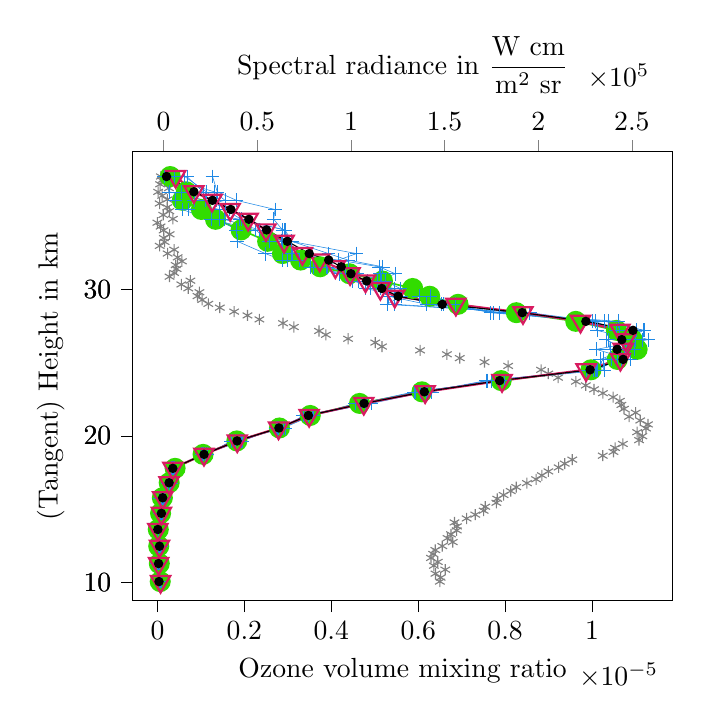
\begin{tikzpicture}

\definecolor{crimson2162796}{RGB}{216,27,96}
\definecolor{darkgray176}{RGB}{176,176,176}
\definecolor{dodgerblue30136229}{RGB}{30,136,229}
\definecolor{gray}{RGB}{128,128,128}
\definecolor{limegreen502200}{RGB}{50,220,0}

\begin{axis}[
axis x line=top,
tick align=outside,
x grid style={darkgray176},
xlabel={Spectral radiance in \(\displaystyle \frac{\text{W } \text{cm}}{\text{m}^2 \text{ sr}} \)},
xmin=-16446.367832345, xmax=271691.173814072,
xtick pos=right,
xtick style={color=gray},
y grid style={darkgray176},
ylabel={(Tangent) Height in km},
ymin=8.805976450571, ymax=39.3649129940911,
ytick pos=left,
ytick style={color=black}
]
\addplot [draw=gray, fill=gray, mark=asterisk, only marks]
table{%
x  y
147459.763013584 10.08
147907.155371426 10.35
145150.472966494 10.62
150380.513121916 10.89
144264.116900241 11.16
146373.292209872 11.42
142759.056905482 11.69
143924.248636755 11.96
145047.868936412 12.23
148783.225645754 12.5
154358.283940939 12.77
151584.575804699 13.04
153428.523695064 13.3
156472.805982049 13.57
156612.100322136 13.84
155306.603498135 14.11
161771.581300686 14.38
166399.162069621 14.64
170874.432498921 14.91
171739.961131439 15.18
177636.901344702 15.45
178133.041121706 15.72
181507.831873342 15.98
185325.192985734 16.25
188256.42072059 16.52
193973.50464238 16.79
198874.585791138 17.05
201939.411262633 17.32
205427.987113147 17.59
210892.618720805 17.86
214152.244283619 18.12
218189.022837926 18.39
234458.85383829 18.66
240188.653514636 18.92
241047.303353934 19.19
245191.926436868 19.46
253834.706091017 19.72
255579.706760119 19.99
252800.556317656 20.26
257529.47089241 20.52
258594.012830144 20.79
254461.087621174 21.06
248524.828859787 21.32
252050.252353648 21.59
245779.698649731 21.85
244413.373575122 22.12
243577.289908171 22.39
239978.430850513 22.65
234552.062163545 22.92
229800.021074123 23.18
225410.072935489 23.45
220128.190299816 23.71
210604.045551051 23.98
205385.515390711 24.25
201527.131686766 24.51
183953.255478903 24.78
171330.356179084 25.04
158109.195204561 25.31
151242.390537582 25.57
136913.986346471 25.84
116583.130655179 26.1
112989.071776433 26.37
98481.1102385779 26.63
86614.5913361595 26.9
82979.0013853583 27.16
69508.3030939949 27.43
63729.4827179448 27.69
51127.4263652965 27.95
44752.074027331 28.22
37647.7240377936 28.48
29988.5440034446 28.75
23857.9943363029 29.01
20578.4780994436 29.28
18097.0153984491 29.54
19114.9707534285 29.8
13128.1423625945 30.07
9435.06427123817 30.33
14304.5700774208 30.59
3152.1748416242 30.86
5594.09113682238 31.12
6919.31453123812 31.39
6442.14485626868 31.65
9757.54457487361 31.91
7494.27913525319 32.18
2118.90547958912 32.44
5605.17240973794 32.7
-2104.96221183688 32.96
535.4633119647 33.23
99.6475207179349 33.49
3218.42510479527 33.75
-18.7982665053022 34.02
-1625.29202175238 34.28
-3349.20684841696 34.54
4955.77733538067 34.8
-180.925078106093 35.07
3030.54909945026 35.33
1941.18312161005 35.59
-2138.07287607451 35.85
1972.08932925181 36.12
-793.699739957314 36.38
-2948.22552331652 36.64
2818.88514043493 36.9
-1901.49108306989 37.16
-982.218800611879 37.43
-1461.50561629362 37.69
};
\end{axis}

\begin{axis}[
tick align=outside,
tick pos=left,
x grid style={darkgray176},
xlabel={Ozone volume mixing ratio },
xmin=-5.66065374213903e-07, xmax=1.18500836147585e-05,
xtick style={color=black},
y grid style={darkgray176},
ymin=8.805976450571, ymax=39.3649129940911,
ytick style={color=black}
]
\addplot [semithick, limegreen502200, mark=*, mark size=3.5, mark options={solid}]
table {%
6.44060449417339e-08 10.0788394182732
4.28521182982422e-08 11.3060658223733
2.97768742996141e-08 12.489291714576
1.93396658687561e-08 13.6300950497901
7.2228473868563e-08 14.7299962717293
1.13421471326092e-07 15.7904620505408
2.70535423396723e-07 16.8129063358833
4.06417598242115e-07 17.798692829024
1.04986565929721e-06 18.749134931386
1.82685164418217e-06 19.6655000947865
2.80732456303667e-06 20.5490109224504
3.51548396793078e-06 21.4008442773599
4.65030734631e-06 22.2221364325659
6.08544360147789e-06 23.0139822120901
7.90916965343058e-06 23.7774376480819
9.97447386907879e-06 24.5135206594947
1.05811777757481e-05 25.2232124384117
1.10370310721919e-05 25.9074590546732
1.09241791506065e-05 26.5671731369065
1.05611534308991e-05 27.2032340298552
9.6248732006643e-06 27.8164899237427
8.25757433631225e-06 28.4077583763506
6.91641116645769e-06 28.9778277096296
6.26442488282919e-06 29.5274579658981
5.87282193009742e-06 30.0573821056521
5.17739499628078e-06 30.5683066270496
4.41800511907786e-06 31.0609126063955
3.74369005839981e-06 31.5358568908148
3.29360887008079e-06 31.9937727455081
2.87724174086179e-06 32.4352708003418
2.5351732801937e-06 33.2713464756911
1.92439779311826e-06 34.0485442112757
1.33678349811817e-06 34.7710105211694
1.01092177828832e-06 35.4425995548583
5.72321937397646e-07 36.0668941104285
6.64192668864416e-07 36.6472247971388
2.94370721576343e-07 37.6881607335064
};
\addplot [very thin, dodgerblue30136229, mark=+, mark size=2.5, mark options={solid}]
table {%
8.31315991929125e-08 10.0788394182732
2.57289193595127e-08 11.3060658223733
3.86755214742912e-08 12.489291714576
2.03031102146811e-08 13.6300950497901
7.33754740441154e-08 14.7299962717293
1.17819193505467e-07 15.7904620505408
2.37533780663007e-07 16.8129063358833
3.93242939659435e-07 17.798692829024
1.04644782048019e-06 18.749134931386
1.93156376396585e-06 19.6655000947865
2.73168186453472e-06 20.5490109224504
3.57835106590549e-06 21.4008442773599
4.55167825569777e-06 22.2221364325659
6.31087061115199e-06 23.0139822120901
7.59026405135516e-06 23.7774376480819
1.00232469611316e-05 24.5135206594947
1.06819440519013e-05 25.2232124384117
1.07516385469182e-05 25.9074590546732
1.03273781416586e-05 26.5671731369065
1.11911182410494e-05 27.2032340298552
1.02856448484585e-05 27.8164899237427
7.86321690986574e-06 28.4077583763506
6.52445757389578e-06 28.9778277096296
6.02076211012959e-06 29.5274579658981
4.90763555588964e-06 30.0573821056521
4.82893819979519e-06 30.5683066270496
4.187104141607e-06 31.0609126063955
3.59219552316981e-06 31.5358568908148
2.87848877421953e-06 31.9937727455081
2.48379082186046e-06 32.4352708003418
1.83832329252052e-06 33.2713464756911
1.81152728982766e-06 34.0485442112757
1.42552808888684e-06 34.7710105211694
1.64993729647838e-06 35.4425995548583
1.10794587466509e-06 36.0668941104285
2.68656476086708e-07 36.6472247971388
1.50752023309956e-07 37.6881607335064
};
\addplot [very thin, dodgerblue30136229, mark=+, mark size=2.5, mark options={solid}]
table {%
7.26255953640811e-08 10.0788394182732
3.67438551092404e-08 11.3060658223733
4.59048358849256e-08 12.489291714576
1.87965718600131e-08 13.6300950497901
6.31761520957497e-08 14.7299962717293
1.29955284442978e-07 15.7904620505408
2.74885067077808e-07 16.8129063358833
3.24936480833781e-07 17.798692829024
1.15042757667517e-06 18.749134931386
1.69407162517091e-06 19.6655000947865
2.89577793487287e-06 20.5490109224504
3.5595513259603e-06 21.4008442773599
4.83469546542447e-06 22.2221364325659
5.93797950719811e-06 23.0139822120901
7.86692596320911e-06 23.7774376480819
1.02778410709347e-05 24.5135206594947
1.01864678265168e-05 25.2232124384117
1.07890986479935e-05 25.9074590546732
1.09904206316465e-05 26.5671731369065
1.01118941578666e-05 27.2032340298552
1.00135104173955e-05 27.8164899237427
8.37894542517602e-06 28.4077583763506
5.27849663105183e-06 28.9778277096296
5.60813755305171e-06 29.5274579658981
4.78601547972648e-06 30.0573821056521
5.14603079382745e-06 30.5683066270496
5.1203831329439e-06 31.0609126063955
5.18115913659763e-06 31.5358568908148
4.38409931967209e-06 31.9937727455081
3.9372180472013e-06 32.4352708003418
3.08655778101098e-06 33.2713464756911
2.93726809195099e-06 34.0485442112757
1.88794028426851e-06 34.7710105211694
6.99462311782743e-07 35.4425995548583
1.55458601545098e-06 36.0668941104285
1.30501680784532e-06 36.6472247971388
1.68737467684789e-07 37.6881607335064
};
\addplot [very thin, dodgerblue30136229, mark=+, mark size=2.5, mark options={solid}]
table {%
8.24344298550451e-08 10.0788394182732
-1.6949656242507e-09 11.3060658223733
8.27403129189541e-08 12.489291714576
9.07976687393299e-09 13.6300950497901
7.51632371543588e-08 14.7299962717293
8.50116426850304e-08 15.7904620505408
3.04349903721223e-07 16.8129063358833
3.43694437596924e-07 17.798692829024
1.10885950588159e-06 18.749134931386
1.78166825367117e-06 19.6655000947865
2.93044389785409e-06 20.5490109224504
3.34667745138582e-06 21.4008442773599
4.79297920615092e-06 22.2221364325659
6.0520104776942e-06 23.0139822120901
7.8789939973621e-06 23.7774376480819
1.00738430008743e-05 24.5135206594947
1.02562782814388e-05 25.2232124384117
1.09702172943533e-05 25.9074590546732
1.1152628483128e-05 26.5671731369065
1.05495895949416e-05 27.2032340298552
1.00751443524672e-05 27.8164899237427
8.56528859294773e-06 28.4077583763506
5.45882347252554e-06 28.9778277096296
5.60801933052884e-06 29.5274579658981
5.44149486344946e-06 30.0573821056521
4.61472034498589e-06 30.5683066270496
4.31126655918691e-06 31.0609126063955
3.52397467378549e-06 31.5358568908148
2.97817182194658e-06 31.9937727455081
3.07333898692505e-06 32.4352708003418
2.57437842127868e-06 33.2713464756911
2.25999827345202e-06 34.0485442112757
1.23738321223107e-06 34.7710105211694
5.62196492887214e-07 35.4425995548583
8.40154239286019e-07 36.0668941104285
1.05171794259642e-06 36.6472247971388
6.77349259417689e-07 37.6881607335064
};
\addplot [very thin, dodgerblue30136229, mark=+, mark size=2.5, mark options={solid}]
table {%
5.14303647016325e-08 10.0788394182732
3.85226854190388e-08 11.3060658223733
4.39116566818719e-08 12.489291714576
1.73663410570367e-08 13.6300950497901
1.11181752625721e-07 14.7299962717293
1.00744300829701e-07 15.7904620505408
2.70011795416218e-07 16.8129063358833
3.63790908658898e-07 17.798692829024
1.0423928896404e-06 18.749134931386
1.91117661428426e-06 19.6655000947865
2.77850473557217e-06 20.5490109224504
3.47200998396579e-06 21.4008442773599
4.67859418121698e-06 22.2221364325659
5.90131697590045e-06 23.0139822120901
7.97624037938285e-06 23.7774376480819
9.86562101196232e-06 24.5135206594947
1.0876338325171e-05 25.2232124384117
1.00957774612322e-05 25.9074590546732
1.12857132061688e-05 26.5671731369065
1.06343060982518e-05 27.2032340298552
9.99966025461688e-06 27.8164899237427
7.66522042147357e-06 28.4077583763506
6.85780668898428e-06 28.9778277096296
6.26603859407147e-06 29.5274579658981
5.23418210449648e-06 30.0573821056521
5.05508233458319e-06 30.5683066270496
5.47485111236038e-06 31.0609126063955
5.09601739278699e-06 31.5358568908148
4.16143310973323e-06 31.9937727455081
3.08935414111936e-06 32.4352708003418
2.86301679130602e-06 33.2713464756911
2.34987458051111e-06 34.0485442112757
1.54016046078788e-06 34.7710105211694
1.43003139526621e-06 35.4425995548583
4.10824117618758e-07 36.0668941104285
5.47254202231354e-07 36.6472247971388
3.9190617116284e-07 37.6881607335064
};
\addplot [very thin, dodgerblue30136229, mark=+, mark size=2.5, mark options={solid}]
table {%
7.47236599671279e-08 10.0788394182732
2.92505309963516e-08 11.3060658223733
6.37675664409931e-08 12.489291714576
1.06350730563947e-08 13.6300950497901
9.97916161590012e-08 14.7299962717293
5.25386266858569e-08 15.7904620505408
3.12996652028975e-07 16.8129063358833
3.32207290406339e-07 17.798692829024
1.06341461965701e-06 18.749134931386
1.9472067627669e-06 19.6655000947865
2.76852918209682e-06 20.5490109224504
3.41052384430112e-06 21.4008442773599
4.70118233106877e-06 22.2221364325659
6.20374341954552e-06 23.0139822120901
7.68874747680833e-06 23.7774376480819
1.01067554054756e-05 24.5135206594947
1.04459971852224e-05 25.2232124384117
1.07790868199629e-05 25.9074590546732
1.07399150268897e-05 26.5671731369065
1.11864516333e-05 27.2032340298552
1.03752053473273e-05 27.8164899237427
7.71640022748418e-06 28.4077583763506
6.57543498098513e-06 28.9778277096296
5.44913878642497e-06 29.5274579658981
5.58700902190055e-06 30.0573821056521
5.24438316296412e-06 30.5683066270496
4.5893051643672e-06 31.0609126063955
3.89626698563251e-06 31.5358568908148
3.26550830046374e-06 31.9937727455081
3.10427154564154e-06 32.4352708003418
2.84530155972054e-06 33.2713464756911
2.87838923877995e-06 34.0485442112757
2.67620148467586e-06 34.7710105211694
2.70474232437366e-06 35.4425995548583
1.81602376073323e-06 36.0668941104285
1.37721014608882e-06 36.6472247971388
1.26672402486677e-06 37.6881607335064
};
\addplot [very thin, dodgerblue30136229, mark=+, mark size=2.5, mark options={solid}]
table {%
7.93011983413589e-08 10.0788394182732
3.47732575889031e-08 11.3060658223733
2.2730289689616e-08 12.489291714576
1.65878595290739e-08 13.6300950497901
9.67981656793524e-08 14.7299962717293
1.52098680646162e-07 15.7904620505408
2.68792917912042e-07 16.8129063358833
3.43860903788559e-07 17.798692829024
1.01522200408184e-06 18.749134931386
1.79714926196721e-06 19.6655000947865
2.78792260974811e-06 20.5490109224504
3.46837918552798e-06 21.4008442773599
4.9234718862905e-06 22.2221364325659
6.18837967712159e-06 23.0139822120901
7.5676845619093e-06 23.7774376480819
1.01246086945866e-05 24.5135206594947
1.0588150827914e-05 25.2232124384117
1.04090286457663e-05 25.9074590546732
1.03794487651362e-05 26.5671731369065
1.10188583202159e-05 27.2032340298552
1.05914251924593e-05 27.8164899237427
7.87153104969555e-06 28.4077583763506
6.19330754373104e-06 28.9778277096296
5.32090963549178e-06 29.5274579658981
5.13830111332401e-06 30.0573821056521
4.48873141687058e-06 30.5683066270496
4.49368187394245e-06 31.0609126063955
3.87524589013597e-06 31.5358568908148
4.16605636573467e-06 31.9937727455081
4.58099931814446e-06 32.4352708003418
3.0689385185407e-06 33.2713464756911
2.90924106790376e-06 34.0485442112757
1.92413729402633e-06 34.7710105211694
1.56971589684117e-06 35.4425995548583
1.36079643076942e-06 36.0668941104285
1.12582911760758e-06 36.6472247971388
6.28272375686684e-07 37.6881607335064
};
\addplot [thick, crimson2162796, mark=triangle, mark size=4, mark options={solid,rotate=180,fill opacity=0}]
table {%
7.25974156282327e-08 10.0788394182732
2.67762551315503e-08 11.3060658223733
4.74487459017362e-08 12.489291714576
9.67618050692368e-09 13.6300950497901
9.12342808733294e-08 14.7299962717293
1.20776529113943e-07 15.7904620505408
2.67257324916527e-07 16.8129063358833
3.55847674308641e-07 17.798692829024
1.07050034773987e-06 18.749134931386
1.83643550434788e-06 19.6655000947865
2.78589614870084e-06 20.5490109224504
3.49026603803714e-06 21.4008442773599
4.74759346081428e-06 22.2221364325659
6.15935235367565e-06 23.0139822120901
7.92863013138352e-06 23.7774376480819
9.8621017066277e-06 24.5135206594947
1.06514170289884e-05 25.2232124384117
1.07150419380077e-05 25.9074590546732
1.07756436215131e-05 26.5671731369065
1.06420143839491e-05 27.2032340298552
9.73434372836227e-06 27.8164899237427
8.41064623578529e-06 28.4077583763506
6.86653153012694e-06 28.9778277096296
5.46025991165052e-06 29.5274579658981
5.12864455550519e-06 30.0573821056521
4.78774351574862e-06 30.5683066270496
4.43214601791373e-06 31.0609126063955
4.09291423220886e-06 31.5358568908148
3.73288067579724e-06 31.9937727455081
3.33501958927689e-06 32.4352708003418
2.91595754308495e-06 33.2713464756911
2.49657664552088e-06 34.0485442112757
2.08733009007059e-06 34.7710105211694
1.67355193607363e-06 35.4425995548583
1.25678772906307e-06 36.0668941104285
8.37927987365519e-07 36.6472247971388
4.19350544889384e-07 37.6881607335064
};
\addplot [black, mark=*, mark size=1.5, mark options={solid}]
table {%
3.62956843989365e-08 10.0788394182732
2.67011816708239e-08 11.3060658223733
4.74544145085064e-08 12.489291714576
9.48144929276078e-09 13.6300950497901
9.13362086451027e-08 14.7299962717293
1.20328824570024e-07 15.7904620505408
2.68087041201918e-07 16.8129063358833
3.53207128810194e-07 17.798692829024
1.0719023614733e-06 18.749134931386
1.83262919261261e-06 19.6655000947865
2.79527409403845e-06 20.5490109224504
3.47353434464988e-06 21.4008442773599
4.75391272261123e-06 22.2221364325659
6.1399075162147e-06 23.0139822120901
7.8749713185963e-06 23.7774376480819
9.95398861108484e-06 24.5135206594947
1.0713124741107e-05 25.2232124384117
1.05757669679967e-05 25.9074590546732
1.06831495285149e-05 26.5671731369065
1.09410886905668e-05 27.2032340298552
9.8576105420837e-06 27.8164899237427
8.39295729959107e-06 28.4077583763506
6.55244557187671e-06 28.9778277096296
5.53870752911986e-06 29.5274579658981
5.16147010453556e-06 30.0573821056521
4.81338536883742e-06 30.5683066270496
4.45214596461242e-06 31.0609126063955
4.22714898085563e-06 31.5358568908148
3.94093843574795e-06 31.9937727455081
3.49262926715456e-06 32.4352708003418
2.98819174257628e-06 33.2713464756911
2.51015606394261e-06 34.0485442112757
2.10573988006852e-06 34.7710105211694
1.68876906821657e-06 35.4425995548583
1.26482532209324e-06 36.0668941104285
8.3801883098714e-07 36.6472247971388
2.08833305398235e-07 37.6881607335064
};
\end{axis}

\end{tikzpicture}
}
	%\includegraphics[width =0.99 \columnwidth]{FirstRecRes.png}
	\caption{Plot of the true ozone profile (\mycircle{circ}), posterior samples (\myplus{plus}), and posterior mean (\myseccircle{seccirc}). We display the optimal regularised solution (\mytriangle{tri}) and the simulated data (\mysecstar{gray}) in spectral radiance.}
	\label{fig:Results}
\end{figure}



\section{four hyperameters, t-walk, TT approx, and RTO}

\begin{itemize}
	\item t-walk ref
	\item motivation why more hyper-parameters, explain parabula
	\item how sample from them, compared to TT approx
	\item explain Rosenblatt and SIRT trasnport
	\item RTO
\end{itemize}


\begin{figure}[thb!]
	\centering
	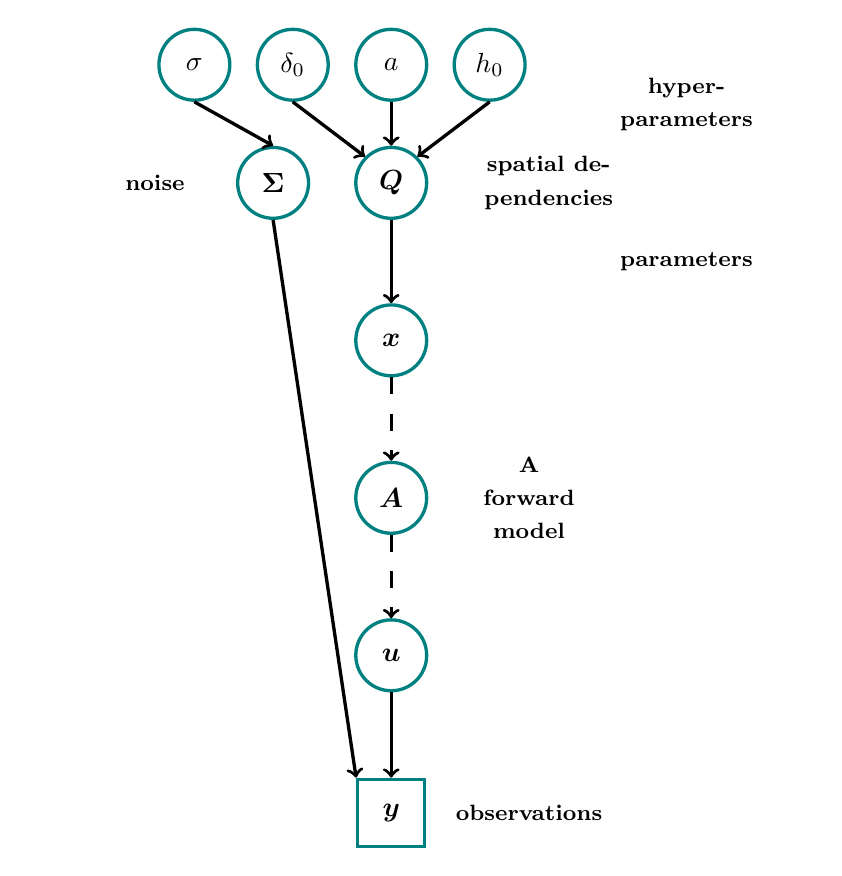
\begin{tikzpicture}
		\node[roundnode2] at (0,6) (Q)     {$\bm{Q}$};
		\node[roundnode2] at (0,4) (x)     {$\bm{x}$};
		\node[roundnode2] at (0,2) (A)    {$\bm{A}$};
		\node[roundnode2] at (0,0) (u)    {$\bm{u}$};
		\node[rectnode] at (0,-2) (y)    {$\bm{y}$};
		\node[roundnode2] at (-1.5,6) (S)    {$\bm{\Sigma}$};
		\node[roundnode2] at (-2.5,7.5) (s)    {$\sigma$};
		\node[roundnode2] at (-1.25,7.5) (d)    {$\delta_0$};
		\node[roundnode2] at (0,7.5) (a)    {$a$};
		\node[roundnode2] at (1.25,7.5) (h0)    {$h_0$};
		
		%text
		%\draw (-1,2.5) node[align=center, text width=1.5cm] {\footnotesize \textbf{hydrostatic \\ equation}};
		\draw (1.75,2) node[align=center, text width=1.5cm] {\footnotesize \textbf{A \\ forward model }};
		%\draw (6.75,-1.5) node[align=center, text width=2.5cm] {\footnotesize \textbf{hyper\-parameters}};
		%\draw (5.5,-1.5) node[align=center, text width=0.5cm] { $\bm{\theta}$};
		\draw (1.75,-2) node[align=center, text width=3cm] {\footnotesize \textbf{observations}};
		\draw (3.75,7) node[align=center, text width=3cm] {\footnotesize \textbf{hyper-\\parameters}};
		\draw (3.75,5) node[align=center, text width=3cm] {\footnotesize \textbf{parameters}};
		\draw (2,6) node[align=center, text width=3cm] {\footnotesize \textbf{spatial dependencies}};
		%\draw (-1.4,-2.3) node[align=center, text width=3cm] {\footnotesize \textbf{hyper-prior}};
		\draw (-3,6) node[align=center, text width=3cm] {\footnotesize \textbf{noise}};
		% Calligraphic brace
		%\draw[very thick, decorate,decoration = {brace}] (5,-1) --  (5,-2);
		
		%Lines
		\draw[->, very thick] (S.south) -- (y.north west);
		\draw[->, very thick] (s.south) -- (S.north);
		\draw[->, very thick] (u.south) -- (y.north);
		\draw[->, mydotted, very thick] (A.south) -- (u.north);
		\draw[->, mydotted,  very thick] (x.south) -- (A.north);
		\draw[->, very thick] (a.south) -- (Q.north); 
		\draw[->, very thick] (h0.south) -- (Q.north east); 
		\draw[->, very thick] (d.south) -- (Q.north west); 
		\draw[->, very thick] (Q.south) -- (x.north); 
		
		
	\end{tikzpicture} 
	\caption[short text]{text}
\end{figure}

\begin{itemize}
	\item  define priors
	\item how solve inverse and determinant
	\item how many steps, integrated autocorrealtion time
	\item relative error
\end{itemize}

\begin{figure}[h]
	\centering
	%\includegraphics[width=\textwidth]{DeltaSamp.png}
	\scalebox{0.66}{\input{allHistoRes.pdf_tex}}
	\caption[]{text}
	\label{fig:Results}
\end{figure}


\begin{figure}[h]
	\centering
	%\includegraphics[width=\textwidth]{DeltaSamp.png}
	\scalebox{0.66}{\input{DeltaSamp.pdf_tex}}
	\caption[]{text}
	\label{fig:Results}
\end{figure}


\begin{figure}[h]
	\centering
	%\includegraphics[width=\textwidth]{DeltaSamp.png}
	\scalebox{0.66}{\input{O3Results.pdf_tex}}
	\caption[]{text}
	\label{fig:Results}
\end{figure}



\subsection{Sampling}

\subsection{ Rosenblatt Transform}
\subsection{(Squared) Inverse Rosenblatt Transform}
\subsection{Tensor-Train Approximation}

\begin{figure}[h]
	\centering
	%\includegraphics[width=\textwidth]{DeltaSamp.png}
	\scalebox{0.66}{\input{HistSamp.pdf_tex}}
	\caption[]{TTSIRT output}
	\label{fig:Results}
\end{figure}
\begin{figure}[h]
	\centering
	%\includegraphics[width=\textwidth]{DeltaSamp.png}
	\scalebox{0.66}{\input{DeltaSIRTSamp.pdf_tex}}
	\caption[]{text}
	\label{fig:Results}
\end{figure}

\begin{figure}[h]
	\centering
	%\includegraphics[width=\textwidth]{DeltaSamp.png}
	\scalebox{0.66}{\input{SIRTO3Results.pdf_tex}}
	\caption[]{text}
	\label{fig:Results}
\end{figure}


\section{Temperature and pressure hyperameters, tt-approx}

\begin{table}
	\centering
	\begin{tabular}{ |c||c|c|c|c|   }
		\hline
		model context& burn in& steps & dimension & time\\ 
		\hhline{|=||=|=|=|=|}
		$\bm{x}$, MTC& 4 & \makecell[b]{ $10^{-10}$} &2 &\\ \hline
		$\bm{x}$, t-walk& 500& &4 &\\ \hline
		$\bm{p}$, t-walk & 500& &5 &\\ \hline
		$\bm{t}$, t-walk & 2500 & &13 &\\
		\hline
	\end{tabular}
	\caption{T walk settting}
	\label{tab:}
\end{table}

\begin{table}
	\centering
	\begin{tabular}{ |c||c|c|c|c|c|  }
		\hline
		model context& \makecell{max number \\of swaps (TT-cross)}& \makecell{maximum relative \\ error (TT-cross)}&\makecell{QMC samples \\per dimension}& \makecell{SIRT\\ error} & time\\ \hline
		\hline
		$\bm{x}$ & 4 & $10^{-10}$ &4& &\\ \hline
		$\bm{p}$ & 5& &5& &\\ \hline
		$\bm{t}$ & 5 & &13& &\\ 
		\hline
	\end{tabular}
	\caption{Sirt and TT settting}
	\label{tab:}
\end{table}

\begin{itemize}
	\item updating scheme
\end{itemize}

\begin{figure}[thb!]
	\centering
	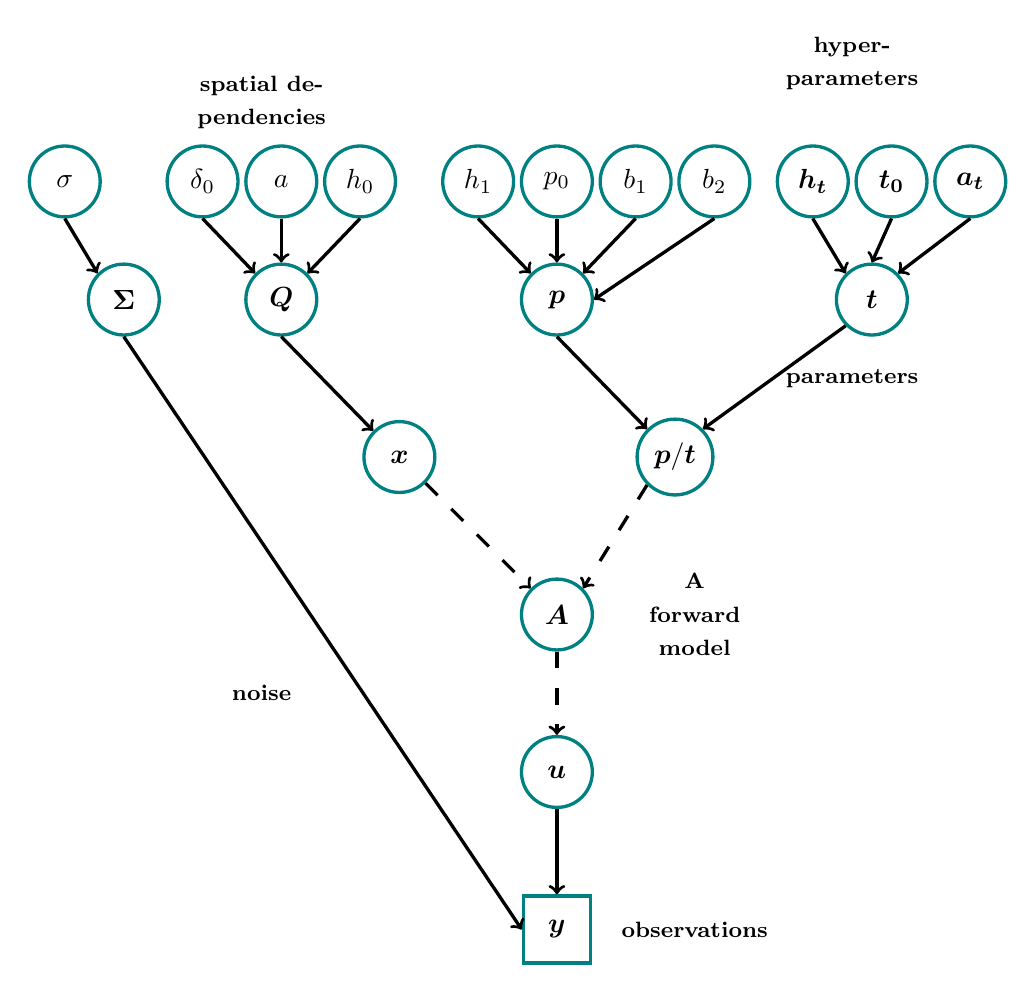
\begin{tikzpicture}
		\node[roundnode2] at (-3.5,6) (Q)     {$\bm{Q}$};
		\node[roundnode2] at (-2,4) (x)     {$\bm{x}$};
		\node[roundnode2] at (0,2) (A)    {$\bm{A}$};
		\node[roundnode2] at (0,0) (u)    {$\bm{u}$};
		\node[rectnode] at (0,-2) (y)    {$\bm{y}$};
		\node[roundnode2] at (-5.5,6) (S)    {$\bm{\Sigma}$};
		\node[roundnode2] at (-6.25,7.5) (s)    {$\sigma$};
		\node[roundnode2] at (-4.5,7.5) (d)    {$\delta_0$};
		\node[roundnode2] at (-3.5,7.5) (a)    {$a$};
		\node[roundnode2] at (-2.5,7.5) (h0)    {$h_0$};
		\node[roundnode2] at (4,6) (t)     {$\bm{t}$};
		\node[roundnode2] at (0,6) (p)     {$\bm{p}$};
		\node[roundnode2] at (1.5,4) (pt)     {$\bm{p}/\bm{t}$};
		\node[roundnode2] at (1,7.5) (b1)    {$b_1$};
		\node[roundnode2] at (2,7.5) (b2)    {$b_2$};
		\node[roundnode2] at (-1,7.5) (h1)    {$h_1$};
		\node[roundnode2] at (-0,7.5) (p0)    {$p_0$};
		\node[roundnode2] at (3.25,7.5) (ht)    {$\bm{h_t}$};
		\node[roundnode2] at (4.25,7.5) (t0)    {$\bm{t_0}$};
		\node[roundnode2] at (5.25,7.5) (at)    {$\bm{a_t}$};
		
		\draw (1.75,2) node[align=center, text width=1.5cm] {\footnotesize \textbf{A \\ forward model }};
		
		\draw (1.75,-2) node[align=center, text width=3cm] {\footnotesize \textbf{observations}};
		\draw (3.75,9) node[align=center, text width=3cm] {\footnotesize \textbf{hyper-\\parameters}};
		\draw (3.75,5) node[align=center, text width=3cm] {\footnotesize \textbf{parameters}};
		\draw (-3.75,8.5) node[align=center, text width=3cm] {\footnotesize \textbf{spatial dependencies}};
		\draw (-3.75,1) node[align=center, text width=3cm] {\footnotesize \textbf{noise}};
		
		
		%Lines
		\draw[->, very thick] (S.south) -- (y.west);
		\draw[->, very thick] (s.south) -- (S.north west);
		\draw[->, very thick] (u.south) -- (y.north);
		\draw[->, mydotted, very thick] (A.south) -- (u.north);
		\draw[->, mydotted,  very thick] (x.south east) -- (A.north west);
		\draw[->, very thick] (p.south) -- (pt.north west);
		\draw[->, very thick] (t.south west) -- (pt.north east);
		\draw[->,  mydotted, very thick] (pt.south west) -- (A.north east);
		\draw[->, very thick] (h1.south) -- (p.north west);
		\draw[->, very thick] (p0.south) -- (p.north);
		\draw[->, very thick] (b1.south) -- (p.north east); 
		\draw[->, very thick] (b2.south) -- (p.east); 
		
		\draw[->, very thick] (a.south) -- (Q.north); 
		\draw[->, very thick] (h0.south) -- (Q.north east); 
		\draw[->, very thick] (d.south) -- (Q.north west); 
		\draw[->, very thick] (Q.south) -- (x.north west); 
		\draw[->, very thick] (ht.south) -- (t.north west);
		\draw[->, very thick] (t0.south) -- (t.north);
		\draw[->, very thick] (at.south) -- (t.north east);
		
	\end{tikzpicture} 
	\caption[short text]{text}
\end{figure}

\begin{table}
	\centering
\begin{tabular}{ |c||c|c|c|c|   }
	\hline
	& &\multicolumn{2}{|c|}{TT bounds}&\\
	\hline
	model parameters& priors&\makecell{lower}& \makecell{upper\\
	}&Context\\
	\hline

	$\gamma$ & $\mathcal{T}(1,10^{-10})$ &- &-& $\bm{x}$\\ \hhline{|=||=|=|=|=|}
	$\delta$ &$\mathcal{T}(1,10^{-10})$ & -&-& $\bm{x}$\\ \hline
	%$\gamma$ & $\mathcal{N}(2.58e-9,2.58e-11)$ &2.45e-9&2.7e-9 &$\bm{x}$\\
	%$\delta_0$ &  $\mathcal{N}(0.8e-4,0.75e-5)$& 4e-5 & 1.1e-4&$\bm{x}$\\
	$a_0$ &  $\mathcal{T}(3,1e6)$& 1e-15&1e-5&$\bm{x}$\\ \hline
	$h_0$ &  $\mathcal{N}(31.35,1)$&27 &35&$\bm{x}$\\ \hline
	$h_{p,1}$ &  $\mathcal{N}(34.3,0.5)$& 32.8&35.64&$\bm{p/t}$\\ \hline
	$p_0$ &  $\mathcal{N}(6.5,0.1)$&6.17 &6.73&$\bm{p/t}$\\ \hline
	$b_1$ &  $\mathcal{N}(0.15,0.0051)$& 0.138  &0.167&$\bm{p/t}$\\ \hline
	$b_2$ & $\mathcal{N}(0.13,0.067)$& 0&0.32&$\bm{p/t}$\\ \hline
	$h_{t,0}$ &  $\mathcal{N}(11,0.5)$&9.6 &12.4&$\bm{p/t}$\\ \hline
	$h_{t,1}$ &  $\mathcal{N}(20,3)$&11.6 &28.4&$\bm{p/t}$\\ \hline
	$h_{t,2}$ &  $\mathcal{N}(32,1)$&29.2 &34.8&$\bm{p/t}$\\ \hline
	$h_{t,3}$ &  $\mathcal{N}(47,2)$&41.4 &52.6&$\bm{p/t}$\\ \hline
	$h_{t,4}$ &  $\mathcal{N}(51,2)$&45.4 &56.6&$\bm{p/t}$\\ \hline
	$h_{t,5}$ &  $\mathcal{N}(71,2)$&65.4 &76.6&$\bm{p/t}$\\ \hline
	$a_{t,1}$ &  $\mathcal{N}(-6.5,0.01)$&-6.528 &-6.472&$\bm{p/t}$\\ \hline
	$a_{t,2}$ &  $\mathcal{N}(1,0.01)$&0.972 &1.028&$\bm{p/t}$\\ \hline
	$a_{t,3}$ &  $\mathcal{N}(2.8,0.1)$&2.52 &3.078&$\bm{p/t}$\\ \hline
	$a_{t,4}$ &  $\mathcal{N}(-2.8,0.01)$&-2.828 &-2.772&$\bm{p/t}$\\ \hline
	$a_{t,5}$ & $\mathcal{N}(-2,0.01)$ &-2.028 &-1.972&$\bm{p/t}$\\ \hline
	$t_{0}$ &  $\mathcal{N}(288,2)$& 282.54 &293.75&$\bm{p/t}$\\
	\hline
\end{tabular}
\caption{Gaussian $\mathcal{N}(\mu,\sigma)$ and gamma distribution $\mathcal{T}(\alpha = \text{scale}, \beta = \text{rate})$
	Bounds for t and p 2.8 times the variance around the mean
round pressure approx and  test if would work with previous gamma prior or fix gamma prior with set values}
\label{tab:1}
\end{table}

\begin{figure}[t!]
	\centering
	\begin{subfigure}[]{.49\columnwidth}
		\centering
		\scalebox{0.25}{\input{tempHistRes0.pdf_tex}}
		%\caption{}
	\end{subfigure}%
	\begin{subfigure}[]{.49\columnwidth}
	\centering
	\scalebox{0.25}{\input{tempHistRes1.pdf_tex}}
	%\caption{}
\end{subfigure}
	\begin{subfigure}[]{.49\columnwidth}
		\centering
		\scalebox{0.25}{\input{tempHistRes2.pdf_tex}}
		%\caption{}
	\end{subfigure}
	\begin{subfigure}[]{.49\columnwidth}
	\centering
	\scalebox{0.25}{\input{tempHistRes3.pdf_tex}}
	%\caption{}
\end{subfigure}
	\begin{subfigure}[]{.49\columnwidth}
	\centering
	\scalebox{0.25}{\input{tempHistRes4.pdf_tex}}
	%\caption{}
\end{subfigure}
	\caption{show that t- walk works for posterior}
\end{figure}


\begin{figure}[t!]
	\centering
	\begin{subfigure}[]{.49\columnwidth}
		\centering
		\scalebox{0.25}{\input{TempPostHistSamp0.pdf_tex}}
		%\caption{}
	\end{subfigure}%
	\begin{subfigure}[]{.49\columnwidth}
		\centering
		\scalebox{0.25}{\input{TempPostHistSamp1.pdf_tex}}
		%\caption{}
	\end{subfigure}
	\begin{subfigure}[]{.49\columnwidth}
		\centering
		\scalebox{0.25}{\input{TempPostHistSamp2.pdf_tex}}
		%\caption{}
	\end{subfigure}
	\begin{subfigure}[]{.49\columnwidth}
		\centering
		\scalebox{0.25}{\input{TempPostHistSamp3.pdf_tex}}
		%\caption{}
	\end{subfigure}
	\begin{subfigure}[]{.49\columnwidth}
		\centering
		\scalebox{0.25}{\input{TempPostHistSamp4.pdf_tex}}
		%\caption{}
	\end{subfigure}
	\caption{show that TT does not work for posterior}
\end{figure}
\begin{figure}[t!]
	\centering
	\begin{subfigure}[]{.49\columnwidth}
		\centering
		\scalebox{0.25}{\input{TempPriorHistSamp0.pdf_tex}}
		%\caption{}
	\end{subfigure}%
	\begin{subfigure}[]{.49\columnwidth}
		\centering
		\scalebox{0.25}{\input{TempPriorHistSamp1.pdf_tex}}
		%\caption{}
	\end{subfigure}
	\begin{subfigure}[]{.49\columnwidth}
		\centering
		\scalebox{0.25}{\input{TempPriorHistSamp2.pdf_tex}}
		%\caption{}
	\end{subfigure}
	\begin{subfigure}[]{.49\columnwidth}
		\centering
		\scalebox{0.25}{\input{TempPriorHistSamp3.pdf_tex}}
		%\caption{}
	\end{subfigure}
	\begin{subfigure}[]{.49\columnwidth}
		\centering
		\scalebox{0.25}{\input{TempPriorHistSamp4.pdf_tex}}
		%\caption{}
	\end{subfigure}
	\caption{show that TT works for prior}
\end{figure}


\begin{figure}[t!]
	\centering
	\begin{subfigure}[]{.49\columnwidth}
		\centering
		\scalebox{0.42}{\input{SIRTALLTempResults.pdf_tex}}
		\caption{}
	\end{subfigure}%
	\begin{subfigure}[]{.49\columnwidth}
		\centering
		\scalebox{0.42}{\input{SIRTALLPressResults.pdf_tex}}
		\caption{}
	\end{subfigure}
	\caption{}
\end{figure}

\begin{figure}[h]
	\centering
	\scalebox{0.66}{\input{SIRTALLO3Results.pdf_tex}}
	\caption[]{text}
	\label{fig:Results}
\end{figure}



\begin{figure}[h]
	\centering
	\scalebox{0.66}{\input{PTHistSampP.pdf_tex}}
	\caption[]{pritor}
	\label{fig:Results}
\end{figure}

\begin{figure}[h]
	\centering
	\scalebox{0.66}{\input{TTHistSampP.pdf_tex}}
	\caption[]{posteriore doesnt work with TT format}
	\label{fig:Results}
\end{figure}


\begin{figure}[h]
	\centering
	\scalebox{0.66}{\input{pressHistRes.pdf_tex}}
	\caption[]{t-walk does work with posterioer}
	\label{fig:Results}
\end{figure}

\begin{figure}[h]
	\centering
	\scalebox{0.66}{\input{IRTPHistRes.pdf_tex}}
	\caption[]{normal IRT does work with posterioer}
	\label{fig:Results}
\end{figure}


\begin{figure}[h]
	\centering
	\scalebox{1}{\input{PTHistSampT1.pdf_tex}}
	\caption[]{priors work}
	\label{fig:Results}
\end{figure}


\begin{figure}[h]
	\centering
	\scalebox{1}{\input{TempPriorHistSamp.pdf_tex}}
	\caption[]{priorsTT work}
	\label{fig:Results}
\end{figure}


\begin{figure}[h]
	\centering
	\scalebox{1}{\input{PTHistSampT2.pdf_tex}}
	\caption[]{priors work}
	\label{fig:Results}
\end{figure}



%\chapter{Application to Cube-Sat}
\label{ch:3-application}
In this chapter, we would like to introduce the Atmospheric model and how we apply this to our earlier presented sampling algorithms.
Firstly, we like to formulate the linear forward model and showcase with one specific measurement setup how we implemented the marginal and then conditional (MTC) sampler.
\mccorrect{Maybe another sampler.}
In doing so, we utilize a Metropolis within Gibbs sampler to sample hyper-parameters.
Afterward, we use the Randomize then Optimize (RTO) method to draw a sample from the conditional posterior density function.
This gives us a sample from the \mccorrect{full} posterior density.

\section{The forward model}
\label{subsec:atmosModel}
\begin{figure}[thb!]
\centering \input{figures/LIMB.pdf_tex}
\caption[The Forward model describing $n$ atmospheric layers and $m$ measurement processes.]{\textbf{The Forward model describing $n$ atmospheric layers and $m$ measurement processes.} The Cube-Sat is located at a height of $300$km, where each of the $m$ measurements is described through a tangent height $h_t$. Through the measurements we try to capture the Ozone profile, an example is displayed in light green, between $5$km and $90$km, below and above it we set the volume mixing ratio of Ozone to zero.
In order to do so we discretize the Ozone profile into $n$ atmospheric layers starting from the earth in black at ground level set to a height of $0$km.
This gives us a Markov random field with $x^{(1)}, \dots, x^{(n)}$ parameters
Along the golden line, we solve the path integral as formulated in Equation \ref{eq:pathInt} for each measurement.}
\label{fig:forModel}
\end{figure}
We introduce a linear forward model to describe the measurement process of a microwave sounder at the limb of the atmosphere, around $300$km above the ground of the earth.
Traces gases emit thermal radiation in the microwave regime, which we can capture with a resonator.
This resonator is a whispering gallery resonator, which can capture microwaves in the THz domain as well as light in the optical domain.
The microwaves are shifted towards the optical domain and we are able to read out a signal, without cooling down the measurement device.
Not needing the cooling unit allows us to fit everything we need to measure trace gases in the atmosphere into a Cube-Sat.
Depending on the angle we can measure different atmospheric layers and their traces gases, in this case, we focus on the volume mixing ratio (VMR) of Ozone $\bm{x} \in \mathbb{R}^n$.
The forward model $ \bm{F} \in \mathbb{R}^{m \times n}$  maps the Ozone profile to the space of all measurable, then can measure the data $\bm{y} \in \mathbb{R}^m$.
\begin{align}
   \bm{y} =  \bm{F}  \bm{x} + \gamma
\end{align} 

The forward model is defined through the number of atmospheric layers $n$ and measurements $m$, which are independent of each other as seen in Figure \ref{fig:forModel}.
Each measurement for a specific wavelength $\sigma$ can be described with a path integral (golden in Figure \ref{fig:forModel}) along $r$ the line of sight of the instrument, starting from $r_{obs}$, the location of the CubeSat through the atmosphere until $r_{\infty}$:
\begin{align}
\label{eq:pathInt}
     \int^{r_{\infty}}_{r_{obs}} S(\sigma) x(r) k_m(\sigma) \eta(r) \text{d}r \, ,
\end{align}
where $S(\sigma)$ is the Planck function, $\eta(r)$ number density of air, $k_m(\sigma) $ absorption cross section and $x(r)$ is the volume mixing ratio of ozone.
We assume thermal equilibrium when calculating the Planck function and discrete the atmosphere to calculate the integral.
Below a height of $5$km and above a height of $90$km, we set the volume mixing ratio of Ozone to zero.
Each measurement is defined according to a tangent height $h_t$.
The measurement is perturbed with white noise, which we describe through the hyper-parameter $\gamma$.
For further reading we refer to the Envisat MIPAS Handbook \cite{fischer2000envisat} and appendix \ref{ap:RTE}.

Based on the forward model, also displayed in figure \ref{fig:forModel}, we set up a linear-Gaussian hierarchical Bayesian model.
\begin{subequations}
    \begin{align}
        \bm{y}|\bm{x}, \gamma &\sim \mathcal{N}(\bm{F}\bm{x}, \gamma^{-1}\bm{I}) \\
        \bm{x}| \delta &\sim  \mathcal{N}( 0, (\delta \bm{L})^{-1}  ) \\
        \pi(\gamma) &\propto \gamma^{\alpha_\gamma -1} \exp{(- \beta_\gamma \gamma)} \label{eq:gamma} \\
        \pi(\delta) &\propto \delta^{\alpha_\delta -1} \exp{(- \beta_\delta \delta)} \label{eq:delta}
    \end{align}
\end{subequations}


The hyper-parameters $\gamma$ and $\delta$ are described with relatively uninformative priors.
The coefficients of the gamma distributions in Equations \ref{eq:gamma} - \ref{eq:delta} are $\alpha_\gamma = \alpha_\delta = 1 $ and $\beta_\gamma = \beta_\delta = 10^{-4}$, here we use the paper of Fox and Norton as a reference \cite{fox2016fast}.

We describe the spatial dependencies of the Ozone profile with the lumping constant $\delta$, which gives a measure of how strongly the individual parameters interact, and a graph Laplacian to describe maximum cliques and neighborhoods.
The parameters $x^{(1)}, \dots, x^{(n)}$ are normally distributed and form a Gaussian Markov random field (GMRF).
\begin{align}
    x^{(i)}| \partial x^{(i)} \sim  \mathcal{N}( |\partial^{(i)}|^{-1} \sum\nolimits_{j\in \partial x^{(i)} } x_j , (\delta |\partial^{(i)}|)^{-1}  )
\end{align}
Here $\partial x^{(i)}$ is the neighborhood of $x^{(i)}$ and $|\partial^{(i)}|$ the number of nodes connected to $x^{(i)}$ in that GMRF.
We relate the GMRF in our hierarchical Bayesian model with the precision matrix of the parameters $\bm{Q}= \delta \bm{L}$.
The Matrix L is constructed such that one parameter $x_i$ is only affected by its neighboring parameters $x_{i-1}$ and $x_{i+1}$.
We implement non-periodic boundaries.
\begin{align}
 \bm{Q}= \delta \bm{L} =
    \delta
\begin{bmatrix}
     1 & -1 & 0 & \cdots & 0\\
     -1 & 2 & -1 & \ddots & \vdots \\
     0 & \ddots & \ddots & \ddots & 0 \\ 
     \vdots & \ddots  & -1 & 2 & -1 \\
       0 & \cdots & 0 & -1 & 1 \\
\end{bmatrix}  
\end{align}

Given this setup, we can generate samples from the marginal posterior distribution $\lambda, \gamma | \bm{y}$ for the hyper-parameters $\gamma$ and $\lambda = \delta / \gamma$.
So that the marginal posterior is:
\begin{align}
    \pi(\lambda, \gamma | \bm{y})
    \propto ( \lambda \gamma)^{n/2} \exp{ \Bigg( - \frac{1}{2} g ( \lambda) - \frac{\gamma}{2} f ( \lambda) \Bigg) } \, .
    \label{eq:MargPostAppl}
\end{align}
We introduce the function $f(\lambda)$ and $g(\lambda)$ as:
\begin{subequations}
\label{eq:fandg}
\begin{align}
    f ( \lambda) &= \bm{y}^T \bm{y} - (\bm{F}^T \bm{y})^T (\bm{F}^T  \bm{F} + \lambda \bm{L})^{-1} (\bm{F}^T \bm{y})  \label{eq:f} \, \,  \text{and} \\
    g(\lambda) &= \log \det (\bm{F}^T  \bm{F} + \lambda \bm{L}) \label{eq:g}\,,
\end{align}
\end{subequations}
where $g(\lambda)$ accounts for the ratio of determinants, which is usually expensive to calculate.
We plotted those functions in Figure \ref{fig:fandg} for a large range of $\lambda$ and will use their behavior to our advantage later this in section.
%As displayed in Figure \ref{fig:fandg}, those functions behave quite well and we will use that to our advantage as we need to calculate the difference of those functions when sampling $\lambda$.

To generate a Markov chain of hyper-parameter samples we choose a so-called Metropolis-within-Gibbs algorithm, see Algorithm \ref{alg:MwG}.
We use a Metropolis-Hastings algorithm to draw $\lambda$ samples from $\pi(\lambda |  \bm{y}, \gamma )$ and then do a Gibbs step in $\gamma$ direction, where we draw a sample from the distribution \ref{eq:gammaPrior}.
\begin{subequations}
\begin{align}
    \label{eq:gammaPrior}
     \gamma |  \bm{y}, \lambda &\sim \Gamma \bigg( \frac{m}{2} + \alpha_\delta + \alpha_\gamma, \frac{1}{2} f (\lambda ) + \beta_\gamma + \beta_\delta \lambda \bigg)\\
     \label{eq:lamPrior}
     \pi(\lambda | \bm{y}, \gamma) &\propto \lambda^{n/2+\alpha_\delta -1} \exp{\bigg( - \frac{1}{2} g ( \lambda) - \frac{\gamma}{2} f ( \lambda) - \beta_\delta \gamma \lambda \bigg)}
\end{align} 
\end{subequations}
If we like to utilize a Metropolis-Hastings algorithm on the probability density Function \ref{eq:lamPrior} we need to evaluate the Ratio \ref{eq:lamRatio}, to do a step in $\lambda + \Delta \lambda $ direction and to generate a new candidate $\lambda'$.
\begin{align}
\label{eq:lamRatio}
    \frac{\pi(\lambda' |  \bm{y}, \gamma ) }{\pi(\lambda |  \bm{y}, \gamma) } \propto \bigg(\frac{\lambda'}{\lambda}\bigg)^{n/2+\alpha_\delta -1} \exp \bigg( -& \frac{1}{2} \big(  g ( \lambda') - g ( \lambda) \big) \\  -& \frac{\gamma}{2} \big( f ( \lambda') - f ( \lambda) \big)- \beta_\delta \gamma (\lambda' - \lambda) \bigg)
\end{align}
This comes down to evaluating the difference $f ( \lambda') - f ( \lambda)$ and $g ( \lambda') - g ( \lambda) $ efficiently.
Within a small change of $\lambda' = \lambda + \Delta \lambda$, those functions are well-behaved, as we can see in Figure \ref{fig:fandg}.
Then we approximate those functions with a Taylor series:
\begin{align}
    f^{(r)} (\lambda)=& (-1)^{r+1} r! (\bm{F}^T \bm{y})^T (\bm{B}^{-1} \bm{L})^r \bm{B}^{-1} \bm{F}^T \bm{y} \label{eq:ftay} \\
    g^{(r)} ( \lambda) =&  (-1)^{r+1} \, \text{tr} \big( (\bm{B}^{-1}\bm{ L })^r \big) \, ,
   % =& \mathbb{E} [ z^T (\bm{B}^{-1} \bm{L} )^r z ] , \quad \text{where } \, z_i \overset{\text{i.i.d.}}{\sim} \mathcal{U} ( \{ -1, 1 \} ) \, ,
   \label{eq:gtay}
\end{align} 
where $\bm{B} = \bm{F}^T  \bm{F} + \lambda \bm{L}$,\mccorrect{for more details we refer to the Appendix} \ref{ap:taylor}.
Hence we use the Taylor approximations to evaluate the difference of the functions $f(\lambda)$ and $g(\lambda)$ for a small change $\Delta \lambda = \lambda' - \lambda$ we rewrite the ratio:
\begin{align}
    \frac{\pi(\lambda' | \bm{y}, \gamma ) }{\pi(\lambda |\bm{y},  \gamma ) } \propto \bigg(\frac{\lambda'}{\lambda}\bigg)^{n/2+\alpha_\delta -1} \exp \bigg( - \frac{1}{2}& \bigg[  \sum_{r=1}^{2} \bigg( \frac{g^{(r)}( \lambda)}{r!}  + \gamma  \frac{f^{(r)}( \lambda)}{r!}  \bigg)  (\lambda' - \lambda)^{(r)} \bigg] \\ -& \beta_\delta \gamma (\lambda' - \lambda) \bigg) \, .
\end{align}
Now, we are able to generate a Markov chain of hyper-parameter samples \newline$ \{ (\lambda, \gamma )_{1}, \dots ,(\lambda, \gamma )_{1 + \tau_{\text{int}} }, \dots ,(\lambda, \gamma )_{1+K \tau_{\text{int}} }, \dots ,(\lambda, \gamma )_{K'}\}$.
Lastly, we refine the chain according to the integrated auto-correlation time $\tau_{\text{int}}$, so that $K < K'$ independent hyper-parameter samples characterize the marginal posterior distribution.


Finally, we sample the parameter $x_i |  \bm{y}, \lambda_i, \gamma_{i} $ conditioned on the hyper-parameters $(\lambda_i, \gamma_{i})$ and the data $\bm{y}$.
To do so, we pick one $(\lambda, \gamma )_{i} \in \{(\lambda, \gamma )_{1}, (\lambda, \gamma )_{2} ,\dots ,(\lambda, \gamma )_{K}\} \sim \pi(   \lambda, \gamma | \bm{y} )$ and generate a parameter sample by solving the following equation:
\begin{align}
\label{eq:RTOapplied}
    (\gamma_i \bm{F}^T  \bm{F}+
    \delta_i \bm{L} ) \bm{x}_i &= \gamma_i \bm{F}^T \bm{y} + \bm{v}_1 + \bm{v}_2 \,  ,
\end{align}
where we draw two independent random variables $\bm{v}_1 \sim \mathcal{N}(\bm{0}, \gamma_i \bm{F}^T  \bm{F}) $ and $\bm{v}_2 \sim \mathcal{N}(\bm{0}, \delta_i \bm{L} )$.


\begin{algorithm}[thb!]
    \caption{Metropolis-within-Gibbs step to generate hyper-parameter samples}
    \label{alg:MwG}
    \SetAlgoLined
    \nonl
    \textbf{Generate}: $\{ (\lambda, \gamma )_{1}, \dots ,(\lambda, \gamma )_{j+1}, \dots ,(\lambda, \gamma )_{K'}\}$\\
    \ForEach{$(\lambda, \gamma )_{j} = (\lambda, \gamma )$}{
        \textbf{Propose} new state: $  \lambda' \sim  g(\lambda'|\lambda )$ \\
    \textbf{Acceptance probability}: $
      \alpha (\lambda'|\lambda) \equiv \min 
    \begin{rcases}
        \begin{dcases}
            1,       \frac{\pi(\lambda' |  \bm{y}, \gamma ) g(\lambda|\lambda')}{\pi(\lambda |  \bm{y}, \gamma ) g(\lambda'|\lambda) } 
        \end{dcases}
    \end{rcases} $ \\
    \textbf{Draw}: $ u \sim \mathcal{U}(0,1)$ \\ 
    {\If{$u \leq \alpha (\lambda'|\lambda)$,}{
    \textbf{Accept}: $ \lambda' $\;
    \lElse{ \textbf{Reject}:  $\lambda ' = \lambda$}}}
    \textbf{Draw}: $     \gamma' |  \bm{y}, \lambda' \sim \Gamma \Bigg( \frac{m}{2} + \alpha_\delta + \alpha_\gamma, \frac{1}{2} f (\lambda') + \beta_\gamma + \beta_\delta \lambda' \Bigg)$\\
     \textbf{Set}: $(\lambda, \gamma )_{j+1}$ = $(\lambda', \gamma' )$\\}
    \textbf{Calculate}: integrated auto-correlation time $\tau_{\text{int}}$ for large enough $K'$\\
    \textbf{Refine chain} according to $\tau_{int}$ so that $   \{(\lambda, \gamma )_{1}, (\lambda, \gamma )_{2} ,\dots ,(\lambda, \gamma )_{K}\} \sim \pi(   \lambda, \gamma | \bm{y} )$, where $ K < K'$
\end{algorithm}
\clearpage

\section{Results}
\label{sec:Results}
In this section, we present the results for one specific measurement setup with a set Ozone profile and number of layers.
We compare the MTC-Sampler against the T-Walk algorithm \cite{christen2010general}.

\begin{figure}[htb]
\centering
\includegraphics[width=1\textwidth]{OxThesis-master/figures/f_and_g.png} 
\caption[Plotting $f(\lambda)$ and $g(\lambda)$ for a large range of $\lambda$ to characterize the marginal posterior distribution.]{\textbf{Plotting $f(\lambda)$, Eq. \ref{eq:gtay}, and $g(\lambda)$, Eq.m \ref{eq:gtay}, for a large range of $\lambda$ to characterize the marginal posterior distribution.}
We included the samples mean of the MTC-Sampling (red) and T-walk algorithm (black) \cite{}. In the upper left corner of each figure, we plotted the Taylor series (red) of $f(\lambda)$ and $g(\lambda)$ around the mode of the marginal posterior $\pi(\delta_0, \gamma_0 | \bm{y})$, where $\lambda_0 = \delta_0 / \gamma_0 $. To display the Taylor series we computed up to the fifth derivatives of each function. Note that we usually only focus on a small range of $\lambda$ compared to the here shown range.}
\label{fig:fandg}
\end{figure}
In doing so we set up a specific forward model, in which we specify the number of layers and the number of measurements, to determine the Equations \ref{eq:gammaPrior} and \ref{eq:lamPrior}.
We measure $m = 105$ times equally spaced in between the tangent heights of $2$km and $100$km.
We were given data of $n = 47$ Ozone layers so that the Ozone concentration is zero below 5km and above 90km, as indicated in Figure \ref{fig:forModel}.
We stimulated white noise with a standard deviation of 1\% of the maximum value of data and plotted this in golden color in see Figure \ref{fig:RecRes}.
We calculate the function $f(\lambda)$ and $g(\lambda)$ by using the linear solver \textit{gmres} of the \textit{scipy.sparse.linalg} package in \textit{Python}.
We use the solver to compute the matrix multiplication of $\bm{B}^{-1}\bm{L}$ and $\bm{B}^{-1} \bm{F}^T \bm{y}$, where we set the tolerances for convergence to $10^{-7}$ and repeat the process after 25 iterations.
For a large range of $\lambda$ we plotted $f(\lambda)$ and $g(\lambda)$ in Figure \ref{fig:fandg} and include some results of the sampling process such as sample mean of the MTC-Sampler in red and of the T-Walk algorithm in black.
The top left corner of each figure shows the Taylor approximation around the mode of the marginal posterior distribution in red underneath the original function in blue.

\begin{figure}[thb]
 \begin{subfigure}{0.5\textwidth}
     \centering
     \includegraphics[width=\textwidth]{OxThesis-master/figures/HistoResults.png}
     \caption{}
     \label{fig:MTCHisto}
 \end{subfigure}
 \hfill
 \begin{subfigure}{0.5\textwidth}
     \centering
     \includegraphics[width=\textwidth]{OxThesis-master/figures/PyTWalkHistoResults.png}
      \caption{}
     \label{fig:TWalkHisto}
 \end{subfigure}
\caption[Sampling Results of the MTC-Sampler and the T-Walk algorithm \ref{fig:TWalkHisto}]{\textbf{Sampling Results of the MTC-Sampler \ref{fig:MTCHisto} and the T-Walk algorithm \ref{fig:TWalkHisto}.} The histograms present independent samples of the marginal posterior distribution according to their integrated Auto-correlation time $\tau_{int}$.
Using the \textit{UWerr.m} function by U. Wolff we calculate integrated auto-correlation times of $\tau_{\text{int}, \text{MTC}, \gamma} = 5.4$, $\tau_{\text{int}, \text{MTC}, \delta} = 4.9$ and $\tau_{\text{int}, \text{MTC}, \lambda}= 10.2$ when utilizing the MTC-Sampler with an acceptance rate of 0.34 \cite{Uwerr}.
Running the T-Walk algorithm we obtain following auto-correlation times: $\tau_{\text{int}, \text{T-walk}, \gamma} = 34.1$, $\tau_{\text{int}, \text{T-walk}, \delta} = 34.5$ and $\tau_{\text{int}, \text{T-walk}, \lambda}= 27.5$, with an acceptance rate of 0.42.}
\label{fig:histRes}
\end{figure}
Next, we found the mode at $(\gamma_0, \delta_0) = (1 \times 10^{-5}, 0.26)$ of the marginal posterior distribution by using the \textit{optimize.fmin} function from the \textit{scipy} package in \textit{Python}.
In Figure \ref{fig:fandg} this mode is indicated in green and is the value where we initialize our Markov chain.
We use a normal proposal distribution so that $\lambda' | \lambda \sim \mathcal{N}(\lambda| w^2_{\lambda})$ and draw $10^4$ samples of the marginal posterior distribution, with a burn in period of 50 samples.
We tune variance of the proposal distribution so that the acceptance ratio is between 0.25 and 0.5, and set $w_{\lambda} = 5\times 10^3$.
After calculating the auto-correlation times with \textit{MATLAB} function \textit{UWerr.m} by Ulli Wolff we calculate integrated auto-correlation times \cite{Uwerr}.
Note that we use two times the values of the output of that function, as indicated in \cite{fox2016fast}.
Given the integrated auto-correlation times, we can generate independent samples of the marginal posterior distribution $\pi(\lambda, \gamma | \bm{y})$, see Figure \ref{fig:histRes}.
The integrated auto-correlation times of the MTC-Sampler are: $\tau_{\text{int}, \text{MTC}, \gamma} = 5.4$, $\tau_{\text{int}, \text{MTC}, \delta} = 4.9$ and $\tau_{\text{int}, \text{MTC}, \lambda}= 10.2$.
This is significantly lower compared to the T-Walk algorithm, which needs more than 34 samples to draw two independent hyper-parameter values.
\mccorrect{We indicated the sample mean in Figure} \ref{fig:fandg}\mccorrect{and would like to point out that the T-walk algorithm hits the precalculated mode of the marginal posterior quite accurately.
The MTC-Sampler seems to have a bigger $\gamma$ sample mean compared to the true value.
This reduces the value of $\lambda$ from around $2 \times 10^5$ to $5 \times 10^4$.}

\begin{figure}[htb]
\centering\includegraphics[width=0.7\textwidth]{OxThesis-master/figures/FirstRecRes.png} 
\caption[Randomize then Optimize (RTO) method to recover the Ozone profile in dependency of the height.]{\textbf{Randomize then Optimize (RTO) method to recover the Ozone profile in dependency of the height.} Here we plotted the mean of 10 posterior samples and their variance in red. We draw hyper-parameter samples according to the samples seen in Figure \ref{fig:MTCHisto}. In green, we displayed the true Ozone profile $\bm{x}$.
We show the data $\bm{y}$ including noise in golden for each tangent height.}
\label{fig:RecRes}
\end{figure}
Given the samples obtained by the MTC-Sampler, see Figure \ref{fig:MTCHisto}, we draw hyper-parameters from the marginal posterior accordingly.
The Randomize then Optimize (RTO) method allows us to compute parameter samples from the full posterior $\pi(\bm{x},\lambda, \gamma|\bm{y})$.
We solve Equation \ref{eq:RTOapplied} for 10 independent hyper-parameter samples to obtain 10 parameter samples.
We plot the results in Figure \ref{fig:RecRes}, where the red line indicates the sample mean including the sample variance.
The results match up well with the true Ozone profile plotted in green.
We included the data $\bm{y}$ in dependency of the tangent height in golden color.

%######################### ideas #####################

% The main goal of this thesis is to apply the introduced samplers to atmospheric trace gas measurements.
% Here we introduce a atmospheric model first a linear model and then raise complexity for the non-linear case.
% The model is suitable to describe a measurement process for a LIMB-Sounder

% \mccorrect{Maybe at the beginning.. or mention at the beginning that this is the motivation for this work.. speed up sampling.. can we deliver real time data?}

% \begin{itemize}
%     \item figure of atmosphere
%     \item Limb sounder - basic principles
%     \item linear model
%     \item non linear model
% \end{itemize}



% -how to sep up a model
% - scaling of the froward map and scaling
% -hyperparameter
% -sample from hyperpriors



%\chapter{Nonlinear Forward model}
\begin{itemize}
	\item updating scheme, slow
	\item local linear map, strategy, schematic
	\item affine function, RTO
\end{itemize}

\section{Sampling}

\begin{figure}[h]
	\centering
	\includegraphics[width=\textwidth]{NonLinFirstRecRes.png}
	\caption[]{text}
	\label{fig:Results}
\end{figure}

\section{local linear Map and strategy}
\begin{itemize}
	\item one data vector
	\item strategy to find convergence and local linear map
\end{itemize}
\subsection{Machine learning vs Gaussian elimination}
\begin{itemize}
	\item linear solve
	\item machine learning class optimizer which package
\end{itemize}
\section{affine RTO}
\begin{itemize}
	\item does it sample from the correct distribution
\end{itemize}
%\chapter{Introduction}

\section{What is going on?, 3 facts, What is new in this thesis?}
\begin{itemize}
	\item hierachical Bayesian model, sampling to TT approx
	\item RTE as an example
	\item nonLinear to Linear Affine funciton (affine RTO)
\end{itemize}
\section{What has been published?}

%\chapter{Building a physics based hierarchical Linear model}
%\begin{itemize}
%	\item two hyperparameters, marginal and then conditonal, MTC, use as a building block
%	\item  sampling, Gibbs-MH, t-walk
%	\item increase hyperparameters, Temperature and pressure, tt-approx
%\end{itemize}
%
%\section{two hyperameters, fast sampling paper}
%
%\section{four hyperameters, t-walk and RTO}
%
%\section{Temperature and pressure hyperameters, tt-approx}
%\subsection{Squared Inverse Rosenblatt transform}


%\chapter{Nonlinear Forward model}
%\begin{itemize}
%	\item updating scheme, slow
%	\item local linear map, strategy, schematic
%	\item affine function, RTO
%\end{itemize}
%\section{Sampling}
%\section{local linear Map and strategy}
%\subsection{Machine learning vs Gaussian elimination}
%\section{affine RTO}
%% APPENDICES %% 
% Starts lettered appendices, adds a heading in table of contents, and adds a
%    page that just says "Appendices" to signal the end of your main text.

% Add or remove any appendices you'd like here:
%\chapter{Posterior of Bayesian Hierachical model}
\label{ap:bayesian}
Here we show how to obtain the posterior covariance and mean of our hierarchical Bayesian model in \ref{eq:prior} - \ref{eq:post}.
We do not consider the hyper-parameters and start with the joint probaility distribution of $(\bm{x}^T,\bm{y}^T)^T$, where $\bm{x} \in \mathcal{X}$ and $\bm{y} \in \mathcal{Y}$ do not intersect.
For more details we refer to Chapter 2 in \cite{bishop2006pattern} and to the book of Rue and Held \cite{rue2005gaussian}.

The exponent of the normal Gaussian can be rewritten into:
\begin{align}
\label{eq:gauss}
    -\frac{1}{2}(\bm{x} - \bm{\mu})^T \bm{Q} (\bm{x} - \bm{\mu}) = - \frac{1}{2} \bm{x}^T \bm{Q} \bm{x} + \bm{x}^T \bm{Q} \bm{\mu} + \text{const.}
\end{align}
We like to bring the joint distribution into a similar form so that we can compare the linear and second order terms and find the precision matrix and mean of the joint distribution.


In general the joint distribution to find the experssino for the postiror dostrbution

We can express this posterior through the likelihood and prior probability by Bayesian theorem, with a constant and positive normalization constant:
\begin{equation}
    \pi(\bm{x} |\bm{y}) \propto \pi( \bm{y} | \bm{x} )  \pi(\bm{x} )
\end{equation}
Taking the logarithmic function of this formulation we can find an expression for the the posterior covariance, with the $\text{Var}(\bm{x}) = \bm{Q_x}^{-1}$ and $\text{Var}(\bm{y}) = \bm{Q_y}^{-1}$.
\begin{align}
\ln{\pi(\bm{x|y})} \propto&  \ln{ \pi( \bm{y} | \bm{x} ) } + \ln{\pi( \bm{x} ) }\\
=& - \frac{1}{2} (\bm{x} - \bm{\mu} )^T \bm{Q_x} (\bm{x} - \bm{\mu} ) - \frac{1}{2} (\bm{y} - \bm{Ax} )^T \bm{Q_y} (\bm{y} - \bm{Ax} )    \\
=& - \frac{1}{2} \bigg[ \bm{x}^T \big[ \bm{Q_x} + \bm{A}^T \bm{Q_y} \bm{A} \big] \bm{x}  + \bm{x}^T \big[ - \bm{A}^T \bm{Q_y} \big] \bm{y} \\
&+ \bm{y}^T \big[ - \bm{Q_y A} \big] \bm{x} + \bm{y}^T \big[ \bm{Q_y} \big] \bm{y} - 2 \bm{x}^T \bm{Q_x \mu }  \bigg] + \text{const.}
\end{align}

Hence we deal with a Gaussian distribution, we consider second order terms only and rearrange to the precision matrix.
\begin{align}
    &- \frac{1}{2} \begin{bmatrix}
        \bm{x}^T \big[ \bm{Q_x} + \bm{F}^T \bm{Q_y} \bm{F} \big]  + \bm{y}^T \big[ - \bm{Q_y F} \big] & \bm{y}^T \big[ \bm{Q_y} \big] + \bm{x}^T \big[ - \bm{F}^T \bm{Q_y} \big] 
    \end{bmatrix}  \begin{bmatrix}
        \bm{x} \\ \bm{y}
    \end{bmatrix} \\
    =& \begin{bmatrix}
        \bm{x}^T & \bm{y}^T
    \end{bmatrix} 
    \underbrace{\begin{bmatrix}
        \bm{Q}_x + \bm{F}^T \bm{Q}_y \bm{F} & - \bm{F}^T \bm{Q}_y \\
        -\bm{Q}_y \bm{F} & \bm{Q}_y
    \end{bmatrix}}_\text{precision matrix} \begin{bmatrix}
        \bm{x} \\ \bm{y}
    \end{bmatrix} 
\end{align}
We denote the precision matrix of the joint field as:
\begin{align}
    \bm{Q}_{xy} = \begin{bmatrix}
        \bm{Q}_{aa} & \bm{Q}_{ab} \\
        \bm{Q}_{ba} & \bm{Q}_{bb}
    \end{bmatrix} = 
    \begin{bmatrix}
        \bm{Q}_x + \bm{F}^T \bm{Q}_y \bm{F} & - \bm{F}^T \bm{Q}_y \\
        -\bm{Q}_y \bm{F} & \bm{Q}_y
    \end{bmatrix}
\end{align}

The mean is defined through the linear term.
\begin{align}
    \frac{- 2 \bm{x}^T \bm{Q_x \mu } }{-2} = \begin{bmatrix}
        \bm{x}^T & 0
    \end{bmatrix} \begin{bmatrix}
        \bm{Q_x \mu}\\ 0
    \end{bmatrix} 
    \end{align} 
Comparing to the linear term of Equation \ref{eq:gauss} we can formulate an expression for the joint mean:
    \begin{align}
    \Rightarrow \bm{\mu_{xy}} = \bm{Q}_{\bm{x}\bm{y}}^{-1}   \begin{bmatrix}
        \bm{Q_x \mu}\\ 0
    \end{bmatrix}
\end{align}
The mean of the conditional distribution $\bm{x}|\bm{y}$ is given by:
\begin{align}
\bm{\mu}_{\bm{x}|\bm{y}} &= \bm{\mu}_{\bm{x}} + \bm{Q}^{-1}_{ba} \bm{Q}_{ab} (\bm{x} - \bm{\mu}_{\bm{y}}) \\
\bm{\mu}_{\bm{x}|\bm{y}} &= \bm{\mu} +  ( \bm{Q}_x + \bm{F}^T \bm{Q}_y \bm{F} )^{-1} \bm{F}^T \bm{Q}_y ( \bm{x} - \bm{F \mu} ) \, ,
\end{align}
and the covariance of $\bm{x}|\bm{y}$ is given by:
\begin{align}
   \bm{Q}_{\bm{x}|\bm{y}} =  \bm{Q}_{aa} = \bm{Q}_x + \bm{F}^T \bm{Q}_y \bm{F} \, ,
\end{align}
as illustrated through Theorem 2.5 in \cite{rue2005gaussian}.


\chapter{Convergence of the Metropolis-Hastings}
\label{ap:MetroHast}

If we show that the detailed balance condition holds and that the state space is irreducible and aperiodic under the transition matrix $\bm{P}$, we generate a Markov chain with a unique stationary distribution proportional to $\pi (\bm{x} , \bm{\theta} | \bm{y})$.
Since the posterior is strictly positive $\pi (\bm{x} , \bm{\theta} | \bm{y}) \geq 0$ on the finite state space $\Omega(\mathcal{X},\mathcal{\theta})$ the generated chain is irreducable.
Further, it is possible to reject any proposed state and stay in the current state, which leads to aperiodicity.
The detailed balance holds for the case that $\bm{j} = \bm{i}$, but if $\bm{j} \neq \bm{i}$ it is not trivial.
In case we accept $\{ \bm{x}, \bm{\theta} \}^{(n+1)} = \bm{j}$ as the new state we have $ \pi(\bm{j} | \bm{y})  g(\bm{i}|\bm{j})> \pi(\bm{i} | \bm{y})  g(\bm{j}|\bm{i})$.
This gives us $\alpha(\bm{j}|\bm{i}) = 1$ and $\alpha(\bm{i}|\bm{j}) = \frac{\pi_{\bm{i}} g(\bm{j}|\bm{i})}{\pi_{\bm{j}} g(\bm{i}|\bm{j})}$ and satisfies the detailed balance:
\begin{align*}
    \cancel{\pi_{\bm{j}}}  \frac{\pi_{\bm{i}}}{\cancel{\pi_{\bm{j}}}} g(\bm{j}|\bm{i}) &= \pi_{\bm{i}} g(\bm{j}|\bm{i}) \quad .
\end{align*}
If $ \pi(\bm{j} | \bm{y})  g(\bm{i}|\bm{j}) < \pi(\bm{i} | \bm{y})  g(\bm{j}|\bm{i})$ then $\alpha(\bm{i}|\bm{j}) = 1$
and $\alpha(\bm{j}|\bm{i}) = \frac{\pi_{\bm{j}} g(\bm{i}|\bm{j})}{\pi_{\bm{i}} g(\bm{j}|\bm{i})}$, this satisfies the detailed balance as well.

In conclusion the Metropolis-Hastings algorithm samples from a unique distribution proportional to the posterior distribution. 

\chapter{Randomize then Optimize - RTO}
\label{ap:RTO}

\begin{align}
    \pi(\bm{x}|\bm{y}, \bm{\theta} ) &\propto \pi(\bm{y} | \bm{x} , \bm{\theta} ) \pi(\bm{x}| \bm{\theta}) \\
   &\propto \exp \Big[  ( \bm{F x} - \bm{y})^T \bm{\Sigma}^{-1}( \bm{F x} - \bm{y}) + (\bm{x} -\bm{\mu} )^T \bm{Q} (\bm{x} -\bm{\mu})\Big] \\
   &= \exp  \lVert \hat{\bm{F}} \bm{x} - \hat{\bm{y}} \rVert^2 
\end{align}
where 
\begin{align}
\hat{\bm{F}} = 
    \begin{bmatrix}
         \bm{\Sigma}^{-1/2} \bm{F}\\
    \bm{Q}^{1/2}
    \end{bmatrix} \, , \quad \hat{\bm{y}} = 
    \begin{bmatrix}
        \bm{\Sigma}^{-1/2} \bm{y} \\
        \bm{Q}^{1/2}\bm{\mu}
    \end{bmatrix}
\end{align}

One sample from the posterior can be computed by minimizing the following with respect to $\bm{x}$
\begin{align}
    \bm{x} = \arg \min_{\hat{\bm{x}}} \lVert \hat{\bm{F}} \hat{\bm{x}} - ( \hat{\bm{y}} + \bm{\eta} ) \rVert^2 , \quad \bm{\eta} \sim \mathcal{N}(\bm{0}, \mathbf{I})
\end{align}

We can solve this and rewrite to
\begin{align}
    \frac{\partial}{\partial \bm{x} }  \big[   (\hat{\bm{F}} \bm{x} - ( \hat{\bm{y}} + \bm{\eta} )^T (\hat{\bm{F}} \bm{x} - ( \hat{\bm{y}} + \bm{\eta} ) \big] &= 0 \\
    \Leftrightarrow \bm{x}^T \hat{\bm{F}}^T  \hat{\bm{F}} + \hat{\bm{F}}^T \hat{\bm{F}} \bm{x} -  \hat{\bm{F}}^T ( \hat{\bm{y}} + \bm{\eta} )- ( \hat{\bm{y}} + \bm{\eta} )^T  \hat{\bm{F}} \bm{x}  &= 0
\end{align}
We can argue through the symmetry of the inner product that and the symmetry of the precision matrix
\begin{align}
    \hat{\bm{F}}^T \hat{\bm{F}} \bm{x} &= \hat{\bm{F}}^T ( \hat{\bm{y}} - \bm{\eta}) \\
    \Leftrightarrow  (\bm{F}^T \bm{Q_y} \bm{F}+
    \bm{Q} ) \bm{x} &= \bm{F}^T \bm{Q_y} \bm{y} +  \bm{Q} \bm{\mu} - \hat{\bm{F}}^T  \bm{\eta}  
\end{align}
If we substitute $ - \hat{\bm{F}}^T  \bm{\eta}  = \bm{v}_1 + \bm{v}_2$ we end up with 
\begin{align}
    (\bm{F}^T \bm{\Sigma}^{-1} \bm{F}+
    \bm{Q} ) \bm{x} &= \bm{F}^T \bm{\Sigma}^{-1} \bm{y} +  \bm{Q} \bm{\mu} + \bm{v}_1 + \bm{v}_2
\end{align}
where $\bm{v}_1 \sim \mathcal{N}(\bm{0}, \bm{F}^T \bm{\Sigma}^{-1} \bm{F}) $ and $\bm{v}_2 \sim \mathcal{N}(\bm{0}, \bm{Q} )$ are independent random variables.
mayeb introduce... $x^2$ time nomral variubale


\chapter{Inverting Matrices - QR factorization}


\chapter{Taylor expansion of  $g(\lambda)$}
\label{ap:taylor}
We Taylor expand the function $g(\lambda)$ around $\lambda = \lambda'  - \Delta \lambda$
\begin{align}
    g(\lambda) = \ln \det \underbrace{(\bm{F}^T  \bm{F} + \lambda \bm{L})}_{\bm{B}}
\end{align}
\begin{align}
       g(\lambda') -    g(\lambda) &=  \ln \det ( \bm{F}^T  \bm{F} + \lambda' \bm{L}) -  \ln \det (\bm{F}^T  \bm{F} + \lambda \bm{L}) \\
    &=  \ln \det \Bigg[ \frac{(\bm{F}^T  \bm{F} + (\lambda + \Delta \lambda) \bm{L}) }{ ( \bm{F}^T  \bm{F} + \lambda \bm{L}) } \Bigg]  \\
       &=  \ln \det \Bigg[ 1 + \frac{ \Delta \lambda \bm{L} }{ \bm{B} } \Bigg]\\
       & = \sum_{r = 1}^{\infty} \frac{(-1)^{r+1}}{r !}\text{tr} (   (\bm{B}^{-1}  \bm{L} )^r  )  (\Delta \lambda)^r
\end{align}, where we use the identity from \cite{gohberg2012traces} at page 29.
So the derivatives of $g(\lambda)$ are:
\begin{align}
    g^{(r)} ( \lambda) =&  (-1)^{r+1} \, \text{tr} \big( (\bm{B}^{-1}\bm{ L })^r \big)\\
\approx& (-1)^{r+1} \sum^p_{k=1} \bm{z_k}^T (\bm{B}^{-1} \bm{L} )^r \bm{z_k}  
\end{align} 
Here we use a Monte Carlo estimate and draw $p$ vectors $\bm{z_k} \in \mathbb{R}^n $, where each vector element $z_i \overset{\text{i.i.d.}}{\sim} \mathcal{U} ( \{ -1, 1 \} )$ and $i = 1 , \dots, n$.

\chapter{Radiation transfer and absorption line shape}
\label{ap:RTE}


\chapter{whispering gallery resonator}
\label{ap:resonator}


\begin{figure}
\centering\includegraphics[width=0.7\textwidth]{GaAs_setup4.png} 
\caption[whispering gallery resonator]{whispering gallery resonator}
\label{fig:GaAsRes}
\end{figure}


%%%%% REFERENCES\\


{\renewcommand*\MakeUppercase[1]{#1}%
	\printbibliography[heading=bibintoc,title={\bibtitle}]}

\startappendices
\chapter{Correlation Structure}
\label{ap:Correlatation}
In the book Gaussian Markov Random Fields~\cite{rue2005gaussian}, Rue and Held demonstrate that strong correlation between the hyper-parameter $\mu$ and the latent field $\bm{x}$ can significantly slow down convergence when using samplers, in particularly Gibbs samplers. 
They consider the hierarchical model
\begin{align}
	\mu &\sim \mathcal{N}(0, 1) \\
	\bm{x} | \mu &\sim \mathcal{N}(\mu \bm{1}, \bm{Q}^{-1}),
	\label{eq:rueMod}
\end{align}
and apply a Gibbs sampler based on the full conditional distributions
\begin{align}
	\mu^{(k)} | \bm{x}^{(k)} &\sim \mathcal{N} \left( \frac{\bm{1}^T \bm{Q} \bm{x}^{(k-1)}}{1 + \bm{1}^T \bm{Q} \bm{1}}, \, \left(1 + \bm{1}^T \bm{Q} \bm{1} \right)^{-1} \right) \\
	\bm{x}^{(k)} | \mu^{(k)} &\sim \mathcal{N}(\mu^{(k)} \bm{1}, \bm{Q}^{-1}).
\end{align}
As illustrated in Figure~\ref{fig:RueHeld}, when the sampler is restricted to steps only in the $\mu$-direction (horizontal axis) or the $\bm{x}$-direction (vertical axis), it requires many iterations to adequately explore the parameter space. 
This inefficiency arises from the high correlation between $\mu$ and $\bm{x}$, visible in Figure~\ref{fig:RueHeld} as a 'squeeze' of the distribution.
\begin{figure}[ht!]
	\centering
	\includegraphics[width = \textwidth]{Figures/RueHeldBookFig.png}
	\caption[Correlation structure in between parameters and hyper-parameters]{The figure taken from~\cite[Figure 4.1 (b)]{rue2005gaussian}, shows samples from a marginal chain for $\mu$ and $\bm{1}^T \bm{Q} \bm{x}^{(k)}$ over 1000 iterations, based on the hierarchical model in Eq.~\ref{rueMod}, with an autoregressive process encoded in $\bm{Q}$. The algorithm updates $\mu$ and $\bm{x}$ successively from their full conditional distributions. The plot displays $(\mu^{(k)}, \bm{1}^T \bm{Q} \bm{x}^{(k)})$, with $\mu^{(k)}$ on the horizontal axis and $\bm{1}^T \bm{Q} \bm{x}^{(k)}$ on the vertical axis. The slow mixing and convergence of $\mu$ result from its strong dependence on $\bm{1}^T \bm{Q} \bm{x}^{(k)}$, while the sampler permits only axis-aligned (horizontal and vertical) and does not allow diagonal moves, as illustrated by the arrows.}
	\label{fig:RueHeld}
\end{figure}

A solution to the slow mixing problem is to update $(\mu, x)$ jointly.
Since here $\mu$ is one dimensional, effectively only marginal density of $\mu$ is needed.
\begin{align}
	\mu^{\star}  &\sim q (\mu^{\star}|	\mu^{(k-1)} ) \\
	\bm{x}^{(k)} | \mu^{\star} &\sim \mathcal{N} (	\mu^{\star}\bm{1}, \bm{Q}^{-1}) 
\end{align}
With a simple MCMC algorithm targeting  $ \mu$ one can explore the sample space efficiently and only draw a corresponding sample for $\bm{x}$ from its full conditional once, for instance, the proposal $\mu^{\star}$ has been accepted.

\chapter{Mesure theroy}
\label{ch:Mesure}
Recall the probability space $(\Omega, \mathcal{F}, \mathbb{P})$, where $\Omega$ denotes the sample space, and $\mathcal{F}$ is a collection of countable subsets $\{ A_n \}_{n \in \mathbb{N}}$ of $\Omega$. Each $A_n \subseteq \Omega$ is called an event, and a map $\mathbb{P} : \mathcal{F} \rightarrow \mathbb{R}$ is referred to as a measure.
In the following, we describe the conditions required for $\mathcal{F}$ to be a $\sigma$-algebra, and for $\mathbb{P}$ to qualify as a probability measure.
We refer to \cite{lawler2016notes} \cite{kopp2004measintprob} for further reading.

\section{probailty measure}
For a probability measure we require:
\begin{itemize}
	\item $\mathbb{P}(\Omega) = 1$ and $\mathbb{P}(\emptyset) = 0$
	\item $\mathbb{P}(A) \in [0,1]$
	\item $\mathbb{P}(\bigcup_{j \in \mathbb{N}} A_j )= \sum_{j \in \mathbb{N}}  \mathbb{P}(A_j)$ if we have pairwise disjoint sets or $A_i \cap A_j = \emptyset$ for $i \neq j $
\end{itemize}
In other words, the probability assigned to the entire sample space must be equal to one, $\mathbb{P}(\Omega) = 1$, and the probability of the empty set must be zero, $\mathbb{P}(\emptyset) = 0$. For any subset $A \subseteq \Omega$, the probability $\mathbb{P}(A)$ must lie between zero and one, i.e., $\mathbb{P}(A) \in [0,1]$.
If e.g. two subsets $A$ and $B$ are disjoint (i.e., $A \cap B = \emptyset$), then the probability of their union satisfies $\mathbb{P}(A \cup B) = \mathbb{P}(A) + \mathbb{P}(B)$.
This property, must also hold for a countable sequence of disjoint sets $\{A_j\}_{j \in \mathbb{N}}$, such that $\mathbb{P}\left( \bigcup_{j \in \mathbb{N}} A_j \right) = \sum_{j \in \mathbb{N}} \mathbb{P}(A_j)$.

\section{$\sigma$-algebra}
A collections of subsets $\mathcal{F}$ is called $\sigma$-algebra if:
\begin{itemize}
	\item $\emptyset, \Omega \in \mathcal{F} $,
	\item if $A \in \mathcal{F} $ then $A^C \coloneqq A / \Omega \in \mathcal{F}$
	\item if $A_1 , A_2, \dots  \in \mathcal{F} $ then $ \bigcup_{j \in \mathbb{N}}  A_j \in  \mathcal{F}$
\end{itemize}
In other words, the empty set $\emptyset$ and the entire sample space $\Omega$ must always be elements of $\mathcal{F}$. If a set $A \in \mathcal{F}$, then its complement $A^C = \Omega \setminus A$ must also be in $\mathcal{F}$. 
If, in terms of a probability measure, we are able to assign a probability $\mathbb{P}(A)$ to an event $A$, we must also be able to assign a probability to the event “not $A$”, i.e., $\mathbb{P}(A^C)$.
Finally, if a countable collection of sets $A_1, A_2, \dots \in \mathcal{F}$, then their union $\bigcup_{j \in \mathbb{N}} A_j$ must also be in $\mathcal{F}$. These three properties define the requirements for $\mathcal{F}$ to be a $\sigma$-algebra.

\chapter{Additional Figures}
\label{ap:addFig}
Here we show additional figures.
Some of the figures are repetive and left out in the main chapters, other may provide some details, which are not needed to understand the results but may be intersting and provide a more visual understanding for the coursies reader.
\clearpage
\section{Ozone}
\subsection{Ozone Prior}
\begin{figure}[ht!]
	\centering
	\includegraphics{OzonePrior.png}
	\caption[Samples from ozone prior distribution.]{We draw samples from ozone prior distribution $\bm{x} \sim \mathcal{N}(0,\delta \bm{L})$ after generating a sample from the hyper-prior distribution $\delta \sim \mathcal{T}(1,10^{-10})$. Note that since the variance of prior samples is very large compared to the ozone volume mixing ratios, the ozone profile appears to be constant, which is not the case, see e.g. Fig. \ref{fig:O3Samp}.}
	\label{fig:O3Prior}
\end{figure}
\clearpage
\subsection{Integrated Autocorrelation Plots} 
\begin{figure}[ht!]
	\centering
	\includegraphics{UwerrTauIntFirstO3gam.png}
	\caption[IACT and autocorrelation of samples $\gamma \sim \pi( \cdot | \bm{y})$, for linear model.]{Provided by \cite{drikHesse}, the IACT $\tau_{\text{int},\gamma}$ at summation windows W as well as the estimated autocorrelation function $\Gamma_{\gamma}$ at lag $t$ of the samples $\gamma \sim \pi(\cdot| \bm{y})$ based on the linear forward model.}
	\label{fig:IATCGamLin}
\end{figure}
\begin{figure}[ht!]
	\centering
	\includegraphics{UwerrTauIntSecO3lam.png}
	\caption[IACT and autocorrelation of samples $\lambda \sim \pi( \cdot | \bm{y})$, for approximated model.]{Provided by \cite{drikHesse}, the IACT $\tau_{\text{int},\lambda}$ at summation windows W as well as the estimated autocorrelation function $\Gamma_{\lambda}$ at lag $t$ of the samples $\lambda \sim \pi( \cdot | \bm{y})$ based on the approximated forward model.}
	\label{fig:IATCSecO3lam}
\end{figure}
\begin{figure}[ht!]
	\centering
	\includegraphics{UwerrTauIntSecO3gam.png}
	\caption[IACT and autocorrelation of samples $\gamma \sim \pi( \cdot| \bm{y})$, for approximated model.]{Provided by \cite{drikHesse}, the IACT $\tau_{\text{int},\gamma}$ at summation windows W as well as the estimated autocorrelation function $\Gamma_{\gamma}$ at lag $t$ of the samples $\gamma \sim \pi( \cdot | \bm{y})$ based on the approximated forward model.}
	\label{fig:IATCSecO3gam}
\end{figure}
\clearpage
\subsection{Eigenvectors of conditional precision matrix}
 \begin{figure}[ht!]
 	\centering
 	\includegraphics{CovEigVec1.png}
 	\caption[First 11 eigenvectors of conditional precision matrix.]{First 11 eigenvectors corresponding to in size ordered eigenvalues of conditional precision matrix $\bm{Q}_{ \bm{x}|\delta, \gamma, \bm{y}}$.
 	We see that the eigenvectors span structures for heights $\leq 40$.}
 	\label{fig:CovEigVec1}
 \end{figure}
 \begin{figure}[ht!]
 	\centering
 	\includegraphics{CovEigVec2.png}
 	\caption[Last 23 eigenvectors of conditional precision matrix.]{Last 23 eigenvectors corresponding to in size ordered eigenvalues of conditional precision matrix $\bm{Q}_{ \bm{x}|\delta, \gamma, \bm{y}}$. The eigenvectors represent structures according to the prior.}
 	\label{fig:CovEigVec2}
 \end{figure}
\clearpage
\section{Pressure and Temperature}

\subsection{Priors}
\begin{figure}[ht!]
	\centering
	\includegraphics{HeightPriors.png}
	\caption[Prior distributions $\pi(\bm{h_T})$.]{Prior distributions $\pi(\bm{h_T})$, which we choose so that they do not overlap and not conflict with the temperature function \ref{eq:tempFunc}}
	\label{fig:HeightPriors}
\end{figure} 

\begin{figure}[ht!]
	\centering
	\includegraphics{PriorOverTempPost.png}
	\caption[Prior samples of $1/\bm{T}$]{Prior samples of the inverted temperature profile.}
	\label{fig:OverTempPrior}
\end{figure}
\clearpage
\subsection{T-walk Trace}
\begin{figure}[ht!]
	\centering
	\includegraphics{TraceTwalk.png}
	\caption[T-walk trace]{Output trace of the t-walk on the posterior distribution $\pi(p_0,b,\bm{h_T},\bm{a}| \gamma,\bm{y})$.}
	\label{fig:TraceTwalk}
\end{figure}
\clearpage

\subsection{Integrated Autocorrelation Plots} 
\begin{figure}[ht!]
	\centering
	\includegraphics{UwerrTauIntTWalk0.png}
	\caption[IACT and autocorrelation function of samples $\gamma \sim \pi(\cdot|\bm{y})$, for approximated model.]{Provided by \cite{drikHesse}, the IACT $\tau_{\text{int},\gamma }$ at summation windows W and the estimated autocorrelation function $\Gamma_{\gamma }$ at lag $t$ of samples $\gamma  \sim \pi( \cdot| \bm{y})$ from the \texttt{t-walk} for the approximated forward model.}
	\label{fig:TWalkIATC1}
\end{figure}
\begin{figure}[ht!]
	\centering
	\includegraphics{UwerrTauIntTWalk1.png}
	\caption[IACT and autocorrelation function of samples $\lambda \sim \pi(\cdot|\bm{y})$, for approximated model.]{Provided by \cite{drikHesse}, the IACT $\tau_{\text{int},\lambda}$ at summation windows W and the estimated autocorrelation function $\Gamma_{\lambda}$ at lag $t$ of samples $\lambda \sim \pi( \cdots| \bm{y})$ from the \texttt{t-walk} for the approximated forward model.}
	\label{fig:TWalkIATC2}
\end{figure}


\begin{figure}[ht!]
	\centering
	\includegraphics{UwerrTauIntTWalk2.png}
	\caption[IACT and autocorrelation function of samples $b \sim \pi(\cdot|\bm{y})$, for approximated model.]{Provided by \cite{drikHesse}, the IACT $\tau_{\text{int},b}$ at summation windows W and the estimated autocorrelation function $\Gamma_{b}$ at lag $t$ of samples $b \sim \pi( \cdot| \bm{y})$ from the \texttt{t-walk} for the approximated forward model.}
	\label{fig:TWalkIATC3}
\end{figure}


\begin{figure}[ht!]
	\centering
	\includegraphics{UwerrTauIntTWalk3.png}
	\caption[IACT and autocorrelation function of samples $h_{T,1} \sim \pi(\cdot|\bm{y})$, for approximated model.]{Provided by \cite{drikHesse}, the IACT $\tau_{\text{int},h_{T,1}}$ at summation windows W and the estimated autocorrelation function $\Gamma_{h_{T,1}}$ at lag $t$ of samples $h_{T,1} \sim \pi( \cdot| \bm{y})$ from the \texttt{t-walk} for the approximated forward model.}
	\label{fig:TWalkIATC4}
\end{figure}


\begin{figure}[ht!]
	\centering
	\includegraphics{UwerrTauIntTWalk4.png}
	\caption[IACT and autocorrelation function of samples $T_0  \sim \pi(\cdot|\bm{y})$, for approximated model.]{Provided by \cite{drikHesse}, the IACT $\tau_{\text{int},T_0}$ at summation windows W and the estimated autocorrelation function $\Gamma_{T_0}$ at lag $t$ of samples $T_0 \sim \pi( \cdot| \bm{y})$ from the \texttt{t-walk} for the approximated forward model.}
	\label{fig:TWalkIATC5}
\end{figure}


\begin{figure}[ht!]
	\centering
	\includegraphics{UwerrTauIntTWalk5.png}
	\caption[IACT and autocorrelation function of samples $p_0 \sim \pi(\cdot|\bm{y})$, for approximated model.]{Provided by \cite{drikHesse}, the IACT $\tau_{\text{int},p_0}$ at summation windows W and the estimated autocorrelation function $\Gamma_{p_0}$ at lag $t$ of samples $p_0 \sim \pi( \cdot| \bm{y})$ from the \texttt{t-walk} for the approximated forward model.}
	\label{fig:TWalkIATC6}
\end{figure}


\begin{figure}[ht!]
	\centering
	\includegraphics{UwerrTauIntTWalk6.png}
	\caption[IACT and autocorrelation function of samples $h_{T,3} \sim \pi(\cdot|\bm{y})$, for approximated model.]{Provided by \cite{drikHesse}, the IACT $\tau_{\text{int},h_{T,3}}$ at summation windows W and the estimated autocorrelation function $\Gamma_{h_{T,3}}$ at lag $t$ of samples $h_{T,3} \sim \pi( \cdot| \bm{y})$ from the \texttt{t-walk} for the approximated forward model.}
	\label{fig:TWalkIATC7}
\end{figure}

\begin{figure}[ht!]
	\centering
	\includegraphics{UwerrTauIntTWalk7.png}
	\caption[IACT and autocorrelation function of samples $a_1 \sim \pi(\cdot|\bm{y})$, for approximated model.]{Provided by \cite{drikHesse}, the IACT $\tau_{\text{int},a_1}$ at summation windows W and the estimated autocorrelation function $\Gamma_{a_1}$ at lag $t$ of samples $a_1 \sim \pi( \cdot| \bm{y})$ from the \texttt{t-walk} for the approximated forward model.}
	\label{fig:TWalkIATC8}
\end{figure}


\begin{figure}[ht!]
	\centering
	\includegraphics{UwerrTauIntTWalk8.png}
	\caption[IACT and autocorrelation function of samples $h_{T,2} \sim \pi(\cdot|\bm{y})$, for approximated model.]{Provided by \cite{drikHesse}, the IACT $\tau_{\text{int},h_{T,2}}$ at summation windows W and the estimated autocorrelation function $\Gamma_{h_{T,2}}$ at lag $t$ of samples $h_{T,2} \sim \pi( \cdots | \bm{y})$ from the \texttt{t-walk} for the approximated forward model.}
	\label{fig:TWalkIATC9}
\end{figure}


\begin{figure}[ht!]
	\centering
	\includegraphics{UwerrTauIntTWalk9.png}
	\caption[IACT and autocorrelation function of samples $a_0 \sim \pi(\cdot|\bm{y})$, for approximated model.]{Provided by \cite{drikHesse}, the IACT $\tau_{\text{int},a_0}$ at summation windows W and the estimated autocorrelation function $\Gamma_{a_0}$ at lag $t$ of samples $a_0 \sim \pi( \cdot| \bm{y})$ from the \texttt{t-walk} for the approximated forward model.}
\end{figure}

\begin{figure}[ht!]
	\centering
	\includegraphics{UwerrTauIntTWalk10.png}
	\caption[IACT and autocorrelation function of samples $a_2 \sim \pi(\cdot|\bm{y})$, for approximated model.]{Provided by \cite{drikHesse}, the IACT $\tau_{\text{int},a_2}$ at summation windows W and the estimated autocorrelation function $\Gamma_{a_2}$ at lag $t$ of samples $a_2 \sim \pi( \cdot | \bm{y})$ from the \texttt{t-walk} for the approximated forward model.}
	\label{fig:TWalkIATC11}
\end{figure}


\begin{figure}[ht!]
	\centering
	\includegraphics{UwerrTauIntTWalk11.png}
	\caption[IACT and autocorrelation function of samples $a_3 \sim \pi(\cdot|\bm{y})$, for approximated model.]{Provided by \cite{drikHesse}, the IACT $\tau_{\text{int},a_3}$ at summation windows W and the estimated autocorrelation function $\Gamma_{a_3}$ at lag $t$ of samples $a_3 \sim \pi( \cdot| \bm{y})$ from the \texttt{t-walk} for the approximated forward model.}
	\label{fig:TWalkIATC12}
\end{figure}
\begin{figure}[ht!]
	\centering
	\includegraphics{UwerrTauIntTWalk12.png}
	\caption[IACT and autocorrelation function of samples $h_{T,4} \sim \pi(\cdot|\bm{y})$, for approximated model.]{Provided by \cite{drikHesse}, the IACT $\tau_{\text{int},h_{T,4}}$ at summation windows W and the estimated autocorrelation function $\Gamma_{h_{T,4}}$ at lag $t$ of samples $h_{T,4} \sim \pi( \cdot| \bm{y})$ from the \texttt{t-walk} for the approximated forward model.}
	\label{fig:TWalkIATC13}
\end{figure}
\begin{figure}[ht!]
	\centering
	\includegraphics{UwerrTauIntTWalk13.png}
	\caption[IACT and autocorrelation function of samples $a_4 \sim \pi(\cdot|\bm{y})$, for approximated model.]{Provided by \cite{drikHesse}, the IACT $\tau_{\text{int},a_4}$ at summation windows W and the estimated autocorrelation function $\Gamma_{a_4}$ at lag $t$ of samples $a_4 \sim \pi( \cdot| \bm{y})$ from the \texttt{t-walk} for the approximated forward model.}
	\label{fig:TWalkIATC14}
\end{figure}
\begin{figure}[ht!]
	\centering
	\includegraphics{UwerrTauIntTWalk14.png}
	\caption[IACT and autocorrelation function of samples $h_{T,5} \sim \pi(\cdot|\bm{y})$, for approximated model.]{Provided by \cite{drikHesse}, the IACT $\tau_{\text{int},h_{T,5}}$ at summation windows W and the estimated autocorrelation function $\Gamma_{h_{T,5}}$ at lag $t$ of samples $h_{T,5} \sim \pi( \cdot| \bm{y})$ from the \texttt{t-walk} for the approximated forward model.}
	\label{fig:TWalkIATC15}
\end{figure}

\begin{figure}[ht!]
	\centering
	\includegraphics{UwerrTauIntTWalk15.png}
	\caption[IACT and autocorrelation function of samples $a_5 \sim \pi(\cdot|\bm{y})$, for approximated model.]{Provided by \cite{drikHesse}, the IACT $\tau_{\text{int},a_5}$ at summation windows W and the estimated autocorrelation function $\Gamma_{a_5}$ at lag $t$ of samples $a_5 \sim \pi(\cdot| \bm{y})$ from the \texttt{t-walk} for the approximated forward model.}
	\label{fig:TWalkIATC16}
\end{figure}
\begin{figure}[ht!]
	\centering
	\includegraphics{UwerrTauIntTWalk16.png}
	\caption[IACT and autocorrelation function of samples $h_{T,6} \sim \pi(\cdot|\bm{y})$, for approximated model.]{Provided by \cite{drikHesse}, the IACT $\tau_{\text{int},h_{T,6}}$ at summation windows W and the estimated autocorrelation function $\Gamma_{h_{T,6}}$ at lag $t$ of samples $h_{T,6} \sim \pi( \cdot| \bm{y})$ from the \texttt{t-walk} for the approximated forward model.}
	\label{fig:TWalkIATC17}
\end{figure}

\begin{figure}[ht!]
	\centering
	\includegraphics{UwerrTauIntTWalk17.png}
	\caption[IACT and autocorrelation function of samples $a_6 \sim \pi(\cdot|\bm{y})$, for approximated model.]{Provided by \cite{drikHesse}, the IACT $\tau_{\text{int},a_6}$ at summation windows W and the estimated autocorrelation function $\Gamma_{a_6}$ at lag $t$ of samples $a_6 \sim \pi( \cdot| \bm{y})$ from the \texttt{t-walk} for the approximated forward model.}
	\label{fig:TWalkIATC18}
\end{figure}







\end{document}
